\documentclass{book}

%%%%%% Import Package %%%%%%
\usepackage{graphicx}
\usepackage[unicode]{hyperref}
\usepackage{cite}
\usepackage{indentfirst}
\usepackage{multirow}
\usepackage{indentfirst}
\usepackage{titlesec}
\usepackage{xcolor}
\usepackage{listings}
\usepackage{fontspec,xunicode,xltxtra}
\usepackage{xeCJK}
\usepackage{hyperref}
\usepackage{enumerate}
\usepackage{epigraph}
\usepackage{amsmath}
\usepackage[xindy]{glossaries}
\usepackage{fancyhdr}
\usepackage{amsmath}
\usepackage{TikZ}
\usepackage{ifthen}
\usepackage{longtable}

%When compile under liunx% 
%\setmainfont{WenQuanYi Micro Hei}  
%\setmainfont{WenQuanYi Zen Hei Mono} 

\newcounter{coderemarks}   %创建变量
\setcounter{coderemarks}{1}   %设置变量初值为1
\newcounter{codevar}     %创建变量
\setcounter{codevar}{1}     %设置变量初值为

\newcommand{\circlemark}[1]{%
\tikz\node[text=white,font=\sffamily\bfseries,inner sep=0.2mm,draw,circle,fill=black]{#1};}

\newcommand{\makeremark}[1]{%
\circlemark{\arabic{coderemarks}}%
\global \expandafter\def \csname codebox\the\value{coderemarks}\endcsname{#1}%
\stepcounter{coderemarks}}

\newcommand{\showremarks}{%
\begin{list}{\circlemark{\arabic{codevar}}} %
{} %
\whiledo{\value{codevar} < \value{coderemarks}}{ %
\item \expandafter\csname codebox\the\value{codevar}\endcsname %
\stepcounter{codevar}} %
\end{list} %
\setcounter{coderemarks}{1}%
\setcounter{codevar}{1}%
}

\definecolor{orange}{RGB}{255,127,0} 
\definecolor{SpringGreen4}{RGB}{0,139,69}

\renewcommand{\figurename}{图}
\renewcommand{\tablename}{表}
\renewcommand{\contentsname}{目录}

\interfootnotelinepenalty=10000

\newcommand*{\songti}{\CJKfamily{zhsong}} % 宋体
%%%% Set section Attribute %%%%
\makeatletter
\makeatother

%%%% 设置 subsection 属性 %%%%
\makeatletter
\makeatother

%%%% 设置 subsubsection 属性 %%%%
\makeatletter
\makeatother

%Set Hyperref Format
\hypersetup{pdfborder={0 0 0}, colorlinks=true,linkcolor=blue}

% 段落首行缩进两个字 %
\makeatletter
\let\@afterindentfalse\@afterindenttrue
\@afterindenttrue
\makeatother

\setlength{\parindent}{2em}  %中文缩进两个汉字位

%%%% 下面的命令重定义页面边距,使其符合中文刊物习惯 %%%%
\addtolength{\topmargin}{-54pt}
\setlength{\oddsidemargin}{0.63cm}  % 3.17cm - 1 inch
\setlength{\evensidemargin}{\oddsidemargin}
\setlength{\textwidth}{14.66cm}
\setlength{\textheight}{24.00cm}    % 24.62

%%%%设置TOC深度%%%%
\setcounter{tocdepth}{2}

%%%% 下面的命令设置行间距与段落间距 %%%%
\linespread{1.4}
% \setlength{\parskip}{1ex}
\setlength{\parskip}{0.5\baselineskip}

%Set where to find the graphics%
\graphicspath{{./Image/HotPrint/}{./Image/Api/}{./Image/InterfaceDesign/}{./Image/Attachment/}}
%\graphicspath{{I:\Nutstore\Document\Tex\JsptpdCSSDS\Image\Interface\_Design}}%

%Set Code Format%
\lstloadlanguages{C, csh, make,python}
\lstset{	  
	 alsolanguage= XML,  
	 tabsize=4, %  
	 frame=shadowbox, %把代码用带有阴影的框圈起来  
	 commentstyle=\color{red!50!green!50!blue!50},%浅灰色的注释  
	 rulesepcolor=\color{red!20!green!20!blue!20},%代码块边框为淡青色  
	 keywordstyle=\color{blue!90}\bfseries, %代码关键字的颜色为蓝色,粗体  
	 showstringspaces=false,%不显示代码字符串中间的空格标记  
	 stringstyle=\ttfamily, % 代码字符串的特殊格式  
	 keepspaces=true, %  
	 breakindent=22pt, %  
	 numbers=left,%左侧显示行号 往左靠,还可以为right,或none,即不加行号  
	 stepnumber=1,%若设置为2,则显示行号为1,3,5,即stepnumber为公差,默认stepnumber=1  
	 %numberstyle=\tiny, %行号字体用小号  
	 numberstyle={\color[RGB]{0,192,192}\tiny} ,%设置行号的大小,大小有tiny,scriptsize,footnotesize,small,normalsize,large等  
	 numbersep=8pt,  %设置行号与代码的距离,默认是5pt  
	 basicstyle=\footnotesize, % 这句设置代码的大小  
	 showspaces=false, %  
	 flexiblecolumns=true, %  
	 breaklines=true, %对过长的代码自动换行  
	 breakautoindent=true,%  
	 breakindent=4em, %  	   
	 aboveskip=1em, %代码块边框  
	 tabsize=4,  
	 showstringspaces=false, %不显示字符串中的空格  
	 backgroundcolor=\color[RGB]{245,245,244},   %代码背景色  
	 %backgroundcolor=\color[rgb]{0.91,0.91,0.91}    %添加背景色  
	 escapeinside=``,  %在``里显示中文  
	 %% added by http://bbs.ctex.org/viewthread.php?tid=53451  
	 fontadjust,  
	 captionpos=t,  
	 framextopmargin=2pt,framexbottommargin=2pt,abovecaptionskip=-3pt,belowcaptionskip=3pt,  
	 xleftmargin=4em,xrightmargin=4em, % 设定listing左右的空白  
	 texcl=true
}

%\preamble

%%%% Generate glossary %%%%
\makeglossaries

\newglossaryentry{computer}
{
	name=computer,
    description={aa}
}

%%%% 正文开始 %%%%
\begin{document}
%封面%
\begin{titlepage}
\begin{center}

\textsc{\LARGE Experience Record}\\[1.5cm]

\textsc{Dolphin Project}\\[0.5cm]

\rule{8cm}{0.2em}\mbox{} \\[0.4cm]

{\huge \bfseries Computer Science}\\[0.4cm]

\rule{8cm}{0.2em}\mbox{} \\[1.5cm]

\begin{minipage}{0.4\textwidth}
\begin{flushleft} \large
\emph{Author:}\\
Xiaoqiang \textsc{Jiang}
\end{flushleft}
\end{minipage}

\begin{minipage}{0.4\textwidth}
\begin{flushright} \large
\emph{Supervisor:} \\
Donald \textsc{Knuth}
\end{flushright}
\end{minipage}

\vfill

{\large \today}

\end{center}
\end{titlepage}

%\begin{CJK}{UTF8}{gbsn}
%%%% 定义标题格式,包括title,author,affiliation,email等 %%%%
\title{\Huge{经验归纳记录}		
\author{蒋小强\footnote{本书由\LaTeX{}工具生成,作者
\texttt{mail:jiangtingqiang@gmail.com}
}}}

\date{2015.04}	

%%%% Generate Title %%%%  
\maketitle %
\clearpage
\mbox{}         
\clearpage

\begin{table}\caption[Caption for LOF]{修改记录\protect\footnotemark}					
	\medskip
	\centering		
	\begin{tabular}{|c|c|c|c|c|}
		\hline
		\multirow{1}{*}{序号}
		& \multicolumn{1}{c|}{修改人}  
		& \multicolumn{1}{c|}{修改日期} 
		& \multicolumn{1}{c|}{备注}\\			
		\cline{1-4}
		1 & 蒋小强 & 2015-04-22 & 创建基础版本\\
		\hline
		2 & 蒋小强 & 2015-06-10 & 添加《程序设计原则》节 \\
		\hline
		3 & 蒋小强 & 2015-07-01 & 添加设计模式相关章节\\
		\hline
		4 & 蒋小强 & 2015-07-12 & 添加Web设计相关目录,添加MVC相关章节 \\
		\hline
		5 & 蒋小强 & 2015-08-08 & 添加WCF配置相关章节\\
		\hline
		6 & 蒋小强 & 2015-09-12 & 添加WCF REST跨域调用\\
		\hline
		7 & 蒋小强 & 2015-09-12 & 添加SQL Server链接服务器内容\\
		\hline
		8 & 蒋小强 & 2015-09-22 & 添加JavaScript、jQuery相关内容\\
		\hline
		9 & 蒋小强 & 2015-09-29 & 添加NodeJS路由、NodeJS RESTful Service、NodeJS数据库连接相关内容\\
		\hline
		10 & 蒋小强 & 2015-11-14 & 添加Spring.NET依赖注入相关内容\\
		\hline
		11 & 蒋小强 & 2015-11-26 & 添加Chrome调试网页相关内容\\
		\hline
		12 & 蒋小强 & 2015-12-25 & 添加浏览器渲染(Render)相关内容\\
		\hline
		13 & 蒋小强 & 2016-02-05 & 添加RESTful API授权流程\\
		\hline
		14 & 蒋小强 & 2016-06-11 & 添加Wireshark捕获包与TCP协议结合理解相关内容\\
		\hline
	\end{tabular}
\end{table}

\footnotetext{表格\LaTeX{}代码生成可到此处\url{http://www.tablesgenerator.com/}}

\clearpage

\clearpage
\mbox{}         
\clearpage
	
\tableofcontents	

\part{整体设计}

\epigraph{对计算机的访问(以及任何可能帮助你认识我们这个世界的事物)应该是不受限制的、完全的,任何人都有动手尝试的权利!}{黑客伦理}

\epigraph{技术只是解决问题的选择,而不是解决问题的根本。}

\epigraph{Great engineers produce designs that are robust, 
intuitive, extensible, flexible, maintainable, operable, 
scalable, and efficient. In doing so, 
they strive to achieve a balance between quality and speed of execution.}

\epigraph{计算机科学有两个艰难的事:1.缓存失效;2.命名。There are only two hard things in Computer Science: cache invalidation and naming things.-- Phil Karlton} 

\epigraph{

    "我们的社会正越来越依赖计算机,我们使用的软件对保证未来社会的自由至关重要。自由软件使我们能够控制我们使用的技术,让技术造福个人和社会,而不是让技术被商业公司或政府控制,用来限制或监视我们。"

    (As our society grows more dependent on computers, the software we run is of critical importance to securing the future of a free society. Free software is about having control over the technology we use in our homes, schools and businesses, where computers work for our individual and communal benefit, not for proprietary software companies or governments who might seek to restrict and monitor us.)
}


\chapter{规范准则}

集群、负载均衡、排队、分库分表、锁、缓存。
编程语言虽然该学,但是学习计算机算法和理论更重要,
因为计算机语言和开发平台日新月异,但万变不离其宗的是那些算法和理论,
例如数据结构、算法、编译原理、计算机体系结构、关系型数据库原理等等。


\clearpage

\section{程序设计原则}

\subsection{编程经验}

\paragraph{所有事情所花费的时间总是比你预期的要长}

即使一切进展顺利,我们也很难对功能所需的时间做出正确的预算。并且,开发软件时碰到各种意想不到的问题是非常常见的。
一个简单的合并操作会导致一系列小bug,一次框架升级意味着一些函数必须改变或者一些API不按照你想象的那样工作。
Hofstadter Law( 霍夫施塔特定律)其实道出了真谛:做事所花费的时间总是比你预期的要长,
即使你在预期中已经考虑了 Hofstadter Law(夫施塔特定律)。

\paragraph{从小事做起,然后再扩展}

无论是创建一个新的系统,还是在现有的系统中添加新的功能,
我总是从一个简单到几乎没有任何所需功能的版本开始,然后再一步一步地解决问题,
直到满意为止。我从来没有妄想过能够一步登天。相反,我一边开发一边学习,
同时新掌握的信息还可以用于解决方案中。
我很喜欢 John Gall 的这句话:
“复杂系统总是源于简单系统的演化。”

\paragraph{代码级别}

可编译、可运行、可测试、可读、可维护、可重用。

\subsection{程序语言喜好统计}

图\ref{fig:YourFavoriteDislikeProgramLanguage}是Hacker News对编程语言的喜好做的一个统计。

\begin{figure}[htbp]
	\centering
	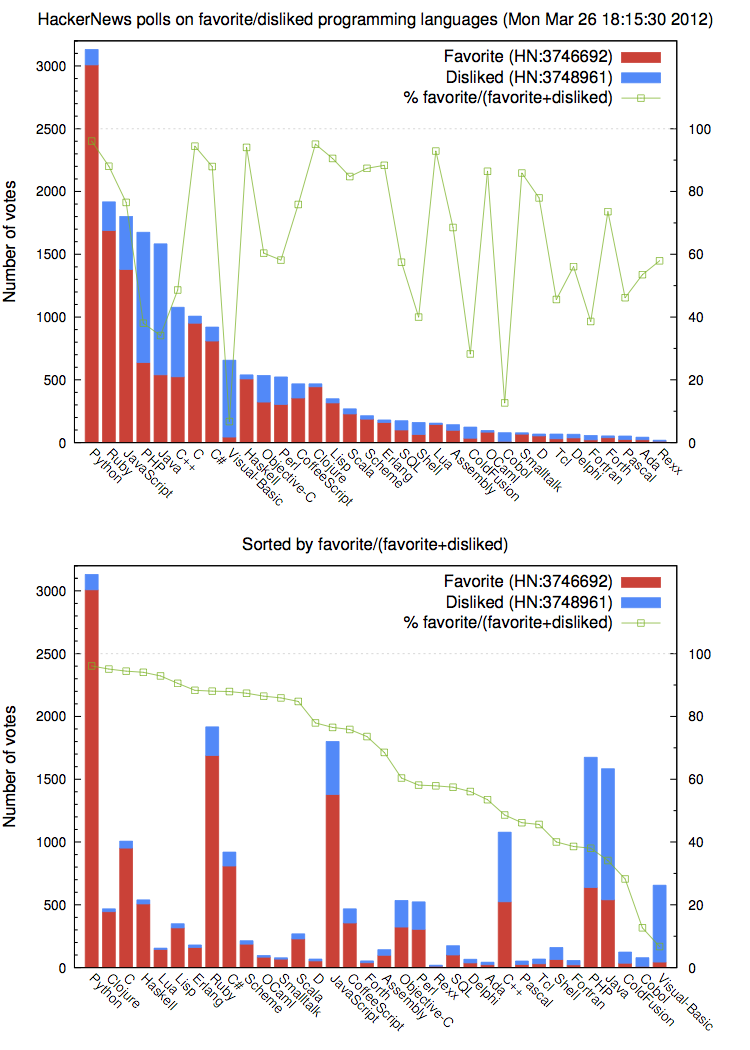
\includegraphics[scale=1]{YourFavoriteDislikeProgramLanguage.png}
	\caption{对编程语言的喜好}
	\label{fig:YourFavoriteDislikeProgramLanguage}
\end{figure}

从应用领域来说,C++适用于高性能计算、嵌入式系统、开发服务器软件、游戏、实时系统等。

\subsection{Architectural Requirements}

\begin{itemize}
\item{Easy to seperate \textrightarrow Autonomy(自治,自治权)}
\item{Easy to understand \textrightarrow Understandability}
\item{Easy to extend \textrightarrow Extensibility}
\item{Easy to change \textrightarrow Changeability}
\item{Easy to replace \textrightarrow Replaceability}
\item{Easy to deploy \textrightarrow Deployability}
\item{Easy to scale \textrightarrow Scalability}
\item{Easy to recover \textrightarrow Resilience(恢复力、弹力、顺应力)}
\item{Easy to connect \textrightarrow Uniform Interface}
\item{Easy to afford \textrightarrow Cost-efficiency(for develop\&operation)}
\end{itemize}

Reliability/Fault torlerance/Reusability/Manageability/Monitorability/
Maintainability/Extensibility/Understandability/Auditability/
Performance/Availability/Scalability/Security

\subsection{不要自我重复(DRY - Don’t Repeat Yourself)}

这也许是在编程开发中最最基本的一个信条,就是要告诉你不要出现重复的代码。
我们很多的编程结构之所以存在,就是为了帮助我们消除重复(例如,循环语句,函数,类,等等)。
一旦程序里开始有重复现象的出现(例如很长的表达式、一大堆的语句,但都是为了表达相同的概念),
你就需要对代码进行一次新的提炼,抽象。
一次且仅一次(once and only once,简称OAOO)又称为 Don't repeat yourself(不要重复你自己,简称DRY)或一个规则,
实现一次(one rule, one place)是面向对象编程中的基本原则,程序员的行事准则。旨在软件开发中,减少重复的信息。
DRY的原则是:系统中的每一部分,都必须有一个单一的、明确的、权威的代表:指的是(由人编写而非机器生成的)代码和测试所构成的系统,
必须能够表达所应表达的内容,但是不能含有任何重复代码。当DRY原则被成功应用时,
一个系统中任何单个元素的修改都不需要与其逻辑无关的其他元素发生改变。此外,与之逻辑上相关的其他元素的变化均为可预见的、均匀的,并如此保持同步。
软件重复出现至少会导致以下问题: 

\begin{itemize}
	\item{其中的一个版本会过期}
	\item{代码的责任会四处散开,导致代码难以理解}
	\item{当你修改代码时,需要重复修改很多地方,一不小心就会遗漏}
	\item{你不能很好地进行性能优化}
\end{itemize}

\subsection{单一职责原则(Single Responsibility Principle,SRP)}

单一职责原则\footnote{http://en.wikipedia.org/wiki/Single\_responsibility\_principle}是指一个代码组件
(例如类或函数)应该只执行单一的预设的任务。

\subsection{开放/封闭原则(Open Closed Principle)}

程序里的实体项(类,模块,函数等)应该对扩展行为开放,对修改行为关闭(Open for extension, closed for modification)。
换句话说,不要写允许别人修改的类,应该写能让人们扩展的类。

\subsection{保持简单(Keep It Simple)}

保持简单\footnote{http://en.wikipedia.org/wiki/KISS\_principle}简单化(避免复杂)永远都应该是你的头等目标。
简单的程序让你写起来容易,产生的bug更少,更容易维护修改。

\subsection{用最简单的方法让程序跑起来}

在开发时有个非常好的问题你需要问问自己,“怎样才能最简单的让程序跑起来?”这能帮助我们在设计时让程序保持简单。

\subsection{避免过早优化}

只有当你的程序没有其它问题,只是比你预期的要慢时,你才能去考虑优化工作。
只有当其它工作都做完后,你才能考虑优化问题,而且你只应该依据经验做法来优化。
\begin{quote}
 \emph{Premature optimization is the root of all evil!}
\end{quote}
“对于小幅度的性能改进都不该考虑,要优化就应该是97\%的性能提升:过早优化是一切罪恶的根源” — Donald Knuth。
编程的一个最核心的目的是解决问题,满足用户的需求。先保证解决方案的正确性(确实正确地解决了问题),
再考虑其他一些特性,比如易操作性、运行速度、界面友好等等,经过适当的迭代一般在这些方面就能越来越好。
但是,解决方案的正确性却不一定会慢慢「越来越正确」的,比如用户需要监测一个金融市场指标是否发生了分布性质的突变,
从而根据突变的情况做出不同的决策,结果一个研究小组开发出一套做监测的系统过早地做了优化,
计算速度飞快、用户体验也很好,但是由于研究不到位,使用的基础统计检验整个就是错误的,
由此经过大量性能优化的算法基本也都是白费了。

因此,为了减少无用功,提高一定时间内的有效生产力,先保证解决方案在原理上是正确的,
可以解决问题,可以满足需求,再考虑更高层次的要求,例如性能等等。


\subsection{依赖倒置原则(Dependence Inversion Principle)}

A.高层次的模块不应该依赖于低层次的模块,他们都应该依赖于抽象。

B.抽象不应该依赖于具体,具体应该依赖于抽象。

\subsection{接口隔离原则(Interface Segregation Principle)}

使用多个专门的接口比使用单一的总接口要好。

一个类对另外一个类的依赖性应当是建立在最小的接口上的。

一个接口代表一个角色,不应当将不同的角色都交给一个接口。
没有关系的接口合并在一起,形成一个臃肿的大接口,这是对角色和接口的污染。
“不应该强迫客户依赖于它们不用的方法。接口属于客户,不属于它所在的类层次结构。
”这个说得很明白了,再通俗点说,不要强迫客户使用它们不用的方法,
如果强迫用户使用它们不使用的方法,那么这些客户就会面临由于这些不使用的方法的改变所带来的改变。

\begin{quotation}
The interface-segregation principle (ISP) states that no client should be forced to 
depend on methods it does not use. 
ISP splits interfaces which are very large into smaller and more specific ones 
so that clients will only have to know about the methods that are of interest to them. 
Such shrunken interfaces are also called role interfaces. 
ISP is intended to keep a system decoupled and thus easier to refactor, 
change, and redeploy. ISP is one of the five SOLID principles of Object-Oriented Design,
 similar to the High Cohesion Principle of GRASP.
\end{quotation}

好的接口定义应该是具有专一功能性的,而不是多功能的,否则造成接口污染。
如果一个类只是实现了这个接口的中一个功能,而不得不去实现接口中的其他方法,就叫接口污染。

\subsection{关注点分离(Separation of Concerns)}

好的架构设计必须把变化点错落有致地封装到软件系统的不同部分,为此,必须进行关注点分离。
Ivar Jacobson在《AOSD中文版》中写道:

好的架构必须使每个关注点相互分离,也就是说系统中的一部分发生了改变,
不会影响其他部分。即使需要改变,也能够清晰地识别出哪些部分需要改变。
如果需要扩展架构,影响将会最小化。已经可以工作的每个部分都将继续工作。\subsection{封装变化点}

%\item{提炼原则}

\subsection{不要开发你目前用不到的功能(You Ain’t Gonna Need It,YAGNI原则)}

YAGNI原则指的是只需要将应用程序必需的功能包含进来,
而不要试图添加任何其他你认为可能需要的功能。

%\item{不要让我动脑子}
%\item{为维护者写程序}
%\item{最少意外原则}
%\item{最小化耦合关系}
%\item{最大化内聚性}
%\item{隐藏实现细节}
%\item{笛米特法则(Law of Demeter)}
%\item{代码复用(Code Reuse)}
%\item{职责分离(Separation of Concerns)}
%\item{拥抱变化}

\subsection{合成/聚合复用原则(Composite/Aggregate Reuse Principle,CARP)}

尽量使用合成/聚合,尽量不要使用继承。

\subsection{依赖倒置(Dependency Inversion Principle)}

DIP的两大原则:

1、高层模块不应该依赖于低层模块,二者都应该依赖于抽象。

2、抽象不应该依赖于细节,细节应该依赖于抽象。

具体来讲,依赖倒置的核心思想是针对接口而不是实现编程。
应用DIP可以降低模块之间的耦合度,只要接口保持稳定,
模块可以独立演化而互不影响。

\subsection{读写分离}

OneProxy是平民软件完全自主开发的分布式数据访问层,帮助用户在MySQL/PostgreSQL集群上快速搭建支持分库分表的分布式数据库中间件,
也是一款具有SQL白名单(防SQL注入)及IP白名单功能的SQL防火墙软件。
采用与MySQL Proxy一致的反向协议输出模式,对应用非常简单和透明易用,
让用户畏惧的分库分表(Horizontal Partitioning)工作变得极其简单可控!
基于Libevent机制实现,单个实例可以实现25万的SQL转发能力,用一个OneProxy节点可以带动整个MySQL集群。

互联网企业在开源软件的基础之上打造了足以支撑每天十亿笔交易、支付处理能力的在线系统,
其中分布式架构在其中发挥了关键的作用。在架构里面又分为应用层架构和数据层架构,
应用层架构着重于解决应用之间的远程调用、服务的发现、消息的流转,
数据层架构着重于解决底层数据库、缓存等的透明扩展。关系数据库的水平扩展,
或者说MySQL数据库的水平扩展能力是架构中的关键所在,OneProxy是一款构建在MySQL数据库之上的透明数据访问中间件,
由在互联网行业(电商、互联网金融)工作多年的资深架构师精心打造,旨在降底对上层应用开发要求,
实现对应用基本透明的底层数据库单点切换(Failover)、读写分离、水平拆分功能,
使任何公司都可以轻松地拥有与大型互联网企业一样底层数据库扩展能力,也不用受制于开发语言的限制,以帮助业务实现再一次腾飞。

\subsection{动静分离}

\subsection{数据库表拆分\&分片}

\subsection{主从同步}

\subsection{负载均衡}

\subsection{去中心化}

\subsection{主从分离}

\subsection{服务隔离}

\subsection{灰度部署}

避免上线导致大规模应用故障。

\subsection{异步化}

减少系统之间的强依赖,避免一个服务无法使用整个系统都无法使用的问题。

\subsection{统一监控\&统一日志}

\subsection{技术选型}

淘宝的黄裳讲解淘宝网站架构发展的时候,说起2004年底淘宝为何从PHP 向 Java 转移的事情。
为何转换,他阐述了几个理由,其中一个是非常有趣的:当时的 PHP 缺少一个 IDE。
而合适的 IDE 能够有效提升规模化软件开发的效率。

我们知道eBay在2002年的时候也在Sun技术团队的帮助下,将整个应用架构从C++迁移到J2EE。
也就是 eBay 内部所说的 V3 版本。

选 Windows和选Linux有没有哪个更好,我想说的是,都还不错,
不要以为选Windows就不好(StackOverflow就是.NET平台)。

很多金融机构都是用Windows的平台(你可能会和我争吵国内的银行都不是Windows的平台,
都是Unix的平台,是的,我也是在银行里做过的,中国的银行几乎都是IBM/SUN/ORACLE的领地,
所以,那里都是AIX、RISC600,Solaris,Java,C/C++的地方),
但是国外很多金融机构却更多用的是Windows。

以前淘宝架构师黄裳说过,或许是 PHP 缺少一个IDE ;) 当然实际上不是这样的,
当时的 PHP 远没有现在成熟。比如,PHP 缺少中间件(或许现在也是),
而 Java 当时起码有 Weblogic /Jboss 可用。至于解决方案,Java 相对更为成熟,
从人的角度来说,Java 企业级应用背景的人才更多一些,再说可以得到Sun中国技术团队的协助。
应该是2004年底的技术决定吧,同时间段迁移的还有从 MySQL 迁移到 Oracle ,从 PC 服务器迁移到小型机。这是一个正确的决定。

其实当时最早更换的不是PHP语言,而是MySQL,MySQL当年太弱了,读写性能问题严重,
容易死锁。而阿里当时在Oracle方面的积累非常强大,有冯春培、汪海、Fenng这样的人物(fenng比他们稍微晚点来,来的时候已经换了),
于是数据库就迁移到了Oracle。PHP不具备连接池的功能,一开始弄了一个sqlRelay中间件来充当连接池,
结果这个东东也经常死掉,于是开发语言也必须跟着换,至于为什么换java,fenng已经说的很清楚了。 
当然现在的MySQL已经不是当年的吴下阿蒙了,现在用LAMP架构的话应该能支持很高的流量。

轮回罢了。 当业务快速发展的时候必须靠DB的能力顶上,所以第一批做DB的人冒出了头。 
接下来DB扛不住了,架构上场…… 出了一批架构师。 架构搞好之后,DB就不再那么重要了,
于是开始可以降低Oracle规模了,Mysql上场以及KV出场。 oracle 收购了mysql 要围剿的话,
谁知道几年后是不是 postgresql 上场?

现在国外用PHP很多的,典型的是Facebook。 Java运行时对内存的管理和监控非常方便,之前twitter使用ruby写了一个消息队列,
因为无法管控内存,换成用Scala重写了一个新的消息队列

58同城使用的是 Windows、iis、SQL-Sever、C\# 这条路。
现在很多创业公司可能就不会这么做。58 同城为什么当时选择了这条路?
原因是公司招聘的第一个工程师和第二个工程师只会这个,所以只能走这条路。

网站在不同的阶段遇到的问题不一样,而解决这些问题使用的技术也不一样,
流量小的时候,我们主要目的是提高开发效率,在早期要引入 ORM,
DAO 这些技术。随着流量变大,使用动静分离、读写分离、主从同步、垂直拆分、CDN、MVC等方式不断提升网站的稳定性。
面对更大的流量时,通过垂直拆分、服务化、反向代理、开发框架(站点/服务)等等,不断提升高可用。
在面对上亿级的更大流量时,通过中心化、柔性服务、消息总线、自动化(回归,测试,运维,监控)来迎接新的挑战。
未来的就是继续实现 移动化,大数据实时计算,平台化

\subsection{一般网站架构}

网站架构一般分为网页缓存层、负载均衡层、Web层、数据库层、文件服务器层。
Nginx已经具备Squid所拥有的Web缓存加速功能。此外,Nginx对多核CPU的利用胜过Squid,
现在越来越多的架构师都喜欢将Nginx同时作为”负载均衡服务器”与”Web缓存服务器”来使用




\section{编码规范(Programming Specification)/编程风格(Programming Style)}

编程规范就是为了便于自己和他人阅读理解源程序,而制定的一个规范。
编程规范只是一个规范,也可以不遵守,但是要做一个有良好编程风格的程序员,
就一定要遵守编程规范,不仅方便自己以后的阅读,也方便与其他程序员的交流。
代码一旦编写完毕,剩下的就是阅读和修改。所以,需要谨慎对待代码的撰写。
编码约定的细节要达到这样的精确度:在编写完软件之后,
几乎不可能改变(翻新)软件所遵循的编码约定。
用规范和约定来使大脑从记忆不同代码段的随意性、
偶然性差异中解脱出来\footnote{《代码大全》34.1节}。
不管有多少人共同参与同一项目,一定要确保每一行代码都像是同一个人编写的。

\subsection{良好编码习惯}

\begin{enumerate}
\setcounter{enumi}{0}
\item{确保没有任何警告(warnings)}
\item{去掉所有没有用到的usings,编码过程中尽量去掉多余代码}
\item{尽早且经常的重构代码(Refactor often and sooner)}
\item{请确保你了解SOLID\footnote{http://en.wikipedia.org/wiki/SOLID\_\%28object-oriented\_design\%29}原则}

在程序设计领域,SOLID (\textbf{单一功能、开闭原则、里氏替换、接口隔离}以及\textbf{依赖反转})是由罗伯特·C·马丁在21世纪早期引入的记忆术首字母缩略字,指代了面向对象编程和面向对象设计的五个基本原则。当这些原则被一起应用时,它们使得一个程序员开发一个容易进行软件维护和扩展的系统变得更加可能。SOLID所包含的原则是通过引发编程者进行软件源代码的代码重构进行软件的代码异味清扫,从而使得软件清晰可读以及可扩展时可以应用的指南。SOLID被典型的应用在测试驱动开发上,并且是敏捷开发以及自适应软件开发的基本原则的重要组成部分
\item{始终遵循命名规范\footnote{更多命名规范见《代码大全》第11章~~变量名的力量}。
一般而言变量参数使用驼峰命名法(dataOper),方法名和类名使用Pascal命名法(DataOper),
本标准中摒弃使用匈牙利命名法(data\_Oper)}
\item{如果需要多次串联,请使用Stringbuilder代替string,这可以节省堆内存}
\item{为了避免在阅读代码时不得不滚动源代码编辑器,每行代码或注释在1024*800的分辨率下不得超过一显示屏,
代码中方法的行数不超过30到40行}
\item{避免for/foreach循环嵌套和if条件嵌套(Restrict all code to very simple control flow constructs)}
\item{在一个尽可能小的范围内赋值或初始化变量、结构等,
限制全局变量的使用(Data objects must be declared at the smallest possible level of scope)。
降低变量的作用域有如下好处:
其一:变量被无意修改的可能性降低;
其二:使代码更具有可读性;
其三:当需要对大程序分拆成小的子程序时,
降低变量的作用域(Comments on Minimizing Scope)会使分拆起来更加简单\footnote{《代码大全》10.4节}。
全局变量也会大大增加需要兼顾的代码的比例\footnote{《代码大全》34.1节}。}
\item{重视日志的采集,保证所有的系统异常和关键信息有记录}	
\item{使用标准库函数和公共函数}	
\item{足够的单元测试加上持续集成工具让你修改代码时更加有自信}
\item{修改越是细微越好,如果大量的修改后引入了错误,会很难发现到底是哪一步修改所导致}
\item{所有类型、方法、参数、变量的命名不推荐缩写,
包括大家熟知的缩写,例如 msg,使用缩写常见的2个问题:
一是代码的读者可能不理解这些缩写,
其他程序员可能会用多个缩写代表相同的词,从而产生不必要的混乱.
如果没有项目级的标准缩写文档,不推荐使用缩写.}
\item{方法应避免过多参数,合理的参数个数,其上限大概是7个左右\footnote{《代码大全》7.1节.}}
\item{为变量指定单一用途,避免在2个位置把同一变量用于不同用途,
例如temp变量在程序里2处用到,但代表不同的含义\footnote{《代码大全》10.8节}}
\item{记住典型的布尔变量命名:done,error,found,success或ok}
\item{将复杂度降到最低是高质量代码的关键}
\item{可考虑将大的工具类拆分成互不干扰的小的工具类,
如NetworkUtil可拆分成HttpUtil,FTPUtil,TelnetUtil}
\end{enumerate}	

\subsection{变量(Variable)命名规范}


\begin{itemize}
	\item{使用可搜索的名字} 避免使用Magic Number,避免使用单字母,或出现频率极高的短字母组合。
	\item{名字尽量来自解决方案领域或问题领域} 术语、算法名、模式名、数学术语尽管用。如AccountVisitor:Visitor模式实现的Account类。
\end{itemize}

1)  使用名词、名词性词组或者名词地缩写来命名。

2)  使用Camel Case,与.NET的风格保持一致(consistent with the Microsoft's .NET Framework and easy to read)。

3)  变量名中不使用下划线 (\_)。

4)  成员变量不要使用匈牙利命名法。

5)  只要合适,在变量名的末尾追加计算限定符(Avg、Sum、Min、Max、Index)。

6)  在变量名中使用互补对,如 min/max、begin/end 和 open/close。

7)  布尔变量包含Is,这意味着 Yes/No 或 True/False 值,如 fileIsFound。

8)  状态变量命名时,避免使用诸如 Flag 的术语。
状态变量不同于布尔变量的地方是它可以具有两个以上的可能值。
不是使用 documentFlag,而是使用更具描述性的名称,如 documentFormatType。

10) 数组后加Array,列表后加List,字典后加Dictionary,DataSet后加Set。

\subsection{命名空间(Namespace)命名规范}

1)  使用 公司名.产品名 这样的格式。

2)  Namespace中类的依赖关系应该体现在命名上,比如System.Web.UI.Design中的类以来于System.Web.UI。

3)  使用 Pascal大小写形式命名。

4)  当商标(产品名)的命名风格和Pascal风格不符时,以商标(产品名)为准。

5)  在语意合适的情况下使用复数,比如System.Collections。例外是缩写和商标的情况。

6)  Namespace的名字不一定和Assembly一一对应。

\subsection{类(Class)命名规范}

1)  使用名词或者名词性词组命名class。

2)  使用 Pascal case,与.NET的命名保持一致(consistent with the Microsoft's .NET Framework and easy to read)。

3)  文件名应和类名相同。

4)  保守地使用缩写。

5)  不使用type前缀,例如C来标识Class。比如,使用FileStream而不是CFileStream。

6)  不使用下划线。

7)  偶尔的在Class名称组成中需要使用I开头的时候,比如IdentityStore,just use it。

8)  在合适的时候,使用单词复合来标识从某个基类继承而来。比如xxxException。

\subsection{类(Class)注释规范}\label{ClassNamingSpecification}

\begin{lstlisting}[language={[Sharp]C}]
/*------------------------------------------------
<copyright file="$safeitemrootname$.cs" company="RRMall">
Copyright (c) RRMall.All Rights Reserved.
</copyright>
CLRVersion:$clrversion$
NameSpace:$rootnamespace$ 
Author:$username$
Email:jiangxiaoqiang@renrenmall.com
CreateDate:$time$
Stamp:$guid10$
UserDomain:$userdomain$

---------------------------
Modifier:
ModifyDate:
ModifyDescription:
-----------------------------------------------*/
namespace $rootnamespace$
{
	using System;
	
	/// <summary>
    /// Write the class summary. 
    /// </summary>
    public class $safeitemrootname$
    {
    }
}		
\end{lstlisting}

\subsection{接口(Interface)命名规范}

1)  使用名词或者名词性词组命名Interface。

2)  使用 Pascal case。

3)  保守地使用缩写。

4)  在interface 名称前加上字母I来表示type是interface。

5)  在某个class是某个interface地标准实现地时候,用类似的名字来命名它们,仅仅在interface的名称前面多个I。

6)  不要使用下划线。

7)  文件名应和类名相同。

\subsection{常量命名规范}

常量名也应当有一定的意义,格式为 NOUN 或 NOUN\_VERB。常量名均为大写,字之间用下划线分隔。

例:

     private const bool   WEB\_ENABLEPAGECACHE\_DEFAULT           = true;

     private const int    WEB\_PAGECACHEEXPIRESINSECONDS\_DEFAULT = 3600;

     private const bool   WEB\_ENABLESSL\_DEFAULT                 = false;

注:

变量名和常量名最多可以包含 255 个字符,但是,超过 25 到 30 个字符的名称比较笨拙。此外,要想取一个有实际意义的名称,清楚地表达变量或常量的用途,25 或 30 个字符应当足够了。

\subsection{方法(Method)命名规范}

1)  使用动词或者动词性词组命名。

2)  使用Pascal case。

3) 如果方法返回的类型为bool类型,则其前缀为Is、Can 或者Try。

\subsection{事件(Event)命名规范}

1)  使用Pascal case。

2)  不要使用匈牙利命名法。

3)  在event handler名字中使用EventHandler后缀。

4)  指定两个名字分别为sender和e的参数。sender参数代表了发出事件的对象。sender参数总是类型object,即使可能使用一个更加精确的类型。和事件相关的状态封装在名字为e的event class的实体之中。给e指定恰当而且明确的event class。

5)  使用EventArgs后缀命名事件参数class。

6)  考虑使用动词命名事件。使用进行时态来标识事件正在进行之中,使用完成时态标识事件已经完成,不要使用BeforeXxx/AfterXxx命名法。

7)  不要在事件声明中使用前缀和后缀,比如,用Close而不是OnClose。

8)  一般应同时提供一个名字为OnXxx的protected method供派生类来改写。

9) 事件以其对应的委托类型,去掉EventHandler后缀,并加上On前缀构成。

\subsection{数据库命名规范}

1)总是使用单数名称,不管是表名称还是列名称\footnote{《C\#高级编程(第7版)第30.9.3节》}。例如Product而不是Products。	

2)存储过程名称不要以sp\_开头,因为SQL Server系统存储过程都是以sp\_开头,所以sp\_Widget会给人是否为标准存储过程的疑惑。

\subsection{创建类标准模板}

在新建类时,Visual Studio会自动调取类模板,通过修改类模板,在新建类时自动添加类注释,
避免手工注释的麻烦。模板的路径为:
\begin{lstlisting}
D:\Program Files (x86)\Microsoft Visual Studio 12.0\Common7\IDE\ItemTemplates\CSharp\Code\2052\Class
\end{lstlisting}

将类的注释规范(在节\ref{ClassNamingSpecification}中)粘贴到模板里面即可,如果想定义其他如新建接口的模板,新建web类模板,
在临近的文件夹将之替换即可,添加类
的注释规范之后可立即生效,不必重新启动Visual Studio 2013。一个标准的用于新建模板类的模板
如下代码片段所示(新建的类通过StyleCop检查):

\begin{lstlisting}[language={[Sharp]C}]
/*------------------------------------------------
<copyright file="$safeitemrootname$.cs" company="RRMall">
Copyright (c) RRMall.All Rights Reserved.
</copyright>
CLRVersion:$clrversion$
NameSpace:$rootnamespace$ 
Author:$username$
Email:jiangxiaoqiang@renrenmall.com
CreateDate:$time$
Stamp:$guid10$
UserDomain:$userdomain$

---------------------------
Modifier:
ModifyDate:
ModifyDescription:
-----------------------------------------------*/
namespace $rootnamespace$
{
	using System;
	
	/// <summary>
    /// Write the class summary. 
    /// </summary>
    public class $safeitemrootname$
    {
    }
}
\end{lstlisting}

\subsection{文件夹命名}

在C\#开发中经常遇到添加新文件夹的情况,以下列出了一些常见的命名
以供参考。

\begin{tabular}{ll|ll}
	\multirow{1}{*}{}			
	& \multicolumn{1}{c}{}
	& \multicolumn{1}{c}{}
	& \multicolumn{1}{c}{}\\
	Client & 客户端部署文件夹 & Wrapper & 包裹\\
	Service & 服务端部署文件夹 & Factory & 工厂\\	
	Control & 控件存放文件夹 & FactoryMethod & 工厂方法\\
	Controller & 控制器 & Facade & 外观\\
	ReportCenter & 报表中心 & Builder & 建造者\\
	View & 界面 & Common & 公共\\
	ViewModel & 界面模型 & Security & 安全\\
	Filter & 过滤器 & Config & 配置\\
	Config & 配置文件 & Adapter & 适配器\\
	Business & 业务逻辑 & Component & 组件 \\
	Core & 核心 & Widget & 物件\\
	Utility & 工具 & Menu & 菜单\\
	Entity & 实体 & Static & 静态\\
	Pattern(s) & 模式 & Template & 模板\\
	Handler & 处理者 & Public\footnotemark[1] & 公共\\
	Action & 动作 & Route & 路由\\
	Base & 基 & Proxy & 代理\\ 
	Library & 库 & Tools & 工具库 \\
    Platform & 平台 & NetworkProcess & 网络进程 \\
    Storage & 存储的共享代码 & Loader & 资源加载器\\
    Preview\footnotemark[2] & 预演 & SubView & 子视图\\
    Network & 网络 & Category & 分类\\
    Vendor\footnotemark[3] & 第三方 & Expand & 扩展\\
\end{tabular}

\footnotetext[1]{Base用于存放一些抽离提取或以共用的可被继承的内容}
\footnotetext[2]{Preview用于存放一些练习的功能页面,集成一些第三插件实例或者实例代码都可以放在里面}
\footnotetext[3]{Vender(第三方)存放一些可能被修改的第三方插件及一些自个封装插件}

\subsection{目录结构}

\begin{lstlisting}
root
	|--Source
	|	|--Plugin
	|	|	|--Plugin 1
	|	|	|--Plugin 2
	|	|--Project A
	|	|--Project B
	|--Test
	|	|--Test Project A
	|	|--Test Project B
	|--Tool
	|	|--Tool1
	|	|--Tool2	
\end{lstlisting}


\subsection{代码规范检查}

StyleCop analyzes C\# source code to enforce a set of style and consistency rules. It can be run from inside of Visual Studio or integrated into an MSBuild project. StyleCop has also been integrated into many third-party development tools.

不是拿到需求就开始写代码,而是先考虑清楚。 
需求是否合理,是否能解决用户的问题,逻辑上是否有模糊或不完备的地方。 
然后考虑设计的问题,流程图是什么样的,类图是什么样的,接口是什么样的,
对架构和模块的影响是什么样的,考虑清楚后才开始写代码。

\subsection{避免空引用异常(Null Reference Exception)}

在使用对象之前做非空检查,
保持代码的健壮性,获取的Request对象进行非空检查。

\begin{lstlisting}[language={[Sharp]C}]
\\推荐:对象为空时赋给进行默认值
var sellerId = (sellerModelList == null) ? 0 : sellerModelList[0].sellerId;

\\不推荐写法
string requestUrl = Request.Url.OriginalString;
\\推荐写法
var requestUrlObj = Request.Url;
if (requestUrlObj != null)
{
    string requestUrl = requestUrlObj.OriginalString;
}
\end{lstlisting}

\section{运行效率(Performance)}

\subsection{避免开辟内存}

\subsection{避免装箱}

\subsection{常见数据结构及复杂度}

搜索一个好的Hash表会得到O(1)复杂度,
糟糕的排序算法具有O(n\^2)复杂度,
最好的排序算法具有O(n*log(n))复杂度,
搜索一个阵列会得到O(n)复杂度,
搜索一个均衡的树会得到O(log(n))复杂度。 

\begin{tabular}{l|l|l|l|l}
	\multirow{1}{*}{}			
	& \multicolumn{1}{c}{}
	& \multicolumn{1}{c}{}
	& \multicolumn{1}{c}{}
	& \multicolumn{1}{c}{}\\
	Data Structure & Add & Find & Delete & GetByIndex\\
	\hline
	Array (T[]) & O(n) & O(n) & O(n) & O(1)\\
	\hline
	Linked list (LinkedList<T>) & O(1) & O(n) & O(n) & O(n)\\
\end{tabular}

\paragraph{哈希表和阵列}

\begin{itemize}
	\item{一个哈希表可以只装载一半到内存,剩下的哈希桶可以留在硬盘上}
	\item{用阵列的话,你需要一个连续的内存空间。如果加载一个大表,很难分配连续的内存空间}
	\item{用哈希表,可以选择需要的关键字}
\end{itemize}

\section{数据库}

\subsection{字段}

\paragraph{表中应该避免可为空的列}虽然表中允许空列,但是,
空字段是一种比较特殊的数据类型。数据库在处理的时候,
需要进行特殊的处理。如此的话,就会增加数据库处理记录的复杂性。
当表中有比较多的空字段时,在同等条件下,数据库处理的性能会降低许多。

要求二:表不应该有重复的值或者列。

要求三:表中记录应该有一个唯一的标识符。

要求四:数据库对象要有统一的前缀名。

要求五:尽量只存储单一实体类型的数据。

\paragraph{表的主键(ID、PKID)应当不具有任何业务含义}

表通过主键来保证每条记录的唯一性,表的主键应当不具有任何业务含义,
因为任何有业务含义的列都有改变的可能性。
关系数据库学的最重要的一个理论就是:不要给关键字赋予任何业务意义。
假如关键字具有了业务意义,当用户决定改变业务含义,
也许他们想要为关键字增加几位数字或把数字改为字母,
那么就必须修改相关的关键字。一个表中的主关键字有可能被其他表作为外键。
就算是一个简单的改变,譬如在客户号码上增加一位数字,
也可能会造成极大的维护上的开销。为了使表的主键不具有任何业务含义,
一种解决方法是使用代理主键,
例如为表定义一个不具有任何业务含义的ID字段(也可以叫其他的名字),
专门作为表的主键\footnote{孙卫琴《精通Hibernate:Java对象持久化技术详解》}。
考虑每个表增加必备字段,用于记录该笔数据的创建时间,创建人,最后修改人,最后修改时间等等信息。

\begin{lstlisting}[language=SQL]
[ID] [int] NOT NULL,
[Status] [int] NULL,
[CreatedDate] [datetime] NULL,
[CreatedBy] [nvarchar] (10) COLLATE SQL_Latin1_General_CP1_CI_AS NULL,
[RevisedDate] [datetime] NULL,
[RevisedBy] [nvarchar] (10) COLLATE SQL_Latin1_General_CP1_CI_AS NULL,
[IsDel] [tinyint] NULL,
[Remark] [nvarchar] (2048) NULL,
[RowGuid] [nvarchar] (38) NULL,
[Sort] [int] NULL
\end{lstlisting}

GUID是一个128位长的数字,一般用16进制表示。
算法的核心思想是结合机器的网卡、当地时间、一个随即数来生成GUID。
从理论上讲,如果一台机器每秒产生10000000个GUID,则可以保证(概率意义上)3240年不重复。

\subsection{登录用户权限}


\section{环境}

\subsection{开发环境}

现在所使用的编程语言无非就两种,
一种是解释型(Interpreted Language)的语言,
另一种就是编译后才能够执行的语言。

\begin{quotation}
An interpreted language is a programming language for 
which most of its implementations execute instructions directly, 
without previously compiling a program into machine-language instructions. 
The interpreter executes the program directly, 
translating each statement into a sequence of one or more subroutines already compiled into machine code.
\end{quotation}

解释型语言最大的弱点就是能够被反编译\footnote{《加密与解密》(第3版)第四篇篇头语}。
解释性语言先是编译为中间语言,然后才编译为计算机可以识别的机器语言。
解释型语言每执行一次就需要编译一次,解释性语言开发的程序需要依赖于特定的编译框架。
但是解释性语言有跨平台的优点。

\begin{quotation}
A compiled language is a programming language whose implementations 
are typically compilers (translators that generate machine code from source code), 
and not interpreters (step-by-step executors of source code, where no pre-runtime translation takes place).
\end{quotation}

编译型语言(Compiled Language)的程序执行效率相对较高,而且只需要编译一次,
运行时不需要编译。后者由于程序执行速度快,同等条件下对系统要求较低,
因此像开发操作系统、大型应用程序、数据库系统等时都采用它,
像C/C++、Pascal/Object Pascal(Delphi)等都是编译语言,
而一些网页脚本、服务器脚本及辅助开发接口这样的对速度要求不高、
对不同系统平台间的兼容性有一定要求的程序则通常使用解释性语言,
如JavaScript、VBScript、Perl、Python、Ruby、MATLAB 等等。
项目开发语言选择解释型的语言C\#,
项目开发所用的工具以及环境如下表所示。

\begin{tabular}{c|l|l}
	\multirow{1}{*}{项}			
	& \multicolumn{1}{c}{名称}
	& \multicolumn{1}{|c}{版本}\\
	\hline
	开发工具 & Visual Studio & 2013\\
	日志组件 & log4net & 1.2.13.0\\	
	单元测试组件 & NUnit & 2.6.4\\
	代码规范检查工具 & StyleCorp & 4.7\\	
	数据库 & SQL Server & 2008 R2\\
	源码管理工具 & Visual SVN & 2.7.11\\
	Json处理与转换 & Json.NET & 4.5.11.15520\\
	运行时环境 & .NET Framework & 4.0\\
	BS界面 & easyUI & 1.2.2\\
	持续集成 & CruiseControl.NET & 1.8.5.0\\
	接口通信 & WCF(RESTful) & .NET 4.0\\
	WCF REST调试工具 & HttpRequester & 2.1.1 \\
	WCF REST调试工具 & RestClient & 2.0.3 \\
	Json浏览插件 & JsonViewer & \\
	REST调试 & Rest Client for Chrome & \\
	WCF认证 & RSA签名 & \\
	Web调试 & FireDebug & 2.0.12\\
	RESTful接口 & NodeJS & 4.1.1\\
	NodeJS框架 & Express & 4.13.1\\
	数据库管理工具 & HeidiSQL & 9.3.0.4984\\
	接口压力测试 & JMeter & 2.13\\
	WCF测试 & WCF Storm & \\
	Google Cookie管理 & EditThisCookie & 1.4.1 \\
	VS代码缩进提示插件 & Indent Guids & \\
	代码性能分析 & PerfView & 1.8.0.0  \\ 
	HTTP调试 &  Fiddler & 4.6.1.4\\		
    网页性能优化 & MiniProfiler & latest\\
    后端性能优化 & dotTrace & 10.0.0.2(Commercial)\\
    内存泄漏检测 & dotMemory & 10.0.0.2(Commercial)\\
    Rest客户端 & RestSharp & latest\\
    Markdown编辑器 & Haroopad & 0.13.1\\		
    \end{tabular}

\subsubsection{Visual Studio Code}

在Fedora中安装完毕后的路径为:

\begin{lstlisting}
/usr/share/code
\end{lstlisting}

运行文件夹下的code文件即可。

\subsection{Web Server}

\subsubsection{OpenResty(BSD)}

OpenResty(也称为 ngx\_openresty)是一个全功能的Web应用服务器。
它打包了标准的Nginx核心,很多的常用的第三方模块,以及它们的大多数依赖项。
通过众多进行良好设计的Nginx模块,
OpenResty有效地把Nginx服务器转变为一个强大的Web应用服务器,
基于它开发人员可以使用Lua编程语言对Nginx核心以及现有的各种Nginx C模块进行脚本编程,
构建出可以处理一万以上并发请求的极端高性能的Web应用。
OpenResty 致力于将你的服务器端应用完全运行于 Nginx 服务器中,
充分利用 Nginx 的事件模型来进行非阻塞 I/O 通信。
不仅仅是和 HTTP 客户端间的网络通信是非阻塞的,
与MySQL、PostgreSQL、Memcached、以及 Redis 等众多远方后端之间的网络通信也是非阻塞的。
因为 OpenResty 软件包的维护者也是其中打包的许多 Nginx 模块的作者,
所以 OpenResty 可以确保所包含的所有组件可以可靠地协同工作。

基于OpenResty:优酷。

\subsubsection{Tengine}

Tengine是由淘宝网发起的Web服务器项目。
它在Nginx的基础上,针对大访问量网站的需求,
添加了很多高级功能和特性。Tengine的性能和稳定性已经在大型的网站如淘宝网,
天猫商城等得到了很好的检验。它的最终目标是打造一个高效、稳定、安全、易用的Web平台。

基于Tengine:凤凰网、淘宝、土豆。

\subsubsection{Phusion Passenger}

Phusion Passenger是一个流行的Web应用服务器,它最初是针对Ruby的,
现在也支持Node.js应用。在今年的早些时候该功能被引入了Passenger的企业版中,
但是现在已经开源并随着最近的4.0.21免费版发布。
Passenger能与Apache或者Nginx Web服务器集成,
旨在成为一个服务、监控和扩展Web应用程序的完整解决方案。
Phusion公司的 总部位于荷兰 ,他们宣称在Passenger中运行 Node.js 应用的好处包括:
多租户——通过最小的配置运行一些应用的能力
监控——自动启动Node.js进程、如果进程崩溃了则重启它们
扩展——根据要处理的请求的数量增加或者减少进程的数量
统计——帮助显示运行中进程的状态的工具
Passenger的作者 还指出 ,与Apache/Nginx集成还带来了其他的好处,
例如:加速了静态文件服务,阻止了很多常见的攻击和慢客户端。

\subsection{Apache}

配置文件位置(根据不同的操作系统而定):

\begin{lstlisting}
/etc/apache2/httpd.conf
/etc/apache2/apache2.conf
/etc/httpd/httpd.conf
/etc/httpd/conf/httpd.conf
\end{lstlisting}




\subsection{常见架构}

\begin{tabular}{c|l|l|l|l}
	\multirow{1}{*}{架构名称}
	& \multicolumn{1}{c}{OS}
	& \multicolumn{1}{|c}{数据库}			
	& \multicolumn{1}{|c}{服务端}
	& \multicolumn{1}{|c}{客户端}\\
	\hline
	MEAN & Linux/Windows & MongoDB & NodeJS+Express & AngularJS\\
	LAMP & Linux & MySQL & Apache Tomcat & Perl/PHP/Python\\
	WAMP & Windows &  MySQL/MariaDB & Apache Tomcat & Perl/PHP/Python\\
	LNMP & Linux & MySQL & Nginx & PHP\\
	WSIC & Windows & Microsoft SQL Server & IIS & C\#\\    			
\end{tabular}

\subsection{主流平台}

\begin{itemize}
\item{Rails}
\item{Java EE平台}
\item{LAMP平台}
\item{Microsoft .NET平台}
\item{Django}
\end{itemize}

%\subsection{项目结构}

%	\begin{figure}[htbp]
%	\centering
%	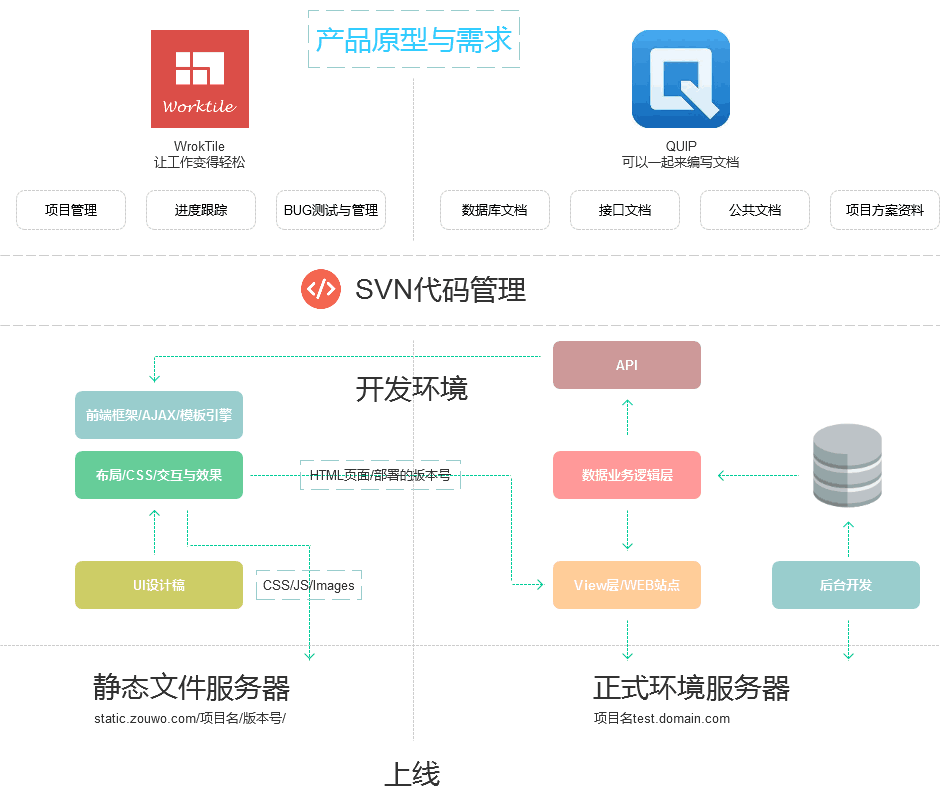
\includegraphics[scale=0.5]{ProjectCollabarate.png}
%	\caption{项目整体结构}
%	\label{ProjectCollabarate}
%	\end{figure}
%	
%	\begin{figure}[htbp]
%	\centering
%	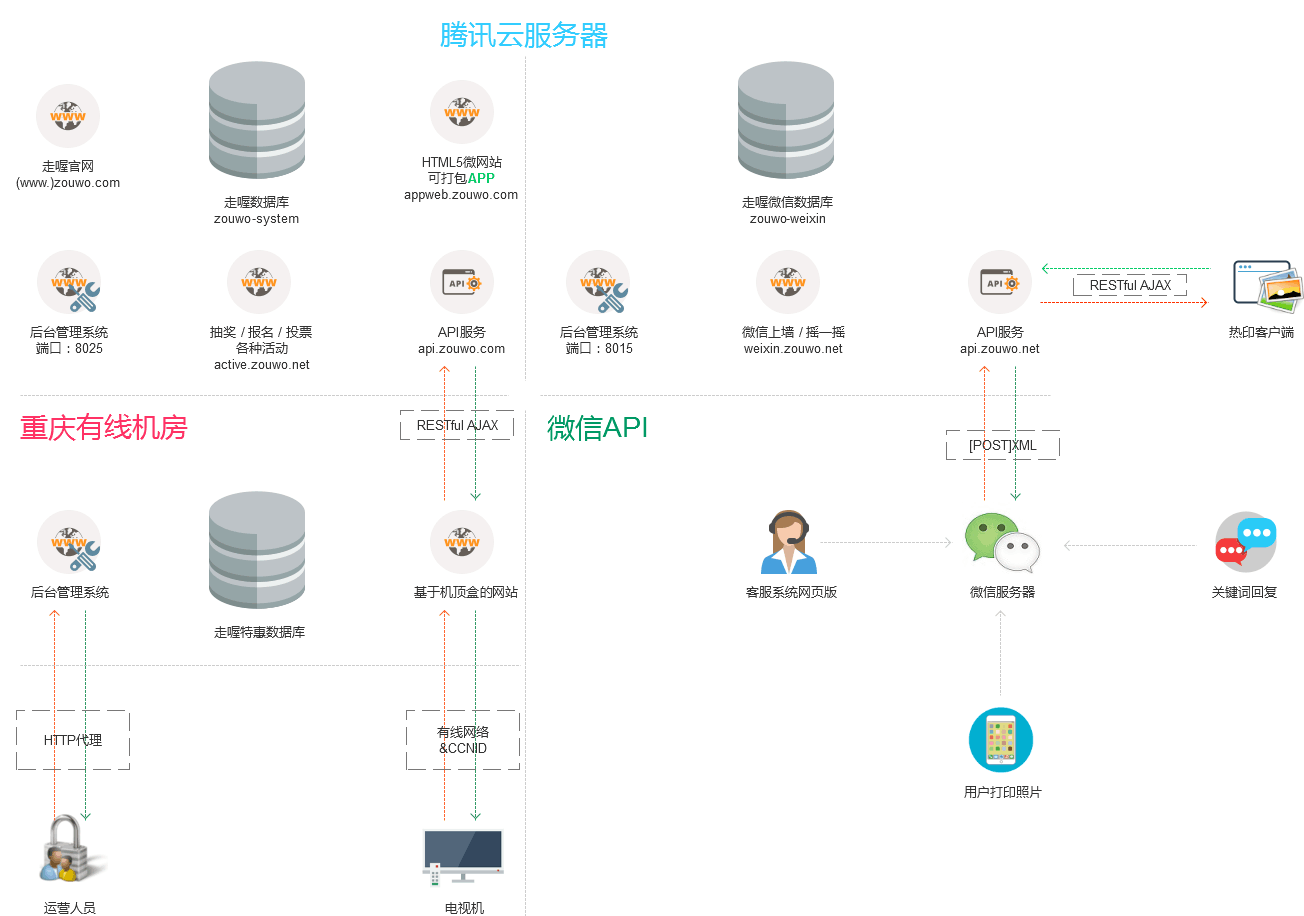
\includegraphics[scale=0.35]{ProductRelation.png}
%	\caption{产品关系}
%	\label{ProductRelation}
%	\end{figure}

\clearpage
\mbox{}         
\clearpage

\chapter{WCF}
\label{sec:wcf}

Windows Communication Foundation(WCF)是由微软发展的一组数据通信的应用程序开发接口,
可以翻译为Windows通讯接口,它是.NET框架的一部分。由 .NET Framework 3.0 开始引入。
WCF的最终目标是通过进程或不同的系统、通过本地网络或是通过Internet收发客户和服务之间的消息。
WCF合并了Web服务、.net Remoting、消息队列和Enterprise Services的功能并集成在Visual Studio中。
WCF专门用于面向服务开发。
WCF与其他面向服务技术之间(ASP.NET \textbackslash J2EE \textbackslash Web Service技术等)最大的区别在于传输可靠性(Transport Reliability)与消息可靠性(Message Reliability)。
传输可靠性(例如通过TCP传输)在网络数据包层提供了点对点保证传递(Point-to-Point Guaranteed Delivery),
以确保数据包的顺序无误。传输可靠性不会受到网络连接的中断或其他通信问题的影响。
.net Remoting是在DCOM等基础上发展起来的一种技术,它的主要目的是实现跨平台、跨语言、穿透企业防火墙,
这也是他的基本特点,与WebService有所不同的是,它支持HTTP以及TCP信道,
而且它不仅能传输XML格式的SOAP包,也可以传输传统意义上的二进制流,这使得它变得效率更高也更加灵活。
而且它不依赖于IIS,用户可以自己开发(Development)并部署(Dispose)自己喜欢的宿主服务器,
所以从这些方面上来讲Web Service其实上是.net Remoting的一种特例。
.net Remoting主要用于C/S结构项目,将.net Remoting采用TCP通讯,比Web Service效率高。

WCF的配置编辑可用微软提供的工具\textbf{SvcConfigEditor.exe},
该工具存放在C:\textbackslash Program Files (x86)\textbackslash Microsoft SDKs\textbackslash Windows\textbackslash v8.1A\textbackslash bin\textbackslash NETFX 4.5.1 Tools下。
查看跟踪日志可用微软提供的工具\textbf{SvcTraceViewer.exe},
在相同的目录下。
两种常见的分布式应用架构风格包括:DO(分布式对象)、RPC(远程过程调用)。
这两种架构风格在企业应用中得到了广泛的应用,
然而,Web架构的设计者们却有意避免采用这两种架构风格。
主要的原因是运行Web应用的互联网环境,与运行企业应用的企业内网环境有很大的差别。 

\section{基础应用}

REST可以降低开发的复杂度,提高系统的可伸缩性,增强系统的可扩展性,简化应用系统之间的集成,
一些新产品的开发甚至已经几乎完全抛弃了传统的类似JSP的技术,转而大量使用REST风格的构架设计, 即在服务器端所有商业逻辑都以REST API的方式暴露给客户端,所有浏览器用户界面使用widget,Ajax,HTML5 等技术,
用 HTTP 的方式与后台直接交互。
WCF主要是设计为RESTful API供客户端(手机、平板、桌面电脑、其他专用设备...)调用,
如下是RESTful API设计建议的原则\footnote{参考阮一峰的博客:www.ruanyifeng.com/blog/2011/09/restful.html},供参考。

\begin{itemize}
\item{API与用户的通信协议,总是使用HTTPS协议}
\item{应该尽量将API部署在专用域名之下,如\url{https://api.example.com}。
如果确定API很简单,不会有进一步扩展,
可以考虑放在主域名下,如\url{https://example.org/api/}}
\item{在RESTful架构中,每个网址代表一种资源(resource),
所以网址中不能有动词,只能有名词,而且所用的名词往往与数据库的表格名对应。
一般来说,数据库中的表都是同种记录的"集合"(collection),
所以API中的名词也应该使用复数}
\item{API的版本号不应加入URI中\footnote{http://www.informit.com/articles/article.aspx?p=1566460},
因为不同的版本,可以理解成同一种资源的不同表现形式,
所以应该采用同一个URI。版本号可以在HTTP请求头信息的Accept字段中进行区分}
\item{针对不同操作,服务器向用户返回的结果应该符合以下规范}
\begin{lstlisting}
GET /collection:返回资源对象的列表(数组)
GET /collection/resource:返回单个资源对象
POST /collection:返回新生成的资源对象
PUT /collection/resource:返回完整的资源对象
PATCH /collection/resource:返回完整的资源对象
DELETE /collection/resource:返回一个空文档
\end{lstlisting}
\item{如果记录数量很多,服务器不可能都将它们返回给用户。API应该提供参数,过滤返回结果}
\begin{lstlisting}
?limit=10:指定返回记录的数量
?offset=10:指定返回记录的开始位置。
?page=2&per_page=100:指定第几页,以及每页的记录数。
?sortby=name&order=asc:指定返回结果按照哪个属性排序,以及排序顺序。
?animal_type_id=1:指定筛选条件
\end{lstlisting}
\item{API的身份认证应该使用OAuth 2.0框架}
\item{服务器返回的数据格式,应该尽量使用JSON,避免使用XML}
\item{服务器向用户返回的状态码\footnote{HTTP状态码:http://www.w3.org/Protocols/rfc2616/rfc2616-sec10.html}
(Status Code)和提示信息,常见的有以下一些(方括号中是该状态码对应的HTTP动词)}

\begin{lstlisting}
200 OK - [GET]:服务器成功返回用户请求的数据,该操作是幂等的(Idempotent)
201 CREATED - [POST/PUT/PATCH]:用户新建或修改数据成功
204 NO CONTENT - [DELETE]:用户删除数据成功
400 INVALID REQUEST - [POST/PUT/PATCH]:用户发出的请求有错误,服务器没有进行新建或修改数据的操作,该操作是幂等的
404 NOT FOUND - [*]:用户发出的请求针对的是不存在的记录,服务器没有进行操作,该操作是幂等的
500 INTERNAL SERVER ERROR - [*]:服务器发生错误,用户将无法判断发出的请求是否成功
\end{lstlisting}
\end{itemize}

接口调用链接的命名原则:/项目名称/模块名/接口名?{参数集合}。
由于每个接口皆返回状态码,错误消息、提示等公共信息,
新建一个基类定义公共信息。

\begin{lstlisting}[language={[Sharp]C}]
public class BaseModel
{
    #region 错误码

    private int _errorCode;

    public int ErrorCode
    {
        get { return _errorCode; }
        set { _errorCode = value; }
    }

    #endregion

    #region 错误消息

    private string _errorMessage;

    public string ErrorMessage
    {
        get { return _errorMessage; }
        set { _errorMessage = value; }
    }

    #endregion

    #region 错误提示

    private string _errorTip;

    public string ErrorTip
    {
        get { return _errorTip; }
        set { _errorTip = value; }
    }

    #endregion        
}
\end{lstlisting}

之类继承基类,自定义body内容。

\begin{lstlisting}[language={[Sharp]C}]
 public class Explorer : BaseModel
{
    #region Name

    private discount_awardModel _body;

    public discount_awardModel Body
    {
        get { return _body; }
        set { _body = value; }
    }

    #endregion
}
\end{lstlisting}

实现数据返回。

\begin{lstlisting}[language={[Sharp]C}]
public Explorer a(string a)
{
    Explorer ex = new Explorer();
    ex.ErrorCode = 2000;
    ex.ErrorMessage = "OK";
    discount_awardModel award = new discount_awardModel();
    award.awardName = "熊猫玩具";
    award.awardStatus = 1;
    award.awardId = 1;
    ex.Body = award;
    return ex;
}
\end{lstlisting}

最终的返回效果如图\ref{fig:ReturnJsonDemo}所示。

\begin{figure}[htbp]
	\centering
	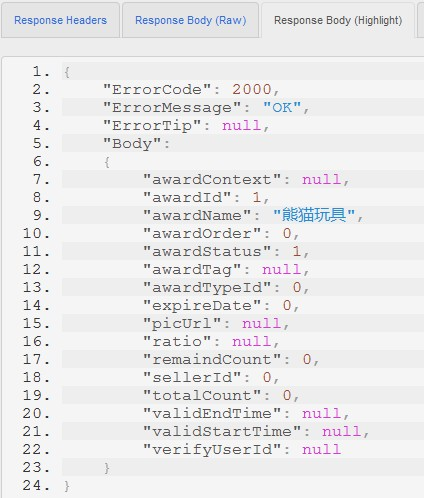
\includegraphics[scale=0.8]{ReturnJsonDemo.jpg}
	\caption{接口数据返回}
	\label{fig:ReturnJsonDemo}
\end{figure}

在RESTful架构中,每个网址代表一种资源(resource),
所以网址中不能有动词,只能有名词,
而且所用的名词往往与数据库的表格名对应。
一般来说,数据库中的表都是同种记录的"集合"(collection),
所以API中的名词也应该使用复数。

\begin{lstlisting}[language=HTML]
https://api.example.com/zoos
\end{lstlisting}

\subsection{WCF测试客户端}

Windows Communication Foundation(WCF)测试客户端(WcfTestClient.exe)是一个 GUI 工具,
使用该工具,用户可以输入测试参数、将该输入提交给服务并查看服务发回的响应。
当与 WCF 服务主机结合时,它可以提供完美的服务测试体验。
the MSDN documentation tells you to navigate to the 

\begin{lstlisting}[language=Bash]
%SystemDrive%\Program Files\Microsoft Visual Studio 10.0\Common7\IDE
\end{lstlisting}

folder. BUT, if you’re running 64-bit Windows, you won’t find it there. You’ll need to look in
\begin{lstlisting}[language=Bash]
%SystemDrive%\Program Files (x86)\Microsoft Visual Studio 10.0\Common7\IDE folder
\end{lstlisting}
 
instead.

\subsection{WCF和Web Service的异同}

WCF is a replacement for all earlier web service technologies from Microsoft. 
It also does a lot more than what is traditionally considered as "web services".

WCF "web services" are part of a much broader spectrum of remote communication enabled through WCF. 
You will get a much higher degree of flexibility and portability doing things in WCF than through 
traditional ASMX because WCF is designed, 
from the ground up, to summarize all of the different distributed programming infrastructures offered by Microsoft.
 An endpoint in WCF can be communicated with just as easily over SOAP/XML as it 
 can over TCP/binary and to change this medium is simply a configuration file mod. 
In theory, this reduces the amount of new code needed when porting or changing business needs, targets, etc.

ASMX is older than WCF, 
and anything ASMX can do so can WCF (and more). 
Basically you can see WCF as trying to logically group together all the different ways of getting two apps to communicate in the world of Microsoft; 
ASMX was just one of these many ways and so is now grouped under the WCF umbrella of capabilities.

Web Services can be accessed only over HTTP \& it works in stateless environment, 
where WCF is flexible because its services can be hosted in different types of applications. 
Common scenarios for hosting WCF services are IIS,WAS, Self-hosting, Managed Windows Service.

The major difference is that Web Services Use XmlSerializer. 
But WCF Uses DataContractSerializer which is better in Performance as compared to XmlSerializer\footnote{具体请参考:
\url{http://www.codeproject.com/Articles/139787/
What-s-the-Difference-between-WCF-and-Web-Services}}.

\subsection{WCF的配置}

WCF配置下主要包含:bindings、Services、behaviors。
behaviors又包含4种behavior:
serviceBehaviors, endpointBehaviors, contractBehaviors和operationBehaviors。
这些behavior接口能作为几乎所有其他扩展功能的入口点,
在实现它们的过程中我们能方便地取得后者(其他扩展功能)的引用。
如果浏览器中通过Get展示返回数据如Json和Xml等,
endpointBehaviors的配置如下代码片段所示。

\begin{lstlisting}[language=XML]
<endpointBehaviors>
	<behavior name="commonEndpoint">
	  <webHttp helpEnabled="true" />
	</behavior>
</endpointBehaviors>
\end{lstlisting}

在项目中可以点击右键弹出菜单,选择"编辑WCF配置",
调取svcConfigEditor.exe程序对WCF的配置进行编辑,
如图\ref{fig:EditWCFConfig}所示。

\begin{figure}[htbp]
	\centering
	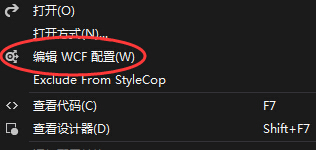
\includegraphics[scale=1]{EditWCFConfig.jpg}
	\caption{编辑WCF配置菜单}
	\label{fig:EditWCFConfig}
\end{figure}

配置在system.serviceModel配置节中,
包含bindings、client。binding的策略选择见图\ref{fig:WCFChoseaBindingStategy}。

\begin{figure}[htbp]
	\centering
	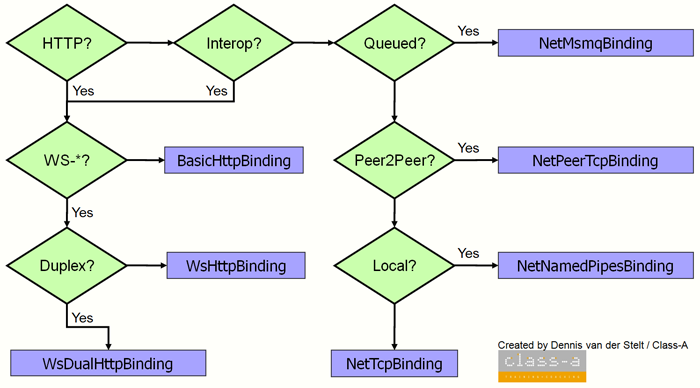
\includegraphics[scale=0.5]{WCFChoseaBindingStategy.png}
	\caption{WCF的binding策略选择}
	\label{fig:WCFChoseaBindingStategy}
\end{figure}

WCF提供了一种特殊的终结点——元数据\footnote{元数据(Metadata),
又称中介数据、中继数据,为描述数据的数据(data about data),
主要是描述数据属性(property)的信息,
用来支持如指示存储位置、历史数据、资源查找、文件记录等功能。
元数据是关于数据的组织、数据域及其关系的信息,
简言之,元数据就是关于数据的数据。}
交换终结点(MEX终结点-Metadata Exchange),
通过它,服务就能够发布元数据。
WCF服务端和客户端通过共享元数据(包括服务协定、服务器终结点信息)在两个终结点上建立通道从而进行通信。
我们通过手写代码(或配置)的方式为服务端编写了元数据信息,
没有借助元数据交换就实现了通信。然而在实际应用中,
元数据往往是很多的,而且重复编写元数据的工作也是不值得的,
因此必然会用到元数据交换的方式让客户端获取元数据。

\subsection{WCF契约}

服务契约定义了远程访问对象和可供调用的方法,
数据契约则是服务端和客户端之间要传送的自定义数据类型。
只有声明为DataContract的类型的对象可以被传送,
且只有成员属性会被传递,成员方法不会被传递。
WCF对声明为DataContract的类型提供更加细节的控制,
可以把一个成员排除在序列化(Serialization)范围以外,也就是说,
客户端程序不会获得被排除在外的成员的任何信息,
包括定义和数据。默认情况下,所有的成员属性都被排除在外,
因此需要把每一个要传送的成员声明为DataMember。
DataContract也支持Name\textbackslash Namespace属性,
如同ServiceContract,Name和Namespace可以自定义名称和命名空间,
客户端将使用自定义的名称和命名空间对DataContract类型进行访问。

\subsection{WCF的调用}

浏览部署完毕后的WCF页面,文件名以svc结尾。
浏览此文件时会有一个网址,形如:\url{http://129.21.11.121:8018/WCFService/Tools/UploadFile.svc?wsdl},
将此网址添加进Visual Studio的Web Service引用即可。
系统在引用后会自动添加形如如下代码的配置并同时创建代理类,
客户端需要一个代理类来访问服务。

\begin{lstlisting}[language=XML]
<system.serviceModel>
    <bindings>
        <basicHttpBinding>
            <binding name="BasicHttpBinding_IUploadFile" messageEncoding="Mtom" />
        </basicHttpBinding>
    </bindings>
    <client>
        <endpoint address="http://129.21.11.121:8018/WCFService/Tools/UploadFile.svc?wsdl"
            binding="basicHttpBinding" bindingConfiguration="BasicHttpBinding_IUploadFile"
            contract="WCFFileService.IUploadFile" name="BasicHttpBinding_IUploadFile" />
    </client>
</system.serviceModel>
\end{lstlisting}

MTOM(Message Transmission Optimization Mechanism)编码\footnote{MTOM(Message Transmission Optimization Mechanism)编码,
MTOM是一种机制,用来以原始字节形式传输包含SOAP消息的较大二进制附件,
从而使所传输的消息较小。
使用MTOM的目的在于优化对较大的二进制负载的传输。
对于较小的二进制负载来说,使用MTOM发送SOAP 消息会产生显著的开销,
但是,当这些负载增大到几千个字节时,
该开销会变得微不足道。
原因在于,正常文本XML使用Base64对二进制数据进行编码,这要求每三个字节对应四个字符,
从而使得数据的大小增加三分之一。MTOM能够以原始字节形式传输二进制数据,
这会缩短编码/解码时间并生成较小的消息。
与当今的业务文档和数字照片相比,几千个字节的阈值是非常小的。},如有必要,
需手动将此段代码拷贝到当前程序正在使用的配置文件中,
绑定(bindings)描述了服务的通信方式,
其中basicHttpBinding用于最广泛的交互操作的第一代Web服务。
所使用的传输协议是HTTP或HTTPS,
安全性由协议保证\footnote{《C\#高级编程》(第三版)第43.5节}。
客户端调用服务如下代码片段\ref{ClientInvokeWcf}所示:

\begin{lstlisting}[language={[Sharp]C},caption=调用WCF接口上传文件,label=ClientInvokeWcf]
#region 上传文件
/// <summary>
/// 上传文件
/// </summary>
/// <param name="extension">文件扩展名</param>
/// <param name="path">服务器保存路径</param>
/// <param name="source">本地路径</param>
/// <param name="inputStream">文件流</param>
public void UploadFileWithFileStream(string extension, string path, string source, Stream inputStream)
{
    try
    {
        UploadFileClient uploadFileClient = new UploadFileClient();
        string fullPath = string.Empty;
        string fileName = string.Empty;
        bool isSuccess = true;
        string errorMesssage = uploadFileClient.StreamToFile(extension, path, inputStream, out fileName, out fullPath, out isSuccess);
        if (!isSuccess)
        {
            logger.Error("Upload file failed!" + errorMesssage);
        }
        uploadFileClient.Close();
    }
    catch (Exception e)
    {
        logger.Error("Upload file failed,path:" + source, e);
    }
}
#endregion
\end{lstlisting}

此种调用方式一般不推荐,此访问操作需要得知访问的具体地址,
加以服务引用即可,不足之处是可能出现序列化失败,值传递异常,
加载资源大,需要生成一堆使用不了的文件,服务端是附加在Web API上的通过配置文件将WCF开放出来。
注意最后调用服务实例的Close方法,将WCF服务的客户端关闭,
否则此连接会在设置的会话(一般为10分钟)后才自动关闭。
期间任何客户端也无法使用此服务。
如果默认的连接数不能满足客户端的需要,可以增加连接数。
配置文件如下:

\begin{lstlisting}
<serviceThrottling maxConcurrentCalls="20" maxConcurrentSessions="20" maxConcurrentInstances="30" />
\end{lstlisting}

说明:maxConcurrentCalls :最大并发数,默认为16;
maxConcurrentSessions :最大的会话数,
主要针对于PerSession的情况,默认为10;
maxConcurrentInstances:最大实例数,默认为26

\subsection{Web Request和ajax调用}

WCF接口需要满足在非.NET客户程序中,可直接调用,
同时在可通过Ajax的Get请求可获取WCF服务返回结果。
满足如上要求之前,需要了解一下RESTful架构\footnote{更早的有RPC(Remote Procedure Call Protocol)
和SOAP(Simple Object Access Protocol)}。
REST\footnote{REST,即Representational State Transfer的缩写。阮一峰对这个词组的翻译是"表现层状态转化"。}这个词,
是Roy Thomas Fielding在他2000年的博士论文中提出的。
什么是RESTful架构:

  (1)每一个URI代表一种资源;

  (2)客户端和服务器之间,传递这种资源的某种表现层;

  (3)客户端通过四个HTTP动词,对服务器端资源进行操作,
实现“表现层状态转化(Representational State Transfer)”。

RESTful架构,就是目前最流行的一种互联网软件架构。
它结构清晰、符合标准、易于理解、扩展方便,跨平台跨语言。
所以正得到越来越多网站的采用\footnote{\url{http://www.ruanyifeng.com/blog/2011/09/restful.html}}。
客户端用到的手段,只能是HTTP协议。具体来说,就是HTTP协议里面,
四个表示操作方式的动词:GET、POST、PUT、DELETE。它们分别对应四种基本操作:
GET用来获取资源,POST用来新建资源(也可以用于更新资源),
PUT用来更新资源,DELETE用来删除资源。
在WCF服务中添加WebGet属性,添加后方法的接口定义:

\begin{lstlisting}[language={[Sharp]C}]
[OperationContract]
[WebGet(UriTemplate = "/GetSellerListByPage/pageIndex={pageIndex}&pageSize={pageSize}&count={count}",
    ResponseFormat = WebMessageFormat.Json,
    BodyStyle = WebMessageBodyStyle.Wrapped)]
List<discount_sellerModel> GetSellerListByPage(int pageIndex, int pageSize, ref int count);
\end{lstlisting}

这里加了一个WebGet的Attribute,
这将允许WCF服务直接通过地址调用。
UriTemplate\footnote{\url{https://msdn.microsoft.com/zh-cn/library/system.uritemplate\%28v=vs.100\%29.aspx}}
是一个表示统一资源标识符 (URI) 模板的类,
继承自Object基类。
接口中一个方法中添加了WebGet之后,
其他方法也需要添加WebGet并将WebMessageBodyStyle设置为Wrapped\footnote{有4个枚举值,
分别为Bare:Both requests and responses are not wrapped.
Wrapped:Both requests and responses are wrapped.
WrappedRequest:Requests are wrapped, responses are not wrapped.
WrappedResponse:Responses are wrapped, requests are not wrapped.}。
请求消息和回复消息分别是对操作方法输入参数和返回值(输出参数和引用参数)的封装,
WebMessageBodyStyle中的Bare表示请求消息和回复消息的主体部分仅仅包含针对输入参数和返回值(输出参数和引用参数)序列化后的内容,
而Wrapped则会在外面包装一个基于当前操作的“封套”。
Bare消息风格返回的Json串可直接在客户端反序列化,
而Wrapped方式返回的Json串需要在客户端定义Model,
这是Bare消息风格的优势。
但是Bare消息主体风格有一些限制,
对于Bare消息主体风格来说,
意味着对象被序列化后生成的XML或者JSON表示直接作为消息的主体,
所以只适用于单一对象。具体来说,
只有具有唯一输入参数的操作方法才能将请求消息的主题风格设置为Bare。

\begin{lstlisting}[language={[Sharp]C}]
[ServiceContract(Namespace = "http://www.artech.com/")]
public interface ICalculator
{
	[WebInvoke(BodyStyle = WebMessageBodyStyle.Bare)]
	double Add( double x,  double y);
}
\end{lstlisting}

如上所示的是我们熟悉的计算服务的契约接口的定义。
消息主体风格为Bare的操作方法Create具有两个输入参数(x和y),
在对实现了该契约接口进行寄宿的时候就会抛出如下图所示的InvalidOperationException异常,
提示“约定“ICalculator”的操作‘Add’指定要序列化多个请求正文参数,
但没有任何包装元素。如果没有包装元素,至多可序列化一个正文参数。
请删除多余的正文参数,
或将WebGetAttribute/WebInvokeAttribute的BodyStyle属性设置为Wrapped。
由于回复参数是对返回值、引用参数和输出参数的封装,
所以\emph{当操作方法具有引用参数(ref关键字)或者输出参数(out关键字)时不能将回复消息的主体风格设置为Bare}。

\begin{lstlisting}[language={[Sharp]C}]
[ServiceContract(Namespace = "http://www.artech.com/")]
public interface ICalculator
{
	[WebInvoke(BodyStyle = WebMessageBodyStyle.WrappedRequest)]
	void Add(double x, double y, out double result);
}
\end{lstlisting}

同样以计算服务契约为例,现在我们通过如上的方式以输出参数的形式返回加法运算的结果,
并将应用在操作方法上的WebInvokeAttribute特性的BodyStyle属性设置为WrappedRequest,
这意味着请求消息和回复消息分别采用Wrapped和Bare风格。
当我们对实现了该契约接口的服务设施寄宿时会抛出下图所示的InvalidOperationException异常,
并提示“约定‘ICalculator’的操作‘Add’至少指定一个响应正文参数不是操作的返回值。
当WebGetAttribute/WebInvokeAttribute的BodyStyle属性设置为Bare 时,
只允许使用返回值。请删除多余的响应正文参数或将BodyStyle属性设置为 Wrapped”。
pageIndex等加中括号的内容代表在提交Get请求时传入的参数,
参数之间用符号\&进行分隔。修改配置文件为:

\begin{lstlisting}[language=XML]
<system.serviceModel>
<services>
 <service behaviorConfiguration="RR.API.WCFService.User.UserServiceBehavior"
  name="RR.API.WCFService.User.UserService">
  <endpoint address="" binding="webHttpBinding" contract="RR.API.WCFService.User.IUserService" behaviorConfiguration="test" bindingConfiguration="basicWeb">
   <identity>
    <dns value="localhost" />
   </identity>
  </endpoint>
  <endpoint address="mex" binding="mexHttpBinding" contract="IMetadataExchange" />
 </service>
</services>

<bindings>
  <basicHttpBinding>
      <binding closeTimeout="00:10:00" receiveTimeout="00:20:00" sendTimeout="00:20:00" maxBufferSize="20000000" maxReceivedMessageSize="20000000">
      <security mode="None"></security>
    </binding>
  </basicHttpBinding>
  <webHttpBinding>
    <binding name="basicWeb"/>
  </webHttpBinding>
</bindings>

<behaviors>
  <serviceBehaviors>
    <behavior name="RR.API.WCFService.User.UserServiceBehavior">          
        <serviceMetadata httpGetEnabled="true"/>
        <serviceDebug includeExceptionDetailInFaults="false"/>
      </behavior>
  </serviceBehaviors>
  
  <endpointBehaviors>
    <behavior name="test">
      <webHttp/>
   </behavior>
 </endpointBehaviors>
</behaviors>
<serviceHostingEnvironment multipleSiteBindingsEnabled="true" />
</system.serviceModel>
\end{lstlisting}

WebHttpBinding用于通过HTTP请求提供的服务,
它对于脚本客户端很有用,
如ASP.NET AJAX\footnote{<C\#高级编程>43.5节}.在WCF实际运行的过程中,访问的地址以配置文件配置的地址为准,
和实际引用的地址无关。配置完毕后在浏览器中输入形如如下链接:

\begin{lstlisting}[language=XML]
http://129.11.21.18:8019/WCFService/Product/PublicProductService.svc/
GetSingleSellerAwardListByPage?pageIndex={PAGEINDEX}&pageSize={PAGESIZE}&count={COUNT}&sellerId={SELLERID}
\end{lstlisting}

将会看到访问后的结果。
将Web.config中的 <webHttp/> 修改为 <webHttp helpEnabled="true"/>将可以在浏览器页面中列举出可用接口,
并提供提交的数据样例。打开浏览器,
在地址栏输入\url{http://IP:Port/Services/ShowerService.svc/help}即可,
如图\ref{fig:WCFInterfaceHelpPage}所示。

\begin{figure}[htbp]
	\centering
	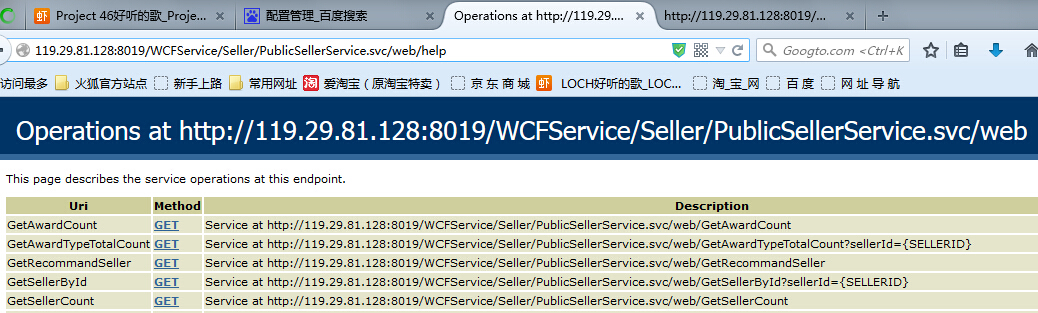
\includegraphics[scale=0.6]{WCFInterfaceHelpPage.jpg}
	\caption{查看WCF可用接口}
	\label{fig:WCFInterfaceHelpPage}
\end{figure}

因为REST是基于HTTP的,所以对于REST的客户端的开发者,
无法像传统的 WebService或者其他的WCF服务通过引用WSDL,
享受“奢侈”的代码生成,而使用强类型的本地代理调用服务。 
开发者只能通过Http Request的组装, 
但正因为这种直接的HttpRequest组装,而使得客户端真正是语言无关的。
WCF通过Web调用时,所用的绑定方式是webHttpBinding。
通过客户端引用方式调用时,所用的绑定方式是basicHttpBinding。
在service配置节下添加不同的终节点(endpoint),
针对Web调用,终节点的配置如代码片段\ref{WebInvokeEndpointConfig}所示。

\begin{lstlisting}[language=XML,caption=Web调用的终节点配置,label=WebInvokeEndpointConfig]
<endpoint address="web" behaviorConfiguration="commonEndpoint" binding="webHttpBinding" contract="RR.API.WCFService.Custom.IPublicBaseService"/>
\end{lstlisting}

在web调用时用如\url{http://localhost:50590/WCFService/Custom/PublicBaseService.svc/web/DoWork?a={A}}形式的Url。
同样在浏览器查看所有可用接口集合的时候也需要在Url中包含终节点地址名称,
形如\url{http://localhost:50590/WCFService/Custom/PublicBaseService.svc/web/help},
其中web为终节点地址的名称。而通过客户端调用的还是原来的终节点配置,
如代码\ref{RefernceInvokeEndpointConfig}所示。

\begin{lstlisting}[language=XML,caption=客户端引用调用service终节点配置,label=RefernceInvokeEndpointConfig]
<endpoint binding="basicHttpBinding"  contract="RR.API.WCFService.Custom.IPublicBaseService"></endpoint>
\end{lstlisting}

通过Http Request方式调用的链接和客户端引用方式调用的链接是不一样的,
Http Request方式调用的Url中需要加上endpoint的Address名称。
通过Http Request而不通过引用的方式调用,
是因为引用的方式调用会在客户端生成大量代码,
自动生成许多文件,
给维护造成困难。
另WCF的参数只有一个时,可写成如图\ref{fig:WCFParamStyle}所示的形式。

\begin{figure}[htbp]
	\centering
	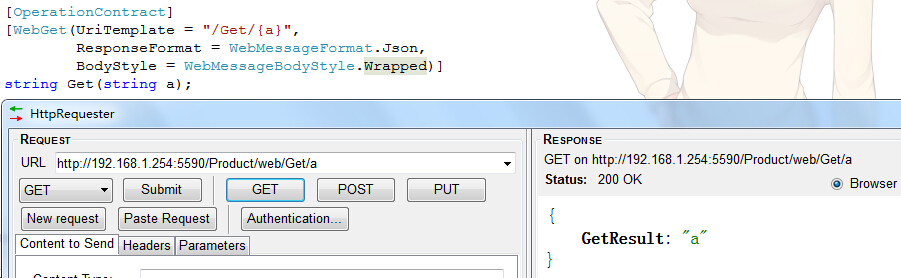
\includegraphics[scale=0.6]{WCFParamStyle.jpg}
	\caption{WCF的Url参数风格}
	\label{fig:WCFParamStyle}
\end{figure}

\subsection{WCF REST AJax跨域请求调用}

网络应用程序,分为前端和后端两个部分。
当前的发展趋势,就是前端设备层出不穷(手机、平板、桌面电脑、其他专用设备......)。
因此,必须有一种统一的机制,
方便不同的前端设备与后端进行通信。
这导致API构架的流行,甚至出现"API First"的设计思想。
RESTful API是目前比较成熟的一套互联网应用程序的API设计理论\cite{RESTful API设计指南}。
在以前,前端和后端混杂在一起,比如JavaScript直接调用同系统里面的一个Httphandler,
就不存在跨域的问题,但是随着现代的这种多种客户端的流行,
比如一个应用通常会有Web端,App端,
以及WebApp端,各种客户端通常会使用同一套的后台处理逻辑,
即API,前后端分离的开发策略流行起来,
前端只关注展现,通常使用JavaScript,
后端处理逻辑和数据通常使用WebService来提供json数据。
一般的前端页面和后端的WebService API通常部署在不同的服务器或者域名上。
这样,通过ajax请求WebService的时候,就会出现同源策略的问题。

传统的Ajax请求只能获取在同一个域名下面的资源,
即只有协议+主机名+端口号 (如存在)相同,则允许相互访问。
也就是说JavaScript只能访问和操作自己域下的资源,
不能访问和操作其他域下的资源。
但是HTML5打破了这个限制,允许Ajax发起跨域的请求。
浏览器是可以发起跨域请求的,比如你可以外链一个外域的图片或者脚本。
但是Javascript脚本是不能获取这些资源的内容的,
它只能被浏览器执行或渲染。
AJax支持跨域的解决方案目前就是JSONP(JSON with Padding)。
在使用用AJax调用接口时出现如下提示:

\begin{lstlisting}
同源策略禁止读取位于http://129.29.1.28:8019/Product/web/Get?{%20%22a%22:%20%22a%22%20}&_=1441558531991 的远程资源。(原因:CORS 头缺少 'Access-Control-Allow-Origin')。
\end{lstlisting}

正常使用AJax会需要正常考虑跨域问题,
所以伟大的程序员们又折腾出了一系列跨域问题的解决方案,
如JSONP、flash、ifame、xhr2等等。
CORS定义一种跨域访问的机制,可以让AJax实现跨域访问。
CORS允许一个域上的网络应用向另一个域提交跨域AJax请求。
实现此功能非常简单,只需由服务器发送一个响应标头即可。
一个域是由schema、host、port三者共同组成,与路径无关。

所谓跨域,是指在http://example-foo.com/域上通过XMLHttpRequest对象调用http://example-bar.com/域上的资源。
CORS约定服务器端和浏览器在HTTP协议之上,通过一些额外HTTP头部信息,进行跨域资源共享的协商。
服务器端和浏览器都必需遵循规范中的要求。

\subsubsection{使用CROS实现AJax跨域访问}

CORS(跨域资源共享,Cross-Origin Resource Sharing)定义一种跨域访问的机制,
可以让AJax实现跨域访问。
CORS允许一个域上的网络应用向另一个域提交跨域AJax请求。
实现此功能非常简单,只需由服务器发送一个响应标头即可。
跨域资源共享CORS与JSONP相比,
无疑更为先进、方便和可靠。

\begin{enumerate}
\setcounter{enumi}{0}
\item{JSONP只能实现GET请求,而CORS支持所有类型的HTTP请求。}
\item{使用CORS,开发者可以使用普通的XMLHttpRequest发起请求和获得数据,比起JSONP有更好的错误处理。}
\item{JSONP主要被老的浏览器支持,它们往往不支持CORS,而绝大多数现代浏览器都已经支持了CORS}
\end{enumerate}      

CORS需要浏览器和服务器同时支持。目前,所有浏览器都支持该功能,IE浏览器不能低于IE10。
整个CORS通信过程,都是浏览器自动完成,不需要用户参与。对于开发者来说,
CORS通信与同源的AJAX通信没有差别,代码完全一样。浏览器一旦发现AJAX请求跨源,
就会自动添加一些附加的头信息,有时还会多出一次附加的请求,但用户不会有感觉。
因此,实现CORS通信的关键是服务器。只要服务器实现了CORS接口,就可以跨源通信。
For WCF service you have to develop new behavior and include it in the endpoint configuration\footnote{http://enable-cors.org/server\_wcf.html}: 


客户端脚本如下所示:

\begin{lstlisting}[language=HTML]
<center style="margin-bottom:20px">
    <a class="btn btn-block btn-lg btn-warning" id="input-verifycros">CROS实现WCF跨域调用</a>
    <div id="content"></div>
</center>
\end{lstlisting}

调用服务的AJax脚本:

\begin{lstlisting}[language=VBScript]
var xmlHttpRequest=new XMLHttpRequest();
$(function () {
    $("#input-verifycros").bind("click", function () {               
        //http://127.0.0.1:5509/my/WCFAJaxTest
        var url = "http://129.19.1.138:7019/WCFService/Custom/ServiceCros.svc/web/DoWork/a";                
        if (xmlHttpRequest) {
            xmlHttpRequest.open('GET', url, true);
            xmlHttpRequest.onreadystatechange = handler;
            xmlHttpRequest.send();
        }
        else {
            document.getElementById("content").innerHTML = "不能创建XMLHttpRequest";
        }
    })
});
\end{lstlisting}

XMLHttpRequest是AJax的基础,
所有现代浏览器(IE7+、Firefox、Chrome、Safari 以及Opera)均内建XMLHttpRequest对象。
每当readyState改变时,就会触发onreadystatechange事件。
readyState属性存有XMLHttpRequest的状态信息。
存有XMLHttpRequest的状态,从0到4发生变化:

0: 请求未初始化

1: 服务器连接已建立

2: 请求已接收

3: 请求处理中

4: 请求已完成,且响应已就绪

open方法规定请求的类型、URL以及是否异步处理请求。
脚本HttpRequest调用的函数:

\begin{lstlisting}[language=VBScript]
function handler(evtXHR) {  
    if (xmlHttpRequest.readyState == 4) {                
        console.log("HTTP status:" + xmlHttpRequest.status);
        if (xmlHttpRequest.status == 200) {
            var response = xmlHttpRequest.responseText;                    
            document.getElementById("content").innerHTML = "结果:" + response;
        } else {
            console.log("不允许跨域请求");
            document.getElementById("content").innerHTML = "不允许跨域请求。";
        }
    }
    else {                
        document.getElementById("content").innerHTML += "<br/>执行状态 readyState:" + xmlHttpRequest.readyState;
    }
}
\end{lstlisting}

参考链接\footnote{http://debugmode.net/2014/06/12/solved-access-control-allow-origin-error-in-wcf-rest-service/}。
服务端的配置Step 1:

\begin{lstlisting}[language=XML]
<system.webServer>
	<httpProtocol>
		<customHeaders>
			<add name="Access-Control-Allow-Origin" value="*" />
		</customHeaders>
	</httpProtocol>    
	
	<modules runAllManagedModulesForAllRequests="true"/>  
	<directoryBrowse enabled="true"/>
</system.webServer>
\end{lstlisting}

服务端的配置Step 2:在system.serviceModel 中的standardEndpoint增加配置。

\begin{lstlisting}[language=XML]
<standardEndpoints>
  <webHttpEndpoint>
    <standardEndpoint crossDomainScriptAccessEnabled="true"/>
  </webHttpEndpoint>
</standardEndpoints>
\end{lstlisting}


\subsubsection{使用JSONP实现AJax跨域访问}

同源策略下,某个服务器是无法获取到服务器以外的数据,
但是html里面的img,iframe和script等标签是个例外,
这些标签可以通过src属性请求到其他服务器上的数据。
而JSONP就是通过script节点src调用跨域的请求。
在WCF REST中使用AJax跨域请求调用WCF接口需要在服务端配置,
同时在客户端调用时需要使用jsonp的方式。
服务端的配置如下代码所示\footnote{http://www.cnblogs.com/artech/archive/2012/01/16/jsonp-wcf-rest.html}:

\begin{lstlisting}[language=HTML]
<standardEndpoints>
	<webHttpEndpoint>
	<standardEndpoint crossDomainScriptAccessEnabled="true"/>
	</webHttpEndpoint>
</standardEndpoints>
<bindings>
	<webHttpBinding>
	<binding crossDomainScriptAccessEnabled="true" />
	</webHttpBinding>
</bindings>
\end{lstlisting}

同时在服务的相应终结点上添加kind属性,
如下例子所示:

\begin{lstlisting}[language=HTML]
<services>  
	<service name="Artech.WcfServices.Service.EmployeesService">
		<endpoint kind="webHttpEndpoint" 
	         	  address="http://127.0.0.1:3721/employees"
	       		  contract="Artech.WcfServices.Service.Interface.IEmployees"/>
	</service>
</services>
\end{lstlisting}

客户端调用代码如下所示:

\begin{lstlisting}[language=VBScript]
<script>
    $(function () {
        $("#input-verify").bind("click", function () {                 
            //http://192.168.1.254:5508/my/WCFAJaxTest
            var url = "http://129.9.1.138:8019/Product/web/Get/a";
            jQuery.ajax({                    
                url: url,                                       
                type: 'get',                    
                dataType: 'jsonp', 
                success: function (data) {                        
                    alert(data);                          
                },
                error: function (xhr, status, error) {
                    console.log(xhr);
                    if (xhr == 'undefined' || xhr == undefined) {
                        alert('undefined');
                    } else {
                        alert('object is there');
                    }
                    alert(status);
                    alert(error);
                }
            });
        })
    });
</script>
\end{lstlisting}

为了避免与NVelocity模板冲突,
此处使用jQuery.ajax的写法,
另一种写法为\$.ajax,两种写法没有本质的区别,
\$即是Jquery的简写,\$只是jquery的代表符号,
只有引入jquery.js后才可以这么用它,
\$.ajax其实用的是jQuery.ajax。
在jQuery的源码里面有如下语句:

\begin{lstlisting}[language=VBScript]
//Expose jQuery to the global object
window.jQuery = window.$ = jQuery;
\end{lstlisting}

许多JavaScript库使用\$作为函数或变量名,jQuery也一样。
在jQuery中,\$仅仅是jQuery的别名,
因此即使不使用\$也能保证所有功能性。
比如你想要将jQuery嵌入一个高度冲突的环境,
假如我们需要使用jQuery之外的另一JavaScript库,
我们可以通过调用\$.noConflict()向该库返回控制权。

需要注意的是在进行Ajax调用的使用将dataType选项设置成“jsonp”,
而不是“json”,这是关键的地方。console.log原先是Firefox 的“专利”,
严格说是安装了Firebugs之后的Firefox所独有的调试“绝招”。
这一招,IE8学会了,不过用起来比Firebug麻烦,
只有在开启调试窗口(F12)的时候,console.log才能出结果,不然就报错。
console.log(),可以用来取代alert()或document.write()。
比如,在网页脚本中使用console.log("Hello World"),
加载时控制台就会自动显示如下内容。

\subsection{WCF RESTful接口传输文件}

一般情况下文件传输有如下4种方式。

\subsubsection{Base64 byte[]}
一般来说,最简单的方式就是利用byte[]作为数据类型来设计你的Web Service。
byte[]无论是作为一个简单参数或者你的一个自定义对象的成员变量都可以。

客户端把文件内容全部读出,填入一个byte[],
然后经过base64的encode(这个工作一般由Web Service框架来完成),
然后发送给服务端,服务端先经过base64的decode(同样,一般由框架完成),
然后应用程序就可以拿到byte[]了。

这个方法比较简单,但是其问题也不小,就是不适合传输大文件。
原因base64加密后的byte[]实际上是作为SOAP报文XML的一部分的,
其字节数大约比加密前的字节数多三分之一。
要命的是这些内容会被全部整体读入内存(因为XML报文解析),
如果文件很大,那么内存的占用就很厉害,
想象系统一般是多用户共用的,是不是很容易闹出OOM(Out of Memory)的问题?

\subsubsection{SOAP Attachments}

类似Email的附件,SOAP也可以采用类似的方式添加附件,
即二进制的文件保持不变,不需要改变编码方式以迁就XML,
其内容不出现在SOAP的XML报文中。
不过这种方式下对编程人员有点麻烦,你需要用SAAJ编程API来操作AttachmentPart。

\subsubsection{MTOM}

结合以上两种方式的优点,既可以保持二进制形式的文件内容,
又保持相对简单的编程模式。
 然而,值得注意的是MTOM和SOAP Attachments这两种方式对大文件都也存在内存问题,
 即大文件的内容字节bytes也是在内存中存放着的,
 如果文件很大,很容易出OOM(Out of Memory)的问题.

\subsubsection{Streaming Mode}

顾名思义,Streaming Mode就是流模式,对于大文件而言,
其内容并不整体保存在内存中,系统拿到一小撮数据后交给应用层,
应用程序把这小撮数据保存到文件中或者作另外的处理,
然后再跟系统要下一小撮数据。。。如此往复,直至所有数据处理完毕。
这种模式是对付大文件,避免OOM(Out of Memory)问题的最好的手段。

WCF上传文件代码。

\begin{lstlisting}[language={[Sharp]C}]
/// <summary>
/// WCF REST接口传输文件
/// </summary>
/// <param name="url">WCF REST链接地址</param>
/// <param name="fileFullLocalPath">上传文件在本地的全路径</param>
public virtual string RESTUpload(string url, string fileFullLocalPath)
{
    string jsonResult = string.Empty;
    try
    {
        HttpClient httpClient = new HttpClient();
        HttpContent httpConent = HttpContent.Create(File.OpenRead(fileFullLocalPath));
        HttpResponseMessage httpResponse = httpClient.Post(url, httpConent);
        httpResponse.EnsureStatusIsSuccessful();
        jsonResult = httpResponse.Content.ReadAsString();
    }
    catch (Exception e)
    {
        logger.Error("Upload failed!", e);
    }
    return jsonResult;
}
\end{lstlisting}

服务端代码如下所示。

\begin{lstlisting}[language={[Sharp]C}]
[OperationContract]
[WebInvoke(Method="POST",
           UriTemplate = "UploadJpegImage",
           BodyStyle = WebMessageBodyStyle.Wrapped,
           ResponseFormat = WebMessageFormat.Json)]
JpegFileInfoResult UploadJpegImage(Stream fileStream);

/// <summary>
/// 保存文件
/// </summary>
/// <param name="fileStream">文件流</param>
public JpegFileInfoResult UploadJpegImage(Stream fileStream)
{
    JpegFileInfoResult jpegFileInfoResult = null;
    JpegFileInfo jpegFileInfo = null;
    var storePath = string.Empty;
    var fileFullName = string.Empty;
    try
    {
        if (System.Web.HttpContext.Current != null)
        {
            storePath = System.Web.HttpContext.Current.Server.MapPath("~/upload/");
        }
        else
        {
            storePath = Path.Combine(HttpRuntime.AppDomainAppPath, "\\upload\\");
        }
        if (!Directory.Exists(storePath))
        {
            Directory.CreateDirectory(storePath);
        }
        string filename = System.Guid.NewGuid().ToString() + ".jpeg";
        fileFullName = Path.Combine(storePath, filename);
        var bitmap = Bitmap.FromStream(fileStream);
        bitmap.Save(fileFullName);        
    }
    catch (Exception e)
    {
        logger.Error("WCF receive image encount an error,fullpath:" + fileFullName, e);        
    }
    return jpegFileInfoResult;
}
\end{lstlisting}


\subsection{WebGet和WebInvoke}

WebInvoke allows you to specify which verb will be allowed, 
defaulting to POST. WebGet requires the client to be using a GET request.
 In either case, if the wrong verb is used, you'll get "method is not allowed". 
 You were using the browser, so it was making a GET request, 
 so a normal POST-only WebInvoke would reject it, whereas a WebGet would allow it. 
 You could specify Method="GET" in the WebInvoke attribute declaration to allow GET, of course.

 WebInvokeAttribute 会确定服务操作响应的 HTTP 方法。
 默认情况下,所有已应用WebInvokeAttribute 的方法都会响应POST请求。
 Method属性允许您指定不同的HTTP方法。如果您希望服务操作响应GET,请改用WebGetAttribute。

\subsection{WCF开启日志}

在开发过程中需要诊断WCF各种未知问题,
日志是最好的帮助,在Configuration中插入以下节点,WCF中客户端开启日志的配置如下。

\begin{lstlisting}[language=HTML]
<system.diagnostics>
    <sources>
        <source name="System.ServiceModel.MessageLogging" switchValue="Warning, ActivityTracing">
            <listeners>
                <add type="System.Diagnostics.DefaultTraceListener" name="Default">
                    <filter type="" />
                </add>
                <add name="ServiceModelMessageLoggingListener">
                    <filter type="" />
                </add>
            </listeners>
        </source>
        <source name="System.ServiceModel" switchValue="Warning, ActivityTracing"
          propagateActivity="true">
            <listeners>
                <add type="System.Diagnostics.DefaultTraceListener" name="Default">
                    <filter type="" />
                </add>
                <add name="ServiceModelTraceListener">
                    <filter type="" />
                </add>
            </listeners>
        </source>
    </sources>
    <sharedListeners>
        <add initializeData="app_messages.svclog"
          type="System.Diagnostics.XmlWriterTraceListener, System, Version=2.0.0.0, Culture=neutral, PublicKeyToken=b77a5c561934e089"
          name="ServiceModelMessageLoggingListener" traceOutputOptions="Timestamp">
            <filter type="" />
        </add>
        <add initializeData="app_tracelog.svclog"
          type="System.Diagnostics.XmlWriterTraceListener, System, Version=2.0.0.0, Culture=neutral, PublicKeyToken=b77a5c561934e089"
          name="ServiceModelTraceListener" traceOutputOptions="Timestamp">
            <filter type="" />
        </add>
    </sharedListeners>
    <trace autoflush="true" />
</system.diagnostics>
\end{lstlisting}

在System.serviceModel 中插入以下节点,如代码片段\ref{WCFLogServiceModelConfig}所示。

\begin{lstlisting}[language=XML,caption=WCF日志serviceModel节点配置,label=WCFLogServiceModelConfig]
<diagnostics wmiProviderEnabled="true" performanceCounters="All">
  <messageLogging logMalformedMessages="true" logMessagesAtTransportLevel="true" />
</diagnostics>
\end{lstlisting}

配置生效后会在程序的目录下生成app\_messages.svclog和app\_tracelog.svclog两个文件.


\subsection{WCF引用安全}

WCF的安全体系主要包括三个方面:
传输安全(Transfer Security)、 授权或者访问控制(Authorization OR Access Control)以及审核(Auditing)。
而传输安全又包括两个方面:认证(Authentication)和消息保护(Message Protection)。
认证帮助客户端或者服务确认对方的真实身份,而消息保护则通过签名和加密实现消息的一致性和机密性。
WCF采用两种不同的机制来解决这三个涉及到传输安全的问题,我们一般将它们称为不同的安全模式,
即Transport安全模式和Message安全模式。
Windows Communication Foundation(WCF)是Microsoft为构建面向服务的应用程序而提供的统一编程模型,
WCF访问权限控制可采用\emph{自定义用户名密码}的验证方式。
WCF提供了如下三种方式来验证凭证中用户名是否和密码相符:

\begin{itemize}
\item{\emph{Windows}:将用户名和密码映射为Windows帐号和密码,采用Windows认证;}
\item{\emph{MembershipProvider}:利用配置的MembershipProvider验证用户名和密码;}
\item{\emph{自定义}:通过继承抽象类UsernamePasswordValidator,自定义用户名/密码验证器进行验证。}
\end{itemize}

WCF支持多种认证技术,
例如Windowns认证、X509证书、Issued Tokens、自定义用户名密码认证等,
在跨Windows域分布的系统中,用户名密码认证还是比较常用的,要实现用户名密码认证,
就必须需要X509证书,为什么呢?
因为我们需要X509证书这种非对称密钥技术来实现WCF在Message传递过程中的加密和解密,
要不然用户名和密码就得在网络上明文传递!
详细说明就是客户端把用户名和密码用公钥加密后传递给服务器端,
当然,做个测试程序就没有必要去申请一个X509数字签名证书了,
微软提供了一个makecert.exe的命令专门用来生成测试使用的X509证书的,
那我们就来建立一个测试用的证书,在cmd下输入以下命令: 

\begin{lstlisting}
C:\Program Files (x86)\Windows Kits\8.1\bin\x64>makecert.exe -sr currentUser -ss
 My -a sha1 -n CN=WCFCertServer -sky exchange -pe //服务端证书
 
C:\Program Files (x86)\Windows Kits\8.1\bin\x64>makecert.exe -sr currentUser -ss
 My -a sha1 -n CN=WCFCertClient -sky exchange -pe //客户端证书
\end{lstlisting}

makecert.exe程序存放在C:\textbackslash Program Files (x86) \textbackslash Windows Kits\textbackslash 8.1\textbackslash bin\textbackslash x64路径下,
证书创建完毕后通过mmc(Microsoft Manager Control)命令打开控制台界面可看到证书,
如图\ref{fig:X509CertForWCF}所示。

\begin{figure}[htbp]
	\centering
	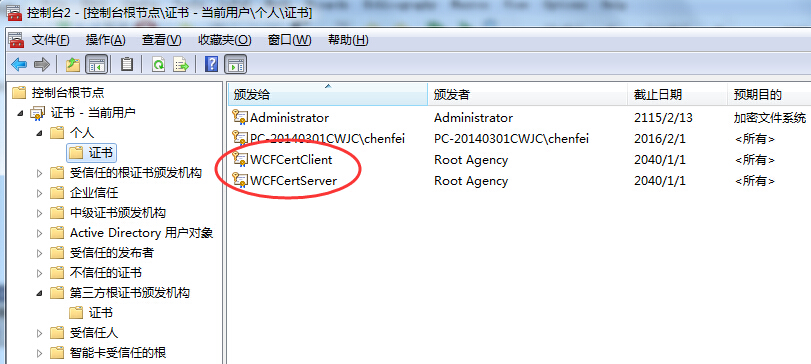
\includegraphics[scale=0.6]{X509CertForWCF.jpg}
	\caption{创建X.509证书}
	\label{fig:X509CertForWCF}
\end{figure}

-sr参数指定的证书存储区中的注册表位置。
为currentUser时指定注册版存储位置为 HKEY\_CURRENT\_USER.
为localMachine时指定注册版存储位置为 HKEY\_LOCAL\_MACHINE.
在访问WCF时若出现\emph{无法使用以下搜索标准找到 X.509 证书: StoreName“My”、StoreLocation“LocalMachine”、FindType“FindBySubjectName”、FindValue“jirisoft”}
或者\emph{密钥集不存在}错误时,是由于没有给读取证书的权限,如图\ref{fig:X509ManagerPrivateKey}所示。

\begin{figure}[htbp]
	\centering
	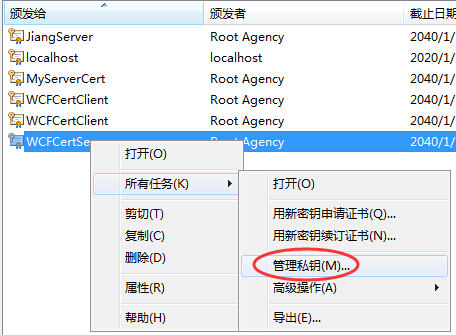
\includegraphics[scale=0.6]{X509ManagerPrivateKey.jpg}
	\caption{管理X.509证书私钥}
	\label{fig:X509ManagerPrivateKey}
\end{figure}

给Everyone账户添加读取的权限即可,
管理证书的菜单只有证书所属为LocalMachine时才有。
服务器端再用自己的私钥来解密,然后传递给相应的验证程序来实现身份验证。 

C:\textbackslash WINDOWS\textbackslash microsoft.net\textbackslash Framework64\textbackslash v4.0.30319

认证所需的数据表\ref{fig:AspNetCredentialTable}如图所示。

\begin{figure}[htbp]
	\centering
	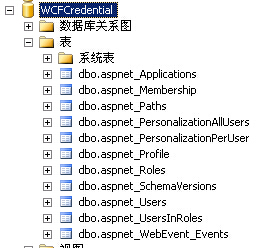
\includegraphics[scale=1]{AspNetCredentialTable.jpg}
	\caption{WCF认证创建的数据表}
	\label{fig:AspNetCredentialTable}
\end{figure}

在配置文件中添加数据库连接串:

\begin{lstlisting}
<add name="WCFCredential" connectionString="Data Source=129.39.1.138,5002;Uid=WCFCredential;Pwd=WCFCredential!@#321;database=WCFCredential"/>
\end{lstlisting}

如果你有一个真正的X509证书,那么现在的代码就可以正常运行了。
但是很不幸,我们的证书是测试用的,
我们运行的时候出错:\emph{ X.509 certificate CN=MyServerCert 链生成失败。
所使用的证书具有无法验证的信任链。
请替换该证书或更改 certificateValidationMode。已处理证书链,
但是在不受信任提供程序信任的根证书中终止',WCF无法验证测试证书的信任链。}
那我们要做的就是绕过这个信任验证,具体做法如下:

\paragraph{WCF安全之自定义Windows验证}

应该说就采用的频率程度,
集成Windows认证(IWA:Integrated Windows Authentication)是仅次于用户名/密码的认证方式。
尤其是在基于Windows活动目录(AD:Active Directory)的Intranet应用来说,
Windows认证更是成为首选。微软几乎所有需要进行认证的产品或者开发平台都集成了Windows认证,
比如IIS,SQL Server,ASP.NET等,当然,WCF也不可能例外。
基于Windows的身份验证服务端的endpoint配置如下:

\begin{lstlisting}
<service behaviorConfiguration="CertificateBehavior" name="RR.API.WCFService.Custom.Service1">
        <endpoint behaviorConfiguration="" 
                  binding="wsHttpBinding" 
                  bindingConfiguration="CertificateBinding" 
                  name="Service1EndPoint" 
                  contract="RR.API.WCFService.Custom.IService1" />
      </service>
\end{lstlisting}

behavior配置如下:

\begin{lstlisting}
 <behavior name="CertificateBehavior">
  <serviceMetadata httpGetEnabled="true" httpGetBinding="webHttpBinding"
    httpGetBindingConfiguration="" />
  <serviceDebug />
  <serviceCredentials>
    <serviceCertificate findValue="WCFCert1" storeLocation="LocalMachine"
      x509FindType="FindBySubjectName" />
  </serviceCredentials>
</behavior>
\end{lstlisting}

binding的配置如下:

\begin{lstlisting}
<wsHttpBinding>
	<binding name="CertificateBinding" messageEncoding="Mtom">
	  <security>
	    <transport clientCredentialType="None" />
	    <message clientCredentialType="UserName" negotiateServiceCredential="false"/>
	  </security>
	</binding>
</wsHttpBinding>
\end{lstlisting}


基于Windows的身份验证客户端的endpoint配置如下:

\begin{lstlisting}
<endpoint address="http://192.168.1.254:5590/WCFService/Custom/Service1.svc"
        binding="wsHttpBinding"
        bindingConfiguration="Service1EndPoint"
        behaviorConfiguration="CertificateBehavior"
        contract="WCFValidateService.IService1"
        name="Service1EndPoint">
<identity>
  <certificate encodedValue="AwAAAAEAAAAUAAAABMqx3Nytjb4g0X+WAefU5NwHH10gAAAA
  AQAAADgCAAAwggI0MIIB4qADAgECAhCMdbkl4fDgqkppsNbqOzC2MAkGBSsOAwIdBQAwFjEUMBI
  GA1UEAxMLUm9vdCBBZ2VuY3kwHhcNMTUwODA2MDkwNDUxWhcNMzkxMjMxMjM1OTU5WjATMREwDw
  YDVQQDEwhXQ0ZDZXJ0MTCCASIwDQYJKoZIhvcNAQEBBQADggEPADCCAQoCggEBALM0Fmjkx88RP
  JUcGAdL0UBA2yB0/FiICDDHEagjCvK0RWXsa+ha0N30EjZ5Nqvd9jtqOxb2fgm/lFbyP23MaCp2
  mL9McV7AFftu3m1/betkskUHZD5y/EUGzXFwyhGFezD5o6BFjn8zlcQYjU8aRIyFpQf0MeCO62Z
  tUd/92CyCsuzt8xsIXMm63i2yV46RhU5vObgB/D40FVHuJUBbbrDYmRVqaUjIS2yq9DiX5+7oim
  vz9CHQp6r3vnnZ3pW8xcwE3zL/xEUNP+zs6ZLuOF/ad0SNYrDa0+BYAQlFUVJfiZz35larGLDzd
  ikqty4kJxHf7W/CxbiSaXMOgb2Fq8MCAwEAAaNLMEkwRwYDVR0BBEAwPoAQEuQJLQYdHU8AjWEh
  3BZkY6EYMBYxFDASBgNVBAMTC1Jvb3QgQWdlbmN5ghAGN2wAqgBkihHPuNSqXDX0MAkGBSsOAwI
  dBQADQQAuCvXzvzI7Ec+VeU89Z09AKuLL9M5cEPUmr140z6l5FaqyIbA9LzvFp/nQ7fu1cPjK6C
  OcqWWlk6vTolLPWK8R" />
</identity>
</endpoint>
\end{lstlisting}


bindings配置如下。

\begin{lstlisting}
<wsHttpBinding>
	<binding name="Service1EndPoint" messageEncoding="Mtom">
	  <security>
	    <message clientCredentialType="UserName" negotiateServiceCredential="false" />
	  </security>
	</binding>
</wsHttpBinding>
\end{lstlisting}

behavior的配置如下。

\begin{lstlisting}
<behavior name="CertificateBehavior">
  <clientCredentials>
    <clientCertificate findValue="WCFCert1" storeLocation="LocalMachine"
      x509FindType="FindBySubjectName" />
    <serviceCertificate>
      <defaultCertificate findValue="WCFCert1" storeLocation="LocalMachine"
        x509FindType="FindBySubjectName" />
      <authentication certificateValidationMode="None" trustedStoreLocation="LocalMachine" />
    </serviceCertificate>
  </clientCredentials>
</behavior>
\end{lstlisting}

采用Windows用户名密码认证的调用方式如代码所示。

\begin{lstlisting}[language={[Sharp]C},caption=认证方式调用WCF接口,label=CertificateInvokeWCF]
Service1Client service1Client = new Service1Client();
service1Client.ClientCredentials.UserName.UserName = "Administrator";
service1Client.ClientCredentials.UserName.Password = "123";
string returnValue = service1Client.GetData(100);
service1Client.Close();
\end{lstlisting}

其中Administrator为登录Windows的用户名,
123为登录Windows的密码。

\paragraph{WCF安全之自定义身份验证}

在自定义Windows验证的基础上,重写UserNamePasswordValidator类。
如下代码片段所示。

\begin{lstlisting}[language={[Sharp]C},caption=自定义验证方式]
public class WCFCustomValidator:UserNamePasswordValidator
{
    public override void Validate(string userName, string password)
    {
        if(userName!="jiangxiaoqiang"||password!="jiangxiaoqiang")
        {
            throw new Exception("Unauthorized access!");
        }
    }
}
\end{lstlisting}

在behavior里面添加配置如下。

\begin{lstlisting}
<behavior name="CertificateBehavior">
  <serviceMetadata httpGetEnabled="true" httpGetBinding="webHttpBinding"
    httpGetBindingConfiguration="" />
  <serviceDebug />
  <serviceCredentials>
    <serviceCertificate findValue="WCFCert1" storeLocation="LocalMachine"
      x509FindType="FindBySubjectName" />
    <userNameAuthentication userNamePasswordValidationMode="Custom"
      customUserNamePasswordValidatorType="RR.Labs.Utils.WCFCustomValidator,RR.Labs" />
  </serviceCredentials>
</behavior>
\end{lstlisting}

图形界面的配置如图所示。

\begin{figure}[htbp]
	\centering
	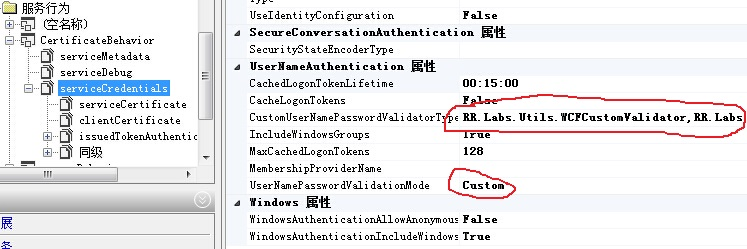
\includegraphics[scale=0.8]{CustomValidateServerConfig.jpg}
	\caption{自定义验证界面配置}
	\label{fig:CustomValidateServerConfig}
\end{figure}

\paragraph{WCF之MemberShip验证}

在数据库中创建一个用于WCF认证的账户,如下代码所示。

\begin{lstlisting}[language={[Sharp]C},caption=MemberShip创建用户]
public void CreateUser()
{
    if (Membership.FindUsersByName("jiangxiaoqiang").Count == 0)
    {
        Membership.CreateUser("jiangxiaoqiang", "jiangxiaoqiang", "jiangtingqiang@gmail.com");
    }
}
\end{lstlisting}

System.Web节点的配置。

\begin{lstlisting}
<system.web>
	<compilation debug="true" targetFramework="4.0" />
	<membership defaultProvider="SqlProvider">
	  <providers>
	    <clear />
	    <add name="SqlProvider"
	         type="System.Web.Security.SqlMembershipProvider"
	         connectionStringName="WCFCredential"
	         applicationName="demosite"
	         enablePasswordRetrieval="false"
	         enablePasswordReset="true"
	         requiresQuestionAndAnswer="false"
	         requiresUniqueEmail="true"      
	         passwordFormat="Hashed" />
	  </providers>
	</membership>
	<httpRuntime maxRequestLength="20000000" executionTimeout="600" requestValidationMode="2.0" />
</system.web>
\end{lstlisting}

\subsection{WCF RESTful Security}

在SOAP协议的WCF中,可以通过SOAPHeader(MessageHeader)来实现用户名密码的传输,
早在WebService时代我们就这么用过了。
在REST WCF中,我们可以利用 HttpHeader 来完成这一目标。
在每个服务契约里加上用户和密码的参数的设计肯定会成为你的噩梦。
首先在服务端的服务中加入如\ref{WCFCheckAuthorization}方法用于校验Header的信息:
如果Header中Authorization的字符串不是"123" 那么就将返回405 MethodNotAllowed 的错误。
这个字符串的内容可以自定义,服务端根据某种规则检查这个字符串。

\begin{lstlisting}[language={[Sharp]C},caption=WCF验证方法,label=WCFCheckAuthorization]
private bool CheckAuthorization()
{
    var ctx = WebOperationContext.Current;
    var auth = ctx.IncomingRequest.Headers[HttpRequestHeader.Authorization];
    if (string.IsNullOrEmpty(auth) || auth != "123")
    {
        ctx.OutgoingResponse.StatusCode = HttpStatusCode.MethodNotAllowed;
        return false;
    }
    return true;
} 
\end{lstlisting}

可以在服务提供的接口中调用此方法进行验证,
如代码\ref{WCFInvokeCheckAuthorization}所示。

\begin{lstlisting}[language={[Sharp]C},caption=WCF调用验证方法,label=WCFInvokeCheckAuthorization]
public string GetData(string a)
{
    if (!CheckAuthorization())
    {
        return "Access Failed!";
    }
    else
    {
        return "OK!You enter:" + a.ToString();
    }
}
\end{lstlisting}


当服务接口较多时,不可能每个方法都调用CheckAuthorization来进行验证,
以后的修改也会变得麻烦。
为了避免此问题,
采用自定义HTTP模块\footnote{\url{https://msdn.microsoft.com/zh-cn/library/ms227673\%28v=vs.100\%29.aspx}}
(Custom HTTP Module)来对每个提交的Request请求的合法性进行验证。
HTTP自定义模块通常具有以下用途:第一就是安全。
因为您可以检查传入的请求,
所以HTTP模块可以在调用请求页、XML Web services或处理程序之前执行自定义的身份验证或其他安全检查。
在以集成模式运行的Internet信息服务(IIS)7.0中,
可以将Forms身份验证扩展到应用程序中的所有内容类型。
在自定义模块的初始化方法中添加请求调用时触发的事件:

\begin{lstlisting}[language={[Sharp]C}]
public void Init(HttpApplication context)
{
    context.BeginRequest +=
    (new EventHandler(this.Application_BeginRequest));
}
\end{lstlisting}

调用验证方法:

\begin{lstlisting}[language={[Sharp]C}]
private void Application_BeginRequest(Object source, EventArgs e)
{
    HttpApplication application = source as HttpApplication;
    HttpContext context = application.Context;
    if (context != null)
    {
        CheckAuthorization(context);
    }           
}
\end{lstlisting}

验证不通过时手动向客户端抛出错误:

\begin{lstlisting}[language={[Sharp]C}]
private bool CheckAuthorization(HttpContext context)
{
    string auth = context.Request.Headers["Authorization"];            
    if (string.IsNullOrEmpty(auth) || auth != "123")
    { 
        throw new HttpException(404, "HTTP/1.1 404 Unauthorized");                              
    }
    return true;
}
\end{lstlisting}

HttpContext封装了ASP.NET要处理的单次请求的所有信息。
HttpContext的生存周期:从客户端用户点击并产生了一个向服务器发送请求开始
到服务器处理完请求并生成返回到客户端为止。
针对每个不同用户的请求,服务器都会创建一个新的HttpContext实例直到请求结束,服务器销毁这个实例。
HttpContext类,它对Request、Respose、Server等等都进行了封装,
并保证在整个请求周期内都可以随时随地的调用。
ASP.NET中它还提供了很多特殊的功能。
例如Cache、还有HttpContext.Item,
通过它你可以在HttpContext的生存周期内提前存储一些临时的数据,方便随时使用。

\subsubsection{采用SHA1签名认证}

客户端通过HttpWebRequest提交HTTP请求,
用HttpWebResponse接收请求,
在Request的Header中附加签名的Key-Value信息。
获取的签名字符串还可以通过MD5加密一次,
带签名的请求代码如\ref{code:SHA1SignatureRequest}所示。

\begin{lstlisting}[language={[Sharp]C},caption=客户端请求WCF接口,label={code:SHA1SignatureRequest}]
/// <summary>  
/// GET请求与获取结果(带签名)  
/// </summary>  
/// <param name="url">请求的WCF地址</param>
/// <param name="privateKey">生成签名的私钥</param>
/// <param name="postDataParam">请求参数集合</param>
public static string HttpGet(string url, string postDataParam,string privateKey)
{
    string postUrl = url + (postDataParam == "" ? "" : "?") + postDataParam;
    HttpWebRequest request = (HttpWebRequest)WebRequest.Create(postUrl);
    request.Method = "GET";
    request.ContentType = "text/html;charset=UTF-8";
    string signatureData = Encrypter.HashAndSignString(postUrl, privateKey);
    request.Headers.Add("Authorization", signatureData);
    HttpWebResponse response = (HttpWebResponse)request.GetResponse();
    Stream myResponseStream = response.GetResponseStream();
    StreamReader myStreamReader = new StreamReader(responseStream, Encoding.UTF8);
    string resultString = myStreamReader.ReadToEnd();
    myStreamReader.Close();
    myResponseStream.Close();
    return resultString;
}
\end{lstlisting}

url的地址形如\url{http://192.168.1.254:5590/WCFService/Custom/Service1.svc/web/GetData},
postDataParam形如id=18格式。服务端的验证方法如\ref{code:verifySignature}所示。
方法中将签名信息添加到请求头中,

\begin{lstlisting}[language={[Sharp]C},caption=服务端验证请求,label={code:verifySignature}]
/// <summary>
/// 验证签名
/// </summary>
/// <param name="context">HttpContext实例</param>
/// <returns>验证结果</returns>
private bool CheckAuthorization(HttpContext context)
{	
    string signatureData = context.Request.Headers["Authorization"];
    if (!string.IsNullOrEmpty(signatureData))
    {
        string publicKey = Developer.GetDeveloperPublicKeyByAppSecretKey("12");
        string originalText = context.Request.Url.OriginalString;
        bool sucess = SecurityUtil.VerifySigned(originalText, signatureData, publicKey);
        if (!sucess)
        {
            throw new HttpException(404, "HTTP/1.1 404 Unauthorized");
        }
    }
    else
    {
        //throw new HttpException(404, "HTTP/1.1 404 Unauthorized");
        //context.Response.End();
    }
    return true;
}
\end{lstlisting}

在浏览服务时,需要将代码throw new HttpException(404,"HTTP/1.1 404 Unauthorized")注释,
否则报\emph{未找到资源}错误。
或者采用context.Response.End()语句结束此次请求。
End方法使Web服务器停止处理脚本并返回当前结果。
文件中剩余的内容将不被处理。

\subsubsection{WCF REST HTTPS}

\subsection{WCF不使用svc文件}

无(.SVC)文件服务激活(File-Less Activation)是WCF 4.0的新特性。
在system.serviceModel配置节下添加如下配置。

\begin{lstlisting}
<serviceHostingEnvironment>
  <serviceActivations>
    <add relativeAddress="WCFService/Custom/RemoveSvcService.svc" service="RR.API.WCFService.Custom.RemoveSvcService"/>
  </serviceActivations>
</serviceHostingEnvironment>
\end{lstlisting}

service为带命名空间的类的名称。
service和factory对用着原来定义在.svc文件中<\%@ServiceHost>指令的Service和Factory属性,
而relativeAddress则表示服务相对服务寄宿的IIS站点的地址,该地址必须以.svc为后缀。

\subsection{WCF自定义路由映射}

WCF自定义路由映射是将形如:
\url{http://localhost/applicationname/Serivce.svc/Name}的地址映射为形如:
\url{http://localhost/applicationname/aa/Name}的地址。
首先在Global.asax中的Application\_Start事件中调用以下方法:

\begin{lstlisting}[language={[Sharp]C}]
public static void RegisterRoutes(RouteCollection routes)
{
    routes.EnableFriendlyUrls();
    WebServiceHostFactory factory = new WebServiceHostFactory();
    RouteTable.Routes.Add(new ServiceRoute("aa", factory, typeof(ConferenceService)));
}
\end{lstlisting}

Global.asax在程序第一次请求时访问,
且只访问一次。
使用EnableFriendlyUrls属性需要引用Microsoft.AspNet.FriendlyUrls.dll。
重定向成功后访问的页面如图\ref{fig:WCFRESTRedictUrl}所示。

\begin{figure}[htbp]
	\centering
	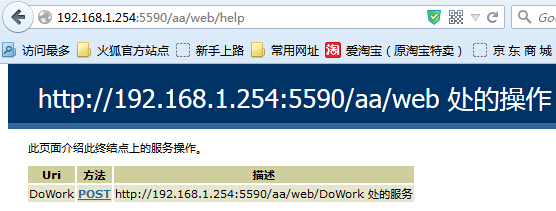
\includegraphics[scale=0.8]{WCFRESTRedictUrl.jpg}
	\caption{WCF Url路由}
	\label{fig:WCFRESTRedictUrl}
\end{figure}

原始的访问地址为:
\url{http://192.168.1.254:5590/WCFService/Custom/RemoveSvcService.svc/web/help},
经过Url路由后的访问地址为:
\url{http://192.168.1.254:5590/aa/web/help}。
配置文件中添加如下配置。

\begin{lstlisting}
<system.serviceModel>
  <serviceHostingEnvironment aspNetCompatibilityEnabled="true"/>
</system.serviceModel>
\end{lstlisting}

在添加路由之后无法访问初始页面,
使用路由重置的方式有点类似Web API, 
本身要出现元数据界面就是需要一个.svc,
现在的很像一个一般处理程序或Web API所以没有界面可以预览。

自定义路由的类上添加如下内容:

\begin{lstlisting}
[AspNetCompatibilityRequirements(RequirementsMode = AspNetCompatibilityRequirementsMode.Allowed)]
\end{lstlisting}

\subsection{WCF传递Cookie}

这是一个服务器与服务器的通讯,客户端(web应用)并不会自动发送cookie到wcf。
所以客户端还得做更多的工作核心在IClientMessageInspector这个接口,
他有BeforeSendRequest和AfterReceiveReply两个方法。
我们的目的是在beforeSendRequest时,
在请求中加入cookie信息,在AfterReciveReply方法中,
从响应中获取要设置的cookie,并真正设置到客户端。
首先使用的绑定,必须允许Cookie传播

\begin{lstlisting}
<wsHttpBinding>
	<binding name="CertificateBinding" 
	         messageEncoding="Mtom"
	         allowCookies="True">
	  <security>
	    <transport clientCredentialType="None" />
	    <message clientCredentialType="UserName" negotiateServiceCredential="false"/>
	  </security>          
	</binding>
</wsHttpBinding>
\end{lstlisting}

服务需要基于ASP.NET 的激活进行host。

\begin{lstlisting}
<!--运行服务以ASP.NET激活模式激活服务-->
<serviceHostingEnvironment aspNetCompatibilityEnabled ="true" multipleSiteBindingsEnabled="true" />
\end{lstlisting}

服务的实现,基于属性的声明允许以ASP.NET的方式访问

\begin{lstlisting}
[AspNetCompatibilityRequirements(RequirementsMode = AspNetCompatibilityRequirementsMode.Allowed)]
\end{lstlisting}

实现客户端的消息发送,响应拦截器。

\begin{lstlisting}[language={[Sharp]C}]
public class CookieMessageInspector : IClientMessageInspector
{
    public void AfterReceiveReply(ref Message reply, object correlationState)
    {
        return;
    }

    public object BeforeSendRequest(ref Message request, IClientChannel channel)
    {
        var cookie = "example";
        HttpRequestMessageProperty httpRequestMessage;
        object httpRequestMessageObject;
        if (request.Properties.TryGetValue(HttpRequestMessageProperty.Name, out httpRequestMessageObject))
        {
            httpRequestMessage = httpRequestMessageObject as HttpRequestMessageProperty;
            if (string.IsNullOrEmpty(httpRequestMessage.Headers["Cookie"]))
            {
                httpRequestMessage.Headers["Cookie"] = cookie;
            }
        }
        else
        {
            httpRequestMessage = new HttpRequestMessageProperty();
            httpRequestMessage.Headers.Add("Cookie", cookie);
            request.Properties.Add(HttpRequestMessageProperty.Name, httpRequestMessage);
        }
        return null;
    }
}
\end{lstlisting}

实现CookieBehavior。

\begin{lstlisting}[language={[Sharp]C}]
public class CookieBehavior : IEndpointBehavior
{
    public void AddBindingParameters(ServiceEndpoint endpoint, BindingParameterCollection bindingParameters)
    {
        return;
    }

    public void ApplyClientBehavior(ServiceEndpoint endpoint, ClientRuntime clientRuntime)
    {
        clientRuntime.MessageInspectors.Add(new CookieMessageInspector());
    }

    public void ApplyDispatchBehavior(ServiceEndpoint endpoint, EndpointDispatcher endpointDispatcher)
    {
        return;
    }

    public void Validate(ServiceEndpoint endpoint)
    {
        return;
    }
}
\end{lstlisting}

在服务器端接收Cookie。

\begin{lstlisting}[language={[Sharp]C}]
try
{
    if (HttpContext.Current != null)
    {
        foreach (string s in HttpContext.Current.Request.Cookies.AllKeys)
        {           
        }
    }
    else
    {
        logger.Info("Request is null!");
    }
}
catch (Exception e)
{
    logger.Error("aa", e);
}
\end{lstlisting}

回传Cookie时,需在服务端设置Cookie,
如下所示:

\begin{lstlisting}[language={[Sharp]C}]
HttpContext.Current.Response.Cookies.Add(new HttpCookie("test123", "123"));
\end{lstlisting}

设置后回传的参数里会有Set-Cookie,如图\ref{fig:HttpResponseSetCookie}所示。

\begin{figure}[htbp]
	\centering
	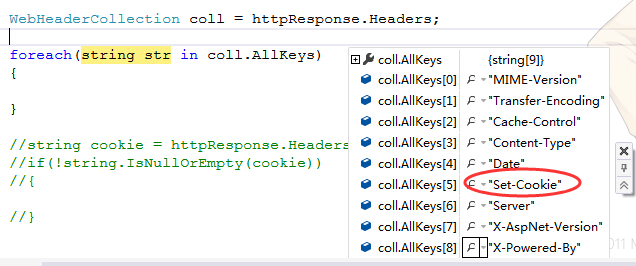
\includegraphics[scale=0.8]{HttpResponseSetCookie.jpg}
	\caption{回传参数中出现的Set-Cookie}
	\label{fig:HttpResponseSetCookie}
\end{figure}

Tips:在查看变量时,使变量锁定在当前页面也点击圆形的大头针图标。

\subsection{WCF REST传递Cookie}

在WCF里是可以使用session的。

在请求时添加如下语句:

\begin{lstlisting}[language={[Sharp]C}]
CookieContainer Cookie = new CookieContainer();
request.CookieContainer = Cookie;
\end{lstlisting}

\subsection{调取HTTPS类型的Web Service}

服务端的Web Service采用Java实现,在调取HTTPS类型的Web Service时跟调取普通的服务区别不大。
在传入HTTPS类型的URL时提示:提供的 URI 方案“https”无效,应为“http”。
只需要将配置文件的安全配置节修改为Transport即可,Transport代表采用HTTPS连接,
如下代码片段所示。

\begin{lstlisting}[language=XML]
<security mode="Transport" />
\end{lstlisting}

Transport seems to require HTTPS to encrypt credentials and throws an exception if there is no SSL. 
TransportCredentialsOnly will send the credentials in plain text and unencrypted and is recommended for testing ONLY!
所有的安全类型如表\ref{table:WebServiceSecurityChoice}所示:

\begin{table}\caption[Web Service Security Choice]{Security Choice}
	\label{table:WebServiceSecurityChoice}					
	\medskip
	\centering		
	\begin{tabular}{|c|p{10cm}|}
		\hline
		\multirow{1}{*}{Member Name}		
		& \multicolumn{1}{c|}{Description}\\			
		\cline{1-2}
		None &  The SOAP message is not secured during transfer. This is the default behavior.\\
		\hline
		Transport &  Security is provided using HTTPS. The service must be configured with SSL certificates. The SOAP message is protected as a whole using HTTPS. The service is authenticated by the client using the service’s SSL certificate. The client authentication is controlled through the ClientCredentialType.\\
		\hline	
	\end{tabular}
\end{table}

详细可参考:\url{https://msdn.microsoft.com/en-us/library/system.servicemodel.basichttpsecuritymode(v=vs.100).aspx}

\section{WCF异常处理}

在WCF开发阶段,如果想在客户端访问WCF时看到服务端详细的错误信息,
可增加配置。

\begin{lstlisting}[language=XML]
<serviceBehaviors>
  <behavior name="">
    <serviceMetadata httpGetEnabled="true" />
    <serviceDebug includeExceptionDetailInFaults="true" />
  </behavior>
</serviceBehaviors>
\end{lstlisting}

如上,在ServiceDebug节点中增加includeExceptionDetailInFaults, 赋值为true。
Enterprise Lib对WCF的支持中,Exception Block中还特地有针对WCF程序异常处理的解决方案,
而且满足以上说道的需求,即可记录异常,又可对异常信息进行封装。
更重要的是,自动处理运行时的异常信息,不需要挨个方法的去写Try catch。
秉承企业库的优秀传统,大部分工作还是通过配置就可以完成了,
非常好的解决方案。
Microsoft.Practices.EnterpriseLibrary.ExceptionHandling.dll

Microsoft.Practices.EnterpriseLibrary.ExceptionHandling.WCF.dll

Microsoft.Practices.EnterpriseLibrary.Common.dll

Microsoft.Practices.ObjectBuilder2.dll

安装完毕后Microsoft Enterprise Library的目录在
C:\textbackslash Program Files (x86)\textbackslash Microsoft Enterprise Library 5.0\textbackslash Bin下面。

\subsubsection{利用Attribute和IErrorHandler处理WCF全局异常}

实现IErrorHandler接口,实现他的两个方法。

\begin{lstlisting}[language={[Sharp]C},caption=实现IErrorHandler接口]
public class GlobalExceptionHandler : IErrorHandler
{
    /// <summary>
    /// 日志实例
    /// </summary>
    private readonly log4net.ILog logger = log4net.LogManager.GetLogger(MethodBase.GetCurrentMethod().DeclaringType);

    /// <summary>
    /// 
    /// </summary>
    /// <param name="error"></param>
    /// <returns>如果不应中止会话,则为true;否则为 false。默认值为 false。</returns>
    public bool HandleError(Exception error)
    {
        return true;
    }

    /// <summary>
    /// 
    /// </summary>
    /// <param name="error"></param>
    /// <param name="version"></param>
    /// <param name="fault"></param>
    public void ProvideFault(Exception error, MessageVersion version, ref Message fault)
    {
        logger.Error("WCF异常", error);
        /*定义抛给客户端的错误*/
        var clientException = new FaultException(string.Format("WCF接口出错 {0}", error.TargetSite.Name));
        MessageFault msgFault = clientException.CreateMessageFault();
        fault = Message.CreateMessage(version, msgFault, clientException.Action); 
    }
}
\end{lstlisting}

需要创建一个自定义的Service Behaviour Attribute,
让WCF知道当WCF任何异常发生的时候,通过这个自定义的Attribute来处理。
实现这个需要继承IServiceBehavior接口,并在此类的构造函数里,我们获取到错误类型。
一旦ApplyDispatchBehavior行为被调用时,
通过Activator.CreateInstance创建错误handler,
并把这个错误添加到每个channelDispatcher中。
channelDispatcher中文叫信道分发器,当我们的ServiceHost调用Open方法,
WCF就会创建我们的多个信道分发器(ChannelDispatcher),
每个ChannelDispatcher都会拥有一个信道监听器(ChannelListener),
ChannelListener就有一直在固定的端口监听,等到Message的到来,
调用AcceptChannel构建信道形成信道栈,开始对Message的处理。

\begin{lstlisting}[language={[Sharp]C},caption=实现IServiceBehavior接口]
public class GlobalExceptionHandlerBehaviourAttribute : Attribute, IServiceBehavior
{
    private readonly Type _errorHandlerType;

    public GlobalExceptionHandlerBehaviourAttribute(Type errorHandlerType)
    {
        _errorHandlerType = errorHandlerType;
    }

    public void AddBindingParameters(ServiceDescription serviceDescription, ServiceHostBase serviceHostBase, Collection<ServiceEndpoint> endpoints, BindingParameterCollection bindingParameters)
    {

    }

    public void ApplyDispatchBehavior(ServiceDescription serviceDescription, ServiceHostBase serviceHostBase)
    {
        var handler = (IErrorHandler)Activator.CreateInstance(_errorHandlerType);
        foreach (ChannelDispatcherBase dispatcherBase in serviceHostBase.ChannelDispatchers)
        {
            var channelDispatcher = dispatcherBase as ChannelDispatcher;
            if (channelDispatcher != null)
            {
                channelDispatcher.ErrorHandlers.Add(handler);
            }
        }
    }

    public void Validate(ServiceDescription serviceDescription, ServiceHostBase serviceHostBase)
    {

    }
}
\end{lstlisting}

最后在WCF的实现类上,加上GlobalExceptionHandlerBehaviour。

\begin{lstlisting}[language={[Sharp]C}]
[GlobalExceptionHandlerBehaviour(typeof(GlobalExceptionHandler))]
public class PublicBaseService : IPublicBaseService
{   
    public string DoWorkWithReturnValue(string a)
    {
        return a;
    }

    public void DoWork(string a)
    {
        int ia = 1;
        int b = 0;
        int c = ia / b;
    }
}
\end{lstlisting}

实现类中引发了一个除以0的异常,在全局中可以捕获到此异常,
如此在实现的代码中可省去try\{\}catch{}finally{}语句。

\subsection{常见问题}

\paragraph{安全包中没有可用的凭证}

将服务端的clientCredentialType改为UserName方式,如代码所示。

\begin{lstlisting}[language=XML]
<wsHttpBinding>
	<binding name="NewBinding0" messageEncoding="Mtom">
	  <security>
	    <transport clientCredentialType="None" />
	    <message clientCredentialType="UserName" negotiateServiceCredential="false"/>
	  </security>
	</binding>
</wsHttpBinding>
\end{lstlisting}

\paragraph{客户不能确定服务主体名称基于身份的目标地址http://myServerUrl”SspiNegotiation / Kerberos的目的。目标地址标识必须是UPN标识(如acmedomain/alice)或SPN身份(如主机/ bobs-machine)。}

禁用服务端的negotiateServiceCredential,
如代码所示\footnote{\url{http://www.cnblogs.com/artech/archive/2011/06/12/Authentication_043.html}}。

\begin{lstlisting}[language=XML]
<wsHttpBinding>
	<binding name="NewBinding0" messageEncoding="Mtom">
	  <security>
	    <transport clientCredentialType="None" />
	    <message clientCredentialType="UserName" negotiateServiceCredential="false"/>
	  </security>
	</binding>
</wsHttpBinding>
\end{lstlisting}

\paragraph{传入参数不能够和返回参数混合使用}

部署WCF时遇到如下错误:

\begin{quotation}
“The operation could not be loaded because it has a parameter or return type of type System.ServiceModel.Channels.Message or a type that has MessageContractAttribute and other parameters of different types. When using System.ServiceModel.Channels.Message or types with MessageContractAttribute, the method must not use any other type of parameters”.
\end{quotation}

这个错误说明WCF的传入参数不能够和返回参数混合使用,
比如传入的参数是基础类型,那么返回的参数也必须是基础类型,
传入的参数是对象,返回的参数也只能够是对象。

主要存在如下3中混合:

\begin{itemize}
\item{MixType1: Contract type and primitive types as operation parameters}
\item{MixType2: Contract type as a parameter and primitive type as return type}
\item{MixType3: Primitive type as a parameter and Contract type as return type}
\end{itemize}

\paragraph{远程服务器返回了意外响应: (400) Bad Request}

将远程服务调用的方法由GET改为POST,如代码所示。

\begin{lstlisting}[language={[Sharp]C},caption=改变调用方式]
[OperationContract]
[WebInvoke(Method="POST",UriTemplate = "GetAwardCount",
        ResponseFormat = WebMessageFormat.Json,
        BodyStyle = WebMessageBodyStyle.Wrapped)]
string GetAwardCount();
\end{lstlisting}

\paragraph{没有终结点在侦听可以接受消息的 http://192.168.1.254:5590/WCFService/Custom/PublicBaseService.svc。这通常是由于不正确的地址或者 SOAP 操作导致的。如果存在此情况,请参见 InnerException 以了解详细信息。}

出现此问题一般是服务端和客户端所选的绑定不一致导致。


\paragraph{此工厂上启用了手动寻址,因此发送的所有消息都必须进行预寻址}

添加behaviorConfiguration="webBehavior",如下代码所示。

\begin{lstlisting}[language=XML]
<behaviors>
  <endpointBehaviors>
    <behavior name="webBehavior">
      <webHttp/>
    </behavior>
  </endpointBehaviors>      
</behaviors>
<client>
  <endpoint name="employeeService"
            address="http://127.0.0.1:3721/employees" 
            behaviorConfiguration="webBehavior"
            binding="webHttpBinding" 
            contract="Artech.WcfServices.Service.Interface.IEmployees"/>
</client>
\end{lstlisting}


\paragraph{远程服务器返回了意外响应: (405) Method Not Allowed}

配置问题,一般通过客户端调用需要配置为basicHttpBinding。

\paragraph{无法使用以下搜索标准找到 X.509 证书}

\subsubsection{元数据包含无法解析的引用}

在服务端的service配置节下添加如下配置即可。

\begin{lstlisting}[language=XML]
<endpoint address="mex" binding="mexHttpBinding" contract="IMetadataExchange" />
\end{lstlisting}

\subsubsection{响应消息的内容类型 text/html; charset=utf-8 与绑定(multipart/related; type="application/xop+xml")的内容类型不匹配。如果使用自定义编码器,请确保正确实现 IsContentTypeSupported方法。响应的前 1024 个字节为:“<html>}

在浏览器中浏览地址试试能否成功浏览。

\subsubsection{接口页面无法找到}

WCF无法访问路由页面

\section{Web Service}

\subsection{SOAP调试}

SOAP的报文可以通过Fiddler抓取,
如果是采用SOAP UI做客户端,则可以先设置客户端的代理为Fiddler的代理,
然后可在请求时通过Fiddler抓取到请求的报文。
在Visual Studio中调用接口如果想看到SOAP请求,
可以设置Visual Studio的代理为Fiddler的代理地址即可。
设置Visual Studio的代理修改devenv.exe.config配置文件,
配置文件在:

\begin{lstlisting}
$VisualStudioInstallPath$\Program Files (x86)\Microsoft Visual Studio 12.0\Common7\IDE
\end{lstlisting}

在System.Net配置节下(与settings配置节平级)添加如下内容即可:

\begin{lstlisting}[language=XML]
<defaultProxy useDefaultCredentials="true" enabled="true">
	<proxy bypassonlocal="true" proxyaddress="http://127.0.0.1:8888/" />
</defaultProxy>
\end{lstlisting}

配置完毕后即可在Fiddler中看到SOAP请求,如图\ref{fig:FiddlerSOAPDebug}所示:

\begin{figure}[htbp]
	\centering
	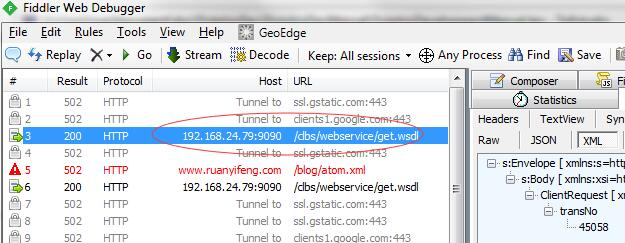
\includegraphics[scale=0.5]{FiddlerSOAPDebug.jpg}
	\caption{Fiddler调试Web Service}
	\label{fig:FiddlerSOAPDebug}
\end{figure}

\chapter{ASP.NET Web API(Apache License 2.0)}

\clearpage
\mbox{}         
\clearpage

ASP.NET Web API is a framework that makes it easy to build 
HTTP services that reach a broad range of clients, 
including browsers and mobile devices. 
ASP.NET Web API is an ideal platform for building RESTful applications on the .NET Framework.
在调用Web API时,传入的参数名称需要和服务器参数名称一致,
例如服务器的参数为function(string value),
那么调用是也必须在Url的参数集合中以value=1的形式,名称必须一致。
GlobalConfiguration.Configuration中GlobalConfiguration类在System.Web.Http.WebHost.dll中。

\section{Web Api帮助文档}

\subsection{Controller分类}

\paragraph{Step 2:继承DefaultHttpControllerSelector}The second part of the solution is to create an implementation of IHttpControllerSelector that actually uses the area name. 





\section{Web Api Area支持}

\section{Web Api路由}

请求路径以字符串”api”开头的时候将访问webAPI的函数
(注:至于为什么用MapHttpRoute而不是MapRoute;
为什么用routeTemplate而不是用url我们再以后的章节介绍)。
因为routeTemplate中有了{controller},
所以针对api的请求可以自动映射到指定的controller类。


\section{参数传递}


\subsection{Web Api Json传递}

http://blog.csdn.net/besley/article/details/23955147?utm\_source=tuicool\&utm\_medium=referral

\subsection{错误处理(Exception Handling in ASP.NET Web API)}

You can customize how Web API handles exceptions by writing an exception filter. 
An exception filter is executed when a controller method throws 
any unhandled exception that is not an HttpResponseException exception. 
The HttpResponseException type is a special case, 
because it is designed specifically for returning an HTTP response.
Exception filters implement the System.Web.Http.Filters.IExceptionFilter interface. 
The simplest way to write an exception filter is to derive from the System.Web.Http.Filters.ExceptionFilterAttribute class and override the OnException method.

\begin{lstlisting}[language={[Sharp]C},caption=Web API错误处理]
public class NotImplExceptionFilterAttribute : ExceptionFilterAttribute 
{
    public override void OnException(HttpActionExecutedContext context)
    {
        if (context.Exception is NotImplementedException)
        {
            context.Response = new HttpResponseMessage(HttpStatusCode.NotImplemented);
        }
    }
}
\end{lstlisting}

\subsection{消息处理(HTTP Message Handlers in ASP.NET Web API)}

A message handler is a class that receives an HTTP request 
and returns an HTTP response. Message handlers derive from the abstract HttpMessageHandler class.

Typically, a series of message handlers are chained together. 
The first handler receives an HTTP request, does some processing, 
and gives the request to the next handler. 
At some point, the response is created and goes back up the chain. 
This pattern is called a delegating handler\footnote{http://www.asp.net/web-api/overview/advanced/http-message-handlers}.

\subsection{Model绑定(Model Binding)}

Model binding is the process that maps data from request and supply to Action methods parameters. 
Model binding takes places after the authorization filters have executed and model is ready to bind. 
Model binder works with Value provides to get and map data. By default there 
are four value provides that MVC framework uses, Form Data, Route Data, 
Query string and posted Files. You can create your own custom value provider to choose data from, 
such as Cookie Value provider as custom value provider.

Model Binder is implemented from IModelBinder interface. 
By default, MVC provides a very powerful model binder but you can create your 
own custom model binder for your specific project needs. 
Model绑定不仅可以根据参数名(简单类型)从HTTPRouteData的value属性中提取同名的路由变量值
作为参数值。在ASP.NET MVC中,用户请求道服务器的数据将被包装为Model数据对象,
这个数据对象通常也被View用来提供显示的数据。在ASP.NET MVC中,
提供了非常灵活的Model绑定机制,通过IModelBinder借口,
定义了绑定Model数据的约定,并提供了一个接口的默认实现DefaultModelBinder。
在大多数情况下,仅仅通过DefaultModelBinder(System.Web.ModelBinding)就可以完成Model的绑定。
默认情况下,ASP.NET MVC使用DefaultModelBinder来绑定Model的数据。
在传递Action参数的时候,ASP.NET MVC按照如下顺序查找匹配的数据:

\begin{itemize}
\item{Form表单中的数据}
\item{RouteData中的数据}
\item{QueryString中的数据}
\end{itemize}
    
\section{Automated Documentation for REST APIs}

\subsection{安装Swagger-UI}

使用如下的命令安装Swagger-UI。

\begin{lstlisting}[language=Bash]
Install-Package Swashbuckle
\end{lstlisting}


\subsection{Swagger}

The goal of Swagger™ is to define a standard, 
language-agnostic interface to REST APIs which allows both humans 
and computers to discover and understand the capabilities 
of the service without access to source code, documentation, 
or through network traffic inspection. 
When properly defined via Swagger, 
a consumer can understand and interact with the remote service 
with a minimal amount of implementation logic. 
Similar to what interfaces have done for lower-level programming, 
Swagger removes the guesswork in calling the service.
Swagger-UI本身只提供在线测试功能,要集成它还需要告诉它本项目提供的各种服务和参数信息。

\begin{lstlisting}[language=HTML,caption=Swagger链接]
http://localhost:5509/swagger/ui/index
\end{lstlisting}

要让接口的内容显示,需要开启Web Api Tracing,
在WebApiConfig.cs文件的Rigester方法中添加如下语句。

\begin{lstlisting}[language={[Sharp]C},caption=开启Tracing]
config.EnableSystemDiagnosticsTracing();
\end{lstlisting}

需要注意的是EnableSystemDiagnosticsTracing为HttpConfiguration实例的扩展方法,
需要引用动态链接库System.Web.Http.Tracing,
另外需要注意的是Swagger对文件WebApiConfig.cs的名字大小写敏感。
测试页面虽然可以正常工作,但是接口说明和参数说明都是空着的,
显得不够友好,但这些实际是可以从代码的XML注释中读取出来的。
要实现这一效果,需要进行如下两步。首先,开放注释的XML文档的输出,
如图\ref{fig:WebApiOutputComment}所示。

\begin{figure}[htbp]
	\centering
	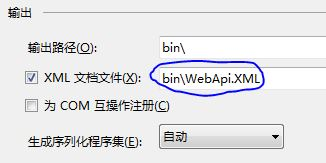
\includegraphics[scale=1]{WebApiOutputComment.jpg}
	\caption{输出注释}
	\label{fig:WebApiOutputComment}
\end{figure}

第二步就是将WebApi的注释(Comments)输出文档在SwaggerConfig.cs类中的Register方法进行指定,
如下代码片段所示。

\begin{lstlisting}[language={[Sharp]C},caption=Swagger指定注释文档的位置]
c.IncludeXmlComments(GetXmlCommentsPath());

private static string GetXmlCommentsPath()
{
    return System.String.Format(@"{0}\bin\WebApi.XML",System.AppDomain.CurrentDomain.BaseDirectory);
}
\end{lstlisting}

WebApi生成注释后的效果如图\ref{fig:WebApiCommentUI}所示,
所有的Api文档目前的粒度为Controller,Advert为Controller的名称,
GetAdvertise为Action的名称,往后项目复杂后可以根据模块分离出Area。

\begin{figure}[htbp]
	\centering
	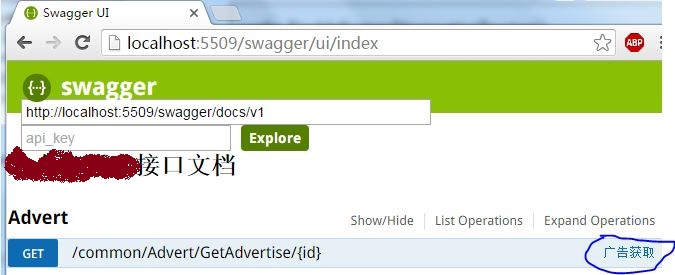
\includegraphics[scale=0.8]{WebApiCommentUI.jpg}
	\caption{注释的效果}
	\label{fig:WebApiCommentUI}
\end{figure}


\chapter{数据操作(Data Operate)}

\clearpage
\mbox{}         
\clearpage

\section{生成二维码(Generate QRCode)}

生成二维码需要引用ThoughtWorks.QRCode.dll文件,
使用里面的QRCodeEncoder类,初始化QRCodeEncodeMode、
QRCodeScale、QRCodeVersion、QRCodeErrorCorrect属性。
如下语句生成二维码:

\begin{lstlisting}[language={[Sharp]C},caption=生成二维码]
#region 创建二维码
/// <summary>
/// 
/// </summary>
/// <param name="data">二维码内容</param>
/// <returns></returns>
public string CreateQrCodeWithRelativePath(string data)
{
    var savePath = string.Empty;
    var qrCodeEncoder = new QRCodeEncoder
    {
        QRCodeEncodeMode = QRCodeEncoder.ENCODE_MODE.BYTE,
        QRCodeScale = 12,
        QRCodeVersion = 0,
        QRCodeErrorCorrect = QRCodeEncoder.ERROR_CORRECTION.M
    };
    try
    {
        var fileName = Guid.NewGuid() + ".png";
        var tempPath = Path.Combine(HttpRuntime.AppDomainAppPath, "qrcode\\");
        if (!Directory.Exists(tempPath))
        {
            Directory.CreateDirectory(tempPath);
        }
        savePath = tempPath + fileName;
        qrCodeEncoder.Encode(data, Encoding.UTF8).Save(savePath);
    }
    catch (Exception e)
    {
        PublicAttribute.Logger.Error("Generate QRCode encount an error", e);
    }
    return savePath;
}
#endregion
\end{lstlisting}

方法中获取Web程序当前运行的主目录的语句为:

\begin{lstlisting}
HttpContext.Current.Server.MapPath("/")
\end{lstlisting}

但是此种方法获取路径并不安全,
因为有时HttpContext.Current为null,
如定时器的回调、Cache的移除通知、APM模式下异步完成回调、
主动创建线程或者将任务交给线程池来执行时。
所以尽量避免使用MapPath,HttpRuntime.AppDomainAppPath才是更安全的选择。
此处获取的目录为:D:\textbackslash 项目\textbackslash zouwo\textbackslash RR.DataCommon\textbackslash bin\textbackslash Debug,
传入不同的参数获取不同的路径,具体如下:

\begin{lstlisting}
Server.MapPath("/")    //返回应用程序根目录所在的位置 如 C:\Inetpub\wwwroot\
Server.MapPath("~")  //表示当前应用级程序的目录,如果是根目录,就是根目录,如果是虚拟目录,就是虚拟目录所在的位置 如:C:\Inetpub\wwwroot\Example\
注:等效于Server.MapPath("~")。
Server.MapPath("./")   //返回当前目录绝对路径
Server.MapPath("../")   //返回上一级目录的绝对路径
\end{lstlisting}

推荐使用一种更加安全的方式,代码如下:

\begin{lstlisting}[language={[Sharp]C}]
string filePath=System.IO.Path.Combine(HttpRuntime.AppDomainAppPath,"\\qrcode\\a.png");
\end{lstlisting}

HttpRuntime下的除了WEB中可以使用外,
非WEB程序也可以使用。
而HttpContext则只能用在WEB中。
因此,在可能的情况下,我们尽可能使用HttpRuntime。

\begin{itemize}
\item{Path.Combine中如果其中一个参数为 null ,会抛出异常}
\item{如果指定的路径之一是零长度字符串,则该方法返回其他路径。两个都是零长度字符串,则返回的就是 string.Empty}
\item{如果path2包含绝对路径,则该方法返回path2}
\item{path2不能以\textbackslash 和/开头的字符串, 如果是这个字符串开头的,则返回path2}
\end{itemize}

\subsection{获取程序运行路径}

有时需要从磁盘上读取配置文件,
此时需要指定配置文件的相对路径,
在Windows Service中获取当前的程序运行路径并获得配置文件相对路径如下代码片段所示。

\begin{lstlisting}[language={[Sharp]C}]
var currentDirectory = AppDomain.CurrentDomain.BaseDirectory;
var configFilePath = currentDirectory + @"Config\quartz_jobs.xml";
\end{lstlisting}

\section{序列化(Serialization)与反序列化(Deserialization)}

从有赞系统\footnote{有赞,曾用名口袋通,旨在为商户提供强大的微店铺和完整的微电商解决方案。
是一个免费的微商城平台。有赞是一个以产品技术为主的团队,2012年开始一直专注于有赞这个产品,
所属公司为杭州起码科技有限公司。}
查询出的订单数据返回为Json\footnote{JavaScript Object Notaion:JavaScript对象标记}串,
Json串的简化版本如下代码片段所示:

\begin{lstlisting}
{
    "response": {
        "total_results": 33,
        "trades": [
            {
                "tid": "E231958349",
                "num": 1,                
                "buyer_type": 1,  
                "seller_flag": "5", 
                "orders": [
                    {
                        "oid": 14776,
                        "num_iid": 3424234,
                        "sku_id": 32221, 
                        "discount_fee": 0,
                        "payment": 200.02,
                        "buyer_messages": [
                            {
                                "title": "\u989c\u8272\u8981\u6c42",
                                "content": "\u7ea2\u8272\u7684\u6216\u8005\u9ec4\u8272\u7684"
                            },
                            {
                                "title": "\u989c\u8272\u8981\u6c42",
                                "content": "\u7ea2\u8272\u7684\u6216\u8005\u9ec4\u8272\u7684"
                            }
                        ],                       
                    }]
                    }]
               }
}
\end{lstlisting}

此处需要将返回的Json串转化为对应的有赞系统的Model,再将Model映射为本系统的Model持久化到数据库中。
根据Json串的结构,定义ResponseContainer、ResponseModel、TradeModel、OrderModel,每一个
Model分别对应Json串的response、trades、orders,在定义时需要注意每个属性的名称需要和Json串中的名称
完全一致。每个Model的定义如下代码片段所示:

\begin{lstlisting}[language={[Sharp]C}]
public class ResponseContainer
{
    public ResponseModel response { get; set; }        
}
\end{lstlisting}

\begin{lstlisting}[language={[Sharp]C}]
public class ResponseModel
{
    public int total_results { set; get; }
    public List<TradeModel> trades{ set; get;}        
}
\end{lstlisting}

如下代码片段是交易的Model:

\begin{lstlisting}[language={[Sharp]C}]
public class TradeModel
{
    #region Attribute 
    
    #region 订单
    private List<OrderModel> orders;

    public List<OrderModel> Orders
    {
        get { return orders; }
        set { orders = value; }
    }
    #endregion

    #endregion
}
\end{lstlisting}

如下代码片段是订单的Model:

\begin{lstlisting}[language={[Sharp]C}]
public class OrderModel
{
    #region Attribute    

    #region 价格
    private string price;

    public string Price
    {
        get { return price; }
        set { price = value; }
    }
    #endregion
}
\end{lstlisting}

将Json转换为Model的代码如下代码片段所示,通过调用Newtonsoft.Json.dll中的JsonConvert方法:

\begin{lstlisting}[language={[Sharp]C}]
#region Json反序列化为ResponseModelContainer
/// <summary>
/// Json反序列化为ResponseModelContainer
/// </summary>
/// <param name="json"></param>
/// <returns></returns>
public static ResponseContainer MapResponseJsonToContainer(string json)
{   
    ResponseContainer container = new ResponseContainer();
    try
    {
        container = JsonConvert.DeserializeObject<ResponseContainer>(json);
    }
    catch(Exception e)
    {
        logger.Error("Json转换过程中遇到错误",e);
    }
    return container;
}
#endregion
\end{lstlisting}

在Json与微信交互时,微信接收的Json的key只能小写(截止文章撰写时),
而在C\#中定义属性时采用驼峰命名法更合适,
所以在传入Json请求时需要统一将Json的key转化为小写\footnote{参考链接:http://stackoverflow.com/questions/6288660/net-ensuring-json-keys-are-lowercase\#}。


\begin{lstlisting}[language={[Sharp]C},caption=Json序列化时key转换为小写]
public class LowercaseJsonSerializer
{
    private static readonly JsonSerializerSettings Settings = new JsonSerializerSettings
    {
        ContractResolver = new LowercaseContractResolver()
    };

    public static string SerializeObject(object o)
    {
        return JsonConvert.SerializeObject(o, Formatting.Indented, Settings);
    }

    public class LowercaseContractResolver : DefaultContractResolver
    {
        protected override string ResolvePropertyName(string propertyName)
        {
            return propertyName.ToLower();
        }
    }
}
\end{lstlisting}


使用小写转换方法:

\begin{lstlisting}[language={[Sharp]C},caption=转换实例]
var json = LowercaseJsonSerializer.SerializeObject(new { Foo = "bar" });
// { "foo": "bar" }
\end{lstlisting}

\subsection{序列化(Serialization)字典值}

程序有时需要动态的字典类型(Key-Value)的配置项,
一般的序列化方法不支持字典(Dictionary)类型的序列化,
可使用DataContractSerializer进行序列化,
输出的XML文件需要是可读格式(Readable,不是所有的配置都是一行),
可以采用XmlWriterSettings进行设置。

\begin{lstlisting}[language={[Sharp]C},caption=将字典序列化为XML文件]
/// <summary>
/// 序列化辅助方法
/// </summary>
/// <typeparam name="T"></typeparam>
/// <param name="instance">需要序列化的对象</param>
/// <param name="fileName">保存的文件名(全路径)</param>
private static void Serialize<T>(T instance, string fileName)
{
    var serializer = new DataContractSerializer(typeof(T));
    /*输出为良好缩进的格式化的XML数据*/
    var xmlWriteSettings = new XmlWriterSettings { Indent = true };
    using (var writer = XmlWriter.Create(fileName, xmlWriteSettings))
    {
        serializer.WriteObject(writer, instance);
    }
}
\end{lstlisting}

\subsection{反序列化XML}

\subsection{XML增加内容}

SelectSingleNode方法总是返回为null,
原因就在于上面的xml文档中使用了命名空间,
当xml中定义了命名空间时,在查找节点的时候需要使用下面的方法。



\subsection{XML删除内容}

\subsection{序列化时添加字段}

\subsection{fastjson反序列化泛型}

使用fastjson反序列化泛型时用TypeReference传入泛型类型:

\begin{lstlisting}[language=Java]
ArrayList<ClientVehicleInfo> clientVehicleInfo = JSON.parseObject(subscribeVehicles, new TypeReference<ArrayList<ClientVehicleInfo>>(){});
\end{lstlisting}

\section{数据转换}

\subsection{将DataTable转为List}

在从数据库中获取数据库的时候,我们经常会返回一个DataTable类型,然后将其转换为List集合。
代码如下:

\begin{lstlisting}[language={[Sharp]C},caption=将DataTable转换为List]
#region 将DataTable转换为List
/// <summary>
/// 
/// </summary>
/// <typeparam name="T"></typeparam>
/// <param name="dt"></param>
/// <returns></returns>
public static List<T> ConvertDataTableToList<T>(DataTable dt) where T : class,new()
{
    var propertyList = new List<PropertyInfo>();
    Type type = typeof(T);
    Array.ForEach(
        type.GetProperties(),
        propertyInfo =>
        {
            if (dt.Columns.IndexOf(p.Name) != -1)
            {
                propertyList.Add(propertyInfo);
            }
        });
    var objectList = new List<T>();
    foreach (DataRow row in dt.Rows)
    {
        var singleObject = new T();
        propertyList.ForEach(
            propertyInfo =>
            {
                if (row[p.Name] != DBNull.Value)
                {
                    propertyInfo.SetValue(singleObject, row[propertyInfo.Name], null);
                }
            });
        objectList.Add(singleObject);
    }
    return objectList;
}
#endregion
\end{lstlisting}

此处在转换的过程中使用了泛型,使用泛型可以有如下方面的优势:

\begin{itemize}
\item{泛型可以使代码更加简洁、清晰}
\item{提升程序的性能}
\item{类型安全}
\end{itemize}

其中T代表任意类型(枚举除外),ConvertDataTableToList <T>,说明我们在调用这个方法的时候,
同时要赋予方法名一个类型值,这个类型要和它的返回值类型一致(泛型是类型安全的),
Where:用于限制T的条件,例如where T : class,new()表示T只能是一个类,
或者一个类型对象。此方法在转换的过程中,会出现类型之间转换失败的问题,
在设置值的时候将值转换成实际的类型。SetValue语句改为:

\begin{lstlisting}[language={[Sharp]C}]
propertyInfo.SetValue(objectT, Convert.ChangeType(row[propertyInfo.Name], propertyInfo.PropertyType), null);
\end{lstlisting}

ChangeType(Object, TypeCode)方法将Object更改为TypeCode参数指定的类型(如果可能),
ChangeType往往用在不知道当前类型应当是什么的情况下进行类型的转换,如有个泛型方法

\begin{lstlisting}[language={[Sharp]C}]
T GetObject<T>(string str)
\end{lstlisting}

要求从string类型转换为指定的T类型,此时只能

\begin{lstlisting}[language={[Sharp]C}]
return (T)Convert.ChangeType(str, typeof(T));
\end{lstlisting}

因为str显式转为T肯定是不行的,只能ChangeType。

\subsection{Double转换}

double.TryParse和double.Parse两者最大的区别是,
如果字符串格式不满足转换的要求,Parse方法将会引发一个异常;
TryParse方法则不会引发异常,它会返回false,同时将result置为0。
实际上,早期的FCL\footnote{Framework Class Library,即Framework类库。}
中并没有提供TryParse方法,那时只能调用Parse方法,
如果转换类型失败,则要将值设定为一个初始值,同时必须要捕获异常,代码如下所示:

\begin{lstlisting}[language={[Sharp]C}]
string str = string.Empty;  
double d;  
try  
{  
    d = double.Parse(str);  
}  
catch (Exception ex)  
{  
    d = 0;  
}
\end{lstlisting}

Convert.ToDouble调用此方法ToDouble(Char)始终引发InvalidCastException。

\subsection{List与string的转换}

在开发中经常会用List<string>来保存一组字符串,
比如下面这段代码:

\begin{lstlisting}[language={[Sharp]C}]
List<string> studentNames = new List<string>();

studentNames.Add("John");
studentNames.Add("Mary");
studentNames.Add("Rose");
\end{lstlisting}

可是有时候,我们要从中获取一个字符串,字符串的内容就是集合中的内容,但是要用逗号隔开,下面的办法可以实现:

\begin{lstlisting}[language={[Sharp]C}]
string.Join(", ", studentNames.ToArray());
\end{lstlisting}

输出John, Mary, Rose。

\subsection{获取集合的列}

\begin{lstlisting}[language={[Sharp]C}]
var questionIdCollectionList = from qids in questionnaire.QuetionnaireModel.QuestionModelList
                               select qids.ID;
string questionIdCollection = string.Join(",", questionIdCollectionList.ToArray());
\end{lstlisting}

\subsection{去除List中重复的对象}

\paragraph{List的Distinct扩展方法}要实现对象的相等比较,需要实现IEquatable<T>,
或单独写一个类实现IEqualityComparer<T>接口。

\begin{lstlisting}[language={[Sharp]C}]
public class WantGoPlaceCompare : IEqualityComparer<tour_wantToPlacesModel>
{
    public bool Equals(tour_wantToPlacesModel x, tour_wantToPlacesModel y)
    {
        return x.objId == y.objId;
    }

    public int GetHashCode(tour_wantToPlacesModel obj)
    {
        return obj.objId.GetHashCode();
    }
}
\end{lstlisting}

Distinct函数在比较时,先比较的HashCode值,
扩展函数Distinct在内部使用了一个Set<T>的类来帮助踢掉重复数据,
而这个内部类使用的是hash表\footnote{散列表(Hash table,也叫哈希表),
是根据关键码值(Key value)而直接进行访问的数据结构。
也就是说,它通过把关键码值映射到表中一个位置来访问记录,
以加快查找的速度。这个映射函数叫做散列函数,
存放记录的数组叫做散列表。}的方式存储数据,
所以会调用到我们自定义类的GetHashCode函数,
如果返回的hashcode值不等,它就不会再调用Equels方法进行比较了。
使用List的Distinct方法来剔除重复数据如下代码片段所示:

\begin{lstlisting}[language={[Sharp]C}]
//去除List重复对象
wantGoIds = wantGoIds.Distinct(new WantGoPlaceCompare()).ToList();
\end{lstlisting}

\subsection{List中的元素排序}

\paragraph{使用Linq进行排序}

如下的代码按照司机出发时间(Starttime)降序(descending)排列。

\begin{lstlisting}[language={[Sharp]C}]
var sortedDriverActionInfos = from items in driverActionInfos orderby items.Starttime descending select items;
\end{lstlisting}

\subsection{Unix时间戳格式转换}

经常发现很多地方使用一个时间戳\footnote{时间戳,又叫Unix Stamp. 
从1970年1月1日(UTC/GMT的午夜)开始所经过的秒数,不考虑闰秒。}表示时间。
比如:1370838759表示2013年6月10日 12:32:39。
而更多地方使用如2013-6-10 12:32:39格式的时间, 
代码\ref{code:DateTimeTimeStamp}实现两种格式之间的互相转换。

\begin{lstlisting}[language={[Sharp]C},caption=时间戳与DateTime转换,label={code:DateTimeTimeStamp}]
/// <summary>
/// 时间戳转为DateTime格式时间
/// </summary>
/// <param name="timeStamp">Unix格式时间戳</param>
/// <returns>DateTime格式时间</returns> 
private DateTime StampToDateTime(string timeStamp)
{
    DateTime dateTimeStart = TimeZone.CurrentTimeZone.ToLocalTime(new DateTime(1970, 1, 1));
    long totalSecondTime = long.Parse(timeStamp + "0000000");
    TimeSpan toNow = new TimeSpan(totalSecondTime);
    return dateTimeStart.Add(toNow);
}

/// <summary>
/// DateTime时间格式转换为Unix时间戳格式
/// </summary>
/// <param name="time">需要转换的DateTime时间</param>
/// <returns>Unix格式时间戳</returns> 
private long DateTimeToStamp(System.DateTime time)
{
    System.DateTime startTime = TimeZone.CurrentTimeZone.ToLocalTime(new System.DateTime(1970, 1, 1));
    return (long)(time - startTime).TotalSeconds;
}
\end{lstlisting}

\subsection{Linq操作}

\paragraph{Linq分页}

使用Linq分页,如下代码所示:

\begin{lstlisting}[language={[Sharp]C}]
#region Linq获取OrderModel集合
/// <summary>
/// 
/// </summary>
/// <param name="PageSize"></param>
/// <param name="CurPage"></param>
/// <param name="objs"></param>
/// <returns></returns>
private List<shop_orderModel> QueryByPage(int PageSize, int CurPage, List<shop_orderModel> objs)
{
    var query = from oneItem in objs select oneItem;
    return query.Take(PageSize * CurPage).Skip(PageSize * (CurPage - 1)).ToList();
}
#endregion
\end{lstlisting}

用以上方法确实能够得到分页的目的,但是当数据量大的情况下查询数据还是挺慢的,
因为我们是先把所有数据取出来后在进行分页的,而不是在数据库内就分页。
分页仅仅是把传入的对象按照要求进行排列,可以不用关心具体的分页对象,
此方法可以做如下改进:

\begin{lstlisting}[language={[Sharp]C}]
#region Linq获取sellerModel集合
/// <summary>
/// 
/// </summary>
/// <param name="PageSize"></param>
/// <param name="CurPage"></param>
/// <param name="objs"></param>
/// <returns></returns>
private List<T> QueryByPage<T>(int PageSize, int CurPage, List<T> objs)
{
    var query = from oneItem in objs select oneItem;
    return query.Take(PageSize * CurPage).Skip(PageSize * (CurPage - 1)).ToList();
}
\end{lstlisting}

采用泛型的方式做到分页时与传入的具体对象无关。
Linq中的take方法从序列开头传回指定的连接项目数目。
skip方法跳过序列中指定数量的元素,然后返回剩余的元素。

\paragraph{Linq非空判断}

有时在用Linq时,需要确定搜索的元素不为空,Linq如下:

\begin{lstlisting}[language={[Sharp]C}]
var resultRows = (from DataGridViewRow row in gridAlarmInfo.Rows.Cast<DataGridViewRow>().Where(row => row.Cells[12].Value != null)
				  where row.Cells[12].Value.ToString() == e.SerialNo.ToString()
				  select row).ToList();
\end{lstlisting}


\paragraph{Linq中的Any和All方法}

LINQ提供了两个布尔方法:Any()和All(),它们可以快速确定对于数据而言,
某个条件是true还是false。Any用于判断集合中是否有元素满足某一条件;不延迟。
(若条件为空,则集合只要不为空就返回True,否则为False)。
有2种形式,分别为简单形式和带条件形式,
下面是一个示例。

\begin{lstlisting}[language={[Sharp]C}]
var wantGoResult = from query in areadyGoneModel
where query.played == 1 && query.collectionStatus == 1
select query;
var isContains = wantGoResult.Any<tour_wantToPlacesModel>();
\end{lstlisting}

以上代码通过Linq语句根据条件查询一个集合areadyGoneModel,
使用any方法(返回bool)获得这个集合中是否有满足条件的元素(tour\_wantToPlacesModel)。
All方法则确定某一集合中是否所有的元素都满足某一特定条件。
以上语句可以简化为:

\begin{lstlisting}[language={[Sharp]C}]
var containsAreadyGone = areadyGoneModel.Any(areadyGome => areadyGome.played == 1 && areadyGome.collectionStatus == 1);
\end{lstlisting}

取出查询出来的实体直接用foreach循环结果即可。

\paragraph{Dictionary转换为List}

\begin{lstlisting}[language={[Sharp]C}]
var vechicleList = vechicleDicitonary.Select(vechicle => vechicle.Value).ToList();
\end{lstlisting}

\paragraph{Linq查询}

\begin{lstlisting}[language={[Sharp]C}]
from prod in db.Products
select prod.UnitPrice)
.Min()
\end{lstlisting}

\subsection{分页查询语句}

SQL Server可用如下语句进行分页查询,
此种分页语句适合SQL Server 2005及以上版本:

\begin{lstlisting}[language=SQL]
SELECT TOP 页大小 * 
FROM 
(
	SELECT ROW_NUMBER() OVER (ORDER BY id) AS RowNumber,* FROM table1
) A
WHERE RowNumber > 页大小*(页数-1)
\end{lstlisting}

页大小:每页的行数;页数:第几页。使用时,请把“页大小”和“页大小*(页数-1)”替换成数字。
一般情况下分页过程为:传入分页查询SQL,在数据库中获取到分页后的结果,
结果以DataTable的形式返回,再将DataTable转换为List集合展示在前台页面。
ROW\_NUMBER() OVER()为开窗函数,
在开窗函数出现之前存在着很多用SQL语句很难解决的问题,
很多都要通过复杂的相关子查询或者存储过程来完成。
为了解决这些问题,在2003年ISO SQL标准加入了开窗函数,
开窗函数的使用使得这些经典的难题可以被轻松的解决。
目前在MS SQL Server、Oracle、DB2 等主流数据库中都提供了对开窗函数的支持。
与聚合函数一样,开窗函数也是对行集组进行聚合计算,
但是它不像普通聚合函数那样每组只返回一个值,
开窗函数可以为每组返回多个值,因为开窗函数所执行聚合计算的行集组是窗口。
在ISO SQL规定了这样的函数为开窗函数,在 Oracle中则被称为分析函数,
而在DB2中则被称为OLAP函数。

开窗函数的调用格式为:

函数名(列) OVER(选项) 

OVER关键字表示把函数当成开窗函数而不是聚合函数。
SQL标准允许将所有聚合函数用做开窗函数,
使用OVER关键字来区分这两种用法。
开窗函数COUNT(*) OVER()对于查询结果的每一行都返回所有符合条件的行的条数。
OVER关键字后的括号中还经常添加选项用以改变进行聚合运算的窗口范围。
如果OVER关键字后的括号中的选项为空,则开窗函数会对结果集中的所有行进行聚合运算。    

\subsection{事务}

在代码中使用事务需要TransactionScope类,
TransactionScope存在于System.Transactions命名空间中,
它是从Framework 2.0开始引入的一个事务管理类,
它也是微软推荐使用的一个事务管理类。
在TransactionScope的构造函数中会自动创建了一个新的LTM(轻量级事务管理器),
并通过Transaction.Current隐式把它设置为环境事务。
在使用隐式事务时,事务完成前程序应该调用TransactionScope的Complete()方法,
把事务提交,最后利用Dispose()释放事务对象。若执行期间出现错误,事务将自动回滚。
在使用事务时操作系统需要启动MSDTC\footnote{msdtc.exe是微软分布式传输协调程序。
该进程调用系统Microsoft Personal Web Server和Microsoft SQL Server。
该服务用于管理多个服务器。msdtc:Microsoft Distributed Transaction Coordinator}服务,
可通过命令net start msdtc启动。使用如下代码所示。

\begin{lstlisting}[language={[Sharp]C}]
using (TransactionScope transactionScope = new TransactionScope())
{
    try
    {
        //事务操作          
        transactionScope.Complete();
    }
    catch (Exception e)
    {
        logger.Error("", e);        
    }
}
return success;
\end{lstlisting}

事务操作完毕调用Complete()方法进行提交,
遇到错误未执行Complete()时会自动回滚。

在抽取奖品的过程中,
为了防止多人同时抽奖(并发)时造成数据混乱,
保证抽取的奖品记录在高并发的情况下不被其他进程修改,
添加了行级锁,sql语句写法如下:

\begin{lstlisting}[language=SQL]
SELECT *
FROM   <TABLENAME>
WITH   (ROWLOCK,UPDLOCK,READPAST)
WHERE  CONDITION
\end{lstlisting}

ROWLOCK表示使用行级锁,而不使用粒度更粗的页级锁和表级锁。
UPDLOCK读取表时使用更新锁,而不使用共享锁,
并将锁一直保留到语句或事务的结束。
UPDLOCK的优点是允许您读取数据(不阻塞其它事务)并在以后更新数据,
同时确保自从上次读取数据后数据没有被更改。  
READPAST跳过锁定行。此选项导致事务跳过由其它事务锁定的行(这些行平常会显示在结果集内),
而不是阻塞该事务,使其等待其它事务释放在这些行上的锁。
如果第一次查询出行1,在第一次操作未结束时,
如有第二次查询会跳过第一次查询的行,
也即是第二次查询出的结果集中不包含第一次查询的行记录。
READPAST锁提示仅适用于运行在提交读隔离级别的事务,
并且只在行级锁之后读取。仅适用于SELECT语句。 

Granularity and isolation level and mode are orthogonal.

Granularity = what is locked = row, page, table (PAGLOCK, ROWLOCK, TABLOCK)

Isolation Level = lock duration, concurrency (HOLDLOCK, READCOMMITTED, REPEATABLEREAD, SERIALIZABLE)

Mode = sharing/exclusivity (UPDLOCK, XLOCK)

"combined" eg NOLOCK, TABLOCKX

\subsection{随机查询}

随机查询在SQL中的写法为:

\begin{lstlisting}[language=SQL]
select top 2  * 
from discount_seller
where isRecommand=1
order by newid()
\end{lstlisting}

此查询语句的作用为在标中符合isRecommand=1的结果集中随机选择2个结果。

\subsection{自定义异常(Custom Exception)}

在C\#中所有的异常类型都继承自System.Exception,
也就是说,System.Exception是所有异常类的基类. 
总起来说,其派生类分为两种:一是SystemException类,
所有的CLR提供的异常类型都是由SystemException派生。
ApplicationException类: 由用户程序引发,
用于派生自定义的异常类型,一般不直接进行实例化。
在程序中可以简单的进行异常的抛出,
在自定义异常类中统一进行异常的处理,
而不需要在类中进行日志的记录,
也算是封装变化点的实现方式之一(因为记录日志的工具可能发生变化,
那样就不需要到每一个类中去修改关于日志的代码,
在异常类中统一进行修改即可),
自定义异常如代码片段\ref{code:CustomException}所示。

\begin{lstlisting}[language={[Sharp]C},caption=自定义异常,label={code:CustomException}]
public class RestfulNullDataException : Exception
{
    public RestfulNullDataException()
    {

    }

    public RestfulNullDataException(string message)
    {
        PublicAttribute.Logger.Error(message);
    }

    public RestfulNullDataException(string message, Exception inner)
        : base(message, inner)
    {
        PublicAttribute.Logger.Error(message, inner);
    }
}
\end{lstlisting}


\subsection{根据经纬度计算距离}

根据地球之间2点的经纬度计算2点之间的距离,
Google提供的方法,公式为:

\begin{quotation}
\scalebox{1.2}{$S=2\arcsin\sqrt[]{\sin^2{(\frac{a}{2})}+\cos{(Lat1)}\times \cos(Lat2)
\times \sin^2{\frac{b}{2}}}\times 6378.1$}
\end{quotation}

公式中经纬度均用弧度表示,
角度到弧度的转化应该是很简单的了吧,
若不会,依然请参考这个这个经纬度算距离的工具;
Lat1 Lng1表示A点纬度和经度,
Lat2 Lng2表示B点纬度和经度(不要弄错顺序);
a = Lat1 – Lat2为两点纬度之差b = Lng1 -Lng2为两点经度之差;
6378.137为地球半径,单位为公里;
计算出来的结果单位为公里;
计算的代码如下所示:

\begin{lstlisting}[language={[Sharp]C}]
#region 根据经纬度计算2点之间距离
/// <summary>
/// 角度到弧度的转化
/// </summary>
/// <param name="d"></param>
/// <returns></returns>
private static double rad(double d)
{
    return d * Math.PI / 180.0;
}

/// <summary>
/// 
/// </summary>
/// <param name="lat1">A点纬度</param>
/// <param name="lng1">A点经度</param>
/// <param name="lat2">B点纬度</param>
/// <param name="lng2">B点经度</param>
/// <returns>返回距离(千米km)</returns>
public static double GetDistance(double lat1, double lng1, double lat2, double lng2)
{    
    double a = rad(lat1) - rad(lat2);
    double b = rad(lng1) - rad(lng2);
    double distance = 2 * Math.Asin(Math.Sqrt(Math.Pow(Math.Sin(a / 2), 2) +
     Math.Cos(radLat1) * Math.Cos(radLat2) * Math.Pow(Math.Sin(b / 2), 2)));
    distance = distance * EARTH_RADIUS;
    distance = Math.Round(distance * 10000) / 10000;
    return distance;
}
#endregion
\end{lstlisting}

其中地球半径常数为:

\begin{lstlisting}[language={[Sharp]C}]
/// <summary>
/// 地球半径(单位:km)
/// </summary>
private const double EARTH_RADIUS = 6378.137;
\end{lstlisting}

验证是否计算准确数据集。

\begin{lstlisting}{language=plaintext}
/*
 * 石桥铺地铁站坐标:106.484957,29.532313(精度,纬度)
 * 歇台子地铁站坐标:106.498388,29.535303(精度,纬度)
 * 距离:1.35km
 */
\end{lstlisting}

\subsection{为数组元素添加单引号}

在做SQL查询时,有时需要将字符串变量置于单引号中作为查询条件,
快速将字符串数组添加单引号如代码片段\ref{code:AddSingleQuotesForArray}所示。

\begin{lstlisting}[language={[Sharp]C},caption=为字符串数组添加单引号,label={code:AddSingleQuotesForArray}]
string condition = string.Empty;
int[] a = { 12, 13, 14, 15 };
condition = a.Aggregate(condition, (current, i) => current + ("'" + i+"',")).Trim(',');
this.Text = condition;
 
输出结果为:'12','13','14','15'
\end{lstlisting}

这里是将数组、集合中的元素拼接为带引号的字符串,
方便放入SQL的in操作符中,
这个语法可以做一些复杂的聚合运算,例如累计求和,累计求乘积。
它接受2个参数,一般第一个参数是称为累积数(默认情况下等于第一个值),
而第二个代表了下一个值。
第一次计算之后,计算的结果会替换掉第一个参数,继续参与下一次计算。

\subsection{获取foreach循环索引}

在C\#开发中往往使用foreach循环语句来代替for循环语句。
foreach比for更加简洁高效。
for语句直接就存在索引变量,
但在实际操作中,使用foreach有时需要用到索引。
最容易想到的解决方法是在foreach语句外面定义索引变量,
然后在foreach语句内自加,以此获取索引。例如:

\begin{lstlisting}[language={[Sharp]C},caption=foreach获取当前索引号,label={code:foreachGetIndex}]
int i = 0;
foreach(var item in arr)
{
     i++;
     item....
}
\end{lstlisting}


这样是实现了,但是简单地使用IndexOf函数就可以获取到索引值,
更加简洁,如代码片段\ref{code:foreachGetIndexUsingIndexOf}:

\begin{lstlisting}[language={[Sharp]C},caption=foreach获取当前索引号,label={code:foreachGetIndexUsingIndexOf}]
foreach(var item in arr)
{
     int index = arr.IndexOf(item); //index 为索引值
     item....
}
\end{lstlisting}

还可以使用Lambda表达式获取索引号,如代码片段\ref{code:foreachGetIndexUsingLambada}。

\begin{lstlisting}[language={[Sharp]C},caption=foreach获取当前索引号,label={code:foreachGetIndexUsingLambada}]
foreach (var roadLineModel in roadLineModels.Select((currentModel, currentIndex) => new { currentModel, currentIndex }))
{
    @(roadLineModel.currentIndex)//当前索引号
    @(roadLineModel.currentModel.lineId)//当前实体              
}
\end{lstlisting}


\subsection{byte操作}

不論是Socket or Serial都是要使用byte[]格式,所以學會轉byte[]是寫程式需要處理的第一步。
将byte[]转换为string:

\begin{lstlisting}[language={[Sharp]C}]
var str = System.Text.Encoding.Default.GetString(result);
\end{lstlisting}

将byte[]转换为十六进制(Hexadecimal)字符串:

\begin{lstlisting}[language={[Sharp]C}]
public static string ByteArrayToString(byte[] byteArr)
{
	string hex = BitConverter.ToString(byteArr);
	return hex.Replace("-","");
}
\end{lstlisting}

将十六进制字符转换为byte[],如下代码片段所示:

\begin{lstlisting}[language={[Sharp]C}]
public byte[] StringToByteArray(string hex) {
	return Enumerable.Range(0, hex.Length)
					 .Where(x => x % 2 == 0)
					 .Select(x => Convert.ToByte(hex.Substring(x, 2), 16))
					 .ToArray();
}
\end{lstlisting}

将整型int转换为byte[],也可以适用于将ushort类型转换为byte[],
阵列索引值越低,存放高位元组,這称为 Big Endian,
字串由左至右阅读,转换后,阵列索引值越低,存放低位元组,这称为Little Endian,
使用BitConverter转换默认情况下为Little Endian,
Little Endian和Big Endian只是排列分布顺序颠倒而已,就看Server吃什么样的顺序,
网络字节序:TCP/IP各层协议将字节序定义为Big-Endian,
因此TCP/IP协议中使用的字节序通常称之为网络字节序。
我们可以透过Array.Reverse方法來顛倒阵列的顺序,如下代码片段所示:

\begin{lstlisting}[language={[Sharp]C}]
byte[] bytes = BitConverter.GetBytes(i);
//如果是小端,转化为大端,因为TCP/IP定义的是大端(Big-Endian)
if(BitConverter.IsLittleEndian) Array.Reverse(hex)
\end{lstlisting}

互联网使用的网络字节顺序采用大端模式进行编址,而主机字节顺序根据处理器的不同而不同,
如PowerPC处理器使用大端模式,而Pentuim处理器使用小端模式。
The order of bytes in the array returned by the GetBytes method depends on whether the computer architecture is little-endian or big-endian.
将12位手机号转换为6字节数组BCD码:

\begin{lstlisting}[language={[Sharp]C}]
public byte[] ConvertToBcd6(string mobileNo)
{
	var mobileArray = new byte[6];
	if (mobileNo.Length != 12) return mobileArray;
	for (var i = 0; i < 6; i++)
	{
		mobileArray[i] = Convert.ToByte(mobileNo.Substring(i * 2, 2), 16);
	}
	return mobileArray;
}  
\end{lstlisting}

\paragraph{Decimal转换为BCD}

较通用的将Decimal转换为BCD.

\begin{lstlisting}[language={[Sharp]C}]
private IEnumerable<Byte> DecimalToBcd(Decimal value)
{
	Byte currentByte = 0;
	Boolean odd = true;
	while (value > 0)
	{
		if (odd)
			currentByte = 0;
		Decimal rest = value % 10;
		value = (value - rest) / 10;
		currentByte |= (Byte)(odd ? (Byte)rest : (Byte)((Byte)rest << 4));
		if (!odd)
			yield return currentByte;
		odd = !odd;
	}
	if (!odd)
		yield return currentByte;
}  
\end{lstlisting}


\subsection{获取字符串中的数字}

获取字符串中的数字方法如下:

\begin{lstlisting}[language={[Sharp]C}]
public string GetNumberFromString(string mixedString)
{
	var resultNumber = string.Empty;
	for (var i = 0; i < mixedString.Length; i++)
	{
		if (char.IsNumber(mixedString, i))
		{
			resultNumber += mixedString.Substring(i, 1);
		}
		else
		{
			if (mixedString.Substring(i, 1) == ",")
			{
				resultNumber += mixedString.Substring(i, 1);
			}
		}
	}
	return resultNumber;
}
\end{lstlisting}


\section{Windows服务(Windows Service)}

实现从有赞系统定时将订单数据导入本地数据库,导入的同时,对购买商品的用户
发送短信通知,具体的整体流程如图\ref{YZLogic}所示:

\subsection{Demo}

服务需要继承自ServiceBase类,服务的应用程序入口点如下代码片段所示:

\begin{lstlisting}[language={[Sharp]C}]
static void Main()
{
    ServiceBase[] ServicesToRun;
    ServicesToRun = new ServiceBase[] 
	{ 
		new OrderImportService()             
	};

    ServiceBase.Run(ServicesToRun);
}
\end{lstlisting}

其中OrderImportService为实现服务的类。

\subsection{调试服务}

可以通过如下命令操作Windows服务。

\begin{lstlisting}[language=Bash]
----安装Windows服务-----
C:\Windows\Microsoft.NET\Framework64\v4.0.30319>InstallUtil.exe -i D:\项目\zouwo\RRInterop\bin\Debug\RRInterop.exe

----卸载Windows服务-----
C:\Windows\Microsoft.NET\Framework64\v4.0.30319>InstallUtil.exe -u D:\项目\zouwo\RRInterop\bin\Debug\RRInterop.exe

----启动Windows服务-----
sc start OrderImportService

----停止Windows服务-----
sc stop OrderImportService
\end{lstlisting}

其中利用了InstallUtil工具。该工具的路径一般为:C:/Windows/Microsoft.NET/,
命令参数i即是install的缩写,u即是uninstall的缩写。sc为Service Controller
的缩写。与net.exe实用程序相比,sc.exe实用程序的功能更强大,可以检查服务的实际
状态,或者配置、删除以及添加服务。

\subsection{修改配置文件}

修改配置文件的方法为:

\begin{lstlisting}[language={[Sharp]C}]
#region change configuration file
/// <summary>
/// change configuration file
/// </summary>
/// <param name="createdTime"></param>
public void ChangeConfiguration(string createdTime)
{
	var exePath = System.AppDomain.CurrentDomain.BaseDirectory + @"\RRInterop.exe";     
    var appDomainConfigFile = AppDomain.CurrentDomain.SetupInformation.ConfigurationFile;
    var config = ConfigurationManager.OpenExeConfiguration(exePath);
    var appSettings = (AppSettingsSection)config.GetSection("appSettings");
    appSettings.Settings.Remove("queryTime");
    appSettings.Settings.Add("queryTime", createdTime);
    config.Save();
    ConfigurationManager.RefreshSection("configuration");
}
#endregion
\end{lstlisting}

保存后总是出现一个新文件App.config.config,
StackOverFlow上的解释\footnote{详细信息请参考链接:\url{http://stackoverflow.com/questions/30836963/
why-the-program-generate-a-new-configuration-file}}是:

\begin{quote}
This is because OpenExeConfiguration takes the exe name as input and automatically 
looks for a config file name exe.config (This is the default format).
\end{quote}

是因为修改配置文件时程序寻找的默认文件名格式为exe.config进行修改,这里要修改配置文件实际需要修改
命名格式为\textbf{程序名称+exe.config}
文件,且保存时自动添加config后缀,所以exePath写入程序名称即可。在获取程序运行路径exePath时,
应调用方法System.AppDomain.CurrentDomain.BaseDirectory。调用System.Environment.CurrentDirectory
\footnote{Gets or sets the fully qualified path of the current working directory.}
时获取的是路径C:\textbackslash System\textbackslash Windows32。

\subsection{读取配置文件}

读取配置文件时出现错误:未将对象引用设置到对象的实例。
可以通过如下语句查看当前配置文件所在路径:

\begin{lstlisting}[language={[Sharp]C}]
AppDomain domain = AppDomain.CurrentDomain;
string configFilePath = domain.SetupInformation.ConfigurationFile;
\end{lstlisting}

此处使用单元测试工具NUnit,
启动项目为NUnit的界面,
所使用的配置文件并不是bin目录下的配置文件。
配置文件的输出的路径为D:/项目zouwo/RRInterop/bin/Debug/Project1.config。
可知是Project1.config配置文件中没有连接串导致的此问题。
另在CS类型项目运行中配置文件信息默认从启动程序exe的配置文件中获取,
例如RRMall.WxPrint.Dal的配置信息从RRMall.WxPrint.exe.config中读取。

\section{字符串格式化(Format)}

\begin{lstlisting}[language={[Sharp]C}]
//250,000.00,默认保留2位小数,如果为{0:N1},则默认保留1位小数,N为Number的缩写
string result=string.Format("{0:N}", 250000);
\end{lstlisting}

\section{参数验证}

\subsection{代码契约(Code Contract)}

Microsoft 在 .NET 4.0 中正式引入契约式编程库。
契约式编程是一种相当不错的编程思想,
它不但可以使开发人员的思维更清晰,而且对于提高程序性能很有帮助。
值得一提的是,它对于并行程序设计也有莫大的益处。 

Contract的基本使用包括Requires和Ensures,
Requires在方法开始时检查初始条件是否满足,
通常用来做参数验证。Ensures方法用来在方法结束时检查执行结果是否符合预期,
比如可以放在Property set方法的末尾检查Property是否被正确设置。 
插件里的ccrewrite工具会将Contract方法编译成有效的检查代码分别注入函数体的首尾。
所以即使你把Contract.Ensures检查放在函数开头部分(这也是推荐做法),
编译之后这部分逻辑依然会出现在函数末尾,检查函数结束条件是否满足。

需要注意的是,如果想要在Debug和Release Build都使用运行时验证功能,
则需要在项目设置为Debug和Release编译时,分别设置打开Runtime check。

Contract有一个很酷的feature,就是可以在接口里定义一些检查,
要求所有的实现都满足这些检查条,这样就不用在接口的每个实现里分别定义相同的检查逻辑了,
非常的优雅,也符合Declaration Programming的初衷,如下代码所示。

\begin{lstlisting}[language={[Sharp]C}]
public void Invoke(string input)
{
    Contract.Ensures(!string.IsNullOrEmpty(input));
}
\end{lstlisting}

此处明确调用此方法的前置条件是参数input不能为空,
如果传入了非法的参数,
则会引发System.Diagnostics.Contracts.\_\_ContractsRuntime.ContractException类型的异常,
程序可以在合适的地点处理异常。

\subsection{验证小时分钟}

\begin{lstlisting}[language={[Sharp]C}]
#region 验证(小时-分钟时间格式)
/// <summary>
/// 
/// </summary>
/// <param name="shutdownTime"></param>
/// <returns></returns>
[TestCase("19:23", Result = true)]
[TestCase("09:00", Result = true)]
[TestCase("25:55", Result = false)]
[TestCase("00:00", Result = true)]
[TestCase("03:77", Result = false)]
[TestCase("", Result = false)]
public static bool IsValideShutdownTimeFormat(string shutdownTime)
{
    return Regex.IsMatch(shutdownTime, @"^(([0-1]\d)|(2[0-4])):[0-5]\d$");
}
#endregion
\end{lstlisting}

验证采用了正则表达式(Regular Expression),
\^ ~匹配开头,\$匹配结尾,[0-1]\textbackslash d匹配0到19之间的数字,
2[0-4]匹配20到23之间的数字。[0-5]\textbackslash d匹配0到59之间的数字。

\subsection{生成GUID}

注意:这里的D,N,B,P是不区分大小写的,如果传入空字符串,则使用的默认的D类型,其它情况都会报异常。

\begin{lstlisting}[language={[Sharp]C}]
var guid = Guid.NewGuid();

//10244798-9a34-4245-b1ef-9143f9b1e68a
Console.WriteLine(guid.ToString("D"));//D:hyphens,连字符,连(字)号

//102447989a344245b1ef9143f9b1e68a
Console.WriteLine(guid.ToString("N"));//N:digits,数字( digit的名词复数 ) 手指,足趾

//\{10244798-9a34-4245-b1ef-9143f9b1e68a\}
Console.WriteLine(guid.ToString("B"));//B:brace

//(10244798-9a34-4245-b1ef-9143f9b1e68a)
Console.WriteLine(guid.ToString("P"));//P:parentheses
\end{lstlisting}

\section{代码生成(Code Generate)}

\subsection{CSharpCodeProvider}

\begin{lstlisting}[language={[Sharp]C},caption=CSharpCodeProvider代码自动生成]
/// <summary>
/// 编译源代码
/// </summary>
/// <param name="sourceCodeContent"></param>
/// <param name="outAssemblyPath">DLL输出目录</param>
/// <param name="referencedAssemblies">编译时需引用的程序集</param>
/// <returns></returns>
public static bool CompileUtil(string sourceCodeContent, string outAssemblyPath, IEnumerable<string> referencedAssemblies)
{
    var compileSuccess = true;
    var compileInfo = string.Empty;
    var csharpCodePrivoder = new CSharpCodeProvider();
    var codeCompiler = csharpCodePrivoder.CreateCompiler();
    var compilerParameters = new CompilerParameters();
    foreach (var singleReference in referencedAssemblies)
    {
        //添加引用
        compilerParameters.ReferencedAssemblies.Add(singleReference);
    }
    compilerParameters.GenerateExecutable = false;
    compilerParameters.GenerateInMemory = false;
    compilerParameters.OutputAssembly = outAssemblyPath;
    var compilerResult = codeCompiler.CompileAssemblyFromSource(compilerParameters, sourceCodeContent);
    if (compilerResult.Errors.HasErrors)
    {
        foreach (CompilerError compilerError in compilerResult.Errors)
        {
            compileInfo += compilerError.ErrorText;
        }
        compileSuccess = false;
        LogHelper.Logger.Error("Compile error:" + compileInfo);
    }
    return compileSuccess;
}
\end{lstlisting}

\subsection{CodeDOMProvider}

\section{配置}

\subsection{ini}

INI文件格式是某些平台或软件上的配置文件的非正式标准,以节(section)和键(key)构成,
常用于微软Windows操作系统中。这种配置文件的文件扩展名多为INI,故名。
INI是英文“初始化”(initialization)的缩写。正如该术语所表示的,
INI文件被用来对操作系统或特定程序初始化或进行参数设置。

\subsection{自动注册COM组件}

\begin{lstlisting}[language={[Sharp]C}]
#region 是否已注册控件
/// <summary>
/// 
/// </summary>
/// <param name="classId"></param>
/// <returns></returns>
public static void IsDllRegisteredSuccess(string[] classId)
{
	foreach (var currentClassId in classId)
	{
		var registerKey = Registry.ClassesRoot.OpenSubKey("CLSID\\" + currentClassId);
		if (registerKey != null) continue;
		var i = DllRegisterServer();
		if (i < 0)
		{
			Log.Logger.Error("Control registered failed");
		}
		else
		{
			Log.Logger.Info("Control registered suceess");
		}
	}
}
#endregion
\end{lstlisting}

\section{集合操作}

\subsection{HashMap value to list}

What is the best way to convert a Map<key,value> to a List<value>:

\begin{lstlisting}[language=Java]
List<Value> list = new ArrayList<Value>(map.values());
\end{lstlisting}


\chapter{Web}

Web应用这些年来变得越来越强大,但相比于桌面应用能够完全访问计算机硬件,Web应用还有一些差距。

1999 HTML

2000 CGI

2001 asp

2002 xhtml

2003 flash

2004 ajax

2005 php perl java

2006 now-RIA

\clearpage
\mbox{}         
\clearpage

\subsection{URL规范}

URL规范化(url normalization)其实就是一个标准化URL的过程,
其实也就是将一个URL转化为一个符合规范的等价URL(如\url{http://www.cnblogs.com/shuchao}转化为\url{http://www.cnblogs.com/shuchao/}),
这样程序可以确定这两个URL是等价的。
URL规范化用于搜索引擎可以减少对页面的重复索引,
同时也可以减少爬虫的重复抓取。
浏览器端识别用户是否访问过一个URL也需要使用URL规范化。
Url的组成为:

\begin{lstlisting}
protocol://hostname[:port]/path/[;parameters][?query-string]\#fragment\\
协议://主机名[:端口]/ 路径/[:参数] [?查询]\#Fragment
\end{lstlisting}

\begin{itemize}
\item{protocol(协议)表示访问资源和服务的协议。例如http,ftp,mailto和file等。}
\item{hostname(主机名)表示资源所在主机的完全限定域名,例如www.schoolfree.com.cn。}
\item{port(端口)表示协议使用的TCP端口号,
具体的端口号是可选的,省略端口号时前面的冒号也要省略,
即表示采用"最著名的端口"。HTTP协议的常用端口为80。
一般的web服务器一个ip地址的80端口只能正确对应一个网站,
处理一个域名的访问请求。
而web服务器在不使用多个ip地址和端口的情况下,
如果需要支持多个相对独立的网站就需要一种
机制来分辨同一个ip地址上的不同网站的请求,
这就出现了主机头绑定的方法。
在IIS中,每个web站点都具有唯一的、由三个部分组成的标识,
用来接收和响应请求:

(1) ip地址;

(2)端口号;

(3)主机头名。}
\item{path(路径)表示资源的目录/文件路径名。}
\item{query-string表示发送给http服务器的数据。}
\item{search查找元素表示URL中传递的查询字符串。
查询字符串是通过QUERY\_STRING环境变量传递给ASP程序的参数。}
\item{hash散列符元素表示指定的文件偏移量,
包括散列符(\#)加上该文件偏移量相关的位置点名。}
\end{itemize}

\subsection{Uri}

URI、URL、URN三者的关系如图\ref{fig:RelationshipOfUriUrlUrn}所示。

\begin{figure}[htbp]
	\centering
	
\includegraphics[scale=0.5]{RelationshipOfUriUrlUrn.png}
	\caption{URI、URL、URN关系图}
	\label{fig:RelationshipOfUriUrlUrn}
\end{figure}

URL:(Uniform/Universal Resource Locator 的缩写,统一资源定位符)。

URI:(Uniform Resource Identifier 的缩写,统一资源标识符)。

关系:

URI 属于 URL 更低层次的抽象,一种字符串文本标准。
就是说,URI属于父类,而URL属于URI的子类。URL是URI的一个子集。
二者的区别在于,URI 表示请求服务器的路径,定义这么一个资源。
而 URL 同时说明要如何访问这个资源(http://)。

\subsection{CommonJS}

CommonJS是一种规范,NodeJS是这种规范的实现。
CommonJS是一个不断发展的规范,
CommonJS有很多实现,其中不乏很多大名鼎鼎的项目,
比如说:Apache的CouchDB和node.js等。
但这些项目大部分只实现了CommonJS的部分规范。

\section{通信}

\subsection{端口}

\paragraph{22} SSH为Secure Shell的缩写,由IETF的网络工作小组(Network Working Group)所制定;
SSH为建立在应用层和传输层基础上的安全协议。SSH是目前较可靠,专为远程登录会话和其他网络服务提供安全性的协议。
利用SSH协议可以有效防止远程管理过程中的信息泄露问题。SSH最初是UNIX系统上的一个程序,
后来又迅速扩展到其他操作平台。SSH在正确使用时可弥补网络中的漏洞。SSH客户端适用于多种平台。
几乎所有UNIX平台—包括HP-UX、Linux、AIX、Solaris、Digital UNIX、Irix,以及其他平台,都可运行SSH。

\subsection{Internet Information Service}

IIS运行时使用的3份配置文件如下:

\begin{lstlisting}
应用程序配置文件: E:\OneDrive\Source Code\Renrenmall\Tour\trunk\RR.Web.CCN.Tour\web.config
主机配置文件: C:\Windows\Microsoft.NET\Framework64\v4.0.30319\aspnet.config
C:\Windows\Microsoft.NET\Framework64\v4.0.30319\config\machine.config 的计算机配置文件。
\end{lstlisting}

在IIS 5.x中,存在如下两个方面的问题:
其一是ISAPI(Internet Server Application Programming Interface)动态链接库被加载到InetInfo.exe进程中,
它和工作进程(aspnet.exe)之间是一种典型的跨进程通信方式,
虽然采用命名管道,
但是仍然会带来性能的瓶颈.
为了解决这个问题,IIS 6.0将ISAPI动态链接库直接加载到工作进程(aspnet.exe)中.
其二是所有的ASP.NET应用运行在相同的进程(aspnet\_wp.exe)的不同程序域中,
基于应用程序域的隔离不能从根本上解决一个应用程序对另一个应用程序的影响,
更多时候需要不同Web运行在不同的进程中。
为了解决这个问题,在IIS 6.0中引入了应用程序池(Application Pool)的机制。
可以为一个或者多个应用创建一个应用程序池,
每一个应用程序池对应一个独立的工作进程(w3wp.exe),
所以运行在不同应用程序池中的Web应用提供基于进程级别的隔离机制\cite{蒋金楠MVC框架揭秘},
这也解释了为什么有时Windows进程中会同时运行多个w2wp.exe。
原则上,我们可以通过IIS访问置于虚拟目录下的所有Resource,
这部仅仅包含一些静态资源文件,比如图片、纯Html文件、CSS、JS等等,
也包含一些需要动态执行的文件,比如aspx,asmx等等,
我们还可以将Remoting和WCF Service Host到IIS下。
对于这些静态的文件,IIS直接提取对应的文件将其作为Http Response返回给Client,
但是对于这些需要进一步处理的动态执行的文件,
IIS必须将Request进一步传递给对应的处理程序,
待处理程序执行完毕获得最终的Http Response通过IIS返回给Client。
对于IIS来说,这些处理程序通过ISAPI Extension来体现。
对于基于ASP.NET的Resource,其对应的ISAPI Extension为ASP.NET ISAPI,
通过一个aspnet\_isapi.dll承载。
IIS的Metadata database维护着一个称为ISAPI Extension Mapping的数据表,
负责将不同类型的Resource影射到对应的ISAPI Extension。
常见映射关系如表\ref{table:IISApplicationMappings}所示。

\begin{table}\caption[Caption for LOF]{IIS Application Mappings for aspnet\_isapi.dll}
\label{table:IISApplicationMappings}					
	\medskip
	\centering		
	\begin{tabular}{|c|l|}
		\hline
		\multirow{1}{*}{Extension}		
		& \multicolumn{1}{c|}{Resource Type}\\			
		\cline{1-2}
		 .asax &  ASP.NET application files. Usually global.asax.\\
		\hline
		 .ascx & ASP.NET user control files.\\
		\hline
		 .ashx & HTTP handlers, the managed counterpart of ISAPI extensions.\\
		\hline
		 .asmx & ASP.NET web services.\\
		\hline
		 .aspx & ASP.NET web pages.\\
		\hline
		 .axd & ASP.NET internal HTTP handlers.\\
		 \hline
	\end{tabular}
\end{table}

\subsubsection{IIS与操作系统} 

IIS5.1集成于Windows XP操作系统中。

IIS6.0 集成于Windows Server 2003操作系统中。

IIS7.0 集成于 Windows Vista 和 Windows Server 2008操作系统中。

IIS7.5集成于Windows 7和Windows Server 2008 R2操作系统中。

\subsubsection{IIS的工作进程}

IIS5.1上的ASP.NET程序运行在aspnet\_wp.exe 进程下。
服务器同一时间只能开启一个aspnet\_wp.exe进程,
所有的应用程序都运行在该进程中,也就是说,
如果由于一个应用程序导致aspnet\_wp.exe 崩溃,
所有的应用程序都将不可用。
IIS6.0 上的 ASP.NET 程序运行在 w3wp.exe 进程下。
为了防止出现上述的一个应用程序崩溃导致所有应用程序都不可用的情况,
IIS6.0引入了应用程序池的概念。一般情况下,
一个应用程序池对应一个w3wp.exe进程,
但是当启用Web Garden时,
一个应用程序池就可对应多个w3wp.exe进程了。
一个应用程序池可托管一个或多个ASP.NET程序。
IIS7.0的工作进程同IIS6.0。
IIS7.5的工作进程同IIS6.0。

\subsubsection{IIS的运行账户}

IIS5.1的工作进程aspnet\_wp.exe运行在 ASPNET 账户下。
ASPNET账户隶属于Users用户组,
该用户组下的用户无法对操作系统进行有意或无意的改动,
但可以运行经过验证的应用程序。
Users用户组除了拥有ASPNET账户外,还拥有 Authenticated Users 用户组和INTERACTIVE用户组。
由于内置账户LocalSystem也是aspnet\_wp.exe的默认运行账户,
而LocalSystem账户拥有几乎全部的操作系统访问权限,
所以这就导致了严重的安全隐患。

IIS6.0的工作进程 w3wp.exe运行在NETWORK SERVICE用户组下。
为了加强安全性,
IIS的工作进程默认运行在新的内置的NETWORK SERVICE用户组下,
该用户组只拥有低级的用户访问权限。
NETWORK SERVICE 隶属于 IIS\_WPG 用户组。
默认情况下,IIS\_WPG用户组只拥有最小化的权限集合用于开启和运行进程。
如果要设计一个特殊的用户账户用于运行网站,
最简单的方法便是将用户账户作为IIS\_WPG用户组成员。
IIS\_WPG 用户组除了拥有NETWORK SERVICE用户组外,
还拥有 IWAM\_计算机名 账户、Service 用户组和 SYSTEM 用户组。
IWAM\_计算机名 账户是启动 IIS 进程账户,是用于启动进程外应用程序的IIS的内置账户。
在IIS6.0中还有一个账户是 IUSR\_计算机名 ,
这个账户是 IIS 来宾账户,
是用于匿名访问 IIS 的内置账户,该账户同时隶属于 Guests 用户组。
在IIS6.0中,
无论默认的应用程序池还是新建的应用程序池都运行在NETWORK SERVICE用户组下。
所有的Web应用程序都运行在相同的权限下,
那么一个在应用程序池A中的应用程序可以读取应用程序池B的配置信息,
甚至有权访问属于应用程序池B的应用程序的内容文件。
虽然创建新的应用程序池以及为它们配置自定义账号的任务足够简单,
但是随着时间的推移,管理这些账号却并不那么轻松。

在IlS7.0里,系统自动为各应用程序新建一个应用程序池。
默认情况下,应用程序池被配置为以NETWORKSERVICE账号运行。
而当工作进程被创建时,
IIS7.0会向 NETWORKSERVICE安全令牌注入一个特殊的唯一
标识该应用程序池的SID(通常是应用程序池的名称)。
IIS7.0还会为工作进程创建一个配置文件,
并且将文件的ACL设置为仅允许应用程序池唯一的SID访问。
这么做的结果就是:一个应用程序池的配置将无法被别的应用程序池读取。
顺便提醒一下,你可以更改内容文件的ACL,
从而允许应用程序池唯一的SID进行访问而不是NETWORKSERVICE账号。
这可以阻止应用程序池A中的某个应用程序读取应用程序池B中某应用程序的内容文件。
对于Web服务器来说,
使用哪个账号作为匿名访问的身分凭证是关系进程身份的重要问题。
IIS6依赖于一个本地账户——IUSR\_计算机名,
将其作为匿名用户登录的身份凭证。
IlS7则使用了一个全新的内置账号——IUSR,
这是一个特殊的账户,用户不能使用该账户进行本地登录,
它没有密码,所以任何基于密码破解的攻击对它是无效的。
由于IUSR账号总是拥有相同的SID,
所以它的相关ACL在WindowsSewer2008的机器之间是可传递的。
如果IUSR账号不适合我们的应用场景的话(也就是说,
如果匿名请求需要经身份验证的网络访问的话),
可以关闭匿名用户账号,IIS7将为匿名请求使用工作者进程身份。
同样全新的还有内置的IIS\_IUSRS组,这个用户组取代了原先的IIS\_WPG组。
在IIS6里,IIS\_WPG组提供了运行一个工作者进程所需的最小权限,
而且必须手动地将账号添加到该组,
从而为一个工作者进程提供自定制的身份凭证。
IIS\_IUSRS组为lIS7提供了类似的角色,
但是不必特意将账号添加到该组。取而代之的是,
当账号被指派为某一应用程序池的身份凭证时,
IIS7会自动将这些账号收入到IIS\_IUSRS组。并且和IUSR账号一样,
IIS\_IUSRS组也是内置的,
所以在所有的Windows Server 2008机器上,它总是具有相同的名称和SID,
这就让ACL以及其它配置在WindowsServer2008(以及WindowsVista)机器之间是完全可迁移的。

\subsection{经典模式(Classic Model)和集成模式(Integrated Model)}

这种经典的托管模式有很多缺点,其一,扩展繁琐,开发人员要自己编写程序运行所需要的ISAPI过滤器,
但对于一般的程序猿来说这是很困难的时;
其二,执行效率低,在执行ISAPI过滤时要退出请求管道运行应用程序实现过滤,
增加了应用程序个数,浪费了内存空间;其三,安全性差。
其中最主要的是安全问题,它在运行时要退出管道,查找映射,
如果被影射的DLL文件不存在,则不能向下执行,导致执行出错(常见的错误如:映射出错)。
虽然这种托管模式已被修改,但是IIS 7.0继续提供了这种模式,主要是考虑到程序兼容性问题,
如果在集成模式下不能使用,可以迁移到经典模式中。

要想深入理解集成管道模式的好处,首先我们要了解集成的概念,
集成是说把某一模块能够作为处理的一个步骤加入其中,而且这种集成是非常灵活的,
开发人员可以任意指定要集成的托管代码,如:ASP.NET、PHP等。
此时在看集成的优势就会发现,集成模式不仅增强了IIS的灵活性,
而且使得HTTP请求模式更加安全。其一,集成模块的托管代码可以由开发人员自行制定,
并且模块可以成为管道的组成部分;其二,它去除了复杂的ISAPI的映射托管过程,
在请求时可以 直接由相应的编译环境来执行请求,使得编译过程更加安全。
ASP.NET的性能之所以能够得到改善,也是因为ASP.NET应用程序集成到管道中,
在请求时不再需要退出管道并加载ISAPI进程来处理ASP.NET代码,
然后再返回到管道为客户提供响应信息。        
如果我们把ASP.NET集成到IIS管道中,那么此时ASP.NET就成为IIS7.0的核心。
可以在管道中处理ASP.NET文件,这样可以在处理过程的任意一个步骤使用ASP.NET代码。
因为ASP.NET已经成为管道的一部分了。所以,
诸如身份验证之类的ASP.NET功能也可以用于处理非ASP.NET内容(如:StaticFile、Image、HTML等)。
每个请求都可以由IIS和ASP.NET进行处理,而不必考虑其所属类型。

\subsection{Configuring an ASP.NET 4 Application to Auto-Start}

在IIS更新之后的首次Request会等待较长时间,
ASP.NET 4中有一个叫“自动启动(auto-start)”的新特性,可以较好地解决这个场景, 
可以在IIS 7.5(随Windows 7和Windows Server 2008 R2发布)上运行 ASP.NET 4时使用。这个自动启动特性提供了一个可控制的方式来启动一个应用工作进程,
初始化ASP.NET 应用,然后接受HTTP请求。
To use the ASP.NET 4 auto-start feature, 
you first configure the IIS “application pool” worker 
process that the application runs within to automatically startup when the web-server first loads.  You can do this by opening up the IIS 7.5 applicationHost.config file

\begin{lstlisting}
C:\Windows\System32\inetsrv\config\applicationHost.config
\end{lstlisting}

and by adding a startMode=”AlwaysRunning” attribute to the appropriate <applicationPools> entry:

\begin{lstlisting}[language=XML]
<add name="WebApi" managedRuntimeVersion="v4.0" startMode="AlwaysRunning"/>
\end{lstlisting}

\subsection{CGI(Common Gateway Interface)}

最早的Web服务器简单地响应浏览器发来的HTTP请求,
并将存储在服务器上的HTML文件返回给浏览器,也就是静态html。
事物总是不断发展,网站也越来越复杂,所以出现动态技术。
但是服务器并不能直接运行php,asp这样的文件,
自己不能做,外包给别人吧,但是要与第三做个约定,
我给你什么,然后你给我什么,就是把请求参数发送给你,
然后我接收你的处理结果给客户端。那这个约定就是Common Gateway Interface,简称CGI。
这个协议可以用vb,c,php,python来实现。
CGI只是接口协议,根本不是什么语言。
从图\ref{fig:CGIHandleWorkflow}可以看到流程。

\begin{figure}[htbp]
	\centering
	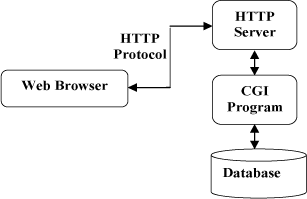
\includegraphics[scale=0.8]{CGIHandleWorkflow.png}
	\caption{URI、URL、URN关系图}
	\label{fig:CGIHandleWorkflow}
\end{figure}

CGI程序通过标准输入(STDIN)和标准输出(STDOUT)来进行输入输出。
此外CGI程序还通过环境变量来得到输入,操作系统提供了许多环境变量,
它们定义了程序的执行环境,应用程序可以存取它们。
Web服务器和CGI接口又另外设置了一些环境变量,用来向CGI程序传递一些重要的参数。
CGI的GET方法还通过环境变量QUERY-STRING向CGI程序传递Form中的数据。
CGI工作原理:每当客户请求CGI的时候,WEB服务器就请求操作系统生成一个新的CGI解释器进程(如php-cgi.exe),
CGI 的一个进程则处理完一个请求后退出,下一个请求来时再创建新进程。
当然,这样在访问量很少没有并发的情况也行。可是当访问量增大,并发存在,
这种方式就不适合了。于是就有了FastCGI。FastCGI像是一个常驻(long-live)型的CGI,
它可以一直执行着,只要激活后,不会每次都要花费时间去fork一次(这是CGI最为人诟病的fork-and-execute模式)。
一般情况下,FastCGI的整个工作流程是这样的:

1.Web Server启动时载入FastCGI进程管理器(IIS ISAPI或Apache Module)

2.FastCGI进程管理器自身初始化,启动多个CGI解释器进程(可见多个php-cgi)并等待来自Web Server的连接。

3.当客户端请求到达Web Server时,FastCGI进程管理器选择并连接到一个CGI解释器。
Web server将CGI环境变量和标准输入发送到FastCGI子进程php-cgi。

4.FastCGI子进程完成处理后将标准输出和错误信息从同一连接返回Web Server。
当FastCGI子进程关闭连接时, 请求便告处理完成。
FastCGI子进程接着等待并处理来自FastCGI进程管理器(运行在Web Server中)的下一个连接。 
在CGI模式中,php-cgi在此便退出了。

PHP-FPM与Spawn-FCGI

Spawn-FCGI是一个通用的FastCGI管理服务器,它是lighttpd中的一部份,
很多人都用Lighttpd的Spawn-FCGI进行FastCGI模式下的管理工作。
但是有缺点,于是PHP-fpm就是针对于PHP的,Fastcgi的一种实现,
他负责管理一个进程池,来处理来自Web服务器的请求。
目前,PHP-fpm是内置于PHP的\footnote{http://www.cnblogs.com/liuzhang/p/3929198.html\#undefined}。

\subsection{MIME}

MIME(Multipurpose Internet Mail Extensions)多用途互联网邮件扩展类型。
是设定某种扩展名的文件用一种应用程序来打开的方式类型,
当该扩展名文件被访问的时候,浏览器会自动使用指定应用程序来打开。
多用于指定一些客户端自定义的文件名,以及一些媒体文件打开方式。
它是一个互联网标准,扩展了电子邮件标准,使其能够支持:
非ASCII字符文本;非文本格式附件(二进制、声音、图像等);
由多部分(multiple parts)组成的消息体;
包含非ASCII字符的头信息(Header information)。
这个标准被定义在RFC\footnote{Request For Comments(RFC),
是一系列以编号排定的文件。文件收集了有关互联网相关信息,
以及UNIX和互联网社区的软件文件。
目前RFC文件是由Internet Society(ISOC)赞助发行。
基本的互联网通信协议都有在RFC文件内详细说明。RFC文件还额外加入许多的论题在标准内,
例如对于互联网新开发的协议及发展中所有的记录。
因此几乎所有的互联网标准都有收录在RFC文件之中。} 2045、RFC 2046、RFC 2047、RFC 2048、RFC 2049等RFC中。 
MIME改善了由RFC 822转变而来的RFC 2822,
这些旧标准规定电子邮件标准并不允许在邮件消息中使用7位ASCII字符集以外的字符。
正因如此,一些非英语字符消息和二进制文件,
图像,声音等非文字消息原本都不能在电子邮件中传输(MIME可以)。
Internet中有一个专门组织IANA(The Internet Assigned Numbers Authority)\footnote{IANA(The Internet Assigned Numbers Authority,
互联网数字分配机构)是负责协调一些使Internet正常运作的机构。
同时,由于Internet已经成为一个全球范围的不受集权控制的全球网络,
为了使网络在全球范围内协调,存在对互联网一些关键的部分达成技术共识的需要,
而这就是IANA的任务。}来确认标准的MIME类型,
但Internet发展的太快,很多应用程序等不及IANA来确认他们使用的MIME类型为标准类型。
因此他们使用在类别中以x-开头的方法标识这个类别还没有成为标准,例如:x-gzip,x-tar等。
MIME规定了用于表示各种各样的数据类型的符号化方法。 
此外,在万维网中使用的HTTP协议中也使用了MIME的框架,标准被扩展为互联网媒体类型。
MINE中的Content-Type表明信息类型,缺省值为" text/plain"。
它包含了主要类型(primary type)和次要类型(subtype)两个部分,
两者之间用"/"分割。主要类型有9种,
分别是application、audio、example、image、message、model、multipart、text、video。
每一种主要类型下面又有许多种次要类型,常见的有:

\begin{lstlisting}
text/plain:纯文本,文件扩展名.txt
text/html:HTML文本,文件扩展名.htm和.html
image/jpeg:jpeg格式的图片,文件扩展名.jpg
image/gif:GIF格式的图片,文件扩展名.gif
audio/x-wave:WAVE格式的音频,文件扩展名.wav
audio/mpeg:MP3格式的音频,文件扩展名.mp3
video/mpeg:MPEG格式的视频,文件扩展名.mpg
application/zip:PK-ZIP格式的压缩文件,文件扩展名.zip
\end{lstlisting}

常见的MIME类型对照表如表\ref{table:MineType}所示,
详细的MIME类型对照表参见\url{http://tool.oschina.net/commons}。

\begin{table}\caption[Caption for LOF]{常用MIME类型对照表}\label{table:MineType}					
	\medskip
	\centering		
	\begin{tabular}{|c|c|}
		\hline
		\multirow{1}{*}{文件扩展名}		
		& \multicolumn{1}{c|}{Content-Type(Mime-Type)}\\			
		\cline{1-2}
		 .*( 二进制流,不知道下载文件类型) &  application/octet-stream\\
		\hline
		.mp4 & video/mpeg4\\
		\hline		
	\end{tabular}
\end{table}

\subsubsection{ashx}

一般处理程序(HttpHandler)是·NET众多web组件的一种,ashx是其扩展名。
一个HttpHandler接受并处理一个http请求,类比于Java中的servlet。
类比于在Java中需要继承HttpServlet类。在net中需要实现IHttpHandler接口,
这个接口有一个IsReusable成员,一个待实现的方法ProcessRequest(HttpContextctx)。
程序在processRequest方法中处理接受到的Http请求。
成员IsReusable指定此IhttpHandler的实例是否可以被用来处理多个请求。
.ashx程序适合产生供浏览器处理的、不需要回发处理的数据格式,
例如用于生成动态图片、动态文本等内容。

\begin{quotation}
Generic Web handler (*.ashx, extension based processor) is the default 
HTTP handler for all Web handlers that do not have a UI and that include the @WebHandler directive. 
\end{quotation}

其实用.aspx文件可以完全实现.ashx的功能,.ashx比着.aspx的优点是性能高一些,
它免去了.aspx页面的控件解析以及页面处理过程。它特别适合于生成动态图片,
生成动态文本之类,实现某一具体功能的操作。
平时查看ashx双击时Visual Studio自动定位到ashx.cs文件,
如果想要查看ashx文件本身的内容可选中文件点击鼠标右键,
有一个“查看标记”的菜单,点击即显示ashx文件本身的内容。
如下代码片段所示:

\begin{lstlisting}[language=HTML]
<%@ WebHandler Language="C#" CodeBehind="basics.ashx.cs" Class="XINLG.Weixin._codes.my.basics" %>
\end{lstlisting}


\subsubsection{cshtml}

Razor is a view engine for ASP.NET MVC, 
and also a template engine. Razor code and ASP.NET
 inline code (code mixed with markup) both get compiled 
 first and get turned into a temporary assembly before 
 being executed. Thus, just like C\# and VB.NET both compile to 
 IL which makes them interchangable, 
 Razor and Inline code are both interchangable. 

\subsection{虚拟目录(Virtual Directories)}

\begin{quotation}
A virtual directory is a directory name (also referred to as path) that you specify in IIS and map to a physical directory on a local or remote server. The directory name then becomes part of the application's URL, and users can request the URL from a browser to access content in the physical directory, such as a Web page or a list of additional directories and files. If you specify a different name for the virtual directory than the physical directory, it is more difficult for users to discover the actual physical file structure on your server because the URL does not map directly to the root of the site.

In IIS 7 and above, each application must have a virtual directory, which is named the root virtual directory, and which maps the application to the physical directory that contains the application's content. However, an application can have more than one virtual directory. For example, you might use a virtual directory when you want your application to include images from another location in the file system, but you do not want to move the image files into the physical directory that is mapped to the application's root virtual directory.

By default, IIS uses configuration from Web.config files in the physical directory to which the virtual directory is mapped, as well as in any child directories in that physical directory. If you do not want to use Web.config files in child directories, specify false for the allowSubDirConfig attribute on the virtual directory.

Optionally, when you need to specify credentials and a method to access the virtual directory, you can specify values for the username, password, and logonMethod attributes. 
\end{quotation}

虚拟目录\footnote{http://www.iis.net/learn}可将大量的静态内容独立到一个系统盘符,
构建简单的分布应用。
可网络节点分布,提升硬盘IO性能。
可以映射到网络不同的硬盘,要知道IO的瓶颈,
就是单块硬盘的极限,通过映射到不同的硬盘,
性能的提升点就是:单块硬盘的极限*N块硬盘。
而这一切的扩展,只是简单的虚拟目录映射,
再移动相应的文件,而程序上,并不需要动刀,
简单就完成文件的分布式存储。
可以横向扩展,可以通过不停的加独立硬盘,
方便性的提升性能。

\section{HTTP}

\subsection{浏览器的请求流程}

\paragraph{DNS解析}导航的第一步是通过访问的域名找出其IP地址,
浏览器请求DNS查询到www.taobao.com对应的IP,
浏览器向对应的IP服务器发起TCP连接,
通过建立的TCP连接发送HTTP协议报文,
服务器发送响应,浏览器展现返回的内容。

\paragraph{301重定向}为什么服务器一定要重定向而不是直接发会用户想看的网页内容呢?这个问题有好多有意思的答案。
其中一个原因跟搜索引擎排名有 关。你看,如果一个页面有两个地址,
就像http://www.igoro.com/ 和http://igoro.com/,搜索引擎会认为它们是两个网站,
结果造成每一个的搜索链接都减少从而降低排名。而搜索引擎知道301永久重定向是什么意思,
这样就会把访问带www的和不带www的地址归到同一个网站排名下。
还有一个是用不同的地址会造成缓存友好性变差。当一个页面有好几个名字时,它可能会在缓存里出现好几次。

\subsection{完整的HTTP请求流程}

HTTP通信机制是在一次完整的HTTP通信过程中,
Web浏览器与Web服务器之间将完成下列7个步骤,
此处只是介绍高层的步骤,具体的细节需更多篇幅:

\begin{enumerate}
\setcounter{enumi}{0}
\item{建立TCP连接}~~
在HTTP工作开始之前,Web浏览器首先要通过网络与Web服务器建立连接,
该连接是通过TCP来完成的,该协议与IP协议共同构建Internet,
即著名的TCP/IP协议族,因此Internet又被称作是TCP/IP网络。
HTTP是比TCP更高层次的应用层协议,根据规则,
只有低层协议建立之后才能进行更高层协议的连接,
因此,首先要建立TCP连接,一般TCP连接的端口号是80。
建立TCP连接需要经过“3次握手(Three-way Handshake)”,具体如下:

\begin{itemize}
\item{SYN\_SEND}
客户端发送一个带SYN(seq=j,这里j的值为0)标志的TCP报文到服务器,
并进入SYN\_SEND状态,等待服务器确认,这是三次握手过程中的报文1,
如图所示。

\item{SYN\_RECV}
服务器收到syn包,必须确认客户的SYN(ack=j+1),
同时自己也发送一个SYN包(syn=k),即SYN+ACK包,此时服务器进入状态。

\item{ESTABLISHED}
客户端收到服务器的SYN+ACK包,
向服务器发送确认包ACK(ack=k+1),
此包发送完毕,客户端和服务器进入ESTABLISHED状态,
完成三次握手。

\begin{figure}[htbp]
	\centering
	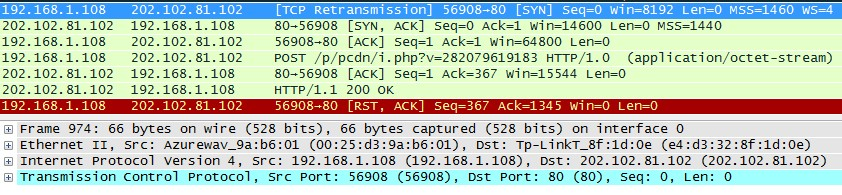
\includegraphics[scale=0.7]{TCPThreeHanding.jpg}
	\caption{TCP3次握手}
	\label{fig:TCPThreeHanding}
\end{figure}

\end{itemize}

\item{Web浏览器向Web服务器发送请求命令}~~
一旦建立了TCP连接,Web浏览器就会向Web服务器发送请求命令。
例如:GET/sample/hello.jsp HTTP/1.1。

\item{Web浏览器发送请求头信息}~~
浏览器发送其请求命令之后,还要以头信息的形式向Web服务器发送一些别的信息,
之后浏览器发送了一空白行来通知服务器,它已经结束了该头信息的发送。

\item{Web服务器应答}~~
客户机向服务器发出请求后,服务器会客户机回送应答, HTTP/1.1 200 OK ,
应答的第一部分是协议的版本号和应答状态码。
服务器最基本的功能就是响应客户端的资源请求。
服务器首先会侦听80端口,来了http请求,
就根据请求进行处理,请求一个图片那就根据路径找到资源发回,
请求静态html页面也是如此,
如果请求的是像php这样的动态页面应该先调用php编译器(或是解释器吧)生成html代码,然后返回给客户端。

\item{Web服务器发送应答头信息}~~
正如客户端会随同请求发送关于自身的信息一样,
服务器也会随同应答向用户发送关于它自己的数据及被请求的文档。

\item{Web服务器向浏览器发送数据}~~
Web服务器向浏览器发送头信息后,它会发送一个空白行来表示头信息的发送到此为结束,
接着,它就以Content-Type应答头信息所描述的格式发送用户所请求的实际数据。

\item{Web服务器关闭TCP连接}~~
一般情况下,一旦Web服务器向浏览器发送了请求数据,
它就要关闭TCP连接,
然后如果浏览器或者服务器在其头信息加入了这行代码:Connection:keep-alive
TCP连接在发送后将仍然保持打开状态,于是,浏览器可以继续通过相同的连接发送请求。
保持连接节省了为每个请求建立新连接所需的时间,还节约了网络带宽。
从HTTP/1.1起,默认都开启了Keep-Alive,保持连接特性,
简单地说,当一个网页打开完成后,
客户端和服务器之间用于传输HTTP数据的TCP连接不会关闭,
如果客户端再次访问这个服务器上的网页,会继续使用这一条已经建立的连接。
Keep-Alive不会永久保持连接,它有一个保持时间,
可以在不同的服务器软件(如Apache)中设定这个时间,
IIS 7默认是120秒。
\end{enumerate}


\subsection{Http请求在IIS中的处理流程}

进入的HTTP Web请求最先由IIS Web服务器接收到,
它在此请求基于ASP.NET已注册处理的扩展名传送到ASP.NET ISAPI上。
HTTP运行期首先创建一个HttpContext对象的实例,HttpContext类由HttpRuntime对象实例化,
接着该对象会经历请求生存期的各个阶段,它包含了当前正在处理的请求信息,
接着创建在处理逻辑中涉及到的所有其他组件都可以使用的上下文对象。
HttpContext实例提供了对请求对象(HttpRequest类的实例)和响应对象(HttpResponse类的实例)的访问。

\paragraph{IIS 7.0}
在Kernel Mode下,http.sys接收到一个基于Aspx的HttpRequest,
然后它会根据IIS中的Metabase查看该基于该Request的Application属于哪个Application Pool,
如果该Application Pool不存在,则创建之。否则直接将request发到对应Application Pool的Queue中。
每个Application Pool对应着一个Worker Process:w3wp.exe,毫无疑问他是运行在User Mode下的。
在IIS Metabase中维护着Application Pool和worker process的Mapping。
WAS(Web Administrative service)根据这样一个mapping,
将存在于某个Application Pool Queue的request 传递到对应的worker process(如果没有,就创建这样一个进程)。
在worker process初始化的时候,加载ASP.NET ISAPI,ASP.NET ISAPI进而加载CLR。
最后的流程就和IIS 5.x一样了:通过AppManagerAppDomainFactory的Create方法为Application创建一个Application Domain;
通过ISAPIRuntime的ProcessRequest处理Request,进而将流程进入到ASP.NET Http Runtime Pipeline。

\subsection{HttpRuntime}

Asp.net有四大核心对象:HttpContext, HttpRequest, HttpResponse,HttpRuntime。
IIS 所收到的对某 Microsoft ASP.NET 页面的每个请求都被移交给 ASP.NET HTTP 管线(Pipline)。
HTTP 管线由一系列托管对象组成,这些对象按顺序处理该请求,
并完成从URL到普通HTML文本的转换。
HTTP管线的入口点是 HttpRuntime 类。
ASP.NET基础结构为辅助进程中所承载的每个AppDomain创建此类的一个实例请注意,
该辅助进程为当前正在运行的每个 ASP.NET 应用程序维护一个不同的 AppDomain。

要激活HTTP管道,可以创建一个HttpRuntime类的新实例,
然后调用其ProcessRequest方法。一个完整的页面请求会包括下面的流程:
首先被WWW服务器截获(inetinfo.exe进程), 该进程首先判断页面后缀, 
然后根据IIS中配置决定调用具体的扩展程序。aspx就会调用aspnet\_isapi.dll, 
然后由aspnet\_isapi.dll发送给w3wp.exe(iis 工作者进程,IIS6.0中叫做 w3wq.exe,
IIS5.0中叫做 aspnet\_wp.exe)。
接下来在w3wp.exe调用.NET类库进行具体处理,顺序如下:
ISAPIRuntime, HttpRuntime, HttpApplicationFactory, HttpApplication, 
HttpModule, HttpHandlerFactory, HttpHandler。

ISAPIRuntime:主要作用是调用一些非托管代码生成HttpWorkerRequest对象,
HttpWorkerRequest对象包含当前请求的所有信息,然后传递给HttpRuntime

HttpRuntime:根据HttpWorkerRequest对象生成HttpContext,HttpContext包含request、response等属性, 
HttpRuntime初始化HttpContext如代码片段\ref{code:InitialHttpContext}所示。

\begin{lstlisting}[language={[Sharp]C},caption=初始化HttpContext,label={code:InitialHttpContext}]
private void ProcessRequestInternal(HttpWorkerRequest wr)
{
  HttpContext context;
  try
  {
    context = new HttpContext(wr, false);
  }
  catch
  {
    wr.SendStatus(400, "Bad Request");
    wr.SendKnownResponseHeader(12, "text/html; charset=utf-8");
    byte[] bytes = Encoding.ASCII.GetBytes("<html><body>Bad Request</body></html>");
    wr.SendResponseFromMemory(bytes, bytes.Length);
    wr.FlushResponse(true);
    wr.EndOfRequest();
    return;
  }
}
\end{lstlisting}

400 Bad Request是客户端请求与语法错误,不能被服务器所理解,
无法正确初始化HttpContext。初始化HttpRuntime完成后再调用HttpApplicationFactory来生成IHttpHandler, 
调用HttpApplication对象执行请求

HttpApplicationFactory:生成一个HttpApplication对象,
如代码片段\ref{code:GenerateHttpApplicationObject}所示。

\begin{lstlisting}[language={[Sharp]C},caption=生成HttpApplication,label={code:GenerateHttpApplicationObject}]
IHttpHandler applicationInstance = HttpApplicationFactory.GetApplicationInstance(context);
if (applicationInstance == null)
  throw new HttpException(SR.GetString("Unable_create_app_object"));
\end{lstlisting}

HttpApplication:进行HttpModule的初始化,
HttpApplication创建针对此Http请求的 HttpContext对象HttpModule: 
当一个HTTP请求到达HttpModule时,整个ASP.NET Framework系统还并没有对这个HTTP请求做任何处理,
也就是说此时对于HTTP请求来讲,HttpModule是一个HTTP请求的“必经之路”,
所以可以在这个HTTP请求传递到真正的请求处理中心(HttpHandler)之前附加一些需要的信息在这个HTTP请求信息之上,
或者针对截获的这个HTTP请求信息作一些额外的工作,或者在某些情况下干脆终止满足一些条件的HTTP请求,
从而可以起到一个Filter过滤器的作用。

HttpHandlerFactory:把用户request 转发到HttpHandlerFactory,
再由HttpHandlerFactory实例化HttpHandler对象。

HttpHandle:Http处理程序,处理页面请求。
从上面看出HttpRuntime其中有一个ProcessRequest 方法
public static void ProcessRequest(HttpWorkerRequest wr);  //驱动所有 ASP.NET Web 处理执行。

\subsection{HttpContext}

HttpContext基于HttpApplication的处理管道,由于 HttpContext对象贯穿整个处理过程,
所以,可以从HttpApplication处理管道的前端将状态数据传递到管道的后端,完成状态的传递任务。
HttpContext的生命周期从服务器接收的HTTP请求开始到反应发送回客户端结束。
在WebForm或类库(包括MVC)项目中,通过Current静态属性,就能够获得HttpContext的对象。
在MVC的Controller中使用的Request实际上是HttpContext的Request属性。

\begin{lstlisting}[language={[Sharp]C}]
//输出:/Home/Index
string rawUrl = Request.RawUrl;
//输出:localhost
string host = Request.Url.Host;
//输出:http://localhost/Home/Index
string concatUrl = "http://" + host + rawUrl;
//输出:http://localhost:57699/Home/Index
string url = Request.Url.ToString();
//输出:http://localhost:57699/Home/Index
string originalString = Request.Url.OriginalString;
\end{lstlisting}


\subsection{HttpModule}

HttpModule是类似于过滤器的作用,可以没有,也可以有任意个,
每一个都可以订阅管道事件中的任意个事件,在每个订阅的事件中可自定义功能实现。
由于HttpModule的个数可以有多个,
我们可以定义HttpModule实现类,
然后再web.config中增加配置项,就可以实现多个HttpModule同时订阅管道事件了。

HTTP模块是一个在每次针对应用程序发出请求时调用的程序集。
HTTP模块作为ASP.NET请求管道的一部分调用,
它们能够在整个请求过程中访问生命周期事件。
HTTP模块使您可以检查传入和传出的请求并根据该请求进行操作。
HTTP 模块通常具有以下用途:

\begin{itemize}
\item{\textbf{安全}}
您可以检查传入的请求,
所以HTTP模块可以在调用请求页、XML Web Services或处理程序之前执行自定义的身份验证或其他安全检查。
\item{\textbf{统计信息和日志记录}}
HTTP模块是在每次请求时调用的,所以,
您可以将请求统计信息和日志信息收集到一个集中的模块中,而不是收集到各页中。
\item{\textbf{自定义的页眉或页脚}}
您可以修改传出响应,
所以可以在每一个页面或XML Web Services响应中插入内容,如自定义的标头信息。
\end{itemize}

\subsection{HttpHandler}
 
HttpHandler是HTTP请求的处理中心,
真正地对客户端请求的服务器页面做出编译和执行,
并将处理过后的信息附加在HTTP请求信息流中再次返回到HttpModule中。  
HttpHandler与HttpModule不同,
一旦定义了自己的HttpHandler类,
那么它对系统的HttpHandler的关系将是“覆盖”关系。 
 
\subsection{HTTP结构}

HTTP协议大家都知道是规定了以ASCII码传输,
建立在TCP、IP协议之上的应用层规范,
规范内容把HTTP请求分为3个部门:状态行,请求头,请求体。
所有的方法、实现都是围绕如何运用和组织这三部分来完成的。
HTTP使用统一资源标识符(Uniform Resource Identifiers, URI)来传输数据和建立连接。
一旦建立连接后,
数据消息就通过类似Internet邮件所使用的格式[RFC5322]和多用途Internet邮件扩展(MIME)[RFC2045]来传送。
客户端发送一个HTTP请求到服务器的请求消息包括以下格式:
请求行(request line)、请求头部(header)、空行和请求数据4个部分组成,
一个简单的请求如下代码片段所示:

\begin{lstlisting}[language=HTML]
GET /hello.txt HTTP/1.1`\makeremark{此行为状态行,依次为请求的方法、请求的资源、协议版本,接下来几行的内容为请求头,请求头以Key-Value的形式展现,也可以添加自定义请求头,例如在需要授权认证的Api中将加密信息添加到请求头中}`
User-Agent: curl/7.16.3 libcurl/7.16.3 OpenSSL/0.9.7l zlib/1.2.3`\makeremark{User-Agent头域的内容包含发出请求的用户信息}`
Host: www.example.com`\makeremark{Host头域指定请求资源的Intenet主机和端口号,必须表示请求url的原始服务器或网关的位置。HTTP/1.1请求必须包含主机头域,否则系统会以400状态码返回}`
Accept-Language: en, mi
\end{lstlisting}

\showremarks

HTTP的头域包括通用头、请求头、响应头和实体头四个部分。
每个头域由一个域名,冒号(:)和域值三部分组成。
通用头部是客户端和服务器都可以使用的头部,
可以在客户端、服务器和其他应用程序之间提供一些非常有用的通用功能,如Date头部。
请求头部是请求报文特有的,它们为服务器提供了一些额外信息,
比如客户端希望接收什么类型的数据,如Accept头部。
响应头部便于客户端提供信息,
比如,客服端在与哪种类型的服务器进行交互,如Server头部。
实体头部指的是用于应对实体主体部分的头部,
比如,可以用实体头部来说明实体主体部分的数据类型,如Content-Type头部。

\subsubsection{HTTP Header}

\paragraph{通用头(General Header Fields)}

通用头域包含请求和响应消息都支持的头域,
通用头域包含缓存头部Cache-Control、Pragma及信息性头部Connection、Date、Transfer-Encoding、Update、Via。

1、Cache-Control

Cache-Control指定请求和响应遵循的缓存机制。
在请求消息或响应消息中设置Cache-Control并不会修改另一个消息处理过程中的缓存处理过程。
请求时的缓存指令包括no-cache、no-store、max-age、 max-stale、min-fresh、only-if-cached,
响应消息中的指令包括public、private、no-cache、no- store、no-transform、must-revalidate、proxy-revalidate、max-age。各个消息中的指令含义如下:

no-cache:指示请求或响应消息不能缓存,
实际上是可以存储在本地缓存区中的,
只是在与原始服务器进行新鲜度验证之前,
缓存不能将其提供给客户端使用。 

no-store:缓存应该尽快从存储器中删除文档的所有痕迹,
因为其中可能会包含敏感信息。

max-age:缓存无法返回缓存时间长于max-age规定秒的文档,
若不超规定秒浏览器将不会发送对应的请求到服务器,
数据由缓存直接返回;超过这一时间段才进一步由服务器决定是返回新数据还是仍由缓存提供。
若同时还发送了max-stale指令,则使用期可能会超过其过期时间。

min-fresh:至少在未来规定秒内文档要保持新鲜,
接受其新鲜生命期大于其当前 Age 跟 min-fresh 值之和的缓存对象。

max-stale:指示客户端可以接收过期响应消息,
如果指定max-stale消息的值,那么客户端可以接收过期但在指定值之内的响应消息。

only-if-cached:只有当缓存中有副本存在时,客户端才会获得一份副本。

Public:指示响应可被任何缓存区缓存,可以用缓存内容回应任何用户。

Private:指示对于单个用户的整个或部分响应消息,
不能被共享缓存处理,只能用缓存内容回应先前请求该内容的那个用户。

打开新窗口时,如果指定cache-control的值为private、no-cache、must-revalidate,
那么打开新窗口访问时都会重新访问服务器。
而如果指定了max-age值,那么在此值内的时间里就不会重新访问服务器,
例如:Cache-control: max-age=5表示当访问此网页后的5秒内再次访问不会去服务器。
在ASP中,可以通过Response对象的Expires、ExpiresAbsolute属性控制Expires值;
通过Response对象的CacheControl属性控制Cache-control的值,
例如:
Response.ExpiresAbsolute = \#2000-1-1\#'指定绝对的过期时间,
这个时间用的是服务器当地时间,会被自动转换为GMT时间
Response.Expires = 20' 指定相对的过期时间,
以分钟为单位,表示从当前时间起过多少分钟过期。
Response.CacheControl = "no-cache"
Expires值是可以通过在Internet临时文件夹中查看临时文件的属性看到的。

2、Pragma

Pragma头域用来包含实现特定的指令,最常用的是Pragma:no-cache。在HTTP/1.1协议中,它的含义和Cache- Control:no-cache相同。

3、Connection

Connection表示是否需要持久连接。如果Servlet看到这里的值为“Keep-Alive”,或者看到请求使用的是HTTP 1.1(HTTP 1.1默认进行持久连接),它就可以利用持久连接的优点,当页面包含多个元素时(例如Applet,图片),显著地减少下载所需要的时间。要实现这一点,Servlet需要在应答中发送一个Content-Length头,最简单的实现方法是:先把内容写入ByteArrayOutputStream,然后在正式写出内容之前计算它的大小。

Close:告诉WEB服务器或者代理服务器,在完成本次请求的响应后,断开连接,不要等待本次连接的后续请求了。

Keepalive:告诉WEB服务器或者代理服务器,在完成本次请求的响应后,保持连接,等待本次连接的后续请求。

Keep-Alive:如果浏览器请求保持连接,则该头部表明希望 WEB 服务器保持连接多长时间(秒),如Keep-Alive:300。

4、Date

Date头域表示消息发送的时间,服务器响应中要包含这个头部,因为缓存在评估响应的新鲜度时要用到,其时间的描述格式由RFC822定义。例如,Date:Mon, 31 Dec 2001 04:25:57 GMT。Date描述的时间表示世界标准时,换算成本地时间,需要知道用户所在的时区。

5、Transfer-Encoding

WEB 服务器表明自己对本响应消息体(不是消息体里面的对象)作了怎样的编码,比如是否分块(chunked),例如:Transfer-Encoding: chunked

6、Upgrade

它可以指定另一种可能完全不同的协议,如HTTP/1.1客户端可以向服务器发送一条HTTP/1.0请求,其中包含值为“HTTP/1.1”的Update头部,这样客户端就可以测试一下服务器是否也使用HTTP/1.1了。

7、Via

列出从客户端到 OCS 或者相反方向的响应经过了哪些代理服务器,他们用什么协议(和版本)发送的请求。

当客户端请求到达第一个代理服务器时,该服务器会在自己发出的请求里面添加 Via 头部,并填上自己的相关信息,当下一个代理服务器 收到第一个代理服务器的请求时,会在自己发出的请求里面复制前一个代理服务器的请求的Via头部,并把自己的相关信息加到后面,以此类推,当 OCS 收到最后一个代理服务器的请求时,检查 Via 头部,就知道该请求所经过的路由。例如:Via:1.0 236-81.D07071953.sina.com.cn:80 (squid/2.6.STABLE13)

\paragraph{请求头(Request Header Fields)}

\paragraph{响应头(Response Header Fields)}

\paragraph{实体头(Entity Header Fields)}

\subsection{HTTP协议-压缩(HTTP Protocol-Compress)}

HTTP压缩是指: Web服务器和浏览器之间压缩传输的“文本内容”的方法。
HTTP采用通用的压缩算法,比如gzip来压缩HTML,Javascript, CSS文件。
能大大减少网络传输的数据量,提高了用户显示网页的速度。当然,同时会增加一点点服务器的开销。
HTTP压缩,在HTTP协议中,其实是内容编码的一种。
在HTTP协议中,可以对内容(也就是body部分)进行编码,可以采用gzip这样的编码。
从而达到压缩的目的。 也可以使用其他的编码把内容搅乱或加密,以此来防止未授权的第三方看到文档的内容。
HTTP压缩,其实就是HTTP内容编码的一种,HTTP压缩和HTTP内容编码两个概念容易混淆。
HTTP定义了一些标准的内容编码类型,并允许用扩展的形式添加更多的编码。
Content-Encoding header 就用这些标准化的代号来说明编码时使用的算法。
Content-Encoding值:

\begin{tabular}{l|p{12cm}}
	\multirow{1}{*}{}			
	& \multicolumn{1}{c}{}\\
	gzip & 表明实体采用GNU zip编码\\
	compress & 表明实体采用Unix的文件压缩程序\\
	deflate & 表明实体是用zlib的格式压缩的\\
	identity & 表明没有对实体进行编码。当没有Content-Encoding header时, 就默认为这种情况\\
\end{tabular}

gzip,compress,以及deflate编码都是无损压缩算法,用于减少传输报文的大小,不会导致信息损失。
其中gzip通常效率最高,使用最为广泛。 HTTP压缩对纯文本可以压缩至原内容的40\%,从而节省了60\%的数据传输。 
Gzip压缩是在一个文本文件中找出类似的字符串, 并临时替换他们,使整个文件变小。
这种形式的压缩对Web来说非常适合, 因为HTML和CSS文件通常包含大量的重复的字符串,例如空格,标签。
浏览器在发送请求时告知可以接收的压缩编码类型,如图\ref{fig:BrowserAcceptCodingType}所示,
由图可知浏览器可接受的压缩编码类型为gzip,deflate,sdch。
现在最好禁用deflate压缩,因为现在浏览器对DEFLATE压缩处理不好,
早期浏览器对DEFLATE压缩描述混乱\footnote{http://www.webkaka.com/blog/archives/DEFLATE-Obsolete-Compression-Format.html},
deflate有可能直接穿过某些防火墙产品,
给骇客留下弱点。

\begin{figure}[htbp]
	\centering
	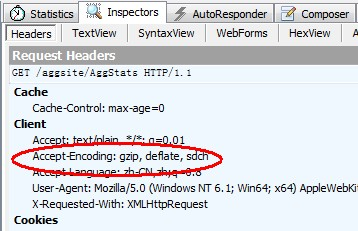
\includegraphics[scale=1]{HttpAcceptCompressEncoding.jpg}
	\caption{告知可接受的压缩编码类型}
	\label{fig:BrowserAcceptCodingType}
\end{figure}

在启用了gzip压缩的网站响应头中会有如下语句:

\begin{lstlisting}[language=HTML]
Content-Encoding: gzip
\end{lstlisting}

\subsection{HTTP ETag} 

ETag全称Entity Tag,用来标识一个资源。在具体的实现中,ETag可以是资源的hash值,
也可以是一个内部维护的版本号。但不管怎样,ETag应该能反映出资源内容的变化,这是Http缓存可以正常工作的基础。
在HTTP1.1规范中,新增了一个HTTP头信息:ETag。对Web开发者来说,它是一个非常重要的信息。
它是用作缓存使用的两个主要的头信息之一 (另一个是Expires)。除此之外,在REST架构中,
它还可以用于控制并发操作(上节中已经大致介绍AtomPub中控制并发的流程)。
ETag:是实体标签(Entity Tag)的缩写。ETag一般不以明文形式相应给客户端。
在资源的各个生命周期中,它都具有不同的值,用于标识出资源的状态。
当资源发生变更时,如果其头信息中一个或者多个发生变化,或者消息实体发生变化,
那么ETag也随之发生变化。在HTTP1.1协议中并没有规范如何计算ETag。
ETag值可以是唯一标识资源的任何东西,如持久化存储中的某个资源关联的版本、一个或者多个文件属性,
实体头信息和校验值、(CheckSum),也可以计算实体信息的散列值。有时候,
为了计算一个ETag值可能有比较大的代价,此时可以采用生成唯一值等方式(如常见的GUID)。
无论怎样,服务都应该尽可能的将ETag值返回给客户端。客户端不用关心ETag值如何产生,
只要服务在资源状态发生变更的情况下将ETag值发送给它就行。
OutgoingResponse类中设置ETag值如代码\ref{Code:GenerateETag}所示:

\begin{lstlisting}[language={[Sharp]C},caption=生成ETag,label={Code:GenerateETag}]
public void SetETag(string entityTag)
{
	this.ETag = OutgoingWebResponseContext.GenerateValidEtagFromString(entityTag);
}

public void SetETag(int entityTag)
{
	this.ETag = OutgoingWebResponseContext.GenerateValidEtag(entityTag);
}

public void SetETag(long entityTag)
{
	this.ETag = OutgoingWebResponseContext.GenerateValidEtag(entityTag);
}

public void SetETag(Guid entityTag)
{
	this.ETag = OutgoingWebResponseContext.GenerateValidEtag(entityTag);
}
\end{lstlisting}

在REST架构下,ETag值可以通过Guid、整数、长整形、字符串四种类型的参数传入SetETag方法,
WCF服务发回给客户端的HTTP响应头中就包含了ETag值。另外OutgoingResponse类也有字符串属性:
ETag直接给它赋值也能在HTTP响应头中写入ETag值。按照HTTP标准,Last-Modified只能精确到秒级。ETag的出现可以很好的解决这个问题。在用途上,ETag常与If-None-Match或者If-Match一起,
由客户端通过HTTP头信息(包括ETag值)发送给服务端处理。ETag有两种类型:
强ETag(strong ETag)与弱ETag(weak ETag)。

强ETag表示形式:"22FAA065-2664-4197-9C5E-C92EA03D0A16"。

弱ETag表现形式:w/"22FAA065-2664-4197-9C5E-C92EA03D0A16"。

强、弱ETag类型的出现与Apache服务器计算ETag的方式有关。
Apache默认通过FileEtag中FileEtag INode Mtime Size的配置自动生成ETag
(当然也可以通过用户自定义的方式)。假设服务端的资源频繁被修改(如1秒内修改了N次),
此时如果有用户将Apache的配置改为MTime,由于MTime只能精确到秒,
那么就可以避免强ETag在1秒内的ETag总是不同而频繁刷新Cache(如果资源在秒级经常被修改,
也可以通过Last-Modified来解决)

\subsection{HTTP Proxy}

Web代理(proxy)服务器是网络的中间实体。代理位于Web客户端和Web服务器之间,
扮演“中间人”的角色。HTTP的代理服务器即是Web服务器又是Web客户端。
Fiddler是以代理web服务器的形式工作的,它使用代理地址:127.0.0.1, 端口:8888.
当Fiddler退出的时候它会自动注销代理,这样就不会影响别的程序。

\begin{itemize}
\item{\textbf{代理翻墙}}~~很多人都喜欢用Facebook, 看YouTube。但是我们在天朝,天朝有The Great of Fire Wall(长城防火墙),屏蔽了这些好网站。怎么办?通过代理来跳墙,就可以访问了。
\item{\textbf{匿名访问}}~~经常听新闻,说“某某某”在网络上发布帖子,被跨省追缉了。
假如他使用匿名的代理服务器,就不容易暴露自己的身份了。HTTP代理服务器的匿名性是指: 
HTTP代理服务器通过删除HTTP报文中的身份特性(比如客户端的IP地址, 或cookie,或URI的会话ID),
从而对远端服务器隐藏原始用户的IP地址以及其他细节。 同时HTTP代理服务器上也不会记录原始用户访问记录的log(否则也会被查到)。
\item{\textbf{通过代理上网}}~~比如局域网不能上网, 只能通过局域网内的一台代理服务器上网。
\item{\textbf{代理缓存,加快上网速度}}~~大部分代理服务器都具有缓存的功能,就好像一个大的cache, 它有很大的存储空间,它不断将新取得数据存储到它本地的存储器上, 如果浏览器所请求的数据在它本机的存储器上已经存在而且是最新的,那么它就不重新从Web服务器取数据,而直接将存储器上的数据传给用户的浏览器,这样就能显著提高浏览速度。
\item{\textbf{儿童过滤器}}~~很多教育机构,会利用过滤器代理来阻止学生访问成人内容。
\end{itemize}

\subsection{HTTP Tunnel}

Http隧道分为两种:
1.不使用CONNECT的隧道
2.使用CONNECT的隧道

不使用CONNECT的隧道,实现了数据包的重组和转发。也就是在我们使用Proxy的时候,
然后发起Http请求,使用的就是非CONNECT的隧道。在这种情况下,在Proxy收到来自客户端的Http请求之后,
会重新创建Request请求,并发送到目标服务器,也就是图中的Content Server。
当目标服务器返回Response给Proxy之后,Proxy会对Response进行解析,然后重新组装Response,
发送给客户端。所以,在不使用CONNECT方式建立的隧道,Proxy有机会对客户端与目标服务器之间的通信数据进行窥探,
而且有机会对数据进行串改。

而对于使用CONNECT的隧道则不同。当客户端向Proxy发起Http CONNECT Method的时候,就是告诉Proxy,
先在Proxy和目标服务器之间先建立起连接,在这个连接建立起来之后,目标服务器会返回一个回复给Proxy,
Proxy将这个回复转发给客户端,这个Response是Proxy跟目标服务器连接建立的状态回复,
而不是请求数据的Response。在此之后,客户端跟目标服务器的所有通信都将使用之前建立起来的建立。
这种情况下的Http隧道,Proxy仅仅实现转发,而不会关心转发的数据。

这也是为什么在使用Proxy的时候,Https请求必须首先使用Http CONNECT建立隧道。
因为Https的数据都是经过加密的,Proxy是无法对Https的数据进行解密的,所以只能使用CONNECT,
仅仅对通信数据进行转发。

所以,实际上所有的网络库(例如libcurl, chromium\_net)在实现的时候,如果使用了Proxy,在请求Https协议的资源是,首先是使用CONNECT方法建立Http隧道,等收到目标服务器建立成功的回复之后,开始做SSL/TLS握手,然后进行数据传输。

虽然Http CONNECT隧道安全,能够使得客户端的数据实现"翻墙", 但是Http CONNECT容易失控,由于数据都是加密的,Proxy跟目标服务器建立TCP连接之后,之后的所有数据都服用这个连接。但是Http CONNECT隧道不仅仅是可以建立Https 443端口的连接,实际上可以建立任何端口的连接,这也使得Proxy变得非常危险,所以,一般的服务器都会对Http CONNECT隧道进行控制,只能实现Https 443端口的隧道通信。

\begin{figure}[htbp]
	\centering
	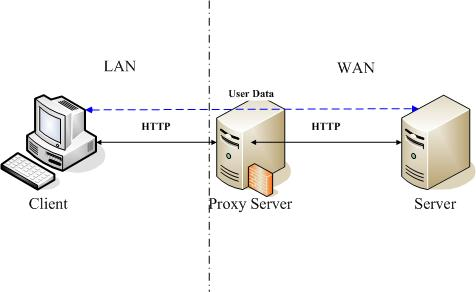
\includegraphics[scale=0.8]{HttpTunnel.jpg}
	\caption{HTTP隧道}
	\label{fig:HttpTunnel}
\end{figure}

HttpTuunnel(也叫Http隧道,Http穿梭),是这样一种技术: 
它用HTTP协议在要通信的Client和Server建立起一条“Tunnel”,
然后Client和Server之间的通信,都是在这条Tunnel的基础之上。
HttpTunnel通常被用在受限的网络环境中,
比如在NAT\footnote{Network Address Translation (NAT) is a methodology 
of remapping one IP address space into another by 
modifying network address information in Internet Protocol (IP) 
datagram packet headers while they are in transit across a 
traffic routing device.The technique was originally used for ease 
of rerouting traffic in IP networks without renumbering every host. 
It has become a popular and essential tool in conserving global 
address space allocations in face of IPv4 address exhaustion 
by sharing one Internet-routable IP address of a NAT gateway 
for an entire private network.}(Network address translation)环境中的Client,
受防火墙限制的环境中的Client等,
在这样的环境中,Client不能直接连接到公网(WAN)的Server,这时候就可以通过HttpTunnel技术,来解决上述问题。
上图是HttpTunnel技术的基本原理,它基本的工作过程主要分为以下几个步骤:
(1)Client向ProxyServer发送要连接到Server的请求(Http协议)
(2)Proxy Server向实际的Server发送连接请求(Http协议)
(3)上述两步成功后,就相当于在Client和Server之间存在了一条连通的Tunnel(如上图中的蓝色虚线所示)
(4)后续Client和Server就可以直接进行数据的收发,协议由Client和Server自己约定,与HttpTunnel无关

\subsection{REST方式POST、GET}

Get请求的数据会附在URL之后(就是把数据放在HTTP协议头中),
如果数据是英文字母或数字,原样发送,
如果是空格,转换为+,如果是中文或其他字符,
则直接把字符用BASE64加密,得到如:
\%E4\%BD\%A0\%E5\%A5\%BD类似格式,
其中\%XX中的X为该符号以16进制表示的ASCII.
GET方式通过在网络地址附加参数来完成数据的提交,
比如在地址http://www.google.com/webhp?hl=zh-CN中,
前面部分http://www.google.com/webhp表示数据提交的网址,
后面部分 hl=zh-CN 表示附加的参数,其中 hl表示一个键(key), 
zh-CN表示这个键对应的值(value)。POST把数据放置在HTTP包的包体中。
POST方式通过在页面内容中填写参数的方法来完成数据的提交,
参数的格式和 GET 方式一样,
是类似于 hl=zh-CN\&newwindow=1这样的结构。
程序代码如\ref{Code:RESTPostData}所示:

\begin{lstlisting}[language={[Sharp]C},caption=REST方式POST,不带验证,label={Code:RESTPostData}]
#region 从WCF接口POST数据-不带验证
/// <summary>  
/// POST请求与获取结果(带验证)  
/// </summary>  
/// <param name="url">请求的WCF地址</param>
/// <param name="postDataParam">请求参数集合(key=value\&key=value)</param>
public static string HttpPost(string url, string postDataParam,string authorization)
{
    string postUrl = url + (postDataParam == "" ? "" : "?") + postDataParam;
    HttpWebRequest request = (HttpWebRequest)WebRequest.Create(postUrl);
    request.Method = "POST";
    //添加验证
    request.Headers.Add("Authorization", authorization);
    byte[] bytes = Encoding.ASCII.GetBytes(postDataParam);
    request.ContentLength = bytes.Length;
    request.ContentType = "text/html;charset=UTF-8";
    Stream requestStream=request.GetRequestStream();
    requestStream.Write(bytes, 0, (int)bytes.Length);
    requestStream.Close();
    HttpWebResponse response = request.GetResponse() as HttpWebResponse;
    if (response != null)
    {
        Stream responseStream = response.GetResponseStream();
        if (responseStream != null)
        {
            StreamReader myStreamReader = new StreamReader(responseStream, Encoding.UTF8);
            resultString = myStreamReader.ReadToEnd();
            myStreamReader.Close();
            responseStream.Close();
        }
    }
    return resultString;
}
#endregion
\end{lstlisting}

Get请求浏览器或OS对其数据长度有限制,
太长的数据无法用Get操作.
POST服务器也有相应的限制.

1)IIS6的POST大小为200KB,
每个表单域100KB.

2)IIS6最大请求头16KB.

3)IIS6默认上传文件的大小是4MB.

服务端获取Get请求参数用Request.QueryString.
获取POST请求用Request.Form.
JSP用request.getParameter().
另POST的安全性比Get高.

\subsection{HTTP Request and HTTP Response}

一个HTTP请求报文由请求行(request line)、请求头部(header)、空行和请求数据4个部分组成。
HTTP协议的请求方法有GET、POST、HEAD、PUT、DELETE、OPTIONS、TRACE、CONNECT。
最常见的一种请求方式,当客户端要从服务器中读取文档时,
当点击网页上的链接或者通过在浏览器的地址栏输入网址来浏览网页的,
使用的都是GET方式。GET方法要求服务器将URL定位的资源放在响应报文的数据部分,
回送给客户端。使用GET方法时,请求参数和对应的值附加在URL后面,
利用一个问号(“?”)代表URL的结尾与请求参数的开始,传递参数长度受限制。
例如,/index.jsp?id=100\&op=bind,这样通过GET方式传递的数据直接表示在地址中,
所以我们可以把请求结果以链接的形式发送给好友。以用google搜索domety为例,
Request格式如下:

\begin{lstlisting}
GET /search?hl=zh-CN&source=hp&q=domety&aq=f&oq= HTTP/1.1  
Accept: image/gif, image/x-xbitmap, image/jpeg, image/pjpeg, application/vnd.ms-excel, application/vnd.ms-powerpoint, 
application/msword, application/x-silverlight, application/x-shockwave-flash, */*  
Referer: <a href="http://www.google.cn/">http://www.google.cn/</a>  
Accept-Language: zh-cn  
Accept-Encoding: gzip, deflate  
User-Agent: Mozilla/4.0 (compatible; MSIE 6.0; Windows NT 5.1; SV1; .NET CLR 2.0.50727; TheWorld)  
Host: <a href="http://www.google.cn">www.google.cn</a>  
Connection: Keep-Alive  
Cookie: PREF=ID=80a06da87be9ae3c:U=f7167333e2c3b714:
NW=1:TM=1261551909:LM=1261551917:S=ybYcq2wpfefs4V9g; 
NID=31=ojj8d-IygaEtSxLgaJmqSjVhCspkviJrB6omjamNrSm8lZhKy_
yMfO2M4QMRKcH1g0iQv9u-2hfBW7bUFwVh7pGaRUb0RnHcJU37y-
FxlRugatx63JLv7CWMD6UB_O_r  
\end{lstlisting}

可以看到,GET方式的请求一般不包含“请求内容”部分,
请求数据以地址的形式表现在请求行。地址链接如下:

\begin{lstlisting}[language=HTML]
<a href="http://www.google.cn/search?hl=zh-CN&source=hp&q=domety&aq=f&oq=">http://www.google.cn/search?hl=zh-CN&source=hp
&q=domety&aq=f&oq=</a> 
\end{lstlisting}

地址中”?”之后的部分就是通过GET发送的请求数据,
我们可以在地址栏中清楚的看到,各个数据之间用”\&”符号隔开。
显然,这种方式不适合传送私密数据。另外,
由于不同的浏览器对地址的字符限制也有所不同,
一般最多只能识别1024个字符,
服务器对地址字符同样也有相应的限制\footnote{具体可以 参考链接:
http://www.cnblogs.com/henryhappier/archive/2010/10/09/1846554.html},
为了让所有的用户都能正常浏览,我们的URL最好不要超过IE的最大长度限制(2038个字符),
当然,如果URL不直接提供给用户,而是提供给程序调用,侧这时的长度就只受Web服务器影响了。
所以如果需要传送大量数据的时候,也不适合使用GET方式。

\subsection{HTTP 状态码(HTTP Status Code)}

Response消息中的第一行叫做状态行,
由HTTP协议版本号,状态码,状态消息三部分组成。
状态码用来告诉HTTP客户端,HTTP服务器是否产生了预期的Response.
HTTP/1.1中定义了5类状态码,状态码由三位数字组成,第一个数字定义了响应的类别。

\subsubsection{2XX}

提示信息 - 表示请求已被成功接收,继续处理

2XX  成功 - 表示请求已被成功接收,理解,接受

\paragraph{204 No Content}HTTP的204(No Content)响应,就表示执行成功,但是没有数据, 浏览器不用刷新页面.也不用导向新的页面.当有一些服务,只是返回成功与否的时候,
可以尝试使用HTTP的状态码来作为返回信息,而省掉多余的数据传输,
比如REST中的DELETE和如上所述的查询式Ajax请求.

\paragraph{206 Partial Content}首先你需要知道文件大小以及远程服务器是否支持HTTP 206请求.使用curl命令可以查看任意资源的HTTP头,使用下面的curl命令可以发送一个HEAD请求:

\begin{lstlisting}[language=Bash]
curl -I http://192.168.1.222:8085/tour/images/beginPage_1.jpg

HTTP/1.1 200 OK
Content-Length: 311837
Content-Type: image/jpeg
Last-Modified: Fri, 22 Jan 2016 10:48:07 GMT
Accept-Ranges: bytes
ETag: "de59761255d11:0"
Server: Microsoft-IIS/7.5
X-Powered-By: ASP.NET
Date: Fri, 29 Jan 2016 08:44:21 GMT
\end{lstlisting}

Accept-Ranges: bytes -该响应头表明服务器支持Range请求,以及服务器所支持的单位是字节(这也是唯一可用的单位).
我们还能知道:服务器支持断点续传,以及支持同时下载文件的多个部分,
也就是说下载工具可以利用范围请求加速下载该文件.Accept-Ranges:none响应头表示服务器不支持范围请求.

Content-Length: 311837 - Content-Length响应头表明了响应实体的大小,
也就是真实的图片文件的大小是311837字节(304K).
服务器已经成功处理了部分GET请求。类似于FlashGet或者迅雷这类的HTTP
下载工具都是使用此类响应实现断点续传或者将一个大文档分解为多个下载段同时下载。
该请求必须包含 Range 头信息来指示客户端希望得到的内容范围,并且可能包含 If-Range
来作为请求条件。响应必须包含如下的头部域:Content-Range用以指示本次响应中返回的内容的范围;
如果是 Content-Type 为 multipart/byteranges 的多段下载,
则每一 multipart 段中都应包含Content-Range 域用以指示本段的内容范围。
假如响应中包含 Content-Length,那么它的数值必须匹配它返回的内容范围的真实字节数。
Date ETag 和/或 Content-Location,假如同样的请求本应该返回200响应。
Expires, Cache-Control,和/或 Vary,假如其值可能与之前相同变量的其他响应对应的值不同的话。
假如本响应请求使用了 If-Range 强缓存验证,那么本次响应不应该包含其他实体头;
假如本响应的请求使用了 If-Range 弱缓存验证,那么本次响应禁止包含其他实体头;
这避免了缓存的实体内容和更新了的实体头信息之间的不一致。否则,
本响应就应当包含所有本应该返回200响应中应当返回的所有实体头部域。
假如ETag或Last-Modified 头部不能精确匹配的话,
则客户端缓存应禁止将206响应返回的内容与之前任何缓存过的内容组合在一起。
任何不支持 Range 以及 Content-Range 头的缓存都禁止缓存206响应返回的内容。



\subsubsection{3XX}

\paragraph{301 Moved Permanently}301代表永久性转移(Permanently Moved),
301重定向是网页更改地址后对搜索引擎友好的最好方法,只要不是暂时搬移的情况,都建议使用301来做转址。

\paragraph{302 Found} Found:重定向,新的URL会在Response中的Location中返回,
浏览器将会自动使用新的URL发出新的Request。
例如在IE中输入, http://www.google.com. HTTP服务器会返回302, 
IE取到Response中Location header的新URL, 又重新发送了一个Request.
302代表暂时性转移(Temporarily Moved ),在前些年,不少Black Hat SEO曾广泛应用这项技术作弊。
各大主要搜索引擎均加强了打击力度,像Google对BMW德国网站的惩罚。
即使网站客观上不是spam,也很容易被搜寻引擎误判为spam而遭到惩罚。

\paragraph{304 Not Modified} Not Modified:代表上次的文档已经被缓存了, 还可以继续使用,
刷新一个网页时,Fiddler会捕获304类型的封包,
代表此资源可重复使用。

\subsubsection{4XX}

\paragraph{400}~ 400是一种是HTTP状态码,400 Bad Request。
是在打开网页时浏览器返回到客户端的一种状态码。显示在客户端的也就是400页面。
400页面是当用户在打开网页时,返回给用户界面带有400提示符的页面。
其含义是你访问的页面域名不存在或者请求错误。
主要有两种形式:
1、bad request意思是“错误的请求";
2、invalid hostname意思是"不存在的域名”。
通常只用Windows主机才会出现这样的字样,如果是Linux主机,会显示不同的错误提示。
bad request invalid hostname出现这个错误的原因是某个域名绑定到了某个主机上,
而该主机却没有绑定这个域名,所以IIS就返回了这个提示信息。

\paragraph{401}~一般来说该错误消息表明您首先需要登录(输入有效的用户名和密码)。
如果你刚刚输入这些信息,立刻就看到一个401错误,就意味着,
无论出于何种原因您的用户名和密码其中之一或两者都无效(输入有误,用户名暂时停用,等)。


4XX  客户端错误 - 请求有语法错误或请求无法实现。
400 Bad Request  客户端请求与语法错误,不能被服务器所理解。
403 Forbidden 服务器收到请求,但是拒绝提供服务。
404 Not Found 请求资源不存在(输错了URL)。
比如在IE中输入一个错误的URL, http://www.cnblogs.com/tesdf.aspx。

\subsubsection{5XX}

5XX  服务器端错误 - 服务器未能实现合法的请求。
500 Internal Server Error 服务器发生了不可预期的错误。
503 Server Unavailable 服务器当前不能处理客户端的请求,
一段时间后可能恢复正常。

\paragraph{503}服务不可用是的一种状态,那么在服务器503错误出现了之后,大家不必担心的, 服务器或许就是正在维护或者暂停了,你可以联系一下服务器空间商。还有的时候cpu占用的频率大导致的。
查看当前网站属于哪个应用程序,检查应用程序池是否处于停止状态。

\subsection{获取客户端IP}

\begin{lstlisting}[language={[Sharp]C}]
/// <summary>
/// 获取客户端ip
/// </summary>
/// <returns></returns>
public static string GetCurrentIP()
{
    string userHostAddress = string.Empty;
    try
    {
        ///如果客户端使用了代理服务器,则利用HTTP\_X\_FORWARDED\_FOR找到客户端IP地址
        userHostAddress = HttpContext.Current.Request.ServerVariables["HTTP_X_FORWARDED_FOR"].ToString().Split(',')[0].Trim();
        //否则直接读取REMOTE\_ADDR获取客户端IP地址
        if (string.IsNullOrEmpty(userHostAddress))
        {
            userHostAddress = HttpContext.Current.Request.ServerVariables["REMOTE_ADDR"];
        }
        //前两者均失败,则利用Request.UserHostAddress属性获取IP地址,但此时无法确定该IP是客户端IP还是代理IP
        if (string.IsNullOrEmpty(userHostAddress))
        {
            userHostAddress = HttpContext.Current.Request.UserHostAddress;
        }
        //最后判断获取是否成功,并检查IP地址的格式(检查其格式非常重要)
        if (!string.IsNullOrEmpty(userHostAddress) && IsIP(userHostAddress))
        {
            return userHostAddress;
        }
    }
    catch (Exception e)
    {
        logger.Error("Get current IP encount an error", e);
    }

    return userHostAddress;
}
\end{lstlisting}

在Web开发中,我们大多都习惯使用HTTP请求头中的某些属性来获取客户端的IP地址,
常见的属性是REMOTE\_ADDR、HTTP\_VIA和HTTP\_X\_FORWARDED\_FOR。
这三个属性的含义,大概是如此:REMOTE\_ADDR:该属性的值是客户端跟服务器“握手”时候的IP。
如果使用了“匿名代理”,REMOTE\_ADDR将显示代理服务器的IP。
X-Forwarded-For:
是用来识别通过HTTP代理或负载均衡方式连接到Web服务器的客户端最原始的IP地址的HTTP请求头字段。
X-Forwarded-For的有效性依赖于代理服务器提供的连接原始IP地址的真实性,
因此, X-Forwarded-For的有效使用应该保证代理服务器是可信的, 
比如可以通过建立可信服务器白名单的方式。

\subsection{placeholder属性}

placeholder属性是HTML5 中为input添加的。
在input上提供一个占位符,文字形式展示输入字段预期值的提示信息(hint),
该字段会在输入为空时显示。

\begin{lstlisting}[language=HTML]
<input type="text" name="UserName" class="form-control" placeholder="用户唯一ID"/>
\end{lstlisting}

\section{调试(Debug)}

WCF接口调试是在路由配置文件中设置,
传入适当的参数。如下所示:
\url{http://localhost:15973/ShowInfo/ShowAwardingListFC?openId=oM8-3t39DFln9lEdJCvUPAIHqbF8&accountId=34}。

页面的JavaScript脚本调试可以打开FireDebug,
打开脚本Tab页,在左侧的窗口中设置断点,
如图\ref{fig:FirefoxDebugPage}所示。
右侧的断点tab页可查看当前设置的所有断点。

\begin{figure}[htbp]
	\centering
	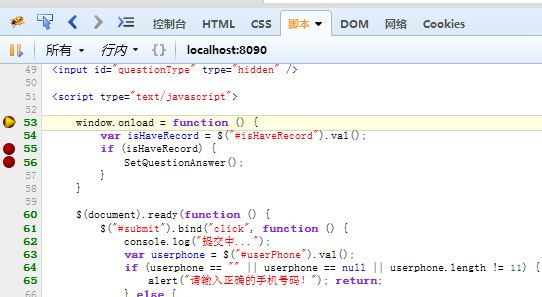
\includegraphics[scale=0.8]{FirefoxDebugPage.jpg}
	\caption{Firefox调试页面JavaScript脚本}
	\label{fig:FirefoxDebugPage}
\end{figure}

按F11进行单步进入调试,
按F12进行单步跳过调试。
在使用Visual Studio调试网页时,如果网页有微小的改动而你又不想重新启动新的调试界面,
那么可以利用Visual Studio的“浏览器链接(Browser Link)”功能,
如图\ref{fig:VisualStudioBrowserLink}所示,
每次启动页面时会在网页尾部添加一段Javascript脚本,
定时监听Visual Studio的刷新指令。

\begin{figure}[htbp]
	\centering
	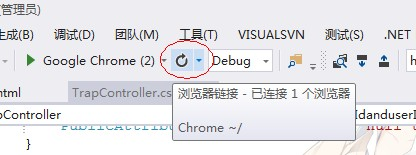
\includegraphics[scale=0.8]{VisualStudioBrowserLink.jpg}
	\caption{Visual Studio中刷新浏览器}
	\label{fig:VisualStudioBrowserLink}
\end{figure}

当修改页面之后只需要点击刷新符号,
链接到Visual Studio的浏览器即可即时刷新页面,
刷新链接浏览可以快速的看到页面修改结果,刷新是刷新链接浏览器的所有页面。
在调试MVC的Action时,没有View一样可以调试,
只需要浏览器链接指向Action即可,如果有参数带上相应参数。


\subsection{Chrome Javascript条件断点(Condition Breakpoint)}

在开发过程中Javascipt报空引用错误,
报错的地方有十几个循环,
在第7次循环是出现错误,那么此时需要快速定位错误的话,
条件断点是一个非常有用的助手。
在Google Chrome中按F12打开开发者调试工具,
在资源(Sources)下找到需要调试的Javascript脚本,
在断点位置的右键菜单中选择“Edit Breakpoint...”可以设置触发断点的条件,
就是写一个表达式,表达式为 true 时才触发断点,
此处是循环条件等于6。
新增条件断点如图\ref{fig:ConditionBreakpoints}所示,
当断点新增了条件之后,
断点标识的颜色会变为浅黄色(Google Chrome canary 48.0.2564.0(64-bit))。

\begin{figure}[htbp]
	\centering
	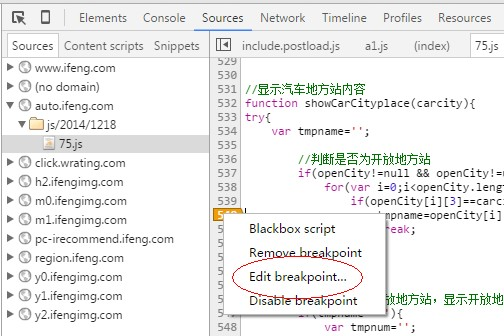
\includegraphics[scale=0.8]{ConditionBreakpoints.jpg}
	\caption{Javascript设置条件断点}
	\label{fig:ConditionBreakpoints}
\end{figure}

在调试Javascript时,
脚本有可能是经过压缩的,
此时显示仅有一行,为了便于阅读,
可点击调试器下方的大括号格式化压缩后的Javascript脚本,
如图\ref{fig:FormatZippedJavascript}所示。

\begin{figure}[htbp]
	\centering
	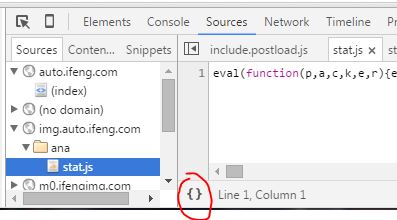
\includegraphics[scale=0.8]{FormatZippedJavascript.jpg}
	\caption{格式化Javascript脚本}
	\label{fig:FormatZippedJavascript}
\end{figure}

\subsection{SlidesJS改变滑动间隔}

使用SlideJS\footnote{SlidesJS is a responsive slideshow plug-in 
for jQuery (1.7.1+) with features like touch and CSS3 transitions. }
设置界面图片的滑动时间间隔如下代码所示:

\begin{lstlisting}
$("#slides").slidesjs({
			width: 1080,
			height: 500,
			play: 
			{
				auto:true,
				interval:10000
			}
		});
\end{lstlisting}

其中interval设置幻灯片的滑动的间隔时间,
单位为毫秒,这里设置的是10秒。

\subsection{IIS 6.0中MVC项目部署}

将MVC4网站部署到IIS6.0,部署完成后在网站的属性页面点击“配置”,
如图\ref{fig:IIS6MVC4ConfigAttribute}所示:

\begin{figure}[htbp]
	\centering
	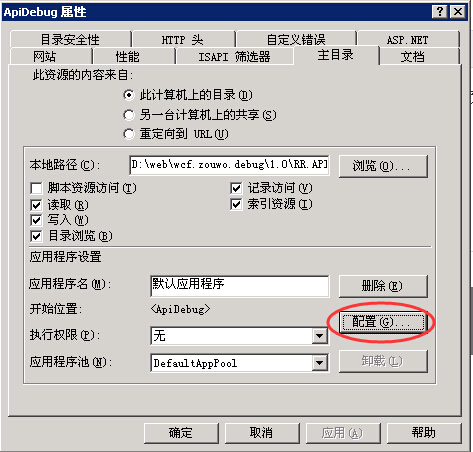
\includegraphics[scale=0.8]{IIS6MVC4ConfigAttribute.jpg}
	\caption{IIS6配置MVC4}
	\label{fig:IIS6MVC4ConfigAttribute}
\end{figure}

弹出的“应用程序配置”页面,映射下通配符应用程序映射中,
点击“插入”按钮,在弹出的界面中填写aspnet\_isapi.dll路径:

\begin{lstlisting}
C:\WINDOWS\Microsoft.NET\Framework64\v4.0.30319\aspnet_isapi.dll
\end{lstlisting}

如图\ref{fig:IIS6MVC4AppConfig}所示。注意需要将“确认文件是否存在”项勾选掉。
ISAPI(Internet Server Application Programming Interface)是一套本地的(Native)Win32 API,
是IIS和其他动态Web应用或平台之间的纽带。
ISAPI支持ISAPI扩展(ISAPI Extension)和ISAPI筛选(ISAPI Filter),
前者是真正处理HTTP请求的接口,
后者则可以在HTTP请求真正被处理之前查看、修改、转发或拒绝请求,
比如IIS可以利用ISAPI筛选进行请求的验证。
如果检测到某个HTTP请求的资源为静态资源(如:.html、.img、.text、.xml等),
IIS会将文件的内容直接响应给客户端,
对于动态资源(如:.aspx、.asp、.php等),
IIS则通过扩展名从IIS的脚本映射(Script Map)中找到相应的ISAPI动态链接库,
aspnet\_isapi.dll会被加载,
ASP.NET ISAPI随后会创建ASP.NET的工作进程。
IIS进程与工作进程间通过命名管道(Name Pipes)进行通信\cite{蒋金楠MVC框架揭秘}。

\begin{figure}[htbp]
	\centering
	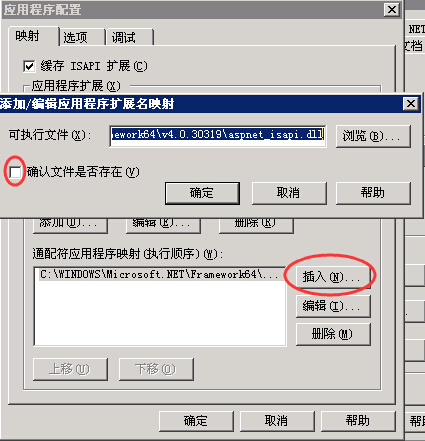
\includegraphics[scale=0.8]{IIS6MVC4AppConfig.jpg}
	\caption{IIS6配置MVC4应用程序配置}
	\label{fig:IIS6MVC4AppConfig}
\end{figure}

从以上叙述能够大致明白为什么需要手动配置aspnet\_isapi.dll。
需要注意的是,在添加aspnet\_isapi.dll路径时,尽量在“浏览”的弹出窗体中手动选择,
以避免复制粘贴时由于大小写等不一致造成问题。如果出现此问题:
Compilation Error: [No relevant source lines]。
那么可以设置应用程序池属性的标识选项卡中的预定义账户,
如图\ref{fig:AspNetAppPoolIdentitySetting}所示。
如果页面中提示403 Forbidden,可以将应用程序池标志中的预定义账户设置为“本地系统”。

\begin{figure}[htbp]
	\centering
	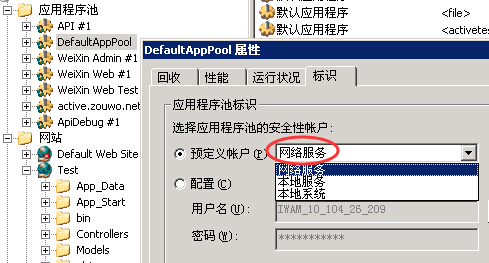
\includegraphics[scale=0.8]{AspNetAppPoolIdentitySetting.jpg}
	\caption{应用程序池标识设置}
	\label{fig:AspNetAppPoolIdentitySetting}
\end{figure}

在部署完毕后浏览网页时可能出现错误,如代码\ref{code:UserDefineError}所示进行设置,
可使IIS返回详细的错误信息,
便于进一步诊断错误。On 表示在本地和远程用户都会看到自定义错误信息。
Off 禁用自定义错误信息,本地和远程用户都会看到详细的错误信息。
RemoteOnly 表示本地用户将看到详细错误信息,而远程用户将会看到自定义错误信息。
当我们访问asp.net应用程时所使用的机器和发布asp.net应用程序所使用的机器为同一台机器时成为本地用户,
反之则称之为远程用户。在开发调试阶段为了便于查找错误Mode属性建议设置为Off,
而在部署阶段应将Mode属性设置为On或者RemoteOnly,
以避免这些详细的错误信息暴露了程序代码细节从而引来黑客的入侵。

\begin{lstlisting}[language=XML,caption=自定义错误设置,label={code:UserDefineError}]
<system.web>   
	<customErrors mode="Off">
	</customErrors> 
</system.web>
\end{lstlisting}

\subsection{HTML}

<span> 标签被用来组合文档中的行内元素(inline element),
也称作内联元素,例如:

\begin{lstlisting}[language=HTML]
<div class="content-text">今日剩余抽奖次数:<span id="lastCount"></span>次</div>
\end{lstlisting}

在这里span标签被用来替换页面中的可变元素。
span是一个标准的行内元素。
一个行内元素可以在段落中 <span> 像这样 </span> 包裹一些文字而不会打乱段落的布局。 
a元素是最常用的行内元素,它可以被用作链接。
与行类元素类似的是块级元素,
div是一个标准的块级元素。
一个块级元素会新开始一行并且尽可能撑满容器。
其他常用的块级元素包括p、form和HTML5中的新元素:header、footer、section等等。 

\begin{lstlisting}[language=HTML]
<form name="form" method="post">
    <center>
        <textarea id="code" name="qrcode" cols="60"></textarea>
    </center>
    <center>
        <input type="submit" class="btn btn-block btn-lg btn-danger" value="点击验证" />
    </center>
</form>
\end{lstlisting}

提交页面通过添加form标签,
指定form的method为post,
后台通过Request.Form["qrcode"]的形式接收参数,
其中qrcode为文本框的名称。

\subsection{AJax跨域请求}

获取服务器上面的打印数据的JavaScript代码:

\begin{lstlisting}[language=HTML]
function getPrintList(id, isRefresh) {
	var url = api_path + "/weixin/printdata?id=" + id;
	url += isRefresh ? "&an=refresh" : "";
	var obj = $(".print-list ul");
	$.ajax({
	    type: "get",
	    async: true,
	    url: url,
	    dataType: "jsonp",
	    jsonp: "callbackparam",
	    jsonpCallback: "success_jsonpCallback",
	    success: function (pjson) {
	        var tpl = '<li data-id="{guid}" step="{step}"><img src="' + api_path + '{url}" /><span></span><p>{date}</p></li>';
	        var lihtml = "";
	        json = pjson[0].newList;
	        if (pjson[0].count == 0) {
	            obj.html("<p class='info no-empty'>打印机空闲...</p>")
	            return;
	        }
	        for (var i = 0; i < json.length; i++) {
	            var waitingSeconds = i * print_speed;
	            var stime = ""
	            if (waitingSeconds >= 60 && waitingSeconds % 60 > 0) {
	                stime = waitingSeconds % 60 + "秒"
	            }
	            var time = waitingSeconds >= 60 ? parseInt(waitingSeconds / 60) + "分" + stime + "后" : waitingSeconds + "秒后";
	            if (waitingSeconds == 0) {
	                time = "请稍候...";
	            }
	            lihtml = tpl.replace("{url}", json[i].imageUrl).replace("{date}", time).replace("{guid}", json[i].guid).replace("{step}", json[i].step) + lihtml;
	        }
	        var printQueueNum = pjson[0].count - 1;
	        lihtml = '<li class="more"><p>......</p><span></span><p>共' + printQueueNum + '人排队</p></li>' + lihtml;  
	        obj.html(lihtml);
	        obj.find("li[step='5']").addClass("active").find("p").text("正在打印...");
	    },
	    error: function () {
	    }
	});
}
\end{lstlisting}

其中dataType为jsonp,JSONP(JSON with Padding)是一个非官方的协议,
它允许在服务器端集成Script tags返回至客户端,
通过javascript callback的形式实现跨域访问(这仅仅是JSONP简单的实现形式)。
由于同源策略\footnote{同源策略(Same Origin Policy)是一种约定,
它是浏览器最核心也最基本的安全功能,如果缺少了同源策略,
则浏览器的正常功能可能都会受到影响。可以说Web是构建在同源策略基础之上的,
浏览器只是针对同源策略的一种实现。所谓同源是指,域名,协议,端口相同。}的限制,
XmlHttpRequest只允许请求当前源(域名、协议、端口)的资源,
为了实现跨域请求,可以通过script标签实现跨域请求,
然后在服务端输出JSON数据并执行回调函数,从而解决了跨域的数据请求。

AJax\footnote{AJAX = Asynchronous JavaScript and XML(异步的 JavaScript 和 XML)。,
在2005年,Google通过其Google Suggest使AJax变得流行起来。}向后台提交数据,表单代码如下:

\begin{lstlisting}[language=HTML]
<div class="container">           
    <center style="margin-bottom:20px">
        <input type="tel" name="qrcode" id="qrcode" />
    </center>
    <center>
        <input id="inputbyhand" type="button" class="btn btn-block btn-lg btn-danger" onclick="btsave();" value="手动输入验证" />
    </center>
</div>
\end{lstlisting}

这里是当点击界面上手动输入按钮时,
通过POST方式将二维码值传入后台。
第一个input的type为tel时,
可以在移动端直接调出数字输入的界面。
第二个由onclick事件调取脚本中的btsave方法,
方法如下代码所示。

\begin{lstlisting}[language=VBScript]
function btsave() {
    var code = $("#qrcode").val();
    jQuery.ajax({
        url: '/my/qrcode',// 跳转到 action
        data: { "qrcode": code },
        type: 'post',
        cache: false,
        dataType: 'json',
        success: function (data) {                    
            alert(data.msg);
            $("#qrcode").val('');
        },
        error: function () {
            alert("异常!");
        }
    });
}
\end{lstlisting}

由于使用的是NVlocity模板,
aJax请求会与模板中的请求写法冲突,
所以此处的aJax请求写法为jQuery.ajax而不是\$.ajax,
获取后台的AjaxResult.msg返回信息用data.msg。

\subsection{文件上传}

\subsubsection{HTML5上传}

\begin{lstlisting}[language=HTML]
<form enctype="multipart/form-data" id="form1" action="~/QiuJiFangJiaoHui/OriginalUploadImage" method="post">
    <input type="hidden" id="userId" name="userId" value="@ViewData["userId"]" />
    <input type="hidden" id="activityId" name="activityId" value="@ViewData["activityId"]" />
    <div>
        <input type="file" style="width:220px;margin:20px auto;" id="userUploadFile" name="filename" accept="image/*" class='btn btn-warning' />
        <a href="#">
            <img id="userpic" onclick="sub();" src="http://static.zouwo.com/lottery/1.02/images/a16.jpg" style="width:100%">
        </a>
    </div>
</form>
\end{lstlisting}


\begin{lstlisting}[language={[Sharp]C}]
// 上传图片
public JsonResult OriginalUploadImage(int userId, int activityId)
{   
    Stream fileStream = Request.Files["filename"].InputStream;
}
\end{lstlisting}

\subsubsection{拖放上传}

此处的文件上传在MVC结构项目中实现,
拖放上传在服务器端的接收代码如片段所示。

\begin{lstlisting}[language={[Sharp]C}]
// 上传图片
public ActionResult Upload()
{
    try
    {
        var requestFiles = Request.Files`\makeremark{Gets the collection of files uploaded by the client, in multipart MIME format.The file collection is populated only when the HTTP request Content-Type value is "multipart/form-data".}`;
        foreach (string uploadFiles in requestFiles)
        {
            string filename = Guid.NewGuid() + ".jpg";
            string path = Path.Combine(Server.MapPath("~/App_Data"), filename);
            var requestFilesInstance = Request.Files[uploadFiles];
            if (requestFilesInstance != null)
            {
                requestFilesInstance.SaveAs(path);
                ViewBag.Message = "File(s) uploaded successfully";
            }
            else
            {
                _logger.Error("requestFilesInstance is null");
            }
        }
    }
    catch (Exception e)
    {
        _logger.Error("Upload file failed!", e);
    }

    return RedirectToAction("Index");
}
\end{lstlisting}

\showremarks

multipart/form-data的请求头必须包含一个特殊的头信息:
Content-Type,且其值也必须规定为multipart/form-data,
同时还需要规定一个内容分割符用于分割请求体中的多个post的内容,
内容分割符在Fiddler中捕获到如图\ref{fig:HTTPPostFileContentSplit}所示。

\begin{figure}[htbp]
	\centering
	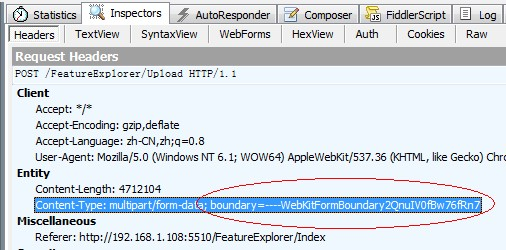
\includegraphics[scale=0.8]{HTTPPostFileContentSplit.jpg}
	\caption{multipart/form-data请求的内容分割符}
	\label{fig:HTTPPostFileContentSplit}
\end{figure}

从图中可以看出,分隔符的内容为:------WebKitFormBoundary2QnuIV0fBw76fRn7(Google Chrome Browser)。
在分隔符后就是原生的图片内容,如图\ref{fig:HTTPPostSplitWithRawData}所示。
图片数据流的最后以分隔符为标记。
multipart/form-data的请求体也是一个字符串,
不过和post的请求体不同的是它的构造方式,
post是简单的name=value值连接,
而multipart/form-data则是添加了分隔符等内容的构造体。
如文件内容和文本内容自然需要分割开来,不然接收方就无法正常解析和还原这个文件了。

\begin{figure}[htbp]
	\centering
	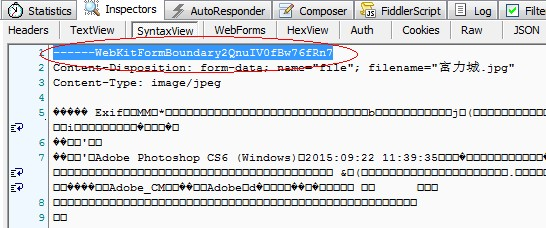
\includegraphics[scale=0.8]{HTTPPostSplitWithRawData.jpg}
	\caption{multipart/form-data请求的内容分割符标记图片流数据}
	\label{fig:HTTPPostSplitWithRawData}
\end{figure}

上传图片时会提示超过了最大请求长度,
原因是由于asp.net默认最大上传文件大小为4M,运行超时时间为90s。
在Web.config中添加如下配置可以改变这个默认值。

\begin{lstlisting}[language=HTML]
<system.web>
	<httpRuntime maxRequestLength="4096" executionTimeout="3600" />
</system.web>
\end{lstlisting}

前端的页面监测用户的拖放操作,并利用HTML5的FormData进行文件的提交。

\begin{lstlisting}[language=VBScript]
if (tests.dnd) {
    holder.ondragover = function () { this.className = "hover"; return false; };
    holder.ondragend = function () { this.className = ""; return false; };
    holder.ondrop = function (e) {
        this.className = "";
        e.preventDefault();
        readfiles(e.dataTransfer.files);
    }
} else {
    fileupload.className = "hidden";
    fileupload.querySelector('input').onchange = function () {
        readfiles(this.files);
    };
}
\end{lstlisting}

XMLHttpRequest Level 2添加了一个新的接口——FormData。
利用FormData对象,我们可以通过JavaScript用一些键值对来模拟一系列表单控件,
我们还可以使用XMLHttpRequest的send()方法来异步的提交表单。
与普通的Ajax相比,使用FormData的最大优点就是我们可以异步上传二进制文件。

\section{Cookie}

大多数浏览器支持最大为4096字节的Cookie。由于这限制了Cookie的大小,
最好用Cookie来存储少量数据,或者存储用户ID之类的标识符。用户ID随后便可用于标识用户,
以及从数据库或其他数据源中读取用户信息。浏览器还限制站点可以在用户计算机上存储的Cookie的数量。
大多数浏览器只允许每个站点存储20个Cookie;如果试图存储更多Cookie,
则最旧的Cookie便会被丢弃。有些浏览器还会对它们将接受的来自所有站点的Cookie总数作出绝对限制,通常为300个。
通过前面的内容,我们了解到Cookie是用于维持服务端会话状态的,通常由服务端写入,
在后续请求中,供服务端读取。下面本文将按这个过程看看Cookie是如何从服务端写入,
最后如何传到服务端以及如何读取的。 

\paragraph{会话Cookie(Session Cookie)}

不设置过期时间,则表示这个Cookie生命周期为浏览器会话期间,只要关闭浏览器窗口,Cookie就消失了。
生命期为浏览器会话期。一般不保存在硬盘上而是保存在内存里。

\paragraph{持久性Cookie(Persistent Cookie)}

设置了过期时间,浏览器就会把Cookie保存到硬盘上,关闭后再次打开浏览器,
这些Cookie依然有效直到超过设定的过期时间。
保存在用户硬盘上面,同一浏览器可以获取。

HTTP协议是无状态的,同一个客户端的这次请求和上次请求是没有对应关系,
对HTTP服务器来说,它并不知道这两个请求来自同一个客户端。 
为了解决这个问题, Web程序引入了Cookie机制来维护状态。
Cookie是由服务器端生成,发送给User-Agent(一般是浏览器),
浏览器会将Cookie的key/value保存到某个目录下的文本文件内,
下次请求同一网站时就发送该Cookie给服务器(前提是浏览器设置为启用Cookie)。
Cookie是可以被Web服务器设置的字符串,并且可以保存在浏览器中。
如图\ref{fig:CookieKeepStatus}所示,当浏览器访问了页面1时,web服务器设置了一个Cookie,
并将这个Cookie和页面1一起返回给浏览器,浏览器接到Cookie之后,就会保存起来,
在它访问页面2的时候会把这个Cookie也带上,Web服务器接到请求时也能读出Cookie的值,
根据Cookie值的内容就可以判断和恢复一些用户的信息状态。

\begin{figure}[htbp]
	\centering
	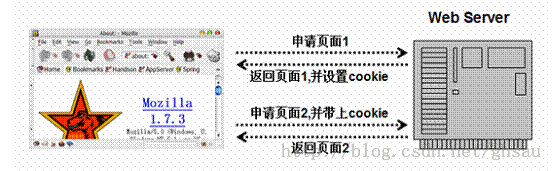
\includegraphics[scale=0.8]{CookieKeepStatus.jpg}
	\caption{Cookie HTTP保持状态}
	\label{fig:CookieKeepStatus}
\end{figure}

在Google Chrome的Cookie存储路径为:

\begin{lstlisting}
C:\Documents and Settings\Administrator\Local Settings\Application Data\Google\Chrome\User Data
\end{lstlisting}

Mozila Firefox的存储路径为:

\begin{lstlisting}
C:\Documents and Settings\Administrator\AppData\Local\Mozilla\Firefox\Profiles\d4l4tvw6.default\OfflineCache
\end{lstlisting}

Google Chrome和Firefox的Cookie存放在sqlite数据库中,
也可以使用sqlite数据库工具直接打开文件进行查看,
不过由于密码是BLOB格式存储的,不能看到明文密码,
Cookie名称和值可以由服务器端开发自己定义,
对于JSP而言也可以直接写入jsessionid,
这样服务器可以知道该用户是否合法用户以及是否需要重新登录等,
服务器可以设置或读取Cookies中包含信息,
借此维护用户跟服务器会话中的状态。
Cookies最典型的应用是判定注册用户是否已经登录网站,
用户可能会得到提示,是否在下一次进入此网站时保留用户信息以便简化登录手续,
这些都是Cookies的功用。另一个重要应用场合是“购物车”之类处理。
用户可能会在一段时间内在同一家网站的不同页面中选择不同的商品,
这些信息都会写入Cookies,以便在最后付款时提取信息。
通过上面这个例子,可以看到Cookie是很重要的,
识别是否是登陆用户,就是通过Cookie。  
假如截获了别人的Cookie是否可以冒充他人的身份登陆呢?  
当然可以, 这就是一种黑客技术叫Cookie欺骗。
利用Cookie欺骗, 不需要知道用户名密码。就可以直接登录,使用别人的账户做事。
有两种方法可以截获他人的Cookie:

1.通过XSS\footnote{为不和层叠样式表(Cascading Style Sheets,
CSS)的缩写混淆,故将跨站脚本攻击缩写为XSS}脚本攻击即跨站脚本攻击(Cross Site Scripting),
获取他人的Cookie. 

2.想办法获取别人电脑上保存的Cookie文件(这个比较难)。

\subsection{编辑Cookie}

在Google Chrome中编辑Cookie需要安装Edit This Cookie插件(或者另一款Cookies插件由http://www.hotcleaner.com/提供),
在FireFox中可通过Firebug编辑Cookie,
或者添加Cookie,如图\ref{fig:EditCookieUsingFireDebug}所示。

\begin{figure}[htbp]
	\centering
	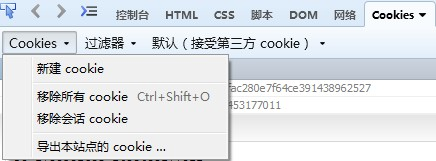
\includegraphics[scale=0.8]{EditCookieUsingFireFox.jpg}
	\caption{采用FireDebug编辑Cookie}
	\label{fig:EditCookieUsingFireDebug}
\end{figure}

需要注意Cookie的有效时间,
如果有效时间小于等于当前时间时需要调整有效时间,
否则添加的Cookie会因为时间超出而立即失效,
在编辑Cookie指定域的时候最好指定网址,
而不是IP地址+端口的形式,因为Cookie在端口支持方面至今未有标准,
Cookie可以说是不分端口(Cookies do not provide isolation by port),
Cookie跟站点(域名)对应,
例如同一个主机端口8889保存的Cookie在其他的端口同样能够读取\footnote{http://stackoverflow.com/questions/1612177/are-http-cookies-port-specific}。

\begin{quotation}
For historical reasons, cookies contain a number of security and privacy infelicities. 
For example, a server can indicate that a given cookie is intended for "secure" connections, 
but the Secure attribute does not provide integrity in the presence of an active network attacker. Similarly, cookies for a given host are shared across all the ports on that host, 
even though the usual "same-origin policy" used by web browsers isolates content retrieved via different ports.

\textbf{Cookies do not provide isolation by port.} If a cookie is readable by a service running 
on one port, the cookie is also readable by a service running on another port of the same server. If a cookie is writable by a service on one port, the cookie is also writable by a service 
running on another port of the same server. For this reason, 
servers SHOULD NOT both run mutually distrusting services on different ports of 
the same host and use cookies to store security sensitive information.
\end{quotation}


\section{Session}

Session又称为会话状态,是Web系统中最常用的状态,用于维护和当前浏览器实例相关的一些信息。
举个例子来说,我们可以把已登录用户的用户名放在Session中,这样就能通过判断Session中的某个Key来判断用户是否登录,
如果登录的话用户名又是多少。Session对于每一个客户端(或者说浏览器实例)是“人手一份”,
用户首次与Web服务器建 立连接的时候,服务器会给用户分发一个 SessionID作为标识。
SessionID是一个由24个字符组成的随机字符串。用户每次提交页面,
浏览器都会把这个SessionID包含在 HTTP头中提交给Web服务器,这样Web服务器就能区分当前请求页面的是哪一个客户端。
Session存储在服务器端,一般为了防止在服务器的内存中(为了高速存取),Sessinon在用户访问第一次访问服务器时创建,
需要注意只有访问JSP、Servlet等程序时才会创建Session,只访问HTML、IMAGE等静态资源并不会创建Session,
可调用request.getSession(true)强制生成Session。
服务器会把长时间没有活动的Session从服务器内存中清除,此时Session便失效。
Tomcat中Session的默认失效时间为20分钟。
虽然Session保存在服务器,对客户端是透明的,它的正常运行仍然需要客户端浏览器的支持。
这是因为Session需要使用Cookie作为识别标志。HTTP协议是无状态的,Session不能依据HTTP连接来判断是否为同一客户,
因此服务器向客户端浏览器发送一个名为JSESSIONID的Cookie,
它的值为该Session的id(也就是HttpSession.getId()的返回值)。Session依据该Cookie来识别是否为同一用户。





Session机制是一种服务器端的机制,服务器使用一种类似于散列表的结构(也可能就是使用散列表)来保存信息。
当程序需要为某个客户端的请求创建一个Session的时候,
服务器首先检查这个客户端的请求里是否已包含了一个session标识 - 称为session id,
如果已包含一个session id则说明以前已经为此客户端创建过Session,
服务器就按照session id把这个Session检索出来使用(如果检索不到,可能会新建一个),
如果客户端请求不包含session id,则为此客户端创建一个Session并且生成一个与此Session相关联的session id,
session id的值应该是一个既不会重复,又不容易被找到规律以仿造的字符串,
这个session id将被在本次响应中返回给客户端保存。 
保存这个session id的方式可以采用Cookie,这样在交互过程中浏览器可以自动的按照规则把这个标识发送给服务器。
一般这个Cookie的名字都是类似于SEEESIONID,而。比如WebLogic对于Web应用程序生成的Cookie:

\begin{lstlisting}
JSESSIONID=ByOK3vjFD75aPnrF7C2HmdnV6QZcEbzWoWiBYEnLerjQ99zWpBng!-145788764 
\end{lstlisting}

它的名字就是JSESSIONID,由于Cookie可以被人为的禁止,
必须有其他机制以便在Cookie被禁止时仍然能够把session id传递回服务器。
经常被使用的一种技术叫做URL重写,就是把session id直接附加在URL路径的后面,附加方式也有两种,
一种是作为URL路径的附加信息,表现形式为

\begin{lstlisting}
http://...../xxx;jsessionid=ByOK3vjFD75aPnrF7C2HmdnV6QZcEbzWoWiBYEnLerjQ99zWpBng!-145788764
\end{lstlisting}
 

另一种是作为查询字符串附加在URL后面,表现形式为

\begin{lstlisting}
http://...../xxx?jsessionid=ByOK3vjFD75aPnrF7C2HmdnV6QZcEbzWoWiBYEnLerjQ99zWpBng!-145788764 
\end{lstlisting}

这两种方式对于用户来说是没有区别的,只是服务器在解析的时候处理的方式不同,
采用第一种方式也有利于把session id的信息和正常程序参数区分开来。 
为了在整个交互过程中始终保持状态,就必须在每个客户端可能请求的路径后面都包含这个session id。

\subsection{Session的优点与限制}

Session的优点是它可以自动的进行页面间的参数传递。
不需要表单传递、不需要超链接传递,只需要在后台传递。
而且设了一次session之后,就可以在每一个页面使用,真的非常方便。
如果网站很大,一不小心设了两个同名的session,就会造成错误,
尤其是象session(“id”)这类变量,很容易出错。session会占用系统资源,
而且在20分钟内没有连接的情况下才会自动消失。所以一旦大量使用,将会对系统造成严重影响。

\subsection{Session的生命周期}

Session是在用户第一次访问网站 的时候创建的,那么Session是什么时候销毁的呢?
Session使用一种平滑超时的技术来控制何时销毁Session。默认情况下,
Session 的超时时间(Timeout)是20分钟,用户保持连续20分钟不访问网站,
则Session被收回,如果在这20分钟内用户又访问了一次页面,那么20 分钟就重新计时了,
也就是说,这个超时是连续不访问的超时时间,而不是第一次访问后20分钟必过时。
这个超时时间同样也可以通过调整Web.config文件进行修改。
别太相信Session的Timeout属性,如果你把它设置为24小时,
则很难相信24小时之后用户的Session还在。Session是否 存在,不仅仅依赖于Timeout属性,
以下的情况都可能引起Session丢失(所谓丢失就是在超时以前原来的Session无效)。

\begin{itemize}
\item{\textbf{bin目录中的文件被改写}}~~asp.net有一种机制,为了保证dll重新编译之后,系统正常运行,它会重新启动一次网站进程,这时就会导致Session丢失,所以如果有access数据库位于bin目录,或者有其他文件被系统改写,包括创建新文件、修改文件名、修改文件内容、删除文件、修改目录名、删除目录就会导致Session丢失,新建目录IIS不会重启。
\item{\textbf{SessionID丢失或者无效}}~~如果你在URL中存储SessionID,但是使用了绝对地址重定向网站导致URL中的SessionID丢失,那么原 来的Session将失效。如果你在Cookie中存储SessionID,那么客户端禁用Cookie或者Cookie达到了IE中Cookie数量的 限制(每个域20个),那么Session将无效。
\item{\textbf{如果使用InProc的Session,那么IIS重启将会丢失Session}}~~同理,如果使用StateServer的Session,服务器重新启动Session也会丢失。
\item{\textbf{进程用户名更改权限后}}~~例如Network Service更改权限后也会导致IIS重新启动,Session会丢失。
\end{itemize}

一般来说,如果在IIS中存储Session而且Session的Timeout设置得比较长,
再加上Session中存储大量的数据,非常容易发生Session丢失的问题。
最后, Session的安全性怎么样呢?我们知道,Session中只有SessionID是存储在客户端的,
并且在页面每次提交的过程中加入HTTP头发送给 服务器。SessionID只是一个识别符,
没有任何内容,真正的内容是存储在服务器上的。总的来说安全性还是可以的,
不过笔者建议你不要使用 cookieless和SqlServer模式的Session。把SessionID暴露在URL中,
把内容存储在数据库中可能会发生攻击隐患。

\subsection{网页嵌入视频}

网页嵌入视频代码如下:

\begin{lstlisting}[language=HTML]
<div>
  <center style="margin-bottom:20px">
    <embed src="http://player.youku.com/player.php/sid/XNzA1ODUyNjYw/v.swf" allowfullscreen="true"
           quality="high" 
           width="480" 
           height="400" 
           align="middle" 
           allowscriptaccess="always" 
           type="application/x-shockwave-flash" />
    </center>        
</div>
\end{lstlisting}

例如网页中嵌入FSF的介绍视频: 

\begin{lstlisting}[language=HTML]
<video src="//static.fsf.org/nosvn/FSF30-video/FSF_30_720p.webm" controls width="640" height="390"></video>
\end{lstlisting}

\section{缓存(Cache)}

网页缓存由 HTTP消息头中的Cache-control控制,
常见取值有private、no-cache、max-age、must- revalidate等,默认为private。
浏览器会自动缓存网页的css,js等文件,
有时为了强制浏览器进行缓存刷新,
可修改css文件的链接,
例如添加版本号等等。
如更新了服务器上的example.css文件,
希望浏览器立即使用新的样式,可将链接改成如下形式。

\begin{lstlisting}[language=HTML]
<link rel="stylesheet" type="text/css" href="http://static.zouwo.com/lottery/1.02/css/lottery2.css?v=1.0.1" />
\end{lstlisting}

其中?v=1.0.1是新加入的内容,此时css链接与本地不一致,
浏览器会下载新的css样式表。
根据标准,到目前为止,HTML5一共有6种缓存机制,有些是之前已有,有些是HTML5才新加入的。

\begin{itemize}
\item{浏览器缓存机制}
\item{Dom Storage(Web Storage)存储机制}
\end{itemize}

浏览器缓存机制是指通过HTTP协议头里的Cache-Control(或 Expires)和Last-Modified(或 Etag)等字段来控制文件缓存的机制。这两个字段配置的是本地缓存,
如果缓存命中(当前时间小于资源的过期时间)那么浏览器是不会发起HTTP请求而是直接加载缓存资源。
这(Expires)是WEB中较早的缓存机制,是在HTTP 1.0协议中实现的,
它描述的是一个绝对时间,由服务器返回,用GMT格式的字符串表示。
有点不同于Dom Storage、AppCache 等缓存机制,
但本质上是一样的。可以理解为,一个是协议层实现的,一个是应用层实现的。

\subsection{Request缓存相关首部字段}

\paragraph{Cache-Control}Expires和Cache-Control同时存在时,
Cache-Control优先级高于Expires,
Cache-Control在HTTP 1.1中加入的,
用于控制文件在本地缓存有效时长。最常见的,比如服务器回包:
Cache-Control:max-age=600表示文件在本地应该缓存,
且有效时长是600秒(从发出请求算起)。在接下来600秒内,如果有请求这个资源,
浏览器不会发出HTTP请求,而是直接使用本地缓存的文件。
许多人以为,出于安全考虑,浏览器不会在本地保存HTTPS缓存。实际上,只要在HTTP头中使用特定命令,HTTPS是可以缓存的。
Firefox默认只在内存中缓存HTTPS。但是,只要头命令中有Cache-Control: Public,缓存就会被写到硬盘上。
只要HTTP头允许这样做,所有版本的IE都缓存HTTPS内容。比如,如果头命令是Cache-Control: max-age=600,那么这个网页就将被IE缓存10分钟。IE的缓存策略,与是否使用HTTPS协议无关。
(其他浏览器在这方面的行为不一致,取决于你使用的版本)

\begin{itemize}
\item{no-cache}~~不直接使用缓存,始终向服务器发起请求。表示必须先与服务器确认返回的响应是否被更改,然后才能使用该响应来满足后续对同一个网址的请求。因此,如果存在合适的验证令牌 (ETag),no-cache会发起往返通信来验证缓存的响应,如果资源未被更改,可以避免下载。
\item{no-store}~~禁止缓存任何响应,也就是说每次用户请求资源时,都会向服务器发送一个请求,每次都会下载完整的响应。
\item{max-age}~~缓存过期时间,是一个时间数值,比如3600秒,设置为0的时候效果等同于no-cache
\item{private(default)}~~浏览器可以缓存private响应,但是通常只为单个用户缓存,因此,不允许任何代理服务器对其进行缓存 。比如,用户浏览器可以缓存包含用户私人信息的HTML网页,但是CDN不能缓存。
\item{s-maxage}~~给缓存代理用的指令,对直接返回资源的server无效,当s-maxage生效时,会忽略max-age的值
\item{only-if-cached}~~若有缓存,则只使用缓存,若缓存文件出问题了,请求也会出问题
\end{itemize}

\paragraph{Last-Modified}是标识文件在服务器上的最新更新时间。下次请求时,如果文件缓存过期,
浏览器通过If-Modified-Since字段带上这个时间,发送给服务器,由服务器比较时间戳来判断文件是否有修改。
如果没有修改,服务器返回304告诉浏览器继续使用缓存;如果有修改,则返回200,同时返回最新的文件。
Cache-Control通常与 Last-Modified一起使用。一个用于控制缓存有效时间,一个在缓存失效后,
向服务查询是否有更新。Cache-Control还有一个同功能的字段:Expires。
Expires 的值一个绝对的时间点,如:Expires: Thu, 10 Nov 2015 08:45:11 GMT,
表示在这个时间点之前,缓存都是有效的。
Expires是HTTP1.0标准中的字段,Cache-Control是HTTP1.1标准中新加的字段,
功能一样,都是控制缓存的有效时间。当这两个字段同时出现时,Cache-Control 是高优化级的。
分布式系统里多台机器间文件的Last-Modified必须保持一致,以免负载均衡到不同机器导致比对失败。

\paragraph{Etag(Entity Tag)}Etag也是和Last-Modified 一样,对文件进行标识的字段。不同的是,Etag的取值是一个对文件进行标识的特征字串。
在向服务器查询文件是否有更新时,浏览器通过If-None-Match字段把特征字串发送给服务器,
由服务器和文件最新特征字串进行匹配,
来判断文件是否有更新。没有更新回包304,有更新回包200。
Etag和Last-Modified可根据需求使用一个或两个同时使用。
两个同时使用时,只要满足其中一个条件,就认为文件没有更新。Last-Modified需要向服务器发起查询请求,
才能知道资源文件有没有更新。虽然服务器可能返回304告诉没有更新,但也还有一个请求的过程。
对于移动网络,这个请求可能是比较耗时的。有一种说法叫“消灭304”,指的就是优化掉304的请求。
抓包发现,带 if-Modified-Since 字段的请求,如果服务器回包304,
回包带有Cache-Control:max-age或Expires 字段,
文件的缓存有效时间会更新,就是文件的缓存会重新有效。304回包后如果再请求,则又直接使用缓存文件了,
不再向服务器查询文件是否更新了,除非新的缓存时间再次过期。
分布式系统尽量关闭掉ETag(每台机器生成的ETag都会不一样)。

另外,Cache-Control与Last-Modified是浏览器内核的机制,一般都是标准的实现,不能更改或设置。
以QQ浏览器的X5为例,Cache-Control与Last-Modified 缓存不能禁用。
缓存容量是12MB,不分HOST,过期的缓存会最先被清除。如果都没过期,应该优先清最早的缓存或最快到期的或文件大小最大的;
过期缓存也有可能还是有效的,清除缓存会导致资源文件的重新拉取。

还有,浏览器,如 X5,在使用缓存文件时,是没有对缓存文件内容进行校验的,这样缓存文件内容被修改的可能。

分析发现,浏览器的缓存机制还不是非常完美的缓存机制。完美的缓存机制应该是这样的:

\begin{enumerate}
\setcounter{enumi}{0}
\item{缓存文件没更新,尽可能使用缓存,不用和服务器交互}
\item{缓存文件有更新时,第一时间能使用到新的文件}
\item{缓存的文件要保持完整性,不使用被修改过的缓存文件}
\item{缓存的容量大小要能设置或控制,缓存文件不能因为存储空间限制或过期被清除}
\end{enumerate}

以X5为例,第1、2条不能同时满足,第3、4条都不能满足。
在实际应用中,为了解决 Cache-Control 缓存时长不好设置的问题,以及为了”消灭304“,Web前端采用的方式是:
在要缓存的资源文件名中加上版本号或文件 MD5值字串,如 common.d5d02a02.js,common.v1.js,
同时设置 Cache-Control:max-age=31536000,也就是一年。在一年时间内,资源文件如果本地有缓存,
就会使用缓存;也就不会有304的回包。如果资源文件有修改,则更新文件内容,同时修改资源文件名,
如 common.v2.js,html页面也会引用新的资源文件名。通过这种方式,实现了:缓存文件没有更新,则使用缓存;
缓存文件有更新,则第一时间使用最新文件的目的。即上面说的第1、2条。第3、4条由于浏览器内部机制,目前还无法满足。
因为Cache-Control与Expires的作用一致,Last-Modified与ETag的作用也相近。但它们有以下区别,
如图\ref{fig:HttpCacheControlEtag}所示:

\begin{figure}[!b]
	\centering
	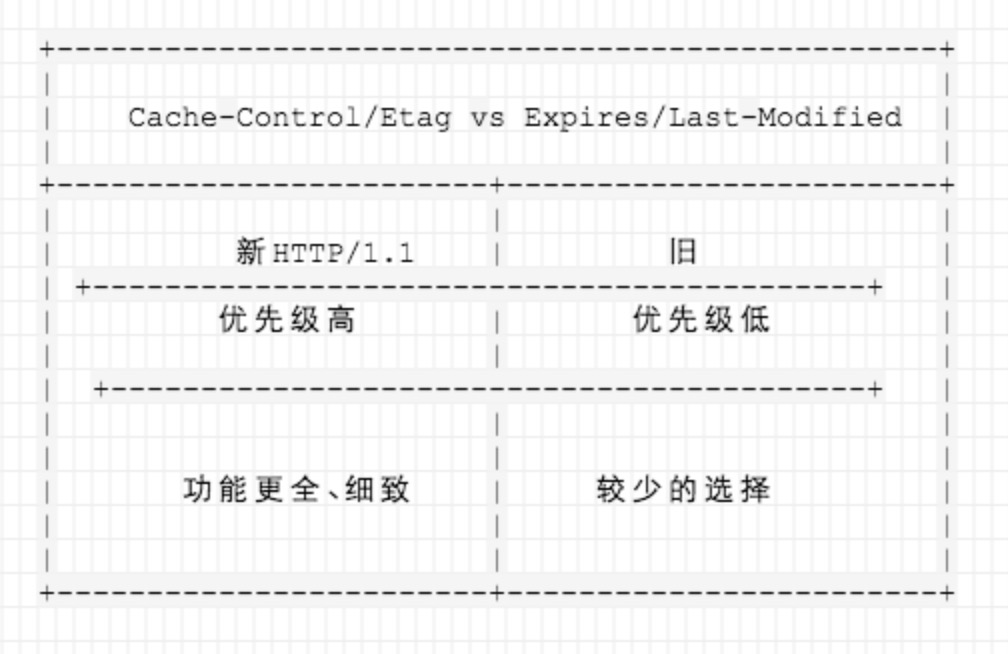
\includegraphics[scale=1]{HttpCacheControlEtag.jpg}
	\caption{HTTP Cache-Control和Etag区别}
	\label{fig:HttpCacheControlEtag}
\end{figure}

现在默认浏览器均默认使用HTTP 1.1,所以Expires和Last-Modified的作用基本可以忽略,
具备Cache-Control和Etag即可。

\paragraph{Pragma}用来做缓存过期判断,它可以取值no-cache,
这是一个http1.0遗留的字段,当它和Cache-Control同时存在的时候,会被Cache-Control覆盖

\paragraph{if-match/if-none-match}用来做资源更新判断,
这个指令会把缓存中的Etag传给服务器,服务器用它来和服务器端的资源Etag进行对比,
若不一致则证明资源被修改了,需要响应请求为 200 OK

\paragraph{if-modified-since}用来做资源更新判断,
这个指令会把文件的上一次缓存中的文件的更新时间传给服务器,
服务器判断文件在这个时间点后是否被修改,如果被修改过则需要响应请求为200 OK

\subsection{Response缓存相关首部字段}

\subsection{System.Web.Caching}

System.Web.Caching命名空间提供用于缓存服务器上常用数据的类。
这包括Cache类,该类是一个使您可以存储任意数据对象(如哈希表和数据集)的词典。
它还为这些对象提供到期功能,并提供使您可以添加和移除对象的方法。
您还可以添加依赖于其他文件或缓存项的对象,
并在从Cache中移除对象时执行回调以通知应用程序。
将页面与Controller和Action对应的数据存储在XML配置文件中。

\section{浏览器渲染(Browser Render)}

Javascript的使用一定要在Javascript的引用之后,
否则会出现未定义(undefined)错误,
例如页面中的JavaScript脚本使用了如下语句:

\begin{lstlisting}[language=VBScript]
config.backUrl="http://www.baidu.com"
\end{lstlisting}

但是config对象在另一个JavaScript脚本中,
那么引用脚本一定要在加载脚本之前。
<script> 标签引入脚本有三种情况:

\subparagraph{立即执行}

<script src="a.js"><script src="b.js">顺序:保证先后顺序。
解析:HTML 解析器遇到它们时,将阻塞(停止解析标签后的文档),待脚本下载完成并执行后,继续解析标签之后的文档。

\subparagraph{推迟执行}

<script defer src="a.js">
<script defer src="b.js">顺序:保证先后顺序。
解析:HTML 解析器遇到它们时,不阻塞(脚本将被异步下载),待文档解析完成之后,执行脚本。

\subparagraph{尽快执行}

<script async src="a.js"><script async src="b.js">顺序:不保证先后顺序。
解析:HTML 解析器遇到它们时,不阻塞(脚本将被异步下载,一旦下载完成,立即执行它),并继续解析之后的文档。

HTML页面加载和解析流程:

\begin{itemize}
\item{用户输入网址(假设是个html页面,并且是第一次访问),浏览器向服务器发出请求,服务器返回html文件}
\item{浏览器开始载入html代码,发现<head>标签内有一个<link>标签引用外部CSS文件}
\item{浏览器又发出CSS文件的请求,服务器返回这个CSS文件}
\item{浏览器继续载入html中<body>部分的代码,并且CSS文件已经拿到手了,可以开始渲染页面了}
\item{浏览器在代码中发现一个<img>标签引用了一张图片,向服务器发出请求。此时浏览器不会等到图片下载完,而是继续渲染后面的代码}
\item{服务器返回图片文件,由于图片占用了一定面积,影响了后面段落的排布,因此浏览器需要回过头来重新渲染这部分代码}
\item{浏览器发现了一个包含一行Javascript代码的<script>标签,赶快运行它}
\item{Javascript脚本执行了这条语句,它命令浏览器隐藏掉代码中的某个<style>(style.display=”none”)。杯具啊,突然就少了这么一个元素,浏览器不得不重新渲染这部分代码}
\end{itemize}

9. 终于等到了</html>的到来,浏览器泪流满面……
10. 等等,还没完,用户点了一下界面中的“换肤”按钮,Javascript让浏览器换了一下<link>标签的CSS路径。
11. 浏览器召集了在座的各位<div><span><ul><li>们,“大伙儿收拾收拾行李,咱得重新来过……”,浏览器向服务器请求了新的CSS文件,重新渲染页面。

reflow几乎是无法避免的。现在界面上流行的一些效果,比如树状目录的折叠、展开(实质上是元素的显示与隐藏)等,
都将引起浏览器的 reflow。鼠标滑过、点击……只要这些行为引起了页面上某些元素的占位面积、定位方式、边距等属性的变化,
都会引起它内部、周围甚至整个页面的重新渲染。reflow问题是可以优化的,我们可以尽量减少不必要的reflow。
例子中的<img>图片载入问题,这其实就是一个可以避免的reflow——给图片设置宽度和高度就可以了。
这样浏览器就知道了图片的占位面积,在载入图片前就预留好了位置。
另外,有个和reflow看上去差不多的术语:repaint,中文叫重绘。
如果只是改变某个元素的背景色、文字颜色、边框颜色等等不影响它周围或内部布局的属性,
将只会引起浏览器repaint。repaint的速度明显快于reflow(在IE下需要换一下说法,reflow要比repaint 更缓慢)。

\begin{figure}[htbp]
	\centering
	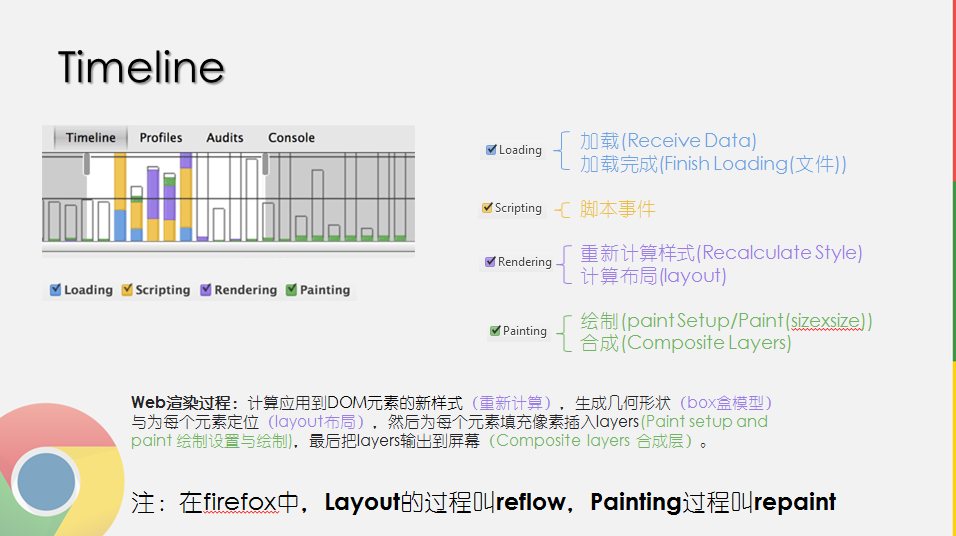
\includegraphics[scale=0.5]{ChromeRenderingTimeLine.png}
	\caption{浏览器渲染TimeLine}
	\label{fig:ChromeRenderingTimeLine}
\end{figure}

\subsection{重绘(Redraw)与重排(Reflow)}

浏览器从下载文档到显示页面的过程是个复杂的过程,这里包含了重绘和重排。
各家浏览器引擎的工作原理略有差别,但也有一定规则。简单讲,通常在文档初次加载时,
浏览器引擎会解析HTML文档来构建DOM树,之后根据DOM元素的几何属性构建一棵用于渲染的树。
渲染树的每个节点都有大小和边距等属性,
类似于盒子模型(由于隐藏元素不需要显示,渲染树中并不包含DOM树中隐藏的元素)。
当渲染树构建完成后,浏览器就可以将元素放置到正确的位置了,再根据渲染树节点的样式属性绘制出页面。
由于浏览器的流布局,对渲染树的计算通常只需要遍历一次就可以完成。但table及其内部元素除外,
它可能需要多次计算才能确定好其在渲染树中节点的属性,通常要花3倍于同等元素的时间。
这也是为什么我们要避免使用table做布局的一个原因。

\textbf{重绘(Redraw)}是一个元素外观的改变所触发的浏览器行为,例如改变visibility、outline、背景色等属性。
浏览器会根据元素的新属性重新绘制,使元素呈现新的外观。重绘不会带来重新布局,并不一定伴随重排。
\textbf{重排(Redraw)}是更明显的一种改变,可以理解为渲染树需要重新计算。下面是常见的触发重排的操作:

1. DOM元素的几何属性变化

当DOM元素的几何属性变化时,渲染树中的相关节点就会失效,浏览器会根据DOM元素的变化重新构建渲染树中失效的节点。
之后,会根据新的渲染树重新绘制这部分页面。而且,当前元素的重排也许会带来相关元素的重排。
例如,容器节点的渲染树改变时,会触发子节点的重新计算,也会触发其后续兄弟节点的重排,
祖先节点需要重新计算子节点的尺寸也会产生重排。最后,每个元素都将发生重绘。可见,
重排一定会引起浏览器的重绘,一个元素的重排通常会带来一系列的反应,甚至触发整个文档的重排和重绘,性能代价是高昂的。

2. DOM树的结构变化

当DOM树的结构变化时,例如节点的增减、移动等,也会触发重排。浏览器引擎布局的过程,
类似于树的前序遍历,是一个从上到下从左到右的过程。通常在这个过程中,当前元素不会再影响其前面已经遍历过的元素。
所以,如果在body最前面插入一个元素,会导致整个文档的重新渲染,而在其后插入一个元素,则不会影响到前面的元素。

3. 获取某些属性

浏览器引擎可能会针对重排做了优化。比如Opera,它会等到有足够数量的变化发生,或者等到一定的时间,或者等一个线程结束,
再一起处理,这样就只发生一次重排。但除了渲染树的直接变化,当获取一些属性时,浏览器为取得正确的值也会触发重排。
这样就使得浏览器的优化失效了。这些属性包括:offsetTop、offsetLeft、 offsetWidth、
offsetHeight、scrollTop、scrollLeft、scrollWidth、scrollHeight、clientTop、cli
entLeft、clientWidth、clientHeight、getComputedStyle() (currentStyle in IE)。
所以,在多次使用这些值时应进行缓存。此外,改变元素的一些样式,调整浏览器窗口大小等等也都将触发重排。
开发中,比较好的实践是尽量减少重排次数和缩小重排的影响范围。例如:

\begin{itemize}
\item{将多次改变样式属性的操作合并成一次操作。}
\item{将需要多次重排的元素,position属性设为absolute或fixed,这样此元素就脱离了文档流,它的变化不会影响到其他元素。例如有动画效果的元素就最好设置为绝对定位。}
\item{在内存中多次操作节点,完成后再添加到文档中去。例如要异步获取表格数据,渲染到页面。可以先取得数据后在内存中构建整个表格的html片段,再一次性添加到文档中去,而不是循环添加每一行。}
\item{由于display属性为none的元素不在渲染树中,对隐藏的元素操作不会引发其他元素的重排。如果要对一个元素进行复杂的操作时,可以先隐藏它,操作完成后再显示。这样只在隐藏和显示时触发2次重排。}
\item{在需要经常获取那些引起浏览器重排的属性值时,要缓存到变量。}
\end{itemize}

\section{网页跳转(Page Redirect)}

在JavaScript中的写法,
虽然window.location和window.location.href都可以达到跳转的效果,
但是建议使用window.location.href,
具体原因参考以下注解\footnote{注解的来源:http://stackoverflow.com/questions/2383401/javascript-setting-location-href-versus-location}。

\begin{lstlisting}[language=VBScript]
window.location = "http://www.baidu.com";
window.location.href = "http://www.baidu.com";`\makeremark{Like as has been said already, location is an object. But that person suggested using either. But, you will do better to use the .href version.Objects have default properties which, if nothing else is specified, they are assumed. In the case of the location object, it has a property called .href. And by not specifying ANY property during the assignment, it will assume "href" by default.This is all well and fine until a later object model version changes and there either is no longer a default property, or the default property is changed. Then your program breaks unexpectedly.}`
\end{lstlisting}

\showremarks

window.location对象用于获得当前页面的地址(URL),
并把浏览器重定向到新的页面。
window.location对象在编写时可不使用window这个前缀。
location.href属性返回当前页面的URL。

\subsection{Redirect}

网页重定向在.NET中的写法如下代码片段所示(属于服务器端重定向)。

\begin{lstlisting}[language={[Sharp]C}]
System.Web.HttpContext.Current.Response.Redirect("http://www.baidu.com", true);
\end{lstlisting}

第一个参数为需要重定向到的网络链接,
第二个参数为是否结束此次会话(endResponse),默认为true。
Redirect在跳转时url如果写成Home/Index,那么将在当前链接后附加Home/Index路径。
例如当前链接为:http://192.168.1.1/Detail,
那么重定向后的路径为

\begin{lstlisting}[language=HTML]
http://192.168.1.1/Detail/Home/Index
\end{lstlisting}

如果写成/Home/Index(注意Home前面多一个斜杠),
那么跳转的链接为

\begin{lstlisting}[language=HTML]
http://192.168.1.1/Home/Index
\end{lstlisting}

在后台链接会自动跳转到指定的URL地址。
服务器端并没有返回请求页面的html数据,
而是Response了一个302 Found,
并在Location中给出了目标URL,
这就是在告诉浏览器:请重新发出一个HTTP请求,
所请求的URL为返回的URL。
浏览器于是按照吩咐,重新发出了一个http的请求。
这就是服务器Redirect重定向的过程。
当服务器执行到Response.Redirect语句时,
会立即中断页面的生命周期,直接向客户端返回信息,让客户端进行重定向操作。
从Redirect(重定向)的流程可以看出,Redirect比较耗时,
它仅用于用于从当前物理服务器开发跳转到其它服务器。
如果只是在本服务器开发内页面跳转请使用Server.Transfer语法,
这样会减少很多没有必要的客户端重定向。
如果网站指定是永久性转移则返回HTTP 301状态码,
如果是临时性转移,则返回HTTP 302状态码,
两者仅仅是状态码不相同而已,都是同样的实现原理,
从源码\ref{code:PageRedirect}(System.Web.dll)中可以看出。

\begin{lstlisting}[language={[Sharp]C},caption=Redirect实现片段,label={code:PageRedirect}]
this.StatusCode = permanent ? 301 : 302;
this.RedirectLocation = url;
url = !UriUtil.IsSafeScheme(url) ? HttpUtility.HtmlAttributeEncode(HttpUtility.UrlEncode(url)) : HttpUtility.HtmlAttributeEncode(url);
this.Write("<html><head><title>Object moved</title></head><body>\r\n");
this.Write("<h2>Object moved to <a href=\"" + url + "\">here</a>.</h2>\r\n");
this.Write("</body></html>\r\n");
\end{lstlisting}

\subsection{Meta Refresh}

跳转有时还需要在指定的时长后进行跳转,
可用Javascript的setInterval和setTimeOut方法。
有时前2种方式会失效,如在机顶盒内置浏览器中(应该是写法错误导致),
那么可以采用如下语句进行指定时间后的跳转。

\begin{lstlisting}[language=HTML]
<meta http-equiv="refresh" content="5;url=/ShaPingBa/Index" />
\end{lstlisting}

其中url为跳转的目标地址,5表示5秒后跳转。
注意这种方式在2000年前比较流行,通过网页中的meta指令,
在特定时间后重定向到新的网页,如果延迟的时间太短(约5秒之内),
会被搜索引擎判断为spam,遭到惩罚。
在MVC中还可以使用RedirectToAction进行网页的跳转,
此方法有多个重载。 

\subsection{Server.Transfer}

\begin{lstlisting}[language={[Sharp]C}]
Server.Transfer("WebForm2.aspx",True)
\end{lstlisting}

Server.Transfer方法的另一个参数——"preserveForm"。
如果你设置这个参数为True,那么querystring和任何form变量都会同时传递到你定位的页面。
如果要将执行流程转入同一Web服务器的另一个ASPX页面,
应当使用Server.Transfer而不是Response.Redirect,
因为Server.Transfer能够避免不必要的网络通信,从而获得更好的性能和浏览效果。
页面A跳转到页面B,同时页面处理的控制权也进行移交,
在跳转过程中Request,Session等保存的信息不变,
浏览器的URL仍保存A的URL信息.
Server.Transfer的重定向请求在服务器端进行,
客户端不知晓服务器执行了页面转换,因此URL保持不变,
Server.Transfer属于服务器端跳转。
Server.Transfer页面跳转的效率比Response.Redirect高;
且由于在服务器上执行,可以兼容任何浏览器,但是只能在IIS服务器下运行。
在MVC下的写法为:

\begin{lstlisting}[language={[Sharp]C}]
//使用TransferRequest效率更高,不需304回包,浏览器链接不变
HttpContext.Server.TransferRequest("~/Houses/IndexNew");
\end{lstlisting}

跳转后浏览器的Url不变,跳转后的页面可以使用跳转前的页面的参数。

\subsection{URL锚点(Fragment URLs)}

页面之所以能定位到锚点所在位置,
都是因为URL地址中的锚链的作用,
而不是点击行为。最好的证据就是,
当重新载入带有锚链的页面时,锚点依然会被定位。
\#代表网页中的一个位置。其右面的字符,就是该位置的标识符。
在第一个\#后面出现的任何字符,都会被浏览器解读为位置标识符。
这意味着,这些字符都不会被发送到服务器端\footnote{http://www.ruanyifeng.com/blog/2011/03/url\_hash.html}。

\section{技巧(Little Tricks)}

\subsection{查看Cookie登录密码}

在Firefox中可以查看所有网站Cookie保存的密码,
在Firefox选项-->安全里面,
如图\ref{fig:firefoxBrowserPassword}所示。

\begin{figure}[htbp]
	\centering
	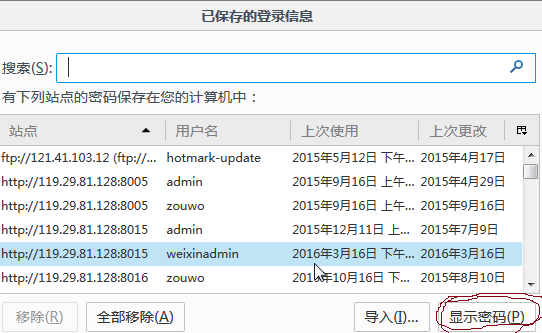
\includegraphics[scale=0.8]{firefoxBrowserPassword.png}
	\caption{在Firefox中查看网站的登录密码}
	\label{fig:firefoxBrowserPassword}
\end{figure}

\subsection{刷新当前页面(Refresh Current Page)}

微信开发过程中,由于微信浏览器Android下没有刷新按钮,
每次修改数据需要重新进入修改页面比较麻烦,
可在每个页面中添加一个刷新按钮,直接点击按钮刷新,
部署后将按钮注释即可,在MVC的布局页中添加刷新标签,
如代码\ref{code:refreshCurrentPageForDebug}所示。

\begin{lstlisting}[language=HTML,caption=添加刷新按钮便于调试,label={code:refreshCurrentPageForDebug}]
<body style="background-color:#f3f3f3;">
    <div class="s_part1"><a href="javascript:window.location.reload()">Refresh</a></div>
    @RenderBody()
</body>
\end{lstlisting}

也可以判断当前程序集是发布状态还是调试状态,
根据程序集状态来判断是否需要添加用于调试的刷新按钮。

\begin{lstlisting}[language={[Sharp]C},caption=获取程序集是否为调试状态]
#region Is Debug Model
/// <summary>
/// 
/// </summary>
/// <param name="dllPath">Assembly path</param>
/// <returns></returns>
public static bool IsDebugged(string dllPath)
{
    var assembly =Assembly.LoadFile(Path.GetFullPath(dllPath));
    return assembly.GetCustomAttributes(false).OfType<DebuggableAttribute>().Any(debuggableAttribute => debuggableAttribute.IsJITTrackingEnabled);
}
#endregion
\end{lstlisting}

dllPath为程序集的路径,获取程序集的路径如下代码所示。

\begin{lstlisting}[language={[Sharp]C},caption=获取程序集路径]
var applicationPath = Assembly.GetExecutingAssembly().Location;
var currentApplicationPath = GetType().Assembly.Location;
\end{lstlisting}

判断程序集是调试(Debug)选项编译还是发布(Release)选项编译也可以观察反编译程序集的Debuggable值,
用ILSpy分别打开不同编译选项的程序集,
可以看到调试编译和发布编译DebuggingModes值不同,如下片段所示。

\begin{lstlisting}[language=Bash,caption=查看程序集调试模式]
#打开Release模式编译的程序集
[assembly: Debuggable(DebuggableAttribute.DebuggingModes.IgnoreSymbolStoreSequencePoints)]
#打开Debug模式编译的程序集
[assembly: Debuggable(DebuggableAttribute.DebuggingModes.Default | DebuggableAttribute.DebuggingModes.DisableOptimizations | DebuggableAttribute.DebuggingModes.IgnoreSymbolStoreSequencePoints | DebuggableAttribute.DebuggingModes.EnableEditAndContinue)]
\end{lstlisting}

序列点是用于指示调试器用户将希望能够来指代唯一的 Microsoft 中间语言 (MSIL) 代码中的位置,
例如用于设置断点。JIT 编译器可确保它不会将在两个不同的序列点 MSIL 编译成单个的本机指令。
默认情况下,JIT 编译器将检查符号存储区的其他序列点列表的程序数据库 (PDB) 文件中。
但是,加载 PDB 文件要求该文件可用并且具有负面性能影响。从 2.0 版开始,
编译器可以发出"隐式序列点"在 MSIL 代码流通过使用 MSIL"nop" 说明进行操作。
此类编译器应设置 IgnoreSymbolStoreSequencePoints 标志来通知公共语言运行时不会加载 PDB 文件。

\subsubsection{VPN网络访问}

在使用重庆有线VPN服务器时,由于远程VPN服务器限制只能与特定的用于开发的服务器进行通信,
导致连接VPN的同时本机无法访问互联网。
在VPN的属性设置中勾选掉“在远程网路上使用默认网关”选项即可解决此问题,
如图\ref{fig:UsingInternetWhenConnectVPN}所示。

\begin{figure}[htbp]
	\centering
	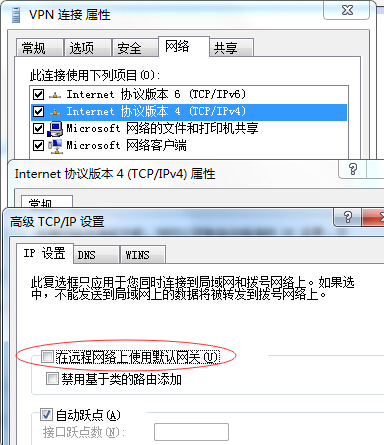
\includegraphics[scale=0.8]{UsingInternetWhenConnectVPN.jpg}
	\caption{VPN默认使用本机网关}
	\label{fig:UsingInternetWhenConnectVPN}
\end{figure}

\paragraph{勾选的优劣}好处: 无需添加静态路由即可访问 VPN 服务后面的局域网资源。
不足: VPN 拨上号后,本地无法上网,需要在 VPN 服务器上开通“到 Internet 的VPN路由通道” 才行。此外,即使开通了VPN路由通道,通过 VPN 上网速度可能会比较慢 (没有本地线路快)。
评点: 需要访问远程局域网时,进行 VPN 拨号,不需要时断开,但不适合“本地上网”和“访问远程局域网”同时进行的场合。

\paragraph{不勾选的优劣}

好处: 不改变本地默认网关,VPN 拨号后本地上网不受影响,仍然走本地线路。
不足: 访问远程局域网资源时,需要手动添加静态路由。
点评: 手动添加静态路由比较麻烦,可以通过批处理文件来辅助完成。
综合以上分析,得出以下结论:如果 VPN 客户端不需要访问远程局域网,只需要拨入客户端之间可以相互访问,则不用勾选 “默认网关”;如果需要,但是又不想手动添加静态路由,则可以采用第2种方案。

将VPN连接快捷方式拖动到启动项中,并将VPN连接属性-选项-“提示名称密码、和证书等”选项取消勾选,
可在开机时自动连接VPN,避免使用VPN时却发现VPN被占用导致无法连接VPN的尴尬,
宁愿占着茅坑不用,也不要内急时找不到茅坑,
Windows 7的启动文件夹为:

\begin{lstlisting}
C:\Users\Administrator\AppData\Roaming\Microsoft\Windows\Start Menu\Programs\Startup。
\end{lstlisting}

\subsection{URL特殊参数传递}

要把一个字符串作为URL参数传递给另一个页面,
必须要保证传递的字符串是正确的,能够被目标页面正确识别。
但由于URL传递时会造成某些冲突。
比如,你要传递的字符串也是一个带有参数的URL,
如需要传递的参数是如下形式的字符串:

\begin{lstlisting}
http://www.oyksoft.com/a.asp?b=1&c=2&d=3
\end{lstlisting}

要把这个URL字符串传递给http://www.oyksoft.com/e.asp,参数为url。
如果不作任何处理,那么就是这样:

\begin{lstlisting}
http://www.oyksoft.com/e.asp?url=http://www.oyksoft.com/a.asp?b=1&c=2&d=3
\end{lstlisting}

这样是很混乱的,它肯定会把c和d认为是传参,
而解析出的url参数为

\begin{lstlisting}[language=HTML]
http://www.oyksoft.com/a.asp?b=1
\end{lstlisting}

这样理解当然是错误的了,所以我们必须对原字符串进行重新编码。
在ASP和Javascript里面,有escape和unescape可以解决问题,
现在已不推荐使用。
注意escape方法不能够用来对统一资源标示码(URI)进行编码。
对其编码应使用encodeURI和encodeURIComponent方法。
例如调用另一个网页完成支付功能,
用户支付完毕后再回到指定的网页,
那么就需要将指定的网页编码后以参数的形式传递给支付页,
支付页再进行回调,编码并跳转到指定页如下代码片段所示。

\begin{lstlisting}[language=VBScript]
var callbackUrl = "http://www.oyksoft.com/a.asp?b=1&c=2&d=3";
var encodeCallbackUrl = encodeURIComponent(callbackUrl);
var payUrl = "http://www.oyksoft.com/a.asp?url=" + encodeCallbackUrl;
window.location.href = payUrl;
\end{lstlisting}

在服务端以如下形式进行解码:

\begin{lstlisting}[language={[Sharp]C}]
var decodeUrl = Server.UrlDecode("http%3A%2F%2Fwww.oyksoft.com%2Fa.asp%3Fb%3D1%26c%3D2%26d%3D3");
var decodeUrl1 = HttpUtility.UrlDecode("http://www.oyksoft.com/a.asp?b%3D1%26c%3D2%26d%3D3");
\end{lstlisting}

encodeURI和encodeURIComponent都是ECMA-262标准中定义的函数,
所有兼容这个标准的语言(如JavaScript, ActionScript)都会实现这两个函数。
它们都是用来对URI (RFC-2396)字符串进行编码的全局函数,
但是它们的处理方式和使用场景有所不同。为了解释它们的不同,
我们首先需要理解RFC-2396中对于URI中的字符分类。

\paragraph{保留字符(reserved characters)}

这类字符是URI中的保留关键字符,它们用于分割URI中的各个部分。
这些字符是:";" | "/" | "?" | ":" | "@" | "\&" | "=" | "+" | "\$" | "," 

\paragraph{Mark字符(mark characters)}

这类字符在RFC-2396中特别定义,但是没有特别说明用途,可能是和别的RFC标准相关。 
这些字符是:"-" | "\_" | "." | "!" | "~" | "*" | "'" | "(" | ")" 

\paragraph{基本字符(alphanum characters)}

这类字符是URI中的主体部分,它包括所有的大写字母、小写字母和数字

在介绍完上面三类字符串后,
我们就非常容易来解释encodeURI和encodeURIComponent函数的不同之处了:

encodeURI:该函数对传入字符串中的所有非(基本字符、Mark字符和保留字符)进行转义编码(escaping)。
所有的需要转义的字符都按照UTF-8编码转化成为一个、两个或者三个字节的十六进制转义字符(%xx)。
例如,字符空格" "转换成为"\%20"。在这种编码模式下面,
需要编码的ASCII字符用一个字节转义字符代替,
在\textbackslash u0080和\textbackslash u007ff之间的字符用两个字节转义字符代替,
其他16为Unicode字符用三个字节转义字符代替。

encodeURIComponent: 一般对URL参数进行编码,
该函数处理方式和encodeURI只有一个不同点,
那就是对于保留字符同样做转义编码。例如,
字符":"被转义字符"\%3A"代替之所以有上面两个不同的函数,
是因为我们在写JS代码的时候对URI进行两种不同的编码处理需求。
encodeURI可以用来对完整的URI字符串进行编码处理。
而encodeURIComponent可以对URI中一个部分进行编码,
从而让这一部分可以包含一些URI保留字符。这在我们日常编程中是十分有用的。
比如下面的URI字符串:

\begin{lstlisting}[language=HTML]
http://www.mysite.com/send-to-friend.aspx?url=http://www.mysite.com/product.html 
\end{lstlisting}

在这个URI字符串中。send-to-friend.aspx页面会创建HTML格式的邮件内容,
里面会包含一个链接,这个链接的地址就是上面URI字符串中的url值。
显然上面的url值是URI中的一个部分,里面包含了URI保留关键字符。
我们必须调用encodeURIComponent对它进行编码后使用,
否则上面的URI字符串会被浏览器认为是一个无效的URI。
正确的URI应该如下: 

\begin{lstlisting}[language=HTML]
http://www.mysite.com/send-to-friend.aspx?url=http%3A%2F%2Fwww.mysite.com%2Fproduct.html 
\end{lstlisting}
 
有一个小细节需要注意,
因为HTML有许多保留的转义字符(Escape Sequence),
也叫字符实体(Character Entity)。
所以在后台向前台传值时如果字符中带有转义字符的话,
会显示字符的实体名称(Entity Name),
例如后台向前台传递“\&”符号时,前台HTML页面显示为“\&amp;”(包括Javascript的输出),
如果需要显示成“\&”符号,在Razor视图中使用@Html.Raw(str)的写法,
str是带有转义字符(Escape Sequence)的字符流。

\subsection{前端技巧}

iPad上的Safari总会把长串数字识别为电话号码,
文字变成蓝色,点击还会弹出菜单添加到通讯录。
在做问卷调查的时,房价金额会自动识别为电话号码。
Safari有个私有meta属性可以解决这个问题:

\begin{lstlisting}[language=HTML]
<meta name="format-detection" content="telephone=no" />
\end{lstlisting}

\subsection{监视log}

一个进程在运行,并在不断的写log,你需要实时监控log文件的更新(一般是debug时用),
怎么办,不断的打开,关闭文件吗? 不用,至少有两个方法,来自两个很常用的命令:

tail -f log.txt, 另外一个进程在写log,而你用tail,就可以实时的打印出新的内容

less log.txt, 然后如果要监控更新,按F,如果要暂停监控,可以CTRL+C, 这样就可以上下翻页查看,要继续监控了再按F即可。这个功能要比tail更强。

在Windows中使用tail和less命令需要安装Cygwin,
将安装路径C:/Cygwin/bin添加到Windows环境变量中。


\subsection{网站统计}

Piwik是一套基于 Php+MySQL 技术构建,能够与 Google Analytics 相媲美的开源网站访问统计系统。
Piwik 可以给你详细的统计信息,比如网页浏览人数, 访问最多的页面, 搜索引擎关键词等等,
并且采用了大量的AJAX/Flash技术,使得在操作上更加便易。

\subsection{页面统计(Pageview Tracking)}

\subsection{断点续传(Resume Broken Transfer)}

206状态码代表服务器已经成功处理了部分GET请求(只有发送GET方法的request, web服务器才可能返回206),
应用场景:

1. FlashGet, 迅雷或者HTTP下载工具都是使用206状态码来实现断点续传

2. 将以个大文档分解为多个下载段同时下载 比如,在线看视频 

实例: 一些流媒体技术比如在线视频,可以边看边下载。就是使用206来实现的。


\subsection{ASP.NET应用程序与页面生命周期}

ASP.NET 应用程序的生命周期以浏览器向 Web 服务器(对于 ASP.NET 应用程序,通常为 IIS)发送请求为起点,
直至将请求结果返回至浏览器结束。在这个过程中,首先我们需要了解ASP.NET请求的2个大致的步骤。其次我们将详细了解 'httphandler ',' httpmodule和 asp.net 页面对象(Page)中不同的事件的执行顺序,逻辑。二个步骤的过程:

asp.net请求处理,2步的过程如图\ref{fig:IISHandleUserRequest}所示,用户发送一个请求到IIS 服务器:

1、asp.net创建一个运行时,可以处理请求。换句话说,它创建应用程序对象,请求,响应和上下文对象处理请求。

2、运行时一旦被创建,请求处理,通过一系列的事件处理模块,Handler处理和页面对象。简称MHPM (Module, handler, page and Module event)。

\begin{figure}[htbp]
	\centering
	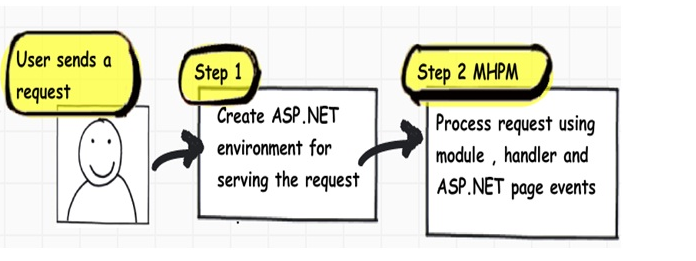
\includegraphics[scale=0.8]{IISHandleUserRequest.png}
	\caption{IIS处理请求过程}
	\label{fig:IISHandleUserRequest}
\end{figure}

\begin{figure}[htbp]
	\centering
	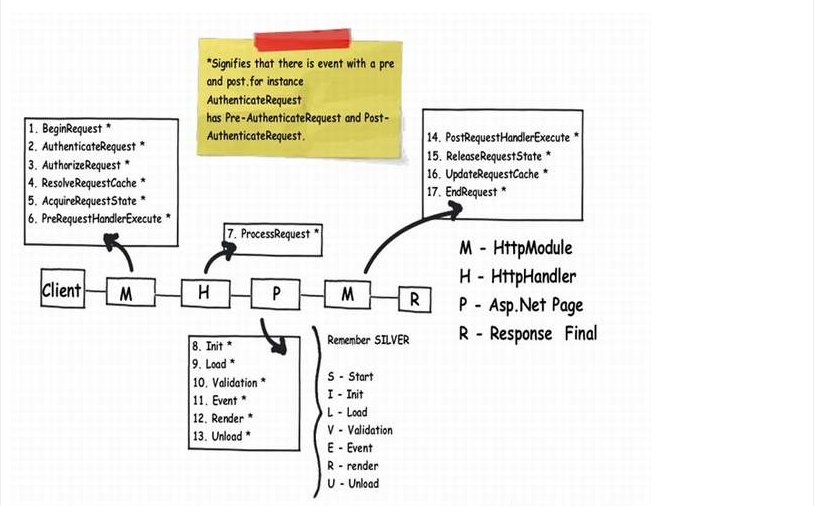
\includegraphics[scale=0.8]{TheWholeLifeCycleOfHttp.png}
	\caption{ASP.NET生命周期}
	\label{fig:TheWholeLifeCycleOfHttp}
\end{figure}
http://www.cnblogs.com/suizhouqiwei/archive/2012/08/15/2637775.html

\subsection{Chrome使用技巧}

\paragraph{搜索源文件}
如果查找每个文件,一般都是打开控制台,
在source控制面板里面一个一个去找,看下面的图你就应该知道,这么多文件,
你都不知道在哪个目录下面,然后就只能一个一个点开看,
按Ctrl+P(cmd+p on mac),就能快速搜寻和打开你项目的文件。

Normal reload:
The same thing as pressing F5. This will use the cache but revalidate everything during page load, 
looking for "304 Not Modified" responses. If the browser can avoid re-downloading cached JavaScript files, images, text files, etc. then it will.

Hard reload:
Don't use anything in the cache when making the request. Force the browser do re-download every JavaScript file, image, text file, etc.

Empty Cache and Hard Reload:
Obviously if the cache is empty then it will have to do a hard reload. This will again force the browser to re-download everything. 
However, if the page makes any after-the-fact downloads via JavaScript that weren't part of page load, then these might still use the cache, 
which is where emptying the cache helps because it makes sure that even these won't use cached files.

\paragraph{Snippets}
Source下的Snippets,可以让你想保存小段的脚本、书签或是你在浏览器中调试时经常用到的代码,都可以使用Snippets,你可以在Source面板里创建、存储和运行这些Snippets。

\paragraph{Google页面}

打开App页面:chrome://apps/
列出所有可用页面:chrome://chrome-urls/

\section{页面适应多屏}

\subsection{适应手机浏览}

\paragraph{使用meta标签}这也是普遍使用的方法,理论上讲使用这个标签是可以适应所有尺寸的屏幕的,
但是各设备对该标签的解释方式及支持程度不同造成了不能兼容所有浏览器或系统。

\begin{lstlisting}[language=HTML]
<meta name="viewport" content="width=device-width,initial-scale=1.0, minimum-scale=1.0, maximum-scale=1.0, user-scalable=no"/>
\end{lstlisting}



\section{性能(Performance)}

\subsection{网页优化(Website Optimized)}

\paragraph{css文件放在<head>里面,js文件尽量放在页面的底部}~~因为请求js文件是很花费时间,如果放在<head>里面,就会导致页面的 DOM树呈现需要等待js文件加载完成。这也就是为什么很多网站的源码里面看到引用的文件放在最后的原因。

\paragraph{CDN}静态内容(比如图片、CSS、JavaScript、以及其他cookie无关的网页内容)
都应该放在一个不需要使用Cookie的独立域名之上。
因为域名之下如果有Cookie,那么客户端向该域名发出的每次Http请求,
都会附上Cookie内容。这里的一个好方法就是使用“内容分发网络”(Content Delivery Network,CDN)

\paragraph{favicon.ico}确保网站根目录下有favicon.ico文件,
因为即使网页中根本不包括这个文件,浏览器也会自动发出对它的请求。
所以如果这个文件不存在,就会产生大量的404错误,消耗光你的服务器的带宽。

\paragraph{不要在HTML中缩放图片}

\paragraph{把CSS放到顶部}

\subsection{利用反向代理服务器加速和保护应用}

如果 Web 应用运行在一台独立的电脑上,性能问题的解决方案是显而易见的:
换一台更快的电脑,里面加上更多的处理器、内存、快速磁盘阵列等等。
然后在这台新电脑上运行 WordPress 服务、Node.js 应用、Java 应用等等,会比以前快很多。
(如果应用需要访问服务器,方案还是很简单:换两台更快的电脑,用更快速的连接把它们连接起来。)

但电脑速度可能不是问题所在。通常 Web 应用运行缓慢,是由于电脑一直在不同的任务间切换:
同成千上万的客户交互、访问磁盘上的文件、执行应用代码和其它的任务。
应用服务器可能会因为下面这些问题而崩溃 —— 内存耗尽、把很多的数据从内存交换到磁盘上、以及很多请求都在等待一个类似磁盘 I/O 的单个任务。

你应该采用一种完全不同的方式,而不是升级硬件:增加一个反向代理服务器来分担这些任务。
这台反向代理服务器设置在运行应用的电脑之前,用来处理网络流量。只有这台反向代理服务器直接连到网络上,
它和应用服务器通过一个快速的内部网络进行通信。

利用这台反向代理服务器,应用服务器就不用等着和 Web 应用的用户进行交互,它可以专注在建立网页,
并通过反向代理服务器把它们发送到网络上。因为应用服务器不必再等待客户的响应,所以能以最优的速度运行。

增加一台反向代理服务器也增加了 Web 服务器的弹性。如果一台服务器过载了,很容易增加另一台同类型的服务器。
如果一台服务器宕机,也很容易把它换掉。

因为反向代理服务器带来的灵活性,它也成为了很多其它性能提升方法的先决条件,比如:

\textbf{负载均衡}—— 反向代理服务器上运行一个负载均衡器,把流量平均分配给一堆应用服务器。
由于负载均衡器的引入,在增加应用服务器时可以完全不用修改应用程序。

\textbf{缓存静态文件} —— 直接请求的文件,比如图片或者代码文件,可以存在反向代理服务器上,
并直接发送给客户端,这样可以更快地提供服务,分担了应用服务器的负载,可以让应用执行得更快。

\textbf{保护网站} —— 反向代理服务器可以设置较高的安全级别,通过监控进快速识别和响应攻击,这样就可以把应用服务器保护起来。

NGINX 软件是专门设计用做反向代理服务器的,具有上述这些附加功能。NGINX 利用事件驱动处理的方法,
比其它传统的服务器更加高效。NGINX Plus 增加了更多反向代理的高级功能和支持,包含应用程序健康检查、特定请求路由和高级缓存等

http://blog.jobbole.com/94962/

\subsection{增加一个负载均衡器}

增加一个负载均衡器是一个相对简单的改动,而且会大幅度地改善网站的性能和安全性。
你可以利用负载均衡器把业务分配给一些服务器,而不是建造一台更大更强的 Web 核心服务器。
就算应用程序编写得很烂或者扩展性很差,负载均衡器都能提升用户体验而不需要任何其它的改动。

负载均衡器首先是一个反向代理服务器 —— 它接收网络流量,并把请求转交给另一个服务器。
一个窍门就是让负载均衡器支持两台以上的应用服务器,利用一个选择算法在服务器间分配请求。
最简单的方法就是轮询,每个新请求发送给列表中的下一台服务器。其它方法包括把请求发送给活动连接数量最少的服务器。
NGINX Plus 可以在同一台服务器上维持一个给定的用户会话,这个功能被称为会话持久性。

负载均衡器可以极大地改善性能,因为它们避免让一台服务器过载,而其它服务器却处于空闲的状态。
它们也很容易扩展 Web 服务器的能力,增加相对便宜的服务器并确保它们物尽其用。

负载均衡可以运用在很多协议上,包含HTTP、HTTPS、SPDY、HTTP/2、WebSocket、FastCGI、SCGI、uwsgi、memcache,
还有一些应用程序,包含基于 TCP 的应用和 L4 协议。分析 Web 应用使用了什么技术和性能落后在什么地方。

同一台服务器或者用于负载均衡的服务器,还能处理其他任务,
包含 SSL 终端、支持客户端使用的 HTTP/1/x 和 HTTP/2、以及缓存静态文件。

NGINX 通常被用于负载均衡:想了解更多,请参考这些资料,
一篇介绍性的文章、一篇关于配置的文章、一本电子书和相关的网络课程和相关文档。
我们的商业版本(NGINX Plus),支持更多负载均衡的特殊功能,比如基于服务器响应时间的路由规划,
和基于微软 NTLM 协议的负载均衡。(译者注:NTLM 是NT LAN Manager的缩写,NTLM 是 Windows NT 早期版本的标准安全协议。)

\subsection{缓存静态和动态内容}

\section{Electron}

\subsection{安装}

全局安装electron

\begin{lstlisting}[language=Bash]
# Install the ‘electron’ command globally in your \$PATH
npm install electron-prebuilt -g
\end{lstlisting}

在安装时提示如下错误,Downloading electron-v1.2.1-win32-x64.zip
Error: connect ETIMEDOUT 54.231.18.161:443,直接ping IP:54.231.18.161失败,
到环境变量中将下载地址改成淘宝的镜像ID即可:

\begin{lstlisting}
变量名:ELECTRON_MIRROR
变量值:http://npm.taobao.org/mirrors/electron/
\end{lstlisting}

安装打包工具electron-packager

\begin{lstlisting}[language=Bash]
npm install -g electron-packager
\end{lstlisting}

查看npm已经安装的包:

\begin{lstlisting}[language=Bash]
npm ls
npm ls -g
\end{lstlisting}


NodeJS的安装目录在D:/Program Files/nodejs.


\subsection{第一个程序}

\paragraph{Error: Cannot find module 'app'}明确全局模块的默认安装位置:npm root -g
接着查看全局模块的默认搜索路径:

\begin{lstlisting}[language=Bash]
node
global.module.paths
\end{lstlisting}




\subsection{打包}




\section{常见问题}

\subsubsection{IIS 6中log4net不写日志}

IIS 6默认运行在Network Service账户下,
尝试添加Network Service账户对日志文件夹的读写权限。

\subsubsection{HTTP 错误 500.23 - Internal Server Error检测到在集成的托管管道模式下不适用的ASP.NET设置。}
取消集成模式验证配置:
\begin{lstlisting}[language=HTML]
<system.webServer>  
    <validation validateIntegratedModeConfiguration="false" />
</system.webServer>
\end{lstlisting}

\subsubsection{HTTP 403 - 您无权查看该网页}

每次浏览网页的时候只显示目录,
或者提示你无权查看该网页。
在配置里添加了aspnet\_isapi.dll后,
问题解决,如图\ref{fig:HTTP403ErrorSolution}所示。

\begin{figure}[htbp]
	\centering
	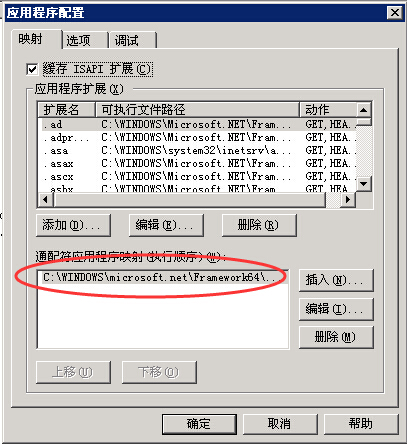
\includegraphics[scale=0.8]{HTTP403ErrorSolution.jpg}
	\caption{HTTP 403您无权查看该网页}
	\label{fig:HTTP403ErrorSolution}
\end{figure}

\subsubsection{HTTP 错误 404.2 - Not Found 由于 Web 服务器上的“ISAPI 和 CGI 限制”列表设置,无法提供您请求的页面。}

如图\ref{fig:ISAPIAndCGI}所示:

\begin{figure}[htbp]
	\centering
	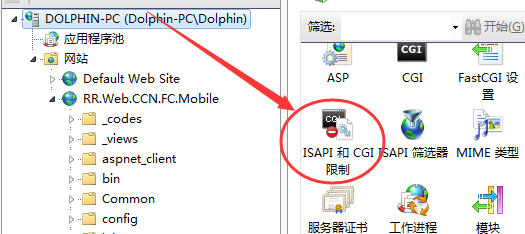
\includegraphics[scale=0.8]{ISAPIAndCGI.png}
	\caption{HTTP错误 404.2}
	\label{fig:ISAPIAndCGI}
\end{figure}

打开IIS7.5,左侧选择根节点,在功能视图中找到"ISAPI和CGI限制"并打开,
将网站应用程序池对应.NET Framework版本设置为允许即可。

\subsubsection{aJax提交500错误}

在aJax提交后返回500错误,后台调试未发现问题,
可将请求URL贴入浏览器地址查看具体信息,
打开Firebug,切换到网络选项卡,
查看请求失败链接的请求头信息和响应头信息,
如图\ref{fig:CheckRequestAndResponseInfo}所示。

\begin{figure}[htbp]
	\centering
	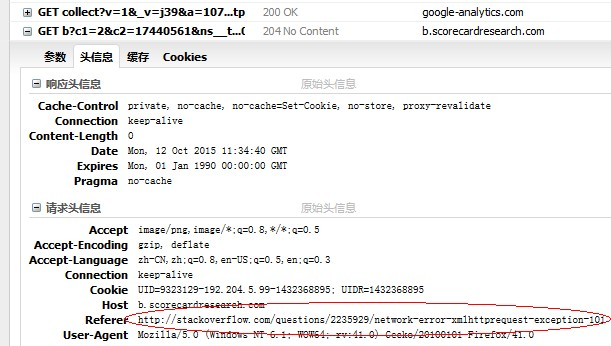
\includegraphics[scale=0.8]{CheckRequestAndResponseInfo.jpg}
	\caption{aJax提交500错误}
	\label{fig:CheckRequestAndResponseInfo}
\end{figure}

将画红框部分贴入浏览器中访问即可发现更加详细的后台错误信息。

\subsection{Bad Request (Invalid Hostname)}

总结页面出现Bad Request (Invalid Hostname)的原因:
1.如果确定域名已经解析生效,但是仍然不能访问,出现Bad Request (Invalid Hostname).那么这就可能是您没有绑定该域名的原因
2.确定端口使用的是80端口

\chapter{Windows Form}

\section{资源文件(Resource)}

\subsection{简介}

资源文件顾名思义就是存放资源的文件。资源文件在程序设计中有着自身独特的优势,
他独立于源程序,这样资源文件就可以被多个程序使用。同时在程序设计的时候,
有时出于安全或者其它方面因素的考虑,把重要东西存放在资源文件中,也可以达到保密、安全的效果。
资源文件中一般存三种类型的数据:byte流(byte[])、对象(object)和字符串(string)。
对于一些纯文件的信息可以用string类型来保存,对于图片(Image)、图标(Icon)等用object来保存,其它的可以用byte流来保存。
System.Resources命名空间中有大量的类和方法来处理资源文件。

\subsection{资源文件的分类}

资源文件可以分为两类,一类是以.resx为后缀名的文件,一类是以.resources为后缀名的文件。
二者的区别在于:

1.resx虽然是以resx结尾的文件,但是它却是XML格式的文件,你可以用记事本等工具直接打开它修改里面的东西;
而resources是二进制的文件,相对来说安全性更好一些。

2.resources作为内嵌资源,在指定路径正确的前提下,
可以在程序中直接引用;而resx虽然也是内嵌资源,但它却是要依附于.CS文件存在的。
也就是说它是作为winform窗体的一个描述性资源存在的,要想在程序中直接使用它,
在解决方案中必须有与它同名(只是名字相同,后缀名不同)的.CS文件存在.

3.可以利用CSC命令把resx文件转换成resources文件。
RESGEN.EXE LitwareStrings.resx LitwareStrings.resources.
注意变量环境为framework1.1。

\subsection{利用资源文件来做多国语言版本}

如何使用VS的IDE来制作多国语言版本。每一个Form1.cs文件都有一或多个相应的resx文件作为附属资源。
他们的命名规则为Form1.cs的资源文件为Form1.resx,Form1.zh-CHS.resx,Form1.zh-CHT.resx等,
其中Form1.resx是缺省的窗体资源文档,其它是在不同语言环境要使用的资源文档,
其中Form1.zh-CHS.resx是中文简体系统,Form1.zh-CHT.resx是中文繁体系统。
关于命名可不是随便起的,可以参见msdn中关于不同地区的命名规则。

\subsection{MouseDown事件后无法触发MouseDoubleClick}

.NET控件的单双击事件的触发过程,就是先触发单击过程,再触发双击过程
这个是.NET已有控件的固定机制,这个无法改变。
事件引发的顺序:
MouseDown 事件。
Click 事件。
MouseClick 事件。
MouseUp 事件。
MouseDown 事件。
DoubleClick 事件。
MouseDoubleClick 事件。
MouseUp 事件。

\subsection{指定DllImport文件目录}

引用的dll都放在根目录下,随着项目的日益增大,根目录下充满了各种各样的dll,非常的不美观。
如果能够把dll按照想要的目录来存放,那么系统就美观多了,
有时需要引用Win32的Native dll,无法通过定义私有目录的方式定义dll,
此时可以通过指定程序的环境变量的方式定义dll的搜索目录,
添加环境变量的代码如下片段所示。

\begin{lstlisting}[language={[Sharp]C}]
public static void AddEnvironmentPaths(IEnumerable<string> paths)
{
	var path = new[] { Environment.GetEnvironmentVariable("PATH") ?? string.Empty };
	var newPath = string.Join(Path.PathSeparator.ToString(), path.Concat(paths));
	Environment.SetEnvironmentVariable("PATH", newPath);
}
\end{lstlisting}

这样添加环境变量对系统的环境变量没有影响。

\subsection{窗口句柄}

在Windows中,句柄是一个系统内部数据结构的引用。例如当你操作一个窗口,或说是一个Delphi窗体时,
系统会给你一个该窗口的句柄,系统会通知你:你正在操作142号窗口,
就此你的应用程序就能要求系统对142号窗口进行操作——移动窗口、改变窗口大小、把窗口最小化等等。
实际上许多Windows API函数把句柄作为它的第一个参数,如GDI(图形设备接口)句柄、菜单句柄、实例句柄、位图句柄等,
不仅仅局限于窗口函数。换句话说,句柄是一种内部代码,通过它能引用受系统控制的特殊元素,如窗口、位图、图标、内存块、光标、字体、菜单等。

\subsection{Windows弹出窗体}

将最小化窗体弹出并置于最前端。

\begin{lstlisting}[language={[Sharp]C}]
frmBatchSendMessage.Show();
if (frmBatchSendMessage.WindowState == FormWindowState.Minimized)
{
	frmBatchSendMessage.WindowState = FormWindowState.Normal;
}
frmBatchSendMessage.Activate();
\end{lstlisting}

\paragraph{MessageBox}MessageBox的关闭按钮在MessageBoxButtons为YesNo枚举类型时不可用,
可以采用MessageBoxButtons.OKCancel,如果想让MessageBox始终置于窗体的最前端,
MessageBoxOptions使用DefaultDesktopOnly属性。如代码所示:

\begin{lstlisting}[language={[Sharp]C}]
var result = MessageBox.Show(\@"系统检测到新版本,是否升级", \@"更新提示", MessageBoxButtons.OKCancel, MessageBoxIcon.Information, MessageBoxDefaultButton.Button1, MessageBoxOptions.DefaultDesktopOnly);  // MB\_TOPMOST
\end{lstlisting}

\section{常见问题}

\subsection{关于嵌入互操作类型(Embed Interop Types)}

在项目开发中引用了一个dll,编译器显示警告如下:

\begin{lstlisting}
由于存在对由程序集“AxInterop.videocx3Lib.dll”创建的程序集的间接引用,因此创建了对嵌入的互操作程序集“Interop.videocx3Lib.dll”的引用。请考虑更改其中一个程序集的“嵌入互操作类型”属性。
\end{lstlisting}

当按照提示更改AxInterop.videocx3Lib.dll的嵌入互操作类型后出现错误:

\begin{lstlisting}
无法嵌入来自程序集“AxInterop.videocx3Lib.dll”的互操作类型,因为它缺少“ImportedFromTypeLibAttribute”特性或“PrimaryInteropAssemblyAttribute”特性
\end{lstlisting}

排查发现此程序集和另一个ActiveX组件存在冲突,
更改ActiveX组件的嵌入互操作类型后问题得以解决。
使用 COM 互操作程序集,而不要求该程序集在运行时必须存在。
目的是减轻将 COM 互操作程序集与您的应用程序一起部署的负担。
"嵌入互操作类型"中的嵌入就是引进、导入的意思,
类似于c\#中using,c中include,Java的Import的作用,目的是告诉编译器是否要把互操作类型引入。
"互操作类型"实际是指一系列Com组件的程序集,是公共运行库中库文件,类似于编译好的类,接口等。
"嵌入互操作类型"设定为true,实际上就是不引入互操作集(编译时候放弃Com程序集),仅编译用户代码的程序集。
而设定为false的话,实际就是需要从互操作程序集中获取 COM 类型的类型信息。
当 COM 互操作在最初版本的 .NET Framework 中引入时,就确立了主互操作程序集 (PIA) 的概念。
引入此概念,是为了解决在组件之间共享 COM 对象的难题。例如:如果您有一些不同的互操作程序集,
分别定义了一个 Excel Worksheet,则我们无法在组件之间共享这些 Worksheet,因为它们具有不同的 .NET 类型。
PIA 通过只存在一次而解决了这个难题:所有客户端都使用它,因此 .NET 类型始终是匹配的。
尽管 PIA 在理论上是个好主意,但在实际部署中却被证明是个大麻烦,因为它只有一份,而有多个应用程序可能会尝试安装或卸载它。
而由于 PIA 通常很大,事情更复杂了。Office 在默认 Office 安装方式中并未部署它们,
用户只需通过使用 TLBIMP 来创建自己的互操作程序集,即可轻松绕过这一个程序集系统。
因此,现在为了扭转这种局面,发生了两件事:
对于两个结构相同且共享相同识别特征(名称、GUID等)的COM互操作类型,运行时能够聪明地将其看作同一个 .NET 类型。
C\#编译器利用这一点的方式是在编译时直接在您自己的程序集中重现互操作类型,因此不再要求在运行时存在该互操作程序集。
通过将引用上的“嵌入式互操作类型”属性设置为 true,告诉编译器为您将互操作类型嵌入到 Visual Studio 中。
由于C\#团队希望这种方法成为引用COM程序集的首选方法,因此在默认情况下,
Visual Studio会将添加到C\#项目中的任何新互操作引用的此属性设置为True(这里不准确,经过测试添加的dll嵌入互操作类型的值为False)。
Beginning with the .NET Framework 4, the common language runtime supports embedding type 
information for COM types directly into managed assemblies, 
instead of requiring the managed assemblies to obtain type information for COM types from interop assemblies.  
Because the embedded type information includes only the types and members that are actually used by a managed assembly, 
two managed assemblies might have very different views of the same COM type.  
Each managed assembly has a different Type object to represent its view of the COM type.  
The common language runtime supports type equivalence between these different views for interfaces,
 structures, enumerations, and delegates.  

\subsection{Class not registered}

Class not registered (Exception from HRESULT: 0x80040154 (REGDB\_E\_CLASSNOTREG))

\subsection{试图加载格式不正确的程序}

在Manage Code中加载Native dll程序时出错,错误如下:

\begin{lstlisting}[language={[Sharp]C}]
“System.BadImageFormatException”类型的第一次机会异常在 MVSP.Common.dll 中发生
其他信息: 试图加载格式不正确的程序。 (异常来自 HRESULT:0x8007000B)
\end{lstlisting}

程序在64位的机器上就会用运行为64位,而64程序是不能加载32位dll的。
dll文件是在64位开发环境下下编译的,而你现在的调用程序是的32位,所以无法调用。

\subsection{Dictionary索引超出数组界限}

在向Dictionary中添加项时提示此错误,
原因是程序是多线程,Directory不是线程安全的,
解决方案是添加lock语句。

\begin{lstlisting}[language={[Sharp]C}]
lock (DataManager.VehicleLatestAlarmInfoList)
{
	if (!DataManager.VehicleLatestAlarmInfoList.ContainsKey(vehicleInfo.VehicleID))
	{
		DataManager.VehicleLatestAlarmInfoList.Add(vehicleInfo.VehicleID, DateTime.Now);
	}
	else
	{
		DataManager.VehicleLatestAlarmInfoList[vehicleInfo.VehicleID] = DateTime.Now;
	}
}
\end{lstlisting}

\begin{lstlisting}[language=Python]
import string
\end{lstlisting}

\subsection{System.ComponentModel.Design.ExceptionCollection}

在Visual Studio打开设计器时提示此错误,
The real problem of the "ExceptionCollection" being thrown is that when there is a WSOD (White Screen of Darn) indicating a designer load issue, 
the designer gets unloaded. In your project, the RussTabStrip is throwing exceptions. 
These get caught by our unload method and get displayed in the dialog box you see.
So, to fix this you should:

1) Start a second instance of visual studio
2) go the the Tools menu, "Attach to process", select the 'devenv.exe' process, and click the 'attach' button.
3) In the Debug/Exceptions menu 
4) Open the designer with the debugger attached
5) The second visual studio will break on your error.

\subsection{程序点击无反应}

如果是在客户的环境上,可以尝试使用dnSpy等反编译工具调试编译完成的dll。

\subsection{程序的界面显示异常}

检查操作系统的字体设置(控制面板/外观和个性化/显示)。

\chapter{ASP.NET MVC(Apache License 2.0)}

MVC模型以低耦合、可重用、可维护性高等众多优点已逐渐代替了WebForm模型。

\clearpage
\mbox{}         
\clearpage

\section{MVC权限}

\subsection{MVC登录验证}

有时有的网页需要用户登录才能够操作,
所以需要进行用户是否登录的验证。
基本思路是用户登录后Cookie里存放一个值,
当再次请求时判断此值是否存在,
存在就代表已经登录。
编写过滤器ActionExecuteFilter继承ActionFilterAttribute在每一个Action执行之前判断用户是否已经登录:

\begin{lstlisting}[language={[Sharp]C}]
public class ActionExecuteFilter : ActionFilterAttribute
{
    public override void OnActionExecuting(ActionExecutingContext filterContext)
    {
        //OnActionExecuting:正要准备执行Action的时候但还未执行时执行
        var userId = filterContext.HttpContext.Request.Cookies["userId"];
        if (userId != null) return;
        var controllerName = (string)filterContext.RouteData.Values["controller"];
        if (controllerName != "Login")
        {
            //跳转到登陆页
            filterContext.Result = new RedirectResult("/Login/Index");
        }
    }
}
\end{lstlisting}

用户登录时设置Cookie,下一次请求时Cookie将通过HTTP发送到服务端。

\begin{lstlisting}[language={[Sharp]C}]
public JsonResult SignIn(string input1, string input2)
{
    var loginSuccess = false;
    if (input1 == "doc" && input2 == "doc")
    {
        var cookie = new HttpCookie("userId", "1");
        Response.Cookies.Add(cookie);
        loginSuccess = true;
    }
    return new JsonResult { Data = loginSuccess, JsonRequestBehavior = JsonRequestBehavior.AllowGet };
}
\end{lstlisting}

\section{MVC生命周期}

\subsection{ASP.NET MVC的处理流程}

当我们访问http://localhost:8080/Home/Index 这个地址的时候,请求首先被UrlRoutingModule截获,
截获请求后,从Routes中得到与当前请求URL相符合的RouteData对象, 
将RouteData对象和当前URL封装成一个RequestContext对象,然后从Requestcontext封装的RouteData中得到 Controller名字,
根据Controller的名字,通过反射创建控制器对象,这个时候控制器才真正被激活,最后去执行控制器里面对应的 action。

处理流程:
1.用户发起请求---》UrlRouting获取请求—》MvcRouteHandler.GetHttpHandler()—>MvcHandler.ProcessRequest()

2.UrlRouting获取浏览器发起的请求后将RoutData与HttpContext合并成为RequestContext传递到IRoutHandler接口,IRoutHandler接口的实现类MvcRouteHandler接口到RequestContext参数,
返回一个MvcHandler对象,并且为这个对象赋值RequestContext

\paragraph{MvcHandler对象}
根据Controller的名字正确的实例化了一个Controller对象后。
回到MvcHandler(System.Web.Mvc.MvcHandler)的BeginProcessRequest方法,
可以看到,
当得到Controller对象之后,首先判断它是不是IAsyncController,
如果是则会创建委托用来异步执行。通常情况下,我们都是继承自Controller类,
这不是一个IAsyncController,于是会直接执行Controller的Execute方法。
Execute方法是在Controller的基类ControllerBase中定义的,
这个方法除去一些安全检查,
初始化了ControllerContext(包含了ControllerBase和Request的信息),
核心是调用了ExecuteCore(System.Web.Mvc.Controller.ExecuteCore)方法。
根据RequestContext参数解析出RouteData以及HttpContext,
根据RouteData来查找出Controller以及对象的Action及其Parameters。
在每次执行action时(System.Web.Mvc.ControllerActionInvoker类下的InvokeAction方法)都会找出过滤器一并执行,核心语句为:

\begin{lstlisting}[language={[Sharp]C}]
FilterInfo filters = this.GetFilters(controllerContext, action);
\end{lstlisting}

这就是过滤器的执行时机,在应用程序启动的时候全局注册过滤器,
在每次Request的时候执行过滤器,对于权限控制,
日志记录等需要面向切面(AOP:Aspect Oriented Programming)的业务来说是非常合适的。

5.Controller.Execute()方法处理流程:查找Action-->
获取Action--->调用ActionResult(Abstract方法)的ActionResult.ExecuteResult()方法

6.ActionResult.ExecuteResult()方法

获取到IView对象,--》根据Iview对象的页面路径获取到具体的Page,
--->调用IView.RenderView()方法显示页面,
IView对象中存储的是页面的路径地址,
最终通过页面引擎(View Engine)使用该路径生成具体的页面类,
ViewPage(System.Web.Mvc.ViewPage)是实现了IView接口的对象。

7,最终页面就可以正确的显示。

ViewPage.RenderPartialView()显示.ascx文件或者是ViewPage.RenderView()显示.aspx文件。
现在MVC 3中使用的是Razor视图引擎,和WebFormViewEngine一样的处理流程
下面附上Pro Asp.net MVC的作者的一副图,
如图\ref{fig:ASP.NETMVCRequestHandlingPipelinethumb}所示。

\begin{figure}[htbp]
	\centering
	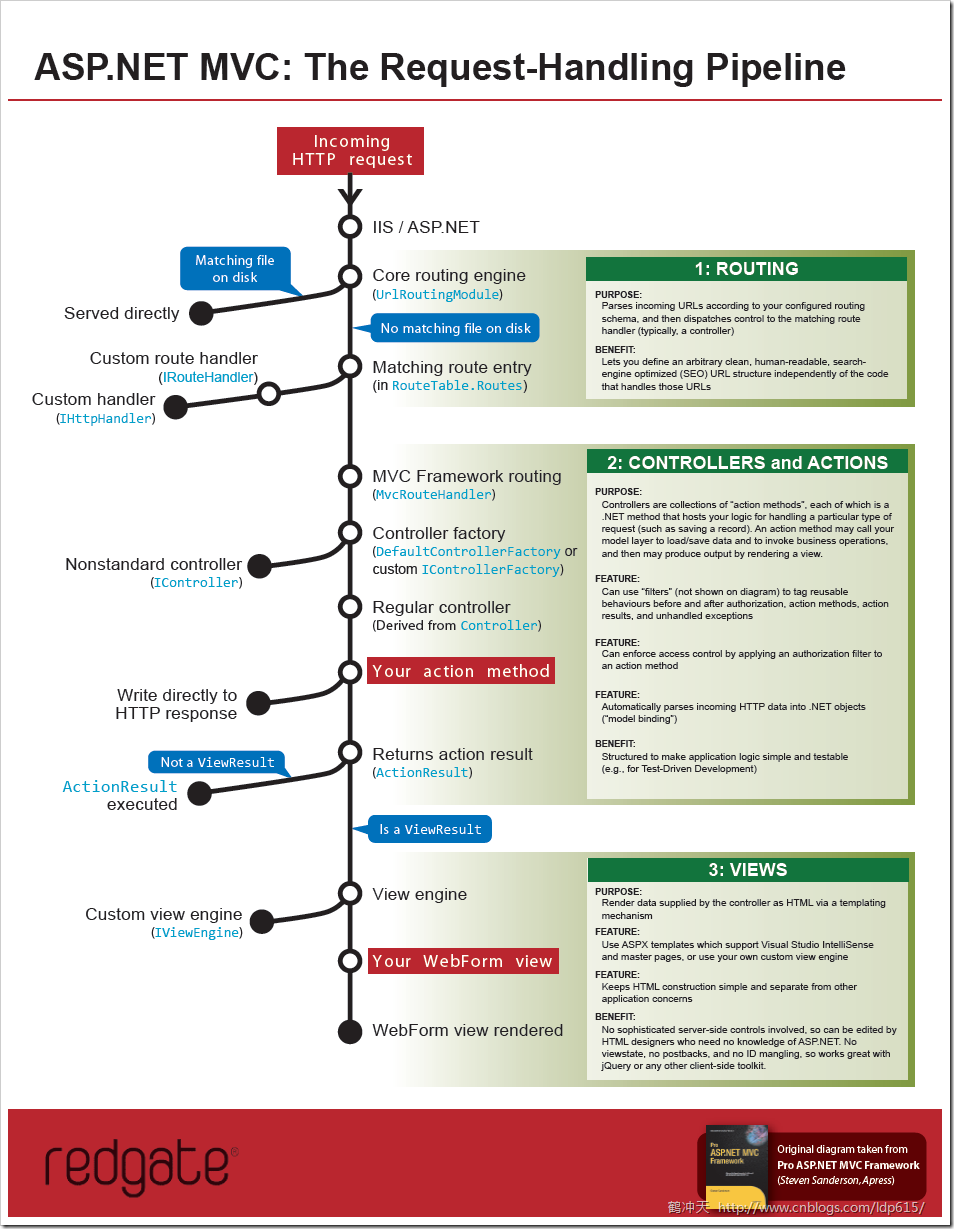
\includegraphics[scale=0.6]{ASP.NETMVCRequestHandlingPipelinethumb.png}
	\caption{MVC中HTTP请求的处理过程}
	\label{fig:ASP.NETMVCRequestHandlingPipelinethumb}
\end{figure}

\subsection{ASP.NET请求生命周期(ASP.NET MVC Request Life Cycle)}

\subsubsection{RouteTable(路由表)的创建}

MVC路由表的创建在站点开始启动之后,将站点的所有路由缓存到内存中,
当截获Request请求时,从内存中进行匹配。

\subsubsection{UrlRoutingModule请求拦截}

The request is first intercepted by the UrlRoutingModule which is a HTTP Module. 
It is this module that decides whether the request would be handled by our MVC application. UrlRouting Module selects the first matching route. 

3)Routing engine 确定route

4)route handler 创建相关的IHttpHandler实例

5)IHttpHandler实例确定Controller(控制器)

6)Controller执行

7)一个视图引擎创建

8) 视图呈现

\subsection{路由忽略}

在MVC的路由配置中,有如下语句:

\begin{lstlisting}[language={[Sharp]C}]
routes.IgnoreRoute("{resource}.axd/{*pathInfo}");
\end{lstlisting}

表示对于*.axd类型的链接将不进行路由。
axd files are typically implemented as HTTP Handlers. 
They don't exist as an ASP.NET web page, 
but rather as a class that implements the IHttpHandler interface.
*.axd类型的链接主要用于获得嵌入到dll中的资源,
The answer is WebResource.axd. WebResource.
axd is an HTTP Handler that is part of the .NET Framework that does one 
thing and one thing only – it is tasked with getting an 
embedded resource out of a DLL and returning its content. 
What DLL to go to and what embedded resource to take are specified through the querystring. 
For instance, a request to www.yoursite.com/WebResource.axd?d=EqSMS…\&amp;t=63421… might return a particular snippet of JavaScript embedded in a particular assembly. 
The d querystring parameter contains encrypted information that specifies the assembly and resource to return; 
the t querystring parameter is a timestamp and is used to only allow 
requests to that resource using that URL for a certain window of time.
详情参考\url{http://scottonwriting.net/sowblog/archive/2010/10/28/just-where-is-webresource-axd.aspx}。

\subsection{Controller的激活过程(Process of Controller Activation)}

RouteData从Url中获取Controller的名称
(具体可参见Route类的GetRouteData方法),
MVC从RouteData(在C:/Windows/Microsoft.NET/Framework/v4.0.30319文件夹下
的System.Web.dll中)中获取Controller的名称,
通过ControllerFactory传入Controller名称激活Controller。
第一步由Controller的名称获取Controller的类型实例。
代码如片段\ref{code:GetTypeInstanceByControllerName}所示:

\begin{lstlisting}[language={[Sharp]C},caption=由Controller名称获取类型实例,label={code:GetTypeInstanceByControllerName}]
private Type GetControllerTypeWithinNamespaces(RouteBase route, string controllerName, HashSet<string> namespaces)
{
   this.ControllerTypeCache.EnsureInitialized(this.BuildManager);
   //由Controller名称和命名空间获取类型实例
   ICollection<Type> controllerTypes = this.ControllerTypeCache.GetControllerTypes(controllerName, namespaces);
   switch (controllerTypes.Count)
   {
     case 0:
       return (Type) null;
     case 1:
       return Enumerable.First<Type>((IEnumerable<Type>) controllerTypes);
     default:
       throw DefaultControllerFactory.CreateAmbiguousControllerException(route, controllerName, controllerTypes);
   }
}
\end{lstlisting}

ControllerFactory的作用是创建为请求提供服务的Controller实例;
在获取实例的过程中利用了反射,由类的名称获取类型实例就是典型的反射。
反射可以增加程序的可扩展性与灵活性,同时也会降低程序的性能。
简单的由类的名称获取类型实例以及类的实例示例代码如片段\ref{code:GetClassInstanceUsingReflection}所示:

\begin{lstlisting}[language={[Sharp]C},caption=反射获取类的实例示例,label={code:GetClassInstanceUsingReflection}]
//定义一个类,包含一个公共的名称属性
public class Demo
{
    public string Name = "Dolphin";
}

//通过反射获取类型实例
Type demoTypeInstance = Type.GetType("MvcApplication1.Controllers.Demo,MvcApplication1");
if (demoTypeInstance != null)
{
	//获取Demo类的实例
    Demo demoInstance = (Demo)Activator.CreateInstance(demoTypeInstance);
    string name = demoInstance.Name;//name的值为:Dolphin
}
\end{lstlisting}

在GetType方法中,参数由命名空间和程序集组合而成,中间以逗号隔开,
逗号前是命名空间和类名,逗号后是程序集的名称。
Type为System.Reflection功能的根,也是访问元数据的主要方式。
使用Type的成员获取关于类型声明的信息,如构造函数、方法、字段、属性 (Property) 和类的事件,
以及在其中部署该类的模块和程序集。
MVC的激活过程即是如此过程,在MVC中通过类型实例激活类实例如代码片段\ref{code:GetControllerInstanceUsingReflection}所示。

\begin{lstlisting}[language={[Sharp]C},caption=MVC获取类的实例,label={code:GetControllerInstanceUsingReflection}]
public IController Create(RequestContext requestContext, Type controllerType)
{
   try
   {
     return (IController) (this._resolverThunk().GetService(controllerType) ?? Activator.CreateInstance(controllerType));
   }
   catch (Exception ex)
   {
      throw new InvalidOperationException(string.Format((IFormatProvider) CultureInfo.CurrentCulture, MvcResources.DefaultControllerFactory_ErrorCreatingController, new object[1]
      {
        (object) controllerType
      }), ex);
   }
}
\end{lstlisting}

ActionInvoker的作用是寻找并调用Action方法。


\section{MVC页面传值}

\subsection{(View \textrightarrow ~Controller)}
~MVC中通过AJax的POST方式向Controller传值如下代码所示:

\begin{lstlisting}[language=VBScript]
$(function () {
    $("#debuggerSubmit").click(function () {        
        $.post(
            "/User/GetUserAwardTypeCountDebugger",
            {
                action: "post",
                UserID: $("UserID").val(),
                UserName: $("AwardType").val()
            },
            function (data) {
                alert("OK");
            });
    });
});
\end{lstlisting}

UserID将页面控件ID为UserID的控件值传入后台的Controller页面,
在Controller页面的接收如下代码片段所示(post采用Request.Form的方式获取值,
服务端获取POST方式传递的参数采用此种写法,
服务端获取Get请求参数用Request.QueryString):

\begin{lstlisting}[language={[Sharp]C}]
public ActionResult GetUserAwardTypeCountDebugger()
{
    int userID = Convert.ToInt32(Request.Form["UserID"]);    
    return Content("OK");
}
\end{lstlisting}

\paragraph{使用ajaxSubmit}~~ajaxSubmit(obj)方法是jQuery的一个插件jquery.form.js里面的方法,所以使用此方法需要先引入这个插件。

\begin{lstlisting}[language=VBScript]
$(".right").bind("click", function () {
    $("form[method='post']").submit();
});

//bind()和delegate()都是由on()实现
$(document).on("submit", "form[method='post']", function () {
    $(this).ajaxSubmit(function (m) {
        var json = m;
        if (!json.status) {
            alert(json.message);//出错,弹出错误提示
        } else {
            var arrData = json.data.split("|");
            var calllbackUrl = "http://m.tour.zouwo.com/Order/Index?orderid=" + json.data;
            var url = "@(PayUrl)id=" + arrData[0] + "&url=" + calllbackUrl + "";
            window.location.href = url;
        }
    });
    return false;
});
\end{lstlisting}

后端定义相应的模型(Model),通过模型绑定的方式接收前端的传值。
on()的描述:

\begin{lstlisting}[language=VBScript]
.on( events [, selector ] [, data ], handler(eventObject))
\end{lstlisting}

事件冒泡通过大量祖先元素会导致较大的性能损失。而使用.on()方法,
事件只会绑定到\$()函数的选择符表达式匹配的元素上(上面我的例子中,
为了简单绑定到了document),因此可以精确地定位到页面中的一部分,而事件冒泡的开销也可以减少。

\paragraph{POST传值(View与Controller互传)}~

在MVC控制器传递多个Model到视图,
可使用ViewData, ViewBag, PartialView, TempData, ViewModel, Tuple。
PartialView是对于哪些需要重复使用的视图部分,提取出来作为部分视图。

View向Controller传值如下代码所示:

\begin{lstlisting}
<script>
    $(function () {
        $("#debuggerSubmit").click(function () {               
            $.ajax({
                type: 'POST',
                async: false,
                url: "/User/GetUserAwardTypeCountDebugger",
                data: 
                {
                    action: "post",
                    UserID: $("#UserID").val(),
                    UserName: $("#AwardType").val()
                },
                success: function (data) {
                    $("#ajax_msg").html(data);
                }
            });
        });
    });
</script>
\end{lstlisting}

其中url中的User为View的cshtml页面的上级文件夹名称,
GetUserAwardTypeCountDebugger为Controller中相应的方法的名称。
在Controller中接收参数和回传参数如下代码所示:

\begin{lstlisting}[language={[Sharp]C}]
[HttpPost]
public JsonResult GetUserAwardTypeCountDebugger()
{
    int userID = Convert.ToInt32(Request.Form["UserID"]);
    string a = "回传值";
    return new JsonResult { Data=a, JsonRequestBehavior= JsonRequestBehavior.AllowGet};
}
\end{lstlisting}

回传值通过JsonResult类的Data进行回传,
在前端cshtml界面中通过ajax调用的sucess进行参数的接收。
方法的HttpPost属性代表此方法只处理POST请求,
防止无意间调用,相当于增加了方法的使用约束,增加安全性。
可以添加ValidateAntiForgeryToken属性防止跨站请求伪造CSRF(Cross-site Request Forgery)攻击,
相应的在页面的开头需要添加@Html.AntiForgeryToken()。
\subparagraph{title}

form元素中的子元素可以直接使用,
在Controller中可以直接通过Request.Form直接获取元素的值。
form的写法如下:

\begin{lstlisting}[language=HTML]
<form name="" action="/Product/PickAward" method="post" enctype="multipart/form-data">
    <p>
        <label>用户ID:</label>
        <input type="text" id="userId" name="userId" class="form-control" placeholder="用户ID"/>
    </p>
</form>
\end{lstlisting}

form元素注明为post,action为Controller中相应的方法的名称。
在Controller中接收参数通过如下语句接收参数:

\begin{lstlisting}[language={[Sharp]C}]
int userId = int.Parse(Request.Form["userId"].ToString());
\end{lstlisting}

由Controller向View传递参数可在服务端采用return View(model)语句,
在前端页面通过Model进行接收。

\begin{lstlisting}[language={[Sharp]C}]
@model DBCCN.Model.discount_sellerModel
@using RR.Web.CCN.FC.Common
@{
    ViewBag.Title = "";
    Layout = "~/Views/Shared/_Layout.cshtml";
    string staticPath = PublicAttribute.staticPath;
    string themeVersion = PublicAttribute.themeVersion;   
}
\end{lstlisting}

\subsubsection{MVC传递全局变量}

通过Session和Cookie传值。

\subsection{PageRouteHandler vs MvcRouteHandler}

地址路由功能并不是MVC特有的,在ASP.NET中为PageRouteHandler,
在MVC中为MvcRouteHandler。
对于调用RouteCollection的GetRouteData获得的RouteData对象,
其RouteHandler来源于匹配的Route对象。
对于通过调用RouteCollection的MapPageRoute方法注册的Route来说,
它的RouteHandler是一个类型为PageRouteHandler对象。
由于调用MapPageRoute方法的目的在于实现请求地址与某个。
aspx页面文件之间的映射,所以我们最终还是要创建的Page对象还处理相应的请求,
所以PageRouteHandler的GetHttpHandler方法最终返回的就是针对映射页面文件路径的Page对象。
ASP.NET MVC的Route对象是通过调用RouteCollection的扩展方法MapRoute方法进行注册的,
它对应的RouteHandler是一个类型为MvcRouteHandler的对象。如下面的代码片断所示,
MvcRouteHandler用于获取处理当前请求的HttpHandler是一个MvcHandler对象。
MvcHandler实现对Controller的激活、Action方法的执行以及对请求的相应,
毫不夸张地说,整个MVC框架实现在MvcHandler之中。

\begin{lstlisting}[language={[Sharp]C}]
public class MvcRouteHandler : IRouteHandler
{
	IHttpHandler IRouteHandler.GetHttpHandler(RequestContext requestContext)
	{
		return GetHttpHandler(requestContext);
	}
}
\end{lstlisting}

如果url是 /home/index?id=3 直接Request就ok。
但是如果路由设定为:{controller}/{action}/{id} 
url是 /home/index/3   
这时想在页面View中获取参数id的值,该怎么获取?
 
一种方式可利用Action获取到参数值后,用Viewdata传到View中
例如
Controlers中的phonelist这样定义  
public ActionResult phonelist(int id)  
  {  
  ViewData["id"] = id;   
  return View();  
  }  

其实,有更加简单的方式,只要在view中这样获取就可以:

\begin{lstlisting}[language=HTML]
<%=Html.ViewContext.RouteData.Values["id"]%>
\end{lstlisting}

就算没有id的参数也不会报错。同样:

\begin{lstlisting}[language=HTML]
//写法1
<%=Request.RequestContext.RouteData.Values["id"] %>
//写法2
<%=Html.ViewContext.RouteData.Route.GetRouteData(Html.ViewContext.HttpContext).Values["id"]%>
\end{lstlisting}

也可以取到。
 
注:在用户控件中是无法直接访问到RouteData,RouteData是Page对象中的属性,
所以需要在用户控件中使用this.Page.RouteData来获取参数
使用this.Page.RouteData.Values["id"]来获取参数的值

\section{MVC异常处理(MVC Error Handling)}

在MVC里面,万一在行为方法里面抛出了什么异常的,
而那个行为方法或者控制器有用上HandleError过滤器的,
异常的信息都会在某一个视图显示出来,
这个显示异常信息的视图默认是在Views/Shared/Error。
在应用程序启动的时候就已经注册了全局过滤器,
HandleErrorAttribute就是系统自带的异常过滤器。
在这注册的全局过滤器,可以不用到每个Controller或者是每个Action去声明,
直接作用于全局了,即可以捕捉整个站点的所有异常。
MVC异常处理一般可以在Action级别处理,
也就是当前Action,也可以在Controller级别处理,
包括当前Controller和所有Controller,
还可以在应用程序级别处理,
也就是Application\_Error,如果都不进行处理,
异常将抛给用户。

\subsection{Application\_Error}

程序中发生的所有异常,都可以在这里捕获。
但是有一个不足的地方,那就是,如果我们在这里捕获异常之后,
需要显示错误页面,那么浏览器上的地址是会改变的,已经被重定向了。
也就是说,浏览器上显示的地址,并不是真正发生错误的地址,
而是仅仅是显示错误信息的页面地址。这个不足,
跟在Web.config的customError中配置错误页面是一样的。
很多时候,我们是希望在访问某个URL后发生了错误,
显示错误页面之后,URL还是不变。因此,在这里处理异常并不能满足这种需求。
在Global.asax代码片段\ref{code:ApplicationLevelErrorHandler}代码是在程序级别捕获错误。

\begin{lstlisting}[language={[Sharp]C},caption=MVC应用程序级别错误处理,label=code:ApplicationLevelErrorHandler]
void Application_Error(object sender, EventArgs e)
{     
    var exception = Server.GetLastError().GetBaseException();
    var errorDetail = new StringBuilder();
    errorDetail.Append("\r\n" + DateTime.Now.ToString("yyyy.MM.dd HH:mm:ss"));
    errorDetail.Append("\r\n.客户信息:");
    var serverIp = Request.ServerVariables.Get("HTTP_X_FORWARDED_FOR");
    var remoteAddr = Request.ServerVariables.Get("Remote_Addr").Trim();
    var ipAddress = (serverIp != null) ? serverIp.Trim() : remoteAddr;
    errorDetail.Append("\r\n\tIp:" + ipAddress);
    errorDetail.Append("\r\n\t浏览器:" + Request.Browser.Browser);
    errorDetail.Append("\r\n\t浏览器版本:" + Request.Browser.MajorVersion);
    errorDetail.Append("\r\n\t操作系统:" + Request.Browser.Platform);
    errorDetail.Append("\r\n.错误信息:");
    errorDetail.Append("\r\n\t页面:" + Request.Url);
    errorDetail.Append("\r\n\t错误信息:" + exception.Message);
    errorDetail.Append("\r\n\t错误源:" + exception.Source);
    errorDetail.Append("\r\n\t异常方法:" + exception.TargetSite);
    errorDetail.Append("\r\n\t堆栈信息:" + exception.StackTrace);
    errorDetail.Append("\r\n-------------------------------------------------");
    PublicAttribute.Logger.Error(errorDetail);
    //处理完及时清理异常 
    Server.ClearError();
    //跳转至友好的出错页面 
    Response.Redirect(@"~/error/index");
}
\end{lstlisting}

\subsection{OnException继承HandleErrorAttribute}

MVC的特点就是,每一个请求都对应一个Controller,
当在某个Controller中发生异常时,我们都可以在OnException中捕获。
但是,如果根本就找不到这个Controller,那么这种错误OnException就无能为力了。举个例子:
假设有个Controller叫About,当访问http://host/About/Index发生错误时,
是可以在OnException中捕获的。但如果我访问http://host/Aboute/Index的时候,
因为根本不存在Aboute控制器,所以这种错误是无法在OnException捕获的,
如果要捕获这种错误,只能在Application\_Error中处理。
虽然OnException不能捕获所有的错误,但是,
它可以解决Application\_Error错误页面重定向的问题,在显示错误页面的时候,URL保持不变。
在Web.config文件中添加配置如代码片段\ref{code:MVCErrorHandler}所示。

\begin{lstlisting}[language=XML,caption=配置MVC错误处理页面,label=code:MVCErrorHandler]
<System.Web>
	<customErrors mode="On" defaultRedirect="/Error/Index" />
</System.Web>
\end{lstlisting}

如果在当前Controller中重写OnException方法,
那么当前Controller中的Action抛出异常后交由当前Controller中重写的OnException方法处理,
如果继承HandleErrorAttribute并重写OnException方法,
那么可以处理所有Controller抛出的异常,如代码片段\ref{code:UserDefineErrorHandler}所示。

\begin{lstlisting}[language={[Sharp]C},caption=自定义Handler错误处理,label=code:UserDefineErrorHandler]
public class CustomExceptionFilter : HandleErrorAttribute
{
	public override void OnException(ExceptionContext filterContext)
	{
	    if (!filterContext.ExceptionHandled)
	    {        
	        //错误处理代码,如日志记录、跳转到错误页等           
	    }
	    base.OnException(filterContext);
	}
}
\end{lstlisting}

\section{脚本压缩和合并}

打包(Bundling)及压缩(Minification)指的是将多个js文件或css文件打包成单一文件并压缩的做法,
如此可减少浏览器需下载多个文件案才能完成网页显示的延迟感,
同时通过移除JS/CSS文件案中空白、批注及修改JavaScript内部函数、变量名称的压缩手法,
能有效缩小文件案体积,提高传输效率,提供使用者更流畅的浏览体验。
在ASP.NET MVC 4中可以使用BundleTable捆绑多个css文件和js文件,
以提高网络加载速度和页面解析速度。
更为重要的是通过捆绑可以解决IE浏览器的31个CSS文件连接的限制。
在做ASP.Net项目时很多时候会使用一些开源的javascript控件。
无形中增加了css和javascript文件的引用。
如果手工将这些css文件合并将给将来版本升级造成很大的麻烦。
于是,我们只好小心翼翼的处理这些css文件在页面中的引用。
ASP.NET捆绑是ASP.NET 4.5的新功能,是System.Web.Optimization命名空间下。
他提供了一些ASP.NET运行性能方面的优化,比如,一个页面可能有很多CSS/JS/图片,
通过灵活的应用BundleTable类,他可以帮你将文件合并压缩代码优化成一个最理想的文件,
然后输出到客户端,从而提高了浏览器下载速度。
在Web.config文件中compilation节点设置debug的值可以开启或关闭压缩和合并功能。 
在下面的XML中,debug设置值为true,可以禁用脚本压缩和合并功能。

\begin{lstlisting}[language=XML]
<system.web>
    <compilation debug="true" />
    <!-- Lines removed for clarity. -->
</system.web>
\end{lstlisting}

注册Bundle.

\begin{lstlisting}[language={[Sharp]C}]
public static void RegisterBundles(BundleCollection bundles)
{	
	//添加多个JS合并并且压缩	
    bundles.Add(new ScriptBundle("~/Script/common").Include("~/Script/jquery.js", "~/Script/common.js"));  
    //添加多个css合并并且压缩           
    bundles.Add(new StyleBundle("~/Style/common").Include("~/Style/common.css","~/Style/header.css"));
	//启用压缩/合并
	BundleTable.EnableOptimizations = true;
}
\end{lstlisting}

在视图中引入压缩脚本。

\begin{lstlisting}[language=HTML]
<head>
    <meta name="viewport" content="width=device-width" />
    <title>View1</title>
    <!--引用css-->
 	@Styles.Render("~/Style/common")
    <!--引用JS-->
 	@Scripts.Render("~/Script/index")
</head>
\end{lstlisting}

\section{参数的传递}

在MVC中多个参数可以以竖线(|)分割,
作为一个参数传递到另一个Action中,
在Action中以Split函数取出每个参数。
也可以通过形如代码所示的链接传递参数,
注意这里的链接的特殊写法,?和/符号一个都不能少。

\begin{lstlisting}[language=VBScript]
window.location.href = "/FeatureExplorer/Param/?userId=1&groupId=1";
\end{lstlisting}

在后端的Action中接收参数如代码所示。

\begin{lstlisting}[language={[Sharp]C}]
public ActionResult Param(string userId,string groupId)
{
    string str1 = userId;
    string str2 = groupId;
    return View();
}
\end{lstlisting}


\subsection{ActionResult}


\begin{lstlisting}[language={[Sharp]C}]
System.Object 
  System.Web.Mvc.ActionResult
    System.Web.Mvc.ContentResult
    System.Web.Mvc.EmptyResult
    System.Web.Mvc.FileResult
    System.Web.Mvc.HttpStatusCodeResult
    System.Web.Mvc.JavaScriptResult
    System.Web.Mvc.JsonResult
    System.Web.Mvc.RedirectResult
    System.Web.Mvc.RedirectToRouteResult
    System.Web.Mvc.ViewResultBase
\end{lstlisting}

定义的是ActionResult,为什么返回值会是View呢?
其实这个View的类型是ActionResult的子类ViewResult。

\subsection{MVC中Razor语法}

在某些情况下,你需要明确地呈现一些值,
这些值可以通过HTML标签去控制它在在页面中呈现的格式。
那么您可以使用Html.Raw语法,以确保该值的编码。

\begin{quotation}
Text output will generally be HTML encoded. 
Using Html.Raw allows you to output text containing html elements to the client, 
and have them still be rendered as such. 
Should be used with caution, as it exposes you to cross site scripting vulnerabilities.



\end{quotation}

代码可以如下所示。

\begin{lstlisting}[language=HTML]
<div class="info-content">
    @Html.Raw(((Model as discount_sellerModel).sellerIntroduce)`\makeremark{内容会以HTML格式进行解析,可以在内容用HTML标签控制前台的展示格式}`)
</div>
\end{lstlisting}

\showremarks

布局页面还有节(Section)的概念,也就是说,如果某个视图模板中定义了一个节,
那么可以把它单独呈现出来,用法如下,在母板视图中添加head节。

\begin{lstlisting}[language=HTML]
//母板页中定义StyleCss节
@RenderSection("StyleCss")

//定义head节
@RenderSection(“head”)
\end{lstlisting}


当然还要在视图中定义节,否则会出现异常:

\begin{lstlisting}[language=HTML]
//在子页面中使用母板页中定义的StyleCss节,内容会呈现在母板页定义节的位置
@section StyleCss{
    <link href="@newStaticServer/tour/jiulongpo-tour.css" rel="stylesheet" type="text/css" />
}

@section head{
	//do
}
\end{lstlisting}

为了防止因缺少节而出现异常,可以给RenderSection()提供第2个参数:

\begin{lstlisting}[language=HTML]
@RenderSection("SubMenu", false)
\end{lstlisting}

或

\begin{lstlisting}[language=HTML]
@if (IsSectionDefined("SubMenu"))
{
	@RenderSection("SubMenu", false)
}
else
{
	<p>SubMenu Section is not defined!</p>
}
\end{lstlisting}

\subsection{ViewData、ViewBag、PartialView、TempData、ViewModel、Tuple}

\begin{itemize}
\item{如果传递的是"小数据",我们想到ViewBag, ViewData}
\item{如果基于View的Model,我们想到针对该View设计View Model}
\item{如果视图的某个部分需要被重复使用,就把之提炼出来,成为一个Partial View}
\item{当需要跨controller,跨action传递,我们想到TempData}
\item{如果传递的是"小数据",又不想使用View Model,可以考虑Tuple}
\end{itemize}

\subsection{JsonRequestBehavior}

\begin{lstlisting}[language={[Sharp]C}]
public JsonResult QueryOrderStatus(string orderPayNumber)
{
	return new JsonResult
    {
        Data = orderStatus,
        JsonRequestBehavior = JsonRequestBehavior.AllowGet
    };
}
\end{lstlisting}

JsonResult在最后return Json(list,JsonRequestBehavior.AllowGet)中增加了第二个参数JsonRequestBehavior.AllowGet,
默认是JsonRequestBehavior.DenyGet。之所以我们要在这里设置允许HTTP GET请求,
是因为ASP.NET MVC为了预防一个网站信息泄漏的漏洞,所以默认是禁止客户端的HTTP GET请求的。
这是一个很出名的漏洞,名字是:JSON劫持漏洞,所以建议AJAX还是使用POST请求来获取数据,防止重要的信息被恶意攻击者窃取。
允许 GET 请求可能会导致用户在某一网站中仍处于已登录状态时访问另一个网站。这可能会生成导致信息泄漏的安全漏洞。

By default, the ASP.NET MVC framework does not allow you to respond 
to an HTTP GET request with a JSON payload. If you need to send JSON in response to a GET, 
you'll need to explicitly allow the behavior by using JsonRequestBehavior.AllowGet 
as the second parameter to the Json method. However, there is a chance a malicious 
user can gain access to the JSON payload through a process known as JSON Hijacking. 
You do not want to return sensitive information using JSON in a GET request.

\subsection{过滤器(Filter)记录访问日志}

MVC支持的过滤器类型有四种,分别是:Authorization(授权),Action(行为),Result(结果)和Exception(异常)。

\begin{lstlisting}[language={[Sharp]C}]
public class ActionRecordFilter : ActionFilterAttribute
{
    public override void OnActionExecuted(ActionExecutedContext filterContext)
    {
        var actionMaethod = filterContext.Controller
                        .GetType()
                        .GetMethod(filterContext.ActionDescriptor.ActionName);
        if (actionMaethod.ReturnType == typeof(ViewResult))
        {
            //ViewResult,记录当前页面访问数据            
        }
    }
}
\end{lstlisting}

此方法在每次Action执行完毕后都会执行,可在全局记录访客日志信息。
有因为ActionResult分为多种,JsonResult等可不进行记录,
可根据ActionResult的不同类型采取不同的记录动作。

\section{部分视图}

在使用Ajax提交时,即使不使用布局(Layout),也要指定Layout=null。

\begin{lstlisting}[language={[Sharp]C}]
@{
    Layout = Request.IsAjaxRequest() ? null : "~/Views/Shared/_Layout.cshtml";
}
\end{lstlisting}

\section{常见错误}

\subsection{找不到编译动态表达式所需的一种或多种类型。是否缺少引用?}

在MVC中的cshtml页面中,ViewBag处报错,如图所示。

\begin{figure}[htbp]
	\centering
	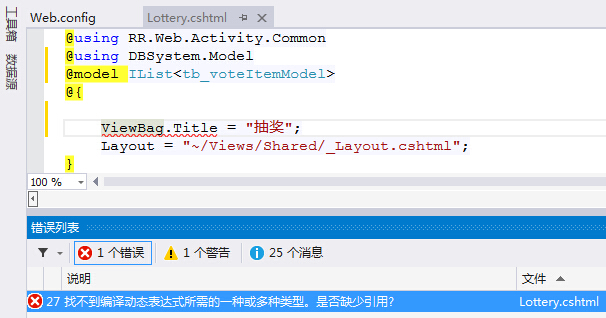
\includegraphics[scale=0.8]{MVCViewBagError.jpg}
	\caption{ViewBag错误}
	\label{fig:MVCViewBagError}
\end{figure}
	
首先查看是否已经引用Microsoft.CSharp.dll,
在配置文件的System.Web配置节中添加指定目标框架的相关配置,
如代码\ref{code:targetFrameworkConfig}所示。
因为ViewBag是.NET Framework 4.0中才有,
命名空间为System.Web.Mvc.dll。
由于compilation配置节中未指定targetFramework,
估计是程序默认为是比4.0的版本更低,
才出现此错误。

\begin{lstlisting}[language=XML,caption=配置MVC目标框架,label={code:targetFrameworkConfig}]
<system.web>
	<compilation debug="true" targetFramework="4.0" />
<system.web>
\end{lstlisting}

compilation配置节,
用于配置ASP.NET用于编译应用程序的所有编译设置。
targetFramework指定网站的目标.NET Framework的版本,
如果省略此特性,则目标版本将由Web.config文件中的其他设置以及与网站相关联的IIS应用程序池确定。
具体更多内容参见:\url{https://msdn.microsoft.com/zh-cn/library/vstudio/s10awwz0\%28v=VS.100\%29.aspx}。

\subsection{指定的转换无效}

在从接口接受到Object类型数据后,
需要转换为指定的泛型类型,提示指定的转换无效,
此时需要凡序列化返回的对象。

\begin{lstlisting}[language={[Sharp]C}]
/// <summary>
/// </summary>
/// <param name="relativeUrl">请求地址</param>
/// <param name="param">请求地址</param>
/// <returns></returns>
public static T SaveObject<T>(string relativeUrl, string param)
{
    var restUrl = PublicAttribute.WebApiPath + relativeUrl;
    var restResult = (Message) PublicAttribute.ApiClient.POST(restUrl, param);
    if (restResult == null)
        throw new RestfulNullDataException("接口返回空,url:" + restUrl + param);
    if (restResult.status)
    {
    	//不能直接强转为泛型T,需要反序列化
        return JsonConvert.DeserializeObject<T>(restResult.data.ToString());
    }
    PublicAttribute.Logger.Error("SaveObjects failed,url:" + restUrl + param + ",message:" + restResult.message);
    return default(T);
}
\end{lstlisting}

其中restResult.data为Object类型,使用JsonConvert反序列化为指定类型。

\subsection{未能加载文件或程序集“RR.Web.CCN.Tour”或它的某一个依赖项。试图加载格式不正确的程序。}

检查不能加载的程序集生成选项的目标平台是否是Any CPU,
在64位程序集直接加载单个的特殊的x86程序集会出现此错误。

\subsection{权限不足}

提示权限不足时,错误类似如下:CS0016: 未能写入输出文件,拒绝访问。
可以修改IIS应用程序池的标识,如图\ref{fig:ApplicationPoolIdentify}所示。

\begin{figure}[htbp]
	\centering
	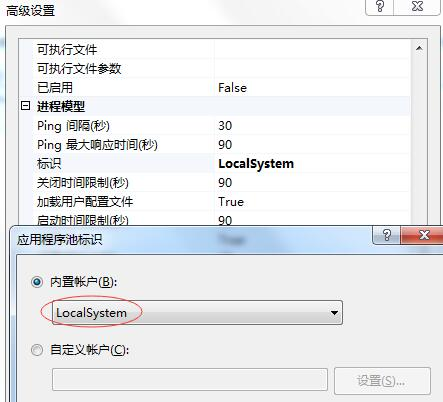
\includegraphics[scale=0.5]{ApplicationPoolIdentify.jpg}
	\caption{应用程序池权限}
	\label{fig:ApplicationPoolIdentify}
\end{figure}

\chapter{JavaScript}

\clearpage
\mbox{}         
\clearpage

JavaScript语句和JavaScript变量都对大小写敏感。
JavaScript的单线程,与它的用途有关。作为浏览器脚本语言,
JavaScript的主要用途是与用户互动,
以及操作DOM。这决定了它只能是单线程,
否则会带来很复杂的同步问题。比如,假定JavaScript同时有两个线程,
一个线程在某个DOM节点上添加内容,另一个线程删除了这个节点,
这时浏览器应该以哪个线程为准?
所以,为了避免复杂性,从一诞生,JavaScript就是单线程,
这已经成了这门语言的核心特征,将来也不会改变。
为了利用多核CPU的计算能力,HTML5提出Web Worker标准,
允许JavaScript脚本创建多个线程,但是子线程完全受主线程控制,
且不得操作DOM。所以,这个新标准并没有改变JavaScript单线程的本质。

\subsection{规范(Specification)}

\paragraph{表示区块起首的大括号,不要另起一行}

Javascript会自动添加句末的分号,导致一些难以察觉的错误。

\begin{enumerate}
\setcounter{enumi}{0}
\item{调用函数的时候,函数名与左括号之间没有空格}
\item{函数名与参数序列之间,没有空格}
\item{所有其他语法元素与左括号之间,都有一个空格}
\item{不要省略句末的分号}
\item{不要使用with语句}
\item{不要使用"相等"(==)运算符,只使用"严格相等"(===)运算符,
JS数据类型分为6类:Undefined Null String Number Boolean Object。
Javascript有两个表示"相等"的运算符:"相等"(==)和"严格相等"(===)。
因为"相等"运算符会自动转换变量类型,造成很多意想不到的情况,
建议使用严格相等}
\item{不要将不同目的的语句,合并成一行}
\item{所有变量声明都放在函数的头部}
\item{不要使用new命令,改用Object.create()命令}
这种做法的问题是,一旦你忘了加上new,myObject()内部的this关键字就会指向全局对象,
导致所有绑定在this上面的变量,都变成全部变量。
\item{建构函数的函数名,采用首字母大写(InitialCap);其他函数名,一律首字母小写}
\item{不要使用自增(++)和自减(--)运算符,用+=和-=代替}
\item{总是使用大括号表示区块}
\end{enumerate}

\subsection{进入页面时执行JavaScript}

两种方法实现在HTML页面加载完毕后运行某个JavaScript脚本。

\begin{lstlisting}[language=VBSCript]
<script type="text/javascript">
	/*JavaScript原生写法*/    
    window.onload = function () {
        //Run code when page load...
    }
    
    /*jQuery写法*/
    $(window).load = function () {
    	//Run code when page load...
    }
</script>
\end{lstlisting}

当一个文档完全下载到浏览器中时,
才会触发window.onload事件。
这意味着页面上的全部元素对JavaScript而言都是可以操作的,
也就是说页面上的所有元素加载完毕才会执行。
window对象是JavaScript层级中的顶层对象。
window对象会在<body>或<frameset>每次出现时被自动创建。
window对象表示一个浏览器窗口或一个框架。
在客户端JavaScript中,window 对象是全局对象,
所有的表达式都在当前的环境中计算。也就是说,
要引用当前窗口根本不需要特殊的语法,可以把那个窗口的属性作为全局变量来使用。
例如,可以只写 document,而不必写 window.document。
同样,可以把当前窗口对象的方法当作函数来使用,如只写 alert(),
而不必写 window.alert()。
除了上面列出的属性和方法,windos 对象还实现了核心 JavaScript 所定义的所有全局属性和方法。
window 对象的 window 属性和 self 属性引用的都是它自己。
当你想明确地引用当前窗口,而不仅仅是隐式地引用它时,
可以使用这两个属性。除了这两个属性之外,
parent 属性、top 属性以及 frame[] 数组都引用了与当前 window 对象相关的其他 window 对象。
以下为jQuery方法,需要引用jQuery文件。 

\begin{lstlisting}[language=VBSCript]
<script type="text/javascript">
	$(document).ready(function(){ 
	//Run code when page load...
}); 
</script> 
\end{lstlisting}

会在DOM完全就绪并可以使用时调用。
虽然这也意味着所有元素对脚本而言都是可以访问的,
但是,并不意味着所有关联的文件都已经下载完毕。
换句话说,当HMTL下载完成并解析为DOM树之后,代码就会执行。

\subsection{一道Javascript试题}


\begin{lstlisting}[language=VBScript]
function Foo() {
    getName = function () { alert (1); };
    return this;
}
Foo.getName = function () { alert (2);};
Foo.prototype.getName = function () { alert (3);};
var getName = function () { alert (4);};
function getName() { alert (5);}

//请写出以下输出结果:
Foo.getName();//2
getName();//4
Foo().getName();//1
getName();//1
new Foo.getName();//2
new Foo().getName();//3
new new Foo().getName();//3
\end{lstlisting}

第一问的Foo.getName是访问Foo函数上存储的静态属性。
第二问,直接调用 getName 函数。
既然是直接调用那么就是访问当前上文作用域内的叫getName的函数,
所以跟1 2 3都没什么关系。此题有无数面试者回答为5。
此处有两个坑,一是变量声明提升,二是函数表达式。

\paragraph{变量声明提升}所有声明变量或声明函数都会被提升到当前函数的顶部。

\paragraph{函数表达式}var getName与function getName都是声明语句,
区别在于var getName是函数表达式,而function getName是函数声明。

\subsection{Javascript日期}

Javascript的Date对象用于处理日期和时间,
如下代码片段。

\begin{lstlisting}[language=VBScript]
var myDate=new Date();
\end{lstlisting}

Date对象会自动把当前日期和时间保存为其初始值。

\subsection{jQuery Rotate插件实现旋转}

\begin{lstlisting}[language=VBScript]
var rotateFn = function (awards, angles, txt) {
    $('\#rotate').stopRotate();
    $('\#rotate').rotate({
        angle: 0,//起始角度
        animateTo: angles + 1800,//结束的角度
        duration: 8000,//转动时间
        callback: function () {
           //回调函数
        }
    });
};
\end{lstlisting}

\subsection{JavaScript调试}

\url{http://www.ruanyifeng.com/blog/2011/03/firebug_console_tutorial.html}

\subsection{匹配手机号码}

\begin{lstlisting}[language=VBSCript]
if (!userphone.match(/^1[3|4|5|8][0-9]\d{4,8}$/)) {
    tanc4_show("请输入正确的手机号码!"); return;
}
\end{lstlisting}

\subsection{JavaScript清空数组}

\subsubsection{splice}

\begin{lstlisting}[language=VBScript]
var ary = [1,2,3,4];
ary.splice(0,ary.length);
console.log(ary); // 输出 [],空数组,即被清空了
\end{lstlisting}

splice()方法可删除从index处开始的零个或多个元素,
并且用参数列表中声明的一个或多个值来替换那些被删除的元素。
第一个参数为起始位置,第二个参数为删除指定长度元素。
返回值是一个由所移除的元素组成的新Array对象。

\subsubsection{length赋值为0}

\begin{lstlisting}[language=VBScript]
var ary = [1,2,3,4];
ary.length = 0;
console.log(ary); // 输出 [],空数组,即被清空了
\end{lstlisting}


\subsubsection{赋值为[]}

\begin{lstlisting}[language=VBScript]
var ary = [1,2,3,4];
ary = []; // 赋值为一个空数组以达到清空原数组
\end{lstlisting}

这里其实并不能说是严格意义的清空数组,
只是将ary重新赋值为空数组,
之前的数组如果没有引用在指向它将等待垃圾回收。
length赋值为0保留了数组其它属性,赋值为[]则未保留。
很多人认为length赋值为0的效率很高些,
因为仅仅是给length重新赋值了,而方式3则重新建立个对象。
经测试恰恰是赋值为[]的效率高。

\subsection{数组是否有包含关系}

判断两个数组之间是否有包含关系,
mutexArr代表具有互斥元素的数组,
checkedArr代表当前选择的元素构成的数组,
要求选择的元素不能包含互斥元素。

\begin{lstlisting}[language=VBScript]
function contains1(mutexArr, checkedArr) {
    var i = mutexArr.length;
    var k = 0;
    while (i > 0) {
        var existsValue = $.inArray(mutexArr[i - 1], checkedArr);
        if (existsValue != -1) {
            k++;
        }
        i--;
    }
    if ((k == mutexArr.length || k > mutexArr.length) && k > 1) {
        return true;
    }
    return false;
}
\end{lstlisting}

需要使用jQuery元素是否包含在数组中的方法inArray,
inArray方法确定第一个参数在数组中的位置,
从0开始计数(如果没有找到则返回 -1 )。
也可以使用库函数Underscore.js\footnote{项目主页:http://underscorejs.org/。
Underscore provides over 100 functions that support both your favorite workaday functional helpers: 
map, filter, invoke — as well as more specialized goodies: function binding, 
javascript templating, creating quick indexes, 
deep equality testing, and so on. }中的intersection方法,
如代码所示。

\begin{lstlisting}[language=VBScript]
function contains2(mutexArr, checkedArr) {        
    var arr = _.intersection(mutexArr, checkedArr);
    if (arr.length > 1) {
        return true;
    }
    return false;
}
\end{lstlisting}

\_.intersection(*arrays)返回传入 arrays(数组)交集。
结果中的每个值是存在于传入的每个arrays(数组)里。

\subsection{XMLHttpRequest}

\subsection{获取元素文本}

以span元素为例,获取元素文本(此处是aaaa)可使用如下方式。

\begin{lstlisting}[language=HTML]
<span id="testid">aaaa</span>

/*方式1:从起始位置到终止位置的内容, 但它去除Html标签*/ 
var x1 = document.getElementById("testid").innerText;

/*方式2:从对象的起始位置到终止位置的全部内容,包括Html标签*/
var x2 = document.getElementById("testid").innerHTML;

/*jQuery写法*/ 
var x3 = $("#testid").text();
var x4 = $("#testid").val();
\end{lstlisting}

innerHTML会包含HTML页面中的换行符等,如果标签写法如下

\begin{lstlisting}[language=HTML]
<div id="demo">
<div>
\end{lstlisting}

那么通过document.getElementById("demo").innerHTML取出的内容其长度为1。
In Javascript, new lines are represented by a single "\textbackslash n" character.
Textarea values might have the character combos "\textbackslash n \textbackslash r" in the text box, but once they are pulled into Javascript,
 "\textbackslash n \textbackslash r" becomes JUST "\textbackslash n".
When replacing out new line characters, treat them as you would any other character. 
They are not special, they just have special notation.

\begin{lstlisting}[language=VBScript]
//用中文分号替换英文分号、中英文逗号或者回车
function ReplaceSeperator(mobiles) {
    var i;
    var result = "";
    var c;
    for (i = 0; i < mobiles.length; i++) {
        c = mobiles.substr(i, 1);
        if (c == ";" || c == "," || c == "," || c == "\n")
            result = result + ";";
        else if (c != "\r")
            result = result + c;
    }
    return result;
}
\end{lstlisting}

\subsection{序列化(Serialize)与反序列化(Deserialize)}

在针对参数较多的使用场景中,
将参数序列化为Json可以大大简化代码的编写和逻辑的处理。
JSON (JavaScript Object Notation) is a lightweight data-interchange format. 
It is easy for humans to read and write. It is easy for machines to parse and generate. 
It is based on a subset of the JavaScript Programming Language, 
Standard ECMA-262 3rd Edition - December 1999.
Douglas Crockford是Web开发领域最知名的技术权威之一,
ECMA JavaScript 2.0标准化委员会委员。
被JavaScript之父Brendan Eich称为JavaScript的大宗师(Yoda),
是JSON、JSLint、JSMin和ADSafe的创造者。

在数据传输流程中,Json是以文本,即字符串的形式传递的,
而JS操作的是JSON对象,所以,JSON对象和JSON字符串之间的相互转换是关键,
如下代码片段由Json字符串转化为Json对象。

\begin{lstlisting}[language=VBScript]
var str1 = '{ "name": "cxh", "sex": "man" }';
var obj = eval('(' + str1 + ')');
alert("eval:"+obj.name);
\end{lstlisting}

eval()函数是js自带的,
JavaScript原生的写法反序列化Json为对象,会产生安全和性能问题,不推荐使用.
IE8(兼容模式),IE7和IE6也可以使用eval()将字符串转为JSON对象,
但不推荐这些方式,这种方式不安全eval会执行json串中的表达式。 

\begin{lstlisting}[language=VBScript]
var str1 = '{ "name": "cxh", "sex": "man" }';

/*
由JSON字符串转换为JSON对象,使用jQuery封装的方法
*/
var objParseJson = jQuery.parseJSON(str1);
alert("objParseJson:" + objParseJson.name);

/*
由JSON字符串转换为JSON对象
*/
var objJsonParse = JSON.parse(str1);
alert("objJsonParse:" + objJsonParse.name);

/*
将对象转化为Json,IE7和IE6没有JSON对象
*/
var jsonParam = JSON.stringify(order);
\end{lstlisting}

\section{Ajax}

\subsection{Ajax提交原生写法}

Ajax的基础是XMLHttpRequest,XMLHttpRequest是一个浏览器接口,
使得Javascript可以进行HTTP(S)通信。

\begin{lstlisting}[language=VBScript]
function saveUserPhone(mobile) {
    var xhr = new XMLHttpRequest();
    xhr.onreadystatechange = function () {
        if (xhr.readyState === 4) {
            if (xhr.status === 200) {
            	var response=xhr.responseText;                
            } else {
            	xhr.abort();
                alert("服务器忙,请稍后重试");                
            }
        }
    }
    xhr.open("GET", "/Active/SaveUserPhone?phone=" + mobile, true);
    xhr.send(null);
}
\end{lstlisting}

最后一个参数asynch表示是否采用异步方法,true为异步,false为同步。

\subsection{Ajax提交}

Ajax提交的语法如下:

\begin{lstlisting}[language=VBScript]
$.post(url, { id: productId }, function (msg) {
    if (msg!== "OK") {
        alert("访问人数太多,请稍后再试!");
    }
});
\end{lstlisting}


\subsection{Ajax原理和XmlHttpRequest对象}

Ajax的原理简单来说通过XmlHttpRequest对象来向服务器发异步请求,从服务器获得数据,
然后用javascript来操作DOM而更新页面。
这其中最关键的一步就是从服务器获得请求数据。要清楚这个过程和原理,
我们必须对XMLHttpRequest有所了解。

XMLHttpRequest是ajax的核心机制,它是在IE5中首先引入的,是一种支持异步请求的技术。
简单的说,也就是javascript可以及时向服务器提出请求和处理响应,而不阻塞用户。达到无刷新的效果。
所以我们先从XMLHttpRequest讲起,来看看它的工作原理。
首先,我们先来看看XMLHttpRequest这个对象的属性。
它的属性有:

onreadystatechange  每次状态改变所触发事件的事件处理程序。

responseText     从服务器进程返回数据的字符串形式。

responseXML    从服务器进程返回的DOM兼容的文档数据对象。

status           从服务器返回的数字代码,比如常见的404(未找到)和200(已就绪)

status Text       伴随状态码的字符串信息

readyState       对象状态值

0 (未初始化) 对象已建立,但是尚未初始化(尚未调用open方法)

1 (初始化) 对象已建立,尚未调用send方法

2 (发送数据) send方法已调用,但是当前的状态及http头未知

3 (数据传送中) 已接收部分数据,因为响应及http头不全,这时通过responseBody和responseText获取部分数据会出现错误,

4 (完成) 数据接收完毕,此时可以通过通过responseXml和responseText获取完整的回应数据

但是,由于各浏览器之间存在差异,所以创建一个XMLHttpRequest对象可能需要不同的方法。
这个差异主要体现在IE和其它浏览器之间。下面是一个比较标准的创建XMLHttpRequest对象的方法。

\begin{lstlisting}[language=VBScript]
function CreateXmlHttp()
{
	//非IE浏览器创建XmlHttpRequest对象
	if(window.XmlHttpRequest)
	{
		xmlhttp=new XmlHttpRequest();
	}
	//IE浏览器创建XmlHttpRequest对象
	if(window.ActiveXObject)
	{
		try
		{
			xmlhttp=new ActiveXObject("Microsoft.XMLHTTP");  
		}
		catch(e)
		{
			try{
			 	xmlhttp=new ActiveXObject("msxml2.XMLHTTP");
			}
			catch(ex){
			}
		}
	}
}  
\end{lstlisting}

\section{jQuery}

jQuery的基本设计思想和主要用法,
就是“选择某个网页元素,然后对其进行某种操作”。
这是它区别于其他Javascript库的根本特点。
使用jQuery的第一步,往往就是将一个选择表达式,
放进构造函数jQuery()(简写为\$),
然后得到被选中的元素\footnote{http://www.ruanyifeng.com/blog/2011/07/jquery\_fundamentals.html}。
jQuery具有如下优势:

\begin{enumerate}
\setcounter{enumi}{0}
\item{轻量级}
\item{强大的选择器}
\item{出色的DOM操作封装}
\item{可靠的事件处理机制}
\item{完善的Ajax}
\item{不污染顶级变量}
\item{出色的浏览器兼容性}
\item{链式操作方式}
\item{隐式迭代,大幅减少代码量,减少循环结构}
\item{丰富的插件支持}
\item{行为层与结构层分离,是jQuery开发HTML开发各司其职}
\item{完善的文档}
\item{开源}
\end{enumerate}

\subsection{jQuery事件绑定}

jQuery事件绑定的3种写法:

\begin{lstlisting}[language=VBScript]
$("#apply").click(function(){});
$("#apply").bind("click",function(){});
$("body").on("click","#apply",function(){});
\end{lstlisting}

第一种写法只是bind方式的一种简写,
bind的第一个参数代表的含义是:事件类型(注意不需要加on),
function中的代码就是你要执行的逻辑代码。
bind还允许你绑定多个事件,事件名字之间用空格隔开。

\begin{lstlisting}[language=VBScript]
$("a").bind("click mouseover",function(){});
\end{lstlisting}

不管你用的是(click/bind/delegate)之中那个方法,
最终都是jQuery底层都是调用on方法来完成最终的事件绑定。
因此从某种角度来讲除了在书写的方便程度及习惯上挑选,
不如直接都采用on方法来的痛快和直接。
采用最简单写法容易产生过多绑定事件,
比较消耗内存。.bind(), .live(), .delegate()都是通过.on()来实现的,
.unbind(), .die(), .undelegate(),也是一样的都是通过.off()来实现的。
on方法的语法为:

\begin{lstlisting}[language=VBScript]
// jQuery 1.7+
$("ancestor").on( "click", "selector" [, data ], handler );
\end{lstlisting}

第一个参数是事件名称,第二个参数是子选择器,
从jQuery 1.7开始,on()函数提供了绑定事件处理程序所需的所有功能,
用于统一取代以前的bind()、 delegate()、 live()等事件函数。

\subsection{\$(function () \{\}) 的作用}

\$(function () \{\})其实是\$(document).ready()\{\})函数的缩写形式。
在\$(document).ready()\{\})函数内的所有代码都将在DOM加载完毕后,
页面全部内容(包括图片等)加载完毕前被执行。
在jQuery文件里面有定义\$=jQuery;用\$("\#id")和用jQuery("\#id")是一样的。
只是\$在其它的js框架里面也被用过,可能出现重复。

\begin{lstlisting}[language=VBScript]
var Hello = jQuery.noConflict();
\end{lstlisting}

这样以后就可以用Hello做前缀了

\begin{lstlisting}[language=VBScript]
Hello("txt1");
\end{lstlisting}

以下三种方式相同:

\begin{lstlisting}[language=VBScript]
$(document).ready(function() {  
   'Handler for .ready() called' 
});  
\end{lstlisting}

这个方法接收一个function类型的参数ready(handler), 
方法的作用是: Specify a function to execute when the DOM is fully loaded.
即当DOM加载完毕的时候,执行这个指定的方法.
因为只有document的状态ready之后,对page的操作才是安全的.
\$(document).ready()仅在DOM准备好的时候执行一次.
与之相比,load事件会等到页面渲染完成执行,
即等到所有的资源(比如图片)都完全加载完成的时候.
\$(window).load(function(){})\footnote{jQuery的写法,
JavaScript原生的写法如:window.onload=function()\{code goes on here...\}。
详情可参见:http://www.30t.com/index-htm-LangType-cn-BasePage-702-article\_id-6480.htm}会等整个页面,
不仅仅是DOM,还包括图像和iframes都准备好之后,再执行.
而ready()是在DOM准备好之后就执行了,
即DOM树建立完成的时候.所以通常ready()是一个更好的时机.

\begin{lstlisting}[language=VBScript]
$(function() {  
     'Handler for .ready() called'  
}); 
\end{lstlisting}

\begin{lstlisting}[language=VBScript]
$().ready(handler)
\end{lstlisting}


\subsection{CheckBox}

获取页面中选中的CheckBox的ID值。

\begin{lstlisting}[language=VBScript]
var str = "";
$("input[name="wjdc"]:checked").each(function () {
    str += $(this).attr("id") + ",";
});
alert(str);
\end{lstlisting}

this是JavaScript语言的一个关键字,
它代表函数运行时,自动生成的一个内部对象。
input标签下名称为wjdc且类型为CheckBox的ID值。
设置checkbox选中状态。

\begin{lstlisting}[language=VBScript]
$("#item_2-3").attr("checked", false);
\end{lstlisting}

其中\#item\_2-3为控件id,
在赋值控件名称时需要考虑jQuery特殊字符,
因为jQuery选择器是用正则表达式实现的,
所以正则表达式的特殊符号一般都要处理,
文档里面描述:使用如下任何的元字符

\begin{lstlisting}
!"#$%&'()*+,./:;<=>?@[\]^`{|}~
\end{lstlisting}

作为名称的文本部分时, 
它必须被两个反斜杠转义。

\subsection{jQuery中prop与attr区别}

在jQuery 1.6之前,只有attr()函数可用,
该函数不仅承担了attribute的设置和获取工作,
还同时承担了property的设置和获取工作。
例如:在jQuery 1.6之前,attr()也可以设置或获取tagName、className、nodeName、nodeType等DOM元素的property。

直到jQuery 1.6新增prop()函数,并用来承担property的设置或获取工作之后,
attr()才只用来负责attribute的设置和获取工作。

此外,对于表单元素的"checked"、"selected"、"disabled"等属性,
在jQuery 1.6之前,attr()获取这些属性的返回值为Boolean类型:如果被选中(或禁用)就返回true,否则返回false。

但是从1.6开始,使用attr()获取这些属性的返回值为String类型,
如果被选中(或禁用)就返回"checked"、"selected"或"disabled",
否则(即元素节点没有该属性)返回undefined。并且,在某些版本中,
这些属性值表示文档加载时的初始状态值,即使之后更改了这些元素的选中(或禁用)状态,
对应的属性值也不会发生改变。

因为jQuery认为:attribute的"checked"、"selected"、"disabled"就是表示该属性初始状态的值,
property的checked、selected、disabled才表示该属性实时状态的值(值为true或false)。

因此,在jQuery 1.6及以后版本中,
请使用prop()函数来设置或获取checked、selected、disabled等属性。对于其它能够用prop()实现的操作,
也尽量使用prop()函数。

\subsection{NETWORK\_ERR: XMLHttpRequest Exception 101}

Request aborted because it was cached or previously requested。
将aJax请求设置为异步即可。

\begin{lstlisting}[language=VBScript]
$.ajax({
	type: "get",
	data: { "userId": userId, "wxmediaId": res.serverId, "activityId": activityId },
	dataType: "json",
	cache: false,
	async: true,
	url: "/QiuJiFangJiaoHui/UpLoadImg?sjm=" + timestamp,
	success: function (data) {
		alert("上传成功");
		//设置上传状态,避免反复上传图片(如用户点击后退按钮返回到此页面)
		$("#IsUploaded").val("1");
		//跳转到特殊抽奖页面
		var webpath = $("#webpath").val();
		var url = webpath + "QiuJiFangJiaoHui/lotterySpecial?activityId=" + activityId;;
		window.location = url;
	},
	error: function (XMLHttpRequest, textStatus, errorThrown) {
		alert("errorThrown:" + errorThrown);
	}
});
\end{lstlisting}

\subsection{Ajax失效的}

ajax请求是同步还是异步造成的问题。
有时候我们会遇到这种情况,ajax请求方法,
里面配置和传值等等都是正确的,但是就是请求不到想要的数据,
到最后甚至怀疑是不是开发工具的问题,这时候你就应该观察一下,
ajax请求是异步还是同步。例如,你用post请求传值到另一个页面后台,
但是页面一加载你的ajax就已经执行过了,传值接收是在后台才完成的,
这时候就请求不到数据,所以可以考虑把ajax请求改为同步试试,
Ajax默认为异步。

\begin{quote}
By default, all requests are sent asynchronous (e.g. this is set to true by default). 
If you need synchronous requests, set this option to false. 
Note that synchronous requests may temporarily lock the browser, 
disabling any actions while the request is active.
\end{quote}


\chapter{HTML}


\subsection{规范}

\begin{itemize}
\item{用两个空格来代替制表符(tab) -- 这是唯一能保证在所有环境下获得一致展现的方法}
\item{嵌套元素应当缩进一次(即两个空格)}
\item{对于属性的定义,确保全部使用双引号,绝不要使用单引号}
\item{不要在自闭合(self-closing)元素的尾部添加斜线 -- HTML5 规范中明确说明这是可选的}
\item{不要省略可选的结束标签(closing tag)(例如,</li> 或 </body>)}
\item{建议为html根元素指定lang属性,从而为文档设置正确的语言。
这将有助于语音合成工具确定其所应该采用的发音,
有助于翻译工具确定其翻译时所应遵守的规则等等。}

\begin{lstlisting}[language=HTML]
<html lang="zh-CN">
  <!-- ... -->
</html>
\end{lstlisting}

\item{根据HTML5规范,在引入CSS和JavaScript文件时一般不需要指定type属性,
因为text/css和text/javascript分别是它们的默认值}

\item{http://codeguide.bootcss.com/}
\item{/是WebSite根目录,~/是ASP.NET Application根目录...}
\end{itemize}

\subsection{HTML5}

<!DOCTYPE>声明必须位于HTML5文档中的第一行,
也就是位于<html>标签之前。
该标签告知浏览器文档所使用的HTML规范。
doctype声明不属于HTML标签;tag;
它是一条指令,告诉浏览器编写页面所用的标记的版本。
在所有HTML文档中规定doctype是非常重要的,
这样浏览器就能了解预期的文档类型。
HTML 4.01中的doctype需要对DTD进行引用,
因为HTML 4.01基于SGML。而HTML 5不基于SGML,
因此不需要对DTD进行引用,但是需要doctype来规范浏览器的行为(让浏览器按照它们应该的方式来运行。)。
没有定义doctype才会开启怪异模式(Quirks Mode),
也就是说你只需要定义<!doctype html>就可以让浏览器在严格模式(标准模式)下渲染页面,
而不需要指定某个类型dtd。让我们来回顾一下,所有的浏览器都需要两种模式:
怪异模式和严格模式(Strict Mode)或者叫标准模式(Standards Mode)。
IE 6 for Windows/mac, Mozilla,Safari和Opera都实现了这两种模式,
但是IE 6以下版本永远定在了怪异模式。关于两种模式,你需要知道以下几点:

\begin{itemize}
\item{在标准化之前写的页面是没有doctype的,因此没有doctype的页面是在怪异模式下渲染的。}
\item{反过来说,如果web开发人员加入的doctype,说明他知道他所要做的事情,
大部分的doctype会开启严格模式(标准模式),页面也会按照标准来渲染。}
\item{任何新的或者未知的doctype都会开启严格模式(标准模式)。
每个浏览器都有自己的方式来激活怪异模式。你可以看看这个清单:http://hsivonen.iki.fi/doctype/}
\end{itemize}

\section{a标签}

\subsection{href="\#"}

通常情况下应该避免使用href="\#",
它会导致点击任何地方的时候页面自动移动到顶部。
You should (almost) never have href="\#". 
It is a link to an undefined anchor (which will be the top of the page). 
People who use it normally do so because they want to dangle JavaScript off it.
\#包含了一个位置信息,默认的锚是\#top也就是网页的上端,
所以出现了点击链接时网页自动定位到顶端的现象,
为了防止将页面定位到顶部,可以换一种写法:

\begin{lstlisting}[language=HTML]
<a href="javascript:void(0);" target="_blank"></a>
<a href="####"></a>
<a href="javascript:void(null)"></a>
\end{lstlisting}

void是一个操作符,这个操作符指定要计算一个表达式但是不返回值。
如果在void中写入0(void(0)),则什么也不执行,从而也就形成了一个空链接。
target为blank表示点击这个链接时跳转到一个空的页面。
\subsection{Meta}

META(Metadata)元素通常用于指定网页的描述,关键词,的文件的最后修改,作者,和其他元数据。
元数据可以被使用浏览器(如何显示内容或重新加载页面),搜索引擎(关键词),或其他 Web 服务调用。

\begin{lstlisting}[language=HTML]
<meta http-equiv="Content-Type" content="text/html; charset=utf-8" />
<meta charset="utf-8" />
\end{lstlisting}

charset属性是HTML5中的新属性,
且替换了:<meta http-equiv="Content-Type" content="text/html; charset=UTF-8">。
仍然允许使用http-equiv属性来规定字符集,但是使用新方法可以减少代码量。
http-equiv为HTTP响应的标题头Http Response Header)。

\begin{lstlisting}[language=HTML]
<meta name="参数" content="具体的参数值"/>
<meta http-equiv="参数" content="参数变量值"/>
\end{lstlisting}

\chapter{CSS}

\section{规范}

\subsubsection{文件规范}

1、文件均归档至约定的目录中。
具体要求通过豆瓣的CSS规范进行讲解:
所有的CSS分为两大类:通用类和业务类。通用的CSS文件,放在如下目录中:

\begin{itemize}
\item{基本样式库 /css/core}
\item{通用UI元素样式库 /css/lib}
\item{JS组件相关样式库 /css/ui}
\end{itemize}


业务类的CSS是指和具体产品相关的文件,放在如下目录中:
\begin{itemize}
\item{读书 /css/book/}
\item{电影 /css/movie/}
\item{音乐 /css/music/}
\item{社区 /css/sns/}
\item{小站 /css/site/}
\item{同城 /css/location/}
\item{电台 /css/radio/}
\end{itemize}

外联CSS文件适用于全站级和产品级通用的大文件。
内联CSS文件适用于在一个或几个页面共用的CSS。
另外一对具体的CSS进行文档化的整理。如:

\begin{itemize}
\item{util-01 reset /css/core/reset.css}
\item{util-02 通用模块容器 /css/core/mod.css}
\item{ui-01. 喜欢按钮 /css/core/fav\_btn.css}
\item{ui-02. 视频/相册列表项 /css/core/media\_item.css}
\item{ui-03. 评星 /css/core/rating.css}
\item{ui-04. 通用按钮 /css/core/common\_button.css}
\item{ui-05. 分页 /css/core/pagination.css}
\item{ui-06. 推荐按钮 /css/core/rec\_btn.css}
\item{ui-07. 老版对话框 /css/core/old\_dialog.css}
\item{ui-08. 老版Tab /css/core/old\_tab.css}
\item{ui-09. 老版成员列表 /css/core/old\_userlist.css}
\item{ui-10. 老版信息区 /css/core/notify.css}
\item{ui-11. 社区用户导航 /css/core/profile\_nav.css}
\item{ui-12. 当前大社区导航 /css/core/site\_nav.css}
\item{ui-13. 加载中 /css/lib/loading.css}
\end{itemize}

2、文件引入可通过外联或内联方式引入。
外联方式:(类型声明type=”text/css”可以省略)
内联方式: (类型声明type=”text/css”可以省略)
link和style标签都应该放入head中,原则上,
不允许在html上直接写样式。避免在CSS中使用@import,嵌套不要超过一层。

3、文件名、文件编码及文件大小
文件名必须由小写字母、数字、中划线组成
文件必须用UTF-8编码,使用UTF-8(非BOM),
在HTML中指定UTF-8编码,在CSS中则不需要特别指定因为默认就是UTF-8。
单个CSS文件避免过大(建议少于300行)

\subsubsection{命名规范}

\begin{itemize}
\item{规则命名中,一律采用小写加中划线的方式,不允许使用大写字母或\_}
\item{id用于标识模块或页面的某一个父容器区域,名称必须唯一,不要随意新建id}
\end{itemize}

\subsubsection{图片命名规范}

图片的名称分为头尾两部分,用下划线隔开,头部分表示此图片的大类性质
例如:广告、标志、菜单、按钮等等。
放置在页面顶部的广告、装饰图案等长方形的图片取名: banner
标志性的图片取名为: logo
在页面上位置不固定并且带有链接的小图片我们取名为 button
在页面上某一个位置连续出现,性质相同的链接栏目的图片我们取名: menu
装饰用的照片我们取名: pic
不带链接表示标题的图片我们取名: title
范例:banner\_sohu.gif  banner\_sina.gif  menu\_aboutus.gif  menu\_job.gif  title\_news.gif  logo\_police.gif   logo\_national.gif   pic\_people.jpg
鼠标感应效果图片命名规范为”图片名+\_+on/off”。
例如:menu1\_on.gif  menu1\_off.gif

\subsection{选择器优先级}

一般而言,选择器越特殊,它的优先级越高。
也就是选择器指向的越准确,它的优先级就越高。
通常我们用1表示标签名选择器的优先级,
用10表示类选择器的优先级,用100标示ID选择器的优先级,
内联样式表的权值为1000。一般不建议使用内联样式表,
也完全违背了内容和显示分离或结构与表现分离的思想,
DIV+CSS的优点也不能再有任何体现。
良好结构的HTML页面内几乎没有表现属性的标签。
代码非常干净简洁。例如,原先的代码,现在可以只在HTML中写,
所有控制表现的东西都写到CSS中去,在结构化的HTML中, 
table就是表格,而不是其他什么(更不能被用来布局和定位)。

\subsection{标签}

\begin{lstlisting}[caption=CSS代码标签示例,label={code:CSSLearingLabel}]
 .content{
     line-height: 35px;
     font-size: 25px;
     text-align: center;            
     font-family: Georgia,Serif`\makeremark{font-family 可以把多个字体名称作为一个“回退”系统来保存。如果浏览器不支持第一个字体,则会尝试下一个。也就是说,font-family 属性的值是用于某个元素的字体族名称或/及类族名称的一个优先表。浏览器会使用它可识别的第一个值。}`; 
     display: block`\makeremark{这个属性用于定义建立布局时元素生成的显示框类型。对于 HTML 等文档类型,如果使用 display 不谨慎会很危险,因为可能违反 HTML 中已经定义的显示层次结构。对于 XML,由于 XML 没有内置的这种层次结构,所有 display 是绝对必要的。值为block时此元素将显示为块级元素,此元素前后会带有换行符。}`;
     width: 600px;
     height: 400px;
     overflow: scroll`\makeremark{overflow属性规定当内容溢出元素框时发生的事情,如果值为scroll,不论是否需要,用户代理都会提供一种滚动机制。因此,有可能即使元素框中可以放下所有内容也会出现滚动条。}`;
     text-decoration: underline;
     border: 5px solid #e2d218`\makeremark{border-width border-style border-color}`;
     clear: both`\makeremark{clear 属性规定元素的哪一侧不允许其他浮动元素,both在左右两侧均不允许浮动元素。}`;          
 }
\end{lstlisting}

\showremarks

使用 max-width 替代 width 可以使浏览器更好地处理小窗口的情况。
这点在移动设备上显得尤为重要。
“响应式设计(Responsive Design)”是一种让网站针对不同的浏览器和设备“响应”不同显示效果的策略,
这样可以让网站在任何情况下显示的很棒! 


\subsection{水平居中}

\paragraph{把margin设为auto}

就是把要居中的元素的margin-left和margin-right都设为auto,
如下代码所示:

\begin{lstlisting}
margin:0 auto;
\end{lstlisting}

此方法只能进行水平的居中,且对浮动元素或绝对定位元素无效。
行级元素设置其父元素的text-align center,
块级元素设置其本身的left和right margins为auto即可。

\paragraph{使用text-align:center}

只能对图片,按钮,文字等行内元素(display为inline或inline-block等)进行水平居中。
但要说明的是在IE6、7这两个奇葩的浏览器中,它是能对任何元素进行水平居中的。

\paragraph{使用line-height让单行的文字垂直居中}

把文字的line-height设为文字父容器的高度,适用于只有一行文字的情况。

\subsection{宽高自适应}

在IE7+及chrome、firefox等浏览器中,
高度自适应可以利用绝对定位来解决。
但一个元素是绝对定位时,如果没有给它设定高度或宽度,
则它的的高度和宽度是由它的top、right、bottom、left属性决定的,
但这一法则在IE6中并不适用,因此在IE6中还得另辟蹊径。
在IE6中给html设定padding,并不会撑大html元素的尺寸,
这正是我们要利用的地方。


\begin{lstlisting}[language=HTML]
<style> 
    .headbanner {
        position: absolute;
        bottom: 0px;
        top: 0px;`\makeremark{bottom和top设置高度自适应}`
        left:0;
        roght:0;`\makeremark{left和right设置宽度自适应}`
        text-align: center;
        max-width: 720px;
    }   

    .headbanner img{
        width: 100%;
        height: 100%;`\makeremark{高度的计算方式完全不一样。事实上,浏览器根本就不计算内容的高度,除非内容超出了视窗范围(导致滚动条出现)。或者你给整个页面设置一个绝对高度。否则,浏览器就会简单的让内容往下堆砌,页面的高度根本就无需考虑。想让一个元素的百分比高度起作用,你需要给这个元素的至少一个父元素的高度设定一个有效值。百分比是指其相对父块高度而定义的高度,也就是按照离它最近且有定义高度的父层的高度来定义高度。}`        
    }    
</style>

<body> 
    <div class="headbanner">
        <img src="~/Resource/image/banner\_01.png">        
    </div>
</body>
\end{lstlisting}

\showremarks

\subsection{竖直居中}

先要设置div元素的祖先元素html和body的高度为100\%(因为他们默认是为0的),
并且清除默认样式,即把margin和padding设置为0(如果不清除默认样式的话,
浏览器就会出现滚动条)。竖着居中的CSS代码如下所示:

\begin{lstlisting}[language=HTML]
<!DOCTYPE html>
<html lang="en">
<head>
    <meta charset="UTF-8">
    <title>index</title>
    <style>
        html,body {
            width: 100%;
            height: 100%;
            margin: 0;
            padding: 0;
        }
        .content {
            width: 300px;
            height: 300px;
            background: orange;
            margin: 0 auto; /*水平居中*/
            position: relative; /*脱离文档流*/
            top: 50%; /*偏移*/
            margin-top: -150px;
        }
    </style>
</head>
<body>
    <div class="content"></div>
</body>
</html>
\end{lstlisting}


\subsection{CSS3 Media Queries}

\subsection{属性}

\subsubsection{display}

一个常用的display值是 none 。
一些特殊元素的默认 display 值是它,
例如script 。 display:none 通常被JavaScript用来在不删除元素的情况下隐藏或显示元素。
它和visibility属性不一样。把display设置成none不会保留元素本该显示的空间,
但是 visibility: hidden; 还会保留。 

\subsubsection{z-index}

用来确定定位元素在垂直于显示屏方向(以下称为Z轴)上的层叠顺序。
要想给元素设置z-index样式,必须先让它变成定位元素,
再通俗一点说,就是要给元素设置一个postion:relative(或者 absolute或者fixed)样式。
不要给想控制“上、下”的元素设置z-index,
而是对他们的父容器设置z-index样式。
这一点详细解释和原因在《精通html和css设计模式》一书中较为详细的解释。

每个box都归属于一个stacking context,
它是元素在z轴方向上定位的参考。根元素形成 root stacking context,
其他stacking context由定位元素设置z-index为非auto时产生。
如\#div1{position:relative;z-index:0;}即可使 id=div1的元素产生stacking context。
stacking context和 containing block 并没有必然联系。
在一个stacking context中的每个box,都有一个stack level(即层叠级别,以下统一用stack level),
它决定着在同一stacking context中每个box在z轴上的显示顺序。同一stacking context中,
stack level值大的显示在上,stack level值小的显示在下,
同一stack level的遵循后来居上的原则(back-to-front )。
不同stacking context中,
元素显示顺序以父级的stacking context的stack level来决定显示的先后情况。
于自身stack level无关。注意stack level和z-index并不是统一概念。

\subsubsection{rel}

rel是relationship的英文缩写,rel属性通常出现在a,link标签中,
在引用css时,rel不能省略,只有rel属性的"stylesheet"值得到了所有浏览器的支持,
其他值只得到了部分地支持。

\subsection{title}

W3C组织建议把所有网页上的对像都放 在一个盒(box)中,
设计师可以通过创建定义来控制这个盒的属性,
这些对像包括段落、列表、标题、图片以及层。盒模型主要定义四个区域:
内容 (content)、边框距(padding)、边界(border)和边距(margin)。
 对于初学者,经常会搞不清楚margin,background-color,
 background- image,padding,content,border之间的层次、关系和相互影响。
 这里提供一张盒模型的3D示意图,希望便于你的理解和记忆。

\subsection{css !important}

css !important作用是提高指定CSS样式规则的应用优先权。\section{AngularJS}

AngularJS是比较新的技术,版本1.0是在 2012 年发布的。
AngularJS是由Google的员工Miško Hevery从2009年开始着手开发。
这是一个非常好的构想,该项目目前已由Google正式支持,
有一个全职的开发团队继续开发和维护这个库。
AngularJS 是一个 JavaScript 框架。
它是一个以 JavaScript 编写的库。
AngularJS is an MVC framework for building web applications. 
The core features include HTML enhanced with custom 
component and data-binding capabilities, 
dependency injection and strong focus on simplicity, 
testability, maintainability and boiler-plate reduction.
百度开源静态链接:http://apps.bdimg.com/libs/angular.js/1.2.16/angular.min.js。

\section{线程}

\subsection{托管线程}

\section{扩展方法}





\chapter{数据库}

\section{SQLite}

\subsection{SQLite连接}

The System.Data.Common namespace provides 
classes for creating DbProviderFactory instances to work with specific data sources.
When you create a DbProviderFactory instance and 
pass it information about the data provider, 
the DbProviderFactory can determine the correct, 
strongly typed connection object to return based on the information it has been provided.

\begin{lstlisting}[language={[Sharp]C}]
public SqliteOperateHelper(DbProviderFactory factory, string connectionString)
{
    _dbConnection = factory.CreateConnection();
    if (_dbConnection == null) return;
    _dbConnection.ConnectionString = connectionString;
    var cnnstring = factory.CreateConnectionStringBuilder();
    if (cnnstring == null) return;
    cnnstring.ConnectionString = connectionString;
    _dbConnection.Open();
}
\end{lstlisting}

\section{数据恢复}

误删除了微信用户表中的数据。
查看数据库的备份历史。

\begin{lstlisting}[language=SQL]
SELECT  database_name,recovery_model,name,backup_start_date    
FROM msdb.dbo.backupset
order by backup_start_date desc
\end{lstlisting}

\paragraph{Step 1}~~将微信用户数据Pull到测试库中。
删除表中重复的记录。

\begin{lstlisting}[language=SQL]
/*删除tb_wxUser表中重复的记录(根据OpenID匹配)*/
delete from tb_wxUser
where openid in 
(
	select openid 
	from tb_wxUser 
	group by openid 
	having count(openid) > 1
)
and wxUserId not in 
(
	select top 1 wxUserId
	from tb_wxUser
	where openid =
	(
		select top 1 openid
		from tb_wxUser	 
		group by openid 
		having count(openid)>1		
	)
	order by wxUserId desc	
)
\end{lstlisting}

数据库的恢复模式设置为完整。

\section{数据库还原}

\subsection{切换到单用户还原}

在还原数据库时,有时会提示无法获取数据库的独占访问权,
是因为其他用户在还原的时刻连接数据库,
此时可将数据库设置为单用户模式。

\begin{lstlisting}[language=SQL]
--将数据库切换到单用户模式
alter database [zouwo-weixin] set single_user;

--将数据库切换到多用户模式
alter database [zouwo-weixin] set single_user;
\end{lstlisting}

\subsection{活动监视器}

也可以打开SQL Server的活动监视器终止当前连接的用户再进行还原,
此种方式比较暴力,不推荐此种方式。

\subsection{数据泵(Data Pump)}

SQL Server跨服务器不同数据库之间复制表的数据,
需要用到链接服务器。

\begin{quotation}
A linked server configuration enables SQL Server to 
execute commands against OLE DB data sources on remote servers. 
Linked servers offer the following advantages:

\begin{itemize}

\item{Remote server access.}

\item{The ability to issue distributed queries, updates, commands, and transactions on heterogeneous data sources across the enterprise.}

\item{The ability to address diverse data sources similarly.}

\end{itemize}

\end{quotation}

创建链接服务器可以通过2种方式。
创建链接服务器在服务器安全对象下的链接服务器,
右键创建链接服务器,链接服务器填写服务器IP,
非默认端口时填写端口。安全性选项卡中选择使用此上下文建立链接,
输入登录用户名密码。

\begin{lstlisting}[language=SQL]
--添加远程链接服务器
exec sp_addlinkedserver
	@server='LinkServer', --远程服务器别名
	@srvproduct='',
	@provider='SQLOLEDB',
	@datasrc='139.28.81.128,5002'
go

--添加远程登录
exec sp_addlinkedsrvlogin 'LinkServer','false',null,'数据库登录名','数据库登录密码'
go

--以后不再使用时删除链接服务器  
exec sp_dropserver 'LinkServer','droplogins'

--显示可用的服务器
exec sp_helpserver 
\end{lstlisting}

sp\_dropserver存储过程为不再使用时删除链接服务器,
往服务器上导入数据如下语句所示。

\begin{lstlisting}[language=SQL]
--将表1结构复制到表2
select *
into [renren-weixin].[dbo].[tb_wxUser1]
from [renren-weixin].[dbo].[tb_wxUser] 
where 1=0

--把本地表导入远程表,远程表必须已经存在,且远程表不应设置标识列或主键 
insert openquery ([129.21.80.128,5002], ' SELECT * FROM [renren-weixin].[dbo].[tb_wxUser1] ' ) 
select * from [zouwo-weixin].[dbo].tb_wxUser

--将远程表导入本地表
select * into tb_awardsCopy from openrowset('SQLOLEDB ', '129.21.80.128,5002'; 'renren-admin'; 'renren-admin!@#','select * from [renren-system].[dbo].[tb_awards]')

--用表2的记录更新表1(通过openid匹配,openid唯一)
update tb_wxUser
set tb_wxUser.subscribe_time=tb_wxUser1.subscribe_time
from tb_wxUser1
where tb_wxUser.openid=tb_wxUser1.openid
and tb_wxUser.accountId=1 

--根据最后一次关注时间更新微信用户表数据的添加时间
update tb_wxUser
set addDate =dateadd(s,cast(tb_wxUser.subscribe_time as bigint),'1970-01-01 00:00:00:000')
where addDate >'2015-09-17 15:09:09.000'
\end{lstlisting}

在将远程表导入本地表时,
数据库应该不存在相同表名的表。
将本地的tb\_wxUser表数据导入到远程服务器的tb\_wxUser1表中。
链接服务器如图\ref{fig:LinkServerTier}所示。

\begin{figure}[htbp]
	\centering
	\includegraphics[scale=0.8]{LinkServerTier.bmp}
	\caption{Link Servers}
	\label{fig:LinkServerTier}
\end{figure}

微信消息接口中的订阅时间(Subscribe Time)表示距离1970年的秒数。

\subsection{常用SQL}

\begin{lstlisting}[language=SQL]
--修改列的字段类型长度
alter table tb_question alter column  "question" nvarchar(50) null

--修改列名
exec sp_rename 'tb_question.[questionnaireType]', 'questionType', 'column'

--添加列

--数据表是否存在
if exists (
select * 
from sysobjects 
where id =object_id(N'[tb_surveyAnalysisDetail]'))
begin
	drop table dbo.tb_surveyAnalysisDetail
end

--数据列是否存在(当列名是整型时,需要手动转换为字符类型,在添加四个双引号与列名匹配)	
if not exists
(
	select * 
	from syscolumns 
	where id=object_id('tb_surveyAnalysisDetail') 
	and name=''''+Convert(nvarchar(256),@questionId)+''''
) 

--当运行是才知道列名时,动态指定列名
select @updateSql='update tb_surveyAnalysisDetail set '+@columnName+'='''+@answerContent+''' where userId=@userId'
exec sp_executesql @updateSql
					,N'@columnName nvarchar(256),@userId int'
					,@columnName=@columnName
					,@userId=@userid

--查询端口号
exec sys.sp_readerrorlog 0, 1, 'listening'

--将一个表(表结构+数据)复制到另一个表,跨库不跨IP
select * into [renren-tour].[dbo].tour_seller
from [RR-CCN].[dbo].discount_seller

--查询PV、UV
select count(distinct userId) as 'UV'`\makeremark{剔除掉重复的用户并统计出结果集的行数可用count(distinct 列名)的方式}`,
count(*) as PV
from discount_visitorLog
where siteType=3
and visitTime between '2015-11-10 00:00:00.000' and '2015-11-10 23:59:59.000'

--查看某一个数据库(zouwo-system)当前的连接数
select * 
from [master].[dbo].[sysprocesses] where [dbid] in 
(
  select [dbid]
  from [master].[dbo].[sysdatabases] 
  where name='zouwo-system'
)

--使数据库脱机(还原数据库时)
alter database [datebase] set offline with rollback immediate
\end{lstlisting}

\showremarks

Value of error log file you want to read: 0 = current, 1 = Archive \#1, 2 = Archive \#2, etc...
Log file type: 1 or NULL = error log, 2 = SQL Agent log
Search string 1: String one you want to search for
Search string 2: String two you want to search for to further refine the results

\subsection{函数(Function)}

\subsubsection{分割字符串}

\begin{lstlisting}[language=SQL]
ALTER FUNCTION [dbo].[SplitString]
(
	@Input NVARCHAR(MAX), --input string to be separated
	@Separator NVARCHAR(MAX)=',', --a string that delimit the substrings in the input string
	@RemoveEmptyEntries BIT=1 --the return value does not include array elements that contain an empty string
)
RETURNS @TABLE TABLE
(
	[Id] INT IDENTITY(1,1),
	[VALUE] NVARCHAR(MAX)
)
AS
BEGIN
	DECLARE @Index INT, @Entry NVARCHAR(MAX)
	SET @Index = CHARINDEX(@Separator,@Input)
	WHILE (@Index>0)
	BEGIN
		SET @Entry=LTRIM(RTRIM(SUBSTRING(@Input, 1, @Index-1)))
		IF (@RemoveEmptyEntries=0) OR (@RemoveEmptyEntries=1 AND @Entry<>'')
		BEGIN
			INSERT INTO @TABLE([VALUE]) VALUES(@Entry)
		END
		SET @Input = SUBSTRING(@Input, @Index+DATALENGTH(@Separator)/2, LEN(@Input))
		SET @Index = CHARINDEX(@Separator, @Input)
		END
		SET @Entry=LTRIM(RTRIM(@Input))
		
		IF (@RemoveEmptyEntries=0) OR (@RemoveEmptyEntries=1 AND @Entry<>'')
		BEGIN
			INSERT INTO @TABLE([VALUE]) VALUES(@Entry)
		END
	RETURN
END
\end{lstlisting}

\subsection{存储过程(Procedure)}

\section{mysql}

\subsection{常用查询}

\begin{lstlisting}[language=Bash]
mysql --host=localhost --user=readmine_admin --password=123
SET PASSWORD FOR 'root'@'localhost' = PASSWORD('newpass');

#To see which user you are, and whose permissions you have
select user(), current_user();
\end{lstlisting}



\section{定时任务}

工作中经常忘记提交代码,
可通过Windows自带的at命令设置定时任务,
比如每天下午的6点自动进行代码提交。
取消计划任务时,只需要用at命令查询出任务的ID,
根据ID取消即可,如果不带参数ID,
那么就是删除所有已知的任务。

\begin{lstlisting}[language=Bash]
#删除指定定时任务
at id /delete

#删除所有定时任务
at /delete
\end{lstlisting}

at命令虽然可以执行定时任务,
一直未尝试成功,可用schtasks命令替代。
schtasks命令每天运行的脚本如下:

\begin{lstlisting}[language=Bash]
#每天晚上的8:00定时关机
at 20:00 /every:M,T,W,Th,F,S,Su shutdown -f -s -t 60

#23:44:00定时运行脚本提交代码
schtasks /create /tn "Code Commit" /tr G:\CommitCode.bat /sc daily /st 23:44:00 /ed 2100/12/31

#每隔一分钟运行同步脚本,注意脚本的路径文件夹名称最好不要有空格,可能导致任务无法启动
schtasks /create /sc minute /mo 1 /tn "Sync log" /tr "D:\AutoSync.bat"

#定时提醒提交代码
schtasks /create /tn CodeCommit /sc daily /st 09:12:00 /tr "mshta vbscript:msgbox(\"记得提交代码!\",64,\"定时提醒\")(window.close)"

#查询schtasks建立的任务列表时需更改cmd的语言为英文(输入命令:chcp 437), 
执行查询计划任务命令(命令:schtasks /query)后再改回简体中文(输入命令:chcp 936)

schtasks /Query

chcp 437 `\makeremark{显示或设置活动代码页编号为英文(change code page)}`
schtasks /query /TN "auto update SVN" `\makeremark{查询出作业名称为“auto update SVN”的作业,TN代表Task Name}`
schtasks /delete /TN "auto update SVN" `\makeremark{移除作业名称为“auto update SVN”的作业}`
\end{lstlisting}

\showremarks

脚本的含义为每天晚上的23:44运行批处理脚本CommitCode.bat,
直到2100年12月31日为止,任务的名称为Code Commit。

\section{刷新页面}

1 history.go(0)

2 location.reload()

3 location=location

4 location.assign(location)

5 document.execCommand(‘Refresh‘)

6 window.navigate(location)

7 location.replace(location)

8 document.URL=location.href


\chapter{安全(Security)}

\clearpage
\mbox{}         
\clearpage

物理路径泄露,CGI源代码泄露,目录遍历,执行任意命令,缓冲区溢出,拒绝服务,SQL注入,条件竞争和跨站脚本执行漏洞。
首先需要说明的是,入侵者的来源有两种,
一种是内部人员利用自己的工作机会和权限来获取不应该获取的权限而进行的攻击。
另一种是外部人员入侵,包括远程入侵、网络节点接入入侵等。
进行网络攻击是一件系统性很强的工作,其主要工作流程是:
收集情报,远程攻击,远程登录,取得普通用户的权限,
取得超级用户的权限,留下后门,清除日志。
主要内容包括目标分析,文档获取,破解密码,日志清除等技术,
如图所示。

\begin{figure}[htbp]
	\centering
	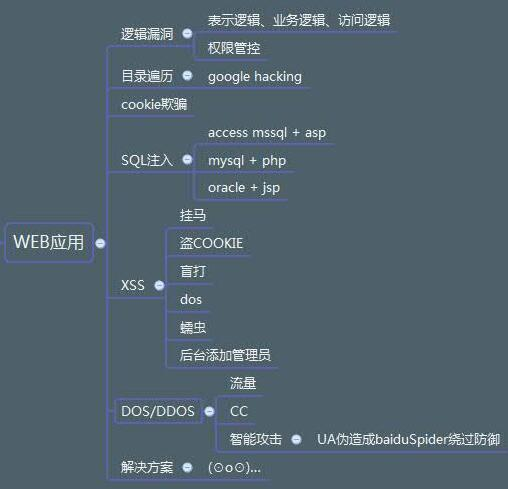
\includegraphics[scale=0.8]{NormalWebSecurity.jpg}
	\caption{常见Web攻击}
	\label{fig:NormalWebSecurity}
\end{figure}



\section{Encrypt Algorithms}

Hash,一般翻译做“散列”,也有直接音译为“哈希”的,就是把任意长度的输入(又叫做预映射, pre-image),
通过散列算法,变换成固定长度的输出,该输出就是散列值。这种转换是一种压缩映射,
也就是,散列值的空间通常远小于输入的空间,不同的输入可能会散列成相同的输出,
而不可能从散列值来唯一的确定输入值。简单的说就是一种将任意长度的消息压缩到某一固定长度的消息摘要的函数。

HASH主要用于信息安全领域中加密算法,它把一些不同长度的信息转化成杂乱的128位的编码,
这些编码值叫做HASH值。也可以说,hash就是找到一种数据内容和数据存放地址之间的映射关系。
常见的Hash算法有:MD4、MD5、SHA-1、HAVAL等。
HAVAL is a cryptographic hash function. 
Unlike MD5, but like most modern cryptographic hash functions, 
HAVAL can produce hashes of different lengths. 
HAVAL can produce hashes in lengths of 128 bits, 160 bits, 192 bits, 224 bits, and 256 bits. 
HAVAL also allows users to specify the number of rounds (3, 4, or 5) to be used to generate the hash.
HAVAL目前还没有C\#实现。

\subsection{网站登录安全(Website Login Security)}

博客园登录的用户名密码采用了JSEncrypt库进行RSA加密,
公钥通过OpenSSL生成后通过网页分发到客户端,
用户名和密码经过JSEncrypt加密后发送到服务器。
通过OpenSSL生成公钥和私钥对,生成公钥的命令如下:

\begin{lstlisting}[language=Bash]
openssl genrsa -out rsa_1024_priv.pem 1024
\end{lstlisting}

接下来根据公钥生成私钥,使用如下命令:

\begin{lstlisting}[language=Bash]
openssl rsa -pubout -in rsa_1024_priv.pem -out rsa_1024_pub.pem
\end{lstlisting}

私钥保存在服务器端,经过公钥加密后的数据通过私钥进行解密,
在与数据库的用户名密码进行比对。
注意在后端需要将OpenSSL生成的私钥转换为XML格式,再进行解密。
Javascript本身是经过明文加密,通过手段理论上可进行破解(研究中),
还有就是采用安全控件(淘宝),控件的作用就是用二进制代码来隐藏加密的算法,
防止密码在发送前被截获,
不知道算法,也就很难破解原文。在不使用原文的情况下,
使用密文来模拟用户的登录也是可以的,实际上单纯的加密也是无法满足要求的,
所以就有了盐值,相同的密码多次生成的结果完全不同,非随机盐也会被摸出规律。
所以就采用HTTPS对通讯进行加密,但是SSL也会爆出漏洞,病毒木马窥视内存同样存在,
所以优秀的算法尽量不将明文保存在内存中,或者尽量在内存中停留极短时间。
还有就是采用硬件加密,当然最安全的就是把电源和网线拔了,
把电脑拆成零件锁到保险柜里面。

\section{RESTful API认证}

所有的REST API调用必须运行在使用可信的CA签名过的证书的HTTPS之上。
所有客户端与服务端交互之间必须要验证服务端证书。
通过使用由可信机构签名的证书,SSL可以保护你免受“中间人”攻击。
中间人攻击的手段是在客户端和服务端之间插入一个代理进而窃听“加密的”通信。
如果你不验证服务端的SSL证书,你就无法知道谁在接收你的REST查询请求。

所有的REST API调用应该通过专门的API密钥完成,
该密钥由标识成分和共享密钥两部分组成。
系统必须允许一个指定客户端拥有多个活动的API密钥并能方便地让个别密钥失效。
前半部分的重点是发起REST请求的系统不应是某个交互用户……REST认证的的是程序而不是人,
它支持比人使用的用户名/密码更强大的认证手段。
后半部分的意思是,每个REST服务器应该支持每个客户端拥有多个API密钥。
该需求使得孤立潜在危害和当危害发生时解决问题更为简单。
当应用被破坏时,你也需要一种完善的方式铺开替换的API密钥。

所有的REST查询必须通过签名令牌签名的方式进行认证,
该过程通过对按小写的字母顺序排序的查询参数使用私钥进行签名。
签名应在查询字符串的URL编码前完成。
换言之,你不能将共享密钥作为查询串的一部分进行传递,
而应使用它进行签名。签名后的查询串看起来应该是这样的:

\begin{lstlisting}[language=HTML]
GET /object?timestamp=1261496500&apiKey=Qwerty2010&signature=abcdef0123456789
\end{lstlisting}
   
被签名的串是:

\begin{lstlisting}[language=HTML]
/object?apikey=Qwerty2010&timestamp=1261496500
\end{lstlisting}

而签名是应用API密钥的私钥所得到的HMAC-SHA256哈希值。

\subsection{Basic Authentication}

Basic Authentication需要和HTTPS一起使用,
Http Basic是一种比较简单的身份认证方式。
在Http header中添加键值对Authorization: Basic xxx (xxx 是 username:passowrd base64值)。
而Base64的解码是非常方便的,如果不使用HTTPS,相当于是帐号密码直接暴露在请求中。

\subsection{Api Key + Security Key + Sign}

\begin{enumerate}
	\setcounter{enumi}{0}
    \item{用户登录返回一个api\_key和security\_key}注意这里返回的两个key可以被劫持,所以为了进一步安全可以考虑下放key时采用非对称加密进行下放,服务端采用服务端的私钥进行签名,签名后用客户端的公钥进行加密,
客户端接收后用客户端的私钥进行解密,
服务端的公钥解密出发送的内容(key)。
    \item{然后客户端将security\_key存在客户端}
    \item{当要发送请求之前,通过function2加密方法,把如图所示的五个值一起加密,得到一个sign}
    \item{发送请求的时候,则将除去security\_key之外的值,以及sign一起发送给服务器端}
    \item{服务器端首先验证时间戳是否有效,比如是服务器时间戳5分钟之前的请求视为无效}
    \item{然后根据api\_key得到sercurity\_key}
    \item{最后验证sign}
\end{enumerate}

\subsection{Amazon的API鉴权流程}

\begin{enumerate}
\setcounter{enumi}{0}
\item{[客户端]在调用REST API之前,首先将待发送消息体打包,combine a bunch of unique data together (Web Sevice端将要接收的数据)}
\item{[客户端]用系统分派的密钥使用哈希(最好是HMAC\footnote{HMAC是密钥相关的哈希运算消息认证码(Hash-based Message Authentication Code),HMAC运算利用哈希算法,以一个密钥和一个消息为输入,生成一个消息摘要作为输出。}-SHA\footnote{哈希安全算法(Secure Hash Algorithm),确切地说,这不是一种算法,而是一组加密哈希函数,由美国国家标准技术研究所首先提出。无论是你的应用商店,电子邮件和杀毒软件,还是浏览器等等,都使用这种算法来保证你正常下载,以及是否被“中间人攻击”,或者“网络钓鱼”。}1 or SHA256)加密(第一步的数据)}
\item{[客户端]向服务器发送数据}
发送生成的HMAC码.

发送消息体(属性名和属性值),如果是私有信息需要加密,像是(“mode=start\&number=4\&order=desc”或其他不重要的信息)直接发送即可.

(可选项)避免重放攻击(Replay Attacks)的唯一办法就是加上时间戳。
在使用HMAC(Hash-based Message Authentication Code)算法时加入时间戳,
这样系统就能依据一定的条件去验证是否有重放的请求并拒绝.

用户身份认证信息例如,用户ID,客户ID或是其他能别用户身份的信息。这是公共API,大家都能访问的到(自然也包括了那些居心叵测的访问者)系统仅仅需要这部分信息来区分发信人而不考虑可靠与否(当然可以通过HMAC来判断可靠性).

\item{[服务器端]接收客户端发来的消息}

\item{[服务器端] (参看可选项)检查接收时间和发送时间的间隔是否在允许范围内(5-15分)以避免重放攻击(Replay Attacks).}

提示: 确保待检对象的时区无误Daylight Savings Time 

更新: 最近得到的结论就是直接使用UTC时区而无需考虑DST的问题use UTC time.

\item{[服务器端]使用发送请求中用户信息(比如.API值)从数据库检索出对应的私匙.}

\item{[服务器端]跟客户端相同,先将消息体打包然后用刚得到的私匙加密(生成HMAC)消息体.}

(参看可选项) 如果你使用了加入时间戳的方式避免重放攻击,请确保服务端生成的加密信息中拥有和客户端相同的时间戳信息以避免中间人攻击man-in-the-middle attack.

\item{[服务器端]就像在客户端一样,使用HMAC哈希加密刚才的信息体.}

\item{[服务器端]将服务器端刚生成的哈希与客户端的对比。如果一致,则通讯继续;否则,拒绝请求!}

\end{enumerate}

HMAC算法更象是一种加密算法,它引入了密钥,其安全性已经不完全依赖于所使用的HASH算法,
安全性主要是:使用的密钥是双方事先约定的,第三方不可能知道。
作为非法截获信息的第三方,能够得到的信息只有作为“挑战”的随机数和作为“响应”的HMAC结果,
无法根据这两个数据推算出密钥。由于不知道密钥,所以无法仿造出一致的响应。

\section{数字签名(Digital Signature)}

\subsection{概念}

数字签名基于哈希算法和公钥加密算法,对明文报文先用哈希算法计算摘要,
然后用私钥对摘要进行加密,得到的值就是原文的数字签名。
数字签名(又称公钥数字签名、电子签章)是一种类似写在纸上的普通的物理签名,
但是使用了公钥加密领域的技术实现,用于鉴别数字信息的方法。
一套数字签名通常定义两种互补的运算,一个用于签名,另一个用于验证。

\subsection{工作原理}

数字签名的使用一般涉及以下几个步骤,我们通过安全电子邮件为案例进行介绍

(1)发件人生成或取得独一无二的加密密码组,包括私钥和公钥。

(2)发件人书写电子邮件。

(3)发件人用安全的摘要算法获取电子邮件的信息摘要。

(4)发件人再使用私钥对信息摘要进行加密,即可得到数字签名。  

(5)发件人将数字签名附在信息之后。

(6)发件人将数字签名和信息(加密或未加密)发送给电子收件人。

(7)收件人使用发件人的公共密码(公钥)确认发件人的电子签名,即将发件人的数字签名通过公钥进行解密,得到信息摘要。

(8)收件人使用同样安全的摘要算法,获取信息(加密或未加密)的"信息摘要"。

(9)收件人比较两个信息摘要.假如两者相同,则收件人可以确信信息在签发后并未作任何改变。

(10) 收件人从证明机构处获得认证证书(或者是通过信息发件人获得),
这一证书用以确认发件人发出信息上的数字签名的真实性。
证明机构在数字签名系统中是一个典型的受委托管理证明业务的第三方。
该证书包含发件人的公共密码和姓名(以及其他可能的附加信息),由证明机构在其上进行数字签名。

其中,第(1)~(6)是数字签名的制作过程,(7)~(10)是数字签名的核实过程,整体流程如图\ref{fig:ElectronicSignWorkflow}所示。

\begin{figure}[htbp]
	\centering
	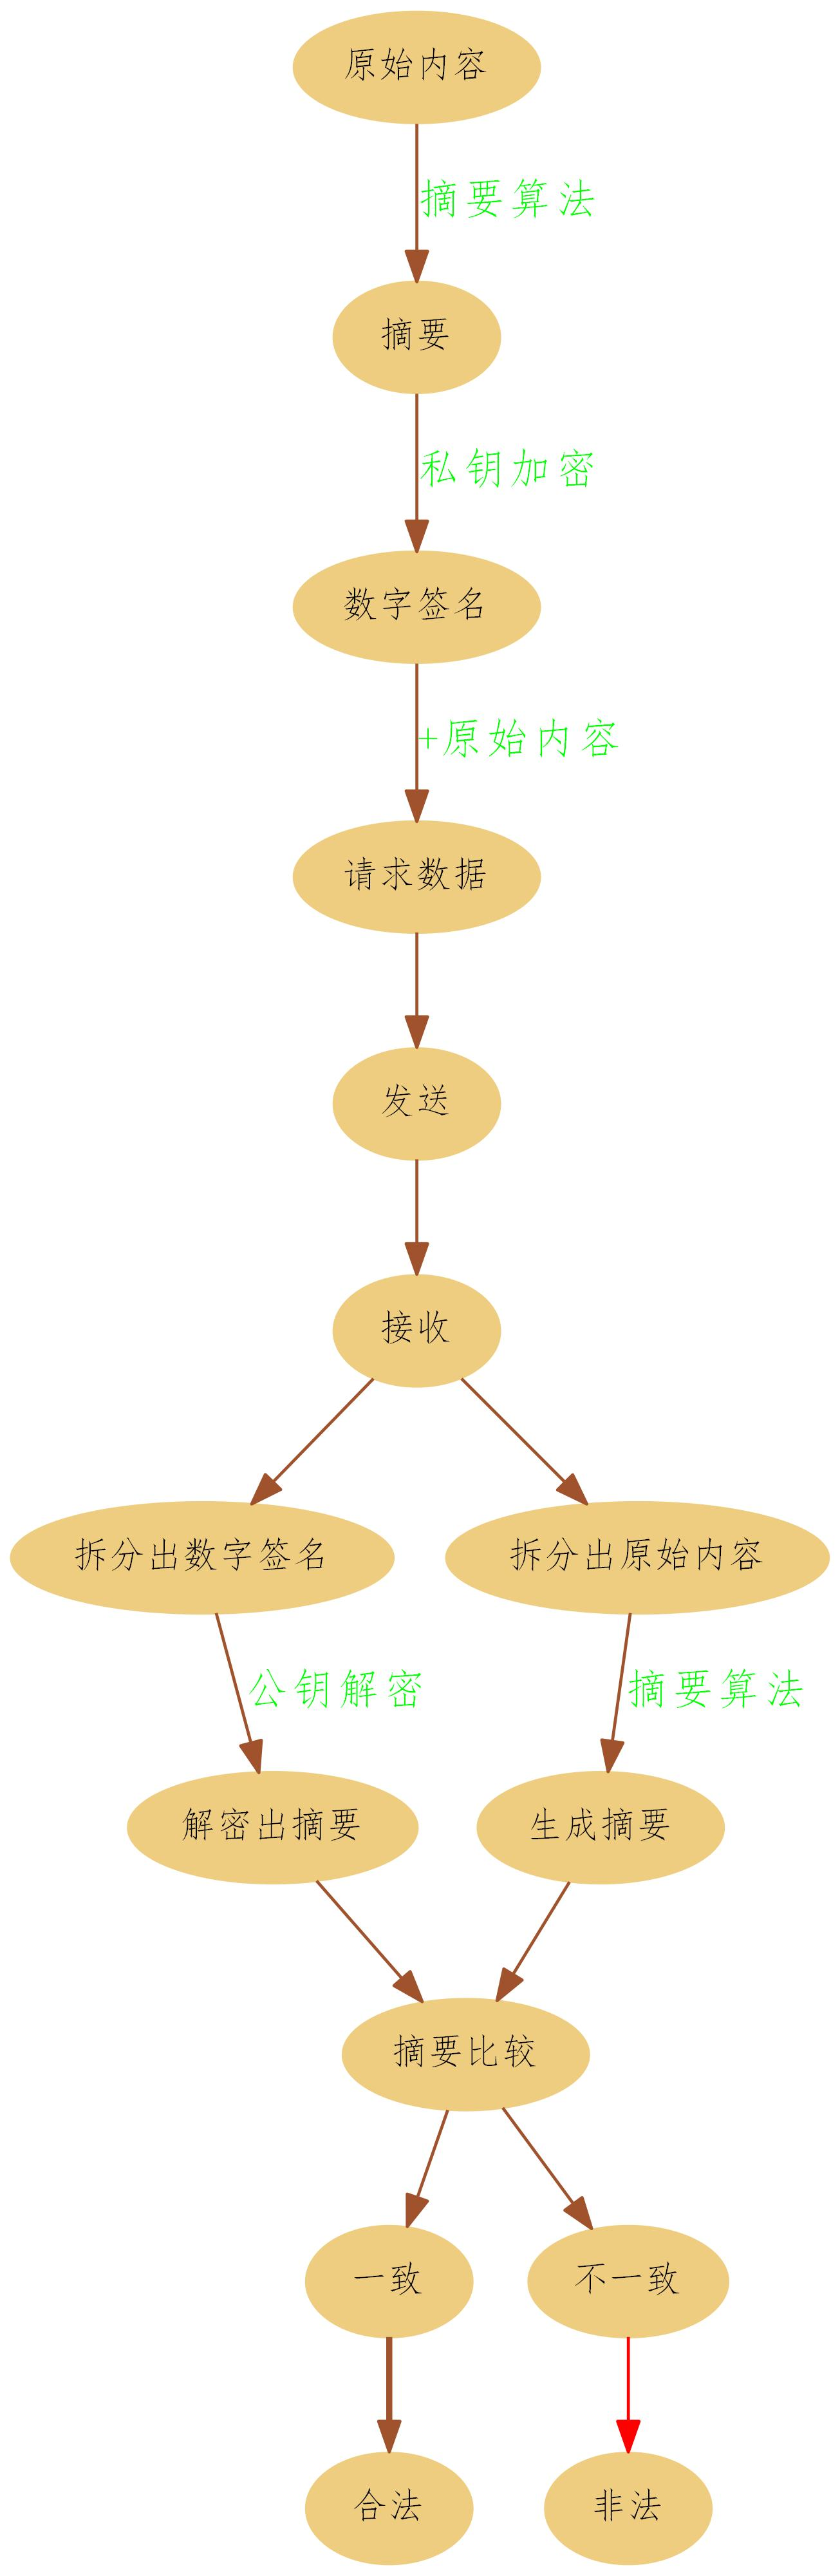
\includegraphics[scale=0.2]{ElectronicSignWorkflow.jpg}
	\caption{电子签名流程}
	\label{fig:ElectronicSignWorkflow}
\end{figure}

\subsection{SHA1算法}

安全哈希算法(Secure Hash Algorithm)主要适用于数字签名标准 (Digital Signature Standard,DSS)
里面定义的数字签名算法(Digital Signature Algorithm,DSA)。
对于长度小于2\^64位的消息,SHA1会产生一个160位的消息摘要。
当接收到消息的时候,这个消息摘要可以用来验证数据的完整性。
在传输的过程中,数据很可能会发生变化,那么这时候就会产生不同的消息摘要。 
SHA1有如下特性:不可以从消息摘要中复原信息;
两个不同的消息不会产生同样的消息摘要。
加密性强的散列一定是不可逆的,
这就意味着通过散列结果,无法推出任何部分的原始信息。

\subsection{生成签名}

代码片段\ref{code:SHA1GenerateSign}展示使用SHA1算法生成数字签名,
注意生成数字签名尽量不选择SHA1算法,
此算法被证明是不够安全的。

\begin{lstlisting}[language={[Sharp]C},caption=采用SHA1算法生成数字签名,label={code:SHA1GenerateSign}]
/// <summary>
/// 生成数字签名
/// </summary>
/// <param name="plaintext">原文</param>
/// <param name="privateKey">私钥</param>
/// <returns>签名</returns>
public static string HashAndSignString(string plaintext, string privateKey)
{
    UnicodeEncoding ByteConverter = new UnicodeEncoding();
    byte[] dataToEncrypt = ByteConverter.GetBytes(plaintext);
    using (RSACryptoServiceProvider RSAalg = new RSACryptoServiceProvider())
    {
        RSAalg.FromXmlString(privateKey);
        //使用SHA1进行摘要算法,生成签名
        byte[] encryptedData = RSAalg.SignData(dataToEncrypt, new SHA1CryptoServiceProvider());
        return Convert.ToBase64String(encryptedData);
    }
}
\end{lstlisting}

用ToBase64String方法可以在不丢失数据的情况下将字节数组转成字符串.
在ToBase64String方法中,会对字节数组中的连续三字节进行一次编码,
编码得的字符串长度为4位,
而且得出来的4位的字符串里面的字符肯定
是由大小写字母、数字(0~9)、+、/组成,
例如有一个字节数组 {212,36,25,23,45,65},
ToBase64String方法会将这个数组分成2个数组,
分别为{212,36,25}和 {23,45,65},
{212,36,25}计算出来的字符串是“1CQZ”,而{23,45,65} 是“Fy1B”,
如果是{212,36,25,23},则先分成两个数组,
{212,36,25}和{23},{212,36,25}已经计算过了,
但{23}不足三字节,怎么办?{23}会转换成“Fw==”,
所以{212,36,25}和{23,45,65},
{212,36,25}转换出来的字符串是“1CQZFy1B”,
{212,36,25,23}是“1CQZFw==”。

\subsection{验证签名}


\section{Cookie窃取(Cookie Hijacking)}

\subsection{XSS漏洞}

XSS又称CSS,全称Cross SiteScript,跨站脚本攻击,
是Web程序中常见的漏洞,XSS属于被动式且用于客户端的攻击方式,
所以容易被忽略其危害性。其原理是攻击者向有XSS漏洞的网站中输入(传入)恶意的HTML代码,
当其它用户浏览该网站时,这段HTML代码会自动执行,
从而达到攻击的目的。如,盗取用户Cookie、破坏页面结构、重定向到其它网站等。

如何预防呢?原则: 不相信客户输入的数据
注意:  攻击代码不一定在<script></script>中

\begin{itemize}
\item{将重要的cookie标记为http only,这样的话Javascript中的document.cookie语句就不能获取到cookie了}
\item{只允许用户输入我们期望的数据。 例如: 年龄的textbox中,只允许用户输入数字}
\item{而数字之外的字符都过滤掉。对数据进行Html Encode处理过滤或移除特殊的Html标签,
例如: <script>, <iframe> , \&lt; for <, \&gt; for >, 
\&quot for过滤JavaScript 事件的标签。例如 "onclick=", "onfocus" 等等}
\end{itemize}

\subsection{跨站请求伪造—CSRF}

<img src="http://bank.example.com/withdraw?account=bob\&amount=1000000\&for=mallory">

CSRF主要是黑客将伪造的请求URL放到一个图片或者其他静态资源里,这种成本极低,且传播性和形象力非常大。
举例:Qzone的签名的修改地址是:http://qzone.qq.com/cgi-bin/modify?nick=123

\subsection{Google Chrome Cookie读取}

Chrome浏览器版本33以上对Cookies进行了加密,
用SQLite Developer打开Chrome的Cookies文件就会发现,
原来的value字段已经为空,取而代之的是加密的encrypted\_value。
Chrome浏览器已保存的密码都保存在一个sqlite3数据库文件中,
和Cookies数据库在同一个文件夹。C\#中使用UnprotectData函数解密数据库中的密码字段,
即可还原密码。

\begin{lstlisting}[language={[Sharp]C},caption=解密Cookie]
byte[] sAditionalEntropy = { };
var passwordValueArray = (byte[])reader[i];
//var decryptArray = DataProtection.UnprotectData(passwordValueArray);
var decryptArray = ProtectedData.Unprotect(passwordValueArray, sAditionalEntropy, DataProtectionScope.LocalMachine);
var decryptResult = Encoding.Default.GetString(decryptArray);
row[i] = decryptResult;
\end{lstlisting}

基于ProtectedData实现的加密解密字符串,可以跨Windows用户使用,但是不能跨计算机使用。
所以在一台计算机上面加密的信息,不能在另一台计算机上面解密。
ProtectedData在System.Security.dll的命名空间System.Security.Cryptography下,
This method can be used to encrypt data such as passwords, 
keys, or connection strings. 
The optionalEntropy parameter enables you to add data to 
increase the complexity of the encryption; 
specify null for no additional complexity.
另外如果网站选择了“记住密码”选项,
Google Chrome在再次访问此网站时,
会在右上角显示一把钥匙图标,
点击钥匙图标会进入Google Chrome的Cookie密码浏览界面。
在这里也可以查看所有登录网站的密码,
不过需要输入Windows的登录密码。
也可以访问一下的链接进入Cookie密码管理界面:

\begin{lstlisting}[language=HTML]
chrome://settings/passwords
\end{lstlisting}


\section{Session劫持(Session Hijacking)}

咖啡馆的免费WiFi,就是一个很理想的劫持环境,因为两个原因:

\begin{enumerate}
\setcounter{enumi}{0}
\item{这种WiFi通常不会加密,所以很容易监控所有流量}
\item{WiFi通常使用NAT进行外网和内网的地址转换,所有内网客户端都共享一个外网地址。这意味着,被劫持的Session,看上去很像来自原来的登录者}
\end{enumerate}

\section{HTTPS}

\subsection{TLS历史}

1994年,NetScape公司设计了SSL协议(Secure Sockets Layer)的1.0版,但是未发布。
1995年,NetScape公司发布SSL 2.0版,很快发现有严重漏洞。
1996年,SSL 3.0版问世,得到大规模应用。
1999年,互联网标准化组织ISOC接替NetScape公司,发布了SSL的升级版TLS 1.0版。
2006年和2008年,TLS进行了两次升级,分别为TLS 1.1版和TLS 1.2版。最新的变动是2011年TLS 1.2的修订版。

目前,应用最广泛的是TLS 1.0,接下来是SSL 3.0。但是,主流浏览器都已经实现了TLS 1.2的支持。
TLS 1.0通常被标示为SSL 3.1,TLS 1.1为SSL 3.2,TLS 1.2为SSL 3.3。
SSL/TLS协议的基本思路是采用公钥加密法,也就是说,客户端先向服务器端索要公钥,
然后用公钥加密信息,服务器收到密文后,用自己的私钥解密。

\section{密码哈希加盐(Salted Password Hashing)}

随机盐的优势是,即使对方知道算法,也很难搞,
因为对应于每一份盐,都得花时间空间去生成对应的密码表(或者彩虹表),
也就是说一个密码表只能破解一个用户的密码,
这还是建立在已经得到数据库和加密算法的情况下,
成本瞬间高了几个数量级。
只有加密hash函数(cryptographic hash functions)可以用来进行密码的hash。
这样的函数有SHA256, SHA512, RipeMD, WHIRLPOOL等。
如下代码片段\ref{code:GenerateRandomSaltValue}生成一个随机的盐值。

\begin{lstlisting}[language={[Sharp]C},caption=生成随机盐,label={code:GenerateRandomSaltValue}]
/// <summary>
/// Creates a salted PBKDF2 hash of the password.
/// </summary>
/// <param name="password">The password to hash.</param>
/// <returns>The hash of the password.</returns>
public static string CreateHash(string password)
{
    // Generate a random salt
    RNGCryptoServiceProvider csprng = new RNGCryptoServiceProvider();`\makeremark{RNG为Random Number Generator的缩写,生成随机数还可以用Radom类,不过还不够随机,Pseudo-random numbers are chosen with equal probability from a finite set of numbers. The chosen numbers are not completely random because a definite mathematical algorithm is used to select them, but they are sufficiently random for practical purposes. The current implementation of the Random class is based on a modified version of Donald E. Knuth's subtractive random number generator algorithm. For more information, see D. E. Knuth. " The Art of Computer Programming, volume 2: Seminumerical Algorithms". Addison-Wesley, Reading, MA, second edition, 1981.}`
    byte[] salt = new byte[SALT_BYTES];
    csprng.GetBytes(salt);`\makeremark{此处即完成了生成一个随机盐,SALT\_BYTES为随机盐的长度}`

    // Hash the password and encode the parameters
    byte[] hash = PBKDF2(password, salt, PBKDF2_ITERATIONS, HASH_BYTES);
    return "sha1:" + PBKDF2_ITERATIONS + ":" +
        Convert.ToBase64String(salt) + ":" +
        Convert.ToBase64String(hash);
}
\end{lstlisting}

\showremarks

加盐可以让攻击者无法使用查表和彩虹表(Rainbow Tables)的方式对大量hash进行破解。
但是依然无法避免对单个hash的字典和暴力攻击。
高端的显卡(GPU)和一些定制的硬件每秒可以计算数十亿的hash,
所以针对单个hash的攻击依然有效。
为了避免字典和暴力攻击,我们可以采用一种称为key扩展(key stretching)的技术。
思路就是让hash的过程便得非常缓慢,
即使使用高速GPU和特定的硬件,字典和暴力破解的速度也慢到没有实用价值。
通过减慢hash的过程来防御攻击,但是hash速度依然可以保证用户使用的时候没有明显的延迟。
代码片段\ref{code:GenerateHashCodeBySaltValue}使用PBKD2算法由随机盐生成密码的Hash。

\begin{lstlisting}[language={[Sharp]C},caption=根据随机盐和密码生成Hash,label={code:GenerateHashCodeBySaltValue}]
/// <summary>
/// Computes the PBKDF2-SHA1 hash of a password.
/// </summary>
/// <param name="password">The password to hash.</param>
/// <param name="salt">The salt.</param>
/// <param name="iterations">The PBKDF2 iteration count.</param>
/// <param name="outputBytes">The length of the hash to generate, in bytes.</param>
/// <returns>A hash of the password.</returns>
private static byte[] PBKDF2(string password, byte[] salt, int iterations, int outputBytes)
{
    Rfc2898DeriveBytes pbkdf2 = new Rfc2898DeriveBytes(password, salt);
    pbkdf2.IterationCount = iterations;`\makeremark{定义生成hash的迭代次数,这个值决定了hash的过程具体有多慢,防止高速GPU的暴力破解}`
    return pbkdf2.GetBytes(outputBytes);`\makeremark{PBKDF2为Password-Based Key Derivation Function 2的缩写,假如攻击一个密码所需的Rainbow Table有1千万条,建立所对应的Rainbow Table所需要的时间就是115天。这个代价足以让大部分的攻击者忘而生畏。美国政府机构已经将这个方法标准化,并且用于一些政府和军方的系统。}`
}
\end{lstlisting}

\showremarks

\subsection{Base64编码}

Base64是网络上最常见的用于传输8Bit字节代码的编码方式之一,
大家可以查看RFC2045~RFC2049,上面有MIME的详细规范。
Base64编码可用于在HTTP环境下传递较长的标识信息。
例如,在Java Persistence系统Hibernate中,
就采用了Base64来将一个较长的唯一标识符(一般为128-bit的UUID)编码为一个字符串,
用作HTTP表单和HTTP GET URL中的参数。在其他应用程序中,
也常常需要把二进制数据编码为适合放在URL(包括隐藏表单域)中的形式。
此时,采用Base64编码具有不可读性,即所编码的数据不会被人用肉眼所直接看到。
Base64在C\#中的编码解码如下代码片段所示。

\begin{lstlisting}[language={[Sharp]C}]
//编码
byte[] bytes = Encoding.Default.GetBytes("要转换的字符");
string str = Convert.ToBase64String(bytes);
//解码
byte[] outputByte = Convert.FromBase64String(str);
string originalStr = Encoding.Default.GetString(outputByte);
\end{lstlisting}

某些RESTful接口的授权信息采用Base64编码的方式,
将验证信息经过Base64加密后存放在Http请求头中,
在Fiddler中查看请求头中的授权信息如图\ref{fig:HttpHeaderAuthorizationInfo}所示。

\begin{figure}[htbp]
	\centering
	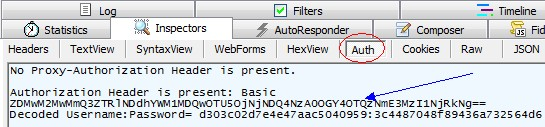
\includegraphics[scale=0.8]{HttpHeaderAuthorizationInfo.jpg}
	\caption{Http请求头中的Base64加密验证信息}
	\label{fig:HttpHeaderAuthorizationInfo}
\end{figure}

\section{SQL注入(SQL Injection)}

SQL Injection为网络安全中漏洞中,发生次数最多的漏洞。
主要是在输入SQL语法中,插入恶意的数据库查询语法。
采用完全参数化的设计,过滤使用者输入的内容。


\subsection{参数化SQL语句}

\subsubsection{正则表达校验用户输入}

\subsubsection{参数化SQL语句}

\subsubsection{替换特殊字符}

\subsection{Sqlmap}

sqlmap is an open source penetration testing tool that automates 
the process of detecting and exploiting SQL injection flaws and 
taking over of database servers. It comes with a powerful detection engine, 
many niche features for the ultimate penetration tester and 
a broad range of switches lasting from database fingerprinting, 
over data fetching from the database, to accessing the 
underlying file system and executing commands on the 
operating system via out-of-band connections.

\paragraph{基础使用}



\begin{lstlisting}[language=Bash]
./sqlmap.py -u "http://www.target.com/vuln.php?id=1" -v 1 –dbs
\end{lstlisting}

\section{Nmap(GNU General Public License)}

Nmap(Network Mapper),网络映射器,是一款开放源代码的网络探测和安全审核的工具。
它的设计目标是快速地扫描大型网络,当然用它扫描单个主机也没有问题。
Nmap以新颖的方式使用原始IP报文来发现网络上有哪些主机,
那些主机提供什么服务(应用程序名和版本),那些服务运行在什么操作系统(包括版本信息),
它们使用什么类型的报文过滤器/防火墙,以及一堆其它功能。虽然Nmap通常用于安全审核,
许多系统管理员和网络管理员也用它来做一些日常的工作,比如查看整个网络的信息,
管理服务升级计划,以及监视主机和服务的运行。
Nmap脚本引擎(Nmap Script Engine)是Nmap最有力灵活的的一个特性。
它允许用户撰写和分享一些简单的脚本来一些较大的网络进行扫描任务。
基本上这些脚本是用Lua编程语言来完成的。通常Nmap的脚本引擎可以完成很多事情。

\subsection{主机发现(Host Discovery)}

主机发现顾名思义就是发现所要扫描的主机是否是正在运行的状态。
输入如下命令开始主机扫描

\begin{lstlisting}[language=Bash]
nmap -F -sT -v nmap.org
# 主机发现,生成存活主机列表
nmap -sn -T4 -oG Discovery.gnmap 192.168.24.0/24
grep "Status: Up" Discovery.gnmap | cut -f 2 -d ' ' > LiveHosts.txt
\end{lstlisting}

\begin{itemize}
\item{-F}扫描100个最有可能开放的端口,F表示快速模式(Fast Model),
比默认模式扫描更少的端口(Scan fewer ports than the default scan),
如果需要扫描更多的端口,指定p参数,如下命令行片段所示:

\begin{lstlisting}[language=Bash]
nmap -p 0-10000 -A -v <Host>
\end{lstlisting}

端口号最好分段指定,否则扫描的速度会非常缓慢,
例如需要扫描0-65535端口,可以先扫描0-10000端口,
再扫描10001-20000,依次类推。

\item{-v}获取扫描的信息
\item{-sT(Scan using TCP)}采用的是TCP扫描,不写也是可以的,默认采用的就是TCP扫描
\item{-sn参数表示ping扫描,禁用端口扫描}
\item{-oG表示输出Grepable格式}
\end{itemize}

Nmap输出的是扫描目标的列表,以及每个目标的补充信息,至于是哪些信息则依赖于所使用的选项。
“所感兴趣的端口表格”是其中的关键。那张表列出端口号,协议,服务名称和状态。
状态可能是 open(开放的),filtered(被过滤的), closed(关闭的),或者unfiltered(未被过滤的)。
Open(开放的)意味着目标机器上的应用程序正在该端口监听连接/报文。 
filtered(被过滤的) 意味着防火墙,过滤器或者其它网络障碍阻止了该端口被访问,
Nmap无法得知 它是 open(开放的) 还是 closed(关闭的)。 
closed(关闭的) 端口没有应用程序在它上面监听,但是他们随时可能开放。 
当端口对Nmap的探测做出响应,但是Nmap无法确定它们是关闭还是开放时,
这些端口就被认为是 unfiltered(未被过滤的) 如果Nmap报告状态组合 
open|filtered 和 closed|filtered时,那说明Nmap无法确定该端口处于两个状态中的哪一个状态。
当要求进行版本探测时,端口表也可以包含软件的版本信息。
当要求进行IP协议扫描时 (-sO),Nmap提供关于所支持的IP协议而不是正在监听的端口的信息。
获取远程主机的系统类型及开放端口:

\begin{lstlisting}[language=Bash]
nmap -sS -P0 -sV -O <target>
\end{lstlisting}

\subsection{端口扫描(Port Scanning)}

端口扫描是Nmap最基本最核心的功能,用于确定目标主机的TCP/UDP端口的开放情况。
端口扫描简单示例如下代码片段所示:

\begin{lstlisting}[language=Bash]
#服务扫描
nmap-T4 -sV targetip 

#扫描淘宝IP
nmap -p 0-1000 -v 218.201.46.124
nmap -T4 -A -v 218.201.46.124
\end{lstlisting}

通过扫描可以发现一些主机信息,比如淘宝的数字证书用的是GlobalSign,
加密位数是2048,签名算法是sha256WithRSAEncryption,
操作系统猜测是Linux系列的,内核版本可能是3.X或者2.6.X,
具体信息如下。

\begin{lstlisting}
443/tcp open  ssl/http Tengine httpd
|_http-server-header: Tengine
|_http-title: 501 Not Implemented
| ssl-cert: Subject: commonName=*.tmall.com/organizationName=Alibaba (China) Technology Co., Ltd./stateOrProvinceName=ZheJiang/countryName=CN
| Issuer: commonName=GlobalSign Organization Validation CA - SHA256 - G2/organizationName=GlobalSign nv-sa/countryName=BE
| Public Key type: rsa
| Public Key bits: 2048
| Signature Algorithm: sha256WithRSAEncryption
| Not valid before: 2015-12-14T10:38:38
| Not valid after:  2016-12-14T10:38:38
| MD5:   5d67 3ca3 7f0e 2ab7 7b4f 59d5 0700 7223
|_SHA-1: d048 e9cf 5487 5030 9f26 e638 7d3f 94ad a2b3 e6fa
\end{lstlisting}

默认情况下,Nmap会扫描1000个最有可能开放的TCP端口。

1)公认端口(0~1023),又称常用端口,为已经公认定义或为将要公认定义的软件保留的。
这些端口紧密绑定一些服务且明确表示了某种服务协议。如80端口表示HTTP协议。
2)注册端口(1024~49151),又称保留端口,这些端口松散绑定一些服务。
3)动态/私有端口(49152~65535)。理论上不应为服务器分配这些端口。
按协议类型可以将端口划分为TCP和UDP端口。
1)TCP端口是指传输控制协议端口,需要在客户端和服务器之间建立连接,
提供可靠的数据传输。如Telnet服务的23端口。
2)UDP端口是指用户数据包协议端口,不需要在客户端和服务器之间建立连接。
常见的端口有DNS服务的53端口。
有的服务器为了安全会修改默认端口,
比如将ssh默认的22端口修改为50000,
不过通过Nmap扫描也会很容易的发现。
详细的扫描指令如下所示:

\begin{lstlisting}[language=Bash]
nmap -sS -sU -T4 -A -v -PE -PP -PS80,443 -PA3389 -PU40125 -PY -g 53 --script "default or (discovery and safe)" 12.26.32.14 
\end{lstlisting}

\begin{itemize}
	\item{-sS参数(TCP SYN Scan)可以利用基本的SYN扫描方式探测其端口开放状态}
	\item{-sU参数代表UDP Scan}
	\item{-T<0-5>: Set timing template (higher is faster)}
	\item{-A: Enable OS detection, version detection, script scanning, and traceroute}
	\item{-v: Increase verbosity level (use -vv or more for greater effect)}
	\item{-PE/PP/PM: ICMP echo, timestamp, and netmask request discovery probes}
	\item{-PS/PA/PU/PY[portlist]: TCP SYN/ACK, UDP or SCTP discovery to given ports}
	\item{-g/--source-port <portnum>: Use given port number}
\end{itemize}


\paragraph{"ppp0" is not an ethernet device}在使用nmap扫描时候,提示 

\begin{lstlisting}
Only ethernet devices can be used for raw scans on Windows, and "ppp0" is not an ethernet device. Use the --unprivileged option for this scan. QUITTING!
\end{lstlisting}

因为用Nmap扫描时,不能用pppoe的拨号口,只能用以太网口。
根据提示带参数--unprivileged就可以了,注意扫描的命令不能带-A参数,
否则会要求root权限,无法启动扫描。 


\subsection{版本侦测(Version Detection)}

版本侦测在后面添加sV(Service/Version)参数即可。

\begin{lstlisting}[language=Bash]
 -sV: Probe open ports to determine service/version info
\end{lstlisting}

\section{Metasploit Framework}

Metasploit是一款开源的安全漏洞检测工具,可以帮助安全和IT专业人士识别安全性问题,
验证漏洞的缓解措施,并管理专家驱动的安全性进行评估。




\section{AppScan}

IBM AppScan该产品是一个领先的 Web 应用安全测试工具,
曾以 Watchfire AppScan 的名称享誉业界。Rational AppScan 可自动化 Web 应用的安全漏洞评估工作,
能扫描和检测所有常见的 Web 应用安全漏洞,
例如 SQL 注入(SQL-injection)、跨站点脚本攻击(cross-site scripting)、
缓冲区溢出(buffer overflow)及最新的 Flash/Flex 应用及 Web 2.0 应用曝露等方面安全漏洞的扫描。


\subsection{操作系统侦测(Operating System Detection)}

\section{OpenVPN}





\subsection{OpenVPN配置(OpenVPN Configuration)}

OpenVPN的配置可以参考OpenVPN bible\footnote{\url{https://openvpn.net/index.php/open-source/documentation/howto.html}},
Step by Step可以参考CodePlayer上的分享\footnote{\url{http://www.365mini.com/page/14.htm}}.
在服务器上生成所有的配置(包括客户端),
将配置拷贝到客户端。


\paragraph{TLS key negotiation failed to occur within 60 seconds (check your network connectivity)}

One of the most common problems in setting up OpenVPN is that the two OpenVPN daemons on either side of the connection are unable to establish a TCP or UDP connection with each other.
This is almost a result of:

\begin{itemize}
\item{A perimeter firewall on the server's network is filtering out incoming OpenVPN packets (by default OpenVPN uses UDP or TCP port number 1194).}
\item{A software firewall running on the OpenVPN server machine itself is filtering incoming connections on port 1194. Be aware that many OSes will block incoming connections by default, unless configured otherwise.}
\item{A NAT gateway on the server's network does not have a port forward rule for TCP/UDP 1194 to the internal address of the OpenVPN server machine.}
\item{The OpenVPN client config does not have the correct server address in its config file. The remote directive in the client config file must point to either the server itself or the public IP address of the server network's gateway.}
\item{Another possible cause is that the windows firewall is blocking access for the openvpn.exe binary. You may need to whitelist (add it to the "Exceptions" list) it for OpenVPN to work.}
\item{注意所用的是TCP连接还是UDP连接,如果是采用UDP连接,子网上的NAT网关应该有一条端口转发规则: forward UDP port 1194 from my public IP address to 192.168.X.X}
\end{itemize}

查看OpenVPN的监听端口:

\begin{lstlisting}[language=Bash]
#netstat发现计算机上的监听或开放端口
netstat -an |find /i "listening"

netstat -an |find /i "1194"

#查看一下计算机到底通过哪些端口通信
netstat -an |find /i "established"
\end{lstlisting}

OpenVPN的配置认证文件的详细解释如下表所示。

\begin{tabular}{|l|l|l|l|l|}
	\hline
	\multirow{1}{*}{File Name}
	& \multicolumn{1}{c|}{Needed By}
	& \multicolumn{1}{c|}{Purpose}
	& \multicolumn{1}{c|}{Secret}\\
	\cline{1-4}
	ca.crt & server + all clients & Root CA certificate & NO \\
	\hline
	ca.key & key signing machine only & Root CA key & YES\\
	\hline
	dh{n}.pem & Server Only & Diffie Hellman parameters & NO\\
	\hline						
\end{tabular}

\subsection{添加新客户端(Add New Client)}

OpenVPN多个客户端不能共享一个密钥和证书(严格来说可以共享,但是推荐用单独的证书),
共享证书会导致不同客户端连接时获取的IP相同,建议在添加新的客户端时需生成新的密钥和证书。
切换到服务端的OpenVPN的easy-rsa目录下,执行如下命令添加新的证书。

\begin{lstlisting}[language=Bash]
#设置相应的局部环境变量,就是我们在vars.bat.sample文件中设置的内容
vars

#创建客户端证书
build-key client-aoxianghua
\end{lstlisting}

证书创建成功后,将证书拷贝到客户端config目录下,
在客户端配置文件中指定证书名称。

\begin{lstlisting}[language=Bash]
# SSL/TLS parms.
# See the server config file for more
# description.  It's best to use
# a separate .crt/.key file pair
# for each client.  A single ca
# file can be used for all clients.
ca ca.crt
cert client-aoxianghua.crt
key client-aoxianghua.key
\end{lstlisting}

\section{Windows自带VPN}

使用Windows自带VPN,省去了安装客户端和服务端的麻烦,
灰常方便。

\subsection{VPN类型}

\subsubsection{PPTP(Point to Point Tunneling Protocol,点对点隧道协议)}

默认端口号:1723,即PPTF协议。该协议是在PPP协议的基础上开发的一种新的增强型安全协议,
支持多协议虚拟专用网(VPN),可以通过密码身份验证协议(PAP)、可扩展身份验证协议(EAP)等方法增强安全性。
可以使远程用户通过拨入ISP、通过直接连接Internet或其他网络安全地访问企业网。
点对点隧道协议(PPTP)是一种支持多协议虚拟专用网络的网络技术,它工作在第二层。
通过该协议,远程用户能够通过Microsoft Windows NT工作站、Windows xp 、
Windows 2000和windows2003、windows7操作系统以及其它装有点对点协议的系统安全访问公司网络,
并能拨号连入本地ISP,通过Internet 安全链接到公司网络。
PPTP协议是点对点隧道协议,其将控制包与数据包分开,控制包采用TCP控制。
PPTP使用TCP协议,适合在没有防火墙限制的网络中使用。

\subsubsection{L2TP(Layer 2 Tunneling Protocol,第二层隧道协议)}

默认端口号:1701,L2TP是一种工业标准的Internet隧道协议,功能大致和PPTP协议类似,
比如同样可以对网络数据流进行加密。不过也有不同之处,比如PPTP要求网络为IP网络,
L2TP要求面向数据包的点对点连接;PPTP使用单一隧道,L2TP使用多隧道;
L2TP提供包头压缩、隧道验证,而PPTP不支持。

L2TP是一个数据链路层协议,基于UDP。其报文分为数据消息和控制消息两类。
数据消息用投递 PPP 帧,该帧作为L2TP报文的数据区。L2TP不保证数据消息的可靠投递,
若数据报文丢失,不予重传,不支持对数据消息的流量控制和拥塞控制。
控制消息用以建立、维护和终止控制连接及会话,L2TP确保其可靠投递,
并支持对控制消息的流量控制和拥塞控制。

L2TP是国际标准隧道协议,它结合了PPTP协议以及第二层转发L2F协议的优点,
能以隧道方式使PPP包通过各种网络协议,包括ATM、SONET和帧中继。
但是L2TP没有任何加密措施,更多是和IPSec协议结合使用,提供隧道验证。

L2TP使用UDP协议,一般可以穿透防火墙,适合在有防火墙限制、局域网用户,如公司、网吧、学校等场合使用。

PPTP和L2TP二个连接类型在性能上差别不大,如果使用PPTP不正常,那就更换为L2TP。

\subsubsection{OpenVPN}

默认端口号:1194,OpenVpn的技术核心是虚拟网卡,其次是SSL协议实现。
虚拟网卡是使用网络底层编程技术实现的一个驱动软件,安装后在主机上多出现一个网卡,
可以像其它网卡一样进行配置。服务程序可以在应用层打开虚拟网卡,如果应用软件(如IE)向虚拟网卡发送数据,
则服务程序可以读取到该数据,如果服务程序写合适的数据到虚拟网卡,应用软件也可以接收得到。
虚拟网卡在很多的操作系统下都有相应的实现,这也是OpenVpn能够跨平台一个很重要的理由。

OpenVPN使用OpenSSL库加密数据与控制信息:它使用了OpenSSL的加密以及验证功能,意味着,
它能够使用任何OpenSSL支持的算法。它提供了可选的数据包HMAC功能以提高连接的安全性。
此外,OpenSSL的硬件加速也能提高它的性能。

OpenVPN所有的通信都基于一个单一的IP端口,默认且推荐使用UDP协议通讯,同时TCP也被支持。

在选择协议时候,需要注意2个加密隧道之间的网络状况,如有高延迟或者丢包较多的情况下,
请选择TCP协议作为底层协议,UDP协议由于存在无连接和重传机制,导致要隧道上层的协议进行重传,效率非常低下。

OpenVPN是一个基于SSL加密的纯应用层VPN协议,是SSL VPN的一种,
支持UDP与TCP两种方式(说明:UDP和TCP是2种通讯协议,这里通常UDP的效率会比较高,速度也相对较快。
所以尽量使用UDP连接方式,实在UDP没法使用的时候,再使用TCP连接方式)。

由于其运行在纯应用层,避免了PPTP和L2TP在某些NAT设备后面不被支持的情况,
并且可以绕过一些网络的封锁(通俗点讲,基本上能上网的地方就能用OpenVPN)。

OpenVPN客户端软件可以很方便地配合路由表,实现不同线路(如国内和国外)的路由选择,实现一部分IP走VPN,
另一部分IP走原网络。


易用性:    PPTP > L2TP > OpenVPN

速度:      PPTP > OpenVPN UDP > L2TP > OpenVPN TCP

安全性:    OpenVPN > L2TP > PPTP

稳定性:    OpenVPN > L2TP > PPTP

网络适用性:OpenVPN > PPTP > L2TP

电脑上优先使用PPTP,无法使用可以尝试L2TP,对安全性要求高的优先使用OpenVPN。手持设备推荐使用L2TP。

PPTP:      最常用,设置最简单,大多数设备都支持;
L2TP:      支持PPTP的设备基本都支持此种方式,设置略复杂,需要选择L2TP/IPSec PSK方式,且设置预共享密钥PSK;
OpenVPN:最稳定,适用于各种网络环境,但需要安装第三方软件和配置文件,较复杂。

\subsubsection{SSTP:安全套接字隧道协议}

SSTP可以创建一个在HTTPS上传送的VPN隧道,从而消除与基于PPTP(点对点隧道协议)或L2TP(第2层隧道协议)VPN连接有关的诸多问题。
因为这些协议有可能受到某些位于客户端与服务器之间的Web代理、防火墙和网络地址转换(NAT)路由器的阻拦。
这种SSTP只适用于远程访问,不能支持站点与站点之间的VPN隧道。
微软公司希望,当IPSec VPN连接受到防火墙或路由器的阻拦后,
SSTP可以帮助客户减少与IPSec VPN有关的问题。此外,SSTP也不会产生保留的问题,
因为它不会改变最终用户的VPN控制权。
基于VPN隧道的SSTP可直接插入当前的微软VPN客户端和服务器软件的接口中。

\subsubsection{IKEv2(Internet Key Exchange v2)}

IKEv2(Internet Key Exchange v2)是一款新版的安全协议。
简单理解的话可以说和大家常见的PPTP/L2TP是差不多一类的东西。
不过IKEv2协议要比PPTP和L2TP更加优秀,将会是之后发展的方向之一。
二、IKEV2有什么优势?
Quote:
IKEv2连接在用户自身网络状况经常变化的情况下仍旧能够维持加密连接,
而不会出现频繁闪断、断开又重连之类的情况,能大大提高网络连接的稳定性。
IKEv2能够拥有比PPTP/L2TP更加高效的网络通讯效率。IKEv2是IKE(v1)的改良版,
使用了公钥证书和密码等多重认证,弥补了v1时代的安全性上的不足。比PPTP/L2TP更是可靠许多。
同时IKEv2还支持硬件加速,保证了高效的传输效率。
三、IKEV2的局限:
Quote:
优势和局限总是相对的,新技术面临的问题就是各方面的支持性。
现阶段提供IKEv2协议连接的VPN商家并不多,或者也可以说很少,选择余地也很小。
对于用户来说Windows 7以上包括RT系统都对IKEv2有原生支持,
Android需要第三方软件才可以支持,iOS仅支持IKEv1,
而Windows Phone干脆仅支持IKEv2协议的VPN连接。

IKE(v1)传输效率大大超于PPTP和L2TP,但仍然存在某种安全隐患。
IKEv2是IKE(v1)的全新改良版,使用公钥证书和密码等多重认证,
支持硬件加速,保持了高效的传输效率。如果出门在外,(手机)网络环境(IP 地址)经常变动的情况下,
IKEv2 是唯一使用 “MOBIKE” – Mobility and Multihoming 技术来达到加密通讯不中断目的的。
所以用户再也无需考虑手动开启或者关闭VPN,或者担心因网络环境变化而导致的VPN连接中断了。

\subsection{常见错误}

\paragraph{Error 800:未建立远程链接,因为尝试的VPN隧道失败。VPN服务器可能无法访问。如果该连接尝试使用L2TP/IPSec隧道,则IPSec协议所需的安全参数可能配置错误。}
由于Windows2000/XP/2003 系统缺省情况下启动了IPSec功能,因此在发起VPN请求时应禁止IPSec功能,
为什么要如此还无从知晓,此时需要更改注册表,
在cmd中执行regedit,找到如下路径
\begin{lstlisting}
[HKEY_LOCAL_MACHINE\SYSTEM\CurrentControlSet\Services\RasMan\Parameters]
\end{lstlisting}

新建一个键值,名称ProhibitIPSec,类型dword,值1。
或者执行如下脚本:

\begin{lstlisting}[language=Bash]
Windows Registry Editor Version 5.00
[HKEY_LOCAL_MACHINE\SYSTEM\CurrentControlSet\services\RasMan\Parameters]
"ProhibitIpSec"=dword:00000001
\end{lstlisting} 

键值修改成功后重新启动计算机即可成功连接VPN。

\paragraph{Error 809}VPN类型选择自动。

\paragraph{Error 720: Unable to establish a connection to the remote computer. Might need to change the network settings for this connection}

出现此错误原因不明,解决此错误需要在服务端配置VPN连接的IP范围,
Open Network and Sharing Center and click Change Adapter Settings.
Find Incoming Connection and right-click on it and click Properties.
具体配置如图\ref{fig:ConfigurationVPNIPAddressRange}所示。

\begin{figure}[htbp]
	\centering
	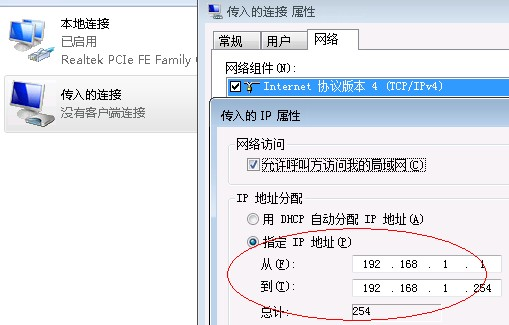
\includegraphics[scale=0.8]{ConfigurationVPNIPAddressRange.jpg}
	\caption{配置VPN客户端连接的IP范围}
	\label{fig:ConfigurationVPNIPAddressRange}
\end{figure}

如果VPN服务端在局域网中,在传入的IP属性中指定IP地址段时从192.168.1.2开始(图中的IP需要修改),
因为192.168.1.1为路由器的地址,从192.168.1.1开始会导致VPN服务器会分配到路由器的默认IP,
导致路由器的部分功能不可用。

\section{DIRB}

DIRB is a Web Content Scanner. It looks for existing (and/or hidden) Web 
Objects. It basically works by launching a dictionary based attack against 
a web server and analizing the response.

DIRB comes with a set of preconfigured attack wordlists for easy usage but 
you can use your custom wordlists. Also DIRB sometimes can be used as a 
classic CGI scanner, but remember is a content scanner not a vulnerability 
scanner.

DIRB main purpose is to help in professional web application auditing. 
Specially in security related testing. It covers some holes not covered by 
classic web vulnerability scanners. DIRB looks for specific web objects that 
other generic CGI scanners can't look for. It doesn't search vulnerabilities 
nor does it look for web contents that can be vulnerables.

\section{Network}

\subsection{Ubuntu 使用aircrack破解WiFi}

破解原理:直接把这段握手包给截取下来,在本地验证好了再发给热点就行。
无线路由器的另一种加密方式为WPA/WPA2加密,相比较于WEP加密,
暂时未能从一些公开的方法中找到直接破解WPA/WPA2密码的方法,
只能先抓获握手包,然后对握手包进行暴力破解,但是结合着一些技巧以及普通用户密码策略比较薄弱,成功的机率也比较高。
抓握手包跑字典,这主要看你的字典给不给力了,拼人品的时间到了,
和破解wep操作一样的,选中信号点lanch开始抓包,抓包的时候路由器是一定要有用户使用,
目的是攻击导致对方掉线,在自动重连的过程中抓取WPA认证的四次握手包。
如果一直没找到在线的客户端,就抓不到包的,只能等有人用的时候再试了。
Aircrack是破解WEP/WPA/WPA2加密的主流工具之一,Aircrack-ng套件包含的工具可用于捕获数据包、握手验证。
可用来进行暴力破解和字典攻击。在Ubuntu 14.02下安装aircrack-ng:

\begin{lstlisting}[language=Bash]
apt-get install aircrack-ng
\end{lstlisting}

力破解和字典攻击。
– Aircrack-ng 无线密码破解
– Aireplay-ng 流量生成和客户端认证
– Airodump-ng 数据包捕获
– Airbase-ng  虚假接入点配置

\paragraph{启动无线网卡的监控模式}
启动无线网卡的监控模式如下:

\begin{lstlisting}[language=Bash]
sudo airmon-ng start wlan0

sudo airodump-ng -a --encrypt WPA mon0
\end{lstlisting}

无线网卡开始抓包并分析附近有那些热点(-a),
并且仅显示加密方式为WPA或者WPA2的热点(-- encrypt WPA) – 上图只需要看懂这些参数:
BSSID指一个热点(PC or Phone),你可以理解为它的ID,PWR指信号强度,越接近0越好,
但是不能等于0,0表示断线,后面将会用到,CH频道,这个也会用到,ENC加密方式,
仅显示了PSK/PSK2方式,ESSIS这个就是我们平常看到的热点名称辣

\paragraph{查看无线AP}在终端中输入:

\begin{lstlisting}[language=Bash]
sudo airodump-ng mon0
\end{lstlisting}

(mon0 是启动监控模式后无线网的端口)
查看有哪些采用wep加密的AP在线,然后按 ctrl+c 中止,不要关闭终端。

\paragraph{抓包}
打开另一个终端,输入:

\begin{lstlisting}[language=Bash]
sudo airodump-ng --channel 6 --bssid AP’s MAC -w wep mon0

sudo airodump-ng --bssid 28:2C:B2:E4:F5:5A -c 13 -w 619 --ignore-negative-one mon0
\end{lstlisting}

(-c后面跟着的6是要破解的AP工作频道,–bissid后面跟着的AP’sMAC是要欲破解AP的MAC地址,
-w后面跟着wep的是抓下来的数据包DATA保存的文件名,具体情况根据步骤2里面的在线AP更改频道和MAC地址,
DATA保存的文件名可随便命名)

本机Mac:00:25:d3:9a:b6:01

路由Mac:C0:61:18:9A:76:D2

\paragraph{与AP建立虚拟连接}
再打开一个新终端,输入:

\begin{lstlisting}[language=Bash]
aireplay-ng -2 -F -p 0841 -c ff:ff:ff:ff:ff:ff -b C0:61:18:9A:76:D2 -h 00:25:d3:9a:b6:01 mon0
\end{lstlisting}


(-h后面跟着的My MAC是自己的无线网卡的MAC地址,即ifconfig命令下wlan0对应的mac地址)

\paragraph{解密}
收集有15000个以上的DATA之后,另开一个终端,切换到aircrack-ng-1.1目录,执行以下命令
sudo aircrack-ng wep*.cap
进行解密
(如果没算出来的话,继续等,aircrack-ng 会在DATA每增加多15000个之后就自动再运行,
直到算出密码为至,注意此处文件的名字要与步骤3里面设置的名字一样,且*号是必需的)

\section{ZAP}

The OWASP Zed Attack Proxy (ZAP) is one of the world’s most popular free security tools 
and is actively maintained by hundreds of international volunteers*. 
It can help you automatically find security vulnerabilities in your web 
applications while you are developing and testing your applications. 
Its also a great tool for experienced pentesters to use for manual security testing.
使用Java语言开发。

\section{Patator}

\subsection{简介}

Patator was written out of frustration from using Hydra, 
Medusa, Ncrack, Metasploit modules and Nmap NSE scripts for password guessing attacks. 

\subsection{使用}

查看某一个协议的用法:

\begin{lstlisting}[language=Bash]
./patator.py mysql_login --help
\end{lstlisting}

其中MySQL是协议的名称。
破解MySQL登录:

\begin{lstlisting}[language=Bash]
./patator.py mysql_login host=ip user=root password=FILE0 0=dic.txt
\end{lstlisting}


\section{Hacking}

\subsection{Google Hacking}

Google hacking, also named Google dorking, 
is a computer hacking technique that uses Google Search and other 
Google applications to find security holes in the configuration and computer code that websites use.
这是一个Google搜索技巧的清单:

\begin{lstlisting}
link:URL = 列出到链接到目标URL的网页清单.
related:URL = 列出于目标URL地址有关的网页.
site:Domain Name Registration and Web Hosting 搜索区域仅限于目标网站.
allinurl:WORDS = 只显示在URL地址里有搜索结果的页面.
inurl:WORD = 跟allinurl类似,但是只在URL中搜索第一个词.
allintitle:WORD = 搜索网页标题.
intitle:WORD = 跟allintitle类似,但是只在标题里搜索第一个词.
cache:URL = 将显示关于URL的Google缓存(中国不可用).
info:URL = 将显示一个包含了这些元素的页面:类似结果的链接,反向链接,还有包括了这个URL的页面.在搜索框里直接输入URL会起到同样的效果.
filetype:SOMEFILETYPE = 指定文件类型.
-filetype:SOMEFILETYPE = 剔除指定文件类型.
site:Welcome to SomeSite.Net ! “+Welcome to SomeSite.Net !” = 显示该站点有多少网页被google收录
allintext: = 搜索文本,但不包括网页标题和链接
allinlinks: = 搜索链接, 不包括文本和标题
WordA OR WordB = 搜索包含两关键词之一的页面
“Word” OR “Phrase” = 精确的要求搜索单词或者句子
WordA -WordB = 包含单词A但是不包含单词B
WordA +WordB = 都包含
~WORD = 寻找此单词和它的同义词
~WORD-WORD = 只搜索同义词,不要原词
\end{lstlisting}

\paragraph{准确搜索(Exact phrase)}
最简单、有效的准确搜索方式是在关键词上加上双引号,在这种情况下,搜索引擎只会反馈和关键词完全吻合的搜索结果。
比方说在搜索「Joe Bloggs」的时候,在没有给关键词加上双引号的情况,
搜索引擎会显示所有分别和「Joe」以及「Bloggs」相关的信息,但这些显然并不是我们想要的结果。
但在加上双引号后,搜索引擎则仅会在页面上反馈和「Joe Bloggs」相吻合的信息。
准确搜索在排除常见但相近度偏低的信息时非常有用,可以为用户省去再度对结果进行筛选的麻烦。
使用引号来搜索一个完全匹配的字词或一组字词。在搜索歌词或文学作品中的一段文字时,此选项很实用。

\paragraph{排除关键词(Exclude terms)}
如果在进行准确搜索时没有找到自己想要的结果,用户可以对包含特定词汇的信息进行排除,仅需使用减号即可。
例如在搜索「『Joe Bloggs』-jeans」时,你所得到的结果反馈是不包含「jeans」字眼的「Joe Bloggs」条目。
在某个字词前添加短横 (-) 可排除所有包含该字词的搜索结果。在搜索像汽车品牌美洲虎和动物美洲虎这类同义词时,此功能特别实用。

\paragraph{用「Either OR」(或)逻辑进行搜索}
在默认搜索下,搜索引擎会反馈所有和查询词汇相关的结果,但通过使用「OR」逻辑,你可以得到和两个关键词分别相关的结果,而不仅仅是和两个关键词都同时相关的结果。巧妙使用「OR」搜索可以让你在未能确定哪个关键词对于搜索结果起决定作用时依然可以确保搜索结果的准确性。[OR]也可以替换成竖线(|)。

\paragraph{@}关键字前加@符号,查找社交网站上相关结果。

\paragraph{站内搜索}站内搜索语法如下:

\begin{lstlisting}
php site:http://stackoverflow.com/
\end{lstlisting}

site操作符非常有用,可以让google搜索来自指定的网站的网页。
比如,想在sourceforge.net网站上搜索关于编辑器notepad++的网页,
可以输入:"notepad++"  site:sourceforge.net。
这样google就能返回来自sourceforge.net的网页。
又比如,想查找csdn网站上关于端口扫描器Nmap的网页,
那么可以输入:"nmap"  site:csdn.net。  site操作符,可用于搜索指定网站的上特殊的信息,
如包含的主要资源,是否暴露出敏感文件等。

\paragraph{文件类型filetype}当用户单独搜索某一类文件时,
可使用该关键字。比如想搜索关于黑客技巧Hacking的PPT,
可以搜索:

\begin{lstlisting}
hacking filetype:ppt
\end{lstlisting}

如果想要搜索关于黑客大曝光系列图书的PDF,
可以尝试输入:"hacking exposed" filetype:pdf,
这样就能直接搜索很多该系列图书的PDF文档。同理,也可以结合site操作符,搜索指定网站内的资源,
如word文件、XML文件、excel文件、PPT文档、txt等等。

\paragraph{..时间范围}
两点操作符用于指定一个网页的时间范围,
比如用户想搜索的是2011年到2012年内,出现的关于web hacking的PDF资料。

可以输入:web hacking filetype:pdf 2011..2012

\paragraph{intitle:index-of}
如果只是寻找文件而不是网页,
只需用index of代替intitle:参数。
它可以帮助你寻找网络和FTP目录。
搜索某类资源的索引目录,如想搜索网站的图像、父目录等信息。
可以在google搜索:intitle:index-of image和intitle:index-of “parent directory”。
也可以搜索与Admin密切相关的网页:intitle:index-of “admin”。 
也可以尝试:intitle:index-of mp3/intitle:index-of password等查询,具体查询内容就需要靠自己想象力了。

\paragraph{限定网页标题}
网页标题往往包含了文章主旨,因此可以用intitle对搜索结果进行筛选,
只显示那些网页标题包含了特定关键字的内容。例如搜索关于莱昂纳多的内容,
但是网页标题明确包含泰坦尼克号关键字的:莱昂纳多 intitle:泰坦尼克号。

\paragraph{善用星号}

在搜索引擎中,我们可以用星号填补关键词中的缺失部分,
不论缺失的是一连串单词的其中一个还是一个单词的某一部分。
此外,当你希望搜索一篇确定性偏低的文章时,也可以使用星号填补缺失部分。

比如用关键字 Array.prototype.* 进行搜索,
前几条依次是 Array.prototype.slice(),Array.prototype.find(),
Array.prototype.sort() 相关。
再比如,对于某个人名你不确定,可以这样搜,武*兰,武初兰是什么鬼?

\paragraph{搜索相关网站}

实例:related:www.tudou.com,related:www.cnblogs.com.
这个功能比较好玩,可以搜索类似的网站,竞品网站。
比如我要搜索和土豆网类似的网站,可以这样 related:www.tudou.com,
优酷,爱奇艺,腾讯视频什么的都出来了。搜一下和博客园类似的网站?

\subsection{Shodan Hacking}

\chapter{Node.js}

\clearpage
\mbox{}         
\clearpage

\subsection{Introduce}

Node.js越来越流行,这个基于Google V8引擎建立的平台, 
用于方便地搭建响应速度快、易于扩展的网络应用。
Nodejs标准的web开发框架Express,可以帮助我们迅速建立web站点,
比起PHP的开发效率更高,而且学习曲线更低。非常适合小型网站,个性化网站。

\begin{quotation}
Node.js® is a JavaScript runtime built on Chrome's V8 JavaScript engine. 
Node.js uses an event-driven, non-blocking I/O model that makes it lightweight and efficient. 
Node.js' package ecosystem, npm, is the largest ecosystem of open source libraries in the world.
\end{quotation}

\subsection{Install}

\paragraph{Step 1}~下载nodejs,官网:\url{http://nodejs.org/download/},
我这里下载的是node-v4.1.1-x64.msi。
安装基本是下一步下一步即可完成。
当Node.js安装完成以后,npm(Node.js Package Management)也一并安装完毕。


\subsection{基础的HTTP服务器}

安装完成后项目的根目录下编写一个简单的服务器端脚本server.js\footnote{http://www.nodebeginner.org/index-zh-cn.html}。

\begin{lstlisting}[language=VBScript]
var http = require("http");

http.createServer(function(request, response) {
  response.writeHead(200, {"Content-Type": "text/plain"});
  response.write("Hello World");
  response.end();
}).listen(8888);
\end{lstlisting}

用Node运行这段代码,
然后在浏览器端访问链接\url{http://localhost:8888/}即可看到输出的Hello World。

\begin{figure}[htbp]
	\centering
	\includegraphics[scale=1]{NodeJSFirstHelloWorld.jpg}
	\caption{NodeJS Hello World}
	\label{fig:NodeJSFirstHelloWorld}
\end{figure}

第一行请求(require)Node.js自带的 http 模块,
并且把它赋值给 http 变量。
接下来我们调用http模块提供的函数: createServer 。
这个函数会返回一个对象,这个对象有一个叫做 listen 的方法,
这个方法有一个数值参数,指定这个HTTP服务器监听的端口号。

\subsection{独立出服务端的模块}

在server.js文件中有一个非常基础的HTTP服务器代码,
而且通常我们会有一个叫 index.js 
的文件去调用应用的其他模块(比如 server.js 中的HTTP服务器模块)来引导和启动应用。
把server.js变成一个真正的Node.js模块,
使它可以被 index.js 主文件使用。
将服务脚本改成如下的形式。

\begin{lstlisting}[language=VBScript]
var http = require("http");

function start() {
  function onRequest(request, response) {
    console.log("Request received.");
    response.writeHead(200, {"Content-Type": "text/plain"});
    response.write("Hello World");
    response.end();
  }

  http.createServer(onRequest).listen(8888);
  console.log("Server has started.");
}

exports.start = start;
\end{lstlisting}

现在就可以创建我们的主文件index.js并在其中启动我们的HTTP了,
虽然服务器的代码还在server.js中。
创建index.js文件并写入以下内容:

\begin{lstlisting}[language=VBScript]
var server = require("./server");
server.start();
\end{lstlisting}

\paragraph{Step 2}~安装相关环境

\begin{lstlisting}[language=Bash]
npm install -g express  
npm install -g jade
npm install -g mysql
\end{lstlisting}

安装时带上参数g,表示全局模式,
node的安装分为全局模式和本地模式。
一般情况下会以本地模式运行,
包会被安装到和你的应用程序代码的本地node\_modules目录下。
在全局模式下,Node包会被安装到Node的安装目录下的node\_modules下。
Express是NodeJS的Web开发框架。
Jade是一个高性能的模板引擎,它深受Haml影响,
它是用JavaScript实现的,并且可以供Node使用。
CoffeeScript是一套JavaScript的转译语言,
创建者Jeremy Ashkenas戏称它是JavaScript的不那么铺张的小兄弟。
因为CoffeeScript会将类似 Ruby 语法的代码编译成 JavaScript,
而且大部分结构都相似,但不同的是 CoffeeScript 拥有更严格的语法。
如图所示表示安装完毕。

\begin{figure}[htbp]
	\centering
	\includegraphics[scale=1]{NodeJSInstallCompelete.jpg}
	\caption{Node JS Install Complete}
	\label{fig:NodeJSInstallCompelete}
\end{figure}


\subsection{服务端路由}

将server.js脚本改成如下的形式。

\begin{lstlisting}[language=VBScript]
var http = require("http");
var url=require("url");
function start(route){
	function onRequest(request,response){
		var pathname=url.parse(request.url).pathname;		
		console.log("Request for " + pathname + " received.");		
		route(pathname);		
		console.log("Request recieved.");
		response.writeHead(200, {"Content-Type": "text/plain"});
		response.write("Hello World");
		response.end();
	}	
	http.createServer(onRequest).listen(8888);
	console.log("Server has started.");
}
exports.start=start;
\end{lstlisting}

\subsection{NodeJS RESTful Service}

NodeJS提供RESTful接口,此段代码直接定义一个集合资源进行返回。

\begin{lstlisting}[language=VBScript]
var express = require("express") //加载模块
var app = express() //实例化之
var map = {"list1":{id:1,name:"Pen"},"list2":{id:2,name:"Pencil"}} //定义一个集合资源
app.get("/devices",function(request, response){ //Restful Get方法,查找整个集合资源
    response.set({"Content-Type":"text/json","Encodeing":"utf8"});
    response.send(map)
})

app.get("/devices/:id",function(request, response){ //Restful Get方法,查找一个单一资源
    response.set({"Content-Type":"text/json","Encodeing":"utf8"});
    response.send(map[request.param("id")])
    //console.log(request.param("id"))
})
app.listen(8888); //监听8888端口
\end{lstlisting}

将此段代码写入restfulServer.js文件中,
用node命令加载此段代码,
用浏览器请求链接http://localhost:8888/devices即可获取定义的资源。
如果需要获取特定的集合,
添加ID即可,链接为http://localhost:8888/devices/{ID}。

\subsection{NodeJS connect SQL Server}

NodeJS连接SQL Server需要下载依赖包node-sqlserver,
node-sqlserver是微软官方发布的SQL Server的Node.js的驱动程序。
可允许Windows上运行的Node.js程序访问SQL Server和Windows Azure SQL数据库。

\begin{lstlisting}[language=Bash]
#查看当前项目的本地依赖包
npm list

#查看全局依赖包
npm list -g 

#安装node-gyp
npm install -g node-gyp

#查找与sqlserver有关的包
npm find sqlserver

#下载node-sqlserver包
npm install node-sqlserver -g
\end{lstlisting}

注意安装node-sqlserver时gyp工具依赖与Python,
所以还需要安装Python,
且Python的版本要求为:>=2.5.0\&<3.0.0。

\begin{lstlisting}[language=VBScript]
var sql = require("node-sqlserver");

var connectionString = "Driver={SQL Server Native Client 11.0};Server={.};Database={rr-ccn};Trusted_Connection={Yes};uid=sa;PWD=123456;";

sql.open(connectionString, function(err, conn) {
    if(err) {
        // error handler code
    }
    else {
        // do what you want to do to this database
        sql.queryRaw(connectionString, "select * from users", function (err, results) {
            if (err) {
                console.log(err);
            }
            else {
                for (var i = 0; i < results.rows.length; i++) {
                    console.log(results.rows[i][0] + results.rows[i][1]);
                }
            }
        })
    }
});
\end{lstlisting}

http://geekswithblogs.net/shaunxu/archive/2012/09/17/node.js-adventure---node.js-with-sql-server.aspx

安装mssql包。

\begin{lstlisting}[language=Bash,caption=npm操作脚本]
#安装mssql包
npm install mssql -g

#安装mssql包到本地,安装mssql包到全局时会提示找不到mssql模块
npm install mssql --local

#或者将全局的包和本地的项目链接起来,mssql为包名
npm link mssql

#强制指定链接为本地链接
npm link mssql --local
\end{lstlisting}

一个连接数据库的例子,
index.js文件的内容如下。

\begin{lstlisting}[language=VBScript]
var server=require("./server");
server.start();
\end{lstlisting}

server.js的内容如下,此段代码展示最简单的使用mssql连接sql server数据库。

\begin{lstlisting}[language=VBScript]
var http = require("http");
var sql = require("mssql");

var config = {
    user: "renren",
    password: "renren!@#321",
    server: "129.29.81.129", // You can use "localhost\\instance" to connect to named instance
    port:"5001",
    database: "renren-weixin",
    options: {
        encrypt: false /* Use this if you"re on Windows Azure*/
    }
}

function start(){
    var connection = new sql.Connection(config, function(err) {
        var request = new sql.Request(connection); \\ or: var request = connection.request();
        request.query("select top 1 * from tb_printMac", function(err, recordset) {           
            console.log(err);
            console.dir(recordset);
        });
    });
    console.log("Server has started.");
}
exports.start=start;
\end{lstlisting}

\subsection{配置文件管理}

NodeJS配置文件可以通过JavaScript和Json格式的文件进行管理,
通过Json格式管理,新建package.json文件,
内容如代码\ref{code:NodeJSJsonConfig}所示。

\begin{lstlisting}[language={[Sharp]C},caption=NodeJS json格式配置,label={code:NodeJSJsonConfig}]
{
    "name": "rrmallrestapi",
    "version": "0.0.1",
    "dbconnstring":
    {
        "renrenweixin":
        {
            "user": "renren-admin",
            "password": "renren-admin!@#321",
            "server": "129.20.84.118",
            "port":"5002",
            "database": "renren-weixin"
        }        
    }
}
\end{lstlisting}

在JavaScript中读取方式如下所示,

\begin{lstlisting}[language=VBScript]
var sysconfig=require("./../../config/package.json");

var config = {
    user: sysconfig.dbconnstring.renrenweixin.user,
    password: sysconfig.dbconnstring.renrenweixin.password,
    server: sysconfig.dbconnstring.renrenweixin.server, 
    port:sysconfig.dbconnstring.renrenweixin.port,
    database: sysconfig.dbconnstring.renrenweixin.database,
    options: {
        encrypt: false
    }
}
\end{lstlisting}

\subsection{Debug}

安装supervisor。

\begin{lstlisting}[language=Bash]
#查找可用包
npm find packageName

npm install supervisor -g
\end{lstlisting}

\subsection{exports}

如果你想你的模块是一个特定的类型就用Module.exports。
如果你想的模块是一个典型的“实例化对象”就用exports。

\subsection{处理POST请求}

\subsection{Express}

Express\footnote{http://expressjs.com/}是一个基于 Node.js 平台的极简、灵活的 web 应用开发框架,
它提供一系列强大的特性,帮助你创建各种 Web 和移动设备应用。 

\begin{lstlisting}[language=Bash]
#安装express
npm install express -g

#安装express-generator,从express 4.x版本中将命令工具分出来了,需要再安装一个命令工具
#否则expresss命令无法使用
npm install express-generator -g 
\end{lstlisting}

进入工程目录,使用express命令创建工程\footnote{http://blog.fens.me/nodejs-express3/}。

\begin{lstlisting}[language=Bash]

D:\workspace\project>express -e nodejs-demo

cd nodejs-demo && npm install


D:\workspace\project\nodejs-demo>node app.js

D:\workspace\project\nodejs-demo>supervisor app.js

\end{lstlisting}


\begin{figure}[htbp]
	\centering
	\includegraphics[scale=1]{StartTemplateProject.jpg}
	\caption{Node JS Install Complete}
	\label{fig:StartTemplateProject}
\end{figure}

\begin{figure}[htbp]
	\centering
	\includegraphics[scale=1]{StartPortSuccess.jpg}
	\caption{NodeJS Express Install Complete}
	\label{fig:StartPortSuccess}
\end{figure}


node\_modules, 存放所有的项目依赖库。(每个项目管理自己的依赖,与Maven,Gradle等不同)
package.json,项目依赖配置及开发者信息
app.js,程序启动文件
public,静态文件(css,js,img)
routes,路由文件(MVC中的C,controller)
Views,页面文件(Ejs模板)

\subsection{MEAN}

\subsubsection{MongoDB}

安装完毕后进入MongoDB的安装目录,
运行如下命令初始化MongoDB。

\begin{lstlisting}[language=Bash]
cd C:\Program Files\MongoDB\Server\3.0\bin
mongod -dbpath "d:\DB"
\end{lstlisting}

dbpath参数指定MongoDB的路径为d:\textbackslash DB,
运行如下命令启动MongoDB。

\begin{lstlisting}[language=Bash]
cd C:\Program Files\MongoDB\Server\3.0\bin
mongo
\end{lstlisting}


show dbs    显示数据库列表

use dbname    进入dbname数据库,大小写敏感,没有这个数据库也不要紧

show collections    显示数据库中的集合,相当于表格


\section{常用脚本}

\subsection{BAT}

\begin{lstlisting}[language=Bash]
#递归列出当前目录下所有的备份文件,保存到txt文件中
dir *.bak /s>a.txt
\end{lstlisting}

\chapter{异常(Exception)}

\clearpage
\mbox{}         
\clearpage

在早期的Win32 API设计中是通过返回true/false来表示一个过程(方法、函数)是否执行成功,
在COM中是使用HRESULT来表示一个过程是否正确执行,
然而这种处理异常的方式使开发人员对哪里出错,为什么出错,出什么样的错这些问题很难找到明确的答案,
再一点,调用者很容易忽略一个过程执行的结果,如果调用者丢弃了过程执行结果,
则代码将“按照期望的状态正常执行”,这是很危险的。后来,在.NET Framework中,
已经不再使用这种简单的以状态码来表示执行结果的处理方式,而是使用抛出异常的方式来告诉调用者。
CLR中的异常是基于SEH(Structured Exception Handling)的结构化异常处理机制构建的,
在基础的SEH机制中是向系统注册出错时的回调函数,
当在监视区内出错时,系统会取得当前线程的控制权处理回调函数,处理完毕后,系统释放控制权给当前线程,
当前线程继续执行,如果未处理异常的代码段,会导致进程中止。

\section{Winows SEH}

SEH(Structured Exception Handling)是Windows系统提供的功能,跟开发工具无关。值得一提的是,
VC将SEH进行了封装try catch finally,
c++中也可以用c的封装\_\_try\{\}\_\_except()\{\} 和\_\_try\{\}\_\_finally\{\}.
所以当你建立一个C++ try块时,编译器就生成一个SEH\_\_try块。
SEH是为C语言设计的,但是他们也能够被用于C++。
SEH异常由\_\_try\{\}\_\_except()\{\}结构来处理。
SEH是VC++编译器特有的,因此如果你想要编写可移植的代码,就不应当使用SEH。
一个C++ catch测试变成一个SEH异常过滤器,
并且catch中的代码变成SEH\_\_except块中的代码。
实际上,当你写一条C++ throw语句时,编译器就生成一个对Windows的Raise Exception函数的调用。
用于throw语句的变量传递给Raise Exception作为附加的参数。

SEH: 结构化异常处理
VEH: 向量化异常处理
TopLevelEH:顶层异常处理

\begin{enumerate}
\setcounter{enumi}{0}
\item{交给调试器(进程必须被调试)}
\item{\textbf{执行VEH(Vectored Exception Handling)}}~~向量化异常处理(VEH)是结构化异常处理的一个扩展,它在Windows XP中被引入。你可以使用AddVectoredExceptionHandler()函数添加一个向量化异常处理器,VEH的缺点是它只能用在WinXP及其以后的版本,因此需要在运行时检查AddVectoredExceptionHandler()函数是否存在。
\item{\textbf{执行SEH(Structured Exception Handling)}}~~当发生一个SEH异常时,你通常会看到一个意图向微软发送错误报告的弹出窗口。你可以使用RaiseException()函数自己产生一个SEH异常。你可以在你的代码中使用\_\_try\{\}\_\_except(Expression)\{\}结构来捕获SEH异常。程序中的main()函数被这样的结构保护,因此默认地,所有未被处理的SEH异常都会被捕获。
\item{TopLevelEH(进程被调试时不会被执行)}
\item{交给调试器(上面的异常处理都说处理不了,就再次交给调试器)}
\item{调用异常端口通知csrss.exe}
\end{enumerate}

\subsection{Don't ever swallow exceptions}

The worst thing you can do is catch (Exception) and put an empty code block on it. Never do this.

参照:http://www.codeproject.com/Articles/9538/Exception-Handling-Best-Practices-in-NET

\subsection{Log Exception.ToString(); never log only Exception.Message}

As we're talking about logging, don't forget that you should always log Exception.ToString(), 
and never Exception.Message. Exception.ToString() will give you a stack trace, 
the inner exception and the message. Often, this information is priceless and if you only log Exception.Message, 
you'll only have something like "Object reference not set to an instance of an object".

\subsection{异常列表(Exception List)}

\begin{tabular}{ll}
	\multirow{1}{*}{}			
	& \multicolumn{1}{c}{}\\
	ArgumentException & 该类用于处理参数无效的异常\\
	IOException & 该类用于处理进行文件输入输出操作时所引发的异常\\	
	DivideByZeroException & 表示整数十进制运算中试图除以零而引发的异常\\					
\end{tabular}

\subsection{Windows Form中统一异常处理}

适当的使用try捕获异常,异常信息建议由最上层的框架捕获,
将来修改起来相对容易,越少try...catch的程序越美。
WinFrom的Application对象本身就提供了ThreadException时间来捕捉为处理的异常

\begin{lstlisting}[language={[Sharp]C}]
static void Main()
{
    //设置应用程序处理异常方式:ThreadException处理
    Application.SetUnhandledExceptionMode(UnhandledExceptionMode.CatchException);
    //处理UI线程异常
    Application.ThreadException += new System.Threading.ThreadExceptionEventHandler(Application_ThreadException);
    //处理非UI线程异常
    AppDomain.CurrentDomain.UnhandledException += new UnhandledExceptionEventHandler(CurrentDomain_UnhandledException);    Application.EnableVisualStyles();
    Application.SetCompatibleTextRenderingDefault(false);
    Application.Run(new Form1());
}

static void Application_ThreadException(object sender, System.Threading.ThreadExceptionEventArgs e)
{
    var exceptionMessage = GetExceptionMsg(e.Exception, e.ToString());
    Log.Logger.Error(exceptionMessage);
}

static void CurrentDomain_UnhandledException(object sender, UnhandledExceptionEventArgs e)
{
    var exceptionMessage = GetExceptionMsg(e.ExceptionObject as Exception, e.ToString());
    Log.Logger.Error(exceptionMessage);
}

/// <summary>
/// 生成自定义异常消息
/// </summary>
/// <param name="ex">异常对象</param>
/// <param name="backStr">备用异常消息:当ex为null时有效</param>
/// <returns>异常字符串文本</returns>
static string GetExceptionMsg(Exception ex,string backStr)
{
    var exceptionContent = new StringBuilder();
    exceptionContent.AppendLine("***********异常文本**********");
    exceptionContent.AppendLine("【出现时间】:" + DateTime.Now.ToString(CultureInfo.InvariantCulture));
    if (ex != null)
    {
	    exceptionContent.AppendLine("【异常类型】:" + ex.GetType().Name);
	    exceptionContent.AppendLine("【异常信息】:" + ex.Message);
	    exceptionContent.AppendLine("【堆栈调用】:" + ex.StackTrace);
    }
    else
    {
	    exceptionContent.AppendLine("【未处理异常】:" + backStr);
    }
    exceptionContent.AppendLine("******************************");
    return exceptionContent.ToString();
}
\end{lstlisting}

\subsection{Windows Service Error Handling}

This will fire for unhandled exceptions in the given domain 
no matter what thread they occur on. If your windows service 
uses multiple AppDomains you'll need to use this value for every domain but most don't.

\begin{lstlisting}[language={[Sharp]C}]
//Register error handling event,both are right
AppDomain.CurrentDomain.UnhandledException += CurrentDomain_UnhandledException;
AppDomain.CurrentDomain.UnhandledException +=new UnhandledExceptionEventHandler(CurrentDomain_UnhandledException);

static void CurrentDomain_UnhandledException(object sender, UnhandledExceptionEventArgs e)
{
    HandleException((Exception)e.ExceptionObject);
}

static void HandleException(Exception e)
{
    //Handle your Exception here
}
\end{lstlisting}

未捕获的异常,通常就是运行时期的BUG,
于是我们可以在UnhandledException 的注册事件方法CurrentDomain\_UnhandledException中将未捕获异常的信息记录在日志中。
值得注意的是,UnhandledException提供的机制并不能阻止应用程序终止
,也就是说,CurrentDomain\_UnhandledException方法执行后,应用程序就会被终止。

\subsection{DllNotFoundException}

在.NET下通过DLLImport使用C++编写的dll组件,
抛出DllNotFoundException,原因是由于该dll依赖于其他dll, 而另其他dll不存在。
使用Dependency Walker\footnote{Dependency Walker is a free utility that scans any 32-bit or 64-bit Windows module (exe, dll, ocx, sys, etc.) 
and builds a hierarchical tree diagram of all dependent modules. 
For each module found, it lists all the functions that are exported by that module, 
and which of those functions are actually being called by other modules. Another view displays the minimum set of required files, 
along with detailed information about each file including a full path to the file, base address, 
version numbers, machine type, debug information, and more.Website:http://dependencywalker.com/}工具查看dll文件的依赖如图\ref{fig:AnalyseDllDependency}所示:

\begin{figure}[htbp]
	\centering
	\includegraphics[scale=0.6]{AnalyseDllDependency.jpg}
	\caption{Dll Dependency}
	\label{fig:AnalyseDllDependency}
\end{figure}


\section{静态文件自动化管理}

\chapter{网络(Network)}

本地的进程间通信(IPC)有很多种方式,但可以总结为下面4类:

\begin{itemize}
	\item{消息传递(管道、FIFO、消息队列)}
	\item{同步(互斥量、条件变量、读写锁、文件和写记录锁、信号量)}
	\item{共享内存(匿名的和具名的)}
	\item{远程过程调用(Solaris门和Sun RPC)}
\end{itemize}

Java领域中有很多可实现远程通讯的技术,
例如:RMI、MINA、ESB、Burlap、Hessian、SOAP、EJB和JMS等。


\subsection{RAML}

RESTful API Modeling Language (RAML) makes it easy to 
manage the whole API lifecycle from design to sharing. 
It's concise - you only write what you need to define - and reusable. 
It is machine readable API design that is actually human friendly.

\subsection{RestSharp}

现在互联网上的服务接口都是Restful的,SOAP的Service已经不是主流。
.NET/Mono下如何消费Restful Service呢,
再也没有了方便的Visual Studio的方便生产代理的工具了,
你还在用HttpWebRequest自己封装吗?
Restful Service还有授权问题,自己写出来的代码是不是很不优雅?
通常Restful Service返回的数据格式是XML或者Json,
还要设置服务的输入参数等等,使用起来很复杂。
本文向你推荐一个开源的库RestSharp轻松消费Restful Service。
RestSharp是一个开源的.NET平台下REST和HTTP API的客户端库,
支持的平台有.NET 3.5/4、Mono、Mono for Android、MonoTouch、Windows Phone 7.1 Mango。
他可以简化我们访问Restful服务,
可以到这里下载代码\url{https://github.com/johnsheehan/RestSharp/archives/master}更简单的使用NuGet。
RestSharp使用Json.Net处理Json数据同Poco对象的序列化。

\begin{lstlisting}[language={[Sharp]C}]
var client = new RestClient { BaseUrl = new Uri(PublicAttribute.WebApiPath) };
var request = new RestRequest { Resource = "/tour/RoadLine/GetRoadLineByPage?tagId=0pageIndex=1&pageSize=5" };
request.AddHeader("auth", "value");
IRestResponse response = client.Execute(request);
\end{lstlisting}

\section{通信协议}

\subsection{TCP协议概览}

TCP/IP是个协议组,可分为三个层次:网络层、传输层和应用层:

网络层:IP协议、ICMP协议、ARP协议、RARP协议和BOOTP协议;
传输层:TCP协议与UDP协议;
应用层:FTP、HTTP、TELNET、SMTP、DNS等协议;

各层之间的关系如图\ref{fig:TCPCommunicationBundle}所示:

\begin{figure}[htbp]
	\centering
	\includegraphics[scale=0.5]{TCPCommunicationBundle.jpg}
	\caption{TCP协议家族}
	\label{fig:TCPCommunicationBundle}
\end{figure}

TCP协议的包头长度为20bytes。

\subsection{Ethernet v2}

以太网规定,一组电信号构成一个数据包,叫做“帧”(Frame)。每一帧分成两个部分:标头(Head)和数据(Data)。
“标头”包含数据包的一些说明项,比如发送者、接受者、数据类型等等;“数据”则是数据包的具体内容。
“标头”的长度,固定为18字节。“数据”的长度,最短为46字节,最长为1500字节。
因此,整个“帧”最短为64字节,最长为1518字节,
如图\ref{fig:700px-Ethernet_Type_II_Frame_format.svg}所示。

\begin{figure}[htbp]
	\centering
	\includegraphics[scale=0.5]{700px-Ethernet_Type_II_Frame_format.svg.png}
	\caption{Ethernet 2消息头}
	\label{fig:700px-Ethernet_Type_II_Frame_format.svg}
\end{figure}


如果数据很长,就必须分割成多个帧进行发送。
在本地可以通过进程PID来唯一标识一个进程,但是在网络中这是行不通的。
其实TCP/IP协议族已经帮我们解决了这个问题,网络层的“ip地址”可以唯一标识网络中的主机,
而传输层的“协议+端口”可以唯一标识主机中的应用程序(进程)。
这样利用三元组(ip地址,协议,端口)就可以标识网络的进程了,网络中的进程通信就可以利用这个标志与其它进程进行交互。

\subsection{传输层(Transport Layer)的由来}

有了MAC地址和IP地址,我们已经可以在互联网上任意两台主机上建立通信。
接下来的问题是,同一台主机上有许多程序都需要用到网络,比如,你一边浏览网页,
一边与朋友在线聊天。当一个数据包从互联网上发来的时候,你怎么知道,它是表示网页的内容,还是表示在线聊天的内容?
也就是说,我们还需要一个参数,表示这个数据包到底供哪个程序(进程)使用。
这个参数就叫做“端口”(port),它其实是每一个使用网卡的程序的编号。
每个数据包都发到主机的特定端口,所以不同的程序就能取到自己所需要的数据。
"端口"是0到65535之间的一个整数,正好16个二进制位。0到1023的端口被系统占用,
用户只能选用大于1023的端口。不管是浏览网页还是在线聊天,应用程序会随机选用一个端口
,然后与服务器的相应端口联系。
"传输层"的功能,就是建立"端口到端口"的通信。相比之下,"网络层"的功能是建立"主机到主机"的通信。
只要确定主机和端口,我们就能实现程序之间的交流。因此,Unix系统就把主机+端口,
叫做"套接字"(socket)。有了它,就可以进行网络应用程序开发了。

\subsection{什么是Socket}

上面我们已经知道网络中的进程是通过socket来通信的,那什么是socket呢?
socket起源于Unix,而Unix/Linux基本哲学之一就是“一切皆文件”,
都可以用“打开open –> 读写write/read –> 关闭close”模式来操作。
我的理解就是Socket就是该模式的一个实现,socket即是一种特殊的文件,一些socket函数就是对其进行的操作(读/写IO、打开、关闭)。
socket一词的起源是在组网领域的首次使用是在1970年2月12日发布的文献IETF RFC33中发现的,
撰写者为Stephen Carr、Steve Crocker和Vint Cerf。根据美国计算机历史博物馆的记载,
Croker写道:“命名空间的元素都可称为套接字接口。一个套接字接口构成一个连接的一端,
而一个连接可完全由一对套接字接口规定。”计算机历史博物馆补充道:“这比BSD的套接字接口定义早了大约12年。”

\subsection{三次握手}

我们知道tcp建立连接要进行“三次握手”,即交换三个分组。大致流程如下:

\begin{itemize}
	\item{客户端向服务器发送一个SYN J}
	\item{服务器向客户端响应一个SYN K,并对SYN J进行确认ACK J+1}
	\item{客户端再想服务器发一个确认ACK K+1}
\end{itemize}

从图\ref{fig:ThreeHandShake}可以看出,当客户端调用connect时,触发了连接请求,向服务器发送了SYN J包,
这时connect进入阻塞状态;服务器监听到连接请求,即收到SYN J包,
调用accept函数接收请求向客户端发送SYN K ,ACK J+1,这时accept进入阻塞状态;
客户端收到服务器的SYN K ,ACK J+1之后,这时connect返回,并对SYN K进行确认;
服务器收到ACK K+1时,accept返回,至此三次握手完毕,连接建立。

\begin{figure}[htbp]
	\centering
	\includegraphics[scale=0.7]{ThreeHandShake.png}
	\caption{3次握手}
	\label{fig:ThreeHandShake}
\end{figure}

http://www.cnblogs.com/skynet/archive/2010/12/12/1903949.html

\subsection{子网掩码}

子网掩码(subnet mask)是每个使用互联网的人必须要掌握的基础知识,只有掌握它,才能够真正理解TCP/IP协议的设置。
子网掩码——屏蔽一个IP地址的网络部分的“全1”比特模式。对于A类地址来说,
默认的子网掩码是255.0.0.0;对于B类地址来说默认的子网掩码是255.255.0.0;
对于C类地址来说默认的子网掩码是255.255.255.0。


\subsection{TCP流量控制}

所谓流量控制就是让发送发送速率不要过快,让接收方来得及接收。
利用滑动窗口机制就可以实施流量控制。
原理这就是运用TCP报文段中的窗口大小字段来控制,
发送方的发送窗口不可以大于接收方发回的窗口大小。
考虑一种特殊的情况,就是接收方若没有缓存足够使用,就会发送零窗口大小的报文,
此时发送放将发送窗口设置为0,停止发送数据。之后接收方有足够的缓存,
发送了非零窗口大小的报文,但是这个报文在中途丢失的,那么发送方的发送窗口就一直为零导致死锁。

解决这个问题,TCP为每一个连接设置一个持续计时器(persistence timer)。
只要TCP的一方收到对方的零窗口通知,就启动该计时器,周期性的发送一个零窗口探测报文段。
对方就在确认这个报文的时候给出现在的窗口大小(注意:TCP规定,即使设置为零窗口,
也必须接收以下几种报文段:零窗口探测报文段、确认报文段和携带紧急数据的报文段)。

\subsection{通讯协议分析}

车辆道路运输车辆卫星定位系统北斗兼容车载终端通讯协议分析
WORD相当于C\#中的short,short的取值范围为0 to 65,535,
相当于.NET Framework中的System.UInt16,对应2字节,即byte[2]。

\begin{lstlisting}
7e(包头,标志位)|0100(消息ID)|002d(消息体属性)|014846362281(终端手机号码)|
0002(流水号)|002c(省域ID)|012c(市县域ID)|3730313131(制造商ID)|
42534a2d413642440000-10位-00000000000000000000(终端型号)|
30313436363336(终端ID)|02(车牌颜色)|c2b3464c353536(车辆标识)|31ca(校验码)|7e(包尾)
\end{lstlisting}

\subsection{查看网络状态}

Netstat 是一款命令行工具,可用于列出系统上所有的网络套接字连接情况,
包括 tcp, udp 以及 unix 套接字,另外它还能列出处于监听状态(即等待接入请求)的套接字。
如果你想确认系统上的 Web 服务有没有起来,你可以查看80端口有没有打开。
以上功能使 netstat 成为网管和系统管理员的必备利器。

\begin{lstlisting}[language=Bash]
#Windows查看20端口情况
netstat -ano|find "20"
\end{lstlisting}

参数a表示显示所有(all)连接和侦听端口。
参数n表示以数字(number)形式显示地址和端口号。
参数o表示显示拥有的与每个连接关联的进程ID。

\section{X11}

X11(X Window System core protocol)是由MIT于1984年设计出来的开源传输协议,
一直发展至今,最新版本是X11R7.5。它是X Window System的基本协议。
而X Window System系统生来就是为瘦客户服务的,从设计之初,它就被设计成计算和显示分离的架构,
即程序的运行可以在一台计算机,而显示又在另外一台计算机。随着X11的不断演变发展,
出现了各种不同形式的改良版本,其中最著名的就是NoMachine公司开发的NX协议,NX协议在X11的基础上,
加入了缓存机制、压缩传输等,使其性能得到飞跃的提升。

X11的设计原则是:create Mechanism, not Policy,所以X故意没有规范应用程式的使用者界面 ,
例如按钮 、选单 和视窗的标题栏等等。这些都由视窗管理器 (window managers)、GUI 构件工具包 、
桌面环境 (desktop environments)或者应用程序指定的GUI(䠋如 POS机 )等等诸如此类的用户软件来提供。这
样我们就可以理解,为什么Linux系统中会有诸多如Gnome,KDE之类桌面系统,同样使用X协议,绘制的界面却不尽相同。
X11是X Window System Protocol, Version 11(RFC1013),
是X server和X client之间的通信协议。X server是xfree86/xorg驱动下的显示设备鼠标键盘统称,
X client通过X11协议和xfree86/xorg实现的X server通信,比如,告诉它画一个左上角坐标为(x,y),
宽为w,高为h的窗口,xfree86就让显示器把屏幕上的小灯(像素)打亮,然后你就看到了一个窗口。
为了方便开发人员编写X clients,就有了Xlib来封装协议;Xlib不够方便,于是就有了qt和gtk,
提供了很多窗口控件(widgets)。为了方便用户,就出现了gnome和kde等桌面管理系统。
一般来说,linux用户看到的界面就是其中之一了。gnome用的是gtk库,kde用的是qt库。

X11本身并不复杂,Server和Client交互的请求一共四种:Requests, Replies, Events, Errors。

1. Request: Client请求Server端返回信息或执行动作。

2. Reply: Server针对Request的返回。不是所有Request都有返回。

3. Event: Server发送的一些界面相关的事件给Client,例如:键盘、鼠标输入,窗口移动,Resize等等。

4. Error: 当Request请求无效时,Server发送错误信息给Cilent。

\section{即时通信}

\subsection{BIO,NIO,AIO}

同步阻塞IO(JAVA BIO): 
同步并阻塞,服务器实现模式为一个连接一个线程,
即客户端有连接请求时服务器端就需要启动一个线程进行处理,
如果这个连接不做任何事情会造成不必要的线程开销,当然可以通过线程池机制改善。 

同步非阻塞IO(Java NIO) : 同步非阻塞,服务器实现模式为一个请求一个线程,
即客户端发送的连接请求都会注册到多路复用器上,多路复用器轮询到连接有I/O请求时才启动一个线程进行处理。
用户进程也需要时不时的询问IO操作是否就绪,这就要求用户进程不停的去询问。

(Java AIO(NIO.2))异步非阻塞IO:  
在此种模式下,用户进程只需要发起一个IO操作然后立即返回,
等IO操作真正的完成以后,应用程序会得到IO操作完成的通知,
此时用户进程只需要对数据进行处理就好了,不需要进行实际的IO读写操作,
因为真正的IO读取或者写入操作已经由内核完成了。 

\subsection{title}

现客户端跟服务器之前相互发送接受消息的功能

\section{RPC}

\subsection{RPC(远程过程调用)是什么}

简单的说,RPC就是从一台机器(客户端)上通过参数传递的方式调用另一台机器(服务器)上的一个函数或方法(可以统称为服务)并得到返回的结果。
RPC 会隐藏底层的通讯细节(不需要直接处理Socket通讯或Http通讯)
RPC 是一个请求响应模型。客户端发起请求,服务器返回响应(类似于Http的工作方式)
RPC 在使用形式上像调用本地函数(或方法)一样去调用远程的函数(或方法)。

\subsection{远程过程调用发展历程}

ONC RPC (开放网络计算的远程过程调用),OSF RPC(开放软件基金会的远程过程调用)
CORBA(Common Object Request Broker Architecture公共对象请求代理体系结构)
DCOM(分布式组件对象模型),COM+
Java RMI
.NET Remoting
XML-RPC,SOAP,Web Service
PHPRPC,Hessian,JSON-RPC
Microsoft WCF,WebAPI
ZeroC Ice,Thrift,GRPC
Hprose

\paragraph{早期的RPC}

第一代 RPC(ONC RPC,OSF RPC)不支持对象的传递。
CORBA 太复杂,各种不同实现不兼容,一般程序员也玩不转。
DCOM,COM+ 逃不出 Windows 的手掌心。
RMI 只能在 Java 里面玩。
.NET Remoting 只能在 .NET 平台上玩。

\paragraph{XML-RPC,SOAP,WebService}

冗余数据太多,处理速度太慢。
RPC 风格的 Web Service 跨语言性不佳,而 Document 风格的 Web Service 又太过难用。
Web Service 没有解决用户的真正问题,只是把一个问题变成了另一个问题。
Web Service 的规范太过复杂,以至于在 .NET 和 Java 平台以外没有真正好用的实现,甚至没有可用的实现。
跨语言跨平台只是 Web Service 的一个口号,虽然很多人迷信这一点,但事实上它并没有真正实现。

\paragraph{PHPRPC}

基于 PHP 内置的序列化格式,在跨语言的类型映射上存在硬伤。
通讯上依赖于 HTTP 协议,没有其它底层通讯方式的选择。
内置的加密传输既是特点,也是缺点。
虽然比基于 XML 的 RPC 速度快,但还不是足够快。

\paragraph{Hessian}

二进制的数据格式完全不具有可读性。
官方只提供了两个半语言的实现(Java,ActionScript 和不怎么完美的 Python 实现),其它语言的第三方实现良莠不齐。
支持的语言不够多,对 Web 前端的 JavaScript 完全无视。
虽然是动态 RPC,但动态性仍然欠佳。
虽然比基于 XML 的 RPC 速度快,但还不是足够快。

\paragraph{JSON-RPC}

JSON 具有文本可读性,且比 XML 更简洁。
JSON 受 JavaScript 语言子集的限制,可表示的数据类型不够多。
JSON 格式无法表示数据内的自引用,互引用和循环引用。
某些语言具有多种版本的实现,但在类型影射上没有统一标准,存在兼容性问题。
JSON-RPC 虽然有规范,但是却没有统一的实现。在不同语言中的各自实现存在兼容性问题,无法真正互通。

\paragraph{Microsoft WCF,WebAPI}

它们是微软对已有技术的一个 .NET 平台上的统一封装,是对 .NET Remoting、WebService 和基于 JSON 、XML 等数据格式的 REST 风格的服务等技术的一个整合。
虽然号称可以在 .NET 平台以外来调用它的这些服务,但实际上跟在 .NET 平台内调用完全是两码事。它没有提供任何在其他平台的语言中可以使用的任何工具。

\paragraph{ZeroC Ice,Thrift,GRPC}

初代 RPC 技术的跨语言面向对象的回归。
仍然需要通过中间语言来编写类型和接口定义。
仍然需要用代码生成器来将中间语言编写的类型和接口定义翻译成你所使用的编程语言的客户端和服务器端的占位程序(stub)。
你必须要基于生成的服务器代码来单独编写服务,而不能将已有代码直接作为服务发布。
你必须要用生成的客户端代码来调用服务,而没有其它更灵活的方式。
如果你的中间代码做了修改,以上所有步骤你都要至少重复一遍。

\paragraph{Hprose}

无侵入式设计,不需要单独定义类型,不需要单独编写服务,已有代码可以直接发布为服务。
具有丰富的数据类型和完美的跨语言类型映射,支持自引用,互引用和循环引用数据。
支持众多传输方式,如 HTTP、TCP、Websocket 等。
客户端具有更灵活的调用方式,支持同步调用,异步调用,动态参数,可变参数,引用参数传递,多结果返回(Golang)等语言特征,Hprose 2.0 甚至支持推送。
具有良好的可扩展性,可以通过过滤器和中间件实现加密、压缩、缓存、代理等各种功能性扩展。
兼容的无差别跨语言调用
支持更多的常用语言和平台
支持浏览器端的跨域调用
没有中间语言,无需学习成本
性能卓越,使用简单

\section{GFW}

平时比较痛苦的地方是无法使用Google搜索资料,
虽然百度也可以搜索一些资料,
但是许多结果往往不尽如人意,
举个小小的例子,比如平时许多错误本可以在Stackoverflow上找到解决方案,
但是百度就是没有,Google有。
不知道是什么原因,
上不了Google,不得不说,我们的管理者真是操碎了心。

\subsection{封锁原理}

\paragraph{DNS缓存污染}

DNS通常使用 UDP,GFW对捕获的DNS查询报文也进行关键词过滤并返回伪DNS响应。被污染的域名往往被解析特定的几个IP。
网站的域名与IP地址通过DNS进行转换,如果DNS返回一个错误的IP地址,
则网站也就间接地无法访问了。应对这一问题关键是不要使用ISP提供的DNS,而使用值得信赖的DNS,例如OpenDNS,
修改host可以解决。

\paragraph{限制特定IP访问}

通过修改路由器静态路由把特定IP的数据包发送到“黑洞服务器”,这样用户就无法和这个ip真正的服务器有数据往来。
每个网站至少对应了一个IP地址,访问网站时需要首先与网站的IP地址进行连接,封锁了IP地址也就封锁了网站。
这一方式的负面效果是,如果同一IP地址上有多个网站,则其他网站会一并遭殃。此外,网站更换IP地址会使之前的封锁失效。
使用代理可以解决。

\paragraph{关键字过滤嗅探}
主干路由器关键字过滤拦截在2002年左右开始,中国公安部门研发了一套系统,
并规定各个因特网服务提供商必须使用。思科等公司的高级路由设备帮助中国大陆实现了关键字过滤,
最主要的就是IDS(Intrusion Detection System)— 入侵检测系统。
它能够从计算机网络系统中的关键节点(如国家级网关)收集分析信息,过滤、嗅探出指定的关键字,
并进行智能识别,检查网络中是否有违反安全策略的行为。
关键字过滤的原理是,检测网站与浏览器之间传输的数据,如果其中含有特定的关键字,
则截断网站与浏览器之间的连接。目前一般仅检测数据的首部 (header)。
举个例子来说,访问网站使用的是HTTP协议,网站的URL就包含在首部中,
因此,如果网站的域名是关键字,这个网站就无法访问了,更 换IP地址也没有用。
使用加密的HTTP(HTTPS)可以避免关键字过滤。

\subsection{VPN}

\paragraph{ExpressVPN}
ExpressVPN以快速和稳定而闻名。在测试中,ExpressVPN几乎对我们的网速不造成任何影响,
浏览网页,观看YouTube十分流畅。ExpressVPN的服务器遍布全球78个国家,
这让你有了更多的选择,并且对使用流量没有任何限制。在安全性方面,
他们也做得很好,支持256位OpenVPN(TCP, UDP), L2TP-IPsec, SSTP和PPTP等加密协议,
并且不保留用户日志,用户可以放心上网而不必担心个人隐私泄露。
此外,ExpressVPN兼容各种常见设备,并且可以配置在路由器上。
唯一的缺点是价格有点偏高,购买一年是8.32美元/月,不过,
他们保证30天无条件退款,所以你有足够的时间来测试。支持支付宝、银联等多种方式付款。

\chapter{.NET}

\clearpage
\mbox{}         
\clearpage

\begin{figure}[htbp]
	\centering
	\includegraphics[scale=0.8]{NetInfrastracture.png}
	\caption{微软Net生态}
	\label{fig:NetInfrastracture}
\end{figure}


\section{委托(Delegate)}

查看BeginIvoke调用的方法,可查找委托事件添加的位置。

\section{泛型(Generic)与集合(Collection)}

\subsection{List与深拷贝}

在List添加对象时,如果对象是引用类型,List添加的只是引用,
引用类型传递的是对象的指针,List指向的是对象的地址。
如果添加的是值类型,值类型传递的是另外一个副本,那么List添加的将是一新的值类型。所造成的现象就是:
当引用类型对象的值改变时,List的值也会跟着改变。
如下代码片段所示:

\begin{lstlisting}[language={[Sharp]C},caption=List添加对象引用示例]
var productModel = new ProductModel();
foreach (var current in originProduct)
{    
    productModel = HttpPost.MapModel(productModel, current);
    distnateProduct.Add(productModel);
}
\end{lstlisting}

添加到List中的永远是当前对象的地址,由于对象属于全局变量,
所有添加到对象都记录的是同一个内存地址,
最终导致保存的是同一个对象且是最末的那个对象,
此处需要将创建对象的实例写到循环中,
也可以在类中加上ICloneable接口,并实现Clone方法。

\section{Microsoft Build Engine(MIT License)}

The Microsoft Build Engine is a platform for building applications. 
This engine, which is also known as MSBuild, 
provides an XML schema for a project file that controls how 
the build platform processes and builds software. 
Visual Studio uses MSBuild, but MSBuild does not depend on Visual Studio. 
By invoking msbuild.exe on your project or solution file, 
you can orchestrate(vt. 把…编成管弦乐曲;(美)精心安排;把…协调地结合起来) and build products in environments where Visual Studio isn't installed.
MSBuild是一个既熟悉又陌生的名字,Visual Studio的项目加载和构建均通过MSBuild来实现。
VS中右键打开项目菜单,“生成”对应MSBuild的Build目标,
VS中的“重新生成”对应MSBuild的Rebuild目标,清理对应MSBuild的Clean目标,
“发布”对应MSBuild的PublishOnly目标。到这里我想大家都明白MSBuild就和Ant一样就是一个用于项目构建的任务执行引擎
,只不过它被融入到VS中,降低了入门难度。但融入VS中只是方便我们使用而已,
并不代表不用了解学习,尤其项目规模愈发庞大时,编写结构良好的MSBuild Script来作为项目构建和管理的基石是必不可少。

\begin{tabular}{|l|p{10cm}|}
	\hline	
	\multirow{1}{*}{文件类型}			
	& \multicolumn{1}{c|}{作用}\\	
	\hline
	*.sln & 项目、解决方案在磁盘上的引用,VS通过该类文件加载整个项目、解决方案\\
	\hline
	*.suo & 用户界面的自定义配置(包括布局、断电和项目最后编译后而又没有关闭的文件标签等),下一次打开VS时会恢复这些配置\\
	\hline
	*.csproj.user & 保存VS的个人配置\\
	\hline
	*.csproj & XML格式,保存项目的依赖项和项目构建步骤、任务等(需要上传到版本库的)\\
	\hline
\end{tabular} 

使用如下命令编译项目

\begin{lstlisting}[language=Bash]
msbuild.exe /p:VisualStudioVersion=12.0 D:\项目\192.168.1.222\Tour\trunk\RR.Web.CCN.Tour\RR.Web.CCN.Tour.csproj
\end{lstlisting}

HintPath配置节可理解为提示路径,它给编译器到哪里寻找文件提供提示或者说是线索。
HintPath is an optional attribute of the item. 
It gives the clue to the build process on where to find the assembly。
The SearchPaths property defined in Microsoft.Common.targets define the search order of the assemblies. 
The user can change the order by editing the property value. 
Please note that modifying standard targets file is not recommended.
The default search order is:

\begin{itemize}
\item{Files from the current project – indicated by {CandidateAssemblyFiles}.}
\item{\$(ReferencePath) property that comes from .user/targets file.}
\item{\$(HintPath) indicated by reference item.}
\item{Target framework directory.}
\item{Directories found in registry that uses AssemblyFoldersEx Registration.}
\item{Registered assembly folders, indicated by {AssemblyFolders}.}
\item{\$(OutputPath) or \$(OutDir)}
\item{GAC}
\end{itemize}
 
The reference item include attribute as if it were a complete file name.
Please note that in resolving file references
components in HKCU are always preferred over HKLM
current framework target version is preferred over older target version

\section{Windows dll 装载过程 }

Windows系统平台上,你可以将独立的程序模块创建为较小的DLL(Dynamic Linkable Library)文件,
并可对它们单独编译和测试。在运行时,只有当EXE程序确实要调用这些DLL模块的情况下,
系统才会将它们装载到内存空间中。这种方式不仅减少了EXE文件的大小和对内存空间的需求,
而且使这些DLL模块可以同时被多个应用程序使用。
Microsoft Windows自己就将一些主要的系统功能以DLL模块的形式实现。
例如IE中的一些基本功能就是由DLL文件实现的,它可以被其它应用程序调用和集成。
一般来说,DLL是一种磁盘文件(通常带有DLL扩展名,是标准win32可执行文件-“PE”格式),
它由全局数据、服务函数和资源组成,在运行时被系统加载到进程的虚拟空间中,
成为调用进程的一部分,进程中所有线程都可以调用其中的函数。如果与其它DLL之间没有冲突,
该文件通常映射到进程虚拟空间的同一地址上。DLL模块中包含各种导出函数,
用于向外界提供服务。Windows在加载DLL模块时将进程函数调用与DLL文件的导出函数相匹配。

在Win32环境中,每个进程都复制了自己的读/写全局变量。
如果想要与其它进程共享内存,必须使用内存映射文件或者声明一个共享数据段。
DLL模块需要的堆栈内存都是从运行进程的堆栈中分配出来的。
DLL文件中包含一个导出函数表(存在于PE的.edata节中)。
这些导出函数由它们的符号名和称为标识号的整数与外界联系起来。
函数表中还包含了DLL中函数的地址。当应用程序加载DLL模块时时,
它并不知道调用函数的实际地址,但它知道函数的符号名和标识号。
动态链接过程在加载的DLL模块时动态建立一个函数调用与函数地址的对应表。
如果重新编译和重建DLL文件,并不需要修改应用程序,除非你改变了导出函数的符号名和参数序列。
简单的DLL文件只为应用程序提供导出函数,比较复杂的DLL文件除了提供导出函数以外,还调用其它DLL文件中的函数。
         
每个DLL都有一个入口函数\footnote{此种说法不完全正确,类库没有入口函数,main入口函数并不是必须的,执行的过程类似于:用户执行编译器输出的应用程序(PE文件),操作系统载入PE文件,以及其他的DLL(.NET动态连接库)。操作系统装载器根据前面PE文件中的可执行文件头跳转到程序的入口点。显然,操作系统并不能执行中间语言,该入口点也被设计为跳转到mscoree.dll(.NET平台的核心支持DLL)的\_ CorExeMain()函数入口。CorExeMain()函数开始执行PE文件中的中间语言代码。这里的执行的意思是通用语言运行时按照调用的对象方法为单位,用即时编译器将中间语言编译成本地机二进制代码,执行并根据需要存于机器缓存。}(DLLMain),系统在特定环境下会调用DLLMain。
在下面的事件发生时会调用dll入口函数:1.进程装载DLL。
2.进程卸载DLL。3.DLL在被装载之后创建了新线程。4. DLL在被装载之后一个线程被终止了。
应用程序导入函数与DLL文件中的导出函数进行链接有两种方式:隐式链接和显式链接。
         
隐式链接(load-time dynamic linking)是指在应用程序中不需指明DLL文件的实际存储路径,
程序员不需关心DLL文件的实际装载(由编译器自动完成地址分配)。
采用隐式链接方式,程序员在建立一个DLL文件时,链接程序会自动生成一个与之对应的LIB导入文件。
该文件包含了每一个DLL导出函数的符号名和可选的标识号,
但是并不含有实际的代码。LIB文件作为DLL的替代文件被编译到应用程序项目中。
当程序员通过静态链接方式编译生成应用程序时,应用程序中的调用函数与LIB文件中导出符号相匹配,
这些符号或标识号进入到生成的EXE文件中。LIB文件中也包含了对应的DLL文件名(但不是完全的路径名),
链接程序将其存储在EXE文件内部。当应用程序运行过程中需要加载DLL文件时,
Windows根据这些信息发现并加载DLL,然后通过符号名或标识号实现对DLL函数的动态链接。
我们使用的大部分系统Dll就是通过这样的方式链接的。若找不到需要的Dll则会给出一个Dll缺少的错误消息。
         
显式链接(run-time dynamic linking)与此相反。用户程序在编译的时候并没有指明需要哪些Dll,
而是在运行起来之后调用Win32 的LoadLibary()函数,去装载Dll。
若没有找到Dll则这个函数就会返回一个错误。在用LoadLibary()函数装载Dll之后,
应用程序还需要用GetProcAdress()函数去获得Dll输出函数的地址。
显式链接方式对于集成化的开发语言比较适合。有了显式链接,程序员就不必再使用导入文件,
而是直接调用Win32 的LoadLibary()函数,并指定DLL的路径作为参数。
还要说明一点的就是Known Dlls就是保证在通过LoadLibary()去装载系统Dll的时候,
只从特定的系统目录去装载,防止装载错。装载的时候会去看注册表下是否有一样的注册表键名。
如果是装载windows/system32/目录下的对应的Dll。

Dll的搜索顺序,在Windows上有个注册表键值决定了Dll的搜索顺序:
HKLM/System/CurrentControlSet/SessionManager/SafeDllSearchMode。
在Vista,Server 2003,XP sp2中这个值为1,在xp,2000 sp4中为0。1值时的搜素顺序为:

\begin{enumerate}
\setcounter{enumi}{0}
\item{可执行文件所在目录}
\item{系统目录windows/system32/}
\item{16位系统目录}
\item{Windows目录}
\item{当前进程目录}
\item{环境变量PATH中的目录}
\end{enumerate}

0值时的搜素顺序为:

\begin{enumerate}
\setcounter{enumi}{0}
\item{可执行文件所在目录}
\item{当前进程目录}
\item{系统目录windows/system32/}
\item{16位系统目录}
\item{Windows目录}
\item{环境变量PATH中的目录}
\end{enumerate}


没有做强名称签名的程序集,
对于这种情况,CLR查找和加载程序集的方式如下

程序的根目录
根目录下面,与被引用程序集同名的子目录
根目录下面被明确定义为私有目录的子目录
同时,这种情况下,如果有定义codebase,则codebase的优先级最高,而且如果codebase指定的路径找不到,则直接报告错误,不再查找其他目录

有做强名称签名的程序集,
对于这种情况,CLR查找和加载程序集的方式如下

全局程序集缓存
如果有定义codebase,则以codebase定义为准,如果codebase指定的路径找不到,则直接报告错误
程序的根目录
根目录下面,与被引用程序集同名的子目录
根目录下面被明确定义为私有目录的子目录

\section{PE文件}

一个PE文件至少需要两个Section,一个是存放代码,一个存放数据。
NT上的PE文件基本上有9个预定义的Section。
分别是:.text, .bss, .rdata, .data, .rsrc, .edata, .idata, .pdata, 和 .debug。
一些PE文件中只需要其中的一部分Section.以下是通常的分类:

\begin{enumerate}
\setcounter{enumi}{0}
\item{执行代码Section , 通常命名为: .text (MS) or CODE (Borland)}
\item{数据Section, 通常命名为:.data, .rdata, 或 .bss(MS) 或 DATA(Borland)}
\item{资源Section, 通常命名为:.edata}
\item{输入数据Section, 通常命名为:.idata}
\item{调试信息Section,通常命名为:.debug}
\end{enumerate}

这些只是命名方式,便于识别。通常与系统并无直接关系。
通常,一个PE文件在磁盘上的映像跟内存中的基本一致。
但并不是完全的拷贝。Windows加载器会决定加载哪些部分,
哪些部分不需要加载。而且由于磁盘对齐与内存对齐的不一致,
加载到内存的PE文件与磁盘上的PE文件各个部分的分布都会有差异。
PE文件的结构如图\ref{fig:PEFileFullStructure}所示。

\begin{figure}[htbp]
	\centering
	\includegraphics[scale=0.8]{PEFileFullStructure.jpg}
	\caption{PE文件结构}
	\label{fig:PEFileFullStructure}
\end{figure}

最开头的是部分是DOS部首,DOS部首由两部分组成:
DOS的MZ文件标志和DOS stub(DOS存根程序)。
之所以设置DOS部首是微软为了兼容原有的DOS系统下的程序而设立的。
紧接着的是真正的PE文件头。值得注意的是PE文件头中的IMAGE\_OPTIONAL\_HEADER32是一个非常重要的结构,
PE文件中的导入表、导出表、资源、重定位表等数据的位置和长度都保存在这个结构里。

\subsection{.reloc}

代码里call的地址是一个模块内的地址,而且是一个VA,
那么如果模块基地址发生了变化,这个地址岂不是就无效了?这个问题如何解决?

答案是:Windows使用重定位机制保证以上代码无论模块加载到哪个基址都能正确被调用。
听起来很神奇,是怎么做到的呢?其实原理并不很复杂,这个过程分三步:

1.编译的时候由编译器识别出哪些项使用了模块内的直接VA,
比如push一个全局变量、函数地址,这些指令的操作数在模块加载的时候就需要被重定位。

2.链接器生成PE文件的时候将编译器识别的重定位的项纪录在一张表里,
这张表就是重定位表,保存在DataDirectory中,序号是 IMAGE\_DIRECTORY\_ENTRY\_BASERELOC。

3.PE文件加载时,PE 加载器分析重定位表,将其中每一项按照现在的模块基址进行重定位。

\subsection{Dos stub}DOS头,如果电脑安装有Windows SDK,
则在路径:

\begin{lstlisting}[language=Bash]
C:\Program Files\Microsoft SDKs\Windows\v7.1\Include
\end{lstlisting}

下的文件WinNT.h中可以找到对于PE文件中对于DOS头的结构定义。
结构体对于头文件的定义如下:

\begin{lstlisting}[language=C]
typedef struct _IMAGE_DOS_HEADER {      // DOS .EXE header
	WORD   e_magic;                     // Magic number
	WORD   e_cblp;                      // Bytes on last page of file
	WORD   e_cp;                        // Pages in file
	WORD   e_crlc;                      // Relocations
	WORD   e_cparhdr;                   // Size of header in paragraphs
	WORD   e_minalloc;                  // Minimum extra paragraphs needed
	WORD   e_maxalloc;                  // Maximum extra paragraphs needed
	WORD   e_ss;                        // Initial (relative) SS value
	WORD   e_sp;                        // Initial SP value
	WORD   e_csum;                      // Checksum
	WORD   e_ip;                        // Initial IP value
	WORD   e_cs;                        // Initial (relative) CS value
	WORD   e_lfarlc;                    // File address of relocation table
	WORD   e_ovno;                      // Overlay number
	WORD   e_res[4];                    // Reserved words
	WORD   e_oemid;                     // OEM identifier (for e\_oeminfo)
	WORD   e_oeminfo;                   // OEM information; e\_oemid specific
	WORD   e_res2[10];                  // Reserved words
	LONG   e_lfanew;                    // File address of new exe header
} IMAGE_DOS_HEADER, *PIMAGE_DOS_HEADER;
\end{lstlisting}

由100个左右的字节所组成,用来输出类似“这个程序不能在DOS下运行!”这样的错误信息;
DOS头的作用是兼容MS-DOS操作系统中的可执行文件,对于32位PE文件来说,
DOS所起的作用就是显示一行文字,提示用户:我需要在32位Windows上才可以运行。
MS-DOC MZ Header和MS-DOS Stub是为了兼容DOS系统存在的,
目的是使这个exe在DOS下执行时弹出一个提示"This program cannot be run in DOS mode"。

\subsection{NT Header}

顺着DOS头中的e\_lfanew,我们很容易可以找到NT头,这个才是32位PE文件中最有用的头,定义如下:

\begin{lstlisting}[language=C]
typedef struct _IMAGE_NT_HEADERS {  
    DWORD Signature;  
    IMAGE_FILE_HEADER FileHeader;  
    IMAGE_OPTIONAL_HEADER32 OptionalHeader;  
} IMAGE_NT_HEADERS32, *PIMAGE_NT_HEADERS32; 
\end{lstlisting}

NT头与File Header、Signature、Optional  Header的关系如图\ref{fig:PEFileStructureWithNTHeader}所示:

\begin{figure}[htbp]
	\centering
	\includegraphics[scale=1]{PEFileStructureWithNTHeader.jpg}
	\caption{PE文件的结构(NT Header)}
	\label{fig:PEFileStructureWithNTHeader}
\end{figure}

\paragraph{PE Signature}DWORD类型,PE文件签名,用来表示这是个PE文件,用ASCII码表示;

\paragraph{File Header}包含PE文件最基本信息,
如:文件创建日期,文件类型,Section的数量,Optional Header的大小等等。详细可以参考Winnt.h里的结构\_IMAGE\_FILE\_HEADER。
通过dumpbin工具可以看到,
打开Visual Studio命令调试窗口,输入命令:

\begin{lstlisting}[language=Bash]
dumpbin -all "E:\OneDrive\Source Code\Dolphin\GitHubFosc\Fosc\Fosc.Dolphin.UI\Fosc.Dolphin.UI\bin\x64\Debug\Fosc.Dolphin.UI.exe" >>C:\dump.txt
\end{lstlisting}

结果如图\ref{fig:DumpbinToCheckPEHeader}所示。从这里可以看到:CPU类型为14c,
是Intel I386、I486或者I586;section的数量为2;链接器产生这个文件的日期;
COFF符号表的文件偏移量,为0;COFF符号表的符号数目,为0;Optional Header的大小。

\begin{figure}[htbp]
	\centering
	\includegraphics[scale=0.8]{DumpbinToCheckPEHeader.jpg}
	\caption{PE文件File Header}
	\label{fig:DumpbinToCheckPEHeader}
\end{figure}

COFF –通用对象文件格式(Common Object File Format),
是一种很流行的对象文件格式(注意:这里不说它是“目标”文件,
是为了和编译器产生的目标文件(*.o/*.obj)相区别,因为这种格式不只用于目标文件,
库文件、可执行文件也经常是这种格式)。大家可能会经常使用VC吧?
它所产生的目标文件(*.obj)就是这种格式。其它的编译器,
如GCC(GNU Compiler Collection)、ICL(Intel C/C++ Compiler)、VectorC,也使用这种格式的目标文件。
不仅仅是C/C++,很多其它语言也使用这种格式的对象文件。

3、PE loader接着会找到Entry Point,例如本例中图\ref{fig:PEFileEntryPoint}所示。

\begin{figure}[htbp]
	\centering
	\includegraphics[scale=0.8]{PEFileEntryPoint.jpg}
	\caption{PE文件Entry Point}
	\label{fig:PEFileEntryPoint}
\end{figure}

这个PE文件的入口点地址为00407FAE,然后通过这个地址来查找.text section的原始数据表,
由图6所示,
0040251E这个地址开始的6个字节的内容为【FF 25 00 20 40 00】,
这个内容就是由编译器写入PE文件的.text section的重要信息,
FF在x86汇编语言与机器码对照表中代表无条件转移指令Jmp,
这条指令的作用是无条件跳转到00402000地址处,
从图3可以看到image base 是00400000,2000是import address table的RVA地址,
由图7可以看到,此时程序会跳转到00402000这个地址所引用的mscoree.dll的\_CorExeMain(\_CorExeMain为mscoree.dll的入口方法)方法,
所有的托管应用都会通过上述过程找到并执行\_CorExeMain方法;

\paragraph{Optional Header}PE Optional Header则包含了文件的版本号以及重要的基地址
和AddressOfEntryPoint(RVA-Relative Virtual Address),
这是程序执行的入口地址,双击exe后就从这里开始执行。
对C\#程序来说,这里指向的是.NET的核心库MsCorEE.dll的\_CorExeMain()函数。
当然这是针对XP系统的,XP以后的系统,
OS Loader已经可以判断出这个PE是否包含CLR头来决定是否运行MsCorEE.dll的\_CorExeMain()函数。

\subsection{Section}Section有很多,包括代码节,数据节等,
C\#程序会把CLR头,元数据,IL放在这里面。

\section{CLR}

CLR是托管程序运行的环境,就像Windows是普通的PE程序的运行环境一样。
在Windows中,整个CLR系统的实现基本其实就是几个关键的DLL,
比如mscorwks.dll、mscorjit.dll,它们共同的特点就是前缀均为mscor。
在win32中,可执行文件在开始运行时,有操作系统载入到内存中,
然后运行文件中的.text代码,结束时有操作系统负责卸载。
而在.NET下,这个过程却不大一样。用PE结构查看工具(这里使用PEiD)载入一个实例文件,
观察导入表,可以发现整个表只引入了一个mscoree.dll中的一个方法:
\_CorExeMain。而这个方法,正是该可执行文件在win32意义上的入口点。
托管Assembly本身只包含CLR可识别的MetaData(元资料), 
不包含机器指令. 托管Assembly都与mscoree.dll绑定.
mscoree.dll在system32目录下, 全称是Microsoft Core Execution Engine. 
它的功能是选择合适的CLR Execution Engine来加载.
事实上,类型安全(Type Checker)、垃圾回收(Garbage Collector)、
异常处理(Exception Manager)、向下兼容(COM Marshaler)等很多C\#中的特性都是由CLR来提供的。

\subsection{PE Loader载入PE文件}当你双击一个.exe文件时,
Windows操作系统提供的PE Loader会将该exe文件载入内存,
exe文件就是一种PE文件,PE(Portable Execute)文件是微软Windows操作系统上的程序文件,
EXE、DLL、OCX、SYS文件以及COM组件都是PE文件;
PE loader通过查找CLR头发现该目录不为空,则自动将mscoree.dll载入进程地址空间中,
mscoree.dll一定是唯一的,且总是处于系统目录的system32下,
例如我的机器为C:/WINDOWS/system32目录下。.net 2.0的mscoree.dll的大小只有256k左右,
这个dll被叫做shim,它的作用是连接PE文件和CLR之间的一个桥梁。
PE文件的结构如图\ref{fig:PEFileStructure}所示:

\begin{figure}[htbp]
	\centering
	\includegraphics[scale=0.6]{PEFileStructure.jpg}
	\caption{PE文件的结构}
	\label{fig:PEFileStructure}
\end{figure}

当mscoree.dll加载后, 它根据托管代码的MetaData和app.config,
选择恰当版本的引擎加载. 同时mscoree还负责判断应该用何种GC Flavor. 
GC Flavor包括Workstation GC和Server GC. 
在CLR1中, Workstation GC对应到mscorwks.dll, 
而Server GC对应到mscorsvr.dll文件. 在CLR2中虽然保留了mscorsvr.dll文件, 
但是mscorwks.dll已经包含了两种GC Flavor的实现, 只需要加载mscorwks就可以了.
 
CLR加载后, 先初始化CLR需要的各种功能, 比如必要的全局变量, 
引擎需要的模块(ClassLoader, assembly Loader, JitEngine, Copntext等), 
启动Finalizer thread和GC thread, 创建System AppDomain和Shared AppDomain, 
创建RCDebugger Thread, 加载CLR基础类(比如mscorlib.dll, system.dll)
 
当CLR引擎初始化完成后, CLR会找到当前exe的元数据, 然后找到Main函数, 编译Main函数, 
执行Main函数.



\subsection{启动CLR服务}

\_CorExeMain方法会帮助程序找到并载入适当的CLR版本,
在.net 2.0以后实现CLR的程序集为mscorwks.dll或mscorsvr.dll,
例如,在我的机器上mscorwks.dll的位置是:

\begin{lstlisting}[language=Bash]
C:\Windows\Microsoft.NET\Framework64\v2.0.50727
\end{lstlisting}

mscorwks.dll是dotNet的核心文件,尤其是在net2.0中,
以前分散的功能都集中到了这个dll中。 
NET 1.1中,还有一个文件mscorsvr.dll和mscorwks.dll 是同等地位的。 
它们分别对应于Windows Service程序以及desktop程序。 
在NET 2.0中,它们都统一到了mscorwks.dll中。 
同时在NET 2.0中mscorsn.dll的功能也合并到了mscorwks.dll中。 
它就是DotNet运行库的核心。 
DotNet的执行引擎(Execute Engine),内部对象的实现都在这个dll里面。 
   
在我们用reflector查看dotnet类库源代码时经常会遇到一些函数看不到源代码,
只是标记成内部实现。这些函数基本上实际实现的代码就在这个dll里面,
是native实现的。如反射功能的相关对象以及实现就是这里面。 

5、启动CLR服务,开始初始化工作,这个初始化工作包括:

\begin{itemize}
\item{分配一块内存空间,建立托管堆及其它必要的堆,由GC监控整个托管堆}
\item{创建线程池}
\item{创建应用程序域(AppDomain)}
\end{itemize}

利用sos.dll可以查看CLR创建了哪些AppDomain。
由图\ref{fig:CLRAppdomainDump}可见,CLR创建了System Domain、Shared Domain和Domain1,
这个Domain1是默认Appdomain。

\begin{figure}[htbp]
	\centering
	\includegraphics[scale=0.6]{CLRAppdomainDump.jpg}
	\caption{Dump CLR AppDomain}
	\label{fig:CLRAppdomainDump}
\end{figure}

6、接下来就会向默认AppDomain中载入mscorlib.dll,
由图\ref{fig:CLRMscoreLoad}可见。

\begin{figure}[htbp]
	\centering
	\includegraphics[scale=0.6]{CLRMscoreLoad.jpg}
	\caption{Load Compenet mscorlib}
	\label{fig:CLRMscoreLoad}
\end{figure}

任何托管代码,
CLR在创建好默认AppDomain后,
第一个载入的组件一定是mscorlib.dll,
根据命名,我的理解是Microsoft Core Library(微软核心库)。
实际上这个组件定义了System.Object、所有基元类型:如System.Int32等,
如图\ref{fig:CLRDumpMudoleMsCoreLib}所示。

\begin{figure}[htbp]
	\centering
	\includegraphics[scale=0.8]{CLRDumpMudoleMsCoreLib.jpg}
	\caption{CLR Dump Module}
	\label{fig:CLRDumpMudoleMsCoreLib}
\end{figure}

利用sos.dll(SOS Debugging Extension)可以看到有哪些类被载入,
依据Domain 1里的Module地址,
在WinDbg窗口敲入命令!dumpmodule -mt 000007fef7111000,
其中000007fef7111000为Mudule的地址,
在!dumpdomain输出的Assembly中。
结果比较长,只列出部分。

7、产生主线程后可能会触发一些mscorlib.dll里的类型并加载入内存,接着,
当你的PE文件:hello.exe被载入后,默认Appdomain的名字被改为你的PE文件的名字,
载入过程完成后的结果可见图8。
 
8、包含在mscorwks.dll中的\_CorExeMain2方法接管主线程,\_CorExeMain2的代码如下:
代码中GetEntryPoint将通过MetaData表提供的接口查找包含.entrypoint的类型,
接着返回入口方法(在C\#中这个入口方法一定是Main方法)的一个MethodDesc类型的实例,
获取MethodDesc类型实例的这个过程我认为是:CLR通过读取元数据表,
定位入口方法所属的类型,建立这个类型的EECLASS(EECLASS结构中包含重要信息有:
指向当前类型父类的指针、指向方法表的指针、实例字段和静态字段等)
和这个类型所包含方法的Method Table(方法表由一个个Method Descripter组成,
具体到内存中就是指向若干MethodDesc类型实例的地址),
通过EEClass::FindMethod方法找到并返回入口方法的MethodDesc类型实例。
最后通过ClassLoader::RumMain来执行入口方法。

\subsection{进入Main方法}

9、进入Main方法,进而执行后续程序。
最后,从上述分析也可以看出,.NET的几个核心组件的被调用顺序大致是: 
mscoree.dll --> mscorwks.dll(mscorsvr.dll) --> 
 mscorlib.dll --> mscorjit.dll。
一般来说调试.NET程序使用VS2005就可以了,但是要想得到更详细的信息,
如内存情况等就需要借助其他工具了,
个人觉得sos.dll和Windbg\footnote{Windbg可以在http://www.microsoft.com/whdc/devtools/debugging/default.mspx下载}是很好的工具。而如果你装的是VS2005 Team Version,那么自带sos.dll。

关于CLR加载过程的详细内容,大家可以通过微软的Shared Source Common Language Infrastructure(SSCLI)
\footnote{下载地址:http://www.microsoft.com/downloads/details.aspx?FamilyId=8C09FD61-3F26-4555-AE17-3121B4F51D4D\&displaylang=en},
来了解关于CLR的一些内部机理。
相信会对理解CLR有所帮助,另外就是由蔡学镛写的http://www.microsoft.com/taiwan/msdn/columns/DoNet/loader.htm,
文章挺早,但很经典,大家可以看看。

\section{Metadata}

IL和Metadata是.NET PE(Portable Execute)档案内的两大重点。
Metadata叙述静态的结构,IL叙述动态的程式\cite{Metadata的格式和意义}。
Metadata就像是一个资料库,包含许多table,
且table之间可能会互相参照(reference),也就是类似关联式资料库的Foreign Key。
目前,.NET PE档的Metadata中可以使用的table有44种。
.NET使用Metadata的主要目的是实现组件的高度复用性,
Metadata非常占用空间,一般占到整个EXE/DLL总大小的50\%到70\%,
使用ildasm.exe查看Metadata占用空间比例,
打开dll文件,在View->Statistics下,
如图\ref{fig:TheSizeOfMetaData}所示。

\begin{figure}[htbp]
	\centering
	\includegraphics[scale=0.8]{TheSizeOfMetaData.jpg}
	\caption{使用ildasm查看Metadata大小}
	\label{fig:TheSizeOfMetaData}
\end{figure}

在.NET平台中Metadata的存在绝对不仅仅只是支持反射。
实际上,支持反射只是Metadata一个很小的用武之地,
Metadata是整个.NET平台非常核心的基础支撑设施,
它在.NET平台中有着广泛的应用,是.NET平台的灵魂
\footnote{详细请参考:http://m.blog.csdn.net/blog/u013885963/24008399}。

.NET创建之前,Windows平台的软件技术经历了以下几个阶段:DDE、OLE、ActiveX/COM。
这些技术所努力解决的核心目标是:软件组件的复用性——这是软件开发的核心命题,
是软件平台厂商竞逐的焦点。“软件组件的复用性”有以下几个含义:

1. 强调二进制级的复用(黑盒复用),而不是源代码级的复用(白盒复用)。 
例如:我想在我的软件中集成PDF阅读器的能力,我不需要找Adobe要PDF阅读器的源代码,
而是去找Adobe要一个支持PDF阅读的二进制组件——然后通过接口的方式来使用它。 
2. 强调多语言创建的组件之间的复用,而不是单一语言创建的组件之间的复用。 
例如:我在C++中写一个Email收发组件,可以在VB中直接使用。

DDE、OLE、ActiveX/COM无一不是围绕这个目标。
COM是这些技术发展进程中的一个高峰。但是COM技术本身在发展过程中暴露出了很多问题。
Don Box在《Essential .NET》一书的第一章“The CLR as a Better COM”对COM的问题有非常深刻的解剖。

首先,要达致“组件复用”这一目标,必须有合同来规范组件与执行环境、组件与组件之间的各种约定。
COM使用的是IDL或TLB作为组件合同,但它们有几个根深蒂固的缺点:

1. IDL/TLB规范的是物理语义(例如v-table偏移,栈帧,参数,数据结构,对齐等内存细节),
且使用的是C++语言的一个子集约定。 
2. IDL/TLB规范描述与组件代码本身分离。 
3. IDL/TLB规范较为混乱,没有达成业界统一的标准(第三方难以扩展开发)

\section{JIT(MIT Licence)}

MSIL是将.NET代码转化为机器语言的一个中间过程。
它是一种介于高级语言和基于Intel的汇编语言的伪汇编语言。
当用户编译一个.NET程序时,编译器将源代码翻译成Microsoft中间语言 (MSIL),
它是一组可以有效地转换为本机代码且独立于CPU的指令。
当执行这些指令时,实时(JIT)编译器将它们转化为CPU特定的代码。
即时编译(Just In-Time compile),这是.NET运行可执行程序的基本方式,
也就是在需要运行的时候,才将对应的IL代码编译为本机指令。
传入JIT的是IL代码,输出的是本机代码,
所以部分加密软件通过挂钩JIT来进行IL加密,同时又保证程序正常运行。
JIT(Just In-Time compile)编译针对的对象总是方法,
不论是入口方法还是其他方法的JIT过程都类似上述过程,
Metadata这这里的作用不言而喻,可以说没有Metadata的支持就无法进行Jit,
Meatadata在JIT编译期间的作用至少有三个:

1、JIT编译器通过查找Metadata来找到入口方法;

2、JIT编译器通过查找Metadata来定位待编译方法并利用其RVA(Relative Virtual Address)找到存储于PE文件中的IL代码在内存中的实际地址;

3、JIT编译器在找到IL代码并准备编译为本地CPU指令前所进行的IL代码验证同样会用到Metadata,
例如,验证方法的合法性需要去核实方法参数数量是正确的、
传给方法的每个参数是否都有正确的类型、方法返回值是否正确等等。
同解释执行的代码相比,JIT的执行效率要高很多。

\subsection{类型构造器(Class Constructor)}

类型构造器也称为静态构造器,类构造器,或类型初始化器,
实例构造器用来设置一个类型某个实例的初始化状态,
类型构造器用来设置一个类型的初始化状态。默认情况下,类型没有定义类型构造器。
当JIT编译器编译一个方法时,它会检查在代码里面是否引入了其他类型。
如果引入的的其他类型定义了类型构造器,
则JIT会检测是否已经在AppDomain里面执行过。如果没有执行,
则发起对类型构造器的调用,否则不调用。
在编译之后,线程会开始执行并最终获取调用构造器的代码。
实际上有可能会是多个线程执行同一个方法,
CLR想要确保一个类型构造器在一个AppDomain里面只执行一次,
当一个类型构造器被调用时,调用的线程会获取一个互斥的线程同步锁,
这时如果有其他的线程在调用,则会阻塞。当第一个线程执行完后离开,
其他的线程被唤醒并发现构造器的代码执行过了,所以不会继续去执行了,
从构造器方法返回。CLR通过这种方式来确保构造器仅仅被执行一次。
如果在声明静态字段时同时对其赋值,它在编译后会被搬到.cctor中,
并且是放在前面,然后才到显式定义的静态构造方法体中的代码,
也就是说count在这里会被赋值两次,第一次50,第二次100。
在反编译IL查看时,.cctor()指定就是构造器,
而.ctor()就是类的构造方法。

\section{FCL(MIT Licence)}

.net Framework Class Library(FCL),the .NET Framework class library is a library of classes, interfaces, and value types that provides access to system functionality and is designed
 to be the foundation on which .NET Framework applications, components, and controls are built.

\section{GC(Garbage Collection)}

\subsection{为什么要GC}

有了Microsoft.Net clr中的垃圾回收机制程序员不需要再关注什么时候释放内存,
释放内存这件事儿完全由GC做了,对程序员来说是透明的。尽管如此,
作为一个.Net程序员很有必要理解垃圾回收是如何工作的。
这篇文章我们就来看下.Net是如何分配和管理托管内存的,之后再一步一步描述垃圾回收器工作的算法机制。

为程序设计一个适当的内存管理策略是困难的也是乏味的,
这个工作还会影响你专注于解决程序本身要解决的问题。有没有一种内置的方法可以帮助开发人员解决内存管理的问题呢?
当然有了,在.Net中就是GC,垃圾回收。

让我们想一下,每一个程序都要使用内存资源:例如屏幕显示,网络连接,
数据库资源等等。实际上,在一个面向对象环境中,每一种类型都需要占用一点内存资源来存放他的数据,
对象需要按照如下的步骤使用内存:
1. 为类型分配内存空间
2. 初始化内存,将内存设置为可用状态
3. 存取对象的成员
4. 销毁对象,使内存变成清空状态
5. 释放内存

这种貌似简单的内存使用模式导致过很多的程序问题,有时候程序员可能会忘记释放不再使用的对象,
有时候又会试图访问已经释放的对象。这两种bug通常都有一定的隐藏性,不容易发现,他们不像逻辑错误,
发现了就可以修改掉。他们可能会在程序运行一段时间之后内存泄漏导致意外的崩溃。事实上,
有很多工具可以帮助开发人员检测内存问题,比如:任务管理器,System Monitor AcitvieX Control, 以及Rational的Purify。

而GC可以完全不需要开发人员去关注什么时候释放内存。然而,垃圾回收器并不是可以管理内存中的所有资源。
有些资源垃圾回收器不知道该如何回收他们,这部分资源就需要开发人员自己写代码实现回收。
在.Net Framework中,开发人员通常会把清理这类资源的代码写到Close、Dispose或者Finalize方法中,
稍后我们会看下Finalize方法,这个方法垃圾回收器会自动调用。

不过,有很多对象是不需要自己实现释放资源的代码的,比如:Rectangle,清空它只需要清空它的left,
right,width,height字段就可以了,这垃圾回收器完全可以做。下面让我们来看下内存是如何分配给对象使用的。

\subsection{对象分配过程}

\subsection{GC回收原理}

为程序设计一个适当的内存管理策略是困难的也是乏味的,这个工作还会影响你专注于解决程序本身要解决的问题。
有没有一种内置的方法可以帮助开发人员解决内存管理的问题呢?
当然有了,在.Net中就是GC,垃圾回收(Garbage Collection)。
GC会把所有托管堆内的对象分为3代,
0代、1代、和2代。越小的代拥有着越多被释放的机会,
CLR的基本算法是:每执行N次0代的回收,才会执行1次1代的回收,
而每执行N次1代的回收才会执行一次2代的回收。
当某个对象在GC执行时被发现仍然在使用,
它将被移动到下一代上,新分配的对像实例属于第0代。
根据.NET的垃圾回收机制,0代1代2代的初始分配空间分别为256K、2MB和10MB。
避免保留已经不再使用的对象,把对象的引用设置为null。
当没有对象引用指向堆中某个对象实例时,
这个对象就被视为不再使用。
第一个就是很多人用.Net写程序,会谈到托管这个概念。
那么.Net所指的资源托管到底是什么意思,是相对于所有资源,
还是只限于某一方面资源?很多人对此不是很了解,
其实.Net所指的托管只是针对内存这一个方面,并不是对于所有的资源;
因此对于Stream,数据库的连接,GDI+的相关对象,还有Com对象等等,
这些资源并不是受到.Net管理而统称为非托管资源。而对于内存的释放和回收,
系统提供了GC-Garbage Collector,而至于其他资源则需要手动进行释放。

那么第二个概念就是什么是垃圾,通过我以前的文章,会了解到.Net类型分为两大类,
一个就是值类型,另一个就是引用类型。前者是分配在栈上,
并不需要GC回收;后者是分配在堆上,因此它的内存释放和回收需要通过GC来完成。
GC的全称为“Garbage Collector”,顾名思义就是垃圾回收器,
那么只有被称为垃圾的对象才能被GC回收。也就是说,
一个引用类型对象所占用的内存需要被GC回收,需要先成为垃圾。
那么.Net如何判定一个引用类型对象是垃圾呢,.Net的判断很简单,
只要判定此对象或者其包含的子对象没有任何引用是有效的,那么系统就认为它是垃圾。

明确了这两个基本概念,接下来说说GC的运作方式以及其的功能。
内存的释放和回收需要伴随着程序的运行,因此系统为GC安排了独立的线程。
那么GC的工作大致是,查询内存中对象是否成为垃圾,然后对垃圾进行释放和回收。
那么对于GC对于内存回收采取了一定的优先算法进行轮循回收内存资源。
其次,对于内存中的垃圾分为两种,一种是需要调用对象的析构函数,
另一种是不需要调用的。GC对于前者的回收需要通过两步完成,
第一步是调用对象的析构函数,第二步是回收内存,但是要注意这两步不是在GC一次轮循完成,
即需要两次轮循;相对于后者,则只是回收内存而已。
那么对于程序资源来说,我们应该做些什么,以及如何去做,才能使程序效率最高,
同时占用资源能尽快的释放。前面也说了,资源分为两种,托管的内存资源,
这是不需要我们操心的,系统已经为我们进行管理了;那么对于非托管的资源,
这里再重申一下,就是Stream,数据库的连接,GDI+的相关对象,
还有Com对象等等这些资源,需要我们手动去释放。

如何去释放,应该把这些操作放到哪里比较好呢。.Net提供了三种方法,也是最常见的三种,大致如下:
1.析构函数;
2.继承IDisposable接口,实现Dispose方法;
3.提供Close方法。

经过前面的介绍,可以知道析构函数只能被GC来调用的,那么无法确定它什么时候被调用,
因此用它作为资源的释放并不是很合理,因为资源释放不及时;但是为了防止资源泄漏,
毕竟它会被GC调用,因此析构函数可以作为一个补救方法。而Close与Dispose这两种方法的区别在于,
调用完了对象的Close方法后,此对象有可能被重新进行使用;而Dispose方法来说,
此对象所占有的资源需要被标记为无用了,也就是此对象被销毁了,不能再被使用。
例如,常见SqlConnection这个类,当调用完Close方法后,可以通过Open重新打开数据库连接,
当彻底不用这个对象了就可以调用Dispose方法来标记此对象无用,等待GC回收。
明白了这两种方法的意思后,大家在往自己的类中添加的接口时候,不要歪曲了这两者意思。
 
GC为了提高回收的效 率使用了Generation的概念,原理是这样的,
第一次回收之前创建的对象属于Generation 0,之后,每次回收时这个Generation的号码就会向后挪一,
也就是说,第二次回收时原来的Generation 0变成了Generation 1,
而在第一次回收后和第二次回收前创建的对象将属于Generation 0。
GC会先试着在属于Generation 0的对象中回收,因为这些是最新的,
所以最有可能会被回收,比如一些函数中的局部变量在退出函数时就没有引用了(可被回收)。
如果在Generation 0中回收了足够的内存,那么GC就不会再接着回收了

C\#的垃圾回收采用了reference tracking的算法,大概的意思是说在执行垃圾回收时,
所有的对象都默认认为是可以被回收的,然后遍历所有的roots(指向reference type的对象,
包括类成员变量,静态变量,函数参数,函数局部变量),把这个root指向的对象标记成不能被回收的。

\subsection{GC触发时机}

在讨论什么时候回收大对象之前先来看下普通的垃圾回收操作什么时机执行吧。垃圾回收在下列情况下发生:

\begin{enumerate}
	\setcounter{enumi}{0}
	\item{申请的空间超过0代内存大小或者大对象堆的阀值,多数的托管堆垃圾回收在这种情况下发生}
	\item{在程序代码中调用GC.Collect方法时;如果在调用GC.Collect方法是传入GC.MaxGeneration参数时,会执行所有代对象的垃圾回收,包括大对象堆的垃圾回收}
	\item{操作系统内存不足时,当应用程序收到操作系统发出的高内存通知时}
	\item{如果垃圾回收算法认为做二代回收是有收效时会触发二代垃圾回收}
	\item{每一代对象堆的都有一个所占空间大小阀值的属性,当你分配对象到某一代,
		你增长了内存总量接近了该代的阀值,或者分配对象导致这一代的堆大小超过了堆阀值,
		就会发生一次垃圾回收。因此当你分配小对象或者大对象时,会对应消耗0代堆或者大对象堆的阀值。
		当垃圾回收器将对象代数提升到1代或者2代时,会消耗1、2代的阀值。在程序运行中这些阀值是动态变化的。}
\end{enumerate}

\subsection{LOH堆}

CLR垃圾回收器根据所占空间大小划分对象。大对象和小对象的处理方式有很大区别。
比如内存碎片整理 ------ 在内存中移动大对象的成本是昂贵的。
在.Net 1.0和2.0中,
如果一个对象的大小超过85000byte=10625Byte$\approx$10KB,
就认为这是一个大对象。
这个数字是根据性能优化的经验得到的。当一个对象申请内存大小达到这个阀值,它就会被分配到大对象堆上。
\url{http://www.cnblogs.com/yukaizhao/archive/2011/11/21/dot_net_gc_large_object_heap.html}

\section{IL(Intermediate Language)}

MSIL是将.NET程序编译成机器语言的一种过程。编译成的代码不专用于任何一种操作系统,
它是一种介于高级语言和基于Intel的汇编语言。
查看IL代码可以通过工具IL Disassembler(IL DASM)进行,
图标含义如图\ref{fig:ILDasmblerIcon}所示:

\begin{figure}[htbp]
	\centering
	\includegraphics[scale=0.5]{ILDasmblerIcon.png}
	\caption{使用IL DASM查看IL}
	\label{fig:ILDasmblerIcon}
\end{figure}

每当编译程序,编译器将源代码翻译成MSIL,
它是一组可以有效地转换为本机代码且独立于CPU指令。当执行这些指令时JIT将它转换为CPU的特定代码。
由于MSIL支持多种JIT,所以同一MSIL代码可以被编译运行在不同的结构上。
MSIL包括用于加载、存储和初始化对象以及对对象调用方法的指令,
还有控制流内存直接访问、异常逻辑运算。再交由JIT编译器转换为特定CPU的代码。
当编译器产生MSIL时,它也产生元数据。MSIL和元数据包括在一个可移植可执行的PE文件中。
执行期间 MSIL 会被编译成本地代码,这有点像解释性编译语言,
但却与解释性编译有很大不同,就在于会重用先前编译的本地代码,
在每一次执行代码均会查看是否已经编译过,若没有编译成本地代码,
则执行一次编译,若编译过,则重用先前的本地代码。
部分CIL操作码如下(参考这里:http://www.cnblogs.com/zery/p/3368460.html):

\begin{tabular}{l|p{10cm}}
	\multirow{1}{*}{}			
	& \multicolumn{1}{c}{}\\
	操作码 & 作用\\
	\hline
	add, sub, mul, div, rem & 用于在两个值上进行二进制操作\\
	\hline
	add, or, not, xor & 用于两个数加减乘除求模\\
	\hline
	ceq, cgt, clt  & 用不同的方法比较两个在栈上的值,ceq:是否相等;cgt:是否大约;clt:是否小于\\
	\hline
	box, unbox & 在引用类型和值类型之间转换\\
	\hline
	ret & 退出方法和返回一个值\\
	\hline
	beq, bgt, ble, blt, switch & 控制方法中的条件分支,beg:如果相等就中止到代码标签;bgt:如果大于就中止到代码标签;ble:如果小于等于就中止到代码标签;blt:如果小于就中止到代码标签;所有的分支控制操作码都需要给出一个CIL代码标签作为条件为真的跳转目的\\
	\hline
	br.s & (无条件)中止到代码标签\\
	\hline
	call & 调用一个成员\\
	\hline
	nearer, newobj & 在内存中创建一个新的数组或新的对象类型\\
	\hline
\end{tabular} 

主要的入栈CIL操作码  (ld 加载)

\begin{tabular}{l|p{10cm}}
	\multirow{1}{*}{}			
	& \multicolumn{1}{c}{}\\
	操作码 & 作用\\
	\hline
	ldarg (及多个变化形式) & 加载方法的参数到栈中。除了泛型ldarg(需要一个索引作为参数),还有后其他很多的变化形式 eg. 有个数字后缀的ldarg操作码来指定需要加载的参数。同时还有很多ldarg的变化形式允许加载
	
	指定的数据类型(ldarg\_i4, 加载int32)和值(ldarg\_i4\_5 加载一个值为5的int32)\\
	\hline	
	ldc (及多个变化形式) & 加载一个常数到栈中(load const)\\
	\hline
	ldfld (及多个变化形式) & 加载一个对象实例的成员到栈中\\
	\hline
	ldloc (及多个变化形式) & 加载一个本地变量到栈中\\
	\hline
	ldobj & 获得一个堆对象的所有数据,并将它们放置到栈中\\
	\hline
	ldstr & 加载一个字符串数据到栈中\\
\end{tabular}

主要的弹出栈操作码 (st 存储)

操作码                                           作用

pop                                              删除当前栈顶的值,但是并不影响存储的值

starg                                            存储栈顶的值到给出方法的参数,根据索引确定这个参数

stloc (及多个变化形式)                      弹出当前栈顶的值并存储在一个本地变量列表中,根据所以确定这个参数

stobj                                            从栈中复制一个特定的类型到指定的内存地址

stfld                                             用从栈中获得的值替换对象成员的值

\subsection{简单的IL示例}


\begin{lstlisting}[language={[Sharp]C}]
.class private auto ansi beforefieldinit ConsoleApplication1.Program
extends [mscorlib]System.Object
{
	// Methods
	.method private hidebysig static 
	void Main (
	string[] args
	) cil managed 
	{
		// Method begins at RVA 0x2050
		// Code size 4 (0x4)
		.maxstack 1
		.entrypoint
		.locals init (
		[0] int32 i
		)
		
		IL_0000: nop
		IL_0001: ldc.i4.1
		IL_0002: stloc.0
		IL_0003: ret
	} // end of method Program::Main
	
	.method public hidebysig specialname rtspecialname 
	instance void .ctor () cil managed 
	{
		// Method begins at RVA 0x2060
		// Code size 7 (0x7)
		.maxstack 8
		
		IL_0000: ldarg.0
		IL_0001: call instance void [mscorlib]System.Object::.ctor()
		IL_0006: ret
	} // end of method Program::.ctor

} // end of class ConsoleApplication1.Program
\end{lstlisting}

对于同样的IL,JIT会把它编译为不同的CPU架构(如x86/IA64等等)生成不同的机器码。
.entrypoint //该指令代表该函数程序的入口函数。每一个托管应用程序都有且只有一个入口函数,CLR加载程序时,首先从.entrypoint函数开始执行。
.maxstack 2 //执行构造函数时,评估堆栈可容纳数据项的最大个数。评估堆栈是保存方法中所需要变量的值的一个内存区域,该区域在方法执行结束时会被清空,或者存储一个返回值。
//hidebysig指令表示如果当前类为父类,用该指令标记的方法将不会被子类继承


\subsection{属性(Attribute)}

本质上,属性和Get/Set实现方法没有区别,
C\#编译器在编译时,会把属性转换成一对GetXXX和SetXXX方法,
属性的设计是代替暴露的内部成员,任何定义公开的内部成员,
都应该设计成private或者protected,并且配上一个属性,
属性相对于公共变量,提高了程序的可扩展性。

\subsection{编辑DLL(Edit Dynamic Linkable Library)}

使用ILDasm.exe(IL Disassembler)打开DLL。转储DLL文件,如图\ref{fig:DumpDllUsingILDasm}所示。

\begin{figure}[htbp]
	\centering
	\includegraphics[scale=0.6]{DumpDllUsingILDasm.jpg}
	\caption{Dump dll}
	\label{fig:DumpDllUsingILDasm}
\end{figure}

用记事本打开转储后的文件(中间语言文件,文件后缀是il),
编辑后保存,使用ilasm.exe工具编译成dll,
ilasm.exe的路径为:C:/Windows/Microsoft.NET/Framework64/v4.0.30319,
ILAsm (IL Assembler) generates a portable executable (PE) file from Common Intermediate Language (CIL) code.
新生成的dll即是修改后的dll,
可以使用ILSpy等工具打开新生成的dll验证修改是否已经生效,
编译命令如图\ref{fig:CompileDynamicLinkableLib}所示。

\begin{figure}[htbp]
	\centering
	\includegraphics[scale=0.8]{CompileDynamicLinkableLib.jpg}
	\caption{使用ilasm(MSIL Assembler)编译IL}
	\label{fig:CompileDynamicLinkableLib}
\end{figure}

命令为:

\begin{lstlisting}[language=Bash]
ilasm.exe /dll /output=E:\dll\a.dll /Resource=E:\dll\b.res E:\dll\b.il
\end{lstlisting}

dll参数表示编译成dll文件,如果不指定参数,默认编译成exe文件。
除了用微软提供的dumpbin工具编辑IL之外,
也可以使用dnSpy\footnote{源码托管地址:https://github.com/0xd4d/dnSpy}工具编辑dll.
使用dnSpy工具打开dll之后,在面板中点击右键选择“Edit IL Instruction(编辑IL指令)”即可修改IL代码,
修改完成后点击OK,导出dll即可。
\section{调试(Debug)}

如果使用的是 Visual Studio 2013,则 Visual Studio 中的 Windows 调试器支持 SOS.dll,
但Visual Studio调试器的“即时”窗口不支持 SOS.dll。
Visual Studio在调试的过程中可以修改代码,可以拖动调试断点。
调试器可以采用三种模式来调试被调试程序(在下文中,如果没有特别说明的话,简称程序):

\paragraph{直接调试模式}即直接从调试器里面启动程序,就如同我们在Visual Studio里面按下F5就可以调试程序那样。

\paragraph{附加(attach)模式}即你可以在程序已经启动的情况下,把你的调试器附加到程序上,
进行调试。这种模式通常在调试服务(Service)程序非常有用,
例如你的ASP.NET网站可能会存在这样一种bug,在网站运行的过程当中,
有一个异常不知道从那个角落里面抛了出来,这时你可以使用附加模式来调试你的网站。

\paragraph{验尸(post-mortem)调试}这种调试模式允许你调试在客户机器上出错的程序。
也就是说,当你的程序发布给客户以后,客户在使用程序的过程中,
可能会碰到一些很难重现的错误(bug)。这时操作系统可以将出错的程序的内存保存到一个文件里面,
然后你可以在自己的开发机上调试这个文件,找到程序错误的原因。

\subsection{调试器工作原理}

在Windows平台上调试应用程序首选Windows调试工具箱,该工具箱包含了一套专门用来针对Windows进行很多复杂场景调试所需要的工具和组件。
需要注意的是此工具箱是针对于非托管.NET平台用的,意思就是说此工具箱的所有工具和组件默认是不能够进行.NET应用程序调试的,
只能用来对原生Windows程序进行调试。

那么.NET平台也并不是有自己一套专用的调试工具箱,毕竟.NET还是属于Windows平台的,
所以很大部分的运行时原理还是基于Windows的,要想在原生的调试器中对.NET这个具有虚拟运行时程序进行调试就需要专门的翻译器才能够执行。
SOS.DLL、SOSEX.DLL这两个就是用来对.NET程序在Windows调试工具中起到翻译作用的调试器扩展。
简单讲就是,这两个组件是.NET项目组专门开发出来用来对.NET应用程序进行方便调试用的,
当然不用这两个扩展也能调试.NET程序,只不过就会很困难,会被很多细节束缚住。有了这个调试扩展之后,
我们就可以让原生Windows调试器正确的翻译出.NET相关概念。

\subsection{符号文件(Symbol File)}

其实调试器所做的一系列的魔术,都是和符号文件分不开的。
微软的Visual Studio的符号文件以.pdb为后缀名,当你在Visual Studio当中编译好解决方案后,
可以在与编译出来的程序的相同文件夹里找到其对应的符号文件,默认情况下,文件名和程序名相同。

符号文件其实是编译器生成的,因此你也可以使用C\#的编译器csc为你的程序生成符号文件。
Csc程序的/debug开关可以用来控制符号文件的生成,
如下表所示:

\begin{tabular}{lp{10cm}}
	\hline
	\multirow{1}{*}{\textbf{编译选项}}			
	& \multicolumn{1}{c}{\textbf{说明}}\\
	\hline
	/debug:pdbonly & 使用这个开关,生成的符号文件允许你在直接调试模式当中获得源代码级别的调试支持,
	但是在附加模式当中,调试器只会显示汇编代码。\\
	/debug:full & 这个开关生成的符号文件,在三种调试模式当中,都支持源代码级别的调试。
	因此我推荐读者在编译程序的时候,总是打开这个开关。\\		
	\hline					
\end{tabular}

具体的设置在Visual Studio项目属性的生成选项卡高级生成设置的属性中。

\subsection{符号文件服务器}

由于符号文件包含了二进制程序和源代码文件之间的对应关系,
因此每次程序升级以后, 你可能会同时有多个版本的程序在不同的客户机上运行。
而在调试的时候,手工寻找正确版本的符号文件肯定是一个非常费力的事情。
因此就有了符号文件服务器软件的出生,符号文件服务器的工作就是,
当你在调试程序的时候,调试器会自动和符号文件服务器交互,获取正确版本的符号文件。
在后面的章节里面,会介绍如何创建一个符号文件服务器,以及如何使用符号文件服务器。

\subsection{常用调试技巧}

\paragraph{编辑然后继续运行(Edit and Continue)}

在运行一个很复杂的程序和插件时,发现一个错误,但是不想浪费时间去重编译重启动程序。
只要在这个位置修改这个bug,然后继续调试。Visual studio会修改这个程序,
使得你可以继续调试而不需要重启程序。
开启很简单,打开“工具”—》“调试”—》“编辑并继续”—》勾选 启用“编辑并继续” 即可。
值得注意的是“编辑然后继续运行”这个功能有几个限制。一,它不能在64位代码上使用。
如果想使用这个功能,到项目设置里的编译选项,选择x86作为目标平台。
不要担心,这目标平台在reslease配置是和debug是分离的,也就是说依然是Any CPU的设置。二,“编辑然后继续运行”这个功能仅适用于一个函数内部改变。
如果你想要改变这个函数的声明或者增加新的方法,你只能选择重启程序,
或者不做任何改变继续。如果修改的方法中包含lambda表达式,
则意味着修改了编译器自动生成的委托类型,这样会导致编译器停止运行。
在调试时修改源代码提示:“启用非托管调试时不允许更改”,
检查项目设置-->Web-->调试器选择项中是否勾选了“本机代码选项”,
如果已经勾选,则将之去掉。

\paragraph{运行到光标处(Run to Cursor--Ctrl+F10)}有的时候我们打的断点可能与实际需要关心的代码行有较远的距离,
当我们需要运行到实际关心的代码行时,如果单击F10/F11就不是最好的选择,
此时只需要按Ctrl+F10即可。

\paragraph{断点标签(Breakpoint Label)}这是VS2010提供的新特征(feature)。
用于更好的管理断点。它使得我们能够更好的分组和过滤断点。
这像是对断点的归类。如果我们添加了与某一功能相关的不同类型的断点,
我们可以根据需要使能(enable)、取消(disable)、过滤(filter)这些断点。
断点标签在你调试大量代码,多个工程等情况下非常有用。

\paragraph{设置下一语句(Set Next Statement)}这是一个非常有趣的特性。
设置下一语句允许你在调试的时候改变程序的执行路径。
如果你的程序在某一行处暂停而且你想改变执行路径,跳到指定行,
在这一行上右击,在右击菜单中选择“设置下一语句”。
这样程序就会转到哪一行执行而不执行先前的代码。
这在如下情况中非常有用:当你发现代码中某些行可能会导致程序的中断(break)而你不想让程序在那个时候中断。
快捷键是Ctrl + Shift + F10,将光标移动到需要跳转到的行上,
按下快捷键即可。
也可以直接拖动左侧的黄色箭头到指定行,
也可以达到同样的效果。

\paragraph{显示下一语句(Show Next Statement[Ctrl+*])}
这一行用黄色箭头标记。这行是程序继续执行时下一条将执行的语句。
例如此时已经切换到另外的代码视图检视了部分源码,
但是不记得当前断点运行到哪里了,
可以使用显示下一语句的功能回到当前调试的位置,
当然也可以直接按F10回到调试位置,
除了这个用处,实在想不出显示下一语句有什么用途。

\paragraph{Pinned DataTips}Visual Studio 2010 also includes some nice new “DataTip pinning” features that enable you to better see and track variable and expression values when in the debugger. 

Simply hover over a variable or expression within the debugger to expose its DataTip (which is a tooltip that displays its value)  – and then click the new “pin” button on it to make the DataTip always visible:

\begin{figure}[htbp]
	\centering
	\includegraphics[scale=0.8]{VisualStudioDataPin.jpg}
	\caption{DataTips Pin}
	\label{fig:VisualStudioDataPin}
\end{figure}

\paragraph{启用非托管代码调试}Visual Studio作为一种强大的开发平台,已经提供了非常多的调试手段。
但这些调试手段相对来说还是停留在表面上,无非是设置断点、变量查看以及调用堆栈列表等。
某些时候 我们希望了解更多的东西,尤其是那些被隐藏到背后和运行期的东西,
诸如对象运行状态、内存分布等等,这些相对底层的知识可以让我们更好地理解.NET CLR/JIT的一些行为。
当然,并不是所有人都需要了解这些知识,毕竟汇编和高级调试器使用起来还是非常麻烦的。
SOS.dll是Microsoft提供的一种调试扩展,全称是Son of Strike,
可用来调试托管代码。SOS.dll拥有非常强大的功能,
包括 Cracker 常用的内存脱壳等。目的并不是研究如何破解,
而是如何使用SOS.dll来协助我们学习.NET CLR/JIT的一些知识。
启用非托管代码调试后,不能使用Visual Studio的编辑并继续功能,这点需要注意。

\paragraph{快速定位异常}如果你在代码外层显式的加上了Try-Catch异常捕获的时候,
默认情况下,Visual Studio会直接跳到异常处理代码块,而不是出现异常的代码行。
在调试状态下运行时,Visual Studio会将代码停在catch这一行,而不是出现错误代码的那一行。
如果代码简单那倒无所谓,但是假想我们的代码是经过层层的函数调用,
最外层却加了这么个Try-Catch,那么异常函数调用内抛出了异常,
我们也很难定位到异常出错的代码(StackTrace也只能定位哪一个函数调用出错了)。

\begin{figure}[htbp]
	\centering
	\includegraphics[scale=0.8]{DebugExceptionThrowSetting.png}
	\caption{调试异常设置}
	\label{fig:DebugExceptionThrowSetting}
\end{figure}

在CLR异常的Thrown列打上勾,那么以后遇到CLR的异常就不再是定位到用户处理代码了,
而是直接停在抛出异常的代码上。这样可以大大方便我们调试程序的Bug 。

\paragraph{监视变量}

在调试时有时不方便查看一个语句的变量计算结果,那么可以选择一个这个表达式,
右键添加监视,即可看到这个表达式的值。
如图\ref{fig:ProbeExpressValue}所示:

\begin{figure}[htbp]
	\centering
	\includegraphics[scale=0.6]{ProbeExpressValue.jpg}
	\caption{监视表达式的值}
	\label{fig:ProbeExpressValue}
\end{figure}

\paragraph{查看调试实时调用栈}

有时一个方法引用(Usage)太多,不知道运行时哪里调用此方法,
那么可以在IntelliTrace中在运行时查看调用栈,
打开设置在调试->IntelliTrace->打开IntelliTrace设置,
打开此设置之后会降低性能,
如图\ref{fig:IntelliRuntimeInvokeStack}所示。

\begin{figure}[htbp]
	\centering
	\includegraphics[scale=0.6]{IntelliRuntimeInvokeStack.jpg}
	\caption{查看实时调用Stack}
	\label{fig:IntelliRuntimeInvokeStack}
\end{figure}


\subsection{不能设置断点的检查步骤}

当Visual Studio提示:“当前不会命中断点,还没有为该文档加载任何符号”时,
如果确定是符号文件没有加载正确,
单击“调试”-- >“窗口”-- >“模块”列出程序加载的所有DLL文件,
注意“模块”窗口只有在Visual Studio开启调试之后才出现,
模块窗口还会列出每一个DLL文件的符号文件加载信息,
找到不能设置断点的dll,右键单击,选择“加载符号”选项单击即可,
此时会自动为未加载符号的dll加载符号,加载完毕之后即可进入调试,
还可查看每个文件的加载路径,从加载路径可以看出调试时IIS所加载的实际的dll路径为:	

\begin{lstlisting}
C:\Windows\Microsoft.NET\Framework\v4.0.30319\Temporary ASP.NET Files\root\fa41332c\c10b2499\assembly\dl3\5e331c01\f4a72a2a_807ad101\DBTour.Model.dll
\end{lstlisting}		

而不是应用程序的bin目录,如图\ref{fig:VisualStudioLoadModual}所示:

\begin{figure}[htbp]
	\centering
	\includegraphics[scale=0.8]{VisualStudioLoadModual.png}
	\caption{查看调试时加载的模块}
	\label{fig:VisualStudioLoadModual}
\end{figure}


\subsection{定位内存偏高、内存泄漏(Memory Leak)}

内存泄漏是指内存空间上产生了不再被实际使用却又不能被分配的内存,
内存泄漏的意义很广泛,例如程序无意义的保持对象内存、内存碎片、不彻底的内存释放等。
内存泄漏将导致主机的内存随程序的运行而逐渐减少,
所有的内存泄漏都是需要努力避免。
.NET的托管堆可能出现内存泄漏现象,
大对象的频繁分配和释放、不恰当的保留根引用和错误的Finalize方法都可能导致内存泄漏。
服务程序最怕的性能问题之一就是内存,当内存很高的情况下我们能够通过对dump文件进行查看,
看哪些对象导致内存一直高。当内存一直高的情况下就会容易导致内存溢出异常,甚至是GC频繁的执行,
当GC一执行就会导致服务并发下降,因为它要挂起所有的线程(这里指的是服务器模式的.NET CLR,
相对应的还有工作站模式的.NET CLR)。

在不知道对象类型的情况下比较简单的方式就是使用:!dumpheap -stat命令,
该命令的意思是统计当前堆的信息,在这里就可以一眼找到哪个对象占用多少内存。


\subsection{定位线程问题(CPU过高,线程死锁)}

CPU过高也是线上比较棘手的问题之一,查看CPU过高的步骤一般分为两步,
查看线程的执行时间,然后切换到线程上下文,执行!ClrStack -a,
看当前线程在哪里工作,到底做什么操作。
输入命令查看调试线程,如下。

\begin{figure}[htbp]
	\centering
	\includegraphics[scale=0.8]{DetectDebugProssAllThread.jpg}
	\caption{查看调试程序运行的线程}
	\label{fig:DetectDebugProssAllThread}
\end{figure}



\subsection{PDB文件}

大部分的开发人员应该都知道PDB文件是用来帮助软件的调试的。
但是他究竟是如何工作的呢,我们可能并不熟悉。PDB文件的存储和内容是什么?
debugger如何找到binay相应的PDB文件?
debugger如何找到与binay对应的源代码文件? 

在开始前,我们先定义2个术语:private build, 
用来表示在开发人员自己机器上生成的build;public build,
表示在公用的build机器上生成的build。private build相对来说比较简单,
因为PDB和binay在相同的地方,通常地我们遇到的问题都是关于public build。  
 
所有的的开发人员需要知道的最重要的事情是“PDB文件跟源代码同样的重要”, 
没有PDB文件,你甚至不能debugging。对于public build,
需要symbol server存储所有的PDB,然后当用户报告错误的时候,
debugger才可以自动地找到binay相应的PDB文件, 
visual studio和WinDbg都知道如何访问symbol server。
在将PDB和binay存储到symbol server前,还需要对PDB运行进行source indexing, 
source indexing的作用是将PDB和source关联起来。  
 
接下来的部分假设有已经设置好了symbol server和source server indexing。
TFS2010中可以很简单地完成对一个新的build的source indexing 和 symbol server copying。

PDB是如何工作的呢?
当你加载一个模块到进程的地址空间的时候,debugger用2中信息来找到相应的PDB文件。
第一个毫无疑问就是文件的名字,如果加载zzz.dll,debugger则查找zzz.pdb文件。
在文件名字相同的情况下debugger还通过嵌入到PDB和binay的GUID来确保PDB和binay的真正的匹配。
所以即使没有任何的代码修改,昨天的binay和今天的PDB是不能匹配的。
可以使用dumpbin.exe来查看binary的GUID以及PDB文件的路径,
查看如下代码片断所示。 

\begin{lstlisting}[language=Bash]
dumpbin.exe /headers "C:\Fosc.Dolphin.UI.exe"
\end{lstlisting}

输出的内容中有Debug Directory,会展示当前Debug GUID和PDB文件的路径。 
在Visual Studio中的modules窗口的symbol file列可以查看PDB的load顺序。
第一个搜索的路径是binary所在的路径,如果不在binary所在的路径,
则查找binary中hardcode记录的build目录,
例如obj\textbackslash debug\textbackslash *.pdb, 
如果以上两个路径都没有找到PDB,则根据symbol server的设置,
在本地的symbol server的cache中查找,
如果在本地的symbol server的cache中没有对应的PDB,
则最后才到远程的symbol server中查找。
通过上面的查找顺序我们可以看出为什么public build和private build的PDB查找不会冲突。 

\subsection{调试第三方Dll}

在安装了Resharper后,在动态链接库右键点击,选择View In Assembly Explorer,
选择生成PDB文件。



\section{Visual Studio}

\subsection{Shared Source Common Language Infrastructure 2.0}

The Shared Source CLI is a compressed archive of the source code 
to a working implementation of the ECMA CLI and the ECMA C\# language specification. 
This implementation builds and runs on Windows XP.

\subsection{Visual Studio快捷键}

\begin{tabular}{ll}
	\multirow{1}{*}{键}			
	& \multicolumn{1}{c}{动作}\\
	Ctrl+Alt+L & 显示Solution\\
	Ctrl+Shift+B & 生成项目 \\ 
	Shift + Alt+ C & 添加新类\\
	Alt + Shift +箭头键(←,↑,↓,→) & 选择代码的自定义部分\\
	Ctrl + H & 显示替换对话框\\
	Ctrl + I & 渐进搜索\\
	Ctrl + F3 & 搜索当前选择的文本\\	
\end{tabular}

\subsection{Visual Studio如何查找源文件}

VS查找源文件的流程是这样的: 

1、根据可执行模块中保存的pdb文件信息(guid,pdb文件名,age)查找加载pdb文件。

2、根据pdb中的源文件路径查找源文件。如果源文件在路径中不存在,则在“图1”中的“Browse to find source”可以使用,点击后会弹出文件打开对话框。如果pdb是public pdb文件,
则没有包含源文件信息,这时“图1”中的“Browse to find source”变成灰色,不可使用。
.NET PDB只包含了2部分信息:
 * 源代码文件名字和行数;
 * 和局部变量的名字;
 * 所有的其他的数据都已经包含在了.NET Metadata中了;

\subsection{重置Visual Studio}

开始菜单 -->所有程序-->Visual Studio 2012文件夹 --> Visual Studio Tools --> Developer Command Prompt for VS2012

输入DOS命令: CD Common7/IDE 进入到该工具下的子文件夹中

输入:devenv.exe /resetsettings ,重置Visual Studio

\subsection{Visual Studio显示行号}

\subsection{低版本打开高版本工程}

在Visual Studio中打开高版本Visual Studio新建的工程。

\subsection{使用后期生成事件}

在做插件开发的过程中需要将插件生成的dll拷贝到项目的主目录,
每次生成都拷贝相当麻烦,使用生成后事件在插件项目成功生成后自动将插件dll拷贝到主项目的Plugin文件夹中。
命令为:

\begin{lstlisting}[language=Bash]
#\$(ProjectDir)的目录示例为当前项目的根目录
#如D:/OneDrive/SourceCode/ZWLBS/Client/Source/2.0/MVSP.Client
xcopy /r /y $(ProjectDir)bin\Debug\MVSP.Client.dll $(ProjectDir)..\Mangroves\plugins
\end{lstlisting}

r参数表示覆盖只读文件,y参数表示取消提示以确认要覆盖现有目标文件。
在项目属性->生成事件->编辑后期生成事件的宏选项中,
可以看到宏脚本常用的变量符,
脚本中可能用到的环境变量如图\ref{fig:VisulStudioMicroVariable}所示:

\begin{figure}[htbp]
	\centering
	\includegraphics[scale=0.6]{VisulStudioMicroVariable.jpg}
	\caption{Visual Studio中查看宏变量}
	\label{fig:VisulStudioMicroVariable}
\end{figure}

\subsection{解决方案文件夹}

正在处理包含许多项目的解决方案,则可以使用解决方案文件夹将相关的项目组织成组,然后对这些项目组执行操作。
有关解决方案文件夹的信息(包括它们包含的项目和解决方案项)存储在解决方案文件(.sln)中,
解决方案文件夹是解决方案资源管理器中的一种组织工具;不会创建相应的 Windows 文件夹。
建议采用在解决方案中组织项目时所用的方式在磁盘上组织项目。
添加解决方案文件夹后的项目如图\ref{fig:SolutionFolder}所示。

\begin{figure}[htbp]
	\centering
	\includegraphics[scale=0.8]{SolutionFolder.jpg}
	\caption{解决方案文件夹}
	\label{fig:SolutionFolder}
\end{figure}

\subsection{插件}

\begin{itemize}
	\item{Indent Guides}给每个代码块增加垂直对齐虚线
\end{itemize}

\subsection{Visual Studio加载外部工具}

在Visual Studio中可以加载外部工具,
加载外部工具如图\ref{fig:VisualStudioAddExternalTools}所示,
加载之后在Visual Studio中的菜单Tools中可以直接打开工具,
非常方便。

\begin{figure}[htbp]
	\centering
	\includegraphics[scale=0.6]{VisualStudioAddExternalTools.jpg}
	\caption{解决方案文件夹}
	\label{fig:VisualStudioAddExternalTools}
\end{figure}

\subsection{Configure Visual Studio 2013 for debugging .NET framework}

调试系统dll有助于理解程序更加深层次的处理逻辑,
在开发基于网络的应用程序时,
调试系统dll有助于理解从浏览器构造请求到服务器端经过处理后,
返回结果到客户端,可以理解服务器的处理流程,
对于Microsoft以往一直闭源的策略,
调试系统dll尤其显得更加重要。

\begin{itemize}
	\item{Disable just my code}
	\item{Disable step over properties and operators}
	\item{Disable require source files to exactly match the original version}
	\item{Enable .NET framework source stepping}
	\item{Enable source server support}
\end{itemize}

\begin{figure}[htbp]
	\centering
	\includegraphics[scale=0.6]{EnableNetFrameworkSourceCodeDebugging.jpg}
	\caption{Enable .NET Framework Souce Code Debugging}
	\label{fig:EnableNetFrameworkSourceCodeDebugging}
\end{figure}

具体配置参考\url{http://referencesource.microsoft.com/setup.html}。
利用Resharper生成系统dll的调试文件(PDB:Program Database)如图\ref{fig:GenerateProgramDebuggingFile}所示。

\begin{figure}[htbp]
	\centering
	\includegraphics[scale=0.6]{GenerateProgramDebuggingFile.jpg}
	\caption{Generate Program Debugging File}
	\label{fig:GenerateProgramDebuggingFile}
\end{figure}

调试System.Web.dll如图\ref{fig:DebuggingSystemWebDll}所示。

\begin{figure}[htbp]
	\centering
	\includegraphics[scale=0.6]{DebuggingSystemWebDll.jpg}
	\caption{Debugging System.Web.dll}
	\label{fig:DebuggingSystemWebDll}
\end{figure}

在.NET Framework 4.5中调试源代码需要下载源代码文件,
下载链接为\url{http://referencesource.microsoft.com/},
下载源码后添加源码安装路径到Visual Studio的符号文件加载路径中即可。


\subsection{Visual Studio查看Call Stack}

调用公共方法的上层函数较多,有时在调试时需要查看当前运行时是哪个函数调取的当前方法,
可以查看调用栈(Call Stack),在Visual Studio中查看调用栈在调试(Debug)-->窗口(Window)-->调用堆栈(Call Stack)中,
注意需要启动调试后才能查看,如图\ref{fig:CSharpDebugCallStack}所示。

\begin{figure}[htbp]
	\centering
	\includegraphics[scale=0.6]{CSharpDebugCallStack.jpg}
	\caption{查看调用堆栈}
	\label{fig:CSharpDebugCallStack}
\end{figure}


\section{发布(Publish)}

开始部署网站时往往将开发好的项目完全拷贝到IIS中进行部署,
虽然完全可以正常运行,但是包含了许多开发过程中的许多无用文件,
经过发布后的项目去掉了许多开发过程中的文件,
发布目录相对于直接拷贝显得更加干净整洁,
同时发布项目也让开发者更深入的明白哪些文件是程序运行过程中真正需要并实际使用的,
哪些文件是开发过程文件。
编写好ASP.NET MVC网站应用程序后,在Visual Studio中发布项目时,
常常会遇到如图\ref{fig:ProgramPublishError}所示的错误。

\begin{figure}[htbp]
	\centering
	\includegraphics[scale=0.8]{ProgramPublishError.jpg}
	\caption{发布程序时错误}
	\label{fig:ProgramPublishError}
\end{figure}

对于“\emph{该项目中不存在目标"GatherAllFilesToPublish"(The target "GatherAllFilesToPublish" does not exist in the project)}”的错误,
在项目文件(*.csproj)中添加如下语句(Target配置节与ProjectExtensions配置节之间)
可解决此问题\footnote{参考链接:http://stackoverflow.com/questions/10989051/why-do-i-get-the-error-the-target-gatherallfilestopublish-does-not-exist},
环境为Visual Studio 2013。

\begin{lstlisting}[language=XML]
<Target Name="GatherAllFilesToPublish"></Target>
\end{lstlisting}

对于“\emph{未能打开源文件:不支持给定路径的格式
(Could not open Source file: The given path's format is not supported)}”,
造成此问题的原因是发布的项目以直接引用项目的方式引用了其他项目,
故在发布时有此错误提示,具体原因无从知晓,
为了避免此问题可在发布项目时直接引用其他项目编译完成的dll,
而非直接引用项目,可解决此问题。
有时未直接引用项目也会引发此错误提示,
可临时将项目文件排除项目(右键-从项目中排除)再进行发布,
一步一步可找出原因,发布项目的过程为先将文件拷贝到临时发布目录obj/Release/Package/PackageTmp下,
再将临时发布目录的文件拷贝到发布目录。
例如项目RR.Web.Activity项目引用了项目RR.DataCommon,
在项目发布时将RR.DataCommon编译完成拷贝编译后的dll到lib文件夹中,
或者直接引用Debug目录下的dll文件,
RR.Web.Activity直接引用lib文件夹中的RR.DataCommon.dll而非直接引用项目。
如果对需要发布的文件比较明确,还有可以直接在文件或者文件夹上右键弹出发布单个文件或文件夹而不是发布整个项目,
也可以避免此错误造成的发布失败问题。
发布后的文件有时也包含*.pdb文件,*.csproj文件,
在csproj文件中编辑将不需要的文件删除即可。
在发布过程中,如果目标目录不存在,则程序会自动创建目标发布目录。

\subparagraph{提交到源码库的csproj文件引用(ItemGroup的Content配置节)中要确保没有包含bin及obj目录下的文件}如果将bin目录下的文件包含在项目中,那么发布的时候会到bin目录下去Copy发布文件,
而在svn服务器上是不存在bin目录的(bin目录在本地的编译环境中),
会导致发布失败。右键点击选者“从项目中排除”,
在重新生成时MSBuild会修改csproj下ItemGroup对应的Content配置节,
自动编译时会动态生成bin、obj对应的文件。
When you deploy, it doesn't care what files are in your BIN folder. 
It cares about what files your CSPROJ project file specifies as part of the project deployment. 
发布的时候对于某些资源文件需要选择复制到输出目录,
这样发布之后会包含在最终的发布文件夹里面,
否则在发布后的目录里会缺少某些必要文件,
导致程序运行失败。

\subsection{Visual Studio中采用FTP发布}

采用FTP发布站点配置如图\ref{fig:PublishWebSiteByFTP}所示,
站点路径填写根目录,用户名密码为FTP的用户名和密码,
对程序作出修改后直接在解决方案管理器点击右键发布文件即可。

\begin{figure}[htbp]
	\centering
	\includegraphics[scale=0.8]{PublishWebSiteByFTP.jpg}
	\caption{发布站点}
	\label{fig:PublishWebSiteByFTP}
\end{figure}

发布的过程为Visual Studio根据csproj文件中ItemGroup配置的文件列表,
拷贝相应的文件到发布目录中,
有时发布后的目录部署时总是提示缺少这样那样的文件,
可检查开发目录bin下是否有此文件,如果有此文件,
一定要包括此文件在项目中(文件在Visual Studio目录树上不能是灰色),
才会在ItemGroup中有文件的记录,
发布时才会拷贝相应的文件到目标目录中。

\subsection{Browser Link}

多浏览器开发时,当修改一个地方需要同时在多个浏览器中查看修改效果时,使用此功能。

data-*  是html5的属性

\subsection{Shadow Copy}

运行程序时提示错误:未能从程序集DBSystem.BLL.dll中加载类型tb\_abc。
使用代码查看当前项目所引用的程序集以及程序集的全路径。

\begin{lstlisting}[language={[Sharp]C}]
AppDomain domain = AppDomain.CurrentDomain;
Assembly[] assemblyArr = domain.GetAssemblies();
foreach (Assembly assembly in assemblyArr)
{
    logger.Info(assembly.FullName);//当前使用的程序集的名称
    logger.Info(assembly.Location);//当前使用的程序集的全路径
}
\end{lstlisting}

根据输出的路径找到DBSystem.BLL.dll的路径为:

\begin{lstlisting}
DBSystem.BLL, Version=0.0.0.0, Culture=neutral, PublicKeyToken=null
C:\ProgramData\Red Gate\.NET Reflector\DevPath\DBSystem.BLL.dll
\end{lstlisting}

可以看出是引用另一个路径下的dll而非bin目录下的dll。
用反编译工具查看dll的确没有类tb\_abc,
将此目录下的dll更新后问题解决。
是因为.NET下的Shadow Copy技术,
Shadow Copy技术允许你在程序运行时编辑和重新编译程序集\footnote{NUnit normally uses .Net shadow-copying in order to allow you to edit and recompile assemblies while it is running. 
Uncheck this box to disable shadow-copy only if you have a particular problem that requires it.
来自NUnit文档:http://www.nunit.org/index.php?p=optionsDialog\&r=2.4.8}。

\begin{quote}
Shadow copying enables assemblies that are used in an application domain to be updated without unloading the application domain. This is particularly useful for applications that must be available continuously, such as ASP.NET sites.

The common language runtime locks an assembly file when the assembly is loaded, so the file cannot be updated until the assembly is unloaded. The only way to unload an assembly from an application domain is by unloading the application domain, so under normal circumstances, an assembly cannot be updated on disk until all the application domains that are using it have been unloaded.

When an application domain is configured to shadow copy files, assemblies from the application path are copied to another location and loaded from that location. The copy is locked, but the original assembly file is unlocked and can be updated.
\end{quote}




\subsection{技巧(Little Tricks)}

当在Visual Studio中需要用到批量替换替换某一个项目的代码时,
为了不影响其他项目的代码,可在项目上右键单击,
选择“限定为此范围”,如图\ref{fig:ReplaceInSingleScope}所示。

\begin{figure}[htbp]
	\centering
	\includegraphics[scale=0.6]{ReplaceInSingleScope.jpg}
	\caption{限定项目范围}
	\label{fig:ReplaceInSingleScope}
\end{figure}

替换完毕后点击解决方案下的后退按钮,即可返回。
有时Visual Studio项目树上会出现带黄色叹号的文件,
如图\ref{fig:VisualStudioUncontainedFile}所示。

\begin{figure}[htbp]
	\centering
	\includegraphics[scale=0.8]{VisualStudioUncontainedFile.jpg}
	\caption{项目树缺失文件}
	\label{fig:VisualStudioUncontainedFile}
\end{figure}

那是因为此文件在项目文件(*.csproj)中已经添加,
但是不存在此物理文件的缘故,一般是在别处添加了文件而没有提交此物理文件到SVN,
提交此文件即可,也可以从项目文件将之移除。



\subsection{Visual Studio生成操作}

内容(Content) - 不编译该文件,但将其包含在“内容”(Content) 输出组中。
编译(Compile) - 将该文件编译到生成输出中。此设置用于代码文件。 
嵌入资源(Embedded Resource) - 将该文件作为 DLL 或可执行文件嵌入主项目生成输出中。
链接资源(Linked Resources )作为文件存储在项目中;
在编译期间,从这些文件中取得资源数据,
并将其添加到应用程序的清单中。 
应用程序的资源文件(.resx)只存储指向磁盘上的文件的相对路径或链接。
对于嵌入资源,资源数据直接以二进制数据的文本表示形式存储在.resx文件中。
在任何一种情况下,资源数据都将编译到可执行文件中。
如果必须在多个项目之间共享应用程序资源(.resx) 文件,
则嵌入的资源是最佳选择。 例如,如果您有一个包含公司徽标、商标信息等类似内容的通用资源文件,
则应使用嵌入的资源,这样您只需复制.resx文件,而不用复制关联的资源数据文件。

\subsection{字符串比较(String Compare)}

The .NET Framework provides extensive support for developing localized and globalized applications, 
and makes it easy to apply the conventions of either the current culture 
or a specific culture when performing common operations such as sorting and displaying strings.
But sorting or comparing strings is not always a culture-sensitive operation.
For example, strings that are used internally by an application typically should 
be handled identically across all cultures.When culturally independent string data, 
such as XML tags, HTML tags, user names, file paths, and the names of system objects, 
are interpreted as if they were culture-sensitive, 
application code can be subject to subtle bugs, poor performance, 
and, in some cases, security issues.

\begin{itemize}
\item{Use comparisons with StringComparison.Ordinal or StringComparison.OrdinalIgnoreCase for better performance.}在进行调用String.Compare(string1,string2,StringComparison.Ordinal)的时候是进行非语言(non-linguistic)上的比较,API运行时将会对两个字符串进行byte级别的比较,因此这种比较是比较严格和准确的,并且在性能上也很好,一般通过StringComparison.Ordinal来进行比较比使用String.Compare(string1,string2)来比较要快10倍左右.StringComparison.OrdinalIgnoreCase就是忽略大小写的比较,同样是byte级别的比较.性能稍弱于StringComparison.Ordinal.
\item{Use overloads that explicitly specify the string comparison rules for string operations.Typically, this involves calling a method overload that has a parameter of type StringComparison.}
\item{Use StringComparison.Ordinal or StringComparison.OrdinalIgnoreCase for comparisons as your safe default for culture-agnostic string matching.}
\end{itemize}

\subsection{.NET索引器}

\section{正则表达式(Regular Expression)}

\subsection{元字符(Metacharacter)}

\begin{tabular}{ll}
	\multirow{1}{*}{}			
	& \multicolumn{1}{c}{}\\
	\textbackslash d & 匹配数字\\
	\^ & 匹配字符串的开始 \\ 					
\end{tabular}

\subsection{常用正则表达式}

Javascript中验证格式如:09:00-10:00的字符串。

\begin{lstlisting}[language={[Sharp]C}]
if (!obj.goDuringTime.match(/^(([0-1]\d)|(2[0-4])):[0-5]\d-(([0-1]\d)|(2[0-4])):[0-5]\d$/)) {
    alert("活动时间段不正确哟,请检查是否有中文字符");
    return;
}
\end{lstlisting}

两个特殊的符号' \^ '和'\$'。他们的作用是分别指出一个字符串的开始和结束。
\^ 表示打头的字符要匹配紧跟 \^后面的规则

\$ 表示打头的字符要匹配紧靠\$前面的规则

[ ] 中的内容是可选字符集

[0-9] 表示要求字符范围在0-9之间

{1,20}表示数字字符串长度合法为1到20,即为[0-9]中的字符出现次数的范围是1到20次。
/\^ 和 \$/成对使用应该是表示要求整个字符串完全匹配定义的规则,
而不是只匹配字符串中的一个子串。

\section{配置管理(Configuration Management)}

\subsection{配置读取}

在Web开发中可针对配置文件定义一个公共类,
专负责配置文件的读取和存储,
避免在分散的类中定义配置读取,
如下代码片段所示。

\begin{lstlisting}[language={[Sharp]C}]
public class PublicAttribute
{
    /// <summary>
    /// 静态引用地址
    /// </summary>
    public static string staticPath = ConfigurationManager.AppSettings["staticPath"];
}
\end{lstlisting}

C\#中没有传统意义上的全局变量,
但是可以使用公共静态变量定义一个全局可见的变量。
公共静态变量必须属于某个类型,
对静态变量的访问也需要通过该类型实现。
全局变量在ASP.NET中可以使用Application对象,
或者使用应用程序配置文件存储可配置数据。
从Application这个单词上大致可以看出Application状态是整个应用程序全局的。
在ASP时代我们通常会在Application中存储一些公共数据,
而ASP.NET中Application的基本意义没有变:在服务器内存中存储数量较少又独立于用户请求的数据。
由于它的访问速度非常快而且只要应用程序不停止,
数据一直存在,我们通常在Application\_Start的时候去初始化一些数据,在以后的访问中可以迅速访问和检索。
在ASP.NET 2.0中,Application已经变得不是非常重要了。
因为Application的自我管理功能非常薄弱,它没有类似Session的超时机制。
也就是说,Application中的数据只有通过手动删除或者修改才能释放内存,
只要应用程序不停止,Application中的内容就不会消失。
可以使用Cache实现类似Application的功能,同时Cache又有丰富而强大的自我管理机制。

\subsection{针对不同发布环境调整配置(Self-adaption Configuration)}

有时候需要在不同的环境中应用不同的配置,
比如在生产环境中,接口的配置地址要修改成生产环境的地址,
静态服务器地址需要修改成正式地址、数据库连接串也需要修改等等,
单纯的依靠手工改动非常容易发生遗漏等等意外情况,
那么可以根据不同的生产环境预先定义不同的配置,
在发布时选择不同的发布环境,不同的发布环境应用不同的配置,
有效避免了手滑造成配置错误、遗漏等等现象。
打开Visual Studio的配置文件管理器,如图\ref{fig:VisualStudioConfigurationManager}所示。

\begin{figure}[htbp]
	\centering
	\includegraphics[scale=0.8]{VisualStudioConfigurationManager.jpg}
	\caption{Visual Studio添加配置选项}
	\label{fig:VisualStudioConfigurationManager}
\end{figure}

新建了2个配置选项,一个是服务器的生产环境配置(Server Production Environment),
一个是服务器的测试环境配置(Server Test Environment),
2个环境所用的Web.config需要各自定义。
在配置管理器添加完毕配置转换后,
可在项目的Web.config中点击右键“添加配置转换”,
如图\ref{fig:VisualStudioAddConfigurationConvert}所示。

\begin{figure}[htbp]
	\centering
	\includegraphics[scale=0.6]{VisualStudioAddConfigurationConvert.jpg}
	\caption{Visual Studio添加配置转换}
	\label{fig:VisualStudioAddConfigurationConvert}
\end{figure}

在新建的生产环境配置文件Web.Production.config中添加如代码\ref{code:ConfigurationConvert}所示的配置。

\begin{lstlisting}[language=XML,caption=配置文件转换,label={code:ConfigurationConvert}]
<configuration xmlns:xdt="http://schemas.microsoft.com/XML-Document-Transform">
  <appSettings>
    <!-- WCF正式接口路径 -->
    <add key="WCFPath" value="http://129.21.11.122:88" xdt:Transform="SetAttributes" xdt:Locator="Match(key)"/>`\makeremark{设置(SetAttributes)生产环境所调用的接口的值,根据key进行匹配(Match(key))}`
    <!--新版静态文件地址-->
    <add key="newStaticServer" value="http://192.168.35.17:8083" xdt:Transform="SetAttributes" xdt:Locator="Match(key)"/>
  </appSettings>
  <connectionstring>
     <add name="MyDB"
          connectionString="Data Source=TestSQLServer;Initial Catalog=MyTestDB;Integrated Security=True"
          xdt:Transform="Replace" xdt:Locator="Match(name)"/>
  </connectionstring>
  <system.web>
    <compilation xdt:Transform="RemoveAttributes(debug)" />
    <customErrors mode="RemoteOnly" defaultRedirect="/error/index" xdt:Transform="Replace"/>`\makeremark{生产环境中只允许在主机上查看错误信息,避免将错误信息暴露给客户端,此处替换customErrors中model的值,不管在调试环境中的值如何设定,发布后统一设定为RemoteOnly}`
  </system.web>
</configuration>
\end{lstlisting}

\showremarks

转换文件是一个XML文件,该文件指定在部署Web.config文件时应如何更改该文件。
转换操作通过使用在XML-Document-Transform命名空间(映射到xdt前缀)中定义的XML特性来指定。
XML-Document-Transform命名空间定义两个特性:
Locator 和 Transform。Locator特性指定要以某种方式更改的Web.config元素或一组元素。
Transform特性指定要对Locator特性所查找的元素执行哪些操作。

\subsection{Spring.NET}

Spring.NET is an open source application framework 
that makes building  enterprise .NET applications easier.
Providing components based on proven design patterns 
that can be integrated into all tiers of your application architecture, 
Spring helps increase development productivity and improve application 
quality and performance.

Spring解决了的最核心的问题就是把对象之间的依赖关系转为用配置文件来管理,
也就是Spring的依赖注入机制。这个注入机制是在IoC容器中进行管理的。
从Spring.NET的官方网站(\url{http://www.springframework.net/index.html})上下载项目文件,
选择合适的版本(这里是1.3.1)和文件(.NET Framework 4.0)引入到项目中,
主要引入Spring.Core.dll、Common.Logging.dll和Spring.Data.dll文件。
新建一个IPersionDao接口,定义一个Save方法,
如代码片段所示。

\begin{lstlisting}[language={[Sharp]C}]
namespace RR.DataCommon.Dao.Interface
{
    public interface IPersonDao
    {
        void Save();
    }
}
\end{lstlisting}

定义一个类PersonDao,实现定义的IPersionDao接口,
如代码片段所示。

\begin{lstlisting}[language={[Sharp]C}]
namespace RR.DataCommon.Dao.Impl
{    
    public class PersonDao:IPersonDao
    {
        public void Save()
        {
            logger.Info("I am saving...");
        }
    }
}
\end{lstlisting}

配置文件中增加相应的配置,如代码片段所示。

\begin{lstlisting}[language=XML]
<?xml version="1.0" encoding="utf-8" ?>
<configuration>
  <configSections>
    <sectionGroup name="spring">
      <section name="context" type="Spring.Context.Support.ContextHandler, Spring.Core" />
      <section name="objects" type="Spring.Context.Support.DefaultSectionHandler, Spring.Core" />
    </sectionGroup>
  </configSections>
  <spring>
    <context>
      <resource uri="config://spring/objects" />`\makeremark{指定配置的需要容器管理的类的位置在配置文件spring下的objects节点下}`
    </context>
    <objects xmlns="http://www.springframework.net">
      <description>一个简单的控制反转例子</description>
      <object id="PersonDao" type="Dao.PersonDao, Dao" />`\makeremark{type第一个参数是类在dll的全路径(也就是需要包含命名空间),第二个参数是dll文件的名称}`
    </objects>
  </spring>
</configuration>
\end{lstlisting}

\showremarks

调取对象如下代码片段所示。

\begin{lstlisting}[language={[Sharp]C}]
IApplicationContext ctx = ContextRegistry.GetContext();
IPersonDao dao = ctx.GetObject("PersonDao") as IPersonDao;
if (dao != null)
{   
    dao.Save();
    logger.Info("我是IoC方法");
}
else
{
    logger.Error("Object is null");
}
\end{lstlisting}

使用IoC主要是为了避免程序中出现类的依赖关系,
如ClassA a=new ClassA()这样的写法,
程序规模较大时,ClassA发生改变,修改起来比较麻烦,
我的理解IoC把变化的点封装在了一个XML文件中,
当类发生变化时,只需要修改XML文件即可,
将软件中可能变化的点放置在一个地方。
再结合dynamic类型,应该可以做到完全不必写出显示的类名。
在Spring.NET框架中也可以通过如下的写法获取到对象实例。

\begin{lstlisting}[language={[Sharp]C}]
IApplicationContext ctx = ContextRegistry.GetContext();
dynamic dao = ctx.GetObject("PersonDao");
if (dao != null)
{   
    dao.Save();
    logger.Info("我是IoC方法");
}
else
{
    logger.Error("Object is null");
}
\end{lstlisting}

这样也可以不用定义接口实现的模式也可以自由的获取对象的
实例\footnote{参考自刘冬的博客:http://www.cnblogs.com/GoodHelper/archive/2009/10/25/Spring\_NET\_IoC.html}。

\subsection{Spring.NET配置独立的Object.xml}

Spring.NET配置独立的Object.xml如下代码片段所示。

\begin{lstlisting}[language={[Sharp]C}]
string[] xmlFiles = new string[] {@"file://G:/Objects.xml"};
IApplicationContext ctx = new XmlApplicationContext(xmlFiles);
dynamic dao = ctx.GetObject("PersonDao");
if (dao != null)
{
    dao.Save();
    logger.Info("我是IoC方法");
}
else
{
    logger.Error("Object is null");
}
\end{lstlisting}

也可以在Web.config中指定独立的对象容器地址(配置对象的XML文件),
如下代码片段所示。

\begin{lstlisting}[language=XML]
<spring>
	<context>
	  <resource uri="file://D:\\项目\\Tour\\trunk\\Config\\Objects.xml" />`\makeremark{在配置文件中以绝对路径的方式指定Objects.xml文件的位置}`
	  <resource uri="file://~\\Config\\Objects.xml" />`\makeremark{在配置文件中以相对路径的方式指定Objects.xml文件的位置,在NUnit单元测试中,相对路径为NUnit项目文件的存放路径}`
	</context>    
</spring>
\end{lstlisting}

\showremarks

在编辑配置文件时如果需要Visual Studio智能提示功能,
可将Spring.NET\textbackslash doc\textbackslash schema目录下的spring-objects-1.3.xsd文件
拷贝到Visual Studio的Xml\textbackslash Schemas目录中。

\subsection{Castle Windsor(Apache License Version 2.0)}

Castle Windsor\footnote{官方地址:http://www.castleproject.org/} is a best of breed, 
mature Inversion of Control container available for .NET and Silverlight.

We are a bunch of programmers who share a collective frustration with 
the status quo of the development tools and frameworks for .net. 
We have jobs, lives and hobbies, and we value being productive. 
We also value delivering software that is maintainable and long lasting.

That was the motivation for this open source project.

Castle Project is an umbrella for a handful of open source projects for .net. 
We aspire to simplify the development of enterprise and/or web applications.

Castle helps you get more done with less code and in less time 
(but not in the traditional code generator mess that some preach).
Castle Windsor安装命令如下:

\begin{lstlisting}[language=Bash]
Install-Package Castle.Windsor
\end{lstlisting}

\subsection{Autofac}

Autofac is an addictive Inversion of Control container for .NET 4.5, 
Silverlight 5, Windows Store apps, and Windows Phone 8 apps.


\subsection{命令行开发.NET}

一是开发者或许想深入地了解一下 .NET 应用的编译过程,而不希望被图形用户界面蒙蔽了双眼。

二是开发者或许出于某些原因,例如平台或工作环境的原因而无法安装 VS。

三是开发者只打算开发一个非常简单的应用,为了一个 5KB 大小的应用去下载一个 5GB 大小的 IDE 好像有些太过奢侈。

\begin{lstlisting}[language={[Sharp]C}]
using System;
using System.Collections.Generic;

namespace HelloWorld
{
    public class Program
    {
        static void Main (string[] args)
        {
			 List<string> list = new List<string>();
            list.Add("J");
            list.Add("X");
            list.Add("Q");
            string str = string.Join(",", list);
            Console.WriteLine(str);
        }
    }
}
\end{lstlisting}

使用如下命令编译程序:

\begin{lstlisting}[language=Bash]
csc.exe /out:a.exe a.cs
\end{lstlisting}

有时只想要测试某一小段代码的运行结果,
采用命令行的方式会更加简单直接,
避免了Visual Studio的缓慢。

\section{AOP(Aspect-Oriented Programming)}

AOP(Aspect-Oriented Programming)面向切面编程,看着是跟OOP(面向对象编程)挺相近的,
但实际上又有什么区别呢?OOP具有封装,继承,多态等东西来定义从上到下这种层次关系,
但要想实现从左到右的关系的话就开始有点水土不服了,例如用户的权限控制,操作日志等,
这些与我们要实现的核心功能不大有关系的东西散布在我们代码的周边,显示十分不好看。
于是我们引入了AOP的模式。我们通常在实现一个页面逻辑的时候,通常伴随着操作日志,
安全监测,事务处理等几个逻辑,在实现逻辑的时候都要写一大堆这种代码。
而AOP就是将这些与主体业务无关,但又有为业务提供服务的逻辑代码封装起来,
降低模块之间的耦合度。如图所示中的圆柱体好比如我们的业务流程,AOP代表的是那个横向的操作,
俗称切面编程。或许上面的这些理论有点头疼,对于AOP我的大体理解是:
将那些与业务核心不大相关的杂七杂八的东西独立开,每次实现了业务核心之前或之后,调用一下对应的方法。
AOP这种切面编程能干很多事情,例如验证登陆,权限,性能检测,错误信息记录等等,
AOP的目的就是将这些东西分离开来,让开发人员专注与核心关注点。

\subsection{AOP验证登陆}

\subsection{AOP验证权限}

\subsection{AOP记录日志}

\subsection{AOP事务处理}

\subsection{iMicros辅助网页调试}

工作中做到重复比较多少一项就是修改了页面源码后刷新页面查看修改后是否达到预期效果,
每次切换窗口点击刷新,等待页面出现最终效果(修改后IIS一般会重启,
IIS首次访问时相当缓慢的,IIS需要拷贝文件,启动进程),相当繁琐,
尝试过自动刷新插件,效果不甚理想,而iMicros刚好可以解决这种简单重复的劳动。
iMacros is an extension for the Mozilla Firefox web browsers 
which adds record and replay functionality similar to that 
found in web testing and form filler software. 
The macros can be combined and controlled via Javascript. 
The extension was developed by iOpus. 
The current stable release of iMacros is version 0.9.0.2, 
released on July 7, 2007. As of July 14, 
2007 iMacros is one of the TOP 10 most popular Firefox extensions in the Bookmark, 
Web Data, Alerts, and Widgets and Social and Sharing categories.

\section{异步(Async)}

\subsection{使用IAsyncResult对象的异步操作}

异步委托提供以异步方式调用同步方法的能力。当同步调用一个委托时,“Invoke”方法直接对当前线程调用目标方法。
如果编译器支持异步委托,则它将生成“Invoke”方法以及“BeginInvoke”和“EndInvoke”方法。如果调用“BeginInvoke”方法,
则公共语言运行库 (CLR) 将对请求进行排队并立即返回到调用方。将对来自线程池的线程调用该目标方法。
提交请求的原始线程自由地继续与目标方法并行执行,该目标方法是对线程池线程运行的。
如果在对“BeginInvoke”方法的调用中指定了回调方法,则当目标方法返回时将调用该回调方法。
在回调方法中,“EndInvoke”方法获取返回值和所有输入/输出参数。如果在调用“BeginInvoke”时未指定任何回调方法,
则可以从调用“BeginInvoke”的线程中调用“EndInvoke”。

当我们直接调用委托时,实际上是调用了Invoke()方法,它会中断调用它的客户端,
然后在客户端线程上执行所有订阅者的方法(客户端无法继续执行后面代码),最后将控制权返回客户端。
注意到BeginInvoke()、EndInvoke()方法,在.Net中,异步执行的方法通常都会配对出现,
并且以Begin和End作为方法的开头(最常见的可能就是Stream类的BeginRead()和EndRead()方法了)。
它们用于方法的异步执行,即是在调用BeginInvoke()之后,客户端从线程池中抓取一个闲置线程,
然后交由这个线程去执行订阅者的方法,而客户端线程则可以继续执行下面的代码。

\subsection{Task}

.NET 4.0推出了新一代的多线程模型Task。async/await特性是与Task紧密相关的,
所以在了解async/await前必须充分了解Task的使用。这里将以一个简单的Demo来看一下Task的使用,
同时与Thread的创建方式做一下对比。

\subsection{async/await 特性}

\section{多线程}

\subsection{lock}

lock 关键字可以用来确保代码块完成运行,而不会被其他线程中断。它可以把一段代码定义为互斥段(Critical Section),
互斥段在一个时刻内只允许一个线程进入执行,而其他线程必须等待。这是通过在代码块运行期间为给定对象获取互斥锁来实现的。

\subsection{线程简介}

线程是程序中的一个执行流,每个线程都有自己的专有寄存器(栈指针、程序计数器等),
但代码区是共享的,即不同的线程可以执行同样的函数。

\begin{figure}[htbp]
	\centering
	\includegraphics[scale=0.8]{ThreadLifeCircle.png}
	\caption{线程的生命周期}
	\label{fig:ThreadLifeCircle}
\end{figure}

多线程的好处:

可以提高CPU的利用率。在多线程程序中,一个线程必须等待的时候,CPU可以运行其它的线程而不是等待,这样就大大提高了程序的效率。

多线程的不利方面:

线程也是程序,所以线程需要占用内存,线程越多占用内存也越多;
多线程需要协调和管理,所以需要CPU时间跟踪线程;
线程之间对共享资源的访问会相互影响,必须解决竞用共享资源的问题;
线程太多会导致控制太复杂,最终可能造成很多Bug;

\subsection{Timer}

System.Threading.Timer  在线程池启动一个后台任务。
System.Windows.Forms.Timer  告诉windows把一个计时器和调用它的线程(UI线程)关联起来,
通过往UI线程的消息队列里放一个WM\_TIMER的消息来实现,所以它的callback一定是在UI线程调用的,
不存在多线程调用的问题。
System.Windows.Threading.DispatcherTimer 用在WPF和Silverlight中,
对应于System.Windows.Forms.Timer。
使用System.Windows.Forms.Timer如下代码片段所示:

\begin{lstlisting}[language={[Sharp]C}]
private readonly System.Windows.Forms.Timer _aTimer = new System.Windows.Forms.Timer();

private void SetTimer()
{
	_aTimer.Interval = 5000;
	_aTimer.Enabled = true;
	_aTimer.Tick += delegate(object o, EventArgs args)
	{
		Log.Logger.Info("The Elapsed event was raised at {0:HH:mm:ss.fff}" + args);
		GetFrontEndData();
	};
	_aTimer.Start();
}
\end{lstlisting}

Windows.UI.Xaml.Dispatchertimer 用在windows store app中,对应于System.Windows.Forms.Timer。
System.Timers.Timer 包装了一下System.Threading.Timer,使它有了和System.Windows.Forms.Timer类似的接口,
而且也能在visual studio的toolbox designer里找到。它也是在线程池中执行,但是如果你是在visual studio的designer中使用它,
visual studio会自动把它所在的control设为这个timer的SynchronizingObject,这样就会保证callback会在UI线程调用了。
Jeffrey Richter不建议使用它,建议直接用System.Threading.Timer。

\subsection{线程间操作无效: 从不是创建控件的线程访问它。}

从.NET Framework 2.0开始,为了安全,不允许跨线程操作控件。
在C\#中只有UI线程才能操作UI控件,如果一个工作线程操作UI控件,
就会抛这个异常。通常的解决办法很简单,就是使用InvokeRequired。
如果返回True,说明不在UI线程,需要调用Invoke或者BeginInvoke来扔给UI线程操作。
在操作Winform窗体时,需要保证是当前窗体的线程操作,
而不是重新实例化另一个窗体来操作当前窗体,
如果是这样的话,会报出未创建句柄的错误。
获取指定窗体的实例代码如下:

\begin{lstlisting}[language={[Sharp]C}]
var instanceForm=Application.OpenForms["FormName"];
\end{lstlisting}

Application.OpenForms gets a collection of open forms owned by the application.
The OpenForms property represents a read-only collection of forms owned by the application. 
This collection can be searched by index position or by the Name of the Form.
如果Handle还没有创建好,那么即使在后台工作线程,InvokeRequired也返回False。
This means that InvokeRequired can return false if Invoke is not required (the call occurs on the same thread), 
or if the control was created on a different thread but the control’s handle has not yet been created.
You can protect against this case by also checking the value of IsHandleCreated when InvokeRequired returns false on a background thread.
这也解释了“在创建窗口句柄之前,不能在控件上调用 Invoke 或 BeginInvoke”错误。
解决此种问题的方法是调用窗体的方法时传入此窗体的实例。


\paragraph{使用delegate和Invoke来从其他线程中调用控件}委托是安全封装方法的类型,类似于C和C++中的函数指针。
具体的代码如下所示:

\begin{lstlisting}[language={[Sharp]C}]
private void button2_Click(object sender, EventArgs e)
{
	Thread thread1 = new Thread(new ParameterizedThreadStart(UpdateLabel2));
	thread1.Start("更新Label");
}
	
private void UpdateLabel2(object str)
{
	if (label2.InvokeRequired)
	{
		// 当一个控件的InvokeRequired属性值为真时,说明有一个创建它以外的线程想访问它
		Action<string> actionDelegate = (x) => { this.label2.Text = x.ToString(); };
		// 或者
		// Action<string> actionDelegate = delegate(string txt) { this.label2.Text = txt; };
		this.label2.Invoke(actionDelegate, str);
	}
	else
	{
		this.label2.Text = str.ToString();
	}
}
\end{lstlisting}

第一步先声明一个拥有委托类型的方法,作为代理操作控件的代码:

\begin{lstlisting}[language={[Sharp]C}]
/// <summary>
/// 在线程中操作窗体的控件
/// </summary>
/// <param name="action"></param>
private void OpeMainFormControl(Action action)
{
	if (InvokeRequired)
	{
		this.Invoke(action); //返回主线程(创建控件的线程)
	}
	else
	{
		action();
	}
}
\end{lstlisting}

在窗体中调用控件:

\begin{lstlisting}[language={[Sharp]C}]
var t = new Thread(delegate()
{
	//线程中操作控件,委托给invoker
	OpeMainFormControl(delegate
	{
		LoadLineIcon("dddd,0");
	});
});
t.Start(); //启动线程
\end{lstlisting}

也可直接调用委托操作窗体控件。

\begin{lstlisting}[language={[Sharp]C}]
public void LoadData(object taskList)
{
	OpeMainFormControl(delegate()
	{
		var driverActionInfos = taskList as List<DriverActionInfo>;
		if (driverActionInfos == null) return;
		foreach (var singleTask in driverActionInfos)
		{
			var taskIndex = driverActionInfos.IndexOf(singleTask);
			//Create the new row first and get the index of the new row
			var rowIndex = this.dataGridViewEx1.Rows.Add();
			//Obtain a reference to the newly created DataGridViewRow 
			var dataGridRow = this.dataGridViewEx1.Rows[rowIndex];
			//Now this won't fail since the row and columns exist 
			dataGridRow.Cells["vehicleLicense"].Value = singleTask.Carlicense;			
		}
	});
}
\end{lstlisting}

\subsection{Lambda表达式和委托(delegate)}

名字来自微积分数学中的$\lambda$,其涵义是声明为了表达一个函数具体需要什么。更确切的说,
它描述了一个数学逻辑系统,通过变量结合和替换来表达计算。所以,基本上我们有 0-n 个输入参数和一个返回值。
Lambda表达式在.NET 3.5 Framework中引入,所谓Lambda表达式就是delegate和匿名方法的简写形式。
这种表达式可以取代delegate,作为方法指针来使用。
在C\# 2.0及C\# 1.x中,需要使用delegate来定义方法指针。
从C\# 2.0开始支持匿名方法,开发人员可以通过匿名方法用内联代码形式取代delegate。
从本质上讲,Lamdba表达式经过C\#编译器编译后,仍然会变成delegate的形式,
也就是说Lamdba表达式只是在语法层次上的改进,并不是IL提供的新的指令。如下面的两行代码是等价的:

\begin{lstlisting}[language={[Sharp]C}]
public delegate bool Filter(int num);//定义委托
Filter filter = i => { return (i & 1) == 0; };        
Filter filter = delegate(int i) { return ((i & 1) == 0); };
\end{lstlisting}

如果遇到又需要返回值,又需要参数的时候,就可以考虑用异步。

\paragraph{匿名委托(Anonymous Delegate)}

通过使用匿名方法,由于不必创建单独的方法,因此减少了实例化委托所需的编码系统开销。
例如,如果创建方法所需的系统开销是不必要的,则指定代码块(而不是委托)可能非常有用。
启动新线程即是一个很好的示例。 无需为委托创建更多方法,线程类即可创建一个线程并且包含该线程执行的代码。

\begin{lstlisting}[language={[Sharp]C}]
void StartThread() 
{ 
	System.Threading.Thread t = new System.Threading.Thread (delegate() 
	{
		System.Console.Write("new Thread is running."); 
	}); 
	t.Start(); 
}
\end{lstlisting}


\subsection{System.ObjectDisposedException}

在使用Invoke操作窗体时,
向窗体中的Panel控件动态添加其他控件时,引发此异常

\begin{lstlisting}
AccessibilityObject = “(dotNetBarTabControl2.Controls.Owner).AccessibilityObject”引发了“System.ObjectDisposedException”类型的异常
其他信息: 无法访问已释放的对象。
\end{lstlisting}

在调用操作Panel的方法中将主窗体的实例传入,使用传入的实例调用方法操作Panel的控件即可。

\subsection{线程退出码(Exit Code)}

Use a non-zero number to indicate an error. In your application, 
you can define your own error codes in an enumeration, and return the appropriate error code based on the scenario. 
For example, return a value of 1 to indicate that the required file is not present and a value of 2 to indicate that the file is in the wrong format. 
For a list of exit codes used by the Windows operating system, see System Error Codes in the Windows documentation.
This function returns immediately. If the specified thread has not terminated and the function succeeds, 
the status returned is STILL\_ACTIVE. If the thread has terminated and the function succeeds, 
the status returned is one of the following values: The exit value specified in the ExitThread or TerminateThread function. 
The return value from the thread function. The exit value of the thread's process. 
Important The GetExitCodeThread function returns a valid error code defined by the application only after the thread terminates. Therefore, 
an application should not use STILL\_ACTIVE (259) as an error code. 
If a thread returns STILL\_ACTIVE (259) as an error code, 
applications that test for this value could interpret it to mean that the thread is still running and continue to test for the completion of the thread after the thread has terminated, which could put the application into an infinite loop.

\section{Windows 32接口编程}

\subsection{自动注册COM控件}

将控件放在安装目录下,程序启动时在未注册控件时自动注册ocx控件,
DllImport会按照顺序自动去寻找的地方:1、exe所在目录 2、System32目录 3、环境变量目录所以只需要你把引用的DLL拷贝到这三个目录下就可以不用写路径。
有时在通过DLLImport注册控件时提示:无法加载 DLL“../Library/videocx3.ocx”: 找不到指定的模块。
是因为控件videocx3.ocx依赖于其他控件,而其他控件在此路径下不存在导致。
使用Dependency Walker查看ocx控件的依赖,
注意查看ocx控件依赖时最好将之拷贝到单独的目录下,
这样才能真正看到ocx控件缺少的依赖项,
如图\ref{fig:VideoControllerDependency}所示:

\begin{figure}[htbp]
	\centering
	\includegraphics[scale=0.6]{VideoControllerDependency.jpg}
	\caption{查看ocx控件的依赖}
	\label{fig:VideoControllerDependency}
\end{figure}

注册ocx控件的代码为:

\begin{lstlisting}[language={[Sharp]C}]
[DllImport("videocx3.ocx")]
private static extern int DllRegisterServer();

//在函数中调用注册方法
public static void IsDllRegisteredSuccess(string[] classId)
{
	foreach (var currentClassId in classId)
	{
		var registerKey = Registry.ClassesRoot.OpenSubKey("CLSID\\" + currentClassId);
		if (registerKey != null) continue;
		var i = DllRegisterServer();
		if (i < 0)
		{
			Log.Logger.Error("Control registered failed");
		}
	}
}
\end{lstlisting}



\section{插件(Plug-In)}

\subsection{定义}

插件是一种遵循统一的预定义接口规范编写出来的程序,应用程序在运行时通过接口规范对插件进行调用,
以扩展应用程序的功能。插件在英文中通常称为plug-in、plugin或者plug in。
插件最典型的例子是Microsoft的ActiveX控件和COM(Component Object Model,
部件对象模型)实际上ActiveX控件不过是一个更高继承层次的COM而已。此外还有Photoshop的滤镜(Filter)也是一种比较常见的插件。

关于ActiveX和COM
在Microsoft的.Net Framework 推出的之前(大约是2003年之前吧),ActiveX和COM可是炙手可热的技术啊!
在那个年代,一个顶尖的VC++高手的标志是什么?是会COM编程!不知道IUnknown接口和QueryInterface函数,
你怎么可能通过Microsoft的MCSD认证考试?
现在当然不同了,我曾经见过不少断言COM和ActiveX已经消亡或终将消亡的文章。但是不管怎么说,
个人认为,ActiveX和COM代表了插件技术的最高境界,通过对ActiveX和COM的研究,我们可以对插件有更深刻的认识。
关于ActiveX控件和COM技术的详细介绍,有兴趣的朋友不妨去“百度一下”,相信能够获得很多相关信息的。

插件技术过时了吗?
COM技术的逐渐淡出,使不少程序员产生了困惑:插件技术已经过时了吗?
NO!至少我不这样认为!毕竟,没有了插件技术,我们还有什么更好的方法为应用程序提供运行时的功能扩展呢? 
COM的没落自然有其原因,例如编程实在是太复杂而难以掌握,还有就是在这个病毒和木马肆虐的年代,
其安全性也令人堪忧。但至少我们可以看到,插件技术的成功应用还是有的:比如PhotoShop的滤镜,比如各大主流工控软件的功能扩展。
对于插件的理解,我们应该注意以下几点:
一、插件是遵循统一的预定义接口规范编写的。

\subsection{插件的优缺点}

二、应用程序是在运行时调用插件以实现功能扩展的
插件最吸引人的地方当然就是其所实现“运行时(run-time)"功能扩展。
这意味着软件开发者可以通过公布插件的预定义接口规范,从而允许第三方的软件开发者通过开发插件对软件的功能进行扩展,
而无需对整个程序代码进行重新编译。
运行时(run-time)是相对于编译时(assembly-time)而言的。一般来说,软件开发者对软件功能更新时,
是在源代码级别进行更新,然后对整个程序或部分动态链接库(DLL)进行重新编译,进而发布应用程序的新版本,
这就是编译时(assembly-time)的软件更新。
三、插件技术的优缺点
运行时的软件功能扩展其优点是显而易见的:
1、对软件的开发者而言,只需对主程序和某些常用插件进行更新和维护,然后通过公布插件接口吸引第三方的软件开发者对主程序的功能进行扩展,
这是一种“我为人人,人人为我”的双赢策略;
2、对最终用户而言,可以通过有选择地购买第三方提供的插件实现自己所需要的功能,从而实现最佳性价比组合,以节省不必要的开支。
但是,运行时的软件功能扩展也有其弊端:
1、为实现运行时的软件扩展,程序开发者必须编写更多、更复杂的代码,从而会对程序的执行效率产生一定的影响。关于这一点,我会在第二讲中详细论述;
2、由于插件是在运行时加载的,因此第三方插件可能对用户造成危害。这种危害通常可以分为两类:
(1)由于插件开发者的技术水平原因导致的插件BUG,这种BUG可能导致内存泄露、死机、数据丢失等等故障,从而影响到用户对软件的使用;
(2)插件开发者恶意开发类似于病毒和木马的插件,窃取或毁坏用户数据,使用户遭受不必要的损失;
为了避免此类缺点,软件开发者可能需要付出额外的代价,如需要对第三方插件进行检验和认证,或者干脆不对外提供插件开发接口,仅由自己提供插件。

\subsection{插件的实现}

反射(reflection)机制可以用来加载插件,接口和抽象类可以用于和插件通信。

\section{.NET Core}



\section{常见问题}

\paragraph{不是有效的Win32应用程序}查看程序的架构是否一样,是统一的x86还是x64。
一般情况下都是由于架构不一致导致的此种问题。

\paragraph{没有注册类 (异常来自 HRESULT:0x80040154 (REGDB\_E\_CLASSNOTREG))}将项目改为x86平台。






\chapter{基础引擎(Fundation Engine)}

消息引擎、实体引擎、服务引擎、工作流引擎、规则引擎

编程语言、编译器、解释器、数据库与操作系统、Web服务器、网络开发框架。

\section{HTTP服务}

\begin{lstlisting}[language=Python]
import socket
HOST, PORT = '', 8888

listen_socket = socket.socket(socket.AF_INET, socket.SOCK_STREAM)
listen_socket.setsockopt(socket.SOL_SOCKET, socket.SO_REUSEADDR, 1)
listen_socket.bind((HOST, PORT))
listen_socket.listen(1)
print 'Serving HTTP on port %s ...' % PORT
while True:
    client_connection, client_address = listen_socket.accept()
    request = client_connection.recv(1024)
    print request

    http_response = """\
    HTTP/1.1 200 OK

    Hello, World!
    """

    client_connection.sendall(http_response)
    client_connection.close()
\end{lstlisting}

\section{解释器和编译器(Compiler)}

首先编译器进行语法分析,也就是要把那些字符串分离出来。
然后进行语义分析,就是把各个由语法分析分析出的语法单元的意义搞清楚。
最后生成的是目标文件,也称为obj文件。
再经过链接器的链接就可以生成最后的EXE文件了。
有些时候需要把多个文件产生的目标文件进行链接,产生最后的代码。这一过程称为交叉链接。

\section{数据库(Database)}

二叉查找树的结构不适合数据库,因为它的查找效率与层数相关。
越处在下层的数据,就需要越多次比较。极端情况下,n个数据需要n次比较才能找到目标值。
对于数据库来说,每进入一层,就要从硬盘读取一次数据,这非常致命,
因为硬盘的读取时间远远大于数据处理时间,数据库读取硬盘的次数越少越好。

B树是对二叉查找树的改进。它的设计思想是,将相关数据尽量集中在一起,
以便一次读取多个数据,减少硬盘操作次数。
Oracle数据存取上限8EB,SQL Server数据库大小524,272TB(当然可以允许多个数据库)。
MySQL的单表限大小为4GB,当时的MySQL的存储引擎还是ISAM存储引擎。
但是,当出现MyISAM存储引擎之后,也就是从MySQL 3.23开始,
MySQL单表最大限制就已经扩大到了64PB了(官方文档显示)。也就是说,
从目前的技术环境来看,MySQL数据库的MyISAM存储引擎单表大小限制已经不是有MySQL数据库本身来决定,
而是由所在主机的OS上面的文件系统来决定了。

\section{操作系统(Operation System)}

\chapter{Android}

\subsection{环境搭建}


\section{常见问题}

\subsection{The import android.support cannot be resolved}

解决办法是增加所缺的jar包。步骤如下:

1、在Eclipse中,右击当前工程,选择Properties

2、选择Java Build Path

3、选择Libraries tab,点击右边面板的Add External JARs按钮

4、选择android-support-v4.jar文件,在你的andriod的sdk目录下: 

\begin{lstlisting}
\android-sdks\extras\android\support\v4\android-support-v4.jar
\end{lstlisting}

\section{Android SDK}

\subsection{离线安装}

国内下载Android SDK很是不方便,可以通过360管家下载Android SDK进行安装,
不过本人不用360的产品,可以翻墙从Google下载,非常麻烦。


\section{PhoneGap}

根据Forrester针对开发人员的调查研究显示,在2014年,
31\%的开发人员编写的都是原生应用程序;
27\%的编写的是基于Web的应用程序;22\%的编写的是混合应用程序(Apache Cordova或Adobe的PhoneGap(基于Cordova));
12\%的使用的是“跨平台”的方式,在该方式中,他们在诸如Xamarin的一款平台编写代码,
而其不是基于HTML 5的。Facemire认为企业只将一种方法作为公司的规范会是一个错误。
他说:“如果您企业只构建原生应用程序,移动Web网站,
或混合应用程序都是非常短视的。这应该与您企业发展的需求相匹配。
一家企业可能希望为他们的消费者构建原生的应用程序,
但同时在企业内部使用移动Web网络,如公司名录。”

\subsection{PhoneGap安装}

JDK  XuYY,这是JDK发布的版本格式。其中X代表大版本号,
每个大版本有自己的新特性,如JDK7和JDK8的特性是不一样的。
u是update的首字母,所以YY代表的是小版本号,一般都是对当前大版本的一些细节更新,
如bug修复,打补丁等。

\begin{lstlisting}[language=Bash]
#安装PhoneGap
npm install -g phonegap

#查看安装的PhoneGap版本
npm install -g phonegap
\end{lstlisting}

设置Android路径,变量名:ANDROID\_SDK\_HOME,变量值是android-SDK-windows的路径.

\subsection{Cordova安装}

狗日的PhoneGap又搞成Cordova了,乱搞,苦逼程序员。
安装Cordova CLI(cordova command-line interface),
输入如下命令:

\begin{lstlisting}[language=Bash]
#安装Cordova
npm install -g cordova

#创建一个新的Cordova项目
cordova create hello com.example.hello Helloworld

#为该项目添加Android平台支持
cordova platform add android



#运行Cordova
cordova run android
#运行,指定模拟器
cordova run --target=name_of_your_emulator android

#build应用
cordova build

#启动Android模拟器
emulator.exe avd Dolphin

#Cordova调试器
npm install -g ripple-emulator
\end{lstlisting}

cordova create项目时,第一个参数为创建项目的路径,
第二个参数(com.example.hello)为ID,第三个参数(Helloworld)为项目名称。
build应用成功以后会输出一个apk安装文件,
将生成的apk拷贝到手机上面运行即可。

\section{React Native for Android}

\subsection{环境搭建}

安装

\begin{lstlisting}[language=Bash]
npm install -g react-native-cli

#初始化项目
react-native init MyProject

#To run your app on Android,在你的模拟器设备上面安装生成的应用
react-native run-android
\end{lstlisting}

\chapter{Windows SDK}

大致说来windows编程有两种方法: 1.windwos c方式(SDK), 2.c++方式:
即对SDK函数进行包装,如VC的MFC,BCB的OWL等,如果要深入 下去,还是要熟悉SDK。

两种方法有哪些区别呢:SDK编程就是直接调用windows的API进行编程,
但是有上千个API组成(win95的API有两千多个),这种数目太大了,
对于编程显然不利。而MFC把这些API封闭起来,共有一百多个类组成。
一般只需20多个windows类和另外20多个通用的非windows类就可"干活"了,
这一改变无疑是有很大好处的。尽管MFC如此方便,但是要学VC,
直接去学MFC却是不明智的选择。只有在熟悉了MFC的运行机制的情况下,
才有可能深入下去。那些如多少天精通什么什么的书籍其实讲的全是些如怎么使用VC这种工具的话题,
学来学去学会了怎么会使用VC这种工具,而不能深入MFC编程。
象VB这类工具就更令人感觉到太闷了,不过各有各的好处。

MFC虽然提高了程序员编程的效率,但是也失去了SDK编程的灵活性
在Windows平台下,最常见最流行的编程就是MFC编程了,
在网上可以搜索出大把的MFC编程相关的文章,今天我们来讨论另外一种windows下的编程模式,
即Windows SDK编程。这种编程具有更加灵活和强大的控制,
能实现一些MFC不易实现甚至难以实现的功能。

其实Windows的三大模块就是以DLL的形式提供的(Kernel32.dll,User32.dll,GDI32.dll),
里面就含有了API函数的执行代码。为了使用DLL中的API函数,我们必须要有API函数的声明(.H)和其导入库(.LIB),
函数的原型声明不难理解,那么导入库又是做什么用的呢?我们暂时先这样理解:导入库是为了在DLL中找到API的入口点而使用的。
所以,为了使用API函数,我们就要有跟API所对应的.H和.LIB文件,
而SDK正是提供了一整套开发Windows应用程序所需的相关文件、范例和工具的"工具包"。到此为止,我们才真正的解释清楚了SDK的含义。
由于SDK包含了使用API的必需资料,所以人们也常把仅使用API来编写Windows应用程序的开发方式叫做"SDK编程"。
而API和SDK是开发Windows应用程序所必需的东西,所以其它编程框架和类库都是建立在它们之上的,
比如VCL和MFC,虽然他们比起"SDK编程"来有着更高的抽象度,但这丝毫不妨碍它们在需要的时候随时直接调用API函数。


\chapter{SOA}

\section{SOA简介}

SOA(Service-Oriented Architecture),即面向服务的架构,
这是最近一两年出现在各种技术期刊上最多的词汇了。
现在有很多架构设计师和设计开发人员简单的把SOA和Web Services技术等同起来,
认为SOA就是Web Service的一种实现。本质上来说,SOA体现的是一种新的系统架构,
SOA的出现,将为整个企业级软件架构设计带来巨大的影响。

基于以上图示.SOA具有以下五个特征:

\begin{itemize}
\item{\textbf{可重用}}一个服务创建后能用于多个应用和业务流程。
\item{\textbf{松耦合}}服务请求者到服务提供者的绑定与服务之间应该是松耦合的。
因此,服务请求者不需要知道服务提供者实现的技术细节,例如程序语言、底层平台等等。
\item{\textbf{明确定义的接口}}服务交互必须是明确定义的。
Web服务描述语言(Web Services Description Language,WSDL)
是用于描述服务请求者所要求的绑定到服务提供者的细节。WSDL不包括服务实现的任何技术细节。
服务请求者不知道也不关心服务究竟是由哪种程序设计语言编写的。
\item{\textbf{无状态的服务设计}}服务应该是独立的、自包含的请求,
在实现时它不需要获取从一个请求到另一个请求的信息或状态。
服务不应该依赖于其他服务的上下文和状态。当产生依赖时,它们可以定义成通用业务流程、函数和数据模型。
\item{\textbf{基于开放标准}}当前SOA的实现形式是Web服务,
基于的是公开的W3C及其他公认标准.
采用第一代Web服务定义的SOAP、WSDL和UDDI以及第二代Web服务定义的WS-*来实现SOA。
\end{itemize}

\section{微服务(Microservices)}

\subsection{概念}

微服务是个新概念,但它没有一个明确的定义,各家对微服务的描述不尽相同,
本人更倾向于用一些架构原理来描述它,因为架构原理是相对抽象和稳定的,
而具体实现可以千差万别。微服务原理和软件工程,面向对象设计中的基本原理相通,体现如下:

\textbf{单一职责(Single Responsibility)}一个服务应当承担尽可能单一的职责,
服务应基于有界的上下文(bounded context,通常是边界清晰的业务领域)构建,
服务理想应当只有一个变更的理由(类似Robert C. Martin讲的:
A class should have only one reason to change),
当一个服务承担过多职责,就会产生各种耦合性问题,需要进一步拆分使其尽可能职责单一化。

\textbf{关注分离(Separation of Concerns)},跨横切面逻辑,例如日志分析、监控、限流、安全等等,
尽可能与具体的业务逻辑相互分离,让开发人员能专注于业务逻辑的开发,
减轻他们的思考负担,这个也是有界上下文(bounded context)的一个体现。

\textbf{模块化(Modularity)和分而治之(Divide \& Conquer)},这个是解决复杂性问题的一般性方法,
将大问题(如单块架构)大而化小(模块化和微服务化),然后分而治之。

微服务架构同时还是一个组织原理的体现,这个原理就是康威定律(Conway’s Law),
Melvin Conway在1968年指出:“Any organization that design a 
system(defined broadly) will produce a design whose structure is a copy of the organization’s communication structure”,翻译成中文就是:
设计系统的组织,其产生的设计和架构等价于组织间的沟通结构。
Dan North对此还补充说:“Those system then constrain the options for organization change”,
简言之,这些系统在建成之后反过来还会约束和限制组织的改变。

\subsection{用户体验适配层(Backend For Frontend)}

随着无线技术的发展和各种智能设备的兴起,
互联网应用已经从单一Web浏览器时代演进到以API驱动的无线优先(Mobile First)和
面向全渠道体验(omni-channel experience oriented)的时代。

\chapter{Java}

\section{Scala}

\subsection{sbt}

\section{基础}

\subsection{final关键字}

在Java中,final关键字可以用来修饰类、方法和变量(包括成员变量和局部变量)。
当用final修饰一个类时,表明这个类不能被继承。也就是说,如果一个类你永远不会让他被继承,就可以用final进行修饰。
使用final方法的原因有两个。第一个原因是把方法锁定,以防任何继承类修改它的含义;
第二个原因是效率。在早期的Java实现版本中,会将final方法转为内嵌调用。
但是如果方法过于庞大,可能看不到内嵌调用带来的任何性能提升。在最近的Java版本中,不需要使用final方法进行这些优化了。
因此,如果只有在想明确禁止 该方法在子类中被覆盖的情况下才将方法设置为final的。
对于一个final变量,如果是基本数据类型的变量,则其数值一旦在初始化之后便不能更改;
如果是引用类型的变量,则在对其初始化之后便不能再让其指向另一个对象。

\subsection{Java Beans}

JavaBeans事实上有三层含义。首先,JavaBeans是一种规范,一种在Java(包括JSP)中使用可重复使用的Java组件的技术规范,
也可以说成我们常说的接口。其次,JavaBeans是一个Java的类,一般来说,这样的Java类将对应于一个独立的 .java文件 ,
在绝大多数情况下,这应该是一个public类型的类。最后,当JavaBeans这样的一个Java类在我们的具体的Java程序中被实例之后,
这就是我们面向对象的对象,我们有时也会将这样的一个JavaBeans的实例称之为JavaBeans。总之,就是Java中的接口、类和对象。

\subsection{Oracle JDK和Open JDK}

关于JDK和OpenJDK的区别,可以归纳为以下几点:

授权协议的不同:
openjdk采用GPL V2协议放出,而JDK则采用JRL放出。
两者协议虽然都是开放源代码的,但是在使用上的不同在于GPL V2允许在商业上使用,而JRL只允许个人研究使用。
OpenJDK不包含Deployment(部署)功能:
部署的功能包括:Browser Plugin、Java Web Start、以及Java控制面板,这些功能在Openjdk中是找不到的。
OpenJDK源代码不完整:
这个很容易想到,在采用GPL协议的Openjdk中,sun jdk的一部分源代码因为产权的问题无法开放openjdk使用,
其中最主要的部份就是JMX中的可选元件SNMP部份的代码。因此这些不能开放的源代码将它作成plug,
以供OpenJDK编译时使用,你也可以选择不要使用plug。
而Icedtea则为这些不完整的部分开发了相同功能的源代码(OpenJDK6),促使OpenJDK更加完整。
部分源代码用开源代码替换:
由于产权的问题,很多产权不是SUN的源代码被替换成一些功能相同的开源代码,
比如说字体栅格化引擎,使用Free Type代替。
openjdk只包含最精简的JDK:
OpenJDK不包含其他的软件包,比如Rhino Java DB JAXP……,并且可以分离的软件包也都是尽量的分离,但是这大多数都是自由软件,你可以自己下载加入。 
OpenJDK (Open Java Development Kit) is a free and open source 
implementation of the Java Platform, Standard Edition (Java SE).
It is the result of an effort Sun Microsystems began in 2006. 
The implementation is licensed under the GNU General Public 
License (GNU GPL) with a linking exception. 
Were it not for the GPL linking exception, 
components that linked to the Java class library would be subject 
to the terms of the GPL license. 
OpenJDK is the official reference implementation of Java SE since version 7.

\subsection{JDK、JRE、JVM}

\paragraph{JDK}
JDK 是整个Java的核心,包括了Java运行环境(Java Runtime Envirnment),
一堆Java工具和Java基础的类库(rt.jar)。不论什么Java应用服务器实质都是内置了某个版本的JDK.最主流的JDK是Sun公司发布的JDK,
除了Sun之外,还有很多公司和组织都开发了自己的JDK,例如IBM公司开发的JDK,BEA公司的Jrocket,还有GNU组织开发的JDK等等。
其中IBM的JDK包含的JVM(Java Virtual Machine)运行效率要比Sun JDK包含的JVM高出许多。
而专门运行在x86平台的Jrocket在服务端运行效率也要比Sun JDK好很多。但不管怎么说,我们还是需要先把Sun JDK掌握好。

JDK一般有三种版本:SE(J2SE),standard edition,标准版,是我们通常用的一个版本EE(J2EE),
enterpsise edtion,企业版,使用这种JDK开发J2EE应用程序,ME(J2ME),
micro edtion,主要用于移动设备、嵌入式设备上的java应用程序Java开发工具(JDK)是许多Java专家最初使用的开发环境。
尽管许多编程人员已经使用第三方的开发工具,但JDK仍被当作Java开发的重要工具。JDK由一个标准类库和一组建立,
测试及建立文档的Java实用程序组成。其核心Java API是一些预定义的类库,开发人员需要用这些类来访问Java语言的功能。
Java API包括一些重要的语言结构以及基本图形,网络和文件I/O.一般来说,Java API的非I/O部分对于运行Java的所有平台是相同的,
而I/O部分则仅在通用Java环境中实现。

作为JDK实用程序,工具库中有七种主要程序。

◆Javac:Java编译器,将Java源代码转换成字节码。

◆Java:Java解释器,直接从类文件执行Java应用程序字节代码。

◆appletviewer:小程序浏览器,一种执行HTML文件上的Java小程序的Java浏览器。

◆Javadoc:根据Java源码及说明语句生成HTML文档。

◆Jdb:Java调试器,可以逐行执行程序,设置断点和检查变量。

◆Javah:产生可以调用Java过程的C过程,或建立能被Java程序调用的C过程的头文件。

◆Javap:Java反汇编器,显示编译类文件中的可访问功能和数据,同时显示字节代码含义。

\paragraph{JRE}
JRE(Java Runtime Environment,Java运行环境),运行JAVA程序所必须的环境的集合,包含JVM标准实现及Java核心类库。
是Sun的产品,包括两部分:JavaRuntimeEnvironment和JavaPlug-inJavaRuntimeEnvironment(JRE)是可以在其上运行、
测试和传输应用程序的Java平台。它包括Java虚拟机、Java平台核心类和支持文件。它不包含开发工具——编译器、调试器和其它工具。
JRE需要辅助软件 ——JavaPlug-in——以便在浏览器中运行applet.J2RE是Java2 Runtime Environment,
即Java运行环境,有时简称JRE.如果你只需要运行Java程序或Applet,下载并安装它即可。如果你要自行开发 Java软件,
请下载JDK.在JDK中附带有JRE.注意由于Microsoft对Java的支持不完全,请不要使用IE自带的虚拟机来运行 Applet,务必安装一个JRE或JDK.

\paragraph{JVM}
首先通过IDE编写完java程序之后,就要javac来编译成class文件,分为:词法分析,语法分析,语义分析,代码生成是个阶段,
在语义分析阶段又可以分为:填充符号表、标注检查、数据流分析和控制流分析。标注检查比如定义int a=1+2,
在这个阶段就会被解析成int a=3; 又比如在控制流分析阶段又去除语法糖的动作,类似foreach的解语法糖等。

其次,编译生成class文件之后,就需要JVM加载。加载涉及到一个双亲委派模型,需要对双亲委派模型进行一下论述,
以及为什么需要双亲委派模型(为了安全加载)。

类在加载之后就需要涉及验证-准备-解析-初始化的操作。
验证:目的是为了确保Class文件的字节流中包含的信息符合当前虚拟机的要求,并且不会危害虚拟机自身的安全。
比如是否以魔数0xCAFEBABE开头。
准备:正式为类变量分配内存并设置类变量初始值的阶段。譬如public static int value=123;这时候赋值value为0.
解析:虚拟机将常量池内的符号引用转换为直接引用的过程。

初始化:这个阶段在上一篇讲过了,一定要突出这个知识点:虚拟机规范严格规定了有且只有5种情况(JDK7)必须对类进行初始化(执行类构造器()方法):

遇到new,getstatic,putstatic,invokestatic这失调字节码指令时,如果类没有进行过初始化,
则需要先触发其初始化。生成这4条指令的最常见的Java代码场景是:
使用new关键字实例化对象的时候、读取或设置一个类的静态字段(被final修饰、已在编译器把结果放入常量池的静态字段除外)的时候,
以及调用一个类的静态方法的时候。

使用java.lang.reflect包的方法对类进行反射调用的时候,如果类没有进行过初始化,则需要先触发其初始化。
当初始化一个类的时候,如果发现其父类还没有进行过初始化,则需要先触发其父类的初始化。

当虚拟机启动时,用户需要指定一个要执行的主类(包含main()方法的那个类),虚拟机会先初始化这个主类。

当使用jdk1.7动态语言支持时,如果一个java.lang.invoke.MethodHandle实例最后的解析结果REF\_getstatic,REF\_putstatic,REF\_invokeStatic的方法句柄,
并且这个方法句柄所对应的类没有进行初始化,则需要先出触发其初始化。
初始化之后就可以使用了,加载的类信息存入了运行时数据区的方法区,也就是俗称的永久代。运行时数据区分为:java堆,java栈,
本地方法栈,方法区,pc寄存器。然后简单叙述下这些概念。

new一个对象需要在java堆中开辟内存,使用完之后就需要垃圾回收操作了,接下去要将GC了。

以Hot spot为例,java堆分为年轻代和老年代。通过GC Roots标记不可达内存对象进行回收处理。
GC算法有:Mark-Sweep, Copying, Mark-Compact, 分代。接下去就论述垃圾收集器了。
年轻代有Serial, ParNew, Parallel Scavenge等都是采用复制算法。

老年代有Serial-Old, Parallel-Old, CMS。还有一个G1收集器。一般互联网公司喜欢采用CMS,
然后就论述了一下CMS,CMS分为5个部分:初始标记,并发标记,重新标记,并发清除和并发重置,
其中初始标记和重新标记是需要Stop the World的。CMS还有一个概念就是Concurrent Mode Failure,
发生之后需要来一记Serial-Old的干活。


\subsection{Java注释}

The Eclipse Process Framework (EPF) aims at producing a customizable software process enginering framework, 
with exemplary process content and tools, supporting a broad variety of project types and development styles.
可导入自定义的epf文件,在新建文件、类、方法等时会自动生成注释,
导入后的设置界面如图\ref{code:JavaCodeTemplate}所示。

\begin{figure}[htbp]
	\centering
	\includegraphics[scale=0.6]{JavaCodeTemplate.jpg}
	\caption{Java Code注释自定义}
	\label{code:JavaCodeTemplate}
\end{figure}

\subsection{web.xml配置文件}

web.xml是所有配置文件的入口配置文件,Tomcat在启动时会自动加载该配置文件,
并且对其中定义的listener和servlet等进行相应的加载和初始化。
Tomcat并不清楚(也不关心)其他配置文件的存在,因此,
加载其他配置文件应该是你(框架)的事情。那么怎么加载呢?
前面说过Tomcat在启动时会自动加载和初始化listener和servlet,
那么我们可以自定义一个listener或servlet,Tomcat会根据web.xml加载和初始化他们,
而他们则负责加载相应的配置文件。这正是所有Web框架采用的做法。


\paragraph{Servlet}
A Java servlet is a Java program that extends the capabilities of a server. 
Although servlets can respond to any types of requests, 
they most commonly implement applications hosted on Web servers.
Such Web servlets are the Java counterpart to other dynamic 
Web content technologies such as PHP and ASP.NET.
Java Servlet 是运行在 Web 服务器或应用服务器上的程序,
它是作为来自 Web 浏览器或其他HTTP客户端的请求和HTTP服务器上的数据库或应用程序之间的中间层。

\paragraph{Java web listener监听器}
监听器:
    正对WEB环境的监听
    主要有三类:
        1.ServletContext:对servlet上下文(application对象)进行监听
        2.Session:对session监听
        3.Request:对request的监听
主要是:ServeltContext.Session的监听
在WEB端实现监听实质:
实现一系列的监听接口(实现相应的接口,覆写各接口中相应的方法,
在相应的事件触发的时候会执行自己的监听器中的覆写的方法,
在各个方法中完成自己想要的操作,从而实现了监听)

监听--就是在进行某种各个范围(application,session,request)中有相关值的设置、修改、替换的时候,
这些操作都会触发事件,而java中事件的代理机制,事件处理是利用listener机制,
所以为了在事件触发的时候能够使自己能够采取相应的措施,
就需要---->继承这样的listener,在listener中覆写相应的方法,
覆写相应的事件处理方法,在对应的方法中处理对应的事件,也就是进行了监听。

\subsection{JRE System Library}

\begin{itemize}
	\item{rt.jar是关于运行(runtime)环境的类库}
	\item{tools.jar是关于一些工具的类库}
\end{itemize}

\subsection{Java动态代理}

Java 动态代理机制的出现,使得 Java 开发人员不用手工编写代理类,
只要简单地指定一组接口及委托类对象,便能动态地获得代理类。
代理类会负责将所有的方法调用分派到委托对象上反射执行,
在分派执行的过程中,开发人员还可以按需调整委托类对象及其功能,
这是一套非常灵活有弹性的代理框架。
为了保持行为的一致性,代理类和委托类通常会实现相同的接口,
所以在访问者看来两者没有丝毫的区别。通过代理类这中间一层,
能有效控制对委托类对象的直接访问,也可以很好地隐藏和保护委托类对象,
同时也为实施不同控制策略预留了空间,从而在设计上获得了更大的灵活性。

\paragraph{java.lang.reflect.Proxy}

这是 Java 动态代理机制的主类,
它提供了一组静态方法来为一组接口动态地生成代理类及其对象。
Proxy类在rt.jar包文件中。而AOP的原理就是Java的动态代理机制.

\paragraph{java.lang.reflect.InvocationHandler}

\subsection{HashMap}

\subsection{编写测试类}

安装jar包

\begin{lstlisting}[language=Bash]
java -jar packagename.jar
\end{lstlisting}

\subsection{Java中Int和Integer区别}

int是基本类型,直接存数值,而Integer是对象,用一个引用指向这个对象。
类似的还有:float Float;double Double;string String等,
而且还提供了处理 int 类型时非常有用的其他一些常量和方法。
使用Integer在数据库返回空值时可以很好的处理,
int在数据库返回空值时会报空指针异常,
这也是在定义实体时使用Integer定义所获得的好处。
但是使用Integer会出现装箱与拆箱,
在程序性能上会作一些妥协。

\subsection{Java中关键字volatile的作用}

用在多线程,同步变量。 线程为了提高效率,将某成员变量(如A)拷贝了一份(如B),
线程中对A的访问其实访问的是B。只在某些动作时才进行A和B的同步。
因此存在A和B不一致的情况。volatile就是用来避免这种情况的。
volatile告诉JVM, 它所修饰的变量不保留拷贝,直接访问主内存中的(也就是上面说的A) 

\subsection{泛型}

JDK 5.0 中增加的泛型类型,是 Java 语言中类型安全的一次重要改进。
泛型是Java SE 1.5的新特性,泛型的本质是参数化类型,
也就是说所操作的数据类型被指定为一个参数。这种参数类型可以用在类、接口和方法的创建中,
分别称为泛型类、泛型接口、泛型方法。 Java语言引入泛型的好处是安全简单。

\paragraph{泛型中E,T,?的区别}

一般使用<T>来声明类型持有者名称,自定义泛型类时,类持有者名称可以使用T(Type) 
如果是容器的元素可以使用E(Element),若键值匹配可以用K(Key)和V(Value)等, 
若是<?>,则是默认是允许Object及其下的子类,也就是Java的所有对象了。
举例说明: 
Set<T>表示集合里是T类的实例 
List<E>表示集合里是E类的实例 
List<?>表示集合里的对象类型不确定,未指定 
List同List<?>是一样的。

\subsection{Java内存管理}

\paragraph{Java内存模型}
理解Java垃圾回收如何工作,首先理解JVM的内存模型就非常重要。
Java的内存模型如图\ref{fig:JavaMemoryModel}所示。

\begin{figure}[htbp]
	\centering
	\includegraphics[scale=0.6]{JavaMemoryModel.png}
	\caption{Java内存模型}
	\label{fig:JavaMemoryModel}
\end{figure}

JVM堆内存可以划分为两部分:年轻代和老年代(Young Generation and Old Generation)。

\paragraph{年轻代(Young Generation)}

大多数新创建的对象都存放在Eden内存区。
当Eden区存满对象时,最小化GC将会被执行,所有存活的对象被移到其中一个Survivor区。
最小化GC同时也会检查存活的对象并将它们移到另一个Survivor区,
所以在一段时间,其中一个Survivor区总是空的。存活的对象经过多次GC后,
将会被移到老年代(Old Generation)通常年轻代转化多长时间变为老年代都会设置一个阀值。

\paragraph{Java堆内存Switches(Java Heap Memory Switches)}

提供了大量的内存Switch,我们可以用来设置内存大小及它们的比率。

\begin{tabular}{l|p{10cm}}
	\multirow{1}{*}{VM Switch}			
	& \multicolumn{1}{c}{VM Switch 描述}\\	 
	\hline
	-Xms & 设置JVM启动时堆初始值\\
	\hline
	-Xmx & 设置堆的最大值\\
	\hline
	-Xmn & 设置年轻代的大小\\
	\hline	
\end{tabular}

X指代Execution,m指代Maximum,s指代Startup。
The flag Xmx specifies the maximum memory allocation pool for a Java Virtual Machine (JVM), while Xms specifies the initial memory allocation pool.

\paragraph{Java VisualVM with Visual GC}

如果你想在GUI下查看内存及GC操作。那么你可以使用jvisualvm工具。

\subsection{ClassLoader}

\paragraph{BootStrap ClassLoader}

称为启动类加载器,是Java类加载层次中最顶层的类加载器,
负责加载JDK中的核心类库,如:rt.jar、resources.jar、charsets.jar等,
可通过如下程序获得该类加载器从哪些地方加载了相关的jar或class文件:

\begin{lstlisting}[language=Java]
URL[] urls = sun.misc.Launcher.getBootstrapClassPath().getURLs();
for (int i = 0; i < urls.length; i++) {
	System.out.println(urls[i].toExternalForm());
}
\end{lstlisting}

\paragraph{Extension ClassLoader}

称为扩展类加载器,负责加载Java的扩展类库,
默认加载JAVA\_HOME/jre/lib/ext/目下的所有jar。

\paragraph{App ClassLoader}

称为系统类加载器,负责加载应用程序classpath目录下的所有jar和class文件。

\section{线程}

\subsection{Java多线程}

继承Thread类的方式:

\begin{lstlisting}[language=Java]
public class KafkaComsumerImpl extends Thread {
	@Override
	public void run() {
		// TODO Auto-generated method stub		
	}
}
\end{lstlisting}

启动线程:

\begin{lstlisting}[language=Java]
new KafkaComsumerImpl(consumer).start();
\end{lstlisting}

\subsection{synchronized}

1、synchronized关键字的作用域有二种: 
1)是某个对象实例内,synchronized aMethod(){}可以防止多个线程
同时访问这个对象的synchronized方法(如果一个对象有多个synchronized方法,
只要一个线程访问了其中的一个synchronized方法,
其它线程不能同时访问这个对象中任何一个synchronized方法)。
这时,不同的对象实例的synchronized方法是不相干扰的。
也就是说,其它线程照样可以同时访问相同类的另一个对象实例中的synchronized方法; 

2)是某个类的范围,synchronized static aStaticMethod{}防止多
个线程同时访问这个类中的synchronized static 方法。
它可以对类的所有对象实例起作用。(注:这个可以认为是对Class对象起作用) 

2、除了方法前用synchronized关键字,synchronized关键字还可以用于方法中的某个区块中,
表示只对这个区块的资源实行互斥访问。用法是: synchronized(this){/*区块*/},
它的作用域是this,即是当前对象。当然这个括号里可以是任何对象,
synchronized对方法和块的含义和用法并不本质不同; 

3、synchronized关键字是不能继承的,也就是说,
基类的方法synchronized f(){} 在继承类中并不自动是synchronized f(){},
而是变成了f(){}。继承类需要你显式的指定它的某个方法为synchronized方法;

\section{JAX-WS(Java™ API for XML Web Services)}

通过使用 Java™ API for XML Web Services (JAX-WS) 技术设计和开发 Web 服务,
可以带来很多好处,能简化 Web 服务的开发和部署,并能加速 Web 服务的开发。

\subsection{Google调试WebSocket}

在Google浏览器中查看Socket。


\begin{lstlisting}[language=HTML]
chrome://net-internals/#sockets
\end{lstlisting}

当你访问localhost:8080时,也就是访问root下面的文件。
所以展示不出主页时,确认下root文件夹内容。

Usage: java javassist.tools.web.Webserver <port number>

\section{Eclipse}

开发用的Eclipse是Eclipse IDE for Java EE Developers。
Eclipse Versions: 
Neon (4.6), Mars (4.5), 
Luna (4.4), Kepler (4.3), Juno (4.2, 3.8), Previous to Juno (<=4.1)

\subsection{Eclipse调试技巧}

\paragraph{Drop to Frame}
调试期间,可以重新跳到调用堆栈框架的开始处执行,并且变量值也会回到最初。
根据回档调整堆栈的深度,这个功能的主要用途是所有变量状态可以快速回到方法开始执行时候的样子,
然后你可以重新进行一遍一遍执行,这样就可以在你关注的地方进行多次调试,但是在执行过程中也会产生一些副作用,
比如插入到数据库里面的数据是无法删除的!功能如图\ref{code:EclipseDropToFrame}所示:

\begin{figure}[htbp]
	\centering
	\includegraphics[scale=0.6]{EclipseDropToFrame.png}
	\caption{Eclipse Drop to Frame功能}
	\label{code:EclipseDropToFrame}
\end{figure}



\paragraph{Debug视图}

Debug视图下的3个小窗口视图:变量视图、断点视图和表达式视图。
变量视图显示debug过程中程序中出现的所有的变量以及其值。我们也可以通过该视图手动设置变量的value。
手动设置变量值的作用在于,当debug到该变量处时,没有得到我们预期的值,
为了能让我们的debug按照预期的方式继续走下去(如变量满足一定条件才能走到某一个特定的分支中去),
我们可以设置变量值为预期的值,达到测试目的。

\paragraph{Eclipse调试多线程}

在Eclipse中查看当前程序有哪些线程,
如图\ref{code:EclipseMultiThreadDebugView}所示。

\begin{figure}[htbp]
	\centering
	\includegraphics[scale=0.5]{EclipseMultiThreadDebugView.jpg}
	\caption{Eclipse多线程查看}
	\label{code:EclipseMultiThreadDebugView}
\end{figure}

\paragraph{远程调试(Remote Debugging)}

在Tomcat中,修改启动脚本最后一行为:

\begin{lstlisting}[language=Bash]
exec "$PRGDIR"/"$EXECUTABLE" jpda start "$@"
\end{lstlisting}

从J2SE 1.4.2开始,就已经提出并实现了Java Platform Debugger Architecture,简称JPDA。
JPDA为Java平台上的调试器定义了一个标准的体系结构。
该体系结构包括3个主要组成部分:JVM TI、JDI和JDWP。
在Eclipse中选择Run--Debug,在弹出的对话框中右击Remote Java Application新建一个远程调试项,
如下如所示:



\subsection{使用技巧}

\paragraph{包显示方式}
Eclipse 中包结构展开有两种方式:一:平坦方式(flat);二、分层方式(hierarchical)。

\paragraph{自定义log颜色}
不同的错误级别输出不同的颜色的log。在Eclipse Market中安装Grep Console。

\paragraph{添加服务器}
添加服务器在Eclipse->Window->Show View->Other(也可以使用快捷键),
在调出的窗口中搜索“Server”关键字即可。

\paragraph{调出开发界面}
如果开发界面消失,调出开发界面如图\ref{code:DevelopWindow}所示。

\begin{figure}[htbp]
	\centering
	\includegraphics[scale=0.6]{DevelopWindow.jpg}
	\caption{调出编辑器界面}
	\label{code:DevelopWindow}
\end{figure}

\paragraph{显示所有打开的文件}
Ctrl + F6,在当前文件里显示当前打开的所有文件。
Ctrl + E,在右边显示出当前打开的所有文件。

\paragraph{快速定位代码}
一种方法是直接点击package视图中的“Link with Editor”,
如图\ref{code:EclipseLinkEditor}所示。

\begin{figure}[htbp]
	\centering
	\includegraphics[scale=0.6]{EclipseLinkEditor.jpg}
	\caption{快速定位代码}
	\label{code:EclipseLinkEditor}
\end{figure}

但是这种方式有个缺点,就是必须使用鼠标去点击“Link with Editor”。
第二种方式是使用快捷键Alt + Shift +W,显示视图,然后选择package视图,
如图\ref{code:LocateSourceCode}所示。
同样可以定位到当前文件在package视图中的位置,这样就避免使用了鼠标。

\begin{figure}[htbp]
	\centering
	\includegraphics[scale=0.6]{LocateSourceCode.jpg}
	\caption{快速定位代码法二}
	\label{code:LocateSourceCode}
\end{figure}

\paragraph{打开资源}
查找类的快捷键为Ctrl + Shift + R。
这可能是所有快捷键组合中最省时间的了。这组快捷键可以让你打开你的工作区中任何一个文件,
而你只需要按下文件名或mask名中的前几个字母,比如applic*.xml。美中不足的是这组快捷键并非在所有视图下都能用。
格式化代码Ctrl + Shift + F。

\paragraph{XML文件格式化}

Window->Preferences, then XML->XML Files->Editor中可以配置XML文件格式化相关设置。

\paragraph{重命名}
重命名Alt + Shift + R。

\paragraph{TODO List}
tasks可以在代码里增加标识,通过tasks view可以快速的找到这些标识的地方,有助于提高开发效率和代码管理。
通过Eclipse的 Window==》Show View==》Tasks可以打开任务管理视图。
Eclipse可以对当前尚未完成的工作做个标记,常用的是// TODO <说明文字>,
在Window > Preferences > Java > Compiler > Task tags里可以自己定义。
添加TODO标记后的效果如图\ref{code:EclipseToDoList}所示。

\begin{figure}[htbp]
	\centering
	\includegraphics[scale=0.6]{EclipseToDoList.jpg}
	\caption{Eclipse TODO List}
	\label{code:EclipseToDoList}
\end{figure}

\paragraph{Eclipse生成Getter和Setter}

快捷键:Shift + Alt + S。

\paragraph{截屏}
有时在Eclipse中想截取查看变量窗口时,
窗口总是在按住截屏键后消失,
此时可以将鼠标点住变量查看窗口(按住左键不放),
使用截屏快捷键(Ctrl+Alt+A)截取即可。

\paragraph{关闭编辑器中不用的tab}
编辑中太多的tab会导致eclipse性能下降,可以这样控制下tab的个数:
Window -> Preferences -> General -> Editors
勾选 Close editors automatically 并设置 Number of opened tabs 为5。

\paragraph{Eclipse智能提示}
定位到:Windows→Preferences→Java→Editor→Content Assist。
然后修改:Auto Activation triggers for java的默认值“.”为".abc"。
接着File→Export→Preferences→导出到某一文件(假设为test.epf),
然后用记事本打开test.epf,搜索".abc"然后将其改为".abcdefghijklmnopqrstuvwxyzABCDEFGHIJKLMNOPQRSTUVW",保存即可。

\paragraph{Ctrl+E:快速转换编辑器}

这组快捷键将帮助你在打开的编辑器之间浏览。
使用ctrl+page down或ctrl+page up可以浏览前后的选项卡,
在很多文件打开的状态下,Ctrl+E会更加有效率。

\paragraph{编辑器窗口最大化}
大显示屏幕能够提高工作效率是大家都知道的。Ctrl+M是编辑器窗口最大化的快捷键。

\paragraph{配置Tomcat}
Windows ==>Preference ==> Server ==> Runtime Environment

\paragraph{设置编码}

改变整个工作空间的编码格式,这样以后新建的文件也是新设置的编码格式。
eclipse->window->preferences->General->workspaceTypes->Other->UTF-8->OK,
项目范围的设置编码格式,
Project->Properties->General->Resource->Other->UTF-8->OK。

\paragraph{Eclipse控制台自动换行}

console换行设置如下:在控制台右键--preference--勾选Fixed with concol 数字写合适的数字。

\paragraph{配置Tomcat}

在Eclipse项目上右键--Debug As--Debug Configuration--Apache Tomcat--Apache Tomcat 8.0--Arguments,
如图\ref{code:ApacheTomcatDebugConfiguration}所示。

\begin{figure}[htbp]
	\centering
	\includegraphics[scale=0.5]{ApacheTomcatDebugConfiguration.jpg}
	\caption{Apache Tomcat调试配置}
	\label{code:ApacheTomcatDebugConfiguration}
\end{figure}

Dcatalina.home是Tomcat的安装目录,
Djava.endorsed.dirs目录为安装目录下的endorse文件夹,
Dcatalina.base为Eclipse的工作目录,
Dwtp.deploy目录也是Eclipse的工作目录。
WTP(Web Tools Platform )项目在eclipse平台上进行扩展,是一个开发J2EE Web应用程序的工具集。
一个源码编辑器可以用来编辑HTML, Javascript, CSS, JSP, SQL, XML, DTD, XSD, 和WSDL。
一个图形编辑器用来编辑XSD与WSDL。
J2EE项目构建器和一个J2EE向导工具。
一个Web服务创建向导和管理器,和WS-I 测试工具。
一个数据库访问,查询工具等。
WTP由两个子项目构成:WST(Web标准工具集) 与JST(J2EE标准工具集)。
endorsed:可以的简单理解为-Djava.endorsed.dirs指定的目录面放置的jar文件,
将有覆盖系统API的功能。可以牵强的理解为,将自己修改后的API打入到虚拟机指定的启动API中,
取而代之。但是能够覆盖的类是有限制的,其中不包括java.lang包中的类。

\paragraph{取消验证}

打开Eclipse 菜单栏里的window,
右键选择Preferences,
选择Validation你不需要验证的去掉勾即可。

\paragraph{设置jar的源码关联}

有时在调试时无法看到源码,找到相应的jar包关联源码即可,
例如系统的jar包在Eclipse的树的jar包上右键,
选择Properties,填写Java Source Attachment的对应路径即可。

\paragraph{Eclipse查看Java源代码}

安装JDK(Java Development Kit)后,
在Eclipse右键单击系统jar包,
选择属性后自动填写了源码路径,
如图\ref{code:JavaJarSourceCodeConfiguration}所示。

\begin{figure}[htbp]
	\centering
	\includegraphics[scale=0.5]{JavaJarSourceCodeConfiguration.jpg}
	\caption{系统Jar包源码路径配置}
	\label{code:JavaJarSourceCodeConfiguration}
\end{figure}

\paragraph{下一个错误及快速修改}

ctrl+.将光标移动至当前文件中的下一个报错处或警告处。
这组快捷键我一般与ctrl+1一并使用,即修改建议的快捷键。
新版Eclipse的修改建 议做的很不错,可以帮你解决很多问题,
如方法中的缺失参数,throw/catch exception,未执行的方法等等。

\paragraph{Eclipse中使用Terminal}

在Eclipse中使用终端使用快捷键Ctrl+Alt+Shift+T(Terminal)快捷键,
有Git Bash、SSH Terminal等可供选择。

\paragraph{配置黑色主题}

Window—>Preferences—>General—>Apperance选择主题为Dark,确认。

\paragraph{找出调用某个方法的所有类}

想查看某个java方法被哪些类方法调用了,可以直接使用Ctrl + Shif + G。

\paragraph{Console中过长的内容输出到文件中}

通常,Eclipse中输出的Console如果太长,你是无法看到所有内容,
也不方便进行内容搜索,这个时候你可以把内容输出到文件,进行查看。
项目右键--Debug As--Debug Configuration--Common--Output File,
填写路径和文件名即可。

\paragraph{调试时修改变量}

代码停在了断点处,但是传过来的值不正确,如何修改一下变量值保证代码继续走正确的流程,
或是说有一个异常分支老是进不去,能不能调试时改一下条件,看一下异常分支代码是否正确?
在Debug 视图的 Variables 小窗口中,我们可以看到变量的值,对此进行修改即可,
如图\ref{code:ChangeVariableValueWhenDebug}所示。 

\begin{figure}[htbp]
	\centering
	\includegraphics[scale=0.5]{ChangeVariableValueWhenDebug.jpg}
	\caption{调试时修改变量值}
	\label{code:ChangeVariableValueWhenDebug}
\end{figure}

\paragraph{Eclipse打开文件夹}

一种方式是选中文件/文件夹/包名--右击--Properties--Location--复制路径--打开我的电脑--粘贴地址--回车。
另一种方式是配置一个命令行工具,
点击菜单栏上的Run--External Tools--External Tools Configurations,
location里面填:C:/WINDOWS/explorer.exe,
Arguments里面填: \${container\_loc},
如图\ref{code:OpenCurrentFileContainer}所示:

\begin{figure}[htbp]
	\centering
	\includegraphics[scale=0.5]{OpenCurrentFileContainer.png}
	\caption{打开包含文件的文件夹}
	\label{code:OpenCurrentFileContainer}
\end{figure}

\subsection{提高启动速度}

配置里增加缓存。

\subsection{Plugin}

\paragraph{svn}

Help--Install New Software--Add,
输入name:subclipse 1.6.x,链接:\url{http://subclipse.tigris.org/update_1.6.x}即可安装SVN插件。

\paragraph{m2e}
Maven to Eclipse
http://m2eclipse.sonatype.org/sites/m2e


\paragraph{Buildship}Buildship 是 Eclipse 插件的集合,它可以对 Gradle 项目提供支持。
Buildship 旨在为 Gradle 项目在 Eclipse 内部提供深度的整合,它同时也使 Eclipse IDE 更加强大。
Buildship 1.0 版专注于 Gradle 用户,之后的版本会扩大至 Gradle 的开发者。

\paragraph{Properties Editor}

在eclipse中编写properties文件时,如果直接写中文,它不会自动转换成ASCII编码,
在浏览器中就会显示为乱码。
那么怎么解决这个问题呢-->安装properties插件。该插件可以在输入中文时自动转换为ASCII码。

\paragraph{FindBugs}

FindBugs是一款Java静态代码分析工具,与其他静态分析工具(如Checkstyle和PMD)不同,
FindBugs 不注重样式或者格式,它专注于寻找真正的缺陷或者潜在的性能问题,
它可以帮助Java工程师提高代码质量以及排除隐含的缺陷。有了静态分析工具,
就可以在不实际运行程序的情况对软件进行分析。
Findbugs安装URL:\url{http://findbugs.cs.umd.edu/eclipse/}。
找出的bug有3中颜色,黑色的臭虫标志是分类,
红色的臭虫表示严重bug发现后必须修改代码,橘黄色的臭虫表示潜在警告性bug应尽量修改。

\paragraph{PyDev}

Pydev这个插件能够让用户利用Eclipse进行Python、Jython以及Iron Python开发,
使Eclipse成为一流的Python IDE。

\subsection{Eclipse Multiple annotations found at this line}

Eclipse Multiple annotations found at this line错误,
eclipse开发过程中,一些XML配置文件会报错,但是这些其实不是错,
飘红的原因是因为eclipse的校验问题。
去掉校验设置步骤:

1.设置全局eclipse校验信息,
windows>preferences>Validation,在编辑面板选中“Enable project specific settings”,
同时选中“Suspend all validators”.

2.右击项目名,选择proferences>validation选中:
Enable project specific settings”,同时选中“Suspend all validators”.

\subsection{The import cannot be resolved}

运行如下命令可解决:

\begin{lstlisting}
Project > Clean
\end{lstlisting}

eclipse -->project -->clean... 选项, 将工程中的.class文件删除,
同时重新编译工程(Java文件),
类似于jbuild中的rebuild。It removes whatever already-compiled files 
are in your project so that you can do a complete fresh rebuild.

\subsection{配置项目}

\subsection{从SVN检出项目}

Import->SVN。



\section{Gradle}

\subsection{简介}

Java世界中主要有三大构建工具:Ant、Maven和Gradle。
经过几年的发展,Ant几乎销声匿迹、Maven也日薄西山,而Gradle的发展则如日中天。
笔者有幸见证了Maven的没落和Gradle的兴起。Maven的主要功能主要分为5点,
分别是依赖管理系统、多模块构建、一致的项目结构、一致的构建模型和插件机制。

\subsection{Gradle安装}

下载Gradle在\url{https://gradle.org/gradle-download/},
在下载时选择版本号后直接右键复制超链接下载,
直接点击链接无法弹出下载文件。

\subsection{Eclipse下使用Gradle构建}

需要右键项目 "Configure->Convert to Gradle Project..",
如图\ref{code:ConvertToGradleProject}所示。

\begin{figure}[htbp]
	\centering
	\includegraphics[scale=0.6]{ConvertToGradleProject.png}
	\caption{转换为Gradle项目}
	\label{code:ConvertToGradleProject}
\end{figure}

设置下jar下载保存的地址,不然默认保存在C盘。
切换到项目的目录下(即build.gradle文件的存储位置),构建项目:

\begin{lstlisting}[language=Bash]
gradle build
\end{lstlisting}

项目构建完毕后会在当前目录下生成一个build目录。

\subsection{Gradle和Gradle Wrapper}

Gradle Wrapper是Gradle的一种封装,
它可以自动下载对应版本并安装编译,
省去了手动下载和版本(环境)不一致的问题。
Most tools require installation on your computer before you can use them. 
If the installation is easy, you may think that’s fine. 
But it can be an unnecessary burden on the users of the build. 
Equally importantly, will the user install the right version of the tool for the build? 
What if they’re building an old version of the software?
The Gradle Wrapper (henceforth referred to as the “Wrapper”) 
solves both these problems and is the preferred way of starting a Gradle build.

\section{Apache Maven}

Maven is a software tool that helps you manage Java projects, 
and automate application builds. IntelliJ IDEA fully integrates with Maven version 2.2 and later versions, 
allowing you to create or import Maven modules, download artifacts and perform the goals 
of the build lifecycle and plugins.
人们离不开Maven,其实是离不开它这两个功能1.包管理2.项目打包。
Maven是个独立的工具,安装之后可以在命令行界面使用。
IDE 需要安装Maven插件,关联上已经安装的Maven之后,才能在IDE中调用Maven的功能。
其中Eclipse的Maven插件为m2eclipse。Intellij则默认自带了Maven插件,直接做相应的关联配置即可。

\subsection{Maven目录结构}

Maven约定了一套规则来创建和构建我们的项目。得益于Maven的一些约定,我们只要学习相对很少的命令就可以创建和管理我们的项目。
在项目的目录结构上,Maven有一套约定的通用的目录结构。
使用一套通用的目录结构的好处是,可以减少开发人员熟悉不同Maven项目时的认知负担。
在使用相同的目录结构的情况下,开发人员可以很快的熟悉一个项目。接下来,我们将开始介绍Maven的通用的目录结构。
Maven默认约定了一套目录结构,在通过Maven创建了项目以后,项目的目录结构就是以这套目录结构作为模板创建的。

\begin{lstlisting}
${basedir}
|-- pom.xml
|-- src
|   |-- main
|   |   `-- java
|   |   `-- resources
|   |   `-- filters
|   `-- test
|   |   `-- java
|   |   `-- resources
|   |   `-- filters
|   `-- it
|   `-- assembly
|   `-- site
`-- LICENSE.txt
`-- NOTICE.txt
`-- README.txt
\end{lstlisting}


\begin{itemize}
	\item{src/main/java 项目的源代码所在的目录}
	\item{src/main/resources 项目的资源文件所在的目录}
	\item{src/main/filters 项目的资源过滤文件所在的目录}
	\item{src/main/webapp 如果是web项目,则该目录是web应用源代码所在的目录,比如html文件和web.xml等都在该目录下}
	\item{src/test/java 测试代码所在的目录}
	\item{src/test/resources 测试相关的资源文件所在的目录}
	\item{src/test/filters 测试相关的资源过滤文件所在的目录}
\end{itemize} 

\subsection{Maven坐标}

Maven 坐标有groupId,artifactId,packaging,version,classifier。

\paragraph{Artifact Id}
artifactId,该元素定义实际项目中的一个maven项目(模块),推荐的做法是使用实际项目名称作为artifactId前缀,
这样做的好处是方便寻找实际构件。在默认情况下,maven生成的构件,其文件名会以artifactId作为开头,
如:helloworld-1-0.0.1-SNAPSHOT.jar,使用实际项目名称作为前缀之后,就能方便从一个lib文件夹中找到某个项目的一组构件。


\subsection{POM}

POM是项目对象模型(Project Object Model)的简称,它是Maven项目中的文件,使用XML表示,名称叫做pom.xml。
在Maven中,当谈到Project的时候,不仅仅是一堆包含代码的文件。一个Project往往包含一个配置文件,
包括了与开发者有关的,缺陷跟踪系统,组织与许可,项目的URL,项目依赖,以及其他。
它包含了所有与这个项目相关的东西。事实上,在Maven世界中,project可以什么都没有,甚至没有代码,但是必须包含pom.xml文件。

\subsection{Apache Ivy}

Apache Ivy是专门用来管理项目的jar包依赖的。
我们知道Maven已经有很出色的这方面的功能,如果你已经在使用Maven,
就没必要使用Ivy了。但是其实Maven除了这方面功能,还有很多强大的功能,
如果你只需要管理jar包依赖而已,那么可以只用Ivy就够了,用Maven就有点大材小用。

\section{Spring}

Spring框架是由于软件开发的复杂性而创建的。Spring使用的是基本的JavaBean来完成以前只可能由EJB完成的事情。
然而,Spring的用途不仅仅限于服务器端的开发。从简单性、可测试性和松耦合性的角度而言,
绝大部分Java应用都可以从Spring中受益。
减少了不必要的异常捕捉,
为JavaBean提供了一个更好的应用配置框架。
Spring MVC框架就是一种MVC框架。其前端控制器是DispatcherServlet主要用于控制流程;
应用控制器为Handler Mapping-处理器映射器进行处理器管理和View Resolver-视图解析器进行视图的解析;
页面控制器/动作跳转处理器为Controller接口;支持本地化解析、文件上传等;提供了十分灵活的数据校验、格式化和数据绑定机制;
采用约定优于配置的契约式编程方式。 
Spring MVC框架围绕DispatcherServlet这个核心展开,
DispatcherServlet的作用是截获请求并组织一系列组件共同完成请求的处理工作。
传统J2EE应用的开发效率低,应用服务器厂商对各种技术的支持并没有真正统一,
导致J2EE的应用没有真正实现Write Once及Run Anywhere的承诺。
Spring作为开源的中间件,独立于各种应用服务器,甚至无须应用服务器的支持,
也能提供应用服务器的功能,如声明式事务、事务处理等。
Spring致力于J2EE应用的各层的解决方案,而不是仅仅专注于某一层的方案。
可以说Spring是企业应用开发的“一站式”选择,并贯穿表现层、业务层及持久层。
然而,Spring并不想取代那些已有的框架,而是与它们无缝地整合。
Spring的模块如图\ref{code:spring-overview-current}所示。

\begin{figure}[htbp]
	\centering
	\includegraphics[scale=0.5]{spring-overview-current.png}
	\caption{Spring Module Overview}
	\label{code:spring-overview-current}
\end{figure}

JMS即Java消息服务(Java Message Service)应用程序接口,
是一个Java平台中关于面向消息中间件(MOM)的API,用于在两个应用程序之间,
或分布式系统中发送消息,进行异步通信。Java消息服务是一个与具体平台无关的API,
绝大多数MOM提供商都对JMS提供支持。
根据有效负载的类型来划分,可以将消息分为几种类型,
它们分别携带:简单文本(TextMessage)、可序列化的对象 (ObjectMessage)、
属性集合 (MapMessage)、字节流 (BytesMessage)、原始值流 (StreamMessage),
还有无有效负载的消息 (Message)。

Spring 3.0 的一个新特性是 O/X Mapper(OXM)。O/X 映射器这个概念并不新鲜,
O 代表 Object,X 代表 XML。
它的目的是在 Java 对象(几乎总是一个 plain old Java object,
或简写为 POJO)和 XML 文档之间来回转换。
进行 O/X 映射时,您经常会看到编组(marshalling)和解组(unmarshalling)这两个术语。
编组 指将 Java bean 转换成 XML 文档的过程,
这意味着Java bean的所有字段和字段值都将作为 XML 元素或属性填充到 XML 文件中。
有时,编组也称为序列化(serializing)。

\subsection{Spring思想}

\paragraph{控制反转((Inversion of Control)}

控制反转(Inversion of Control)是一种是面向对象编程中的一种设计原则,
用来减低计算机代码之间的耦合度。其基本思想是:借助于“第三方”实现具有依赖关系的对象之间的解耦。
IoC意味着将你设计好的类交给系统去控制,
而不是在你的类内部控制,这称为控制反转,
就是被调用类的实例由原先的调用类控制创建、销毁现在转变成由容器管理。
在项目中以数据表生成的类名都需要一一修改,
有没有一种方式可以做到非常大胆的修改类而不影响原有代码?
或者原有的代码只需要稍加调整即可。
在使用对象时使用反射可以做到,
可以根据类名生成类的实例,
而类名是可以定义在配置文件中的,
当类名修改之后,只需要更改配置文件的类名即可。
但反射会造成编译时无法保证类型安全性以及性能问题。
控制反转(Inversion of Control,IoC),简单地说就是应用本身并不负责依赖对象的创建和维护,
而将此任务交给一个外部容器,
这样控制权就由应用转移到了这个外部IoC容器,
控制权就实现了所谓的反转.
比如在A类型中需要使用B类型的实例,
而B实例的创建并不由A来负责,
而是通过外部容器来创建。
使用依赖注入有以下好处:

\begin{itemize}
	\item{将被依赖类的创建代码从依赖类中移出,不用显式的写new}
	\item{可以单独维护被依赖类的创建过程}
	\item{方便该类的被共享}
	\item{如果该类初始化时,所需属性很多,使用配置,远比硬代码编写简单}
	\item{有多层依赖时,依赖关系的移出,事实上简化了依赖关系的查看和维护}
\end{itemize}

第一,资源集中管理,实现资源的可配置和易管理。
第二,降低了使用资源双方的依赖程度,也就是我们说的耦合度。
1.不用自己组装,拿来就用。
2.享受单例的好处,效率高,不浪费空间。
3.便于单元测试,方便切换mock组件。
4.便于进行AOP操作,对于使用者是透明的。
5.统一配置,便于修改。

\paragraph{依赖注入}

依赖注入就是将实例变量传入到一个对象中去(Dependency injection means giving an object its instance variables)。

\subsection{Spring优缺点}

生成一个对象的步骤变复杂了(其实上操作上还是挺简单的),对于不习惯这种方式的人,会觉得有些别扭和不直观。
对象生成因为是使用反射编程,在效率上有些损耗。但相对于IoC提高的维护性和灵活性来说,
这点损耗是微不足道的,除非某对象的生成对效率要求特别高。
缺少IDE重构操作的支持,如果在Eclipse要对类改名,那么你还需要去XML文件里手工去改了,这似乎是所有XML方式的缺憾所在。

\subsection{Spring国际化配置}

i18n(其来源是英文单词 internationalization的首末字符i和n,18为中间的字符数)是“国际化”的简称。
在资讯领域,国际化(i18n)指让产品(出版物,软件,硬件等)无需做大的改变就能够适应不同的语言和地区的需要。
对程序来说,在不修改内部代码的情况下,能根据不同语言及地区显示相应的界面。 在全球化的时代,国际化尤为重要,因为产品的潜在用户可能来自世界的各个角落。
通常与i18n相关的还有L10n(“本地化”的简称)。

\subsection{Spring源码分析}

\paragraph{构建}

\subsection{Spring安全配置}

\subsection{Spring启动过程}

Spring在Web环境中通过ContextLoaderListener监听器类启动,
通过加载“/WEB-INF/”目录下的Spring配置文件,Web服务器启动Spring的初始化过程。

\begin{lstlisting}[language=XML]
<context-param>
	<param-name>contextConfigLocation</param-name>
	<param-value>
		classpath:spring-config/spring-base.xml,classpath:spring-config/spring-ldap.xml
	</param-value>
</context-param>
<listener>
	<listener-class>
		org.springframework.web.context.ContextLoaderListener
	</listener-class>
</listener>
\end{lstlisting}

ContextLoaderListener是一个监听器,和Web服务器的生命周期事件紧密关联,即当Web服务器启动时,
Web服务器声明周期事件将会触发ContextLoaderListener监听器加载Spring配置文件,
开始Spring在web服务器中的初始化工作。

\paragraph{ContextLoaderListener}

ContextLoaderListener继承Spring的ContextLoader上下文加载器类,
同时实现ServletContextListener接口(Servlet上下文监听器),
监听Web服务器上下文的启动和停止事件,管理Web环境中Spring的启动和销毁过程。
ContextLoaderListener实现了ServletContextListener接口,
当Web应用在Web服务器中被被启动和停止时,
Web服务器启动和停止事件会分别触发ContextLoaderListener的contextInitialized
和contextDestroyed方法来初始化和销毁Spring上下文。
我们通过上述对ContextLoaderListener的源码分析看到真正实现Spring
上下文的初始化和销毁功能的是ContextLoader类。
ContextLoader初始化Spring Web上下文的主要源码分析,
看到当Web应用在Web服务器启动时,
Servlet上下文通过web.xml文件获取所配置的contextConfigLocation、contextClass等参数,
定位Spring配置文件资源,
调用Spring Web容器的刷新的refresh()方法启动Web环境中Spring IoC容器的初始化过程。
web.xml中配置有ContextLoaderListener,
也可以自定义一个实现了ServletContextListener接口的Listener类。
一个是ContextLoadListener,一个是DispatcherServlet。
web容器正是通过这两个配置才和Spring关联起来。这两个配置与web容器的ServletContext关联,
为Spring的IoC容器提供了一个宿主,在建立起IoC容器体系之后,
把DispatcherServlet作为Spring MVC处理web请求的转发器建立起来,从而完成响应Http请求的准备。
ContextLoaderListener初始化,实例化IoC容器,并将此容器实例注册到ServletContext中。
ContextLoaderListener监听器的作用就是启动Web容器时,自动装配ApplicationContext的配置信息。
因为它实现了ServletContextListener这个接口,在web.xml配置这个监听器,启动容器时,
就会默认执行它实现的方法(还是有点不理解,按理说实现ServletContextListener接口的类有很多,
为什么执行ContextLoaderListener呢?)。
是因为在项目的配置文件web.xml已经指定了Listener是Spring的ContextLoadListener,
所以ContextLoaderListener会在启动时执行并装配ApplicationContext的配置信息。
ContextLoaderServlet和ContextLoaderListener都是先创建ContextLoader的一个对象,
然后调用它的initWebApplicationContex方法初始化WebApplicationContext获得一个对象;
Web容器在启动的过程中会触发ServletContextEvent事件,
会被ContextLoaderListener监听到,并调用ContextLoaderListener中的contextInitialized方法,
contextInitialized方法如下所示。

\begin{lstlisting}[language=Java]
public void contextInitialized(ServletContextEvent event) {
	this.initWebApplicationContext(event.getServletContext());
}
\end{lstlisting}

ContextLoaderListener类继承了ContextLoader,在初始化Context的过程中,
调用ContextLoader的initWebApplicationContext方法初始化WebApplicationContext。WebApplicationContext是一个接口,
Spring默认的实现类为XmlWebApplicationContext,XmlWebApplicationContext就是Spring的IoC容器。
在初始化XmlWebApplicationContext之前,Web容器已经加载了context-param,web.xml中的context-param实例如下所示。
作为Spring的IoC容器,其对应的Bean定义的配置正是context-param指定的。

\begin{lstlisting}[language=XML]
<context-param>
	<param-name>contextConfigLocation</param-name>
	<param-value>classpath:applicationContext.xml</param-value>
</context-param>
\end{lstlisting}

接着进入到initWebApplicationContext方法内,initWebApplicationContext方法定义如下(已省略部分代码)。

\begin{lstlisting}[language=Java]
public WebApplicationContext initWebApplicationContext(ServletContext servletContext) {      
if(servletContext.getAttribute(
	WebApplicationContext.ROOT_WEB_APPLICATION_CONTEXT_ATTRIBUTE) != null) {
		throw new IllegalStateException("...");
	}else{
		if(this.context == null) {
			this.context = this.createWebApplicationContext(servletContext);
		}
	}
	servletContext.setAttribute(WebApplicationContext.ROOT_WEB_APPLICATION_CONTEXT_ATTRIBUTE, this.context);
}
\end{lstlisting}

\paragraph{ServletDispatcher}

当servlet实例被创建以后,servlet容器会首先调用其init方法;
Spring MVC中servlet的继承体系:DispatcherServlet extends FramworkServlet 
extends HttpServletBean extends HttpServlet extends GenericServlet implements Servlet;

\paragraph{ServletContext}
Web容器在启动的过程中,会为每个Web应用程序创建一个对应的ServletContext对象,
它代表了当前的Web应用,为Spring IoC容器提供宿主环境。
在部署Web工程的时候,Web容器会读取web.xml,创建ServletContext,
当前Web工程所有部分都共享这个Context。context-param为ServletContext提供键值对,
即Servlet上下文的信息,这些信息Listener、Filter和Servlet都有可能使用到,
因此先加载context-param,创建ServletContext,然后加载Listener,再加载Filter,最后加载Servlet。

\paragraph{初始化Servlet}

Servlet可以在web.xml中配置多个,在Spring中,最基本的Servlet为DispatcherServlet,对应的配置实例如下所示。

\begin{lstlisting}[language=XML]
<servlet>
	<servlet-name>appServlet</servlet-name>
	<servlet-class>org.springframework.web.servlet.DispatcherServlet</servlet-class>
	<init-param>
		<param-name>contextConfigLocation</param-name>
		<param-value>/WEB-INF/spring/appServlet/appServlet-context.xml</param-value>
	</init-param>
	<load-on-startup>1</load-on-startup>
</servlet>
\end{lstlisting}

DispatcherServlet会建立自己的IoC Context,用以持有相关的Bean,
在初始化自己的IoC Context的过程中,
先通过WebApplicationContext.ROOT\_WEB\_APPLICATION\_CONTEXT\_ATTRIBUTE,
从ServletContext中获取WebApplicationContext,
将WebApplicationContext作为DispatcherServlet的IoC Context的 parent Context。
DispatcherServlet自己的IoC Context的初始化工作在DispatcherServlet的initStrategies方法中完成,
包括控制器映射,视图解析等。
DispatcherServlet自己的IoC Context的类型也是XmlWebApplicationContext,
初始化完毕后,Spring将以与DispatcherServlet的servlet-name属性相关的符号作为key,
将IoC Context保存到 ServletContext中。这样每个Servlet就都可以持有自己的Context,
也就是都拥有自己的Bean空间,同时,
各个Servlet之间还共享着key为
WebApplicationContext.ROOT\_WEB\_APPLICATION\_CONTEXT\_ATTRIBUTE的WebApplicationContext,
其中定义的Bean为各个Servlet共享的Bean。

\subsection{Spring启动慢}

\paragraph{default-lazy-init}

还有就是如果你使用Spring MVC,lazy-init几乎没啥用,
因为Spring MVC容器在启动时会通过DefaultAnnotationHandlerMapping
查找相关的带有@RequestMapping的bean并注册请求映射;

\begin{lstlisting}[language=XML]
<beans default-lazy-init="true"></beans>
\end{lstlisting}

这种方式只对xml声明的bean有效;
注解扫描的bean无效,如@Service,需要使用@Lazy指定,但这样太麻烦,需要一个一个的配置.

\subsection{Spring获取Session}

单独使用spring时如何在普通类中获取session,reuqest。
首先要在web.xml增加如下代码:

\begin{lstlisting}[language=XML]
<listener>
	<listener-class>org.springframework.web.context.request.RequestContextListener</listener-class>
</listener>
\end{lstlisting}

接着在普通bean类中:

\begin{lstlisting}[language=Java]
@Autowired  
private HttpSession session;  

@Autowired  
private HttpServletRequest request;  
\end{lstlisting}

当前加了上面的listener后也可以使用代码的方式获取reuqest对象:

\begin{lstlisting}[language=Java]
HttpServletRequest request = ((ServletRequestAttributes) RequestContextHolder.getRequestAttributes()).getRequest(); 
\end{lstlisting}

\subsection{<context:component-scan>}

在xml配置了这个标签后,spring可以自动去扫描base-pack下面或者子包下面的java文件,
如果扫描到有@Component,@Controller,@Service等这些注解的类,则把这些类注册为bean。
注意:如果配置了<context:component-scan>那么<context:annotation-config/>标签就可以不用再xml中配置了,
因为前者包含了后者。另外<context:annotation-config/>还提供了两个子标签。

\subsection{Spring Bean配置}

web.xml有Tomcat在启动时候加载。
Web层框架的配置文件(如SpringMVC的dispatcherServletName-servlet.xml
和Struts的struts-config.xml配置文件)一般由框架定义的dispatcher servlet在初始化时加载。
而Spring的应用上下文配置文件则由Spring框架在web.xml中定义的一个listener加载。
需要注意的是web.xml的定义是顺序相关的,listener的定义要在servlet之前。
需要注入Bean时,在web.xml文件中指定spring配置文件(spring-base.xml)的位置。

\begin{lstlisting}[language=XML]
<context-param>
	<param-name>contextConfigLocation</param-name>
	<param-value>classpath:spring-config/spring-base.xml</param-value>
</context-param>
<listener>
	<listener-class>org.springframework.web.context.ContextLoaderListener</listener-class>
</listener>
\end{lstlisting}

ContextLoaderListener的作用是在启动Web容器时,自动装配Spring applicationContext.xml的配置信息。
在spring配置文件(spring-base.xml)配置文件中指定需要注入的bean的配置位置,
这里是Websocket相关的bean,指定Websocket的位置如下:

\begin{lstlisting}[language=XML]
<import resource="classpath:spring-config/spring-socket-servlet.xml"/>
\end{lstlisting}

在spring-socket-servlet.xml中添加bean的相关配置:

\begin{lstlisting}[language=XML]
<bean class="com.zw.socket.service.WebSocketConfig"></bean>
\end{lstlisting}

\subsection{Spring多线程注入}



\subsection{Spring Web Service开发流程}

该框架是“文档优先”方式,即先制定出报文协议,然后再开发具体的服务应用。
Idea自带该框架,在创建工程时选择(Spring->Spring Web Services)即可自动下载相关包。
详细开发步骤如下:

\begin{enumerate}
	\setcounter{enumi}{0}
	\item{在web.xml中添加servlet}
	\item{在WEB-INF下建立配置文件spring-ws-servlet.xml}
	\item{在resources目录下建立hello.wsdl}
	\item{创建web service 类和终结点}
	\item{在spring-ws-servlet.xml文件中配置终结点bean}
\end{enumerate}

Spring Web Service返回的参数类名称需要以Response结尾。

\subsection{Spring Web Service调试}

调试使用SOAP UI,需要注意的是请求时要写全路径,如图\ref{fig:SoapUIRequest}所示。

\begin{figure}[htbp]
	\centering
	\includegraphics[scale=0.6]{SoapUIRequest.jpg}
	\caption{SOAP UI调用Spring Web Service}
	\label{fig:SoapUIRequest}
\end{figure}

\subsection{Spring Web Service请求流程}

客户端封装一个SOAP请求通过http发送给服务端, 服务器根据收到的SOAP信息来确定由哪一个处理器(端点, EndPoint)来处理, 处理完后再封装一个SOAP信息返回给客户端.

\subsection{Spring常用注解}

其中base-package为需要扫描的包(含所有子包)。


\paragraph{@Service}用于标注业务层组件。

\paragraph{@Controller}用于标注控制层组件(如struts中的action),
@Controller对应表现层的Bean,也就是Action。
如果@Controller不指定其value[@Controller],则默认的bean名字为这个类的类名首字母小写,
如果指定value[@Controller(value="UserAction")]或者[@Controller("UserAction")],则使用value作为bean的名字。

\paragraph{@Repository}用于标注数据访问组件,即DAO组件。
@Repository(value="userDao")注解是告诉Spring,让Spring创建一个名字叫“userDao”的UserDaoImpl实例。
当Service需要使用Spring创建的名字叫“userDao”的UserDaoImpl实例时,
就可以使用@Resource(name = "userDao")注解告诉Spring,Spring把创建好的userDao注入给Service即可。

\paragraph{@Component}泛指组件,当组件不好归类的时候,我们可以使用这个注解进行标注。
@Component注解,意思大致就是告诉Spring,要把类的对象放到容器里,
以后可以方便的使用@Autowired进行注入。
是所有受Spring 管理组件的通用形式,@Component注解可以放在类的头上,@Component不推荐使用。

\paragraph{@Autowired}在接口前面标上@Autowired和@Qualifier注释使得接口可以被容器注入,
当接口存在两个实现类的时候必须指定其中一个来注入,使用实现类首字母小写的字符串来注入。
@Autowired注解,有以下两个重要特点:
特点一是可以对成员变量、方法和构造函数进行标注,来完成自动注入。
特点二是根据类型进行自动注入的,如果spring配置文件中存在多个相同类型的bean时,或者不存在指定类型的bean,都会抛出异常。

\paragraph{@Resource}@Resource和@Autowired两者都是做bean的注入使用。@Autowired只按照byType注入,
@Resource默认按byName自动注入,由J2EE提供。

\subsection{Spring底层的实例化方式}

有两种实现方式:JDK动态代理和Cglib动态代理。
CGLib (Code Generation Library) 是一个强大的,高性能,高质量的Code生成类库。
它可以在运行期扩展Java类与实现Java接口。Hibernate用它来实现PO字节码的动态生成。
CGLib 比 Java 的 java.lang.reflect.Proxy 类更强的在于它不仅可以接管接口类的方法,还可以接管普通类的方法。
CGLib,全称是Code Generation Library,它可以用来动态继承Java类或者实现接口,
很多知名的开源项目中用到了它,譬如Hibernate,Spring之类用它来实现动态代理。
JDK动态代理,需要实现InvocationHandler 接口,也就是说如果想使用这种代理方式创建对象,
需要让类先实现InvocationHandler 接口才行,最终创建的对象是一个新类的对象。
Cglib动态代理,采用的是继承方式,它会在底层创建一个类,来继承原有的类,
但是这个子类所有的方法都是直接调用父类去实现,相当于父类的一个代理、封装(封装的目的是支持事务处理),
实际上我们在程序中使用的是这个子类的对象,并不是ApplyStatusHandler的对象。
通过这两种代理方式,才让Spring可以支持事务、管理对象。

\subsection{BeanFactory和ApplicationContext的区别}

在spring中,两个最基本最重要的包是org.springframework.beans和
org.springframework.context这两个包中的代码为Spring的反向控制特性(也叫作依赖注射)提供了基础。
BeanFactory实际上是实例化,配置和管理众多bean的容器。 
这些bean通常会彼此合作,因而它们之间会产生依赖。
BeanFactory使用的配置数据可以反映这些依赖关系中(一些依赖可能不像配置数据一样可见,而是在运行期作为bean之间程序交互的函数)。
一个BeanFactory可以用接口org.springframework.beans.factory.BeanFactory表示, 这个接口有多个实现。 最常使用的的简单的eanFactory实现是org.springframework.beans.factory.xml.XmlBeanFactory。
ApplicationContext,beans包提供了以编程的方式管理和操控bean的基本功能,
而context包增加了ApplicationContext,它以一种更加面向框架的方式增强了BeanFactory的功能。
多数用户可以以一种完全的声明式方式来使用ApplicationContext,甚至不用去手工创建它,
但是却去依赖像ContextLoader的支持类,在J2EE的Web应用的启动进程中用它启动ApplicationContext。
当然,这种情况下还可以以编程的方式创建一个ApplicationContext。
Context包的基础是位于org.springframework.context包中的ApplicationContext接口。
它是由BeanFactory接口集成而来,提供BeanFactory所有的功能。为了以一种更像面向框架的方式工作,
context包使用分层和有继承关系的上下文类

\subsection{Spring Web Socket}

Web Socket它是 HTML5 一种新的协议,实现了浏览器与服务器全双工通信,
只需要一个握手动作,浏览器和服务器之间就形成了一个快速通道,然后进行数据互传。
优点:交互时的 header 只有约 2Bytes,服务端可以主动推送数据给客户端。
在建立连接之后,真正的数据传输阶段是不需要http协议参与的。
在开发过程中找不到匹配的方法时(No matching method),
需要将相应的请求的Controller进行注册。

\begin{lstlisting}[language=XML]
<bean class="com.zw.socket.service.controller.IndexController"></bean>
\end{lstlisting}

\paragraph{STOMP}

STOMP is a simple text-orientated messaging protocol. 
It defines an interoperable wire format so that any of 
the available STOMP clients can communicate with any STOMP 
message broker to provide easy and widespread messaging 
interoperability among languages and platforms 
(the STOMP web site has a list of STOMP client and server implementations.

\paragraph{WebSocket心跳包机制}

SocketJS每隔25秒发送一个心跳包,
从Google Chrome的WebSocket窗口中时间列可以看出,
如图\ref{fig:WebSocketHeartbeat}所示。

\begin{figure}[htbp]
	\centering
	\includegraphics[scale=0.5]{WebSocketHeartbeat.jpg}
	\caption{Spring WebSocket心跳}
	\label{fig:WebSocketHeartbeat}
\end{figure}

The SockJS protocol requires servers to send heartbeat messages 
to preclude proxies from concluding a connection is hung. 
The Spring SockJS configuration has a property called heartbeatTime that can be used to customize the frequency. 
By default a heartbeat is sent after 25 seconds assuming no other messages were sent on that connection. 

\paragraph{配置自动扫描}

不要忘记在Spring MVC的配置文件中配置对此类的自动扫描:

\begin{lstlisting}[language=XML]
<context:component-scan base-package="com.zw.socket.service.**" />
\end{lstlisting}

WebSocket的访问路径为:

\begin{lstlisting}[language=HTML]
http://host:port/myApp/myEndpoint/{server-id}/{session-id}/{transport}
\end{lstlisting}

\paragraph{Spring Websocket Handshake Interceptor}

Handshake Interceptor顾名思义是在WebSocket握手时做相应的操作,
其中包含2个重要的方法是握手前(beforeHandshake)和握手后(afterHandshake)。

\paragraph{WebSocketHandler}
A handler for WebSocket messages and lifecycle events.
Implementations of this interface are encouraged to handle 
exceptions locally where it makes sense or alternatively let 
the exception bubble up in which case by default the exception 
is logged and the session closed with SERVER\_ERROR(1011). 
The exception handling strategy is provided by ExceptionWebSocketHandlerDecorator 
and it can be customized or replaced by decorating the WebSocketHandler with a different decorator.
注册Spring WebSocketHandler代码如下:

\begin{lstlisting}[language=Java]
@Configuration
@EnableWebMvc
@EnableWebSocket
@Component
public class WebSocketConfig1 extends WebMvcConfigurerAdapter implements WebSocketConfigurer {	
	@Autowired
	private SystemWebSocketHandler systemWebSocketHandler;
	
	@Override
	public void registerWebSocketHandlers(WebSocketHandlerRegistry registry) {
		registry.addHandler(systemWebSocketHandler, "/hello").addInterceptors(new WebSocketHandshakeInterceptor());
		//注册SockJS的处理拦截器,拦截url为/app/hello的请求
		registry.addHandler(systemWebSocketHandler, "/hello").addInterceptors(new WebSocketHandshakeInterceptor()).withSockJS();
	}	
}
\end{lstlisting}

\paragraph{Spring Web Socket管理Session}

Websocket的连接分为两个阶段,第一阶段使用http协议进行握手,
此时,可以通过httprequest获取当前用户的session,
在第二阶段建立socket连接的时候创建websocket的session ,
可以通过介入握手过程,保存两个session之间的关联。
使用如下语句获取Session ID:

\begin{lstlisting}[language={[Sharp]C}]
HttpSession session = servletRequest.getServletRequest().getSession(true);
String sessionId=session.getId();
\end{lstlisting}

\subsection{C\#客户端连接Spring Websocket}

using语句运行后已经释放WebSocket实例,
可能导致无法接收到服务端的消息。
使用C\#连接WebSocket的代码如下:

\begin{lstlisting}[language={[Sharp]C}]
using (var ws = new WebSocket("ws://localhost:9090/clbs/hello/websocket"))
{
	ws.OnMessage += (sender, e) =>
	Console.WriteLine("Laputa says: " + e.Data);
	ws.Connect();
	ws.Send("BALUS");
	Console.ReadKey(true);
}
\end{lstlisting}

其中clbs为项目的名称(appName),
hello为Spring WebSocket的终结点,
在连接的过程中注意需要在最后添加websocket,
而且需要配置WebSocket的Url不经过安全认证,否则会报如下错误:

\begin{lstlisting}[language={[Sharp]C}]
2016/8/4 17:50:38|Fatal|WebSocket.doHandshake|Indicates the redirection.
2016/8/4 17:50:38|Error|WebSocket.Send|This operation isn't available in: closed
\end{lstlisting}

如果配置需要安全认证时,由于WebSocket没有提交认证数据,
所以会直接重定向到登录页面,所以错误中会有Indicates the redirection提示。
在测试阶段直接指定WebSocket不需要进行安全认证。
在使用websocket-sharp连接时,
服务端默认没有Session,所以需要服务端手动创建Session。

\begin{lstlisting}[language={[Sharp]C}]
HttpSession session = servletRequest.getServletRequest().getSession(true);
\end{lstlisting}

getSession参数为true表示在Session为空时创建一个新的Session。

\subsection{WebSocket连接过程}

首先客户端会发送一个握手包。这里就体现出了WebSocket与Http协议的联系,
握手包的报文格式必须符合HTTP报文格式的规范。其中:

\begin{itemize}
	\item{方法必须为GET方法}
	\item{HTTP版本不能低于1.1}
	\item{必须包含Upgrade头部,值必须为websocket}
	\item{必须包含Sec-WebSocket-Key头部,值是一个Base64编码的16字节随机字符串}
	\item{必须包含Sec-WebSocket-Version头部,值必须为13}
\end{itemize}

服务端验证客户端的握手包符合规范之后也会发送一个握手包给客户端。格式如下:

必须包含Connection头部,值必须为Upgrade
必须包含一个Upgrade头部,值必须为websocket
必须包含一个Sec-Websocket-Accept头部,值是根据如下规则计算的:

首先将一个固定的字符串258EAFA5-E914-47DA-95CA-C5AB0DC85B11拼接到Sec-WebSocket-Key对应值的后面。
对拼接后的字符串进行一次SHA-1计算
将计算结果进行Base-64编码
3)客户端收到服务端的握手包之后,验证报文格式时候符合规范,
以2)中同样的方式计算Sec-WebSocket-Accept并与服务端握手包里的值进行比对。

其中任何一步不通过则不能建立WebSocket连接。

\subsection{Spring Web Socket调试}

\paragraph{使用Chrome DevTools调试}使用Chrome DevTools可以查看Web Socket连接,
在Network面板中,如图\ref{fig:ChromeWebsocketDebugger}所示:

\begin{figure}[htbp]
	\centering
	\includegraphics[scale=0.6]{ChromeWebsocketDebugger.jpg}
	\caption{Chrome DevTools调试Websocket}
	\label{fig:ChromeWebsocketDebugger}
\end{figure}

在Network->WS选项卡中,可以查看Websocket发送的数据Frames、Cookie等。

\paragraph{使用Fiddler调试}Fiddler:打开Fiddler,点开菜单栏的Rules,选择Customize Rules...
这时会打开CustomRules.js文件,在class Handlers中加入以下代码:

\begin{lstlisting}[language={[Sharp]C}]
static function OnWebSocketMessage(oMsg: WebSocketMessage) {
	// Log Message to the LOG tab
	FiddlerApplication.Log.LogString(oMsg.ToString());
}
\end{lstlisting}

\subsection{常见问题}

\paragraph{Spring @Autowired return null}

在使用@Autowired注解时,返回的接口对象始终是null,
最终发现是因为调用类时使用了new的方式导致的问题。
在使用Spring进行自动注入的过程中,只会对通过读取Spring的配置文件或者配置类后产生的实例进行自动注入。
手动new出来的实例是无法获得在Spring中注册过得实例,这是因为手动new的实例并不是Spring在初始化过程中注册的实例。
Spring默认都是单例的,new出来的对象,Spring依然不会对它进行装配,只有通过Spring创建的对象才会获得自动装配的功能。
把new的printer改为从ApplicationContext对象中创建对实例可以解决此问题,
也就是手动获取bean(manual bean lookup)。
如下代码片段所示:

\begin{lstlisting}[language=Java]
ApplicationContext context = new AnnotationConfigApplicationContext(Application.class);
System.out.println(context.containsBean("messageService"));
MessagePrinter printer = context.getBean(MessagePrinter.class);
\end{lstlisting}

或者上层的调用也采用注入的方式。

\paragraph{无效的URI,未能确定URI的格式}

在使用Visual Studio引用wsdl链接时,提示如图\ref{fig:WebRefrenceInvalidURI}所示的错误。

\begin{figure}[htbp]
	\centering
	\includegraphics[scale=0.5]{WebRefrenceInvalidURI.png}
	\caption{无效的URI}
	\label{fig:WebRefrenceInvalidURI}
\end{figure}


将配置文件改为全路径即可解决问题。
英文的报错内容如下,可以通过英文关键字搜索:

\begin{lstlisting}
Warning: The optional WSDL extension element 'binding'
from namespace
'http://www.tibco.com/namespaces/ws/2004/soap/binding/JMS'
was not handled.
XPath:
//wsdl:definitions[@targetNamespace='com.tibco.sample.
namespace/ServiceMethodImpl']/wsdl:binding[@name=
'SOAPEventSourceBinding']
Error: Cannot import wsdl:port
Detail: An exception was thrown while running a WSDL
import extension:
System.ServiceModel.Channels.TransportBindingElementImporter
Error: Invalid URI: The URI is empty.
XPath to Error Source:
//wsdl:definitions[@targetNamespace='com.tibco.sample.namespace
/ServiceMethodImpl']/wsdl:service[@name='Service']/wsdl:
port[@name='SOAPEventSource']
\end{lstlisting}

Note that the warning is generated because svcutil does not recognize the
jms:binding extension element.
The error is generated due to the location URI being empty in <soap:address
location=""/>.
或者将spring-ws-servlet.xml中locationUri路径改为绝对路径,如下代码片段所示:

\begin{lstlisting}[language=XML]
<!-- 客户端Web Service的get配置-->
<sws:dynamic-wsdl id="get" portTypeName="MessageOperation" locationUri="http://192.168.24.79:9090/clbs/webservice/get.wsdl"
targetNamespace="http://www.zwlbs.com/ws/demo">
	<sws:xsd location="classpath:client.xsd"/>
</sws:dynamic-wsdl>
\end{lstlisting}


\paragraph{Unable to create envelope from given source}

We have a web service application based on spring-ws. 
We have tested the application using soapUI and there is no problem. 
When we have tried to invoke a secured ws using a spring-ws client, the message seems to be correctly build.

解决:try using Xerces 2.8.1 and Xalan 2.7.0 on the server-side。

\paragraph{Error during WebSocket handshake: Unexpected response code: 404}

If a request to a WebSocket endpoint is correct, 
the endpoint returns "101 Switching Protocols". 
Otherwise, the endpoint will return a normal HTTP response.
You should interpret the 404 error you got as is. That is, 
the path part of the URL is wrong and it is not found (404 Not Found).

\paragraph{Error during WebSocket handshake: Unexpected response code: 302}
原因是我添加了拦截器,但是拦截器里面没有代码,但是返回的false,被拦截了。


\paragraph{java.nio.channels.ClosedChannelException}

reason=您的主机中的软件中止了一个已建立的连接.

java.lang.IllegalArgumentException: Async support must be enabled on a servlet 
and for all filters involved in async request processing. 
This is done in Java code using the Servlet API 
or by adding "<async-supported>true</async-supported>" to 
servlet and filter declarations in web.xml. Also you must use a Servlet 3.0+ container

\subsection{Spring Bean的生命周期}

\begin{itemize}
	\item{容器寻找Bean的定义信息并且将其实例化}
	\item{Bean容器利用Java Reflection API创建一个Bean的实例}
	\item{如果实现了其他*Aware接口,就调用相应的方法}
\end{itemize}

\subsection{搭建SSM框架}



\section{MyBatis}

\subsection{简介}

MyBatis 的前身就是 iBatis 。是一个数据持久层(ORM)框架。
iBATIS一词来源于“internet”和“abatis”的组合,是一个基于Java的持久层框架。
iBATIS提供的持久层框架包括SQL Maps和Data Access Objects(DAO),
同时还提供一个利用这个框架开发的 JPetStore实例。
MyBatis 是支持定制化 SQL、存储过程以及高级映射的优秀的持久层框架。
MyBatis 避免了几乎所有的 JDBC 代码和手动设置参数以及获取结果集。
MyBatis 可以对配置和原生Map使用简单的 XML 或注解,
将接口和 Java 的 POJOs(Plain Old Java Objects,普通的 Java对象)映射成数据库中的记录。

\section{Apache MINA(Multipurpose Infrastructure for Network Applications)}

mina 2.0在合理的负载下1000个并发,最高能达到5076.81rps(Requests Per Second)。
Apache MINA(Multipurpose Infrastructure for Network Applications) 是 Apache 组织一个较新的项目,
它为开发高性能和高可用性的网络应用程序提供了非常便利的框架。
当前发行的 MINA 版本支持基于 Java NIO 技术的 TCP/UDP 应用程序开发、串口通讯程序(只在最新的预览版中提供),
MINA 所支持的功能也在进一步的扩展中。
新项目里的web service需要高并发服务能力,tomcat目前最多支持到200个并发。
Apache MINA is a network application framework 
which helps users develop high performance and high 
scalability network applications easily. 
It provides an abstract event-driven asynchronous 
API over various transports such as TCP/IP and UDP/IP via Java NIO.

目前主流网站都是由开源软件构建的。使用 Nginx 做为 Web 服务器,
Tomcat/Resin 做 App 容器,Memcached 做通用 Cache,MySQL 做数据库,
使用 Linux 操作系统。网站系统刚上线初期,用户数并不多,所有的模块都整合一个系统中,
所有业务由一个应用提供,此时采取将全部的逻辑都放在一个应用的方式利于系统的维护和管理。
但是,随着网站用户的不断增加,系统的访问压力越来越大,为了满足越来越多用户的需求,
原有的系统需要增加新的功能进来,随着系统功能模块的增多,系统就会变得越来越难以维护和扩展,
同时系统伸缩性和可用性也会受到影响。例如一个网站初期只有用户服务功能,随着网站发展,
可能会需要用户信息中心、充值支付中心、商户服务中心等越来越多的子系统,
如果把这些子系统都整合在原有的系统中,整个网站将会变得非常复杂,并且难以维护。
另外,由于所有子系统都整合在一起,只要有一个模块出问题,那么所有的功能都会受影响,
造成非常严重的后果。所以系统发展遇到的瓶颈就是随着系统的发展,如果所有模块都整合在一起,
系统的可伸缩性和扩展性将受到影响。遇到以上瓶颈该如何解决呢?
明智的办法就是系统拆分,将系统根据一定的标准,比如业务相关性等拆分为不同的子系统,
不同的子系统负责不同的业务功。拆分完成后,每个子系统单独进行扩展和维护,
不会影响其他子系统,从而大大提高整个网站系统的扩展性和可维护性,
同时系统的水平伸缩性也大大提升了。对于压力比较大的子系统可以再进行扩展而不影响其他子系统,
如果某个子系统出现问题也不会影响其他服务。从而增强了整个网站系统的健壮性,更有利于保障核心业务。
因此一个大型的互联网应用,肯定是要经过系统拆分的,因为只有进行拆分,
系统的扩展性、维护性、伸缩性、可用性才会变得更好。但是拆分也会给系统带来问题,
就是子系统之间如何通信。本文介绍 MINA2 就是用来充当消息中间件解决各子系统之间的通信问题

\section{Apache Kafka}

Kafka作为时下最流行的开源消息系统,被广泛地应用在数据缓冲、异步通信、汇集日志、系统解耦等方面。
相比较于RocketMQ等其他常见消息系统,Kafka在保障了大部分功能特性的同时,还提供了超一流的读写性能。
Kafka是最初由Linkedin公司开发,是一个分布式、分区的、多副本的、多订阅者,
基于Zookeeper协调的分布式日志系统(也可以当做MQ系统),常见可以用于Web/Nginx日志、访问日志,消息服务等等。
使用Kafka的理由:

\begin{itemize}
	\item{分布式,高吞吐量,速度快(Kafka是直接通过磁盘存储,线性读写,速度快:避免了数据在JVM内存和系统内存之间的复制,减少耗性能的对象创建和垃圾回收)}
	\item{同时支持实时和离线两种解决方案(相信很多项目都有类似的需求,这也是Linkedin的官方架构,我们是一部分数据通过storm做实时计算处理,一部分到Hadoop做离线分析)。}
	\item{open source}
	\item{源码由Scala编写,可以运行在JVM上}
\end{itemize}

Kafka在底层摒弃了Java堆缓存机制,采用了操作系统级别的页缓存,
同时将随机写操作改为顺序写,再结合Zero-Copy的特性极大地改善了IO性能。

\subsection{Apache Kafka安装}

1、关闭SELINUX

\begin{lstlisting}[language=Bash]
vi /etc/selinux/config

#SELINUX=enforcing \#注释掉

#SELINUXTYPE=targeted \#注释掉

SELINUX=disabled #增加

:wq! #保存退出

setenforce 0 #使配置立即生效
\end{lstlisting}

\subsection{安装JDK}

kafka运行需要JDK支持

下载JDK,链接为:http://www.oracle.com/technetwork/java/javase/downloads/jdk7-downloads-1880260.html。

\begin{lstlisting}[language=Bash]
#启动MySQL守护进程
service start mysqld

#卸载MySQL

\end{lstlisting}

mysql.server脚本通过调用mysqld\_safe启动服务器,
该脚本可以通过参数start和stop指定启动还是关闭。
mysql.server脚本在MySQL安装目录下的share/mysql目录中,如果是采用源码安装的MySQL,
则可以在support-files目录里找到。

\begin{lstlisting}[language=Bash]
find <指定目录> <指定条件> <指定动作>

#搜索home目录(含子目录)中所有文件名以a开头的文件并显示它们的详细信息
find /home -type f -mmin -10

#查找名为support-files的文件夹
find / -type d -name support-files

#查找名为my的文件
find . -name 'my'
#从根目录开始查找名为lan.conf的文件
find / -name "lam.conf"
\end{lstlisting}

\subsection{Kafka配置}

Kafka配置:

\begin{lstlisting}[language=Bash]
#启用端口
port=9092
#启用主机
host.name=localhost
#本机IP
advertised.host.name=192.168.24.222
\end{lstlisting}



\subsection{名词解释}

\paragraph{Offset}

每个partition都由一系列有序的、不可变的消息组成,这些消息被连续的追加到partition中。
partition中的每个消息都有一个连续的序列号叫做offset,用于partition唯一标识一条消息.
Partition中的每条Message由offset来表示它在这个partition中的偏移量,
这个offset不是该Message在partition数据文件中的实际存储位置,
而是逻辑上一个值,它唯一确定了partition中的一条Message。
因此,可以认为offset是partition中Message的id。
Kafka会记录offset到Zookeeper中。但是,
Zookeeper Client API对Zookeeper的频繁写入是一个低效的操作。
0.8.2 Kafka引入了native offset storage,
将offset管理从Zookeeper移出,并且可以做到水平扩展。
其原理就是利用了Kafka的compacted topic,offset以consumer group,
topic与partion的组合作为key直接提交到compacted topic中。

\paragraph{Broker}

消息中间件处理结点,一个Kafka节点就是一个broker,多个broker可以组成一个Kafka集群。
Kafka中使用Broker来接受Producer和Consumer的请求,并把Message持久化到本地磁盘。
每个Cluster当中会选举出一个Broker来担任Controller,
负责处理Partition的Leader选举,协调Partition迁移等工作。

\paragraph{ISR(In-Sync Replica)}

是Replicas的一个子集,表示目前Alive且与Leader能够“Catch-up”的Replicas集合。
由于读写都是首先落到Leader上,
所以一般来说通过同步机制从Leader上拉取数据的Replica都会和Leader有一些延迟(包括了延迟时间和延迟条数两个维度),
任意一个超过阈值都会把该Replica踢出ISR。每个Partition都有它自己独立的ISR。

\paragraph{Topic}

一类消息,例如page view日志、click日志等都可以以topic的形式存在,
Kafka集群能够同时负责多个topic的分发。

\paragraph{Partition}

topic物理上的分组,一个topic可以分为多个partition,
每个partition是一个有序的队列。
partition中的每条Message包含了以下三个属性:

\begin{itemize}
	\item{offset}
	\item{MessageSize}
	\item{data}
\end{itemize}

其中offset为long型,MessageSize为int32,表示data有多大,
data为message的具体内容。它的格式和Kafka通讯协议中介绍的MessageSet格式是一致。
Partition的数据文件则包含了若干条上述格式的Message,按offset由小到大排列在一起。
一个topic可具有多个partition,但Partition一定属于一个topic。
在实现上都是以每个Partition为基本实现单元的。
消费时,每个消费线程最多只能使用一个partition。
一个topic中partition的数量,就是每个user group中消费该topic的最大并行度数量。
Kafka中可以将Topic从物理上划分成一个或多个分区(Partition),
每个分区在物理上对应一个文件夹,以”topicName\_partitionIndex”的命名方式命名,
该文件夹下存储这个分区的所有消息(.log)和索引文件(.index),
这使得Kafka的吞吐率可以水平扩展。

每个topic都是有分区数和复制因子的,但是我们无法通过Producer相关的API设定分区数和复制因子的,
因为Producer相关API创建topic的是通过读取server.properties文件中的num.partitions和default.replication.factor。

\paragraph{Segment}

partition物理上由多个segment组成,下面2.2和2.3有详细说明。

\paragraph{Consumer Group(CG)}

这是kafka用来实现一个topic消息的广播(发给所有的consumer)和单播(发给任意一个consumer)的手段。
一个topic可以有多个CG。topic的消息会复制(不是真的复制,是概念上的)到所有的CG,
但每个CG只会把消息发给该CG中的一个 consumer。如果需要实现广播,
只要每个consumer有一个独立的CG就可以了。要实现单播只要所有的consumer在同一个CG。
用CG还可以将consumer进行自由的分组而不需要多次发送消息到不同的topic。

\paragraph{Replication}

Kafka支持以Partition为单位对Message进行冗余备份,
每个Partition都可以配置至少1个Replication(当仅1个Replication时即仅该Partition本身)。

\paragraph{Leader}

每个Replication集合中的Partition都会选出一个唯一的Leader,
所有的读写请求都由Leader处理。其他Replicas从Leader处把数据更新同步到本地,
过程类似大家熟悉的MySQL中的Binlog同步。

\subsection{消费者(Consumer)}

对于一个Client对应于一个Comsumer来说,
程序设计相对简单,结构清晰,
缺点是一个Comsumer需要新开启一个线程,
而服务器能承载的线程是非常有限的,
支持的客户段有限,还有重复消费的问题,
一个位置信息多个消费者消费。

对于一个Comsumer服务多个客户端的情况,
服务端需要维护一个状态和订阅列表,
记录哪些客户端订阅了哪些车辆,
资源利用充分,劣势是设计相对比较复杂,
能支撑更多客户端,由于每条信息都需要发给订阅的客户端(每个客户端订阅的车辆是不一样的),
还有必要设计优化算法,追求效率需要组织查询客户端与订阅车辆对应的数据结构。

对于Kafka的consumer接口,提供两种版本,
分别为High level和Low level两种。前一种重度依赖Zookeeper,
所以性能差一些且不自由,但是超省心。第二种不依赖Zookeeper服务,
无论从自由度和性能上都有更好的表现,但是所有的异常(Leader迁移、Offset越界、Broker宕机等)和Offset的维护都需要自行处理。
使用Low level API,虽然繁琐一些,但是目前只有这个API可以对Error数据进行自定义处理,
尤其是处理Broker异常或由于Unclean Shutdown导致的Corrupted Data时,
否则无法Skip只能等着“坏消息”在Broker上被Rotate掉,在此期间该Replica将会一直处于不可用状态。
新建立一个线程去单独拖Kafka数据,
没有新线程会Block住Tomcat的启动。
一个简单的Kafka消费者示例如下:

\begin{lstlisting}[language=Java]
public void ConsumerConnect(@Value("${websocket.serverurl}") String serverUrl) throws Exception {
	Properties props = new Properties();
	props.put("auto.offset.reset", "smallest"); //必须要加,如果要读旧数据
	props.put("bootstrap.servers", serverUrl);
	props.put("auto.offset.reset", "smallest`\makeremark{0.9.0版本是earliest,之前的版本是smallest,是否消费旧数据}`");
	props.put("group.id`\makeremark{group id is a string that uniquely identifies a set of consumers within the same consumer group.}`", "test789");
	props.put("enable.auto.commit", "true");
	props.put("auto.commit.interval.ms", "1000");
	props.put("session.timeout.ms", "30000");
	props.put("key.deserializer", "org.apache.kafka.common.serialization.StringDeserializer");
	props.put("value.deserializer`\makeremark{The deserializer settings specify how to turn bytes into objects. For example, by specifying string deserializers, we are saying that our record's key and value will just be simple strings.}`", "org.apache.kafka.common.serialization.StringDeserializer");
	try {
		KafkaConsumer<String, String> consumer = new KafkaConsumer<>(props);
		consumer.subscribe(Arrays.asList("14914186882", "14914186881")`\makeremark{在传入多个主题时,传入Strings数组而不是以逗号隔开的字符串}`);
		new KafkaComsumerImpl(consumer).start();
	}catch(Exception e) {
		// TODO: handle exception
		logger.error(e);
		System.out.println(e.getStackTrace());
	}
}
\end{lstlisting}

\showremarks

采用此种写法为Automatic Offset Committing,
消费者会自动从相应的偏移处开始获取消息。
Setting enable.auto.commit means that offsets are committed automatically 
with a frequency controlled by the config auto.commit.interval.ms.
当第一次创建消费组时,position的值会根据重置策略为每个partition设置为最早或最近的offset.
当消费者开始提交offsets,在这之后的每次rebalance都会重置position为上一次提交的offset.
传递给poll方法的参数控制了消费者在当前位置因为等待消息的到来而阻塞的最长时间.
一旦有可用的记录(新的消息)消费者就会立即返回,如果没有可用的记录,则会一直等待直到超时才返回.
消费者被设计为在自己的线程中运行,在没有外部同步的情况下,使用多线程是不安全的,不建议尝试使用.
在本例中,我们使用了一个标志位,当应用程序关闭时,会从poll循环中跳出(译注:以类似钩子的方式).
当标志位被其他线程设置为false,事件循环会在poll返回时立即退出,不管返回什么记录,应用程序都会结束处理.
当应用程序结束的时候,你应该总是要关闭消费者(译注:类似资源在使用后最终要释放,比如连接对象和文件句柄).
这部分工作不仅仅是清理已经使用的socket连接,也确保了消费者及时通知协调者它已经从消费组中退出(要rebalance).

\begin{lstlisting}[language=Java]
public void run() {
	try {
		consumer.subscribe(Arrays.asList("topic"));
		while (!closed.get()) {
			ConsumerRecords records = consumer.poll(10000);
			// Handle new records
		}
	} catch (WakeupException e) {
		// Ignore exception if closing
		if (!closed.get()) throw e;
	} finally {
		consumer.close();
	}
}
\end{lstlisting}

旧的消费者依赖于zookeeper管理消费组,
新的消费者使用了消费组协调协议. 对于每个消费组,
会选择一个brokers作为消费组的协调者(group coordinator).
协调者负责管理消费者组的状态. 它的主要工作是负责协调partition的分配(assignment): 
当有新成员加入,旧成员退出,
或者topic的metadata发生变化(topic的partitions改变).重新分配partition叫做消费组的平衡(group rebalance)
当消费组第一次被初始化时,消费者通常会读取每个partition的最早或最近的offset.
然后顺序地读取每个partition log的消息.
在消费者读取过程中,它会提交已经成功处理的消息的offsets. 
Kafka会为每一个consumer group保留一些metadata信息–当前消费的消息的position,也即offset。
这个offset由consumer控制。正常情况下consumer会在消费完一条消息后线性增加这个offset。
当然,consumer也可将offset设成一个较小的值,重新消费一些消息。因为offet由consumer控制,
所以Kafka broker是无状态的,它不需要标记哪些消息被哪些consumer过,
不需要通过broker去保证同一个consumer group只有一个consumer能消费某一条消息,
因此也就不需要锁机制,这也为Kafka的高吞吐率提供了有力保障。 

\paragraph{多个消费者同时消费}

看一下这个topic存到了几个partitions里面,
因为一个partitions只会被一个consumer消费(为了保证消息的顺序),
如果test的partitions数量为1 ,那么只会有一个consumer能消费。

\paragraph{订阅指定分区(Subscribing To Specific Partitions)}

In this mode the consumer will just get the partitions it subscribes 
to and if the consumer instance fails no attempt will be made to 
rebalance partitions to other instances.

\begin{lstlisting}[language=Java]
String topic = "foo";
TopicPartition partition0 = new TopicPartition(topic, 0);
TopicPartition partition1 = new TopicPartition(topic, 1);
consumer.assign(Arrays.asList(partition0, partition1));
\end{lstlisting}

The group that the consumer specifies is still used for committing offsets, 
but now the set of partitions will only be changed if the consumer 
specifies new partitions, and no attempt at failure detection will be made.
It isn't possible to mix both subscription to specific partitions 
(with no load balancing) and to topics (with load balancing) 
using the same consumer instance.

\paragraph{停止消费}

The Kafka consumer is NOT thread-safe. 
All network I/O happens in the thread of the application making the call. 
It is the responsibility of the user to ensure that multi-threaded access is properly synchronized. 
Un-synchronized access will result in ConcurrentModificationException.
停止消费如下代码片段所示:

\begin{lstlisting}[language=Java]
public class KafkaConsumerRunner implements Runnable {
	private final AtomicBoolean closed = new AtomicBoolean(false);
	private final KafkaConsumer consumer;
	
	public void run() {
		try {
			consumer.subscribe(Arrays.asList("topic"));
			while (!closed.get()) {
				ConsumerRecords records = consumer.poll(10000);
				// Handle new records
			}
		} catch (WakeupException e) {
			// Ignore exception if closing
			if (!closed.get()) throw e;
		} finally {
			consumer.close();
		}
	}
		
	// Shutdown hook which can be called from a separate thread
	public void shutdown() {
		closed.set(true);
		consumer.wakeup();
	}
}
\end{lstlisting}

AtomicBoolean在这个Boolean值的变化的时候不允许在之间插入,保持操作的原子性。

\subsection{生产者(Producer)}



\subsection{Kafka常用操作}

启动解析程序:

\begin{lstlisting}[language=Bash]
 java -jar mina_server.jar 192.168.24.244:9092 8089 &
\end{lstlisting}

启动Kafka之前先启动ZooKeeper:

\begin{lstlisting}[language=Bash]
./zookeeper-server-start.sh  ../config/zookeeper.properties &
\end{lstlisting}

\paragraph{启动Kafka}

Kafka日志查看:/tmp/kafka-logs/topics-pitatioin下有log文件。
切换到Kafka的bin目录,后台启动Kafka命令如下:

\begin{lstlisting}[language=Bash]
./kafka-server-start.sh ../config/server.properties &
\end{lstlisting}

创建topic:

\begin{lstlisting}[language=Bash]
./kafka-topics.sh --zookeeper localhost:2181 --create --topic my-topic --partitions 1 --replication-factor 2 --config max.message.bytes=64000 --config flush.messages=1
\end{lstlisting}

查看所有Topics:

\begin{lstlisting}[language=Bash]
./kafka-topics.sh --list --zookeeper 192.168.24.244:2181
\end{lstlisting}

以上命令会列出所有Topics的名字。
查看所有Topics和分区:

\begin{lstlisting}[language=Bash]
./kafka-topics.sh --describe --zookeeper 192.168.244.238:2181
\end{lstlisting}

以上命令会列出所有Topics的名字和分区。

\paragraph{删除topic}

如果只是用kafka-topics.sh的delete命令删除topic,会有两种情况:
如果当前topic没有使用过即没有传输过信息:可以彻底删除。
如果当前topic有使用过即有过传输过信息:
并没有真正删除topic,只是把这个topic标记为删除(marked for deletion)。
要彻底把后者的topic删除,必须把kafka中与当前topic相关的数据目录和zookeeper与当前topic相关的路径一并删除。
如果kafaka启动时加载的配置文件中server.properties没有配置delete.topic.enable=true,
那么此时的删除并不是真正的删除,而是把topic标记为:marked for deletion。
删除topic的命令行为:

\begin{lstlisting}[language=Bash]
./kafka-topics.sh --zookeeper 192.168.24.244:2181 --delete --topic 14914186881
\end{lstlisting}

查看Kafka队列的消息:

\begin{lstlisting}[language=Bash]
./kafka-console-consumer.sh --zookeeper 192.168.24.244:2181 --topic 14914186882 --from-beginning
\end{lstlisting}

消费组检查,当一个消费组是活动的状态时,
你可以通过命令行consumer-groups.sh检查partition的分配情况,以及消费进度.
如下命令行所示:

\begin{lstlisting}[language=Bash]
./kafka-consumer-groups.sh --new-consumer --describe --group test789 --bootstrap-server 192.168.24.222:9092
\end{lstlisting}

结果如图\ref{code:CheckKafkaComsumerGroup}所示:

\begin{figure}[htbp]
	\centering
	\includegraphics[scale=0.5]{CheckKafkaComsumerGroup.jpg}
	\caption{查看消费组信息}
	\label{code:CheckKafkaComsumerGroup}
\end{figure}

上面显示了分配给消费组的所有partitions,
哪个consumer拥有了partition,partition最近提交的offset(current offset).
partition的lag指的是log end offset和last committed offset的差距. 
管理人员可以监视这些来确保消费组能赶上生产者.
(译注:生产者写入消息,LEO(Last End Offset)会增加,消费者提交offset,会增加LCO(Last Committed Offset),
两者差距小说明消费者的消费速度能赶上生产者的生产速度)。
在服务端消费指定主题为14914186881的Kafka数据:

\begin{lstlisting}[language=Bash]
./kafka-console-consumer.sh --zookeeper localhost:2181 --from-beginning --topic 14914186881
\end{lstlisting}

\subsection{Kafka Manager}

Kafka Manager使用Scala语言编写,其Web控制台基于Play Framework实现,
除此之外,Yahoo还迁移了一些Apache Kafka的帮助程序以便能够与Apache Curator框架一起工作。

在CentOS上已经安装了JDK 1.8,但是sbt要求安装JDK 1.7,为了避免冲突,
直接在Windows下编译。

\begin{lstlisting}[language=Bash]
git clone https://github.com/yahoo/kafka-manager
cd kafka-manager
sbt clean dist
\end{lstlisting}

编译成功后,在目录/target/universal/下有相应的压缩包。
启动Kafka-Manager:

\begin{lstlisting}[language=Bash]
./kafka-manager -Dkafka-manager.zkhosts="192.168.24.244:2181" &
\end{lstlisting}

启动之后使用如下地址访问即可:http://localhost:9000。

\section{Apache ZooKeeper}

Apache ZooKeeper是Apache软件基金会的一个软件项目,
他为大型分布式计算提供开源的分布式配置服务、同步服务和命名注册。
ZooKeeper曾经是Hadoop的一个子项目,但现在是一个独立的顶级项目。
ZooKeeper的架构通过冗余服务实现高可用性。因此,如果第一次无应答,
客户端就可以询问另一台ZooKeeper主机。ZooKeeper节点将它们的数据存储于一个分层的命名空间,
非常类似于一个文件系统或一个前缀树结构。客户端可以在节点读写,从而以这种方式拥有一个共享的配置服务。更新是全序的。
使用ZooKeeper的公司包括Rackspace、雅虎和eBay,以及类似于象Solr这样的开源企业级搜索系统。

\subsection{常用操作}

查看端口占用情况:

\begin{lstlisting}[language=Bash]
lsof -i:2181
\end{lstlisting}

\section{Apache Tomcat}

\subsection{常识(Common Sense)}

Apache Tomcat部署的项目存在于webapps目录下,
按照项目名称进行组织,启动项目后可根据项目名称进行访问,
例如部署了一个新的项目名字叫DeviceGPS,下有一个文件Index.jsp,
那么相应的访问URL路径为:

\begin{lstlisting}[language=HTML]
http://192.168.24.79:8081/DeviceGPS/index.jsp
\end{lstlisting}

\subsection{安装}

Now, download the latest version of Tomcat 8 available at http://tomcat.apache.org/download-80.cgi.

\begin{lstlisting}
wget http://mirror.fibergrid.in/apache/tomcat/tomcat-8/v8.0.36/bin/apache-tomcat-8.0.36.tar.gz
\end{lstlisting}

extract the contents of the Tomcat archive you just downloaded to /opt and rename apache-tomcat-8.0.33 to tomcat.

\begin{lstlisting}
cd /opt sudo tar -xvf /tmp/apache-tomcat-8.0.36.tar.gz 
mv apache-tomcat-8.0.33 tomcat
\end{lstlisting}

安装完毕后访问如下网址验证安装是否成功。

\begin{lstlisting}[language=HTML]
http://192.168.24.244:9999/index.jsp
\end{lstlisting}

\subsection{调试Apache Tomcat源代码}

\paragraph{获取源代码}

从GitHub上下载:\url{https://github.com/apache/tomcat},
从Tomcat的SVN服务器下载:\url{http://svn.apache.org/repos/asf/tomcat/},
从Tomcat官网下载:\url{http://tomcat.apache.org/download-80.cgi}。

\paragraph{启动调试}

有一个Eclipse的launch脚本(/res/ide-support/eclipse/start-tomcat.launch),
可启动Tomcat调试,不过没有尝试成功。
在启动调试前需要对项目做一些设置,
设置Main Class为:

\begin{lstlisting}[language=Java]
org.apache.catalina.startup.Bootstrap
\end{lstlisting}

设置启动调试的虚拟机参数(VM Arguments)为:

\begin{lstlisting}[language=Bash]
-Dcatalina.home="D:\opensourceproject\Apache\Tomcat\tomcat\apache-tomcat-8.0.36-src\"
\end{lstlisting}

设置Catalina的home路径为源码的路径。
将Tomcat安装路径下的jar包添加到Class Path中,
如果不添加会提示找不到类错误。
Apache Tomcat is a widely used implementation of the Java Servlet Specification, 
which has been developed as an open-source project by the Apache Software Foundation since 1999, 
when the project source was donated to the ASF by Sun Microsystems.

Tomcat is actually composed of a number of components, 
including a Tomcat JSP engine and a variety of different connectors, but its core component is called Catalina. 
Catalina provides Tomcat's actual implementation of the servlet specification; 
when you start up your Tomcat server, you're actually starting Catalina.

Catalina is the name of the servlet container of Apache
Tomcat since version 4.x. Tomcat implements Sun
Microsystems' specifications for servlet and JavaServer
Pages (JSP), which are important Java-based Web technologies.
Tomcat's servlet container was redesigned as Catalina in
Tomcat version 4.x. 
other components of the Tomcat engine are:
* Tomcat Jasper which converts the code portions within
JavaServer Pages into servlets and pass them to Catalina to
process.
* Tomcat Coyote which is an HTTP connector based on
HTTP/1.1 specifications that receives and transmits web
requests to the Tomcat engine by listening to a TCP/IP port
and returns requests back to the requesting client.
启动调试的Main Class填写如下参数:

\begin{lstlisting}[language=Bash]
org.apache.catalina.startup.Bootstrap
\end{lstlisting}

\paragraph{错误:找不到或无法加载主类org.apache.catalina.startup.Bootstrap}

Run Configurations-Tomcat v7.0-Classpath-Add External JARS,
添加tomcat-juli.jar和bootstrap.jar的文件,
如图所示。

\begin{figure}[htbp]
	\centering
	\includegraphics[scale=0.5]{DebugTomcatAddMissingJar.jpg}
	\caption{添加外部jar包}
	\label{code:DebugTomcatAddMissingJar}
\end{figure}

jar包文件在Tomcat安装目录的bin文件夹下。
Tomcat 的内部日志使用 JULI 组件,这是一个 Apache Commons 日志的重命名的打包分支,
默认被硬编码,使用 java.util.logging 架构。这能保证 Tomcat 内部日志与 Web 应用的日志保持独立,
即使 Web 应用使用的是 Apache Commons Logging。
Apache Tomcat has its own implementation of several key elements of java.util.logging API. 
This implementation is called "JULI". The key component there is a custom LogManager implementation, 
that is aware of different web applications running on Tomcat (and their different class loaders). 
It supports private per-application logging configurations. 
It is also notified by Tomcat when a web application is unloaded from memory, 
so that the references to its classes can be cleared, preventing memory leaks.
Bootstrap第一个功能是引导Catalina,
Bootstrap构造一个class loader来加载Catalina的内部类(所有在catalina.home中的jar文件),
第二个功能是启动container。实现catalina的内部类和系统的class path以及应用程序中的class要区分开不能相互访问的目的。 

\paragraph{java.lang.ClassNotFoundException: org.apache.catalina.startup.Catalina}

在Class Path的User Entries中添加相应的jar包即可,
此处添加catalina.jar包,在Tomcat的安装目录的lib文件夹下。
User Entries:用户环境变量,一般是用户自定义JAR包;
Bootstrap Entries:系统环境变量,如JDK核心JAR包;
The bootstrap classpath is managed by the top-level 
classloader when starting the VM that will execute the app. 
(From a commandline this is speicfied using -Xbootclasspath)
The user classpath are entries that are managed by the application classloader.
Any entries in the bootstrap classpath take precedence over the user classpath.
These are initialized based on the project containing the application to launch, 
but you can modify them in the launcher configuration for the application you wnat to launch in eclipse.

\subsection{WEB-INF}

WEB-INF是Java的WEB应用的安全目录。所谓安全就是客户端无法访问,只有服务端可以访问的目录。
WEB-INF文件夹下除了web.xml外,还存一个classes文件夹,用以放置 *.class文件,
这些 *.class文件是网站设计人员编写的类库,实现了jsp页面前台美工与后台服务的分离,
使得网站的维护非常方便。web.xml文件为网站部署描述XML文件,对网站的部署非常重要。
Web-Inf文件夹中除了有classes文件夹和一个web.xml文件外、还有lib文件夹(用于存放需要的jar包)(用于配置,比如说用来配置过滤器等。)
A special directory exists within the application hierarchy named  WEB-INF. 
This directory contains all things related to the application that aren’t 
in the document root of the application. The  WEB-INF node is not part of 
the public document tree of the application. 
No file contained in the WEB-INF directory may be served directly to a client by the container. 
However, the contents of the WEB-INF directory are visible to servlet code using the getResource 
and getResourceAsStream method calls on the ServletContext, and may be exposed using 
the RequestDispatcher calls.

\subsection{Apache Tomcat生命周期}

1、Post-Read-Request阶段

在正常请求处理流程中,这是模块可以插入钩子的第一个阶段。对于那些想很早进入处理请求的模块来说,
这个阶段可以被利用。

2、URI Translation阶段 

Apache在本阶段的主要工作:将请求的URL映射到本地文件系统。模块可以在这阶段插入钩子,
执行自己的映射逻辑。mod\_alias就是利用这个阶段工作的。

3、Header Parsing阶段
Apache在本阶段的主要工作:检查请求的头部。由于模块可以在请求处理流程的任何一个点上执行检查请求头部的任务,
因此这个钩子很少被使用。mod\_setenvif就是利用这个阶段工作的。

4、Access Control阶段 
Apache在本阶段的主要工作:根据配置文件检查是否允许访问请求的资源。Apache的标准逻辑实现了允许和拒绝指令。
mod\_authz\_host就是利用这个阶段工作的。

5、Authentication阶段
Apache在本阶段的主要工作:按照配置文件设定的策略对用户进行认证,并设定用户名区域。
模块可以在这阶段插入钩子,实现一个认证方法。

6、Authorization阶段 

Apache在本阶段的主要工作:根据配置文件检查是否允许认证过的用户执行请求的操作。
模块可以在这阶段插入钩子,实现一个用户权限管理的方法。

7、MIME Type Checking阶段
Apache在本阶段的主要工作:根据请求资源的MIME类型的相关规则,判定将要使用的内容处理函数。
标准模块mod\_negotiation和mod\_mime实现了这个钩子。

8、FixUp阶段 
这是一个通用的阶段,允许模块在内容生成器之前,运行任何必要的处理流程。
和Post\_Read\_Request类似,这是一个能够捕获任何信息的钩子,也是最常使用的钩子。

9、Response阶段 
Apache在本阶段的主要工作:生成返回客户端的内容,负责给客户端发送一个恰当的回复。
这个阶段是整个处理流程的核心部分。

10、Logging阶段 
Apache在本阶段的主要工作:在回复已经发送给客户端之后记录事务。
模块可能修改或者替换Apache的标准日志记录。

11、CleanUp阶段 
Apache在本阶段的主要工作:清理本次请求事务处理完成之后遗留的环境,
比如文件、目录的处理或者Socket的关闭等等,这是Apache一次请求处理的最后一个阶段。

\subsection{Java Servlet}

A Java servlet is a Java program that extends the capabilities of a server. 
Although servlets can respond to any types of requests, 
they most commonly implement applications hosted on Web servers. 
Such Web servlets are the Java counterpart to other 
dynamic Web content technologies such as PHP and ASP.NET.
Servlet使你能够编写根据请求动态生成内容的服务端组件。
Servlet是一个在javax.servlet包里定义的接口。
它为Servlet的生命周期声明了三个基本方法——init()、service()和destroy()。
每个Servlet都要实现这些方法并在它们的生命周期的特定时间由服务器来调用这些方法。
类加载器通过懒加载(lazy-loading)或者
预加载(eager loading)自动地把Servlet类加载到容器里。
每个请求都拥有自己的线程,而一个Servlet对象可以同时为多个线程服务。
当Servlet对象不再被使用时,它就会被JVM当做垃圾回收掉。

\paragraph{ServletContext}

当Servlet容器启动时,它会部署并加载所有的web应用。
当web应用被加载时,Servlet容器会一次性为每个应用创建Servlet上下文(ServletContext)并把它保存在内存里。
Servlet容器会处理web应用的web.xml文件,并且一次性创建在web.xml里定义的Servlet、Filter和Listener,
同样也会把它们保存在内存里。当Servlet容器关闭时,它会卸载所有的web应用和ServletContext,
所有的Servlet、Filter和Listner实例都会被销毁。

从Java文档可知,ServletContext定义了一组方法,Servlet使用这些方法来与它的Servlet容器进行通信。
例如,用来获取文件的MIME类型、转发请求或者编写日志文件。
在web应用的部署文件(deployment descriptor)标明“分布式”的情况下,
web应用的每一个虚拟机都拥有一个上下文实例。在这种情况下,
不能把Servlet上下文当做共享全局信息的变量(因为它的信息已经不具有全局性了)。
可以使用外部资源来代替,比如数据库。

\paragraph{Servlet生命周期、工作原理}

\subparagraph{init()}Servlet的生命周期中,仅执行一次init()方法。
它是在服务器装入Servlet时执行的,负责初始化Servlet对象。
可以配置服务器,以在启动服务器或客户机首次访问Servlet时装入Servlet。
无论有多少客户机访问Servlet,都不会重复执行init()。

\subparagraph{service()}它是Servlet的核心,负责响应客户的请求。
每当一个客户请求一个HttpServlet对象,该对象的Service()方法就要调用,
而且传递给这个方法一个“请求”(ServletRequest)对象和一个“响应”(ServletResponse)对象作为参数。
在HttpServlet中已存在Service()方法。默认的服务功能是调用与HTTP请求的方法相应的do功能。
每次服务器接收到一个 Servlet 请求时,服务器会产生一个新的线程并调用服务。
service() 方法检查 HTTP 请求类型(GET、POST、PUT、DELETE 等),
并在适当的时候调用 doGet、doPost、doPut,doDelete 等方法。

\subparagraph{destroy()}仅执行一次,在服务器端停止且卸载Servlet时执行该方法。
当Servlet对象退出生命周期时,负责释放占用的资源。
一个Servlet在运行service()方法时可能会产生其他的线程,
因此需要确认在调用destroy()方法时,这些线程已经终止或完成。

\section{常见问题}

\subsection{The import javax.servlet can't be resolved}

You need to add the Servlet API to your classpath. 
In Tomcat 6.0, this is in a JAR called servlet-api.jar in Tomcat's lib folder. 
You can either add a reference to that JAR to the project's classpath, 
or put a copy of the JAR in your Eclipse project and add it to the classpath from there.

If you want to leave the JAR in Tomcat's lib folder:

Right-click the project, click Properties.
Choose Java Build Path.
Click Add External JARs...
Browse to find servlet-api.jar and select it.
Click OK to update the build path.
Or, if you copy the JAR into your project:

Right-click the project, click Properties.
Choose Java Build Path.
Click Add JARs...
Find servlet-api.jar in your project and select it.
Click OK to update the build path.

\paragraph{the resource is not on the build path of a java project}

这种问题一般都是没找到对应的源码,在对应工程上,
右键--->Properties--->Java Build Path 上找到Source选项卡,
这个地方一般指的的是src目录。选择相应的目录即可。

\paragraph{Failure to transfer org.apache.maven.shared}

Remove all your failed downloads:

\begin{lstlisting}[language=Bash]
cd %userprofile%\.m2\repository
for /r %i in (*.lastUpdated) do del %i
\end{lstlisting}

Then rightclick on your project in eclipse and choose Maven->"Update Project ...", 
make sure "Update Dependencies" is checked in the resulting dialog and click OK.

\chapter{Python}

Python的拟人化表示如图\ref{code:PythonVirtual}所示。

\begin{figure}[htbp]
	\centering
	\includegraphics[scale=0.6]{PythonVirtual.jpg}
	\caption{Python拟人化理解}
	\label{code:PythonVirtual}
\end{figure}

Python,是一种面向对象、直译式的计算机程序语言,具有近二十年的发展历史。
它包含了一组功能完备的标准库,能够轻松完成很多常见的任务。它的语法简单,
与其它大多数程序设计语言使用大括号不一样,它使用缩进来定义语句块。

与Scheme、Ruby、Perl、Tcl等动态语言一样,Python具备垃圾回收功能,
能够自动管理内存使用。它经常被当作脚本语言用于处理系统管理任务和网络程序编写,
然而它也非常适合完成各种高级任务。Python虚拟机本身几乎可以在所有的作业系统中运行。
使用一些诸如py2exe、PyPy、PyInstaller之类的工具可以将Python源代码转换成可以脱离Python解释器运行的程序。

Python的官方解释器是CPython,该解释器用C语言编写,是一个由社区驱动的自由软件,目前由Python软件基金会管理。

Python支持命令式程序设计、面向对象程序设计、函数式编程、面向侧面的程序设计、泛型编程多种编程范式。
Python的设计哲学是“优雅”、“明确”、“简单”。Python开发者的哲学是“用一种方法,
最好是只有一种方法来做一件事”,也因此它和拥有明显个人风格的其他语言很不一样。
在设计Python语言时,如果面临多种选择,Python开发者一般会拒绝花俏的语法,
而选择明确没有或者很少有歧义的语法。这些准则被称为“Python格言”。

\section{框架}

\subsection{Django}

pip is a package manage for Python. 
It makes installing and uninstalling Python packages (such as Django!) very easy. 
For the rest of the installation, we’ll use pip to install Python packages from the command line.

安装的过程中可能会出现“ImportError: No module named setuptools”的错误提示,
这是新手很常遇见的错误提示。不用担心,这是因为Windows环境下Python默认是没有安装setuptools这个模块的,
这也是一个第三方模块。下载地址为http://pypi.python.org/pypi/setuptools。
如果是Windows环境的话,下载exe形式的安装程序就可以了(傻瓜式安装,非常快)。
安装了setuptools之后,再运行“python setup.py install”就可以方便地安装各种第三方模块了。

\subsection{paramiko}

paramiko是用python语言写的一个模块,遵循SSH2协议,支持以加密和认证的方式,进行远程服务器的连接。
由于使用的是python这样的能够跨平台运行的语言,所以所有python支持的平台,
如Linux, Solaris, BSD, MacOS X, Windows等,paramiko都可以支持,
因此,如果需要使用SSH从一个平台连接到另外一个平台,进行一系列的操作时,paramiko是最佳工具之一。
从远程服务器上使用ssh下载文件时,不需要对远程服务器进行配置,
特别是在应对多台服务器时。

\subsection{paramiko安装}

安装paramiko有两个先决条件,python和另外一个名为PyCrypto的模块。
pycrypto是用Python写的加密工具包。This is a collection of both secure hash functions (such as SHA256 and RIPEMD160), 
and various encryption algorithms (AES, DES, RSA, ElGamal, etc.).

\paragraph{安装easy\_install工具}安装完毕后记得将路径C:/Python27/Scripts添加到环境变量中。


\paragraph{安装PyCrypto模块}运行python.exe,在提示符下输入:Import  Crypto,
如果没有出现错误则证明安装成功。

\paragraph{安装paramiko}

使用如下命令安装paramiko:

\begin{lstlisting}[language=Bash]
#使用easy\_install安装
easy_install paramiko

#使用pip安装
pip install paramiko
\end{lstlisting}

安装时提示:Microsoft Visual C++ 9.0 is required (Unable to find vcvarsall.bat).
按照提示安装相应的C++版本(Microsoft Visual C++ Compiler for Python 2.7)即可。
安装paramiko时提示:安装时提示:ImportError: No module named cryptography.hazmat.backends。
通过如下命令安装pyOpenSSL可以解决:

\begin{lstlisting}[language=Bash]
easy_install pyOpenSSL==0.13

pip install pyOpenSSL==0.13
\end{lstlisting}

安装pyOpenSSL可能出现错误,可尝试按照命令行提示升级pip(python -m pip install --upgrade pip)。

\section{工具}

\subsection{编码风格}

不要在行尾加分号, 也不要用分号将两条命令放在同一行.

\subsection{Python Tools for Visual Studio}

\subsection{PyCharm}

显示行号:File->Settings->Editor->General->Appearance->Show line numbers。

\section{初级任务}

\subsection{Python进制转换}

\begin{lstlisting}[language=Python]
#十进制转换二进制 
>>> bin(10) 
'0b1010' 

#十进制转换十六进制 
>>> hex(10) 
'0xa' 

#二进制转换十进制 
>>> int('1010',2) 
10 

#十六进制转换十进制 
>>> int('0xa',16) 
10 

#十六进制转换二进制 
>>> bin(0xa) 
'0b1010' 

#二进制转换十六进制 
>>> hex(0b1010) 
'0xa' 
\end{lstlisting}

\subsection{使用Python下载文件}

使用Python的paramiko模块下载文件,可以不用在服务器上配置,
多台服务器上下载文件时优势明显。

\begin{lstlisting}[language=Python]
#!/usr/bin/python

import sys
import paramiko
import ssh

def download():
	print("scan")
	sshClient=ssh.SSHClient()
	sshClient.set_missing_host_key_policy(ssh.AutoAddPolicy())
	sshClient.connect("10.6.12.14",port = 21,username = "root",password = "123456")
	stdin,stdout,stderr = sshClient.exec_command("ls -alh")
	stdout.read()
	sftp = sshClient.open_sftp()
	sftp.get('/root/package/scripts/log/log.log','G:\\a.log')

if __name__=="__main__":
	print("main")
	download()
\end{lstlisting}

\subsection{Python引入目录下文件}

python中,每个py文件被称之为模块,每个具有\_\_init\_\_.py文件的目录被称为包。只要模
块或者包所在的目录在sys.path中,就可以使用import 模块或import 包来使用。
如果你要使用的模块(py文件)和当前模块在同一目录,只要import相应的文件名就好。
要包含目录下的文件时需要在目录下声明一个\_\_init\_\_.py文件,即使这个文件是空的也可以。
当然这个文件也可以初始一些数据。

\begin{lstlisting}[language=Python]
#!/usr/bin/python

import Ssh.SshDown

def sshdownload():
	Ssh.SshDown.downfile()
\end{lstlisting}

其中Ssh为当前的工作目录。也可以用此种方式导入路径:

\begin{lstlisting}[language=Python]
#!/usr/bin/python

sys.path.append("D:\\OneDrive\\Document\\doc\\DolphinDev\\DolphinDevManual\\Scripts\\Python\\Source\\Python\\UI\\Widgets")
import protocolParser
\end{lstlisting}

\subsection{python xml解析}

\subsection{Python记录日志}

使用 python 的标准日志模块。python社区将日志做成了一个标准模块。它非常简单易用且十分灵活。
定义一个日志的公共记录模块。

\begin{lstlisting}[language=Python]
#coding=utf-8
import logging

logging.basicConfig(level=logging.INFO)
logger = logging.getLogger(__name__)

#Create a file handler
handler = logging.FileHandler('output.log')
handler.setLevel(logging.INFO)

#Create a logging format
formatter = logging.Formatter('%(asctime)s - %(name)s - %(levelname)s - %(message)s')
handler.setFormatter(formatter)

# add the handlers to the logger
logger.addHandler(handler)

def loginfo():
    logger.info('info')
    return
\end{lstlisting}

在任意模块导入即可试用公共模块记录日志了,非常方便。

\begin{lstlisting}[language=Python]
#coding=utf-8

import commonlogger

commonlogger.loginfo()
\end{lstlisting}

\subsection{试用配置文件定义日志}

可以在python代码中配置你的日志系统,但是这样并不够灵活。
最好的方法是使用一个配置文件来配置。在Python2.7及之后的版本中,
你可以从字典中加载logging配置。这也就意味着你可以从JSON或者YAML文件中加载日志的配置。
尽管你还能用原来.ini文件来配置,但是它既很难读也很难写。
设置日志记录的话,在程序启动的时候调用log模块的setup\_logging方法就行了。它默认读取logging.json或是 logging.yaml。你可以设置LOG\_CFG环境变量来指定从某个路径中加载日志配置。

\subsection{Python列表}

Python定义列表如下:

\begin{lstlisting}[language=Python]
locationReport = [
	[0,"报警标志","DWORD"],
	[4,"状态","DWORD"]
]
\end{lstlisting}

Python遍历列表如下:

\begin{lstlisting}[language=Python]
for singleDefinition in protocolDefinition.locationReport:
	startPosition = protocolDefinition.messagehead_length + singleDefinition[0]
\end{lstlisting}

\subsection{Python switch case}

Python没有switch...case语句,
实现switch...case如下语句所示:

\begin{lstlisting}[language=Python]
def getMessageLength(contentType):
	messageLengthType[contentType]()

messageLengthType = {
	"DWORD":4,
	"WORD":2    
}
\end{lstlisting}

\section{发布}

\subsection{使用PyInstaller打包}

PyInstaller bundles a Python application and all its dependencies into a single package. 
The user can run the packaged app without installing a Python interpreter or any modules.
安装PyInstaller后,输入如下命令:

\begin{lstlisting}[language=Python]
pyinstaller -F -w -i ./a.icon ./../UI/MainForm.py
\end{lstlisting}

生成科执行文件后可能提示找不到指定的模块,
此时需要讲响应的模块路径添加到搜索路径中。
加入-p(--paths)参数,指定导入的模块。

\begin{lstlisting}[language=Python]
pyinstaller -F -w -i ./a.icon ./../UI/MainForm.py -p ./../UI/Widgets/
\end{lstlisting}

再次运行程序即可。

\section{常见问题}

\subsection{TabError: inconsistent use of tabs and spaces in indentation}

Python的代码块通过缩进对齐表达代码逻辑,而不是使用大括号(从此告别神圣的大括号战争了),
Python支持制表符缩进和空格缩进,但Python社区推荐使用四空格缩进。也可以使用制表符缩进,
但切不可以混用两种缩进符号。



\chapter{Linux}

\section{shell}

\subsection{风格}

Shell的风格推荐\footnote{\url{http://zh-google-styleguide.readthedocs.io/en/latest/google-shell-styleguide/formatting/}}。

\paragraph{缩进两个空格,没有制表符}
\paragraph{请将 ; do , ; then 和 while , for , if 放在同一行}
\paragraph{所有的错误信息都应该被导向STDERR}
推荐使用类似如下函数,将错误信息和其他状态信息一起打印出来。

\begin{lstlisting}[language=Bash]
err() {
	echo "[$(date +'%Y-%m-%dT%H:%M:%S%z')]: $@" >&2
}

if ! do_something; then
	err "Unable to do_something"
	exit "${E_DID_NOTHING}"
fi
\end{lstlisting}

\subsection{常用Shell脚本}

\paragraph{判断文件夹是否存在}判断文件夹是否存在如下脚本所示:

\begin{lstlisting}[language=Bash]
#!/bin/sh
if [ ! -d "/root/package/my" ] ;then
	mkdir /root/package/my
fi
\end{lstlisting}

注意条件判断语句的中括号两边都需要留有空格。

\paragraph{使用tcpdump抓取包}如下代码使用tcpdump抓取指定的包,
并按照时间存放到不同的目录下。

\begin{lstlisting}[language=Bash]
#!/bin/bash
currentDate='date '+%Y-%m-%d''
currentTime='date +'%Y%m%d%H%M%S''
packageStoreDir=/root/package/location/$currentDate
if [ ! -d "$packageStoreDir" ] ; then
	mkdir "$packageStoreDir"
fi
#tcpdump -i eth1 port 6973 and host 12.26.32.14 -w $packageStoreDir/$currentTime.cap
tcpdump -i eth1 port 6973 and host 12.26.32.14 -w $packageStoreDir/$currentTime.cap
\end{lstlisting}

要让进程在后台运行,一般情况下,我们在命令后面加上\&即可,实际上,这样是将命令放入到一个作业队列中。
但是到后台执行的进程,其父进程还是当前终端shell的进程,而一旦父进程退出,
则会发送hangup信号给所有子进程,子进程收到hangup以后也会退出。
如果我们要在退出shell的时候继续运行进程,则需要使用nohup忽略hangup信号,
或者setsid将将父进程设为init进程(进程号为1)。

\begin{lstlisting}[language=Bash]
nohup ./capture.sh &
\end{lstlisting}

可以使用jobs命令查看后台的进程。

\paragraph{批量终止进程}批量终止指定的进程如下命令所示:

\begin{lstlisting}[language=Bash]
#!/bin/bash
for processId in $(ps -ef|grep "tcpdump"|grep -v grep|cut -c 10-15); do	
	if [ $processId != 1 ] ;then
		kill -9 $processId
		echo "kill $processId success" >> ./log/log.log
	fi
done
\end{lstlisting}

此脚本用于结束计算机中所有的tcpdump进程,cut -c 10-15用于过滤出进程的ID集合。

\paragraph{判断进程是否存在}

有时在启动一个进程时,需要判断启动的进程是否已经存在从而进行不同的操作,
判断进程是否存在如下代码片段所示。

\begin{lstlisting}[language=Bash]
#!/bin/bash
process_exists=false
for processId in $(ps -ef|grep "tcpdump"|grep -v grep|cut -c 10-15); do
	if [ $processId != 1 ] ;then
		process_exists=true
		echo "tcpdump process aready exists,will not start capture process" >> ./log/capture.log
	fi
done
if [ "$process_exists" != true ] ;then
	nohup /root/package/scripts/capture.sh &
fi
\end{lstlisting}

shell变量名字是大小写敏感的。给变量赋值时,等号周围不能有任何空白符。
如此处的:process\_exists=true。

\subsection{shell日志处理}

\subsection{开机自动启动}

凡是需要随系统自动启动的服务、程序等,只要系统没有提供Sys V风格的启动脚本,
就把这些需求都塞到/etc/rc.d/rc.local。
例如需要开机启动Kafka,可以在rc.local脚本中希尔如下命令:

\begin{lstlisting}[language=Bash]
/opt/start-kafka.sh >> /opt/log.txt
\end{lstlisting}

由于不知道是不是允许跟参数,
所以将启动脚本做了一次封装,
start-kafka.sh是封装的带参数的启动脚本:

\begin{lstlisting}[language=Bash]
nohup /opt/kafka/kafka9/bin/kafka-server-start.sh  /opt/kafka/kafka9/config/server.properties & >> /opt/log.txt
\end{lstlisting}

注意一定要加上nohup命令,避免父进程结束的时候子进程一并结束。
简单而有用的nohup命令在UNIX/LINUX中,普通进程用\&符号放到后台运行,
如果启动该程序的控制台logout,则该进程随即终止。

要实现守护进程,一种方法是按守护进程的规则去编程,
比较麻烦;另一种方法是仍然用普通方法编程,然后用nohup命令启动程序:

\begin{lstlisting}[language=Bash]
nohup <程序名> &
\end{lstlisting}  

则控制台logout后,进程仍然继续运行,起到守护进程的作用(虽然它不是严格意义上的守护进程)。
使用nohup命令后,原程序的的标准输出被自动改向到当前目录下的nohup.out文件,
起到了log的作用,实现了完整的守护进程功能。

\section{基础}

\begin{figure}[htbp]
	\centering
	\includegraphics[scale=0.6]{LinuxDirectoryExplain.jpg}
	\caption{Linux目录用途}
	\label{code:LinuxDirectoryExplain}
\end{figure}


Linux下安装应用程序时它的默认安装路径。默认目录一般建议为/usr所有的软件都仍这里。

\subsection{常用命令}

输入"cat /etc/issue", 显示的是发行版本信息。
解压tar.gz文件:

\begin{lstlisting}[language=Bash]
#查看当前登录用户的组内成员,/etc/group文件包含所有组
yum install texlive-scheme-full

#改变文件夹所属用户和组
#v表示输出详细信息
#R表示递归(recursive)
chmod -vR dolphin:dolphin DolphinDevMannual

tar -zxvf 压缩文件名.tar.gz

#查看Linux发行版本
cat /proc/version

#查看进程
ps -aux

#开机自动启动Apach和MySQL
chkconfig httpd on
chkconfig mysqld on
\end{lstlisting}

x代表从文件中extract,
f是文件(file)的意思,
z参数代表gzip,
filter the archive through gzip,
v代表verbosse,即输出详细的信息。

\paragraph{从服务器拷贝文件}

scp是有Security的文件copy,基于ssh登录。 

\begin{lstlisting}[language=Bash]
scp -r -P 50000 root@servername:/root/package/scripts ./

#将本地文件夹上传到服务器
scp -r /tmp/local_dir username@servername:remote_dir

scp -r kafka_2.10-0.9.0.1.tgz root@192.168.24.244:/opt/kafka
\end{lstlisting}

P参数指定端口为自定义端口,此处为50000,
服务名称可以是IP地址。

\paragraph{使用命令输出作为参数}

在Linux中有时需要将一个命令的输出作为其他命令的参数输入。

\begin{lstlisting}[language=Bash]
cd |xargs whereis texlive

#杀掉进程名称带dolphin的进程
ps -ef|grep dolphin|grep -v grep|cut -c 9-15|xargs kill -9
\end{lstlisting}

\paragraph{chown}

改变文件所属:

\begin{lstlisting}[language=Bash]
#递归改变文件夹所属
chown -R dolphin:dolphin ./dolphinDevManual/
\end{lstlisting}

\paragraph{OpenSUSE安装yum}

Zypper是一个命令行包管理器,用于安装、更新和删除包及管理安装源。
Zypper的语法与rug的相似。与rug相反,Zypper不需要在场景后运行zmd守护程序。

\begin{lstlisting}[language=Bash]
zypper install yum
\end{lstlisting}

\paragraph{du}

查看文件夹大小可用如下命令:

\begin{lstlisting}[language=Bash]
du -h --max-depth=1 /DolphinDevManual
\end{lstlisting}

\subsection{网络}

\paragraph{自动获取IP}
虚拟机使用桥接模式,相当于连接到物理机的网络里,物理机网络有DHCP服务器自动分配IP地址。

\begin{lstlisting}[language=Bash]
#自动获取ip地址命令
dhclient 
#查询系统里网卡信息,ip地址、MAC地址
ifconfig 
\end{lstlisting}

\paragraph{手动设置ip地址}

如果虚拟机不能自动获取IP,只能手动配置,配置方法如下:
输入命令

\begin{lstlisting}[language=Bash]
#编辑网卡的配置文件
vi /etc/sysconfig/network-scripts/ifcfg-eth0
\end{lstlisting}

输入上述命令后回车,打开配置文件,使用方向键移动光标到最后一行,按字母键“O”,进入编辑模式,输入以下内容:

\begin{lstlisting}[language=Bash]
DEVICE=eth0
BOOTPROTO=none          //指定是静态分配IP还是动态分配。取值有:static dhcp
ONBOOT=yes
HWADDR=00:0c:29:84:d1:b1
NETMASK=255.255.255.0
IPADDR=192.168.2.2
TYPE=Ethernet
\end{lstlisting}

另外光标移动到”ONBOOT=no”这一行,更改为ONBOOT=yes
“BOOTPROTO=dhcp”,更改为BOOTPROTO=none,
配置完毕之后如下代码片段所示。

\begin{lstlisting}
DEVICE=eth0
HWADDR=00:0C:29:A5:78:61
TYPE=Ethernet
UUID=282eb4cc-6657-4a54-98e3-29605f5998b1
ONBOOT=yes
NM_CONTROLLED=yes
BOOTPROTO=none
IPADDR=192.168.24.85
NETMASK=255.255.255.0
GATEWAY=192.168.24.255
\end{lstlisting}

完成后,按一下键盘左上角ESC键,输入:wq 在屏幕的左下方可以看到,输入回车保存配置文件。
之后需要重启一下网络服务,命令为

\begin{lstlisting}[language=Bash]
service network restart
\end{lstlisting}

网络重启后,eth0的ip就生效了,使用如下命令查看

\begin{lstlisting}[language=Bash]
ifconfig eth0
\end{lstlisting}
 
接下来检测配置的IP是否可以ping通,在物理机使用快捷键WINDOWS+R打开运行框,输入命令cmd,
输入ping 192.168.24.85进行检测,ping通说明IP配置正确。

\paragraph{iptables(防火墙)配置}iptables是一个强大的Linux防火墙,使用频率极高。

\begin{lstlisting}[language=Bash]
#查看防火墙状态
service iptables status

#CentOS iptables
nano /etc/sysconfig/iptables

#查看配置情况,可显示相应的端口
iptables -L -n
#添加input记录
/sbin/iptables -I INPUT -p tcp --dport 8080 -j ACCEPT
#添加output记录
iptables -A OUTPUT -p tcp –sport 22 -j ACCEPT

#记得保存
/etc/init.d/iptables save

#在CentOS上执行如下命令,需要加上路径
/etc/rc.d/init.d/iptables save
#重启防火墙

#关闭防火墙
service iptables stop
\end{lstlisting}


一些软件的默认端口:

ftp用到端口是 20 21

ssh 端口是 22

telnet端口是 23

rsync端口是 873

svn 端口3690

pop3端口110

smtp端口25

dns端口53

mysql端口3306

nfs端口111

\subsection{tcpdump}

使用tcpdump抓取包时,需要有服务程序开启相应的监听端口,
否则是抓取不到包的。
使用tcpdump时需要看看目前服务器一共多少网卡,抓取所有经过eth1,目的或源地址是12.26.32.14的网络数据:

\begin{lstlisting}[language=Bash]
tcpdump -i eth1 host 12.26.32.14 -vv
\end{lstlisting}

抓取所有经过eth1,目的地址是12.26.32.14,且端口是6973的网络数据:

\begin{lstlisting}[language=Bash]
tcpdump -i eth1 dst host 12.26.32.14 and port 6973 -vv
\end{lstlisting}

抓取所有经过eth1,数据包类型是TCP,目的地址是12.26.32.14,且端口是6973的网络数据:

\begin{lstlisting}[language=Bash]
tcpdump -i eth1 tcp and dst host 12.26.32.14 and port 6973 -vv
\end{lstlisting}

抓取所有经过eth1,数据包类型是TCP,目的地址是12.26.32.14,端口是6973,且数据包长度大于140字节的网络数据:

\begin{lstlisting}[language=Bash]
tcpdump -i eth1 tcp and dst host 12.26.32.14 and port 6973 and 'ip[2:2]>140' -vv
\end{lstlisting}

抓取所有经过eth1,数据包类型是TCP,目的地址是12.26.32.14,端口是6973,且数据包长度大于140字节的网络数据:

\begin{lstlisting}[language=Bash]
tcpdump -i eth1 tcp and dst host 12.26.32.14 and port 6973 and 'ip[2:2]>140' -vv -X
\end{lstlisting}

-X选项告诉tcpdump命令,需要把协议头和包内容都原原本本的显示出来(tcpdump会以16进制和ASCII的形式显示),
这在进行协议分析时是绝对的利器。抓取所有经过eth1,数据包类型是TCP,目的地址是12.26.32.14,
端口是6973,数据包长度大于140字节,抓取100个数据包的网络数据:

\begin{lstlisting}[language=Bash]
tcpdump -i eth1 tcp and dst host 12.26.32.14 and port 6973 and 'ip[2:2]>140' -vv -X -c 100
\end{lstlisting}

抓取所有经过eth1,数据包类型是TCP,目的地址是12.26.32.14,端口是6973,数据包长度大于140字节,
且IP包40位的后两位数据是7e02的网络数据(位置信息上报),注意过滤时需要添加0x前缀:

\begin{lstlisting}[language=Bash]
tcpdump -i eth1 tcp and host 192.168.24.244 and port 8089 and 'ip[2:2]>140 and ip[41:2]=0x7e02' -vv -X -c 100
\end{lstlisting}

抓取所有经过eth1,数据包类型是TCP,目的地址是12.26.32.14,端口是6973,数据包长度大于140字节,
且IP包40位的后两位数据是7e02的网络数据(位置信息上报),注意过滤时需要添加0x前缀:

\begin{lstlisting}[language=Bash]
tcpdump -i eth1 tcp and dst host 12.26.32.14 and port 6973 and 'ip[2:2]>140 and ip[41:2]=0x7e02' -vv -X -c 100
\end{lstlisting}

抓取所有经过eth1,数据包类型是TCP,目的地址是12.26.32.14,端口是6973,数据包长度大于140字节,
且IP包40位的后两位数据是7e02的网络数据(位置信息上报),查看终端报警情况:

\begin{lstlisting}[language=Bash]
tcpdump -i eth1 tcp and dst host 12.26.32.14 and port 6973 and 'ip[2:2]>0 and ip[41:2]=0x0200 and ip[53:4]!=0x00000000' -vv -X -c 100
\end{lstlisting}

抓取所有经过eth1,数据包类型是TCP,目的地址是12.26.32.14,端口是6973,数据包长度大于140字节,
且IP包40位的后两位数据是7e02的网络数据(位置信息上报),报警终端电话号码不是0x41310718,查看终端报警情况:

\begin{lstlisting}[language=Bash]
tcpdump -i eth1 tcp and dst host 12.26.32.14 and port 6973 and 'ip[2:2]>0 and ip[41:2]=0x0200 and ip[53:4]!=0x00000000 and ip[46:4]!=0x41310718' -vv -X -c 100
tcpdump -i eth1 tcp and dst host 12.26.32.14 and port 6973 and 'ip[2:2]>100 and ip[41:2]=0x0200 and ip[53:4]==0x200000 and ip[46:4]!=0x41310718' -vv -X -c 10000

#抓取所有进出路线报警
tcpdump -i eth1 tcp and dst host 12.26.32.14 and port 6973 and 'ip[2:2]>0 and ip[41:2]=0x0200 and ip[53:4]==0x00100000' -vv -X -c 100
\end{lstlisting}

终端电话号码的后7位为设备ID。

\subsubsection{tcpdump包写入文件}

当tcpdump指定-w参数时,可将抓取的包写入文件,默认是1,000,000 bytes。
Savefiles after the first  save-file  will  have  the name specified with the -w flag, 
with a number after it, starting at 1 and continuing upward.  
The units of file\_size are millions of bytes (1,000,000 bytes, not 1,048,576 bytes).
所以持续的捕获消息会生成许多差不多大小的包。

\subsubsection{tcpdump详细日期}

有时dump下的包需要查看报文捕获的详细时间,可以在tcpdump后添加-tttt参数,
如下代码片段所示。

\begin{lstlisting}[language=Bash]
/usr/sbin/tcpdump -i eth1 port 6973 and host 12.26.32.14 -tttt -s0 -w $packageStoreDir/$currentTime.cap
\end{lstlisting}

此种方式捕获的数据包导入Wireshark即可看到详细的捕获时间。

\paragraph{tcpdump显示所有数据}

有时候捕获的包太长无法完全展示,添加-s0参数即可:

\begin{lstlisting}[language=Bash]
tcpdump -i eth1 tcp and host 10.27.13.14 and port 6973 -vv -X -c 1000
\end{lstlisting}

It’s also important to note that tcpdump only takes the first 68 96 bytes of data from a packet by default. 
If you would like to look at more, add the -s number option to the mix, where number is the number of bytes you want to capture. 
I recommend using 0 (zero) for a snaplength, which gets everything. 

\paragraph{tcpdump常用命令}

查看点名下发数据:

\begin{lstlisting}[language=Bash]
tcpdump -i em1 tcp and host 60.19.20.10 and port 6973 and 'ip[2:2]>0 and ip[41:2]=0x8201' -vv -X -c 100
\end{lstlisting}

X参数表示:When parsing and printing, 
in addition to printing the headers of each packet, 
print the data of each packet (minus its link level header) in hex and ASCII.  
This is very handy for analysing new pro-tocols.

\subsection{vi}

\begin{tabular}{l|p{10cm}}
	\multirow{1}{*}{操作码}			
	& \multicolumn{1}{c}{作用}\\	 
	\hline
	vi + filename & 打开一个文件,将光标置于最后一行首\\
	\hline
	\textasciicircum f & 下一页(forward)\\
	\hline 
	\textasciicircum b & 上一页(before)\\
	\hline
	\textasciicircum d & 往下半个屏幕(down)\\
	\hline
	\textasciicircum u & 往上半个屏幕(up)\\
	\hline
	\textasciicircum n & 输入斜线查询后,按n查找下一个(next)匹配\\
	\hline
	\textasciicircum N & 输入斜线查询后,按N查找上一个匹配\\
	\hline
	u & 撤销(undo)上一步的操作\\
	\hline
	Ctrl+r & 恢复(redo)上一步被撤销的操作\\
	\hline
\end{tabular}

\paragraph{多行复制与粘贴}

1)单行复制

在命令模式下,将光标移动到将要复制的行处,按“yy”进行复制;

2)多行复制

在命令模式下,将光标移动到将要复制的首行处,按“nyy”复制n行;其中n为1、2、3……

2、粘贴

在命令模式下,将光标移动到将要粘贴的行处,按“p”进行粘贴

\subsection{Vim}

\begin{tabular}{l|p{10cm}}
	\multirow{1}{*}{操作码}			
	& \multicolumn{1}{c}{作用}\\	 
	\hline
	gg & 光标跳到第一行\\
	\hline
	\$ & 光标移动到一行的结尾\\
	\hline
	[N]yy & 复制一行或者N行\\
	\hline
	G & 光标跳到最后一行\\
	\hline
	[n]gg & 光标跳到指定行\\
	\hline
	Ctrl+G/:file/:ls & 查看当前打开的文件名称\\
	\hline
	/pattern & 搜索特定模式的字符串\\
	\hline
\end{tabular}

\paragraph{magic}vim中有个magic的设定。设定方法为:

\begin{lstlisting}[language=Bash]
#设置magic
:set magic

#取消magic
:set nomagic

#查看帮助
:h magic
\end{lstlisting}

vim毕竟是个编辑器,正则表达式中包含的大量元字符如果原封不动地引用(像perl 那样), 势必会给不懂正则表达式的人造成麻烦,比如 /foo(1) 命令, 大多数人都用它来查找foo(1)这个字符串, 但如果按照正则表达式来解释,被查找的对象就成了 foo1 了。

于是,vim就规定,正则表达式的元字符必须用反斜杠进行转义才行, 如上面的例子,
如果确实要用正则表达式,就应当写成 /foo\textbackslash (1 \textbackslash) 。 
但是,像 . * 这种极其常用的元字符,都加上反斜杠就太麻烦了。 
而且,众口难调,有些人喜欢用正则表达式,有些人不喜欢用……

为了解决这个问题,vim设置了 magic 这个东西。简单地说, magic就是设置哪些元字符要加反斜杠哪些不用加的。 
简单来说:
magic (\textbackslash m):除了 \$ . * \^ 之外其他元字符都要加反斜杠。nomagic (\textbackslash M):
除了 \$ \^ 之外其他元字符都要加反斜杠。
这个设置也可以在正则表达式中通过 \textbackslash m \textbackslash M 开关临时切换。 
\m 后面的正则表达式会按照 magic 处理,\textbackslash M 后面的正则表达式按照 nomagic 处理, 而忽略实际的magic设置。

\begin{lstlisting}[language=Bash]
/type\[22\]
\end{lstlisting}

\subsection{grep}

grep(缩写来自Globally search a Regular Expression and Print)是一种强大的文本搜索工具,
它能使用正则表达式搜索文本,并把匹配的行打印出来。
过滤多个关键字时(任意一个关键字满足条件)使用如下语句:

\begin{lstlisting}[language=Bash]
#过滤包含vid[10]或vid[11]的行
#加-E参数表示使用egrep,扩展grep
grep -E 'vid\[10\]|vid[\11\]'

#过滤不包含vid[10]的行
grep -v 'vid\[10\]'
\end{lstlisting}

-v参数表示反向选择,即显示出没有‘搜寻字符串’内容的那一行。
添加--color参数,可以将找到的关键词部分加上颜色的显示。

\subsection{anacron}

\subsection{cron执行定时任务}

Ubuntu下定时运行任务使用cron表达式,切换到/etc目录,使用vi crontab命令打开配置
文件,配置文件如下所示。

\begin{lstlisting}
/etc/crontab: system-wide crontab
Unlike any other crontab you don't have to run the 'crontab'
command to install the new version when you edit this file
and files in /etc/cron.d. These files also have username fields,
that none of the other crontabs do.

SHELL=/bin/sh
PATH=/usr/local/sbin:/usr/local/bin:/sbin:/bin:/usr/sbin:/usr/bin
\end{lstlisting}

打开Cron日志记录:

修改rsyslog文件,将/etc/rsyslog.d/50-default.conf 文件中的\#cron.*前的\#删掉;
重启rsyslog服务service rsyslog restart;
重启cron服务service cron restart;

more /var/log/cron.log;查看Cron日志文件。日志文件将通过邮件服务器发送,如果没有邮件
服务器的话,会提示:No MTA installed, discarding output。
可以通过以下命令将日志写到指定的文件中:

\begin{lstlisting}[language=Bash]
* * * * * dolphin /home/dolphin/cron.sh >>$HOME/cronlog.log 2>&1
\end{lstlisting}

crontab常用指令如下:

\begin{lstlisting}[language=Bash]
#启动crontab
/etc/init.d/cron start

#重新启动crontab
/etc/init.d/cron restart

#查看cron运行状态
ps -eaf|grep cron

#列出crontab任务
crontab -l

#每天早上8点执行capture.sh脚本
0 8 * * * root /root/package/scripts/start_capture.sh >> /root/package/capture.log
\end{lstlisting}

\subsection{CentOS安装PHP 5.4}

RHEL / CentOS 4 預設的 PHP 版本是 5.3, 以下會介紹在 CentOS 6 透過 Yum 安裝 PHP 5.4 的方法:

1. 安裝 SCL repo

\begin{lstlisting}[language=Bash]
yum install centos-release-SCL
\end{lstlisting}


2. 安裝 php 5.4

\begin{lstlisting}[language=Bash]
yum install php54
\end{lstlisting}

Step 3. 在系統使用 PHP 5.4
開啟 /etc/profile 並加入以下一行:

\begin{lstlisting}[language=Bash]
source /opt/rh/php54/enable
\end{lstlisting}

並執行以下指令:

\begin{lstlisting}[language=Bash]
source /etc/profile
\end{lstlisting}

完成後可以用php -v檢查是否升級到 PHP 5.4.

\subsection{Mono}

安装Mono如下语句:

\begin{lstlisting}[language=Bash]
apt-get install  mono-complete
\end{lstlisting}

\section{Angile}

\subsection{Scrum}

\paragraph{产品订单(product backlog)}是整个专案的概要文档。产品订单包括所有所需特性的粗略的描述。
产品订单是关于将要生产什么样的产品。产品订单是开放的,每个人都可以编辑。产品订单包括粗略的估算,通常以天为单位。
估算将帮助产品负责人衡量时程表和优先级(例如,如果"增加拼写检查"特性的估计需要花3天或3个月,将影响产品负责人对该特性的渴望)。

\paragraph{冲刺订单(sprint backlog)}是大大细化了的文档,包含团队如何实现下一个冲刺的需求的信息。
任务被分解为以小时为单位,没有任务可以超过16个小时。如果一个任务超过16个小时,那么它就应该被进一步分解。
冲刺订单上的任务不会被分派,而是由团队成员签名认领他们喜爱的任务。

\subsection{Redmine慢}

是因为在新建问题和更新问题时会发送邮件,而且是同步操作的,就是说需要等到邮件发送成功后才会返回。
redmime的配置文件存放位置:/var/www/redmine/config/configuration.yml,
可以通过如下命令查找:

\begin{lstlisting}[language=Bash]
find / -name configuration.yml
\end{lstlisting}

找到 delivery\_method: :smtp,将smtp改为async\_smtp,保存退出,重启Apache服务即可。

\subsection{Redmine日志}

\section{Code Review}

\subsection{Tools}


\subsection{Install Review Board}



\clearpage
\mbox{}         
\clearpage


\part{公共组件}

\epigraph{Premature optimization is the root of all evil!}{Donald Knuth}

\epigraph{尽可能地使用开源,并且如果有能力的话也可以把自己的成果分享给大家。
整个社会的智慧结晶肯定比一些大公司自管自闭门造车要好。}

\epigraph{最显而易见的原因就是使用开源软件,就像是站在巨人的肩膀上,
能让你更快更有效地构建软件。处于行业领先地位的公司必须先发制人,
抓住已经过锤炼的生态系统,并在此基础之上添加自己的创新。
如果凡事都慢人一步,都不是最优的,那你终将会被时代的浪潮甩在后面。}{不需要再发明一次轮子}

\epigraph{采用开源解决方案意味着使用标准化的解决方案。
这种标准化的使用和工作模式,可以促使执行一系列标准化的组织实践,
而这将惠及其他公司的许多工程师。这种标准化的方式可产生更优化的组织,
直指目标,避免更多的时间浪费。换言之,开源带来的标准化组织实践,有助于避免不必要的试验。}{标准化实践的效率}

\clearpage
\mbox{}
\clearpage

\chapter{日志消息组件}

\clearpage

\section{log4net}

日志的等级:OFF > FATAL > ERROR > WARN > INFO > DEBUG  > ALL

\subsection{创建日志表}

当需要将日志写入数据库时,需要先在数据库中创建日志表Log。其中MachineID为机器ID,为自定义字段,
非log4net定义的标准字段,作为每台机器写入日志的区分。

\begin{lstlisting}[language=SQL]
CREATE TABLE [dbo].[Log](	
[Id] [int] IDENTITY(1,1) NOT NULL,
[Date] [datetime] NULL,
[Thread] [varchar](255) NULL,	
[Level] [varchar](50) NULL,	
[Logger] [varchar](255) NULL,
[Message] [varchar](4000) NULL,	
[Exception] [varchar](2000) NULL,	
[location] [varchar](512) NULL,
[MachineID] [varchar](64) NULL)
\end{lstlisting}

\subsection{log4net配置(RollingFileAppender)}

在程序的app.config(如果是Web应用程序那么就在web.config)中添加如下内容,

\begin{lstlisting}[language=XML]
<configSections>    
	<section name="log4net" type="log4net.Config.Log4NetConfigurationSectionHandler, log4net"/>
</configSections>
\end{lstlisting}

添加log4net.config配置文件,如下是将日志输出到文件配置。

\begin{lstlisting}[language=HTML]
<?xml version="1.0" encoding="utf-8"?>
<configuration>
<configSections>
 <section name="log4net" type="log4net.Config.Log4NetConfigurationSectionHandler, log4net"/>
</configSections>
<log4net>
 <!-- 日志输出为文件格式的设定 -->
 <appender name="RollingFileAppender" type="log4net.Appender.RollingFileAppender">
   <file value="log\log_" />
   <appendToFile value="true" />
   <rollingStyle value="Date" />
   <datePattern value="yyyyMMdd'.txt'" />
   <staticLogFileName value="false" />
   <param name="lockingModel"  type="log4net.Appender.FileAppender+MinimalLock" />
   <layout type="log4net.Layout.PatternLayout">
     <ConversionPattern value="[%date] [%thread] [%level] [%logger] [%ndc] - %message%newline" />
   </layout>
 </appender>
 
 <root>
   <level value="ALL" />
   <appender-ref ref="rollingFile" />
 </root>

 <logger name="*">
   <level value="ALL" />
   <appender-ref ref="RollingFileAppender" />
 </logger>
</log4net>
</configuration>	
\end{lstlisting}

\subsection{log4net.config(ADONetAppender)}

增加log4net\footnote{The Apache log4net library is a tool to help the programmer output log statements to a variety of output targets. log4net is a port of the excellent Apache log4j™ framework to the Microsoft® .NET runtime.更多信息请参阅:http://logging.apache.org/log4net/}的配置文件log4net.config,将日志写到SQL Server,具体内容如下:

\begin{lstlisting}[language=XML]
<?xml version="1.0" encoding="utf-8" ?>
<configuration>
<configSections> 
 <section name="log4net" type="log4net.Config.Log4NetConfigurationSectionHandler, log4net" />
</configSections>
<common>
 <logging>
   <factoryAdapter type="Common.Logging.Log4Net.Log4NetLoggerFactoryAdapter, Common.Logging.Log4net">
     <arg key="configType" value="INLINE" />
   </factoryAdapter>
 </logging>
</common>
<!--日志记录组建配置-->
<log4net>
 <!-- Console部分log输出格式的设定 -->
 <appender name="ConsoleAppender" type="log4net.Appender.ConsoleAppender">
   <layout type="log4net.Layout.PatternLayout">
     <conversionPattern value="%date [%thread] %-5level %logger %ndc - %message%newline" />
   </layout>
 </appender>
 <!-- 日志文件部分log输出格式的设定 -->
 <appender name="RollingLogFileAppender" type="log4net.Appender.RollingFileAppender">
   <file value="log\Log" />
   <appendToFile value="true" />
   <rollingStyle value="Date" />
   <datePattern value="yyyyMMdd'.txt'" />
   <!--设置无限备份=-1 ,最大备份数为1000-->
   <param name="MaxSizeRollBackups" value="10"/>
   <!--每个文件的大小-->
   <param name="MaximumFileSize" value="50MB"/>   
   <staticLogFileName value="false" />
   <layout type="log4net.Layout.PatternLayout">        
     <ConversionPattern value="%date [%thread] %-5level %logger [%ndc] - %message%newline" />
   </layout>
 </appender>
 <appender name="ADONetAppender" type="log4net.Appender.AdoNetAppender">
   <bufferSize value="0"/>
   <connectionType value="System.Data.SqlClient.SqlConnection, System.Data, Version=1.0.3300.0, Culture=neutral, PublicKeyToken=b77a5c561934e089"/>
   <connectionString value="Data Source=;Initial Catalog=zouwo-weixin;User ID=;Password="/>
   <commandText value="INSERT INTO Log ([Date],[Thread],[Level],[Logger],[Message],[Exception]) VALUES (@log_date, @thread, @log_level, @logger, @message, @exception)"/>
   <parameter>
     <parameterName value="@log_date"/>
     <dbType value="DateTime"/>
     <layout type="log4net.Layout.RawTimeStampLayout"/>
   </parameter>
   <parameter>
     <parameterName value="@thread"/>
     <dbType value="String"/>
     <size value="255"/>
     <layout type="log4net.Layout.PatternLayout">
       <conversionPattern value="%thread"/>
     </layout>
   </parameter>
   <parameter>
     <parameterName value="@log_level"/>
     <dbType value="String"/>
     <size value="50"/>
     <layout type="log4net.Layout.PatternLayout">
       <conversionPattern value="%level"/>
     </layout>
   </parameter>
   <parameter>
     <parameterName value="@logger"/>
     <dbType value="String"/>
     <size value="255"/>
     <layout type="log4net.Layout.PatternLayout">
       <conversionPattern value="%logger"/>
     </layout>
   </parameter>
   <parameter>
     <parameterName value="@message"/>
     <dbType value="String"/>
     <size value="8000"/>
     <layout type="log4net.Layout.PatternLayout">
       <conversionPattern value="%message"/>
     </layout>
   </parameter>
   <parameter>
     <parameterName value="@exception"/>
     <dbType value="String"/>
     <size value="8000"/>
     <layout type="log4net.Layout.ExceptionLayout"/>
   </parameter>
   <parameter>
	 <parameterName value="@MachineID" />
	 <dbType value="String" />
 	 <size value="64" />
	 <layout type="log4net.Layout.PatternLayout" >
	 <param name="ConversionPattern" value="%property{MachineID}"/>
	 </layout>
   </parameter>
 </appender>
 <!-- Setup the root category, add the appenders and set the default level -->
 <root>
   <level value="ALL" />
   <appender-ref ref="ConsoleAppender" />
   <appender-ref ref="RollingLogFileAppender" />
   <appender-ref ref="ADONetAppender" />
 </root>
</log4net>  
</configuration>\end{lstlisting}

\subsection{初始化配置文件}

如果遇到初始化配置时间太长的情况,
检查是否添加了ADONetAppender,
当数据库无法成功连接时会造成初始化日志时间非常长。
初始化配置文件的一种方式为在启动项目的AssemblyInfo.cs文件中添加如下语句:
\begin{lstlisting}[language={[Sharp]C}]
[assembly: log4net.Config.XmlConfigurator(Watch = true, ConfigFile = "./config/log4net.config")]
\end{lstlisting}
指定log4net配置文件的存放位置在根目录的config文件夹下,
此种配置方式适合Client/Server架构和Browser/Server架构的项目,
在Windows Service中也可以采用此种写法指定log4net配置文件的存放位置。
初始化配置文件的另一种方式为在系统启动时初始化日志配置,
其中log4net.config文件存放在config文件夹下,
此种方式适合基于Client/Server架构的项目。

\begin{lstlisting}[language={[Sharp]C}]
/*
	Initial log4net in Windows Form
*/
var assemblyFilePath = Assembly.GetExecutingAssembly().Location;
var assemblyDirPath = Path.GetDirectoryName(assemblyFilePath);
var configFilePath = assemblyDirPath + @"\config\log4net.config";

/*
* Aways check if the 'configFilePath' is the correct 'log4net.config' file path.
*/
log4net.Config.XmlConfigurator.ConfigureAndWatch(new FileInfo(configFilePath));

/*
	Initail log4net in MVC
*/
log4net.Config.XmlConfigurator.Configure(new System.IO.FileInfo(Server.MapPath("~/config/log4net.config")));

/*
	Initial log4net in ASP.NET Web API
	Write this code in Global.asax
	Global.asax文件(也叫做 ASP.NET 应用程序文件)是一个可选的文件,该文件包含响应 ASP.NET 或 HTTP 模块引发的应用程序级别事件的代码
*/
log4net.Config.XmlConfigurator.Configure(); 

/*在新版的Log4net中,可以通过此语句简单配置即可*/
BasicConfigurator.Configure();           
\end{lstlisting}

在配置完成后,需要至少初始化一次,
这样日志才能够成功输出。
在MVC中配置log4net需在Global.asax中的Application\_Start方法中添加类似配置初始化log4net配置文件。
在类中可以通过

\begin{lstlisting}[language={[Sharp]C}]
private static readonly log4net.ILog logger = log4net.LogManager.GetLogger("FrmTest");
\end{lstlisting}

语句获取一个logger对象。此种方式在每个类中写成类属性时都需要更改类名,
比较麻烦。也可通过如下语句利用反射来初始化日志实例:

\begin{lstlisting}[language={[Sharp]C}]
private static readonly log4net.ILog logger = log4net.LogManager.GetLogger(MethodBase.GetCurrentMethod().DeclaringType);
\end{lstlisting}

注意引用using System.Reflection命名空间。此种写法可以成为类的通用属性,
引用时可避免手动更改类名。
DeclaringType获取声明此方法的类(Gets the class that declares this member)。
避免在每个类中定义logger实例,
可将logger在基类中实例化,其他类继承基类即可。
使用的过程中发现初次初始化log4net时非常缓慢,
可采用异步的方式进行初始化,如下代码片断所示:

\begin{lstlisting}[language={[Sharp]C}]
Task.Run(() => AsyncLog4Net());
\end{lstlisting}

AsyncLog4Net方法为初始化log4net的相关代码,
不过是放入线程池运行。
另外如果在使用异步方式记录日志时,
将记录日志的语句放入线程池中,而不是线程中,详细的原因如下代码片断所示。

\begin{lstlisting}[language={[Sharp]C}]
//应该避免的写法
for (int n = 1; n <= 5; n++)
{
	Task.Run(() => logger.DebugFormat("Log entry {0}", n));
}

/*
输出的结果为:
DEBUG Log entry 6
DEBUG Log entry 6
DEBUG Log entry 6
DEBUG Log entry 6
DEBUG Log entry 6
*/

//推荐写法
public void Debug(string message)
{
	ThreadPool.QueueUserWorkItem(task => logger.Debug(message));
}
\end{lstlisting}


\subsection{log文件名累加}

在log4net的日志文件生成过程中会出现文件名累加的情况,
如图\ref{LogNameComplicate}所示,估计是IIS多线程机制导致写入冲突引起的,
当多个线程同时修改一个文件时导致新建log文件。

\begin{figure}[htbp]
	\centering
	\includegraphics[scale=0.8]{LogNameComplicate.jpg}
	\caption{日志文件名累加}
	\label{LogNameComplicate}
\end{figure}

解决方法为在log4net配置文件的Appender配置节里添加:

\begin{lstlisting}[language=XML]
<param name="lockingModel"  type="log4net.Appender.FileAppender+MinimalLock" />
\end{lstlisting}

\textbf{lockingModel}属性为文件锁类型,RollingFileAppender本身不是线程安全的,
如果在程序中没有进行线程安全的限制,
可以在这里进行配置,确保写入时的安全。文件锁定的模式,官方文档上他有三个可选值“FileAppender.ExclusiveLock, 
FileAppender.MinimalLock and FileAppender.InterProcessLock”,
默认是第一个值,排他锁定,一次值能有一个进程访问文件,
close后另外一个进程才可以访问;第二个是最小锁定模式,允许多个进程可以同时写入一个文件。

\subsection{log4net自定义字段}

在log4net配置文件中添加自定义参数配置节:
\begin{lstlisting}[language=XML]
<parameter>
	<parameterName value="@MachineID" />
	<dbType value="String" />
	<size value="64" />
	<layout type="log4net.Layout.PatternLayout" >
	  <param name="ConversionPattern" value="%MachineID"/>
	</layout>
</parameter>
\end{lstlisting}

编写自定义PatternLayout类:
\begin{lstlisting}[language={[Sharp]C}]
public MyLayout()
{
    AddConverter("MachineID", typeof(MachineIDPatternConverter));
} 
\end{lstlisting}

编写自定义PatternLayoutConverter类:

\begin{lstlisting}[language={[Sharp]C}]
 protected override void Convert(TextWriter writer, LoggingEvent loggingEvent)
{
    LogMessage logMessage = loggingEvent.MessageObject as LogMessage;
    //将MachineID作为日志信息输出
    writer.Write(logMessage.MachineID);
}
\end{lstlisting}

编写自定义日志输出类:

\begin{lstlisting}[language={[Sharp]C}]
public class LogMessage
{
    #region 机器ID
    private string _machineID;

    public string MachineID
    {
        get { return _machineID; }
        set { _machineID = value; }
    }
    #endregion
}
\end{lstlisting}

目前方法编写出来只能实现输出方法的名称,还有待继续研究。log4net中添加自定义字段还有更为
简便的方式\footnote{参考:http://stackoverflow.com/questions/12139486/log4net-how-to-add-a-custom-field-to-my-logging}。

1.在配置文件中添加自定义列的配置。

\begin{lstlisting}[language=XML]
<parameter>
	<parameterName value="@MachineID" />
	<dbType value="String" />
	<size value="64" />
	<layout type="log4net.Layout.PatternLayout" >
	  <param name="ConversionPattern" value="%property{MachineID}"/>
	</layout>
</parameter>
\end{lstlisting}

2.在启动方法中添加如下语句即可,其中macId即为自定义字段需要保存的值。
\begin{lstlisting}
//log4net自定义字段
log4net.GlobalContext.Properties["MachineID"] = macId;
\end{lstlisting}

\subsection{log4net日志写入界面}

将日志写入窗体的控件里,构造函数:
\begin{lstlisting}[language={[Sharp]C}]
this.Closing += new CancelEventHandler(Form1_Closing);
logger = new log4net.Appender.MemoryAppender();
log4net.Config.BasicConfigurator.Configure(logger);
logWatcher = new Thread(new ThreadStart(LogWatcher));
logWatcher.Start();
\end{lstlisting}

添加如下属性字段:
\begin{lstlisting}[language={[Sharp]C}]
private bool logWatching = true;
private log4net.Appender.MemoryAppender logger;
private Thread logWatcher;
\end{lstlisting}

LogWatcher方法如下:
\begin{lstlisting}[language={[Sharp]C}]
private void LogWatcher()
{
    while (logWatching)
    {
        LoggingEvent[] events = logger.GetEvents();
        if (events != null && events.Length > 0)
        {
            logger.Clear();
            foreach (LoggingEvent ev in events)
            {
                string line = ev.LoggerName + ": " + ev.RenderedMessage + "\r\n";
                AppendLog(line);
            }
        }
        Thread.Sleep(500);
    }
}        
\end{lstlisting}

新的LogAppend如下:
\begin{lstlisting}[language={[Sharp]C}]
delegate void delOneStr(string log);
void AppendLog(string _log)
{
    if (txtLog.InvokeRequired)
    {
        delOneStr dd = new delOneStr(AppendLog);
        txtLog.Invoke(dd, new object[] { _log });
    }
    else
    {
        StringBuilder builder;
        if (txtLog.Lines.Length > 99)
        {
            builder = new StringBuilder(txtLog.Text);
            builder.Remove(0, txtLog.Text.IndexOf('\r', 3000) + 2);
            builder.Append(_log);
            txtLog.Clear();
            txtLog.AppendText(builder.ToString());
        }
        else
        {
            txtLog.AppendText(_log);
        }
    }
}
\end{lstlisting}

窗体的关闭如下:
\begin{lstlisting}[language={[Sharp]C}]
 void Form1_Closing(object sender, CancelEventArgs e)
{
    logWatching = false;
    logWatcher.Join();
}
\end{lstlisting}


也可借助log4net的TraceAppender先写到System.Diagnostics.Trace中,配置如下所示:

\begin{lstlisting}[language=XML]
<appender name="TraceAppender" type="log4net.Appender.TraceAppender">
    <layout type="log4net.Layout.PatternLayout">
        <conversionPattern value="%date [%thread] %-5level %logger [%property{NDC}] - %message%newline" />
    </layout>
</appender>
\end{lstlisting}

再用定制的TraceListener将监听到的,写到控件
 CustomTraceListener : TraceListener

      \_customListener = new CustomTraceListener(this);
      System.Diagnostics.Trace.Listeners.Add(\_customListener);      

\subsection{Trace和Debug}

使用如下代码片段所示:

\begin{lstlisting}[language={[Sharp]C}]
Trace.TraceError("这是一个Error级别的日志");
Trace.TraceWarning("这是一个Warning级别的日志");
Trace.TraceInformation("这是一个Info级别的日志");
Trace.WriteLine("这是一个普通日志");
Trace.Flush();//立即输出
\end{lstlisting}

在Release模式下(没有定义DEBUG常量时),该方法不会被编译的(不是不执行,而是根本不会编译到程序中去)。
Debug.XXX() 方法仅在Debug模式下运行,这个可以为我们省下很多事

\subsection{多个文件记录日志}

一般是在配置文件中增加Logger节点,用name属性进行对应。
在源代码中创建日志记录器(Logger)的时候,
使用GetLogger方法和日志记录器名称即可获得对应的日志记录器实例。

\subsection{统一记录日志}

在应用程序中,可通过定义日志的公共静态实例来进行日志记录,
在代码中使用公共静态实例而不是log4net,
带来的好处是log记录的变化比较方便的控制,只需要修改静态变量的log实例即可,
一处修改,处处修改。

\begin{lstlisting}[language={[Sharp]C}]
public static class PublicAttribute<T>
{
    /// <summary>
    /// 日志实例
    /// </summary>
    public static readonly ILog Logger = LogManager.GetLogger(typeof(T));
}
\end{lstlisting}

公共类中传入泛型参数,带来的好处是日志显示的类是记录日志实际的类,
而不是定义的公共类PublicAttribute,不方便的地方是调用记录时需要传入类名。

\subsection{记录建议(Logging Advisor)}

\begin{itemize}
	\item{不要记录后又重新向外抛出}~~记录日志后重新抛出异常是一个异常反模式(anti-pattern)。
	\item{日志信息应该用英语}~~英语意味着你的log是用ASCII编码的。这非常重要,因为你不会真正知道log信息会发生什么,或是它被归档前经过何种软件层和介质。如果你的信息里面使用了特殊字符集,乃至UTF-8,它可能并不会被正确地显示(render),更糟的是,它可能在传输过程中被损坏,变得不可读。不过这还有个问题,log用户输入时,可能有各种字符集或者编码。
\end{itemize}

\subsection{远程Tail日志}

log.io rTail

\subsection{常见问题}

log4net在本地可以正常写日志,
但是部署到IIS后不输出日志,
一般是由于权限问题,
IIS 6.0默认运行在NETWORK SERVICE账户下,
更改网站或者log目录权限即可。

\section{Opserver}

Opserver是Stack Exchange的一个开源监控系统,基于Net、MVC开发,所以Net程序员可以轻松基于它二次开发。

\subsection{title}



\section{ELMAH}

ELMAH是Error Logging Modules and Handlers for ASP.NET 的缩写。
ELMAH可以让你记录下你的网站发生的任何一个错误,在将来,你可以重新检查这些错误。
你可以从ELMAH项目的官方网站免费下载ELMAH:http://code.google.com/p/elmah/。

ELMAH既支持ASP.NET Web Forms又支持ASP.NET MVC。
你可以对ELMAH进行配置来存储各种不同的错误(XML文件,事件日志,Access数据库,SQL数据库,Oracle数据库,或者计算机 RAM。)
你还可以让ELMAH在错误发生的时候,把错误信息email给你。

在默认情况下,在一个已经安装ELMAH的网站中,
你可以通过请求的elmah.axd页面的方式来访问ELMAH。
这是“Superexpert.com”网站的elmah页面的外观(这个页面是密码保护的,
因为在一个错误信息中,可能会泄露出一些应该保密的信息。)

\section{NLog}

\section{log.io}

Real-time log monitoring in your browser.

\section{ELK}

\subsection{logstash简介}

Logstash是一款轻量级的日志搜集处理框架,可以方便的把分散的、多样化的日志搜集起来,
并进行自定义的处理,然后传输到指定的位置,比如某个服务器或者文件。
Elasticsearch + Logstash + Kibana(ELK)是一套开源的日志管理方案,
分析网站的访问情况时我们一般会借助Google/百度/CNZZ等方式嵌入JS做数据统计,
但是当网站访问异常或者被攻击时我们需要在后台分析如Nginx的具体日志,
而Nginx日志分割/GoAccess/Awstats都是相对简单的单节点解决方案,
针对分布式集群或者数据量级较大时会显得心有余而力不足,而ELK的出现可以使我们从容面对新的挑战。
Logstash:负责日志的收集,处理和储存
Elasticsearch:负责日志检索和分析
Kibana:负责日志的可视化。
关于安装文档,网络上有很多,可以参考,不可以全信,而且三件套各自的版本很多,差别也不一样,需要版本匹配上才能使用。

\paragraph{elasticsearch安装}

elasticsearch安装过程如下:

\begin{lstlisting}[language=Bash]
#下载安装包
wget https://download.elastic.co/elasticsearch/release/org/elasticsearch/distribution/tar/elasticsearch/2.3.3/elasticsearch-2.3.3.tar.gz

#解压
tar -xzvf elasticsearch-2.3.3.tar.gz

#放到安装目录下
mv elasticsearch-2.3.3 /usr/local

#创建软链接
ln -s /usr/local/elasticsearch-2.3.3 /usr/local/elasticsearch

#测试elasticsearch
./elasticsearch -e 'input { stdin { } } output { stdout {} }'

#创建配置文件目录
mkdir -p /usr/local/logstash/etc

#创建配置文件
vim /usr/local/logstash/etc/hello_search.conf

#启动
/usr/local/logstash/bin/logstash -f /usr/local/logstash/etc/hello_search.conf

#运行logstach agent
./logstach agent
\end{lstlisting}

\paragraph{logstash安装}

logstach安装过程如下:

\begin{lstlisting}[language=Bash]
#下载安装包
wget https://download.elastic.co/logstash/logstash/logstash-2.3.3.tar.gz

#解压
tar -xzvf logstash-2.3.3.tar.gz

#放到安装目录下
mv logstash-2.3.3 /usr/local

#创建软链接
ln -s /usr/local/logstash-2.3.3 /usr/local/logstash

#测试logstash
./logstash -e 'input { stdin { } } output { stdout {} }'

#创建配置文件目录
mkdir -p /usr/local/logstash/etc

#创建配置文件
vim /usr/local/logstash/etc/hello_search.conf

#测试配置文件
./logstash --configtest -f ../etc/hello_search.conf

#启动
/usr/local/logstash/bin/logstash -f /usr/local/logstash/etc/hello_search.conf

#运行logstach agent
./logstach agent
\end{lstlisting}


\newpage

\chapter{集成组件}

\clearpage

\section{SVN}

有时需要修改VisualSVN Server的Commit链接地址,
初始安装时是服务器名称,将之修改为IP地址更容易记忆,
在管理面板左侧的根目录下,配置授权选项(Configure authentication options...),
在Network选项卡中,修改Server Name的值为IP即可。
SVN的缺点是没有良好的Code Review工具,
速度比较慢(因为有许多远程操作比如Commit、Update等等。

\subsection{SVN Revert}

svn revert — Undo all local edits。

\subsection{svn cleanup failed–previous operation has not finished; run cleanup if it was interrupted}

1. Install sqllite (32 bit binary for windows) from here

2. sqlite .svn/wc.db “select * from work\_queue”

\begin{figure}[htbp]
	\centering
	\includegraphics[scale=1]{SQLiteCheckSvnOperaion.jpg}
	\caption{查看SVN操作队列}
	\label{SQLiteCheckSvnOperaion}
\end{figure}

The SELECT should show you your offending folder/file as part of the work queue.
 What you need to do is delete this item from the work queue.

3. sqlite .svn/wc.db “delete from work\_queue*

\begin{figure}[htbp]
	\centering
	\includegraphics[scale=1]{SQLiteDeleteOperation.jpg}
	\caption{清空SVN操作队列}
	\label{SQLiteDeleteOperation}
\end{figure}

That’s it. Now, you can run cleanup\footnote{SVN更新或签出时,
由于一些操作中断更新(磁盘空间不够等),
可能会造成本地文件被锁定的情况,
使用clean up来清除锁定。} 
again – and it should work. 
Or you can proceed directly to the task you were doing before being prompted to run cleanup (adding a new file etc.)

Also, svn.exe (a command line tool) is part of the Tortoise 
installer – but is unchecked for some reason. Just run the installer again, 
choose ‘modify’ and select the ‘command line tools’.

\subsection{SVN文件重命名冲突}

当给SVN中的文件重命名时,由于Windows文件命名大小写不敏感,
而SVN大小写敏感,会造成命名冲突的问题。重命名后,
在svn的菜单选择Add(as replacement)...选项即可,
会弹出Adjust Case界面,如图\ref{fig:SVNRenameFileConflictSolve}所示。

\begin{figure}[htbp]
	\centering
	\includegraphics[scale=0.8]{SVNRenameFileConflictSolve.jpg}
	\caption{SVN文件名冲突解决}
	\label{fig:SVNRenameFileConflictSolve}
\end{figure}


\subsection{tags、trunk、branches}

一般开发目录分别有trunk,tags,branches,
有时项目发布了一个新的版本或者Milestone(视情况而定),
那么此时就需要对其进行tag标记。trunk为项目的主干,
branches为项目的分支开发目录,tags为项目的存档目录,
不允许修改。在branch时需要手动创建branches文件夹,
branches下面的子文件夹由svn创建,
子文件夹无需手动创建。
在标记出tags时,tags文件夹需要手动创建,
tags下的子文件夹不需要手动创建。
在创建分支时,所有的项目都需要是最新状态,
不能处于冲突或者是修改状态。

\subsection{switch、relocate}

switch用于在同一个版本库内不同分支之间的切换
relocate用于版本库访问地址变更时,重新定位版本库,
Relocate the working copy to point to a different repository root URL。
当源码库的IP改变或者端口变化时,可使用relocate将库重新定位到新的URL,
svn relocate命令如下代码片段所示,也可以在图形界面中进行操作。

\begin{lstlisting}[language=Bash]
svn switch --relocate https://192.168.1.222:888/svn/Zouwo https://183.230.47.195:888/svn/Zouwo
\end{lstlisting}

第一个URL为源URL,第二个URL为目标URL。
比如,由于SVN服务器更换到另一台主机上,
这是SVN服务器的地址改变了,那么各客户端就无法连接SVN服务器了,
这时各客户端就需要执行relocate,将本地工作区的连接到新的服务器上去。

而如果同一个版本库内,如果有多个分支,
比如你现在正在trunk上开发,但需要切换到某个分支上开发,
那么你可以用switch来进行这个切换操作,这时SVN会比较trunk和这个分支之间的差异,
将差异部分传送到你的本地工作区,而不用将整个分支传送给你,
从而避免巨量数据的传输。switch操作之后,
你所进行的update、commit操作都变成了针对那个分支,
当你在分支上的工作完成后,还可以再次switch回trunk。 

switch还有另外一些用途,比如希望让分支中的某个文件夹保持和trunk同步,因为有人正在trunk的这个文件夹中进行开发,在分支中想用到开发的最新成果,那么就可以在分支的这个文件夹上设置swtich到trunk,这时update整个分支的话,就会把trunk上的这个文件夹取下来了。但是,当然你如果修改了这个文件夹的内容,commit后也是提交到了主干而不是提交到了分支。

\subsection{SVN锁}

如果使用锁,每个用户编辑前先get-lock, 然后编辑,
提交。这个过程中,其他人打开的时候开到的是read-only的文件,
无法保持,这样就保证了单一性。这就是“锁定-编辑-解锁”模型,
对不容易合并的非二进制文件很有好处。

\subsection{SVN版本库镜像}

\subsection{备份库}

执行初始化svnsync init file:///{之前新建立的Repository}  {源代码地址URL} 

执行同步svnsync sync file:///{之前新建立的Repository}

1.为两个repository建一个同样的用户,如admin/admin
2.在backup server上,在hooks文件夹中将pre\_revprop\_change.tmpl改为pre\_revprop\_change.bat并将内容清空然后输入exit 0,执行
svnsync init http://localhost/svn/backup http://localhost/svn/src --username admin  --password admin

5,在src server上,将post-commit.tmpl改为post-commit.bat,内容改为如下:
svnsync sync --non-interactive http://localhost/svn/backup --username admin  --password admin

\subsection{SVN自动更新}

团队中有忘记更新即提交代码而覆盖代码的现象出现(这种现象应该是不会出现的,
当提交代码时,如果团队里其他人对提交的文件做了改动,
那么SVN会自动提示必须先更新,然后再提交,
所以未更新即提交而导致先前的代码覆盖的情况逻辑上是不会出现的),
为了降低此种现象发生的概率,
写了批处理脚本更新项目的源码,
通过Windows的定时任务定期执行更新操作,
毕竟总是无法同时想到非常多的注意事项,
代码片段实现自动更新SVN。

\begin{lstlisting}[language={[Sharp]C}]
@echo off
@echo =========================
@echo author 罗敏贵
@echo modifier 蒋小强
@echo blog:http://luomingui.cnblogs.com;jiangxiaoqiang@gmail.com
@echo update:2012-08-27
@echo modifyDate:2015-11-18
@echo =========================
rem 指定SVN的安装目录
set svn_home=C:\Program Files\TortoiseSVN\bin 
rem SVN工作目录
set svn_work=D:\项目\Tour
rem SVN日志目录
set setup_path=E:\我的坚果云\bat

if exist %svn_work% goto :UPDATE

:UPDATE
@echo 正在更新目录 %svn_work%
if exist "%setup_path%"\autoUpdate.log (echo update: %date% %time%  >> "%setup_path%"\autoUpdate.log) else echo create: %date% %time% >"%setup_path%"\autoUpdate.log
"%svn_home%"\TortoiseProc.exe /command:update /path:"%svn_work%" /notempfile /closeonend:1
@echo 更新完成退出
pause
exit
\end{lstlisting}

如下代码片段是建立Windows定时任务执行批处理脚本。

\begin{lstlisting}[language=Bash]
@echo off
@echo =========================
@echo author 罗敏贵
@echo modifier 蒋小强
@echo blog:http://luomingui.cnblogs.com;jiangtingqiang@gmail.com
@echo email:luomingui@hailin.com
@echo update:2012-08-27
@echo modifyDate:2015-11-18
@echo =========================
@echo 添加任务
rem SCHTASKS /Create /SC MINUTE /ST 08:30:00 /TN "auto update SVN" /TR  "%~sdp0autosvn.bat" /F
SCHTASKS /Create /SC MINUTE /mo 5 /ST 08:30:00 /TN "auto update SVN" /TR  "%~sdp0autosvn.bat" /F`\makeremark{建立定时任务,任务的名称为“auto update SVN”,名称通过TN参数(Task Name)指定,任务运行指定的autosvn.bat批处理脚本,通过TR参数指定(Task Run),任务每隔5分钟运行一次,即每5分钟更新一次项目代码,时间的长短可根据实际应用环境进行调整}`
pause
\end{lstlisting}

\showremarks

在Visual Studio安装了SVN插件之后,可直接点击工具栏上的按钮进行提交与更新,
相对来说更加便捷,如图\ref{fig:VisualSVNCodeManagement}所示。

\begin{figure}[htbp]
	\centering
	\includegraphics[scale=0.8]{VisualSVNCodeManagement.jpg}
	\caption{SVN提交与更新}
	\label{fig:VisualSVNCodeManagement}
\end{figure}

\subsection{设置忽略列表(Ignore List Setting)}

在多数项目中你总会有文件和目录不需要进行版本控制。
这可能包括一些由编译器生成的文件,如*.obj,*.lst,*sln,*.proj,
或许是一个用于存放可执行程序的输出文件夹,
如bin和obj目录。
只要你提交修改,TortoiseSVN就会在提交对话框的文件列表中显示出未版本控制文件。
当然你可以关闭这个显示,不过你可能会忘记添加新的源文件。

最好的避免类似问题的方法是添加参考文件到该项目的忽略列表,
如图\ref{fig:AddFileToSVNIgnoreList}所示。

\begin{figure}[htbp]
	\centering
	\includegraphics[scale=0.6]{AddFileToSVNIgnoreList.jpg}
	\caption{SVN添加文件到忽略列表}
	\label{fig:AddFileToSVNIgnoreList}
\end{figure}

这样他们就永远不会出现在提交对话框中,
而真正的未版本控制文件则仍然列出,
recursively代表递归进行忽略。

\subsection{SVN提交规则(SVN Commit Rule)}

在开发的过程中,*.sln/*.suo/*.log/bin/obj等文件不需要提交到版本库中,
可以在服务器端通过pre-commit钩子(Hooks)进行阻止。

\begin{lstlisting}[language=Bash]
@echo off
setlocal
set REPOS=%1
set REV=%2
set svnlook="C:\Program Files\VisualSVN Server\bin\svnlook.exe"
rem check that logmessage contains at least 10 characters
rem %svnlook% log "%REPOS%" -t "%REV%" | findstr .......... >nul
rem if %errorlevel% gtr 0 (goto err) else exit 0

rem 过滤文件类型  
%svnlook% changed -t "%REV%" "%REPOS%" | findstr "suo$"  
if %errorlevel% EQU 0 (goto SuffixError) else exit 0

%svnlook% changed -t "%REV%" "%REPOS%" | findstr "sln$"  
if %errorlevel% EQU 0 (goto SuffixError) else exit 0

:err
echo. 1>&2
echo Your commit has been blocked because you didn't give any log message 1>&2
echo Please write a log message describing the purpose of your changes and 1>&2
echo then try committing again. -- Thank you 1>&2
exit 1

:SuffixError  
echo Don't commit forbidden file,like:obj\pdb\exp\ilk.....,thank you 1>&2  
exit 1
\end{lstlisting}

\%1就是命令行上的第一个参数,\%2是第二个,依次类推。
例如你的批处理文件名为ABC.BAT,其中有set a=\%1这样的语句,则当你发出命令:
ABC.BAT HOW ARE YOU后,批处理文件在执行时那一句就变成
set a=HOW同时\%2就等于ARE\%3就等于YOU。

\paragraph{findstr}~~findstr可以在任何ASCII文件或文件中精确查找所要查找的文本。
然而,有时要匹配的信息只有一部分或要查找更宽广的信息范围。在这种情况下,
findstr具有使用正则表达式搜索各种文本的强大功能。
正则表达式是用于指定文本类型的符号,与精确的字符串相反。
标记使用文字字符和元字符。每个在常规的表达式语法中没有特殊意义的字符都是文字字符,
与出现的该字符匹配。例如,字母和数字是文字符号。元字符是在正则表达式语法中具有特殊意义(操作符或分隔符)的符号,
\$表示行位置:行的结尾。 

EQU - 等于   
NEQ - 不等于   
LSS - 小于 
LEQ - 小于或等于   
GTR - 大于 
GEQ - 大于或等于

\paragraph{1>\&2}重定向符号主要有:>,>>,<,>\&,<\&和|,1
代表正常输出(即所谓的“标准输出”--stdout),2
代表错误输出(即所谓的“标准错误输出”--stderr),
它是所谓“标准输入”的标识,数字代号是0。

\subsection{SVN多个.svn隐藏目录}

在1.7.X版本之前,每个目录下面都有个.svn的隐藏文件夹,
1.7.X之后只是在检出的根目录下有一个.svn,
这就是Subversion 1.7的新特性。

\subsection{diff和patch}

diff 和 patch是一对工具,在数学上来说,diff是对两个集合的差运算,
patch是对两个集合的和运算。 diff 比较两个文件或文件集合的差异,并记录下来,生成一个diff文件,这也是我们常说的patch文件,即补丁文件。 

patch能将diff文件运用于 原来的两个集合之一,从而得到另一个集合。
举个例子来说文件A和文件B,经过diff之后生成了补丁文件C, 那么着个过程相当于 A - B = C ,那么patch的过程就是B+C = A 或A-C =B。 
因此我们只要能得到A, B, C三个文件中的任何两个,就能用diff和patch这对工具生成另外一个文件。这就是diff和patch的妙处。

\section{Git}

\subsection{基本使用}

如下代码片段是Git的常见用法。

\begin{lstlisting}[language=Bash]
#查看本地所有分支
git branch

#查看所有分支
git branch -a

#查看远程所有分支
git branch -r

# 在当前目录新建一个Git代码库
$ git init

# 添加指定目录到暂存区,包括子目录
$ git add [dir]

# 添加所有修改文件
$ git add .

#移除文件,-r参数代表递归移除
$ git rm -r --cache Fosc.Dolphin.UI/Fosc.Dolphin.UI/obj/

#浏览器中列出git add命令的帮助内容
$ git add --help

#命令行中列出git add命令的帮助内容
$ git add -h

#Git提交
$ git commit -m "Init"
\end{lstlisting}

Windows下Git Bash切换目录比较特殊,
在Git Bash下切换目录到Git Repository如下代码片段所示。

\begin{lstlisting}[language=Bash]
#切换到E:盘,注意与DOS下写法的区别
$ cd /e

#切换到Repository目录
$ cd Temp/doc/DolphinDev/DolphinDevManual

#列出当前Repository的状态
$ git status
\end{lstlisting}

\paragraph{配置}使用Git之前的基本配置操作

\begin{lstlisting}[language=Bash]
# 显示当前的Git配置
$ git config --list

# 编辑Git配置文件
$ git config -e [--global]

# 设置提交代码时的用户信息
$ git config [--global] user.name "[name]"
$ git config [--global] user.email "[email address]"
\end{lstlisting}

\paragraph{代码提交}使用Git进行代码的提交操作

\begin{lstlisting}[language=Bash]
# 提交暂存区到仓库区
$ git commit -m [message]
\end{lstlisting}

在将代码推送到GitHub之前,
需要设置SSH,查看当前已经有的SSH Key如下代码片段所示:

\begin{lstlisting}[language=Bash]
# Lists the files in your .ssh directory, if they exist
$ ls -al ~/.ssh 
\end{lstlisting}

如果没有SSH Key执行如下命令创建:

\begin{lstlisting}[language=Bash]
#生成密钥
ssh-keygen -t rsa -C "jiangtingqiang@gmail.com"

#验证是否成功配置Github公钥
ssh -T git@github.com 
\end{lstlisting}

在执行命令时如找不到ssh-keygen命令时,
需要将ssh-keygen的路径添加到系统的环境变量中。
在github.com的网站上到ssh密钥管理页,添加新公钥并取名,内容粘贴本地生成的公钥。
在push时可能出现错误:fatal: could not read Username for ‘https://github.com’: No such file or directory。运行命令设置git的远程url即可解决问题,
在Url中添加用户名,注意用户名是大小写敏感的:

\begin{lstlisting}[language=Bash]
git remote set-url origin git@github.com:jiangxiaoqiang/Fosc.git
\end{lstlisting}

生成了密钥之后记得将密钥添加到ssh-agent中,add your SSH key to the ssh-agent。

\begin{lstlisting}[language=Bash]
ssh-add ~/.ssh/id_rsa
\end{lstlisting}

若执行命令出现如下错误Could not open a connection to your authentication agent,则先执行如下命令即可:

\begin{lstlisting}[language=Bash]
ssh-agent bash
\end{lstlisting}

在ssh bash中添加RSA key之后退出即可。
要保持新生成的密匙文件的名字同“ssh\_config”中“IdentityFile”字段的值一致即可。
在生成密钥的时候,请在 “ ~/.ssh/ ”目录下操作。或者生成后把文件移动到“ ~/.ssh/ ”目录下。

\paragraph{git pull}git pull命令的作用是,取回远程主机某个分支的更新,
再与本地的指定分支合并。

\begin{lstlisting}[language=Bash]
git pull <远程主机名> <远程分支名>:<本地分支名>
\end{lstlisting}


为了便于管理,Git要求每个远程主机都必须指定一个主机名。git remote命令就用于管理主机名。
不带选项的时候,git remote命令列出所有远程主机。
使用-v选项,可以参看远程主机的网址。

\begin{lstlisting}[language=Bash]
git remote -v
\end{lstlisting}

加上-a参数可以查看远程分支,远程分支会用红色表示出来(如果开了颜色支持的话):

\begin{lstlisting}[language=Bash]
git branch -a
\end{lstlisting}

\paragraph{git push}git push命令用于将本地分支的更新,
推送到远程主机。它的格式与git pull命令相仿。

\begin{lstlisting}[language=Bash]
git push <远程主机名> <本地分支名>:<远程分支名>
\end{lstlisting}

\subsection{推送到GitHub}

每次启动Git后切换到工作目录是非常浪费时间的,
可右键Git Bash在属性页中设置初始启动目录。
直接拷贝工作目录的路径到属性页的“起始位置”,
并将“目标”的切换到home目录的命令注释。
在GitHub上添加第一个Git仓库,配置项目名称和相关信息。

\begin{lstlisting}[language=Bash]
#第一次推送的时候要添加远程的代码库到配置
git remote add origin master https://github.com/jiangxiaoqiang/DolphinDevManual.git

#将远程代码库克隆到本地
git clone https://github.com/jiangxiaoqiang/DolphinDevManual.git

#初始化
git init

#fetch主干分支
git fetch origin master

#pull分支 
git pull https://github.com/jiangxiaoqiang/XiaoqiangResume.git

#将本地文件添加到git仓库中
git add [file1]

#推送到GitHub
git push origin master
\end{lstlisting}

注意每次提交都需要执行git add命令,
git add与svn中的add有明显的区别,
修改过的文件也要执行git add后才能够提交。
git fetch从远程仓储导入commit到你的本地仓储. 
这些fetch到的commit是做为一个远程分支存储在你本地的. 
这样你可以在集成这些commit到你的项目前先看看都有些什么修改.
当你想看看其他人都做了些什么工作的时候你可以使用fetch. 
因为fetch到的内容是做为一个remote分支的形式展现出来的, 
所以不会对你的本地开发有什么影响. 因此fetch是在你想merge远程的commit前, 
先来查看查看这些commit的一个安全的办法. 不强迫你merge.

\subsection{Git配置}

每次git push时都需要输入用户名和密码,
需要将密码输入保存在本地。Git支持如下方式的凭据保存:

\paragraph{默认所有都不缓存}每一次连接都会询问你的用户名和密码。

\paragraph{cache}“cache” 模式会将凭证存放在内存中一段时间。 密码永远不会被存储在磁盘中,并且在15分钟后从内存中清除。

\paragraph{store}“store” 模式会将凭证用明文的形式存放在磁盘中,并且永不过期。 这意味着除非你修改了你在 Git 服务器上的密码,否则你永远不需要再次输入你的凭证信息。 这种方式的缺点是你的密码是用明文的方式存放在你的 home 目录下。

\paragraph{osxkeychain}
如果你使用的是 Mac,Git 还有一种 “osxkeychain” 模式,它会将凭证缓存到你系统用户的钥匙串中。 这种方式将凭证存放在磁盘中,并且永不过期,但是是被加密的,
这种加密方式与存放 HTTPS 凭证以及 Safari 的自动填写是相同的。
如果你使用的是Windows,你可以安装一个叫做 “winstore” 的辅助工具。 
这和上面说的 “osxkeychain” 十分类似,但是是使用 Windows Credential Store 来控制敏感信息。

\subsection{添加忽略列表(Add Ignore List)}

有的文件并不需要进行版本管理,
比如日志文件和中间生成的辅助文件临时文件等等,
此时就需要将不需要管理的文件放在Git的忽略列表中。
在Git中添加忽略列表首先在Repository根目录下创建.gitignore文件。

\begin{lstlisting}[language=Bash]
$ touch .gitignore
\end{lstlisting}

编辑文件添加需要忽略的文件或者忽略规则。

\begin{lstlisting}[language=Bash]
vi .gitignore
\end{lstlisting}

添加了忽略文件后查看是否还报需要忽略的文件Untrace,
如果没有报告,则证明添加到忽略列表的文件生效了。

\begin{lstlisting}[language=Bash]
git status
\end{lstlisting}

\subsection{常见问题}

\paragraph{debug1: No more authentication methods to try.Permission denied (publickey)}运行命令

\begin{lstlisting}[language=Bash]
ssh -vT git@github.com
\end{lstlisting}

出现以上错误,解决方法是将Public Key拷贝到GitHub的设置(SSH Key Settings)中。

\paragraph{error: unable to create file linux\_32?filetype=zip (Invalid argument)}
是由于在Windows操作系统上文件不允许有问号等特殊字符,
但是Linux操作系统是允许的,需要Checkout的文件是在Linux上面添加的。
Windows does not allow you to have a '?' in a filename, 
just like it does not allow to have a "\textbackslash" or "*". 
Under Linux it is possible, if you escape those characters. 
解决办法是删除远程带特殊字符的文件,直接在GitHub中文件详情点击删除即可,
删除远程文件夹命令(未实验)。

\begin{lstlisting}[language=Bash]
git rm -r --cached  */src/\* 
\end{lstlisting}

\paragraph{git filename too long}

Git has a limit of 4096 characters for a filename, 
except on windows when git is compiled with msys. 
It uses an older version of the windows api 
and there's a limit of 260 characters for a filename.

\begin{lstlisting}[language=Bash]
git config --system core.longpaths true	
\end{lstlisting}

add it to one of your git config files manually to turn this functionality on, 
once your are on a supported version of git. It looks like maybe 1.9.0 and after.

\section{StyleCop.exe}

StyleCop analyzes C\# source code to enforce a set of style and consistency rules. It can be run from inside of Visual Studio or integrated into an MSBuild project. StyleCop has also been integrated into many third-party development tools.

代码规范检查工具。

\begin{itemize}
\item{系统引用需要置于其他引用之前}
\item{变量命名需要以小写开头}
\item{引用需要以字母从前往后进行排序}
\item{私有方法需要置于公共方法之后}
\item{属性方法前面必须要有注释}
\end{itemize}

\section{CruiseControl.Net}

CruiseControl\footnote{官方主页:http://www.cruisecontrolnet.org/}:简称CC ,持续集成工具,主要提供了基于版本管理工具(如CVS、VSS、SVN) 感知变化或每天定时的持续集成,并提供持续集成报告、Email、Jabber等等方式通知相关负责人,
其要求是需要进行日构建的项目已编写好全自动的项目编译脚本(可基于 Maven或Ant)。

CruiseControl.NET-1.8.5.0-Setup.exe为服务器端,
安装时可以选择生成Windows Service以便开启,
建议测试时不用Windows Service,直接用CruiseControl.NET 的运行文件,
\underline{这样配置有问题时可以直接在上面看的到错误原因}。
安装完成后将webdashboard目录部署为IIS网站。

CruiseControl.NET-CCTray-1.8.5.0-Setup.exe为客户端,
在配置好了ccnet.config\footnote{ccnet.config为CruiseControl.NET的配置文件,在
安装路径server文件夹下}以后,可以setting中增加需要管理的project。

\subsection{自动获取源代码}

持续集成的单位是以项目为单位,在ccnet.config文件里添加Project。

\begin{lstlisting}[language=XML]
<project name="HotMark" description="RRMall advertise by print machine." queue="Q1">
<webURL>http://127.0.0.1/ccnet</webURL>
<workingDirectory>D:\Dailybuild</workingDirectory>	
<!--集成的日志,需要确保文件夹路径存在-->
<artifactDirectory>D:\Dailybuild</artifactDirectory>	
<!--源码修改后延迟多少秒执行集成-->
<modificationDelaySeconds>10</modificationDelaySeconds>
<category>Advertisment</category>	
<!-- specify a state folder to prevent CCNet from saving it in Program Files\CruiseControl.NET\server 
  programs may not standard write their data in it on windows Vista and up)
-->
<state type="state" directory="D:\Dailybuild" /> 

<triggers>
<!-- check the source control every X time for changes,and run the tasks if changes are found -->
<intervalTrigger
	name="continuous"
	seconds="60"
	buildCondition="IfModificationExists"
	initialSeconds="5"/>
</triggers>

</project>
\end{lstlisting}

triggers配置节里说明持续集成的触发条件,seconds表示
间隔60秒触发一次持续集成。
配置项目的源代地址,包括本地工作地址和源代码管理服务地址,
对于使用SVN的源码管理器,持续集成插件会自动检出源码
进行编译,向Project配置节下添加源代码控制相关配置:

\begin{lstlisting}[language=XML]
<!--自动获取源码-->
<sourcecontrol 	type="svn">
	<!--该项目的SVN路径-->
    <trunkUrl>https://129.11.21.112/svn/hotmark</trunkUrl>  
    <!--配置的这个目录将作为CruiseControl.NET的工作目录,CruiseControl.NET会将代码从SVN中check out到这个目录中.-->
    <workingDirectory>D:\Dailybuild\Source</workingDirectory>  
    <!--机器上的SVN的可执行文件路径-->
    <executable>C:\Program Files (x86)\VisualSVN\bin\svn.exe</executable>  
    <!--SVN的用户名与密码-->
    <username>jiangxiaoqiang</username>
	<autoGetSource>true</autoGetSource>
    <password>jiangxiaoqiang</password>
</sourcecontrol>
\end{lstlisting}

CruiseControl定时检测源代码的变化,当检测到变化时,
自动更新持续集成工作目录的源码库,进行构建等后续操作。

\subsection{自动Build}

实现自动Build,向Project节点下增加tasks节点,如下:
\begin{lstlisting}[language=XML]
<msbuild>			 
	<executable>C:\Windows\Microsoft.NET\Framework\v4.0.30319\MSBuild.exe</executable>         
	<workingDirectory>D:\Dailybuild\Source</workingDirectory> 
	<projectFile>HotMark.sln</projectFile> 
	<buildArgs>/p:OutputPath=D:\Dailybuild\BuildOutput</buildArgs> 
	<targets>Build</targets> 
	<timeout>9000</timeout> 
	<!--记录编译日志-->
	<logger>C:\Program Files (x86)\CruiseControl.NET\server\ThoughtWorks.CruiseControl.MSBuild.dll</logger>       
</msbuild>
\end{lstlisting}

<msbuild>的父节点是task节点。

\subsection{自动化回归测试}

\begin{lstlisting}[language=XML]
<nunit> 
	<path>C:\Program Files (x86)\NUnit 2.6.4\bin\nunit-console.exe</path>          
	<outputfile>D:\Dailybuild\buildlogs\NunitLog\nunit-results.xml</outputfile> 
	<assemblies> 
		<assembly>D:\Dailybuild\BuildOutput\RRMall.WxPrint.Dal.dll</assembly> 
	</assemblies> 
</nunit>
\end{lstlisting}

<nunit>的父节点是task节点。在单元测试中,各个程序集使用的各自的配置文件,


\subsection{自动部署}

其中sourceDir为测试通过的程序的地址

\begin{lstlisting}[language=XML]
<!--发布到站点-->
<buildpublisher>
	<sourceDir>D:\Dailybuild\BuildOutput</sourceDir>
	<publishDir>D:\publish</publishDir>
	<useLabelSubDirectory>false</useLabelSubDirectory>
</buildpublisher>
\end{lstlisting}

<buildpublisher>的父节点是task节点。
sourceDir是编译成功后的文件的地址,
publishDir是需要发布到的地址。

\subsection{邮件提醒}

当构建失败或者成功时,可以将构建状态通过邮件通知组内成员:

\begin{lstlisting}[language=XML]
<publishers>  
  <!--记录日志-->  
  <xmllogger />  
    
  <!--保留多少日志文件-->  
  <artifactcleanup cleanUpMethod="KeepLastXBuilds"  
                   cleanUpValue="50" />  
    
  <!--发送邮件-->  
  <email mailport="25" includeDetails="true" mailhostUsername="jiangxiaoqiang@renrenmall.com" mailhostPassword="123456" useSSL="FALSE">  
    <from>jiangxiaoqiang@renrenmall.com</from>  
    <mailhost>smtp.renrenmall.com</mailhost>  
    <users>  
      <user name="cheng" group="developers" address="xiefei@renrenmall.com" />  
    </users>  

    <groups>  
      <group name="developers">  
        <notifications>  
          <notificationType>Failed</notificationType>  
          <notificationType>Fixed</notificationType>  
        </notifications>  
      </group>
    </groups> 

    <!--失败的邮件标题-->  
    <subjectSettings>  
        <subject buildResult="StillBroken" value="Build is still broken for {CCNetProject}" />  
    </subjectSettings>  
    <attachments>  
         <file>D:\CCNET2\CCNET2\TestResults\mstest-results.xml</file>  
    </attachments>
  </email>  
</publishers>
\end{lstlisting}

<buildpublisher>的父节点是task节点。

\subsection{Dashboard Configuration}

初次使用时需要配置Dashboard的密码,在配置文件dashboard.config中,路径为CruiseControl.NET/webdashboard,修改如下配置节添加dashboard密码:
\begin{lstlisting}
<administrationPlugin password="123456"/>
\end{lstlisting}

\subsection{常见问题处理}

\paragraph{未找到导入的项目}在自动化编译的过程中出现错误:

\begin{lstlisting}
“D:\ZouwoDailybuild\Source\RR.Zouwo.sln”(Build 目标) (1) ->
“D:\ZouwoDailybuild\Source\RR.AdminMange\RR.AdminMange.csproj”(默认目标) (6) ->
  D:\ZouwoDailybuild\Source\RR.AdminMange\RR.AdminMange.csproj(564,3): error MSB4019: 未找到导入的项目“C:\Program Files (x86)\MSBuild\Microsoft\VisualStudio\v11.0\WebApplications\Microsoft.WebApplication.targets”。请确认 <Import> 声明中的路径正确,且磁盘上存在该文件。
\end{lstlisting}

由于本项目Visual Studio使用的版本是2012版,将csproj文件用导入的项目路径更改即可。原路径:

\begin{lstlisting}[language=XML]
<PropertyGroup>
	<VisualStudioVersion Condition="'$(VisualStudioVersion)' == ''">10.0</VisualStudioVersion>
	<VSToolsPath Condition="'$(VSToolsPath)' == ''">$(MSBuildExtensionsPath32)\Microsoft\VisualStudio\v$(VisualStudioVersion)</VSToolsPath>
</PropertyGroup>
<Import Project="$(MSBuildBinPath)\Microsoft.CSharp.targets" />
<Import Project="$(VSToolsPath)\WebApplications\Microsoft.WebApplication.targets" Condition="'$(VSToolsPath)' != ''" />
<Import Project="$(MSBuildExtensionsPath32)\Microsoft\VisualStudio\v10.0\WebApplications\Microsoft.WebApplication.targets" Condition="false" />
	<Target Name="MvcBuildViews" AfterTargets="AfterBuild" Condition="'$(MvcBuildViews)'=='true'">
	<AspNetCompiler VirtualPath="temp" PhysicalPath="$(WebProjectOutputDir)" />
</Target>
\end{lstlisting}

修改为:

\begin{lstlisting}[language=XML]
<PropertyGroup>
	<VisualStudioVersion Condition="'$(VisualStudioVersion)' == ''">12.0</VisualStudioVersion>
	<VSToolsPath Condition="'$(VSToolsPath)' == ''">$(MSBuildExtensionsPath32)\Microsoft\VisualStudio\v$(VisualStudioVersion)</VSToolsPath>
</PropertyGroup>
<Import Project="$(MSBuildBinPath)\Microsoft.CSharp.targets" />
<Import Project="$(VSToolsPath)\WebApplications\Microsoft.WebApplication.targets" Condition="'$(Solutions.VSVersion)' == '12.0'" />
<Import Project="$(MSBuildExtensionsPath32)\Microsoft\VisualStudio\v12.0\WebApplications\Microsoft.WebApplication.targets" Condition="'$(Solutions.VSVersion)' == '12.0'" />
	<Target Name="MvcBuildViews" AfterTargets="AfterBuild" Condition="'$(MvcBuildViews)'=='true'">
	<AspNetCompiler VirtualPath="temp" PhysicalPath="$(WebProjectOutputDir)" />
</Target>
\end{lstlisting}

\section{Jenkins}

Jenkins is an open source continuous integration tool written in Java. 
The project was forked from Hudson after a dispute(辩论,争论) with Oracle.

Jenkins provides continuous integration services for software development. 
It is a server-based system running in a servlet container such as Apache Tomcat. 
It supports SCM tools including AccuRev, CVS, Subversion, Git, Mercurial, Perforce, 
Clearcase and RTC, and can execute Apache Ant and Apache Maven based projects 
as well as arbitrary shell scripts and Windows batch commands. 
The primary developer of Jenkins is Kohsuke Kawaguchi.
Released under the MIT License, Jenkins is free software.

\subsection{Jenkins配置}

配置端口号在/etc/sysconfig/jenkins下。
启动Jenkins:

\begin{lstlisting}[language=Bash]
service jenkins start
\end{lstlisting}

Jenkins的项目目录:

\begin{lstlisting}
/var/lib/jenkins/workspace/projectname
\end{lstlisting}

\subsection{插件安装(Install Plug-in)}

在Jenkins->Plugin Manager中可以进行插件的安装,
需要编译.NET项目需要安装MSBuild插件,
在Available Tab页中安装MSBuild Plugin,
在使用MSBuild插件时需要在系统设置中制定MSBuild的路径。

在构建Java项目时需要安装部署插件:Deploy to container Plugin,
This plugin allows you to deploy a war to a container after a successful build. 
Glassfish 3.x remote deployment。

\subsection{创建Job}

一般添加节点时指定jenkins的主目录,安装好的jenkins目录为C:/Program Files (x86)/Jenkins,
构建的项目一般就在这个目录下的workspace目录下,
以构建的项目名为目录名。在高级配置选项中可以配置“使用自定义的工作空间”。

点击“Back to Dashboard”,回到Dashboard上来,然后点击“New Job”链接。你会看到一组job类型,
选择“Build a free-style software project”,给它命名为“HelloCI-RunUnitTests”,点击OK。

下一步是job配置页面。这一页有很多配置项,而且大多数都带有详细的描述信息,
点击右侧的帮助图标就可以看到。我们现在只配置两部分,一是代码库所在位置,二是如何用MSBuild构建项目。

\paragraph{Source Code Management}

找到“Source Code Management”,选择Subversion。在Repository URL中输入Subversion版本库的URL,
在Local module directory中定义路径,此处定义的路径默认在工作目录下,
例如项目为Tour,路径定义为./trunk,那么最终检出的代码的路径为:

\begin{lstlisting}
C:\Program Files (x86)\Jenkins\jobs\Tour\workspace\trunk
\end{lstlisting}

\paragraph{Build}

在Windows平台上的构建主要是使用MSBuild,安装好.NET Framework后MSBuild的路径为:

\begin{lstlisting}
C:\Windows\Microsoft.NET\Framework\v4.0.30319
\end{lstlisting}接下来到“Build”这部分。点击“Add build step”按钮后,下拉框中就会出现一系列的step类型以供选择,
其中便包括“Build a Visual Studio project or solution using MSBuild”,
如果你没看到这个选项,就说明MSBuild插件没有正确安装。
MSBuild Build File是项目文件或者工程文件的名称。
在安装了Jenkins的MSBuild插件之后,
点击“Build a Visual Studio project or solution using MSBuild”,
在“MSBuild Build File”输入框中输入构建脚本的名字:HelloCI.msbuild。
我们想让Jenkins执行“RunUnitTests”这个Target ,如果你没有把DefaultTargets属性设成RunUnitTests的话,
可以在“Command Line Arguments”中输入“/t:RunUnitTests”,其中/t是/target的简写。
然后就是MSBuild的命令行参数了,示例的命令行参数如下代码片段所示。

\begin{lstlisting}[language=Bash]
/t:ResolveReferences;Compile /t:_CopyWebApplication /p:VisualStudioVersion=12.0 /p:Configuration=Release /property:TargetFrameworkVersion=v4.0 /p:WebProjectOutputDir=E:\Web\RR.Web.CCN.Tour\1.0.1 /p:OutputPath=E:\JenkinsPublish\Bin
\end{lstlisting}

\begin{itemize}
\item{/t:Rebuild 表示每次都重建,不使用增量编译}
\item{/property:Configuration=Release 表示编译Release版本}
\item{/property:TargetFrameworkVersion=v4.0表示编译的目标是.NET 4.0}
\item{/p:WebProjectOutputDir表示编译的目标文件的输出路径}
\item{/p:OutputPath表示编译文件的临时目标路径}
\end{itemize}

保存后,点击左侧Build Now开始测试一次编译。
编译默认是要输出PDB文件,如果需要MSBuild不输出PDB文件,
则在后面添加参数即可,如下代码片段所示:

\begin{lstlisting}[language=Bash]
MSBuild.exe YourProject.csproj /p:DebugSymbols=false /p:DebugType=None
\end{lstlisting}

指定项目文件,制定MSBuild Build File,指定项目文件的格式如下所示:

\begin{lstlisting}
D:\项目\192.168.1.222\Tour\trunk\RR.Web.CCN.Tour\RR.Web.CCN.Tour.csproj
\end{lstlisting}

点击“Save”或“Apply”保存之后,这个job一旦被触发,就可以pull代码下来,编译项目,执行单元测试。
我们先来手工触发一次,看看配置是否正确。先回到Dashboard,这时可以在屏幕中央看到我们的job。点击job名字,
然后在左侧的链接中找到“Build Now”链接,点击它,Jenkins就会开始执行。在这组链接的下方有一个“Build History”列表,它显示的是这个job的所有构建历史,当第一次构建开始运行的时候,你会在列表中看到一个进度条,
同时还有一个小圆球显示构建状态。圆球闪烁表示构建正在进行中,它停止闪烁的时候一般会是红色或蓝色,
红色表示构建失败,蓝色表示成功。

如果这个job能够访问Mercurial版本库,找到了HelloCI.msbuild脚本,“RunUnitTest”执行成功,
这个圆球应该会变蓝。这时候你也就顺利完成了第一个Jenkins构建。如果构建失败,
请点击“Build History”对应的编号查看详细信息,
然后点击“Console Output”,就可以看到Jenkins所执行的每一个命令和对应结果,从中可以分析出构建失败的原因。

\begin{lstlisting}
The imported project "C:\Program Files (x86)\MSBuild\Microsoft\VisualStudio\v12.0\WebApplications\Microsoft.WebApplication.targets" was not found. Confirm that the path in the <Import> declaration is correct, and that the file exists on disk.
\end{lstlisting}

如果机器上安装有Visual Studio可以通过添加参数指定Visual Studio的版本来解决,
如果未安装Visual Studio可以删除项目文件中的Import项。

\subparagraph{error MSB1008: Only one project can be specified}

是由于项目文件路径中有空格导致,将*.csprog文件的路径添加上双引号即可,
如下代码片段所示。

\begin{lstlisting}
msbuild.exe /p:VisualStudioVersion=12.0 "C:\Program Files(x86)\Jenkins\jobs\Tour\workspace\trunk\trunk\RR.Web.CCN.Tour\RR.Web.CCN.Tour.csproj"
\end{lstlisting}

\subparagraph{MSB3030:Could not copy the file because it was not found}

msbuild.exe在编译项目时,会将引用的项目文件拷贝到bin目录下,
出现此错误首先查看引用文件的路径,在项目文件*.csproj中的ItemGroup的Reference配置节中,
查看所有的引用文件在相应目录下是否能够找到。
如果用Jenkins始终无法成功构建,则可以用msbuild.exe手动尝试编译项目,
确保使用msbuild.exe编译项目是成功的,
用msbuild.exe编译项目的完整命令为:

\begin{lstlisting}[language=Bash]
#直接手动编译项目指定的参数
msbuild.exe /t:_CopyWebApplication /p:VisualStudioVersion=12.0 /p:Configuration=Release /p:outDir="E:\JenkinsPublish\Bin" "C:\Program Files (x86)\Jenkins\jobs\Tour\workspace\trunk\trunk\RR.Web.CCN.Tour\RR.Web.CCN.Tour.csproj"

#在Jenkins中指定的参数
/t:ResolveReferences;Compile /t:_CopyWebApplication /p:VisualStudioVersion=12.0 /p:Configuration=Release /p:WebProjectOutputDir=E:\Web\RR.Web.CCN.Tour\1.0.1 /p:OutputPath=E:\JenkinsPublish\Bin
\end{lstlisting}

设置构建规则,编辑项目的构建触发器(Build Trigger),
选择SCM(Source Code Management),设置如下:

\begin{lstlisting}[language=Bash]
#(每5分钟执行一次源码变动检查)
*/5 * * * *
#To allow periodically scheduled tasks to produce even load on the system
#the symbol H (for “hash”) should be used wherever possible. 
#(每5分钟执行一次源码变动检查,Jenkin推荐写法,与上一种写法等价)
H/5 * * * *
\end{lstlisting}

Jenkins会每隔5分钟Pull源码,如果源码没有更新,不触发构建,
如果源码有修改,则触发一次新的构建。


\paragraph{Publish}

如果是发布Web站点,可以直接指定需要发布站点的csproj文件。
在Command Line Arguments中,使用如下参数:

\begin{lstlisting}[language=Bash]
/t:ResolveReferences;Compile /t:_CopyWebApplication /p:Configuration=Release /p:WebProjectOutputDir=C:\Jenkins_Publish /p:OutputPath=C:\Jenkins_Publish\bin  
\end{lstlisting}

其中WebProjectOutputDir是web站点的发布路径;OutputPath是编译输出的dll路径。
也可以通过Visual Studio使用发布选项建立好了项目发布的配置xml文件后,
提交到源代码管理中最后在参数中指定配置的xml文件进行发布。

\begin{lstlisting}[language=Bash]
/t:Rebuild /p:Configuration=Release;PublishProfile=Jenkins-DEV;DeployOnBuild=true;VisualStudioVersion=11.0   
\end{lstlisting}

PublishProfile指定创建的Profile名称(没有扩展名),
DeployOnBuild=true 表示启用编译并发布,
VisualStudioVersion=11.0 表示VS2012。

\subsection{邮件通知(E-Mail Notification)}

为了保证持续的构建成功,当构建失败后需要通知相关人员。
以163邮箱配置为例,在Jenkins全局配置的邮件通知模块下,
配置SMTP服务器为:smtp.163.com,勾选使用SMTP认证,
认证的用户名填写163邮箱地址:dolphinjiang123@163.com。
注意密码不是登录邮箱的密码,而是在163邮箱开通SMTP服务时客户端的授权码,
163客户端授权码可以重置。
全局变量配置完毕后,在单个项目的构建配置增加构建后操作,
添加构建失败需要通知的人员,
多个邮箱地址以空格键相隔。管理员邮箱的名字需要和认证的邮箱的名字一致。

\subsection{自动打包}

\subsection{Jenkins部署(Jenkins Deployment)}

Java下Jenkins部署到Tomcat配置如下:

\begin{figure}[htbp]
	\centering
	\includegraphics[scale=0.8]{JenkinsTomcatDeployment.jpg}
	\caption{Jenkins自动部署到Tomcat}
	\label{fig:JenkinsTomcatDeployment}
\end{figure}

第一项(WAR/EAR files):是war包的相对路径(相对于工作区路径,即在工作区中war包的相对路径.)
如我的maven执行完成之后会在工作区的target目录下生成项目.war,
所以这里我的路径就写target\textbackslash 项目.war.

第二项:(content path):tomcat的发布路径,即使用localhost/(content path设置的名字)来访问项目.

最后一项是deploy on failure是发生错误的时候是否发布到tomcat.

tomcat用户权限配置:

\paragraph{配置文件自动替换}

一般工程至少都有测试环境和正式环境,不同环境的配置文件是不一样的,
配置文件替换功能就是事先在Jenkins上设置好不同环境相对应的配置文件,
构建的时候根据环境自动替换成对应环境的配置文件,
这样就可以避免每次上传代码的时候都要记住改环境或者手动的改环境,
避免由于环境不一致而导致程序出错。这里需要一个安装插件Config File Provider Plugin,
替换配置文件的配置如图\ref{fig:JenkinsConfigurationFileReplace}所示。

\begin{figure}[htbp]
	\centering
	\includegraphics[scale=0.5]{JenkinsConfigurationFileReplace.jpg}
	\caption{Jenkins自动替换配置文件}
	\label{fig:JenkinsConfigurationFileReplace}
\end{figure}

\subsection{Jenkins执行批处理命令}

在编译成功后,将编译成功的文件发布到网络文件夹。
在Jenkins中添加构建后操作,批处理脚本如下。

\begin{lstlisting}[language=Bash]
xcopy D:\ClientRelease\JenkinRelease\*.* \\192.168.24.253\公共区\Client\2.0\Release /S /R /Y
\end{lstlisting}

初始执行时提示\textbf{无效的驱动器规格}错误。
将Jenkins服务的启动登录账户权限修改下即可(因为Jenkins登录账户还没有保存登录远程账户的凭据),
如下图\ref{fig:JenkinsChangeLoginAccount}所示。

\begin{figure}[htbp]
	\centering
	\includegraphics[scale=0.8]{JenkinsChangeLoginAccount.jpg}
	\caption{Jenkins配置登录账户}
	\label{fig:JenkinsChangeLoginAccount}
\end{figure}

有时希望每次构建的的版本有一个类似于版本号标记的标识,
测试部门更加容易明白构建具体的版本,
在执行xcopy处理命令时创建带日期的文件夹,
命令如下所示:

\begin{lstlisting}[language=Bash]
#生成的文件夹形如:Client2.0-Release-20160524010923
xcopy D:\ClientRelease\JenkinRelease\*.* \\192.168.24.253\公共区\Client\2.0\Client2.0-Release-%date:~0,4%%date:~5,2%%date:~8,2%0%time:~1,1%%time:~3,2%%time:~6,2% /S /R /Y /I
\end{lstlisting}

其中/I参数在目标文件夹不存在时创建目标文件夹,
也可以使用Jenkins的变量,用构建的版本号(Build Number)作为文件夹名称:

\begin{lstlisting}[language=Bash]
#生成的文件夹形如:Client2.0-Release-20160524-315
xcopy D:\ClientRelease\JenkinRelease\*.* \\192.168.24.253\公共区\Client\2.0\Client2.0-Release-%date:~0,4%%date:~5,2%%date:~8,2%-%BUILD_NUMBER% /S /R /Y /I
\end{lstlisting}

在Jenkins中执行批处理命令如图\ref{fig:JenkinsExecuteBatchCommand}所示:

\begin{figure}[htbp]
	\centering
	\includegraphics[scale=0.5]{JenkinsExecuteBatchCommand.jpg}
	\caption{Jenkins执行批处理命令}
	\label{fig:JenkinsExecuteBatchCommand}
\end{figure}

\section{Travis CI}

\section{自动化脚本}

\subsection{生成更新文件}

\begin{lstlisting}[language=Bash]
@echo off
title 生成更新文件
set sourcePath=D:\软件共享\走喔热印部署软件\V0.0.4-Stable-Release20150710\Debug
set targetPath=D:\update

::Copy update file
copy %sourcePath%\RRMall.WxPrint.Bll.dll %targetPath%
copy %sourcePath%\RRMall.WxPrint.Common.dll %targetPath%
copy %sourcePath%\RRMall.WxPrint.Dal.dll %targetPath%
copy %sourcePath%\RRMall.WxPrint.exe %targetPath%
copy %sourcePath%\RRMall.WxPrint.exe.config %targetPath%
copy %sourcePath%\RRMall.WxPrint.Model.dll %targetPath%

pause
\end{lstlisting}

源路径(Source Path)为需要更新的版本文件存放路径,
目的路径(Target Path)为生成的更新文件存放路径。
当批处理文件中有中文时,文件本身的编码需要保存为ANSI编码,
否则脚本执行时会出现乱码的现象。


\section{Gradle}

\subsection{安装}

新建环境变量GRADLE\_HOME,值为Gradle的解压路径;

\section{JIRA}

JIRA是一个优秀的问题(or bugs,task,improvement,new feature )跟踪及管理软件。
它由Atlassian开发,采用J2EE技术.它正被广泛的开源软件组织,
以及全球著名的软件公司使用,它堪称是J2EE的Bugzilla。

\subsection{JIRA部署}

\paragraph{卸载安装包}如果有必要,卸载原来的JDK。

\begin{lstlisting}[language=Bash]
whereis java
which java (java执行路径)
echo $JAVA_HOME
echo $PATH

#查看jdk的信息
rpm -qa|grep java
\end{lstlisting}

\paragraph{JDK包安装}安装JDK的RPM包。

\begin{lstlisting}[language=Bash]
#添加执行权限
chmod +x jdk-8u91-linux-64.rpm
#安装
rpm -ivh jdk-7u25-linux-x64.rpm
\end{lstlisting}

配置环境变量

在etc/profile文件下添加

\begin{lstlisting}[language=Bash]
export JAVA_HOME=/usr/java/jdk1.8.0_91
export CLASSPATH=/usr/java/jdk1.8.0_91/lib
export PATH=$JAVA_HOME/bin:$PATH
\end{lstlisting}

命令source /etc/profile使配置文件立即生效

\paragraph{MySQL安装}MySQL的安装配置如下代码所示。

\begin{lstlisting}[language=Bash]
#yum安装mysql
yum -y install mysql-server
#设置开机启动
chkconfig mysqld on

c)启动MySql服务
#  service mysqld start

d)设置MySQL的root用户设置密码
#  mysql -u root
mysql> select user,host,password from mysql.user;

e)设置root用户密码
mysql> set password for root@localhost=password('root');

f)删除密码为空的账户(可选)
mysql>delete from mysql.user where user=’’;
mysql> exit

g)开放远程登录权限

GRANT ALLPRIVILEGES ON *.* TO 'root'@'%' IDENTIFIED BY 'root' WITH GRANT OPTION;
FLUSHPRIVILEGES;
\end{lstlisting}

\paragraph{创建jira相关}创建JIRA相关如下代码所示。

\begin{lstlisting}[language=Bash]
a) 创建数据库:
CREATE DATABASEjiradb CHARACTER SET utf8 COLLATE utf8_bin;

b) 创建用户
INSERT INTOmysql.user(HOST, USER, PASSWORD) VALUES("localhost","jirauser", PASSWORD("1234"));

c) 授权
GRANT SELECT,INSERT, UPDATE, DELETE, CREATE, DROP, ALTER, INDEX ON jiradb.* TO'jirauser'@'localhost' IDENTIFIED BY '1234';
GRANT ALLPRIVILEGES ON *.* TO jirauser@'%' IDENTIFIED BY '1234' WITH GRANT OPTION;
flushprivileges;
\end{lstlisting}

当在外部无法访问JIRA时需要在防火墙中将8080端口开放。
配置MySQL连接通过bin下面的config.sh进行。


\paragraph{汉化}

\paragraph{破解}

\section{Ansible}

ansible是个什么东西呢?官方的title是“Ansible is Simple IT Automation”——简单的自动化IT工具。
这个工具的目标有这么几项:让我们自动化部署APP;自动化管理配置项;自动化的持续交付;自动化的(AWS)云服务管理。




\chapter{测试调试组件}

\clearpage

\section{WinDbg}

WinDbg是在windows平台下,强大的用户态和内核态调试工具。
它能够通过dmp文件轻松的定位到问题根源,可用于分析蓝屏、程序崩溃(IE崩溃)原因。
WinDebug是微软发布的一款相当优秀的源码级(source-level)调试工具,
可以用于Kernel模式调试和用户模式调试,还可以调试Dump文件。
日志文件存放在以下目录:
核心内存转储路径:C:/WINDOWS/MEMORY.DMP,
小内存转储文件路径:C:/WINDOWS/Minidump/

\subsection{基本使用}

\paragraph{WinDbg设置Symbol Path}符号表是WinDbg关键的“数据库”,
如果没有它,WinDbg无法分析出更多问题原因。
运行WinDbg->菜单->File->Symbol File Path
在弹出的框中输入

\begin{lstlisting}[language=Bash]
#srv后的内容是设置的目的是下载该程序用到的操作系统相关的库函数的符号表到本地
D:\testdmp;srv*d:\symbolslocal*http://msdl.microsoft.com/download/symbols

cache*D:\MySymbol;srv*http://msdl.microsoft.com/download/symbols
#存放到局域网共享目录(未测试成功)
srv*\\192.168.24.253\研发部\公用\Develop\Debug*http://msdl.microsoft.com/download/symbols
\end{lstlisting}

按照这样设置,WinDbg将先从本地文件夹C:\textbackslash MySymbol中查找Symbol,
如果找不到,则自动从MS的Symbol Server上下载Symbols)。
另一种做法是从这个Symbol下载地址中http://www.microsoft.com/whdc/devtools/debugging/symbolpkg.mspx,
下载相应操作系统所需要的完整的Symbol安装包,并进行安装,
例如我将其安装在D:\textbackslash WINDOWS\textbackslash Symbols,
在该框中输入“D:\textbackslash WINDOWS\textbackslash Symbols”。

\paragraph{输出内容自动换行}有时键入命令后输出的内容太长,
而又不想拖动Command窗口的左右滚动条进行查看,
此时可以设置输出内容自动换行,当超出当前屏幕展示范围时,
自动从下一行开始显示,如图\ref{fig:WinDbgAutoWrapWord}所示。

\begin{figure}[htbp]
	\centering
	\includegraphics[scale=1]{WinDbgAutoWrapWord.jpg}
	\caption{WinDbg自动换行}
	\label{fig:WinDbgAutoWrapWord}
\end{figure}


\subsection{dump文件}

他的英文翻译就是“转存”。也就是说把内存中或者其他的输入转存到另一个位置,
当然对于我们现在说的dump就是把内存中运行的PE进程的数据,从内存中抓取出来,然后在用文件的形式保存下来。 
根据上面的分析我们基本上得到了一个这样的思维。Dump程序要做的事分几个基本的步骤: 
1.  在系统中找到目标进程 
2.  在进程中确定进程的大小imagesize 
3.  把进程中的数据保存到文件 

Dump文件是进程的内存镜像。可以把程序的执行状态通过调试器保存到dump文件中。
Dump文件是用来给驱动程序编写人员调试驱动程序用的,这种文件必须用专用工具软件打开,
比如使用WinDbg打开。当我们的程序发布出去之后,在客户机上是无法跟踪自己代码的bug的,
所以Dump(扩展名是 .dmp)文件对于我们来说特别有用。我们可以通过.dmp文件把出现bug 的情况再现,、
然后根据再现的状况(包括堆栈调用等情况),可以找到出现bug的行号,甚至是出现bug的点。

\subsection{获取dump文件}

由于dump文件记录的是进程某一时刻的具体信息,所以保存dump的时机非常重要。
比如程序崩溃,dump应该选在引发崩溃的指令执行时(也就是1st chance exception发生的时候)获取,
这样分析dump的时候就能够看到问题的直接原因。
Adplus是跟Windbg在同一个目录的VBS脚本。Adplus主要是用来抓取dump文件。
使用如下的命令跟踪程序,在程序Crash时生成dump文件:

\begin{lstlisting}[language=Bash]
adplus.exe -crash -pn OneDrive.exe -fullonfirst -o D:\dumps
\end{lstlisting}

加上-fullonfirst参数后,无论是1st chance exception还是2nd chance exception,都会生成full dump文件。
Adplus更灵活的方法就是用-c参数带配置文件。在配置文件里面,可以选择exception发生的时间,
生成的dump是mini dump还是full dump,还可以设定断点等等。

打开WinDbg, File/Attach to a process/  然后再列表中显示需要监视的进程(.exe)
当程序崩溃之后执行 DUMP 命令产生 dmp文件,命令有:.dump /m C:/dumps/myapp.dmp 、
.dump /ma C:/dumps/myapp.dmp、 .dump /mFhutwd C:/dumps/myapp.dmp

执行以上就产生了dmp文件

\subsection{调试dump文件}
\subsection{WinDbg加载SOS}

SOS调试扩展(SOS.dll)通过提供有关内部公共语言运行库(CLR)环境的信息,
帮助您在WinDbg.exe调试器和Visual Studio中调试托管程序。
注意Visual Studio 2013不支持SOS,
If you are using Visual Studio 2013, 
SOS.dll is supported in the Windows Debugger within Visual Studio, but not in the Immediate window of the Visual Studio debugger.
使用如下命令加载SOS:

\begin{lstlisting}[language=Bash]
.load C:\Windows\Microsoft.NET\Framework64\v4.0.30319\SOS.dll
g #开始调试
.loadby sos clr
\end{lstlisting}

使用.load加载程序集时需要制定全路径,
使用.loadby加载程序集时指定程序集名称即可。
Specifies the debugger extension DLL to load. 
If you use the .load command, DLLName should include the full path. 
If you use the .loadby command, DLLName should include only the file name. 
如果出现了“Unable to find module 'clr'”这样的错误。
请键入g让调试程序运行一会儿,停下来的时候再尝试命令.loadby sos clr,这时一般都会成功。

\subsection{symstore}

SymStore (symstore.exe) 是用于创建符号存储的工具。它被包含在Windows调试工具包中。
SymStore按照某种格式存储符号,使得调试器可以通过时间戳、映像大小(对于.dbg或可执行文件)、签名和寿命(.pdb文件)来查找符号。
使用符号存储而不是常规的符号存储格式的好处是,所有符号都可以在同一个服务器上进行存储或引用,
而调试器不需要知道具有哪些产品对应的符号。
注意,不同版本的.pdb符号文件(例如共有和私有符号)不能保存在相同的符号服务器中,因为他们具有相同的签名和寿命。
添加符号文件到符号服务器:

\begin{lstlisting}[language=Bash]
symstore.exe add /r /f D:\Source\2.0\*.pdb /s \\192.168.24.253\研发部\公用\Develop\Debug\Symbol /t BRProduct /z pri
\end{lstlisting}

symstore.exe在Windows SDK调试文件夹下。

\section{Fiddler(Free,Not Open Source)}

Fiddler支持Linux(基于Mono)和Mac OS。
Fiddler(中文名称:小提琴)是一个HTTP的调试代理,以代理服务器的方式,
监听系统的Http网络数据流动,Fiddler可以也可以让你检查所有的HTTP通讯,
设置断点。Fiddler默认监听端口为8888,有时8888端口会被其他程序占用,
Fiddler会选择一个随机的端口。查看Fiddler的监听端口在:
Tools->Fiddler Options->Connections下。如图\ref{fig:FiddlerListeningPort}所示:

\begin{figure}[htbp]
	\centering
	\includegraphics[scale=0.8]{FiddlerListeningPort.jpg}
	\caption{Fiddler监听端口}
	\label{fig:FiddlerListeningPort}
\end{figure}

在浏览器中将代理端口设置为Fiddler相应端口值即可。

\subsection{Fiddler Capture}

Fiddler暂时没有找到暂停抓包的选项,
有时为了仔细分析某个特定的请求,需要停止抓包或者说是暂停抓包(过多的包干扰分析),
此时有2个选择,一是可以禁止左侧的请求记录列表自动滚动(AutoScroll Session List),
任意HTTP列表记录右键单击即出现此菜单,二是在下方有展示或者抓取的进程,选择Hide All选项,
如图\ref{fig:HideAllProcessCapture}所示。

\begin{figure}[htbp]
	\centering
	\includegraphics[scale=0.5]{HideAllProcessCapture.jpg}
	\caption{Fiddler隐藏所有进程数据流向}
	\label{fig:HideAllProcessCapture}
\end{figure}

注意在用宽带拨号上网时代理设置需要在宽带连接中进行设置,
而不是设置局域网(LAN)的代理,设置局域网代理是本机处于局域网时,
当电脑直接用宽带拨号时会动态分配一个广域网的IP,
重新拨号时IP会再分配,不再是原有IP,宽带设置代理
如图\ref{fig:BrandwithProxySetting}所示。

\begin{figure}[htbp]
	\centering
	\includegraphics[scale=0.5]{BrandwithProxySetting.jpg}
	\caption{Fiddler宽带连接代理设置}
	\label{fig:BrandwithProxySetting}
\end{figure}

有时设置好后会发现Fiddler可以捕获Firefox浏览器的HTTP的请求,
但是却无法捕获HTTPS请求,
而Fiddler的Options中已经勾选了解析HTTPS流量的选项,
是因为此时Firefox浏览器仅仅设置了HTTP使用本地Fiddler代理,
而未设置HTTPS同样也使用本地的Fiddler代理,
解决此问题可在Firefox浏览器的高级-->网络-->连接设置中设置“为所有协议使用相同代理”。

有时我们需要一张网页的原始码,
但是无法通过浏览器直接获取,
例如有的微信开发的网页,由于带有微信认证,
所以只能在微信浏览器中打开,
而微信浏览器到目前为止是不允许查看网页源代码的,
此时就可以在微信浏览器中打开网页,
在Fiddler中去捕获相应的网页响应数据包,
即可以获得网页的源代码。

\subsection{Fiddler捕获HTTPS}

要抓取走HTTPS的JS内容,Fiddler必须解密HTTPS流量。
但是,浏览器将会检查数字证书,并发现会话遭到窃听。
为了骗过浏览器,Fiddler通过使用另一个数字证书重新加密HTTPS流量。
Fiddler被配置为解密HTTPS流量后,
会自动生成一个名为DO\_NOT\_TRUST\_FiddlerRoot的CA证书,
并使用该CA颁发每个域名的TLS证书。
若DO\_NOT\_TRUST\_FiddlerRoot证书被列入浏览器或其他软件的信任CA名单内,
则浏览器或其他软件就会认为HTTPS会话是可信任的、而不会再弹出“证书错误”警告。
菜单栏Tools>>Fiddler Options>>HTTPS,
将Decrypt HTTPS Traffic复选框勾选上,
如图\ref{fig:FiddlerDecryptHttpsTraffic}所示:

\begin{figure}[htbp]
	\centering
	\includegraphics[scale=0.5]{FiddlerDecryptHttpsTraffic.jpg}
	\caption{Fiddler捕获HTTPS通信}
	\label{fig:FiddlerDecryptHttpsTraffic}
\end{figure}

Fiddler2 使用man-in-the-middle(中间人)攻击的方式来截取HTTPS流量。
在Web浏览器面前Fiddler2假装成一个HTTPS服务器,
而在真正的HTTPS服务器面前Fiddler2假装成浏览器。
Fiddler2会动态地生成HTTPS证书来伪装服务器。

\subsection{Fiddler应对HSTS}

\paragraph{HSTS是什么}HSTS(HTTP Strict Transport Security)国际互联网工程组织IETE正在推行一种新的Web安全协议,
HSTS的作用是强制客户端(如浏览器)使用HTTPS与服务器创建连接。
HTTP严格传输安全(HSTS)功能使Web服务器告知浏览器绝不使用HTTP访问,
在浏览器端自动将所有到该站点的HTTP访问替换为HTTPS访问。
如果一个 web 服务器支持 HTTP 访问,并将其重定向到 HTTPS 访问的话,
那么访问者在重定向前的初始会话是非加密的。
举个例子,比如访问者输入http://www.foo.com/或直接输入foo.com 时。
这就给了中间人攻击的一个机会,重定向可能会被破坏,
从而定向到一个恶意站点而不是应该访问的加密页面。
HTTP 严格传输安全(HSTS)功能使 Web 服务器告知浏览器绝不使用 HTTP 访问,
在浏览器端自动将所有到该站点的HTTP访问替换为HTTPS访问。
HSTS是一个被当前大多数Web浏览器所支持的Web安全策略,
它可以帮助Web管理员保护他们的服务器和用户避免遭到HTTPS降级、中间人攻击和Cookie劫持等HTTPS攻击的危害。

HSTS可以用来抵御SSL剥离攻击。SSL 剥离攻击是中间人攻击的一种,
由 Moxie Marlinspike 于2009年发明。
他在当年的黑帽大会上发表的题为 “New Tricks For Defeating SSL In Practice” 的演讲中将这种攻击方式公开。
SSL剥离的实施方法是阻止浏览器与服务器创建HTTPS连接。
它的前提是用户很少直接在地址栏输入https://,用户总是通过点击链接或3xx重定向,
从HTTP页面进入HTTPS页面。所以攻击者可以在用户访问HTTP页面时替换所有https://开头的链接为http://,
达到阻止HTTPS的目的。

HSTS可以很大程度上解决SSL剥离攻击,因为只要浏览器曾经与服务器创建过一次安全连接,
之后浏览器会强制使用HTTPS,即使链接被换成了HTTP。

另外,如果中间人使用自己的自签名证书来进行攻击,浏览器会给出警告,
但是许多用户会忽略警告。HSTS解决了这一问题,一旦服务器发送了HSTS字段,
用户将不再允许忽略警告。

当你通过一个无线路由器的免费 WiFi 访问你的网银时,很不幸的,这个免费 WiFi 也许就是由黑客的笔记本所提供的,他们会劫持你的原始请求,
并将其重定向到克隆的网银站点,然后,你的所有的隐私数据都曝光在黑客眼下。

严格传输安全可以解决这个问题。如果你之前使用 HTTPS 访问过你的网银,
而且网银的站点支持 HSTS,那么你的浏览器就知道应该只使用 HTTPS,
无论你是否输入了 HTTPS。这样就防范了中间人劫持攻击。

\paragraph{使Fiddler可应对HSTS} 而Fiddler捕获HTTPS是正是通过中间人攻击的方式来实现的,
如果首次访问过支持HSTS的网站比如淘宝,
那么以后所有的连接都会强制使用HTTPS连接,
反正Fiddler无法捕获,浏览器也会因为安全原因也无法访问淘宝站点,
应对的办法就是将浏览器的第一次得到就行了,让HSTS始终无法生效即可。
如果以前访问过淘宝,那么将来所有的请求都会使用HTTPS连接,
要想使用HTTP需要删除HSTS设置,
在Chrome中键入:

\begin{lstlisting}[language=HTML]
chrome://net-internals/#hsts
\end{lstlisting}

删除HSTS设定,如图所示:

\begin{figure}[htbp]
	\centering
	\includegraphics[scale=0.7]{DeleteChromeHSTSSetting.jpg}
	\caption{查询HSTS设定}
	\label{fig:DeleteChromeHSTSSetting}
\end{figure}

将关键字链接放入Delete Domain中进行删除即可,
如果你之前没有使用 HTTPS 访问过该站点,那么 HSTS 是不奏效的。
网站需要通过 HTTPS 协议告诉你的浏览器它支持 HSTS。
服务器开启 HSTS 的方法是,当客户端通过HTTPS发出请求时,
在服务器返回的 HTTP 响应头中包含Strict-Transport-Security字段,
如图\ref{fig:HSTSResponseHeaderSecurity}示。
非加密传输时设置的HSTS字段无效。

\begin{figure}[htbp]
	\centering
	\includegraphics[scale=0.7]{HSTSResponseHeaderSecurity.jpg}
	\caption{响应头中Strict-Transport-Security字段}
	\label{fig:HSTSResponseHeaderSecurity}
\end{figure}

从图中可以看出服务断设置Strict-Transport-Security的值为:max-age=31536000,
此值正好是365天即1年经过的秒数,不过由于第一次即通过Fiddler代理,
HSTS此时已经无法生效了,从Fiddler捕获的请求可以看出,
以后的请求都使用的是普通的未加密的HTTP。

\subsection{Fiddler移动端Capture}

Fiddler同样可以捕获移动端的HTTP请求,
如果手机和电脑在同一个局域网内,
在手机端设置无线代理的IP为PC端的IP,
端口为8888,如果PC在广域网中的话,
设置移动端的IP为广域网的IP,
此时手机可在任意网络(需要和PC ping通,不能是单独的网络)中,
PC都能够捕获到手机端的请求。
另需在Fiddler中允许远程抓包,
具体设置如图\ref{fig:FiddlerCaptureMobilePackage}所示。

\begin{figure}[htbp]
	\centering
	\includegraphics[scale=0.5]{FiddlerCaptureMobilePackage.jpg}
	\caption{Fiddler开启远程捕获}
	\label{fig:FiddlerCaptureMobilePackage}
\end{figure}

\subsection{Fiddler测试API}

Fiddler的接口测试页默认是未显示的(V4.6.2.3),
在View->Tabs->APITest中可打开接口测试Tab,
在请求列表中将需要测试的Api请求拖动到Tab标签中即可。
测试后需要将测试记录保存为saz结尾的文件,
下次测试的时候导入即可。

\subsection{图标含义}

\url{http://docs.telerik.com/fiddler/configure-fiddler/tasks/configurefiddler}

\begin{figure}[htbp]
	\centering
	\includegraphics[scale=0.6]{MeaningOfFiddlerIcon.jpg}
	\caption{Fiddler图标含义}
	\label{fig:MeaningOfFiddlerIcon}
\end{figure}

\subsection{配置过滤规则(Configurate Filter Rule)}

Fiddler可以过滤出与某些特定网址交互的信息,
如图\ref{fig:FiddlerFilter}所示。
注意配置主机时,不用带http://,和左侧的列表中的主机名称一致即可。
配置好过滤规则后可点击右上角的Actions按钮保存或者应用过滤规则。

\begin{figure}[htbp]
	\centering
	\includegraphics[scale=0.8]{FiddlerFilter.jpg}
	\caption{Fiddler Filter过滤}
	\label{fig:FiddlerFilter}
\end{figure}

\subsection{Composer}

Fiddler的作者把HTTP Request发射器取名叫Composer(中文意思是:乐曲的创造者), 很有诗意。
Fiddler Composer的功能就是用来创建HTTP Request然后发送。 
可以自定义一个Request, 也可以手写一个Request, 
甚至可以在Web会话列表中拖拽一个已有的Request. 来创建一个新的HTTP Request.
能创建发送HTTP Request的工具很多很多。 但是Fiddler的功能有如下的优势。

1. 能从“Web会话列表”中拖拽一个先前捕获到的Request, 然后稍微修改一下

2. 发送Request后,还能设置断点,继续修改Request.

3. 支持在Request中上传文件

4. 支持发送多次Request.

在Composor窗口的右侧有Request History列表,可以右键添加Comment,
给请求的Url设置别名以便于识别,默认情况下Composor会自动过滤掉重复的Url。
有许多时候RESTful接口涉及到认证的过程,
而Fiddler的请求头中默认是不带认证信息的,
可将认证信息通过FiddlerScript统一写入,
而不用每次都粘贴认证信息。
在Fiddler的OnBeforeRequest方法中添加如下信息即可。

\begin{lstlisting}[language={[Sharp]C}]
if(oSession.host.Contains("192.168.1.222:801")||oSession.host.Contains("129.89.81.118:801"))
{
    oSession.oRequest["auth"] = "app|e10adc3949ba59abbe56e057f20f883e";
}
\end{lstlisting}

在添加请求头时用host条件进行过滤,
只需要与特定主机交互时才发送认证信息,
否则在所有的请求头中都会添加上认证信息。

\subsection{Statistics}

使用Fiddler的统计可以查看网页的性能信息,包括请求了多少次,
耗时等,查看Fiddler的统计图表可以。很清楚的看到加载了哪些类型的文件,
已及文件的大小,文件相对于页面的占比\marginpar{Margin Text}。
有时一个页面包含非常多的请求,可以点击查找(Find)按钮,
如图所示。

\begin{figure}[htbp]
	\centering
	\includegraphics[scale=0.8]{WebsiteUrlMatch.jpg}
	\caption{查询匹配的请求}
	\label{fig:WebsiteUrlMatch}
\end{figure}

以凤凰网为例,关键字中输入“ifeng”,勾选“选中匹配选项(Select matches)”,
在右侧是统计图中即可看出当前页面的统计信息,
包括图片,css,js等文件的占比。

\subsection{Inspectors}

Inspectors是检查员,视察员的意思,
Inspectors分为上下两个部分,上半部分是请求头部分,下半部分是响应头部分。
对于每一部分,提供了多种不同格式查看每个请求和响应的内容。
JPG 格式使用ImageView就可以看到图片,HTML/JS/CSS使用TextView可以看到响应的内容。
Raw标签可以查看原始的符合HTTP标准的请求和响应头。
Auth则可以查看授权Proxy-Authorization和Authorization的相关信息。
Cookies标签可以看到请求的cookie和响应的set-cookie头信息。
部分网站的Inspectors请求里可以直接看到登录网站的用户名和密码,
一般HTTPS类型的网站会直接将明文的用户名密码放在body中,
因为网络数据包会通过SSL进行加密,
不够安全的HTTP网站也将明文直接暴露在body中,
密码信息很容易泄漏,
如图\ref{fig:RequestBodyUserPassword}所示:

\begin{figure}[htbp]
	\centering
	\includegraphics[scale=0.8]{RequestBodyUserPassword.jpg}
	\caption{请求体中的用户名密码}
	\label{fig:RequestBodyUserPassword}
\end{figure}

一般使用HTTPS进行登录的网站会直接明文使用SSL加密,
能够解密SSL流量,即可以看到明文密码。
在QQ发送接收离线文件时也是通过HTTP进行传输,
且未加密,可以通过Fiddler看到部分发送的文件的内容。

\subsection{断点调试(Breakpoint Debugging)}

在启用了Fiddler断点调试的功能后,通过Fiddler代理请求的所有网站不是立即响应,
在请求之前可以对请求的数据包进行编辑。

\subsection{Debug/Inspect WebSocket traffic with Fiddler}

Open Fiddler -> Rules -> Customize Rules... ->This will open the FiddlerScript,Add following codes FiddlerScript。

\begin{lstlisting}[language={[Sharp]C}]
import System.Threading;

// ...

class Handlers
{
    // ...
    static function Main() 
    {
        // ...
     
        //
        // Print Web Socket frame every 2 seconds
        //
        printSocketTimer =
            new System.Threading.Timer(PrintSocketMessage, null, 0, 2000);
    }
     
    // Create a first-in, first-out queue
    static var socketMessages = new System.Collections.Queue();
    static var printSocketTimer = null;
    static var requestBodyBuilder = new System.Text.StringBuilder();
    static var requestUrlBuilder = new System.Text.StringBuilder();
    static var requestPayloadIsJson = false;
    static var requestPartCount = 0;
       
    //
    // Listen to WebSocketMessage event, and add the socket messages
    // to the static queue.
    //
    static function OnWebSocketMessage(oMsg: WebSocketMessage)
    {       
        Monitor.Enter(socketMessages);      
        socketMessages.Enqueue(oMsg);
        Monitor.Exit(socketMessages);          
    }
       
    //
    // Take socket messages from the static queue, and generate fake
    // HTTP requests that will be caught by Fiddler. 
    //
    static function PrintSocketMessage(stateInfo: Object)
    {
        Monitor.Enter(socketMessages);        
       
        while (socketMessages.Count > 0)
        {
            var oMsg = socketMessages.Dequeue();

            ExtractSocketMessage(oMsg);          
        }
       
        Monitor.Exit(socketMessages);       
    }
       
    //
    // Build web socket message information in JSON format, and send this JSON
    // information in a fake HTTP request that will be caught by Fiddler
    //
    // If a frame is split in multiple messages, following function will combine
    // them into one 
    //
    static function ExtractSocketMessage(oMsg: WebSocketMessage)
    {      
        if (oMsg.FrameType != WebSocketFrameTypes.Continuation)
        {               
            var messageID = String.Format(
                "{0}.{1}", oMsg.IsOutbound ? "Client" : "Server", oMsg.ID);
           
            var wsSession = GetWsSession(oMsg);
            requestUrlBuilder.AppendFormat("{0}.{1}", wsSession, messageID);
               
            requestBodyBuilder.Append("{");
            requestBodyBuilder.AppendFormat("\"doneTime\": \"{0}\",", 
                oMsg.Timers.dtDoneRead.ToString("hh:mm:ss.fff"));
            requestBodyBuilder.AppendFormat("\"messageType\": \"{0}\",", 
                oMsg.FrameType);
            requestBodyBuilder.AppendFormat("\"messageID\": \"{0}\",", messageID);
            requestBodyBuilder.AppendFormat("\"wsSession\": \"{0}\",", wsSession);
            requestBodyBuilder.Append("\"payload\": ");
               
                
            var payloadString = oMsg.PayloadAsString();

            
          if (oMsg.FrameType == WebSocketFrameTypes.Binary)
            {
                payloadString = HexToString(payloadString); 
            }

            if (payloadString.StartsWith("{"))
            {
                requestPayloadIsJson = true;                   
            }
            else
            {
                requestBodyBuilder.Append("\"");
            }
               
            requestBodyBuilder.AppendFormat("{0}", payloadString);
                          
        }
        else
        {
            var payloadString = HexToString(oMsg.PayloadAsString());
            requestBodyBuilder.AppendFormat("{0}", payloadString);
        }
           
        requestPartCount++;
           
        if (oMsg.IsFinalFrame)
        {
            if (!requestPayloadIsJson)
            {
                requestBodyBuilder.Append("\"");
            }
           
            requestBodyBuilder.AppendFormat(", \"requestPartCount\": \"{0}\"", 
                requestPartCount);
               
            requestBodyBuilder.Append("}");      
            
                                
            
            SendRequest(requestUrlBuilder.ToString(), requestBodyBuilder.ToString()); 
                        
            requestBodyBuilder.Clear();
            requestUrlBuilder.Clear();
            requestPayloadIsJson = false;
            requestPartCount = 0;
        }       
    }
       
    //
    // Generate fake HTTP request with JSON data that will be caught by Fiddler
    // We can inspect this request in "Inspectors" tab -> "JSON" sub-tab
    //
    static function SendRequest(urlPath: String, message: String)
    {       
        var request = String.Format(
            "POST http://fakewebsocket/{0} HTTP/1.1\n" +
            "User-Agent: Fiddler\n" +
            "Content-Type: application/json; charset=utf-8\n" +
            "Host: fakewebsocket\n" +
            "Content-Length: {1}\n\n{2}",
            urlPath, message.Length, message);
           
            FiddlerApplication.oProxy.SendRequest(request, null);
    }

    //
    // Unfortunately, WebSocketMessage class does not have a member for 
    // Web Socket session number. Therefore, we are extracting session number
    // from its string output.
    //
    static function GetWsSession(oMsg: WebSocketMessage)
    {
        var message = oMsg.ToString();
        var index = message.IndexOf(".");
        var wsSession = message.Substring(0, index);
       
        return wsSession;
    }
       
    //
    // Extract Hex to String.
    // E.g., 7B-22-48-22-3A-22-54-72-61-6E to {"H":"TransportHub","M":"
    //
    static function HexToString(sourceHex: String)
    {
        sourceHex = sourceHex.Replace("-", "");
       
        var sb = new System.Text.StringBuilder();
       
        for (var i = 0; i < sourceHex.Length; i += 2)
        {
            var hs = sourceHex.Substring(i, 2);
            sb.Append(Convert.ToChar(Convert.ToUInt32(hs, 16)));
        }
       
        var ascii = sb.ToString();
        return ascii;

    }
}
\end{lstlisting}



\section{NUnit(MIT License)}

NUnit是一个专门针对于.NET来写的单元测试框架,它是xUnit体系中的一员,
在xUnit体系中还有针对Java的JUnit和针对C++的CPPUnit,
在开始的时候NUnit和xUnit体系中的大多数的做法一样,
仅仅是将Smalltalk或者Java版本转换而来,但是在.NET2.0之后它加入了一些特有的做法。

\begin{quotation}
NUnit is a unit-testing framework for all .Net languages. Initially ported from JUnit, 
the current production release, version 2.6, is the seventh major release of this xUnit 
based unit testing tool for Microsoft .NET. It is written entirely in C\# and has been 
completely redesigned to take advantage of many .NET language features, for example custom 
attributes and other reflection related capabilities. NUnit brings xUnit to all .NET languages.
\end{quotation}

以测试RRMall.WxPrint.Common命名空间下系统操作类SystemOperHelper的关闭计算机方法为例,
介绍NUnit的使用。

\paragraph{添加NUnit引用}~~在项目的引用上添加NUnit的引用,
示例的NUnit版本号为2.6.4.14350,Visual Studio 2013,

如图\ref{AddNUnitReference}所示。

\begin{figure}[htbp]
	\centering
	\includegraphics[scale=1]{AddNUnitReference.jpg}
	\caption{添加NUnit引用}
	\label{AddNUnitReference}
\end{figure}
	
\paragraph{类添加TestFixture}~~在项目的类上添加TestFixture,如图\ref{AddTextFixtureToClass}所示。

\begin{figure}[htbp]
	\centering
	\includegraphics[scale=1]{AddTextFixtureToClass.jpg}
	\caption{类上添加TextFixture}
	\label{AddTextFixtureToClass}
\end{figure}

TestFixture带参数也可用于带构造参数的类的初始化。如下代码片段所示:

\begin{lstlisting}[language={[Sharp]C}]
[TestFixture("hello", "hello", "goodbye")]
public class ParameterizedTestFixture
{
    private string eq1;
    private string eq2;
    private string neq;
    
    public ParameterizedTestFixture(string eq1, string eq2, string neq)
    {
        this.eq1 = eq1;
        this.eq2 = eq2;
        this.neq = neq;
    }
}
\end{lstlisting}

\paragraph{方法添加TestCase("4000")}~~在项目的方法上添加TestCase,
其中字符串4000为方法传入的参数,测试方法要求必须为Public,
如图\ref{AddTesCaseToFunction}所示。

\begin{figure}[htbp]
	\centering
	\includegraphics[scale=1]{AddTesCaseToFunction.jpg}
	\caption{方法上添加TesCase}
	\label{AddTesCaseToFunction}
\end{figure}

在单元调试时将类库类型的项目PRMall.WxPrint.Common设置为启动项目,
在项目的属性>>调试>>启动操作里设置NUnit-GUI的路径,
如:C:/Program Files (x86)/NUnit 2.6.4/bin,
如图\ref{SetNUnitStartUpPath}所示,设置完成即可进行单元调试,
调试时会自动弹出单元调试的界面,第一次调试时左侧边框未加载任何dll,
在Project菜单上点击Add Assembly添加dll,如图\ref{NUnitAddAssembly}所示。

\begin{figure}[htbp]
	\centering
	\includegraphics[scale=0.6]{SetNUnitStartUpPath.jpg}
	\caption{设置NUnit-GUI启动路径}
	\label{SetNUnitStartUpPath}
\end{figure}

\begin{figure}[htbp]
	\centering
	\includegraphics[scale=0.8]{NUnitAddAssembly.jpg}
	\caption{NUnit添加调试dll}
	\label{NUnitAddAssembly}
\end{figure}

由于种种原因,有一些测试我们不想运行.当然,这些原因可能包括你认为这个测试还没有完成,
这个测试正在重构之中,这个测试的需求不是太明确.但你又不想破坏测试,
不然进度条可是红色的哟.怎么办?使用Ignore属性.你可以保持测试,
但又不运行它们.让我们标记MultiplyTwoNumbers测试方法为Ignore属性,如图\ref{fig:UNitIgnoreAttribute}所示: 

\begin{figure}[htbp]
	\centering
	\includegraphics[scale=0.9]{UNitIgnoreAttribute.jpg}
	\caption{NUnit的Ignore属性}
	\label{fig:UNitIgnoreAttribute}
\end{figure}

在NUnit上跑测试时可以添加测试用例(TestCase)的描述(Description)和所属的分类(Category),
如下代码片段所示。

\begin{lstlisting}[language={[Sharp]C}]
[TestCase("", Description = "房产特殊房源回复", Category = "照片打印用例")]
[TestCase("", Description = "抽奖关键字回复", Category = "关键字回复用例")]
public void GetWxMessage(string message)
{
	//Execute code
}
\end{lstlisting}

添加完毕后在GUI面板的Categories选项卡中会看到添加的分类,可选择某一分类的测试用例进行测试。

\subsection{NUnit在NET.Framework 4.0调试}

在使用NUnit版本2.6.4时无法在NET.Framework 4.0中调试,需要修改NUnit的配置文件
使之支持在NET.Framework 4.0中调试,在配置文件nunit.exe.config的startup配置
节中添加支持NET.Framework 4.0的配置内容,如下代码片段所示:

\begin{lstlisting}[language=HTML]
<!-- Comment out the next line to force use of .NET 4.0 -->
<requiredRuntime version="v4.0.30319" />
<supportedRuntime version="v4.0.30319" />
\end{lstlisting}

<supportedRuntime>元素标记应用程序支持的运行库版本。
<supportedRuntime>元素可同时定义多个,
<supportedRuntime>元素的顺序定义系统上可用的多个运行库版本的优先级\footnote{《C\#高级编程》(第7版)18.6.4节}。
查看本机NET.Framework 4.0具体的版本号可以在文件管理器中输入如下路径:
\begin{lstlisting}
%systemroot%\Microsoft.NET\Framework
\end{lstlisting}

\subsection{使用总结}


在使用NUnit测试时用代码获取的路径较特殊,
如用如下代码本意是想获取当前程序的运行路径,
而实际获取的路径为NUnit文件的安装路径。

\begin{lstlisting}[language={[Sharp]C}]
string tempPath = Application.StartupPath + @"\temp\";
\end{lstlisting}

获取的实际路径为C:\textbackslash Program Files (x86)\textbackslash NUnit 2.6.4\textbackslash bin\textbackslash temp\textbackslash 。
在使用NUnit进行单元测试时,
建议在新的项目中引用,
避免在多个项目中引用,如此,
当不再需要NUnit进行测试时,
移除NUnit也非常方便。

\section{xUnit}

\subsection{使用xUnit}

注意xUnit从.NET Framework 4.5开始支持,最低版本为.NET Framework 4.5。
安装xUnit在项目右键菜单“程序包管理器”,输入xUnit。
安装xUnit:

\begin{lstlisting}[language=Bash]
#安装最新版本
Install-Package xunit
#安装2.1.0版本
Install-Package xunit -Version 2.1.0
\end{lstlisting}


简单的单元测试Demo如下:

\begin{lstlisting}[language={[Sharp]C}]
public class UnitTest1
{
	[Fact]
	public void PassingTest()
	{
		Assert.Equal(4, Add(2, 2));
	}
}
\end{lstlisting}

有时在编写了xUnit的代码之后在单元测试管理器中依然无法看到单元测试用例,
可安装xunit.runner.visualstudio插件,即可看到测试用例。
引用xunit.execution.desktop.dll之后,
Visual Studio可以自动发现测试并运行。
有时引用了xunit.execution.desktop.dll之后也未出现测试,
那么可以重新生成一下项目进行尝试。调试测试用例如图\ref{fig:DebugTestCase}所示:

\begin{figure}[htbp]
	\centering
	\includegraphics[scale=0.6]{DebugTestCase.jpg}
	\caption{调试选定测试}
	\label{fig:DebugTestCase}
\end{figure}

\subsection{常用功能}

更改测试用例名称:

[ Fact(DisplayName = "Max 函数测试 " )]

跳过测试用例:

[ Fact(Skip = " 重构未完成 " )]

分组:

[ Trait("Group", "Category")]




\section{MiniProfiler}

MVC MiniProfiler是Stack Overflow团队设计的一款对ASP.NET MVC的性能分析的小程序。可以对一个页面本身,
及该页面通过直接引用、Ajax、Iframe形式访问的其它页面进行监控,监控内容包括数据库内容,
并可以显示数据库访问的SQL(支持EF、EF CodeFirst等 )。并且以很友好的方式展现在页面上。
该Profiler的一个特别有用的功能是它与数据库框架的集成。
除了.NET原生的 DbConnection类,profiler还内置了对实体框架(Entity Framework)以及LINQ to SQL的支持。
任何执行的Step都会包括当时查询的次数和所花费的时间。
为了检测常见的错误,如N+1反模式,profiler将检测仅有参数值存在差 异的多个查询。
MiniProfiler是以Apache License V2.0协议发布的。


\subsection{安装}

\begin{lstlisting}[language=Bash]
#安装Miniprofiler MVC组件
Install-Package MiniProfiler.Mvc4
#安装Miniprofiler EF组件
Install-Package MiniProfiler.EF
\end{lstlisting}

\subsection{使用}

\paragraph{Step 1}配置Miniprofiler启动和停止,开始请求事Miniprofiler启动,
结束请求时Miniprofiler结束,启动站点时初始化Miniprofiler,
如下代码片段所示。

\begin{lstlisting}[language={[Sharp]C}]
protected void Application_Start()
{    
    MiniProfilerEF.Initialize();
}

void Application_BeginRequest()
{
    if (Request.IsLocal)
    {
        MiniProfiler.Start();
    }
}

void Application_EndRequest()
{
    MiniProfiler.Stop();
}
\end{lstlisting}

\paragraph{Step 2}在MVC页面中初始化,将如下代码添加到母板页中。

\begin{lstlisting}[language={[Sharp]C}]
@StackExchange.Profiling.MiniProfiler.RenderIncludes()
\end{lstlisting}

最终的效果如图\ref{fig:MiniprofilerEffect}所示。

\begin{figure}[htbp]
	\centering
	\includegraphics[scale=0.8]{MiniprofilerEffect.jpg}
	\caption{Miniprofiler效果}
	\label{fig:MiniprofilerEffect}
\end{figure}

\section{dotTrace}

一款性能测试工具,能够记录程序执行过程中各个方法的调用情况及所花时间等。
https://www.jetbrains.com/help/profiler/10.0/Introduction.html?origin=old\_help

\subsection{dotTrace分析ASP.NET MVC程序性能}

安装dotTrace完成后,从开始菜单中启动dotTrace(run dotTrace as a standalone application)。
Profile Application选择IIS,右侧Open Url填写网站本机访问的Url。
Profier Options选择TimeLine,接下来dotTrace会启动网站并进行跟踪。

\section{CLR Profiler}

CLR Profiler的下载地址:\url{https://www.microsoft.com/en-us/download/details.aspx?id=16273}。
The CLR Profiler allows developers to see the allocation profile of their managed applications.




\section{JustDecompile}

\section{DebugView.exe}

调试采取实时调试模式,当程序运行时,将实时信息输出到调试工具中,
调试工具采用DebugView\footnote{DebugView is an application that lets you monitor debug output on your local system, or any computer on the network that you can reach via TCP/IP. It is capable of displaying both kernel-mode and Win32 debug output, so you don't need a debugger to catch the debug output your applications or device drivers generate, nor do you need to modify your applications or drivers to use non-standard debug output APIs.}进行查看。程序中引入命名空间using System.Diagnostics;采用诸如Debug.WriteLine("这是调试信息");形式输出调试信息。

\section{Selenium}

\section{JMeter}

\section{PerfView}

PerfView能够收集Windows事件跟踪(ETW)数据来追踪程序的调用流向,这些程序通过调用哪个函数识别频率。
除了配置程序性能数据(Perfmon、PAL和Xperf等工具不能轻松完成),
PerfView还能分析程序内存堆来帮助确定内存的运用是否高效。它还有一个Diff功能,
可以让你确定跟踪间的任意差别来帮助你认出所有逆行。最后,该工具还有一个Dump功能可以生成一个程序内存转储。
PerfView is an application designed to simplify the collection and analysis of performance data.
PerfView是一款免费且性能强大的工具,他主要关注影响性能的一些深层次的问题(磁盘 I/O,GC 事件,内存)。
我们能够抓取性能相关的 Event Tracing for Windows(ETW)事件并能以应用程序,
进程,堆栈,线程的尺度查看这些信息。PerfView能够展示应用程序分配了多少,
以及分配了何种内存以及应用程序中的函数以及调用堆栈对内存分配的贡献。

\section{SoapUI(Apahce Licence 2.0)}

SoapUI is a free and open source cross-platform Functional Testing solution. 
With an easy-to-use graphical interface, and enterprise-class features, 
SoapUI allows you to easily and rapidly create and execute automated functional, 
regression, compliance, and load tests. In a single test environment, 
SoapUI provides complete test coverage and supports all the standard protocols 
and technologies. There are simply no limits to what you can do with your tests. 
Meet SoapUI, the world's most complete testing tool!

\section{Wireshark(GNU General Public License)}

为了安全考虑,wireshark只能查看封包,而不能修改封包的内容,或者发送封包。
端口过滤。如过滤80端口,在Filter中输入,
tcp.port==80,这条规则是把源端口和目的端口为80的都过滤出来。
使用tcp.dstport==80只过滤目的端口为80的,
tcp.srcport==80只过滤源端口为80的包;

\subsection{常用过滤语句}

Wireshark提供了两种过滤器:
捕获过滤器:在抓包之前就设定好过滤条件,然后只抓取符合条件的数据包。
显示过滤器:在已捕获的数据包集合中设置过滤条件,隐藏不想显示的数据包,只显示符合条件的数据包。
使用捕获过滤器的主要原因就是性能。如果你知道并不需要分析某个类型的流量,
那么可以简单地使用捕获过滤器过滤掉它,从而节省那些会被用来捕获这些数据包的处理器资源。
当处理大量数据的时候,使用捕获过滤器是相当好用的。
在Capture->Options->Capture filter for selected interface。

\begin{lstlisting}[language=Bash]
#过滤端口6002、6003的数据,IP为12.26.32.14
tcp port 6003 or tcp port 6002 or host 12.26.32.14
\end{lstlisting}

捕获过滤器应用于Winpcap,并使用Berkeley Packet Filter(BPF)语法,其语法规则如下:协议 方向 类型 数据
过滤目标IP语句如下:

\begin{lstlisting}[language=Bash]
#源端口,目标端口6002
ip.src == 192.168.24.79 && tcp.dstport == 6002

ip.dst == 192.168.1.222 or ip.dst ==183.230.47.195

#过滤出终端交互信息
tcp.port == 6002
\end{lstlisting}

过滤协议直接输入协议名称即可。如果想看关于HTTP协议的数据包,
使用如下过滤语句:

\begin{lstlisting}[language=Bash]
http || tcp.port == 80
\end{lstlisting}

了解包列表不同协议的含义,在View菜单的Coloring Rules(倒数第三个),可以看到对应的颜色规则。

\subsubsection{TCP数据过滤}

根据时间过滤语句如下所示,过滤出时间在2016年6月29日09点之后的数据包:
状态
\begin{lstlisting}[language=Bash]
frame.time > "June 29, 2016 09:00:01.009638000"
\end{lstlisting}

报文长度大于16

\begin{lstlisting}[language=Bash]
tcp.len > 16 and tcp.segment_data contains 7e:80:01:00

#位置信息上报报文
data.data contains 7e:02:00

#某一设备的位置信息上报信息
data.data contains 7e:02:00 and data.data contains 41:31:07

#某一设备的位置信息上报信息(包含报警信息)
data.data contains 7e:02:00 and data.data contains 41:31:07 and !data.data[53,4] == 00:00:00:00

#Wireshark data slice
data[0,1-2,5-6] == 7e:02:00:01:41

#过滤所有进出路线报警
data[1:2] == 02:00 and data[13:4]==00:10:00:00

#过滤指定设备指定时间的报警
data[1:2] == 02:00 and data[13:4]==00:10:00:00 and frame.time > "July 8, 2016 10:00:01.009638000" and frame.time < "July 8, 2016 17:00:01.009638000" and data[8:3] == 07:18:13
\end{lstlisting}

还有一点是,如果不知道过滤语句如何写的,那么可以在报文列表中右键点击选择Apply as Filter,
会自动生成过滤语句。

\paragraph{TCP根据内容过滤}

根据TCP的内容来过滤语法如下:

\begin{lstlisting}[language=Bash]
tcp[0:2]==3e:88

#Data层满足第一位数据为3e,第2到3位数据为88:90的所有数据包
data[0,2-3]==3e:88:90
\end{lstlisting}

以上语句的含义为过滤tcp包从0开始的2个字节为3e88的数据包,
3e与88之间的冒号可以省略。

\subsection{抓取SOAP包}

在Wireshark中输入过滤条件:

\begin{lstlisting}[language=Bash]
tcp port http
\end{lstlisting}

此时Wireshark会捕获所有的HTTP包。
在Filter中填写xml,访问腾讯的公共Web Service服务\footnote{http://www.webxml.com.cn/webservices/qqOnlineWebService.asmx?op=qqCheckOnline}查询QQ的在线状态。
可以看到捕获的SOAP报文如图所示。

\begin{figure}[htbp]
	\centering
	\includegraphics[scale=0.6]{WiresharkCaptureSoap.png}
	\caption{Wireshark抓取SOAP报文}
	\label{fig:WiresharkCaptureSoap}
\end{figure}

本地回路用wireshark抓包,才知道,原来是WindowsTCP/IP下没有本地回路的接口,
所以不能用常用的windows抓包驱动获取到,比如winpcap,而俺的wireshark是基于winpcap的,
所以肯定抓不到数据包了。linux下wireshark能看到一个名为“loopback interface”的接口。

\subsection{各层报文理解}


Wireshark捕获的报文与网络7层协议的报文关系如图\ref{fig:SevenModelInWireshark}所示。
从上到下依次为物理层(Frame)、数据链路层(Ethernet \uppercase\expandafter{\romannumeral2})、
网络层(Internet Protocol Version 4)、传输层(Transmission Control Protocol)、应用层。
在Wireshark下方显示的是所有层的封包数据,
当在列表中选择封包的不同层时,下方相应的数据包会相应的高亮显示。
当在列表中选择对应层数据包详细信息(如端口)时,底部相应的端口数据包会高亮显示。

\begin{figure}[htbp]
	\centering
	\includegraphics[scale=0.6]{SevenModelInWireshark.jpg}
	\caption{网络7层模型和封包对应关系}
	\label{fig:SevenModelInWireshark}
\end{figure}

\paragraph{数据链路层(Data Link Layer)}传输有地址的帧以及错误检测功能 SLIP,CSLIP,PPP,ARP,RARP,MTU,
数据链路层是对物理层传输原始比特流的功能的加强,
将物理层提供的可能出错的物理连接改造成为逻辑上无差错的数据链路,
使之对网络层表现为一无差错的线路。如果您想用尽量少的词来记住数据链路层,
那就是:“帧和介质访问控制”。
数据链路层对应Wireshark捕获的Ethernet \uppercase\expandafter{\romannumeral2},
Ethernet \uppercase\expandafter{\romannumeral2} Header的结构如图\ref{fig:ethernetheader}所示:

\begin{figure}[htbp]
	\centering
	\includegraphics[scale=0.4]{ethernet-header.jpg}
	\caption{Ethernet头}
	\label{fig:ethernetheader}
\end{figure}

\paragraph{网络层(Network Layer)}网络层的任务就是选择合适的网间路由和交换结点,
确保数据及时传送。网络层将数据链路层提供的帧组成数据包,
包中封装有网络层包头,其中含有逻辑地址信息- -源站点和目的站点地址的网络地址。
如果你在谈论一个IP地址,那么你是在处理第3层的问题,这是“数据包”问题,
而不是第2层的“帧”。IP是第3层问题的一部分,此外还有一些路由协议和地 址解析协议(ARP)。有关路由的一切事情都在这第3层处理。
地址解析和路由是3层的重要目的。网络层还可以实现拥塞控制、网际互连等功能。
在这一层,数据的单位称为数据包(packet)。为数据包选择路由 IP,ICMP,RIP,OSPF,BGP,IGMP,
网络层对应IP协议,
Wireshark捕获的封包结构如图\ref{fig:IPDiagram}所示:

\begin{figure}[htbp]
	\centering
	\includegraphics[scale=0.6]{IPDiagram.jpg}
	\caption{网络7层模型和封包对应关系}
	\label{fig:IPDiagram}
\end{figure}

\paragraph{传输层(Transport Layer)}第4层的数据单元也称作数据包(packets)。
但是,当你谈论TCP等具体的协议时又有特殊的叫法,TCP的数据单元称为段 (segments)而UDP协议的数据单元称为“数据报(datagrams)”。
这个层负责获取全部信息,因此,它必须跟踪数据单元碎片、乱序到达的 数据包和其它在传输过程中可能发生的危险。
第4层为上层提供端到端(最终用户到最终用户)的透明的、可靠的数据传输服务。
所为透明的传输是指在通信过程中传输层对上层屏蔽了通信传输系统的具体细节。
传输层协议的代表包括:TCP、UDP、SPX等。
TCP Header的结构如图\ref{fig:TCPHeaderStructure}所示:

\begin{figure}[htbp]
	\centering
	\includegraphics[scale=0.6]{TCPHeaderStructure.jpg}
	\caption{TCP头}
	\label{fig:TCPHeaderStructure}
\end{figure}


TCP Header和Wireshark报文的对应关系如图所示:

\begin{figure}[htbp]
	\centering
	\includegraphics[scale=0.4]{TCPHeaderAndWireshark.jpg}
	\caption{TCP头和Wireshark捕获对应关系}
	\label{fig:TCPHeaderAndWireshark}
\end{figure}

\paragraph{应用层(Application Layer)}应用层为操作系统或网络应用程序提供访问网络服务的接口。
应用层协议的代表包括:Telnet、FTP、HTTP、SNMP等。应用层的协议有许多,
以HTTP协议为例。

\subsection{删除Filter}

在路径C:/Users/Dolphin/AppData/Roaming/Wireshark下的preferences文件中,
找到Filter Expressions编辑即可。
在GUI页面上的路径为:Edit->Preferences->Filter Expressions,
如图所示。

\begin{figure}[htbp]
	\centering
	\includegraphics[scale=0.6]{WireSharkFilterManagement.jpg}
	\caption{WireShark Filter Management}
	\label{fig:WireSharkFilterManagement}
\end{figure}

\subsection{抓取本机包}

在进行通信开发的过程中,我们往往会把本机既作为客户端又作为服务器端来调试代码,
使得本机自己和自己通信。但是wireshark此时是无法抓取到数据包的,需要通过简单的设置才可以。

1.以管理员身份运行cmd
2.route add 本机ip mask 255.255.255.255 网关ip

\begin{lstlisting}[language=Bash]
#打印路由表
route print
#添加路由
route add 192.168.24.79 mask 255.255.255.255 192.168.24.1
\end{lstlisting}

使用完毕后用route delete 172.16.51.115 mask 255.255.255.255 172.16.1.1删除,
否则所有本机报文都经过网卡出去走一圈回来很耗性能。
此时再利用wireshark进行抓包便可以抓到本机自己同自己的通信包,
这样配置的原因是将发往本机的包发送到网关,而此时wireshark可以捕获到网卡驱动的报文实现抓包。
但这样有一个缺点,那就是本地请求的URL的IP只能写本地的IP地址,
不能写localhost或127.0.0.1,写localhost或127.0.0.1还是抓不到包。


\subsection{常见问题}

\paragraph{The temporary file to which the capture would be saved ("") could not be opened: Invalid argument}

在Capture的option选项下,填写输出文件路径即可,
如:C:\textbackslash a.cap。


\chapter{辅助组件}

\clearpage

\section{Linux有关工具}






\subsection{Putty}

\subsection{Vi}

\section{GMap.NET}

GMap.NET is great and Powerful, Free, cross platform, open source .NET control. 
Enable use routing, geocoding, directions and maps from Coogle, Yahoo!, 
Bing, OpenStreetMap, ArcGIS, Pergo, SigPac, Yendux, Mapy.cz, 
Maps.lt, iKarte.lv, NearMap, OviMap, CloudMade, WikiMapia, 
MapQuest in Windows Forms \& Presentation, supports caching and runs on windows mobile!

http://greatmaps.wikia.com/wiki/Main\_Page

\section{DotNetBar(Commercial)}

\subsection{Introduce}

DotNetBar是一款带有56个Windows Form 控件的工具箱,使开发人员可以轻而易举地创建出专业美观的Windows Form应用程序用户界面,
控件全部采用C\#编写,引入了全部Office 2007 style Ribbon控件、Office 2003 office2010 样式、支持windows7,Windows XP主题等。

\subsection{加载DotNetBar控件到Visual Studio工具箱}

在Visual Studio工具箱中单击右键,新建DotNetBar分组,
到DotNetBar安装目录下将DevComponents.DotNetBar2.dll文件拖动到分组下即可加载所有DotNetBar控件,
如图\ref{fig:DotNetBarControlLoadIntoToolBox}所示。

\begin{figure}[htbp]
	\centering
	\includegraphics[scale=0.8]{DotNetBarControlLoadIntoToolBox.jpg}
	\caption{DotNetBar加载到工具箱}
	\label{fig:DotNetBarControlLoadIntoToolBox}
\end{figure}

将DotNetBar控件添加到工具箱中相对来说更加直观化,
重新启动Visual Studio后分组控件依然存在。

\section{ildasm.exe(MSIL Disassembler)}

MSIL Disassembler的路径为:
C:/Program Files (x86)/Microsoft SDKs/Windows。

\section{Source Insight(Commercial)}

Source Insight™ is a project-oriented program editor and code browser, 
with built-in analysis for C/C++, C\#, and Java programs. 
Source Insight parses your source code and maintains its 
own database of symbolic information dynamically while you work, 
and presents useful contextual information to you automatically.

Source Insight can display reference trees, class inheritance diagrams, 
and call trees. Source Insight features the quickest navigation of source 
code and source information of any programming editor.
Source Insight 3.x does not yet support UNICODE files.

\subsection{特性(Feature)}

不用成功编译也能查看源代码的链接关系。

\paragraph{Call Graphs and Class Tree Diagrams}

The Relation Window is a Source Insight innovation that 
shows interesting relationships between symbols. 
It runs in the background and tracks what symbols you have selected. 
With it, you can view class hierarchies, call trees, reference trees, and more.
在C\#代码库中看Call Tree如图\ref{fig:FunctionTree}所示:

\begin{figure}[htbp]
	\centering
	\includegraphics[scale=0.8]{FunctionTree.jpg}
	\caption{Call Graphs}
	\label{fig:FunctionTree}
\end{figure}

不过class hierarchies还不知道怎么看,或许是C\#不支持吧。

The beauty of the Relation Window is that you don’t have to do anything special. 
It works in the background while you work, 
but you can interact with it when you want to.

The Relation Window can be viewed either graphically, 
or in outline format. You can also have several Relation Windows open, 
each showing different types of information.

\section{Inno Setup}

\subsection{支持中文的安装界面}

在安装完毕后制作的安装包界面默认为英文,
比如下一步是英文的Next而非中文的“下一步”。
要支持中文需要找到中文的Chinese.isl文件,
将之拷贝到安装目录下的Languages目录下,
在生成安装包的脚本里指定Chinese.isl文件的位置即可,
代码如下:

\begin{lstlisting}[language=Bash]
[Languages]
Name: "Chinese"; MessagesFile: "compiler:\Languages\Chinese.isl"
\end{lstlisting}

\subsection{添加自定义界面}

有时需要添加一个自定义界面展示简单的欢迎信息或者声明条款,
而不是点击程序直接跳转到安装界面,创建自定义安装欢迎界面脚本如下:

\begin{lstlisting}[language=Bash]
[Code]
procedure InitializeWizard();
var
	Page: TWizardPage;
begin
	Page := CreateCustomPage(wpWelcome, 'Custom wizard page controls', 'TButton and others');
end;
\end{lstlisting}

\subsection{启用向导界面}

默认情况下欢迎界面没有开启,
在Setup代码块中添加如下脚本启动欢迎界面。

\begin{lstlisting}[language=Bash]
DisableWelcomePage=no
\end{lstlisting}

启动欢迎界面后效果如图\ref{fig:InnoSetupEnableWelcomePage}所示:

\begin{figure}[htbp]
	\centering
	\includegraphics[scale=0.8]{InnoSetupEnableWelcomePage.jpg}
	\caption{Inno Setup启用欢迎界面}
	\label{fig:InnoSetupEnableWelcomePage}
\end{figure}



\subsection{自动打包.NET Framework安装程序}

在开发.net客户端时候.Net Framework是个比较让人头疼的问题,比如一个WPF程序大小几百K,
却要安装一个几十M的.Net Framework。但是也没办法.这里提供两种方式,一个是将.Net Framework打包进安装包中,一个是在线下载.Net Framework然后安装。

\section{Graphviz}

Graphviz\footnote{下载链接:\url{http://www.graphviz.org/pub/graphviz/stable/windows/graphviz-2.38.msi}} is open source graph visualization software. 
Graph visualization is a way of representing structural 
information as diagrams of abstract graphs and networks. 
It has important applications in networking, bioinformatics(生物信息学),
software engineering, database and web design, 
machine learning, and in visual interfaces for other technical domains.

Graphviz(Graph Visualization Software的缩写)是一个由AT\&T实验室启动的开源工具包,
用于绘制DOT\footnote{dot is a tool to generate nice-looking diagrams 
with a minimum of effort. It's part of GraphViz, 
an open source project developed at AT\&T and 
released under an MIT license. It is a high-quality 
and mature product, with very good documentation and 
support, available on all major platforms, 
including Unix/Linux, Windows, and Mac.}语言脚本描述的图形。
它也提供了供其它软件使用的库。Graphviz是一个自由软件,
其授权为Common Public License。其Mac版本曾经获得2004年的苹果设计奖。它的强大主要体现
在“所思即所得"(WYTIWYG,what you think is what you get),
这是和office的“所见即所得“(WYSIWYG,what you see is what you get)完全不同的一种方式。

在dot脚本里面写好图形的脚本以后,在命令行中输入以下命令生成ps文件。

\begin{lstlisting}[language=Bash]
C:\>dot -Tps a.dot -o 1.ps
\end{lstlisting}

如果需要生成jpg格式的图片,输入以下命令即可,Sign.dot为源代码文件名称,Sign.jpg为输出图片的名称。dot的命令格式为:

\begin{lstlisting}[language=Bash]
dot -T[output\_filetype] [-G[option\_name]] -o [output\_filename] [input\_filename] 

dot -Tjpg Sign.dot -o Sign.jpg
\end{lstlisting}

Graphviz可以改变生成图片的质量,需要生成的图形更加清晰,参数指定dpi即可,
编译的命令格式为:

\begin{lstlisting}[language=Bash]
dot -Tjpg -Gdpi=1024 PhotoPrintWorkflow.dot -o ppw.jpg
\end{lstlisting}

\subsection{中文乱码}

Graphviz默认设置下是不支持中文,如果在dot文件中直接写中文,会显示成乱码。
解决Graphviz中文乱码的问题就是指定字体名称(fontname),如下代码片段所示:

\begin{lstlisting}[language=Bash]
digraph G{
	size="8,8"
	edge[fontname="FangSong"];
	node[shape=box,fontname="FangSong",size="20,20"]	
	原始内容->摘要[label="摘要算法"];
	摘要->数字签名[label="私钥加密"];
	数字签名->请求数据[label="+原始内容"];
	请求数据->发送;	
	发送->接收;
	接收->拆分出数字签名;
	接收->拆分出原始内容;
	拆分出数字签名->解密出摘要[label="公钥解密"];
	拆分出原始内容->生成摘要[label="摘要算法"];
	解密出摘要->摘要比较;
	生成摘要->摘要比较;
	摘要比较->一致;
	摘要比较->不一致;
	一致->合法[style=bold];//连接线加粗
	edge[color=red];//连接线的颜色为红色
	不一致->非法;	
}
\end{lstlisting}

Windows系统中文字体的英文名如下所示:

\begin{tabular}{ll}
	\multirow{1}{*}{}			
	& \multicolumn{1}{c}{}\\
	新细明体 & PMingLiU\\
	细明体 & MingLiU\\	
	标楷体 & DFKai-SB\\
	黑体 & SimHei\\
	宋体 & SimSun\\
	新宋体 & NSimSun\\
	仿宋 & FangSong\\
	楷体 & KaiTi\\
	仿宋\_GB2312 & FangSong\_GB2312\\	
	楷体\_GB2312 & KaiTi\_GB2312\\
	微软正黑体 & Microsoft JhengHei\\
	微软雅黑体 & Microsoft YaHei\\				
\end{tabular}

\subsection{箭头指向节点位置}

可以指定Node节点的指向位置。一个小的例子写法如下:

\begin{lstlisting}[language=Bash]
digraph G{
	size="8,8";
	edge[fontname="FangSong"];
	node[shape="Mrecord",fontname="FangSong",size="20,20",fontsize=12,color="skyblue",style="filled"]
	调取查询方法->读取app_config上次查询成功时间;	
	读取app_config上次查询成功时间->执行查询;				
	执行查询:sw->下一次查询:w[label="查询失败"];	
	执行查询->保存本次查询时间到配置文件[label="查询成功"];
	保存本次查询时间到配置文件->获取Json;
	获取Json->下一次查询[label="无新记录"];	
	获取Json->转换为Model[label="有新记录"];
	转换为Model->订单是否存在;
	订单是否存在->忽略订单[label="存在"];
	订单是否存在->写入RR数据库shop_order表[label="不存在"];			
}
\end{lstlisting}

其中sw指节点的左下角,w至节点的正左边,另外还有:“n”,”ne”,”e”,””se”,”nw”,
分别代表不同的含义。最终的效果如图\ref{YZLogic}所示:

\begin{figure}[htbp]
	\centering
	\includegraphics[scale=0.15]{YZLogic.jpg}
	\caption{有赞系统订单导入逻辑}
	\label{YZLogic}
\end{figure}

\subsection{子图(Subgraphiz)}

子图的名称必须以cluster开头,否则graphviz无法设别。

\subsection{箭头指向子图}

箭头指向子图示例代码如下所示:

\begin{lstlisting}
digraph G {
	compound=true;
	subgraph cluster0 {
		a -> b;
		a -> c;
		b -> d;
		c -> d;
	}
	subgraph cluster1 {
		e -> g;
		e -> f;
	}
	b -> f [lhead=cluster1];
	d -> e;
	c -> g [ltail=cluster0,lhead=cluster1];
	c -> e [ltail=cluster0];
	d -> h;
}
\end{lstlisting}

注意在开始时需要加入compound=true语句。

\subsection{Graphviz绘制开发流程}

使用Graphviz绘制开发流程:

\begin{lstlisting}
digraph kafkaComsumerModel{ 
	compound=true;
	node[fontname="FangSong",size="20,20",shape="Mrecord",color="skyblue",style="filled"];  
	edge[fontname = "FangSong", fontsize = 12, color="darkgreen"];
	decision[shape=diamond, label="pass",fixedsize=true, width=2.4, height=0.5]
	
	subgraph cluster_1 {
		label="CI";
		bgcolor="aliceblue";
		Jenkins build "Unit Test" "Test Server" "Integrete Server";
	}  
	
	subgraph cluster_developers{
		label="Programmer";
		bgcolor="aliceblue";
		developer1 developer2 developer3;
	}
	
	developer1 -> svn[label="commit"];
	developer2 -> svn[label="commit"];
	developer3 -> svn[label="commit"];
	svn -> Jenkins[label="pull"];
	Jenkins -> build;
	build -> "Unit Test";
	"Unit Test" -> "Test Server"[label="publish"];
	"Unit Test" -> "Integrete Server"[label="publish"];
	"Test Server" -> Tester;  
	Tester -> decision;
	decision -> Redmine[label="No"];
	decision -> "Integrete Server"[label="Yes"];
	Redmine -> developer1[lhead="cluster_developers",label="issue"];  
	"Integrete Server" -> "Product Server"[label="release"];
}
\end{lstlisting}


\section{gVim}

\subsection{乱码}

用gVim输入的汉字,系统无法识别,在配置文件中设置文件的编码方式为utf-8即可。

\begin{lstlisting}
set fileencodings=utf-8,chinese,latin-1
\end{lstlisting}

\section{Atom}

\subsection{显示中文}

\section{Tex}

\subsection{Install on Ubuntu}

打开终端,执行下述命令安装TexLive和常用的一些Latex宏包(可以根据自己的需要增改):

\begin{lstlisting}[language=Bash]
#完整安装
yum install texlive-scheme-full

#ubuntu
sudo apt-get install texlive texlive-math-extra texlive-latex-extra texlive-latex-recommended texlive-pictures texlive-science texlive-bibtex-extra latex-beamer
\end{lstlisting}

如果硬盘充裕的话,直接完整安装:

\begin{lstlisting}
sudo apt-get install texlive-full latex-beamer
\end{lstlisting}

安装完后,就可以安装CJK的相关软件包了,如果只需要获得中文支持,那么执行:

\begin{lstlisting}
sudo apt-get install latex-cjk-chinese ttf-arphic-* hbf-*
\end{lstlisting}

在Windows下如果Full安装失败,
可以尝试自定义(Custom)安装。

\subsubsection{插入空白页}

一种插入空白页方式采用如下代码,不过缺点是空白页上还是有页码。

\begin{lstlisting}
\clearpage
\mbox{}         
\clearpage
\end{lstlisting}

\subsection{Tex中注释代码}

首先,创建两个变量,一个变量用于显示在代码中标记时的序号;一个用于在显示时使用的序号:

\begin{lstlisting}[language=TeX]
\newcounter{coderemarks}       \\创建变量
\setcounter{coderemarks}{1}    \\设置变量初值为1
\newcounter{codevar}           \\创建变量
\setcounter{codevar}{1}        \\设置变量初值为1
\end{lstlisting}

 

第二步:绘制圆形标记:文本底色为白色,圆圈填充色为黑色

\begin{lstlisting}[language=TeX]
\newcommand{\circlemark}[1]{%
\tikz\node[text=white,font=\sffamily\bfseries,inner sep=0.2mm,draw,circle,fill=black]{#1};}
\end{lstlisting} 

第三步:定义makeremark命令,调用上一步的circlemark命令,将变量coderemarks作为文本,填充至标记中,并添加注释,但并不是在这里就显示注释,而是在调用showremarks命令时再显示。最后递增coderemarks变量。

\begin{lstlisting}[language=TeX]
\newcommand{\makeremark}[1]{%
\circlemark{\arabic{coderemarks}}%
\global \expandafter\def \csname codebox\the\value{coderemarks}\endcsname{#1}%
\stepcounter{coderemarks}}
\end{lstlisting} 

第四步:定义showremarks命令。以一个列表的形式,将代码中所有的标记列出来,并将注释也显示出来。最后,将coderemarks和codevalue都至为1,也就是初值。这里codevalue的作用是一次显示出代码中用makeremark命令标记出的注记。详细请看下面的代码。

\begin{lstlisting}[language=TeX]
\newcommand{\showremarks}{%
\begin{list}{\circlemark{\arabic{codevar}}} %
{} %
\whiledo{\value{codevar} < \value{coderemarks}}{ %
\item \expandafter\csname codebox\the\value{codevar}\endcsname %
\stepcounter{codevar}} %
\end{list} %
\setcounter{coderemarks}{1}%
\setcounter{codevar}{1}%
}
\end{lstlisting}

第五步:测试代码。在代码中,使用逃逸符号将makeremark命令及其中的文本包裹起来。并在listing环境结束后用/showremarks命令将注记列出来。本例中,使用lstset{escapeinside=``}命令重新定义了逃逸符号为``,也就是主键盘区最左上角的那个按键。如下:

\begin{lstlisting}[language=TeX]
\begin{lstlisting-internal}
#include `makeremark(命令){导入库文件}`
`makeremark{注释,位于lstinline||之间;}`
int main() { `makeremark{主函数,所有C语言可执行程序以main开始}`
    printf("Hello, world") `makeremark{调用库函数打印字符串到屏幕。}`
}
\end{lstlisting-internal}
\showremarks
\end{lstlisting}

\subsection{常见问题}

\paragraph{Latex脚注换页}

避免同一个脚注分布在不同的页面里设置如下:

\begin{lstlisting}[language=Tex]
%Interline penalty for footnotes
\interfootnotelinepenalty=10000
\end{lstlisting} 

是 LaTeX 参数,是 footnote 环境中 \textbackslash interlinepenalty 的值。
将它设置为最大值 10000,就是禁止在行间分页,也就是禁止脚注跨页。

\section{Rsync}

rsync\footnote{https://rsync.samba.org/},remote synchronize顾名思意就知道它是一款实现远程同步功能的软件,
它在同步文件的同时,可以保持原来文件的权限、时间、软硬链接等附加信息。 
rsync是用 “rsync 算法”提供了一个客户机和远程文件服务器的文件同步的快速方法,
而且可以通过ssh方式来传输文件,这样其保密性也非常好,另外它还是免费的软件。

rsync 包括如下的一些特性:

能更新整个目录和树和文件系统;

有选择性的保持符号链链、硬链接、文件属于、权限、设备以及时间等;

对于安装来说,无任何特殊权限要求;

对于多个文件来说,内部流水线减少文件等待的延时;

能用rsh、ssh 或直接端口做为传输入端口;

支持匿名rsync 同步文件,是理想的镜像工具;

如果是windows的话,需要windows版本cwrsync

\section{Docbook}

\subsection{Docbook安装}

安装路径为:d:/Docbook(可自定义路径)

\paragraph{Step 1:下载Docbook XSL样式表}

Docbook是”内容与格式分离”的,
我们写Docbook文档时只关注文档的内容,
而Docbook如何转换成其它文档类型,
则由Docbook XSL\footnote{可扩展样式表语言:Extensible Stylesheet Language}转换样式表来定义。
我们最常用的是转换到HTML格式的样式表,
以及转换到FO格式的样式表。 
在开源托管平台sourceforge下载XSL样式表,
链接地址为:\url{http://sourceforge.net/projects/docbook/files/}。
下载后解压到d:/docbook/docbook-xsl-ns-1.76.1目录,
设置html输出编码,设置为utf-8。
docbook-xsl-ns的缺省输出编码是ISO-8859-1,对于中文字符,
输出编码设置为utf-8,否则输出的文件会显示为乱码。
d:/docbook/docbook-xsl-ns-1.76.1/html/docbook.xsl

\paragraph{Step 2:下载windows版本xsltproc转换程序}

下载XML语言转换工具。
我喜欢用的转换工具是xsltproc\footnote{XSL Transport Processor},
这是一个由C语言写成的XML转换工具,
它的特点是转换速度很快,并且同时支持Windows和Linux。
除了这个转换工具外,还有很多Java写的转换工具,例如Saxon, Xalan。 
下载链接:\url{ftp://ftp.zlatkovic.com/libxml/}。
需要的几个包:

\begin{itemize}
\item{iconv-1.9.2.win32.zip – 编码转换工具}
\item{zlib-1.2.3.win32.zip – 压缩工具}
\item{libxslt-1.1.24.win32.zip – xsl和exsl转换工具,xsltproc程序也在此包中}
\item{libxml2-2.7.3.win32.zip – xml解析工具和处理工具,同时提供了验证工具xmllint和xmlcatalog}
\end{itemize}

下载后,把这些包都解压到d:/docbook/xsltproc目录,
可以看到在d:/docbook/xsltproc/下多了三个目录:bin、 include和lib。
现在可以把docbook文档转换成html格式了。
如果需要把docbook文档转换成pdf格式,
继续安装把xsl-fo格式转换为pdf格式工具,
我们使用Apache FOP\footnote{Apache™ FOP (Formatting Objects Processor) 
is a print formatter driven by XSL formatting objects (XSL-FO) and an output independent formatter. 
It is a Java application that reads a formatting object (FO) tree 
and renders the resulting pages to a specified output. 
Output formats currently supported include PDF, PS, 
PCL, AFP, XML (area tree representation), Print, AWT and PNG, 
and to a lesser extent, RTF and TXT. The primary output target is PDF.}。

\paragraph{Step 3:安装Apache FOP}

到Apache下载Fop包,\url{http://www.apache.org/dyn/closer.cgi/xmlgraphics/fop}
下载后解压文件到d:/docbook/fop-1.0
注意:不要下载未编译的source文件夹下的文件,
正确的为已经编译好的binaries文件夹下的zip包,
如我下载的fop-1.0- bin.zip


3.1、安装java虚拟机
线上安装:http://www.java.com/zh\_CN/download/
离线包安裝:http://x.139.xdowns.com/096/jre-6u4-windows-i586-p.rar
默认安装路径:c:/Program Files/Java

3.2、提取中文字体
把支持中文的字體信息從windows自帶系統中,
提取到fonts/simsun.xml和fonts/simhei.xml文件中。

3.3、配置fop.xconf
配置d:/docbook/fop-1.0/conf/fop.xconf,
使apache fop能夠找到提取的两种字体。
详细见d:/docbook/fop-1.0/conf/fop.xconf
docbook文档转换html及pdf环境已经配置好了,
下面安装微软的制作chm文件的工具HTML Help Workshop,
用它把经xsltproc转换的hhp文件生成chm。

\paragraph{Step 4:下载HTML Help Workshop}

http://msdn.microsoft.com/en-us/library/ms669985\%28v=VS.85\%29.aspx
下载安装好后,默认安装路径在c:/Program Files/HTML Help Workshop
至此,编译环境配置部分已经完成,
下面简单的說下如何编写docbook文档和输出html及pdf文档。

\subsection{编写Docbook文档}

下面是一个简单的Docbook 5.0文档,
把这段内容保存一下,例如,存为文件docbook.xml。

\begin{lstlisting}
<?xml version='1.0' encoding="utf-8"?>
<article xmlns="http://docbook.org/ns/docbook" version="5.0" xml:lang="zh-CN"
  xmlns:xlink='http://www.w3.org/1999/xlink'>
  <articleinfo>
    <title>我的第一篇Docbook 5.0文档</title>
    <author>
      <firstname>Easwy</firstname>

      <surname>Yang</surname>
    </author>
  </articleinfo> 
                  
  <section>   
    <title>文档介绍</title>

    <para>
      这是我的第一篇Docbook 5.0文档<link xlink:href='http://cnblogs.com/jiangxiaoqiang/'>jxq的博客</link>。
    </para>
  </section>
</article>
\end{lstlisting}

\subsection{将文档转换成HTML格式}

 在转换之前,要先把输出编码设置为UTF-8。
 docbook-xsl-ns的缺省输出编码是ISO-8859-1,
 但对于中文字符,我们应该把输出编码设置为UTF-8,否则输出的文件会显示为乱码。

更改输出编码很简单,
你可以直接修改你的C:/docbook/docbook-xsl-ns-1.74.3/html/docbook.xsl文件,
在文件中找到 

\begin{lstlisting}
<xsl:output method="html"
            encoding="ISO-8859-1"
            indent="no"/>
\end{lstlisting}

改为:

\begin{lstlisting}
<xsl:output method="html"
            encoding="UTF-8"
            indent="no"/>
\end{lstlisting}

将Docbook文档转换成HTML格式,
使用下面的命令:

\begin{lstlisting}
xsltproc.exe -o doc.html D:\Docbook\docbook-xsl-ns-1.78.1\html\docbook.xsl docbook.xml
\end{lstlisting}

使用命令时会弹出缺少libwinpthread-1.dll文件,
是因为xsltproc.exe程序是采用MinGW进行编译,
需要将mingwrt-4.8.1-win32-x86\_64.7z包解压到bin目录下或者添加到Windows环境变量中。

\section{PowerDesigner(Commercial)}

\subsection{显示注释}

右键- >Properties- >Columns- >Customize Columns and Filter(或直接用快捷键Ctrl+U)- >Comment(前面打勾)- >OK。在表的属性页上面的确不好寻找自定义列在哪里。
如图\ref{fig:CustomColumnsAndFilter}所示。

\begin{figure}[htbp]
	\centering
	\includegraphics[scale=0.8]{CustomColumnsAndFilter.jpg}
	\caption{自定义表的显示列}
	\label{fig:CustomColumnsAndFilter}
\end{figure}

在E-R图的显示界面自定义显示列更加难找(不是一般的难找)。
在工具(Tools)- >显示参数选择(Display Preference)- >Table- >Advance- >Columns- >Search。

\subsection{设置主键}

必须是物理模型才能设置自动增长,概念模型是不能设置的。
创建了概念模型以后自动更新就行了PowerDesigner设置主键自增方法。
选中主键字段,点击进入属性设置框,勾选"Identity",
勾选后在SQL Preview中可以看到identity(1,1)证明设置标志列生效。

\begin{figure}[htbp]
	\centering
	\includegraphics[scale=0.8]{PDSetPrimaryKey.jpg}
	\caption{设置主键}
	\label{fig:PDSetPrimaryKey}
\end{figure}

\begin{figure}[htbp]
	\centering
	\includegraphics[scale=0.8]{PDSetIdentifyColumn.jpg}
	\caption{设置自增列}
	\label{fig:PDSetIdentifyColumn}
\end{figure}

\subsection{设置默认值}

在PowerDesigner中设置列的默认值在表属性(Table Properties) ->
列属性(Column Properties)。->标准检查(Standard Checks)下的Default字段中,
如图\ref{fig:SetColumnDefaultValue}所示。

\begin{figure}[htbp]
	\centering
	\includegraphics[scale=0.8]{SetColumnDefaultValue.jpg}
	\caption{设置列的默认值}
	\label{fig:SetColumnDefaultValue}
\end{figure}



\section{WebStorm}

\subsection{配置NodeJS}


NodeJS的配置在Run->Edit Configurations->

\begin{figure}[htbp]
	\centering
	\includegraphics[scale=0.8]{WebStormPackageNodeJSConfig.jpg}
	\caption{WebStorm中NodeJS的配置}
	\label{fig:WebStormPackageNodeJSConfig}
\end{figure}




\section{curl(CommandLine Uniform Resource Locator)}

curl是利用URL语法在命令行方式下工作的开源文件传输工具。
它被广泛应用在Unix、多种Linux发行版中,
并且有DOS和Win32、Win64下的移植版本。
curl is an open source command line tool and library for transferring data with URL syntax, 
supporting DICT, FILE, FTP, FTPS, Gopher, HTTP, HTTPS, IMAP, IMAPS, LDAP, LDAPS, POP3, 
POP3S, RTMP, RTSP, SCP, SFTP, SMB, SMTP, SMTPS, Telnet and TFTP. curl supports SSL certificates, 
HTTP POST, HTTP PUT, FTP uploading, HTTP form based upload, proxies, HTTP/2, cookies, 
user+password authentication (Basic, Plain, Digest, CRAM-MD5, NTLM, Negotiate and Kerberos), 
file transfer resume, proxy tunneling and more. 

\subsection{curl for HTTP}

\begin{lstlisting}[language=Bash]
curl -X POST -v https://api.jpush.cn/v3/push -H "Content-Type: application/json" -u "7d431e42dfa6a6d693ac2d04:5e987ac6d2e04d95a9d8f0d1" -d '{"platform":"all","audience":"all","notification":{"alert":"Hi,JPush!"}}'
\end{lstlisting}

curl Get经过验证的Restful接口数据。

\begin{lstlisting}
curl --request GET "http://129.29.81.128:8001/active/Lottery/GetWinningList" -d "id=45&hour=24" --header "auth:appe10adc3949ba59abbe56e057f20f883e"
\end{lstlisting}

\subsection{curl下载文件}

-o表示将文件保存为命令行中指定的文件名的文件中,
-O使用URL中默认的文件名保存文件到本地。

\begin{lstlisting}[language=Bash]
curl -o 本地文件名 URL
\end{lstlisting}

\section{My Generation}

MyGeneration是一个功能很强大的代码生成工具。
通过编写包含各种类型脚本(C\#,VB.Net,JScript,VBScript)的模板,
通过数据库的表内容,生成你需要的各种代码。你可以用它来生成ORM的实体类,
存储过程,SQL语句等等。我甚至用它来生成Asp.Net的页面。

\begin{lstlisting}
Provider=SQLOLEDB.1;Persist Security Info=False;User ID=sa;Password=12345;Data Source=129.19.11.121,5002
\end{lstlisting}

\section{Brackets(MIT License)}

\subsection{简介}

Brackets的特点是实时预览,快速编辑,跨平台,可扩展,开源,
Brackets提供网页即时预览(Live Preview)功能。
使用该功能时,Brackets调用Chrome浏览器打开当前页面,
此后修改html、css、javascript并保存后,
所修改的内容会即时响应到浏览器中的页面,无须手动刷新页面。
这是Brackets最大的一个亮点,有两个显示器的coder有福了,
可以分屏显示Brackets和chrome,即时修改即时预览,
无需切换编辑器/浏览器和刷新页面。
目前即时预览功能的一些限制:
它仅适用于Chrome浏览器为目标浏览器,你必须安装Chrome。
它依赖于在Chrome浏览器中的远程调试功能,这是一个命令行标志启用。
在Mac上,如果你已经在使用Chrome浏览器,这时启动“即时预览”,
Brackets将询问你是否要重新启动Chrome浏览器启用远程调试功能。
只能同时对一个HTML文件进行预览 - 如果切换另一个HTML文件,
Brackets将关闭原来的预览。
Remote Debugging使得Chrome成为一个WebServer,
执行命令--remote-debugging-port=1337, 
同时再开一个Chrome 访问localhost:1337, 
就可以用一个Chrome当Host,一个Chrome当Client,
在调试一些移动Web的时候非常实用。

\subsection{常见问题}

当无法在Google Chrome中进行即时预览(Live Preview)时,
尝试将Google浏览器设置为默认浏览器。
有时可以即时预览但是需要文件保存之后才同步,
尝试将html文件部署到IIS后,文件的修改可即时反映到浏览器界面。
HTML乱码时,设置页面编码模式为utf-8即可。

\begin{lstlisting}[language=HTML]
<meta charset="utf-8"/>
\end{lstlisting}

http://tid.tenpay.com/

\section{FileZilla}

\subsection{设置默认目录}

设置默认目录后当打开某个FTP连接时会自动定位到本地预先设置的默认目录,
省去了手动寻找和切换目录的麻烦,
具体的设置在站点管理器中选择相应的远程站点,
在右侧的tab的高级选项卡中设置“默认本地目录”即可。

FileZilla服务端设置时IP地址只需填写127.0.0.1即可,
不需设置服务器的实际IP地址(实际IP未尝试),
注意不要有其他FTP服务端运行,会造成冲突。





\section{Yeoman}

\subsection{简介}

Yeoman是Google的团队和外部贡献者团队合作开发的,
他的目标是通过Grunt(一个用于开发任务自动化的命令行工具)
和Bower(一个HTML、CSS、Javascript和图片等前端资源的包管理器)
的包装为开发者创建一个易用的工作流。
Yeoman的目的不仅是要为新项目建立工作流,
同时还是为了解决前端开发所面临的诸多严重问题,例如零散的依赖关系。
Yeoman主要有三部分组成:yo(脚手架工具)、grunt(构建工具)、bower(包管理器)。
这三个工具是分别独立开发的,但是需要配合使用,来实现我们高效的工作流模式。 

\section{BrowserSync(MIT Licence)}

\subsection{简介}

Browsersync\footnote{http://www.browsersync.io/}能让浏览器实时、
快速响应您的文件更改(html、js、css、sass、less等)并自动刷新页面。
更重要的是 Browsersync可以同时在PC、平板、手机等设备下进项调试。
您可以想象一下:“假设您的桌子上有pc、ipad、iphone、android等设备,
同时打开了您需要调试的页面,当您使用browsersync后,
您的任何一次代码保存,以上的设备都会同时显示您的改动”。
无论您是前端还是后端工程师,使用它将提高您30\%的工作效率。 

\subsection{安装}

\begin{lstlisting}[language=bash]
npm install -g browser-sync
\end{lstlisting}

\subsection{使用}

针对单纯的静态页面,我们需要使用到browser-sync的--server 命令。
假设我的静态页面都在C:/wamp/www/openadmin/style/html/目录下,
通过控制台进入到C:/wamp/www/openadmin(即把改目录当初server的root目录),敲入下面的命令:

\begin{lstlisting}[language=bash]
#--files 路径是相对于运行该命令的项目(目录)
browser-sync start --server --files "style/html/*.html"
\end{lstlisting}

本地已经搭建了服务器环境的,
输入如下命令即可。

\begin{lstlisting}[language=bash]
browser-sync start --proxy "192.168.1.108:8000" --files "*.css,*.html"
\end{lstlisting}

--files后面带上监听的相应文件的列表,
--server表示启动一个内置的web服务器,
--proxy一般用在有本地的PHP、Nginx部署的web服务器下。
在windows控制台下输入如下命令:

\begin{lstlisting}[language=bash]
browser-sync start "192.168.1.108:8000" --files "index.html"

#启动已经部署完毕的网站
browser-sync start --proxy "192.168.1.254:7000" --files "*.html,*.css"

#启动本地微型服务
browser-sync start --server --files "**/*.css,**./*.html"
\end{lstlisting}

访问页面http://192.168.1.108:3001/help可以看到设置。
如图\ref{fig:BrowserOverviewSetting}所示。

\begin{figure}[htbp]
	\centering
	\includegraphics[scale=0.6]{BrowserOverviewSetting.jpg}
	\caption{Browser设置页面}
	\label{fig:BrowserOverviewSetting}
\end{figure}

3000的项目页面,和:3001的BrowserSync的UI界面,
并且每个端口都有供本地(localhost)和外部(局域网IP)访问的URL。
需要注意的是,要先打开自己的项目页面,
再打开Remote Debugger,这样才能列出当前已经连接的客户端。
否则的话,即使项目页面和BrowserSync是连接状态,
Remote Debugger也会出现捕捉不到的情况。
因此,可能需要关闭再重新开启Remote Debugger进行调试\footnote{参考链接:http://www.codingserf.com/index.php/2015/03/browsersync/}。

当网页已连接到BrowserSync的时候,我们可以查看一下源码,
会发现它们都被添加了与BrowserSync有关的一段<script>代码,
就像liveReload浏览器插件做的那样。
这些代码会在浏览器和BrowserSync的服务器之间建立web socket连接,
一旦有监听的文件发生变化,BrowserSync会通知浏览器。

如果发生变化的文件是css,BrowserSync不会刷新整页,而是直接重新请求这个css文件,并更新到当前页中。

Workspace是Chrome DevTools的一项功能,
现在已加入到Chrome stable版本。
Workspace可以将Chrome中的网络资源与本地资源进行映射与同步,
即在Chrome中对CSS的修改可以同步写到本地css文件中。
在chrome://flags/中启用Developer Tools Experiments(开发者工具实验)\footnote{参考链接:http://isux.tencent.com/chrome-workspace.html}。

\section{ReSharper(Commercial)}

ReSharper是一个JetBrains公司出品的著名的代码生成工具,
其能帮助Microsoft Visual Studio成为一个更佳的IDE。
它包括一系列丰富的能大大增加C\#和Visual Basic .net开发者生产力的特征。
使用ReSharper,你可以进行深度代码分析,智能代码协助,实时错误代码高亮显示,
解决方案范围内代码分析,快速代码更正,一步完成代码格式化和清理,
业界领先的自动代码重构,高级的集成单元测试方案,和强大的解决方案内导航和搜索。
实质上,ReSharper特征可用于C\#,VB.NET,XML,ASP.NET,XAML,和构建脚本。
ReSharper还为C\#和VB.NET提供了增强的交叉语言功能,它使开发者可以有效的控制.net混合项目。

\subsection{设置(Settings)}

使用Resharper 9后电脑的内存蹭蹭蹭往上涨,
轻松超过1G,放弃使用那是不可能的了,
无法想象没有Resharper的日子,
可以选择关闭某些不需要的特性来降低内存的消耗。
在Resharper->Options...->Environment->Products\&Features,
关闭其中暂时不用的特性即可,设置完毕重新启动Visual Studio 2013即可,
可以发现内存少了500MB左右。

\paragraph{自动换行}Resharper长代码自动换行有时会造成阅读不便,
Resharper Options=>
C\#=>
Formatting Style=>
Line Breaks and Wrapping=>
Right margin(columns)=> 把这个数字改大些就好了,比如360

\subsection{快捷操作}

\begin{figure}[htbp]
	\centering
	\includegraphics[scale=0.3]{ReSharperShortcut.png}
	\caption{Resharper快捷键}
	\label{fig:ReSharperShortcut}
\end{figure}

\begin{itemize}
\item{帮你实现某个接口或抽象基类的方法}
\item{提供你处理当前警告的一些建议}
\item{为你提供处理当前错误的一些建议(不一定是真的错误)}
\item{为你简化当前的臃肿代码}
\end{itemize}

\paragraph{Ctrl+Enter}

当我们看别人的代码,或者是看自己的代码的时候,
总是觉得代码太多,于是我们就用 region来把代码进行了封装注释,
可是这样之后别人看代码就很郁闷,Resharper的File Structure功能,
就可以把region和你的方法都展示出来,
如图\ref{fig:ResharperFileStructure}所示。

\begin{figure}[htbp]
	\centering
	\includegraphics[scale=0.6]{ResharperFileStructure.jpg}
	\caption{Resharper File Structure功能}
	\label{fig:ResharperFileStructure}
\end{figure}

说了这么多,其实就是把对象浏览器和region的长处结合起来,
既可以清晰的分类,又能一目了然的找到需要的方法。
Resharper这时帮上你的大忙了。用Ctrl+F11,就弹出一个像右边这样的窗口来。
这里面,按照你的region来显示,这样读你的代码的人也受益了。
每个方法的参数,返回值都如UML一样列出来。

\paragraph{清洁代码(Clean Up Code)}

写了一个类之后,什么是最愉快的,就是让它顺便变干净以及变规范,
这个时候,我们需要右键Cleanup Code(Ctrl + Alt + F)。

\paragraph{查看dll路径}

\begin{figure}[htbp]
	\centering
	\includegraphics[scale=0.6]{ExploreDllFullPath.jpg}
	\caption{查看当前dll的路径}
	\label{fig:ExploreDllFullPath}
\end{figure}

\paragraph{快速导航到文件}有时会查看当前编辑文件在项目树中的位置,
此时最常见的操作是用鼠标点击项目解决方案树,一层一层展开,
最终找到当前编辑的文件在项目树中对应的位置,
而借助Resharper的快捷键组合Shift+Alt+L(Locate),可以一键展开项目树并定位到当前编辑的文件。

\paragraph{列出最近编辑位置}

我比较常用的一个特性是列出最近编辑的文件,而在一个文件当中想快速回到之前编辑的地方,
那么用快捷键Ctrl + Shift + Comma就可以列出最近编辑位置的列表。

\subsection{Navigation and Search}

\paragraph{Navigate To}Navigate To is a single shortcut for all kinds of contextual navigation. 
Navigate To lists all destinations available at the current caret position. 
Press \textbf{Alt + \~} for quick navigation links to the declaration, 
type declaration, base class, inheritor(s), or usage of the symbol under the caret; 
interface implementation for an interface; function exits for a function, and more.

\paragraph{Go to File Member}


\paragraph{Go to File Member}


https://www.jetbrains.com/resharper/features/navigation\_search.html


\subsection{Code analysis}

\paragraph{Call Tracking}In the past, attempting to track call sequences in code could end up with lots of Find Results windows and lost context. 
To address this problem, ReSharper can visualize the entire call sequence in a single tool window. This is called Call Tracking, 
and it enables you to view and navigate through call chains in your code.

Thanks to support for events, interfaces, and closures, 
ReSharper's Call Tracking is a substantial improvement over Visual Studio's own Call Hierarchy.

To visualize a call sequence, choose ReSharper | Inspect | Outgoing Calls or ReSharper | Inspect | Incoming Calls, 
or use the Inspect This shortcut feature.

\paragraph{Navigating Between Highlighted Code Items}Each error, warning, 
or suggestion is represented by an individual stripe on the Marker Bar. 
Clicking the stripe navigates you directly to the line of code that contains the error or causes the warning/suggestion.

You can navigate between errors, warnings and suggestions by pressing Alt+PageDown (forward) and Alt+PageUp (backward). 
You can also navigate between just errors (skipping any warnings and suggestions) by pressing Shift+Alt+PageDown (to next error) and Shift+Alt+PageUp (to previous error). 
A message describing the current error, warning, or suggestion is displayed in the status bar.

There's also an alternative way of navigating between code issues: 
you can find all code issues in a certain scope, and explore them in a dedicated tool window.

\section{Reflexil}

Reflexil is an assembly editor and runs as a plug-in for Red Gate's Reflector, 
ILSpy and Telerik's JustDecompile. 
Reflexil is using Mono.Cecil, 
written by Jb Evain and is able to manipulate IL code and save the modified assemblies to disk. Reflexil also supports C\#/VB.NET code injection.



\section{Gulp}

\subsection{简介}

gulp.js 是一种基于流的,代码优于配置的新一代构建工具。
Gulp和Grunt类似。但相比于Grunt的频繁的IO操作,
Gulp的流操作,能更快地完成构建。

\subsection{安装}

\begin{lstlisting}[language=bash]
npm install browser-sync gulp --save-dev
\end{lstlisting}

\section{weinre}

\subsection{Install}

\begin{lstlisting}[language=bash]
npm -g install weinre
\end{lstlisting}

\subsection{启动}

\begin{lstlisting}[language=bash]
weinre --boundHost 192.168.1.108
\end{lstlisting}

http://wyqbailey.diandian.com/post/2011-11-09/20511143


http://liyaodong.com

\section{Shadowsocks}

\subsection{简介}

\subsection{使用}

启动时提示端口已被占用,查看本机的端口的使用情况。

\begin{lstlisting}[language=bash]
netstat –ano|findstr “<端口号>”
\end{lstlisting}

\section{NuGet}

\subsection{打开命令行界面}

NuGet的命令行管理界面在视图>其他窗口>程序包管理控制台下。

\begin{figure}[htbp]
	\centering
	\includegraphics[scale=0.6]{NuGetProgramManageConsole.jpg}
	\caption{NuGet进入命令行}
	\label{fig:NuGetProgramManageConsole}
\end{figure}

常用的Nuget命令如下,可以切换当前的默认项目,选择为不同的项目安装相同或不同的组件。

\begin{lstlisting}[language=Bash]
#搜索可用包
Get-Package -listavailable -filter MiniProfiler

#安装包
Install-Package Swashbuckle

#卸载包
Uninstall-Package Swashbuckle

#列出当前可用的包
Get-Package -ListAvailable -Filter Swashbuckle
\end{lstlisting}


\section{Quartz.NET}

\subsection{定时任务配置}

定时任务采用Quartz.NET进行调度,Quartz.NET是一个开源的作业调度框架,
是OpenSymphony的QuartzAPI的.NET移植,它用C\#写成,可用于winform和asp.net应用中。
它提供了巨大的灵活性而不牺牲简单性。你能够用它来为执行一个作业而创建简单的或复杂的调度。
它有很多特征,如:数据库支持,集群,插件,支持cron-like表达式等等。

\subsection{app.config}
由于quartz.net依赖common.logging和common.logging.log4net1213,在app.config中common.logging配置如下:
\begin{lstlisting}
<configSections>
<section name="quartz" type="System.Configuration.NameValueSectionHandler, System, Version=1.0.5000.0,Culture=neutral, PublicKeyToken=b77a5c561934e089"/>
<section name="log4net" type="log4net.Config.Log4NetConfigurationSectionHandler, log4net"/>
<sectionGroup name="common">
<section name="logging" type="Common.Logging.ConfigurationSectionHandler, Common.Logging" />
</sectionGroup>
</configSections>

<common>
 <logging>
   <factoryAdapter type="Common.Logging.Log4Net.Log4NetLoggerFactoryAdapter, Common.Logging.Log4Net1213">
     <arg key="configType" value="FILE-WATCH" />
     <arg key="configFile" value="~/config/log4net.config" />
   </factoryAdapter>
 </logging>
</common>
\end{lstlisting}

quartz.net易发生dll版本冲突的问题,建议的dll版本搭配方案之一为:


\begin{tabular}{ll}
	\multirow{1}{*}{}			
	& \multicolumn{1}{c}{}\\
	\textbf{dll} & \textbf{版本}\\
	log4net & 1.2.13.0\\
	Common.Logging & 3.0.0.0\\
	Common.Logging.Log4Net1213 & 3.0.0.0\\
	Quartz.net & 2.3.1.0\\							
\end{tabular}


\subsection{quartz.config}

quartz的配置读取方式首先app.config/web.config-->quartz.config/Quartz.quartz.config-->quartz\_jobs.xml .

\begin{lstlisting}
# You can configure your scheduler in either <quartz> configuration section  
# or in quartz properties file  
# Configuration section has precedence  

quartz.scheduler.instanceName = ServerScheduler  

# configure thread pool info  
quartz.threadPool.type = Quartz.Simpl.SimpleThreadPool, Quartz  
quartz.threadPool.threadCount = 10  
quartz.threadPool.threadPriority = Normal  

# job initialization plugin handles our xml reading, without it defaults are used  
quartz.plugin.xml.type = Quartz.Plugin.Xml.XMLSchedulingDataProcessorPlugin, Quartz  
quartz.plugin.xml.fileNames = ~/config/quartz_jobs.xml  

# export this server to remoting context  
quartz.scheduler.exporter.type = Quartz.Simpl.RemotingSchedulerExporter, Quartz  
quartz.scheduler.exporter.port = 555  
quartz.scheduler.exporter.bindName = QuartzScheduler  
quartz.scheduler.exporter.channelType = tcp  
quartz.scheduler.exporter.channelName = httpQuartz 
quartz.jobStore.type = Quartz.Simpl.RAMJobStore,Quartz
\end{lstlisting}

通过quartz.plugin.xml.fileNames属性指定quartz\_jobs.xml文件的保存位置。
也可以将quartz.config的内容放到app.config配置文件中,注意如果在app.config中

配置了quartz,那么就没有必要再在单独的文件中配置。在app.config配置如下代码片段所示:
\begin{lstlisting}
<quartz>
	<add key="quartz.scheduler.instanceName" value="TaskScheduler"/>
	<add key="quartz.scheduler.instanceId" value="AUTO"/>
	<add key="quartz.threadPool.type" value="Quartz.Simpl.SimpleThreadPool, Quartz"/>
	<add key="quartz.threadPool.threadCount" value="5"/>
	<add key="quartz.threadPool.threadPriority" value="Normal"/>
	<add key="quartz.plugin.xml.type" value="Quartz.Plugin.Xml.XMLSchedulingDataProcessorPlugin, Quartz"/>
	<!--这里必须要保证在生成的目录下面有config这个文件夹-->
	<add key="quartz.plugin.xml.fileNames" value="~/config/quartz_jobs.xml"/>
	<add key="quartz.plugin.xml.scanInterval" value="600"/>   
</quartz>
\end{lstlisting}

\subsection{quartz\_jobs.xml}

Trigger分为简单的Simple类型的Trigger和复杂的Cron表达式的Trigger.

\begin{lstlisting}[language=XML]
<?xml version="1.0" encoding="UTF-8"?>
<job-scheduling-data xmlns="http://quartznet.sourceforge.net/JobSchedulingData" xmlns:xsi="http://www.w3.org/2001/XMLSchema-instance" version="2.0">
  <processing-directives>
    <overwrite-existing-data>true</overwrite-existing-data>
  </processing-directives>
  <schedule>
    <job>
      <name>ShutdownMachineJob</name>
      <group>Group1</group>
      <description>关闭计算机</description>
      <!--任务类型,任务的具体类型及所属程序集,格式:实现了IJob接口的包含完整命名空间的类名,程序集名称-->
      <job-type>RRMall.WxPrint.Common.Cmd.JobHelper, RRMall.WxPrint.Common</job-type>
      <!--<durable>(持久性)-如果一个Job是不持久的, 一旦没有触发器与之关联,它就会被从scheduler 中自动删除-->
      <durable>true</durable>
      <recover>false</recover>
    </job>
    <trigger>
      <!--简单任务的触发器,可以调度用于重复执行的任务-->
      <simple>
        <name>shutdownMachineTrigger</name>
        <group>Group2</group>
        <!--要调度的任务名称,该job-name必须和对应job节点中的name完全相同-->
        <job-name>ShutdownMachineJob</job-name>
        <!--调度任务(job)所属分组,该值必须和job中的group完全相同-->
        <job-group>Group1</job-group>
        <!--start-time(选填) 任务开始执行时间utc时间,北京时间需要+08:00,如:<start-time>2012-04-01T08:00:00+08:00</start-time>表示北京时间2012年4月1日上午8:00开始执行,注意服务启动或重启时都会检测此属性,若没有设置此属性或者start-time设置的时间比当前时间较早,则服务启动后会立即执行一次调度,若设置的时间比当前时间晚,服务会等到设置时间相同后才会第一次执行任务,一般若无特殊需要请不要设置此属性-->
        <start-time>2014-10-25T00:00:00+08:00</start-time>
        <end-time>2015-05-10T00:00:00+08:00</end-time>
        <!--任务执行次数,如:<repeat-count>-1</repeat-count>表示无限次执行-->
        <repeat-count>10</repeat-count>
        <!--任务触发间隔(毫秒)-->
        <repeat-interval>10000</repeat-interval>
      </simple>
    </trigger>
    <job>
      <name>ProbeNetworkStatusJob</name>
      <group>Group3</group>
      <description>侦测网络状态</description>      
      <job-type>RRMall.WxPrint.Common.Cmd.ProbeNetJob, RRMall.WxPrint.Common</job-type>
      <durable>true</durable>
      <recover>false</recover>      
    </job>
    <trigger>
      <!--cron复杂任务触发器使用cron表达式定制任务调度-->
      <cron>
        <name>ProbeNetworkStatusTrigger</name>
        <group>Group4</group>
        <job-name>ProbeNetworkStatusJob</job-name>
        <job-group>Group3</job-group>
        <start-time>2014-10-25T00:00:00+08:00</start-time>
        <!--cron表达式-->
        <cron-expression>0/5 * * * * ?</cron-expression>
      </cron>
    </trigger>
  </schedule>
</job-scheduling-data>
\end{lstlisting}

表达式从左到右,依此是秒、分、时、月第几天、月、周几、年。常用的cron表达式为:

\begin{lstlisting}[language=Bash]
#每隔5秒执行一次
*/5 * * * * ?
#每隔1分钟执行一次
0 */1 * * * ?
#每天凌晨1点执行一次
0 0 1 * * ?
\end{lstlisting}

许多Trigger可以指向同一个Job,但一个Trigger仅仅能执行一个Job。

\subsection{实现IJob接口}

\begin{lstlisting}
public class SampleJob : IJob
{
  private static readonly log4net.ILog logger = log4net.LogManager.GetLogger("SampleJob");
  public void Execute(IJobExecutionContext context)
  {
      logger.Info("Task start...");
  }
}
\end{lstlisting}

\subsection{启动作业}

\begin{lstlisting}
private void btn_ExecuteJob_Click(object sender, EventArgs e)
{
	try
	{
		logger.Info("开始调度作业...");
		ISchedulerFactory schedulerFactory = new StdSchedulerFactory();
		IScheduler scheduler = schedulerFactory.GetScheduler();
		scheduler.Start();
	}
	catch (Exception ee)
	{
		logger.Error("启动作业调度时发生异常", ee);
	}
}
\end{lstlisting}

作业启动之后,Quartz会通过XMLSchedulingDataProcessorPlugin类定期去检测配置文件的变化,
修改配置文件后一般不需要重新启动,例如修改了Trigger的Cron表达式执行的时间间隔,
那么一段时间后即按照新的触发规则运行。

\section{ThunderBird}

通讯录确切位置在用户目录下AppData/Thunderbird/下面的abook.mab

\section{PuTTY}

\subsection{PuTTY保存密码}

下载putty修改版。

\subsection{psftp}

\begin{lstlisting}[language=Bash]
#登录
open hostname
open username@hostname

#切换本地目录
lcd
\end{lstlisting}

\subsection{putty退出全屏}

putty全屏之后点击缩略图可退出全屏,如图\ref{fig:puttyExistsFullScreen}所示:

\begin{figure}[htbp]
	\centering
	\includegraphics[scale=0.6]{puttyExistsFullScreen.png}
	\caption{putty退出全屏}
	\label{fig:puttyExistsFullScreen}
\end{figure}

\subsection{SuperPutty}

SuperPutty是Windows下图形界面的工具,
可以通过多个Tab窗体同时打开多个PuTTY的SSH客户端连接,
同时支持SCP进行文件传输。SuperPutty使用C\#进行开发。

\section{PlantUML}

\subsection{简介}

PlantUML是一个开源项目,并支持快速绘制:
时序图
用例图
类图
活动图 (here is the new syntax),
组件图
状态图
Deployment diagram,
对象图
wireframe graphical interface
以简单并带指引性语言定义各种视图。

\chapter{科学上网}

\section{Lantern}

Lantern\footnote{Official Website:https://getlantern.org/} is a free desktop application that delivers fast, 
reliable and secure access to the open Internet for users in censored regions. 
It uses a variety of techniques to stay unblocked, including P2P and domain fronting. 
Lantern relies on users in uncensored regions acting as access points to the open Internet. 

\subsection{How does Lantern work}

Lantern was built to give users fast access to the blocked Internet. 
Lantern automatically detects whether or not a site is blocked 
and then accesses the blocked site either through our own servers 
or through Lantern users running as access points in the uncensored world. 
If a site is unblocked, Lantern gets out of the way, 
and your browser accesses it directly to give you the fastest possible access.

\section{Shadowsocks(影梭)}

\clearpage

\part{设计}

\chapter{字体}

\section{字体(Font)}

\subsection{Museo Sans}

Museo Sans is based on the well-known Museo.

It is a sturdy, low contrast, geometric, highly legible sans serif typeface very well suited for any display and text use.

This OpenType font family offers also support for CE languages and even Esperanto. Besides ligatures, automatic fractions, proportional/tabular lining and old-style figures, numerators, denominators, superiors and inferiors MUSEO also has a ‘case’ feature for case sensitive forms.

\subsection{Avenir Web}

\subsection{Palatino Linotype}



\part{待移除模块}
	
\clearpage
\mbox{}         
\clearpage

\section{配置}

\subsection{app.config}

\subsubsection{Node-Webkit}

有时网页中的图片在浏览器中可以正常展示,但是在Node-Webkit中无法显示,
是由于Node-Webkit\footnote{NW.js lets you call all Node.
js modules directly from DOM and enables a new way of 
writing applications with all Web technologies. 
It was previously known as "node-webkit" project.}
的缓存导致此问题,清除其缓存即可。由于Node-Webkit
没有提供禁用缓存的API,所以需要不停的清除缓存来解决此问题,在生成展示
html页面的模板中添加语句:

\begin{lstlisting}
gui.App.clearCache();
\end{lstlisting}
或者禁用缓存也可以达到同样的效果:
\begin{lstlisting}
window.disableCache(bool);
\end{lstlisting}

\subsubsection{程序间参数传递}

在启动更新程序时,需要传递程序更新的标记,如更新视频传入标记videoUpdate,那么更新程序即可根据传入的参数
进行不同的逻辑处理。传入参数的代码片段为:
\begin{lstlisting}
ProcessStartInfo startInfo = new ProcessStartInfo("RRMall.AutoUpdater.exe");
startInfo.Arguments = "videoUpdate";
Process.Start(startInfo);
\end{lstlisting}

同时在启动的程序中接收传入的参数:
\begin{lstlisting}
static void Main(string[] Args)
{  
    Application.EnableVisualStyles();
    Application.SetCompatibleTextRenderingDefault(false);
    Application.Run(new FrmUpdate(Args));    
}
\end{lstlisting}

\subsection{定时任务}

定时任务中部分任务的触发采用设计模式中的职责链(Chain Of Responsibility)模式。
职责链模式可降低对象的耦合度,简化对象间的相互连接,
增强给对象指派职责的灵活性,新的请求处理方便。
客户端(Client)定时向服务器请求指令Model,
Model的字段保存指令的状态信息,根据服务器的
指令状态进行相应的动作。每一次执行符合命令条件的链条上的相应动作,
链条上的每一个节点都触发,
链条上节点执行完毕后指定下一个节点,依次进行。
职责链的目录结构如图\ref{fig:ChainOfResponsibilityContentStructure}所示:

\begin{figure}[htbp]
	\centering
	\includegraphics[scale=1]{ChainOfResponsibilityContentStructure.png}
	\caption{职责链目录结构}
	\label{fig:ChainOfResponsibilityContentStructure}
\end{figure}

动作的抽象类ClientCommandHandler如下代码片段所示:

\begin{lstlisting}
public abstract class ClientCommandHandler
{
	#region Attribute

	/// <summary>
	/// 触发动作执行的委托
	/// </summary>
	/// <param name="macData"></param>
	public delegate void FireLeaveAction(MacData macData);
	
	/// <summary>
	/// 委托实例
	/// </summary>
	/// <param name="macData"></param>
	public FireLeaveAction fireLeaveAction = null;
	
	/// <summary>
	/// 下一个处理对象(链条)
	/// </summary>
	public ClientCommandHandler nextHandler { get; set; }
	
	/// <summary>
	/// log4net实例
	/// </summary>
	private static readonly log4net.ILog logger = log4net.LogManager.GetLogger(MethodBase.GetCurrentMethod().DeclaringType);
	
	#endregion
	
	#region Function
	
	/// <summary>
	/// 需要处理的动作抽象
	/// </summary>
	/// <param name="macData"></param>
	public abstract void ActionHandle(MacData macData);
	
	/// <summary>
	/// 委托触发的方法
	/// </summary>
	/// <param name="macData"></param>
	public void LeaveAction(MacData macData)
	{
	    if (fireLeaveAction != null)
	    {
	        fireLeaveAction(macData);
	    }
	}
	#endregion
}
\end{lstlisting}

动作的执行链条节点之一如下代码片段所示:

\begin{lstlisting}
public class RebootMachineHandler : ClientCommandHandler
{
    #region Attribute

    /// <summary>
    /// 
    /// </summary>
    private static readonly log4net.ILog logger = log4net.LogManager.GetLogger(MethodBase.GetCurrentMethod().DeclaringType);
    #endregion

    #region Function

    #region Constructor
    public RebootMachineHandler()
    {
        this.fireLeaveAction += new FireLeaveAction(RebootMachine_Handle);
    }
    #endregion

    #region 处理本节点动作
    /// <summary>
    /// 
    /// </summary>
    /// <param name="macData"></param>
    private void RebootMachine_Handle(MacData macData)
    {
        ActionHandle(macData);
    }
    #endregion

    #region 重启计算机
    /// <summary>
    /// 重启计算机
    /// </summary>
    /// <param name="macData"></param>
    public override void ActionHandle(MacData macData)
    {
        if (macData.isReboot == 1)
        {
            IGUIDataService GUIDataServcie = (new GUIDataServiceFactory()).Create();
            if (GUIDataServcie.SetMacInfo("isReboot"))
            {
                ISystemOperHelper sysOper = (new SystemOperHelperFactory()).Create();
                sysOper.Shoutdown("60", MachineOperType.Restart);
            }
            else
            {
                logger.Error("设置isReboot标志失败");
            }
        }
        else
        {
            if (nextHandler != null)
            {
                //将任务移交下一个对象进行处理(直到有对象处理或链条结束为止)
                VideoUpdateHandler videoUpdateHandler = new VideoUpdateHandler();
                nextHandler = videoUpdateHandler;
                nextHandler.LeaveAction(macData);
            }
        }
    }
    #endregion

    #endregion
}
\end{lstlisting}

\subsubsection{界面更换验证码、调取打印数据}

界面上更换验证码和定时调取打印数据通过HTML DOM中的setInterval()方法进行。
setInterval()方法会不停地调用函数,
直到 clearInterval()被调用或窗口被关闭。
由setInterval()返回的ID值可用作clearInterval()方法的参数。
如下脚本示例:

\begin{lstlisting}
<script language=javascript>
	var int=self.setInterval("clock()",50)
	function clock()
	  {
		  var t=new Date()
		  document.getElementById("clock").value=t
	  }
</script>
\end{lstlisting}

setInterval()方法第一个参数为调取的方法,
第二个参数为间隔时间长度,单位为毫秒。

\subsubsection{自动拨号}

系统开机后无法自动连接网络,需要鼠标手动点击网络连接,
为了避免反复连接鼠标带来操作上的额外步骤,
系统自动集成自动拨号功能。自动拨号在程序启动后自动检测网络连接,
在未连接到网络的情况下定时反复尝试自动拨号,无需人工干预。

\subsubsection{自动关机}

\paragraph{关闭计算机}~~系统间隔10分钟定时\footnote{定时检测关机状态时间和检测的时间间隔可通过Quartz.NET的Crontab表达式进行配置}检测关机设置,如检测到关机信号,则进行关机操作。Quartz.NET
的Job设置如下代码片段所示:

\begin{lstlisting}
<job>
  <name>ShutdownMachineJob</name>
  <group>Group1</group>
  <description>关闭计算机</description>
  <!--任务类型,任务的具体类型及所属程序集,格式:实现了IJob接口的包含完整命名空间的类名,程序集名称-->
  <job-type>RRMall.WxPrint.Bll.Job.JobHelper, RRMall.WxPrint.Bll</job-type>
  <!--<durable>(持久性)-如果一个Job是不持久的, 一旦没有触发器与之关联,它就会被从scheduler中自动删除-->
  <durable>true</durable>
  <recover>false</recover>
</job>
\end{lstlisting}

自动关机的触发器设置如下代码片段所示,触发器采用简单触发器:
\begin{lstlisting}
 <trigger>
      <!--cron复杂任务触发器使用cron表达式定制任务调度-->
      <cron>
        <name>ShutdownMachineTrigger</name>
        <group>Group2</group>
        <job-name>ShutdownMachineJob</job-name>
        <job-group>Group1</job-group>
        <start-time>2014-10-25T00:00:00+08:00</start-time>
        <cron-expression>0 30 21 * * ?</cron-expression>
      </cron>
    </trigger>
\end{lstlisting}

cron表达式配置每天晚上9:30触发一次。

\begin{lstlisting}
#region 关闭计算机
/// <summary>
/// 关闭计算机
/// </summary>
/// <param name="seconds">启动关闭操作的时间(秒)</param>
public void Shoutdown(string seconds)
{
	if (string.IsNullOrEmpty(seconds))
	{
		logger.Error("输入的关机时间字符串为空,seconds:"+seconds);
		return;
	}
	int time = 0;
	if (int.TryParse(seconds, out time))
	{
		var startInfo = new System.Diagnostics.ProcessStartInfo("cmd.exe");
		startInfo.UseShellExecute = false;
		startInfo.RedirectStandardInput = true;
		startInfo.RedirectStandardOutput = true;
		startInfo.RedirectStandardError = true;
		startInfo.CreateNoWindow = true;
		var myProcess = new System.Diagnostics.Process();
		myProcess.StartInfo = startInfo;
		myProcess.Start();
		myProcess.StandardInput.WriteLine("shutdown -f -s -t " + seconds);
	}
	else
	{
		logger.Error("输入的字符串无法转换为关机时间,seconds:"+seconds);
	}
}
#endregion
\end{lstlisting}

自动关机也可以通过新建定时任务,
如系统在22:50关机可以通过在命令行界面运行如下语句:

\begin{lstlisting}
at 22:50 shutdown -s
\end{lstlisting}

清空任务列表:

\begin{lstlisting}
at /delete /yes
\end{lstlisting}

\subsubsection{自动启动3G客户端}

在3G网络连接程序未启动的情况下,程序自动启动3G网络连接程序。

\subsubsection{视频更新}
\label{sec:VideoUpdate}

系统后台更新视频的流程如图\ref{VideoUpdateWorkflow}所示。

\begin{figure}[htbp]
	\centering
	\includegraphics[scale=0.8]{VideoUpdateWorkflow.jpg}
	\caption{视频更新流程}
	\label{VideoUpdateWorkflow}
\end{figure}

系统间隔一定时间探测是否有视频更新标志,在Quartz.NET中的quartz\_jobs.xml文件中配置如下代码片段所示:

\begin{lstlisting}
<job>
  <name>ProbeVideoUpdateJob</name>
  <group>Group5</group>
  <description>侦测视频更新标识</description>
  <job-type>RRMall.WxPrint.Bll.Job.ProbeVideoUpdate,RRMall.WxPrint.Bll</job-type>
  <durable>true</durable>
  <recover>false</recover>
</job>
<trigger>
  <!--cron复杂任务触发器使用cron表达式定制任务调度-->
  <cron>
    <name>ProbeVideoUpdateTrigger</name>
    <group>Group6</group>
    <job-name>ProbeVideoUpdateJob</job-name>
    <job-group>Group5</job-group>
    <start-time>2014-10-25T00:00:00+08:00</start-time>
    <!--cron表达式:每隔一个小时触发一次-->
    <cron-expression>0 0 */1 * * ?</cron-expression>
  </cron>
</trigger>
\end{lstlisting}

配置文件里面采用了cron表达式(cron-expression)。crontab文件的格式:M H D m d cmd.
M: 分钟(0-59)。
H:小时(0-23)。
D:天(1-31)。
m: 月(1-12)。
d: 一星期内的天(0~6,0为星期天)。

\noindent 每10秒触发一次:*/10 0 * * * ?\newline
每小时触发一次:0 0 */1 * * ?\newline
每一分钟触发一次:0 0/1 * * * ?\newline
在分钟里面的斜线为指定增量。如:“0/15”在秒域意思是没分钟的0,15,30和45秒。“5/15”在分钟域表示没小时的5,20,35和50。符号“*”在“/”前面(如:*/10)等价于0在“/”前面(如:0/10)
当检测到标志为1时,启动后台视频更新进程,从服务器数据库中读取HTTP链接进行视频下载,
视频下载完毕后重新启动程序,将原有视频替换为更新视频。

\begin{lstlisting}
#region 使用FTP协议下载单个文件
//下载定义
/// <summary>
/// FTP下载文件
/// </summary>
/// <param name="saveFilePath">保存文件路径</param>
/// <param name="saveFileName">保存文件名</param>
/// <param name="downloadFileName">下载文件名</param>
public void FTPDownloadFile(string saveFilePath, string saveFileName, string downloadFileName)
{
    //定义FTP请求对象
    FtpWebRequest ftpRequest = null;
    //定义FTP响应对象
    FtpWebResponse ftpResponse = null;
    //存储流
    FileStream saveStream = null;
    //FTP数据流
    Stream ftpStream = null;
    string FTPFullFileName = string.Empty;
    try
    {
        if (!Directory.Exists(saveFilePath))
        {
            Directory.CreateDirectory(saveFilePath);
            logger.Info("创建路径:" + saveFilePath);
        }
        //生成下载文件
        saveStream = new FileStream(saveFilePath + "\\" + saveFileName, FileMode.Create);
        /*
         * The FTP URI like "ftp://IP Address/new.zip",the update file located in root dictionary.
         */
        FTPFullFileName = "ftp://" + remoteHost + "/" + downloadFileName;
        //生成FTP请求对象
        ftpRequest = (FtpWebRequest)FtpWebRequest.Create(new Uri(FTPFullFileName));
        //设置下载文件方法
        ftpRequest.Method = WebRequestMethods.Ftp.DownloadFile;
        //设置文件传输类型
        ftpRequest.UseBinary = true;
        //设置登录FTP帐号和密码
        ftpRequest.Credentials = new NetworkCredential(remoteUserName, remoteUserPassword);
        //生成FTP响应对象
        ftpResponse = (FtpWebResponse)ftpRequest.GetResponse();
        //获取FTP响应流对象
        ftpStream = ftpResponse.GetResponseStream();
        //响应数据长度
        long cl = ftpResponse.ContentLength;
        int bufferSize = 2048;
        int readCount;
        byte[] buffer = new byte[bufferSize];
        //接收FTP文件流
        readCount = ftpStream.Read(buffer, 0, bufferSize);
        while (readCount > 0)
        {
            saveStream.Write(buffer, 0, readCount);
            readCount = ftpStream.Read(buffer, 0, bufferSize);
        }
        logger.Info("更新文件下载成功!文件为:" + FTPFullFileName + ",保存路径为:" + saveFilePath + "\\" + saveFileName);
    }
    catch (Exception ex)
    {
        logger.Error("下载失败,FullFileName:" + FTPFullFileName, ex);
    }
    finally
    {
        if (ftpStream != null)
        {
            ftpStream.Close();
        }

        if (saveStream != null)
        {
            saveStream.Close();
        }
        if (ftpResponse != null)
        {
            ftpResponse.Close();
        }
    }
}
#endregion
\end{lstlisting}

后台下载视频时,开启新线程,传入object类型的参数。

\begin{lstlisting}
//采用新线程进行后台下载
Thread t = new Thread(new ParameterizedThreadStart(DownloadFileByHTTP));
t.Start(macData);
\end{lstlisting}

\begin{lstlisting}
#region 下载文件-替换Video
public static void DownloadFileByHTTP(object macData)
{
    string fullFilePath = "";
    string fileName = "";
    MacData inputMacData = null;
    try
    {
        inputMacData = (MacData)macData;
        inputMacData.videoUrl = "http://static.zouwo.com/updater/a.wmv";
        HTTPClient httpClient = new HTTPClient();
        int position = inputMacData.videoUrl.LastIndexOf("/");
        fileName = inputMacData.videoUrl.Substring(position, inputMacData.videoUrl.Length - position);
        string fileFolder = Application.StartupPath + @"\temp";
        string videoStorePath = Application.StartupPath + @"\nwjs\video";
        if (!Directory.Exists(fileFolder))
        {
            Directory.CreateDirectory(fileFolder);
        }
        fullFilePath = fileFolder + @"\" + fileName;
        if(httpClient.GetSingleFile(fullFilePath, inputMacData.videoUrl))
        {
            logger.Info("下载完成,path:"+fullFilePath);
            ISystemOperHelper sysOper = (new SystemOperHelperFactory()).Create();
            sysOper.KillRRMallProcess();
            if (!sysOper.ReplaceUpdateFile(fileFolder, videoStorePath))
            {
                logger.Error("替换文件失败,fullfilepath:"+fullFilePath);
            }
            System.Diagnostics.Process.Start("RRMall.WxPrint.exe");
        }
        else
        {
            logger.Error("下载失败,Path:"+fullFilePath+",Url:"+inputMacData.videoUrl);
        }
    }
    catch (Exception e)
    {
        StringBuilder errorMesg = new StringBuilder();
        errorMesg.Append("后台下载文件时遇到错误,fullFilePath:" + fullFilePath);
        errorMesg.Append(",fileName:" + fileName);
        errorMesg.Append(",VideoUrl:" + inputMacData.videoUrl + ",详细信息为:");
        logger.Error(errorMesg, e);
    }
}
#endregion
\end{lstlisting}

\paragraph{IIS支持的文件格式}~~在采用HTTP下载更新视频的过程中,IIS并不支持MP4文件格式
的下载,返回404错误。需要在IIS中进行配置,不同版本的配置界面有所区别,这里是IIS6.5,在站点中找到MIME类型。注意这里的分类有讲究,如果要下载文件,需要在分类里配置为file/mp4。如果 配置为
video/mp4,则直接在浏览器里面进行播放。

\paragraph{HTML5对视频的要求}~~在下载视频更新后浏览器和Node-Webkit皆无法播放视频,而
原有的视频还是可以播发,这里涉及到HTML5对视频的具体要求\footnote{具体可参见:http://www.w3school.com.cn/html5/html\_5\_video.asp}:

当前,video元素支持三种视频格式:

\noindent Ogg = 带有 Theora 视频编码和 Vorbis 音频编码的 Ogg 文件\newline
MPEG4 = 带有 H.264 视频编码和 AAC 音频编码的 MPEG 4 文件\newline
WebM = 带有 VP8 视频编码和 Vorbis 音频编码的 WebM 文件\newline
E-
\paragraph{查看文件被进程占用}~~在删除文件时,会提示文件被进程占用,导致删除文件失败。
可以借助小工具Handle.exe查看文件到底被哪个程序占用,如图\ref{HandleDetectUsingFileProcess}所示。

\begin{figure}[htbp]
	\centering
	\includegraphics[scale=0.8]{HandleDetectUsingFileProcess.jpg}
	\caption{用Handle.exe查看占用文件}
	\label{HandleDetectUsingFileProcess}
\end{figure}

由图中可以看出,文件2.mp4正在被进程RRMall.WxPrint.vshost.exe使用,导致文件无法删除。
当文件被占用时,是无法删除文件的,可以通过先结束占用文件的进程,进而删除文件。另一个小程序
Process Explorer.exe可以看出进程间的依赖情况。

\subsubsection{发送指令截屏}
发送指令截屏传送到服务器,检查机器运行情况。

\begin{enumerate}
\setcounter{enumi}{0}
\item{本地截取屏幕}
\item{上传截图到服务器指定文件夹,通过调用接口采用HTTP上传}
\item{将图片路径写入数据库,新建tb\_captureScreenRecord表}
\end{enumerate}

\subsubsection{重启热印机}

重启热印机的流程如图所示:

\begin{figure}[htbp]
	\centering
	\includegraphics[scale=0.2]{PhotoPrintWorkflowOptimized.jpg}
	\caption{照片打印流程}
	\label{fig:RestartMachine}
\end{figure}


\subsection{照片打印}

照片打印的流程如图\ref{PhotoPrintWorkflowOptimized}所示:

\begin{figure}[htbp]
	\centering
	\includegraphics[scale=0.2]{PhotoPrintWorkflowOptimized.jpg}
	\caption{照片打印流程}
	\label{PhotoPrintWorkflowOptimized}
\end{figure}

\subsubsection{获取打印机状态}

\begin{lstlisting}
[DllImport("winspool.Drv", EntryPoint = "OpenPrinter", SetLastError = true, CharSet = CharSet.Auto, ExactSpelling = true, CallingConvention = CallingConvention.StdCall)]
private static extern bool OpenPrinter([MarshalAs(UnmanagedType.LPStr)] string printerName, out IntPtr hPrinter, Int32 pDefault);
\end{lstlisting}

调用此方法如下所示:

\begin{lstlisting}
bool openSuccess=OpenPrinter(PrinterName, out hPrinter, defaults.DesiredAccess);
\end{lstlisting}

此方法打开指定的打印机,并获取打印机的句柄。
如果如果函数成功,返回值是一个非零值。
如果函数失败,返回值是零。
PrinterName String,要打开的打印机的名字,指针
phPrinter Long,打开打印机或打印服务器对象的指针
pDefault PRINTER\_DEFAULTS,这个结构保存要载入的打印机信息,可以为NULL。
PRINTER\_DEFAULTS 数据结构成员之一 DesiredAccess , 
指向由pDefault指定的openprinter句柄权限。
获取打印状态的完整代码为:

\begin{lstlisting}
#region 获取打印机状态
/// <summary>
/// 获取打印机状态
/// </summary>
/// <param name="printerName"></param>
/// <returns></returns>
[TestCase("EPSON L300 Series", Result = 0)]
public int GetPrinterStatusInt(string printerName)
{
    int intRet = 0;
    IntPtr hPrinter;
    PRINTERDEFAULTS defaults = new PRINTERDEFAULTS();
    try
    {
        bool openSuccess = OpenPrinter(printerName, out hPrinter, defaults.DesiredAccess);
        if (openSuccess)
        {
            int requestBufferSize = 0;
            bool bolRet = GetPrinter(hPrinter, 2, IntPtr.Zero, 0, out requestBufferSize);
            if (requestBufferSize > 0)
            {
                IntPtr pAddr = Marshal.AllocHGlobal((int)requestBufferSize);
                bolRet = GetPrinter(hPrinter, 2, pAddr, requestBufferSize, out requestBufferSize);
                if (bolRet)
                {
                    PRINTER_INFO_2 Info2 = new PRINTER_INFO_2();
                    Info2 = (PRINTER_INFO_2)Marshal.PtrToStructure(pAddr, typeof(PRINTER_INFO_2));
                    intRet = System.Convert.ToInt32(Info2.Status);
                }
                Marshal.FreeHGlobal(pAddr);
            }
            else
            {
                logger.Info("Request failed!");
            }
            ClosePrinter(hPrinter);
        }
        else
        {
            logger.Info("Open failed:" + openSuccess);
        }
    }
    catch (Exception e)
    {
        logger.Error("Get printer status encount an error", e);
    }
    return intRet;
}
#endregion
\end{lstlisting}

\subsection{获取机器Mac地址}

\begin{lstlisting}[language={[Sharp]C}]
public string GetMacAddress()
{
    string macAddress = string.Empty;
    using (var macManagement = new ManagementClass("Win32_NetworkAdapterConfiguration"))
    {
        int macCount = 0;
        foreach (ManagementObject managementObject in macManagement.GetInstances())
        {
            if (managementObject["MacAddress"] != null)
            {
                ++macCount;
                macAddress = managementObject["MacAddress"].ToString();
                if (macCount > 1)
                {
                    logger.Error("mac address count>1");
                }
            }
        }
    }
    return macAddress;
}
\end{lstlisting}


\clearpage
\mbox{}         
\clearpage

\part{附录}

\epigraph{Stay Hungry. Stay Foolish.}


\clearpage	

\chapter{词汇}

\clearpage

\section{中英词汇对照}

\subsection{业务词汇对照}

\begin{longtable}{ll}
	\multirow{1}{*}{}			
	& \multicolumn{1}{c}{}\\
	二维码 & QR Code\footnotemark[1](Quick Response Code)\\
	短消息业务 & Short Messaging Service\\	
	括号 & Parentheses\\
	URI\footnotemark[2] & Uniform Resource Identifier\\
	URL\footnotemark[3] & Uniform Resource Locators\\
	URN\footnotemark[4] & Functional Requirements for Uniform Resource Names\\
	持续集成 & Continuous Integration\\	
	电子签名 & Electronic signature\\
	幸运抽奖 & Lucky Draw\\
	重庆有线 & Chongqing Cable Networks\\
	csproj & C Sharp Project\\
	前端开发 & Font-End Development\\
	新媒体 & New Media\\
	广告机 & Advertising Machine\\
	优惠券 & Coupon\\
	优惠券、现金凭单 & Cash Voucher\\
	折价券 & Voucher\\
	BLE & Bluetooth Low Energy\\
	团购 & Group Purchase\\
	地理位置服务(LBS) & Location Based Service\\
	景区 & Tourist Spots\\
	GPG & GNU Privacy Guard\\
	聚合 & Mashup\\
	PV(页面浏览量) & Page View\\
	UV(独立访客量) & Unique Visitor\\
	QPS(每秒查询率) & Query Per Second\\
	迭代计划会 & Iteration Planning Meeting\\
	每日站会 & Daily Standup\\
	代码评审会 & Code Review\\
	回顾会议 & Retrospective Meeting\\
	结对编程 & Pair Programming\\
	现场客户 & On-site Customer\\
	渗透测试 & Penetration Test\\	
\end{longtable}

\footnotetext[1]{二维码的一种类型之一,具体参见http://en.wikipedia.org/wiki/Barcode}
\footnotetext[2]{RFC1630,发布于 1994 年 6 月,被称为“Universal Resource Identifiers in WWW: A Unifying Syntax for the Expression of Names and Addresses of Objects on the Network as used in the World-Wide Web”。它是一个Informational RFC —— 也就是说,它没有获得社区的任何认可。}
\footnotetext[3]{RFC1738,发布于 1994 年 12 月, 被称为“Uniform Resource Locators”。它是一个 Proposed Standard —— 也就是说,它是一个共识过程的结果,虽然它还没有经过测试,并成熟到足以成为一个完整的 Internet Standard。}
\footnotetext[4]{RFC1737,发布于 1994 年 12 月,被称为“Functional Requirements for Uniform Resource Names”。1997 年,紧随 Proposed Standard RFC2141(即 URN Syntax)之后发布了 RFC1737,它指定了另一个方案 —— urn: —— 来加入 http:、ftp:和其他协议中。}	

\begin{longtable}{lp{8cm}}
	\multirow{1}{*}{}			
	& \multicolumn{1}{c}{}\\
	语法糖 & Syntactic Sugar\footnotemark[5]\\
	回调地狱 & Callback Hell\\
	DevOps  & 开发(Development)\&运维(Operations)\\
	RAML & RESTful API建模语言(RESTful API Modeling Language:RAML)\\
	UGC(用户生成内容) & User Generate Content\\
	CC(复写的副本) & Carbon Copy\\
	OTA(在线旅游社) & Online Travel Agent\\
	DM(直接邮寄广告) & Direct Mail(Magazine) Advertising\\
	Sketchy GUI & 写生风格的图形界面\\
	Stencils & (IOS UI Stencils)模板;钢板;[印刷]模版印刷(stencil的复数形式)\\
	Realm & 领域、范围、王国(in the realm of在...领域里)\\
	RSS & Really Simple Syndication(真正简易联合)\\
	CRUD & 增加(Create)、重新得到数据(Retrieve)、更新(Update)和删除(Delete)\\
	HTTPS & HTTP over Secure Sockets Layer\\
	Stems(起源于) from & 起源于\\
	pitfall & 陷阱,圈套;缺陷;诱惑\\
	MVP & Minimum Viable Product(最小可用产品)\\
	Over Engineering & 过度工程\\
	Gene-Editing & 基因编辑\\
	ludicrous & 滑稽的,荒唐的\\
	notoriously & 众所周知地;声名狼藉地;恶名昭彰地\\
	Disposable items & 一次性用品\\
	bible & 有权威的书\\
	swagger & 昂首阔步; 夸耀,炫耀\\
	PR(PR on line or Public Relations) & 线上公关或e公关\\
	LBS & 位置服务(LBS,Location Based Services)\\
	ACC & START是方向盘锁,在这个位置方向盘就锁上了。ON是空档,一般停车就是这个也可以停到START位置,有的车停车是强制停到START位置。ACC是一档,也就是打开一些用电器接通电源。LOCK是点火档,着车用的。\\
\end{longtable}

\footnotetext[5]{In computer science, syntactic sugar is syntax within a 
programming language that is designed to make things easier to read or to express. 
It makes the language "sweeter" for human use: things can be expressed more clearly, 
more concisely, or in an alternative style that some may prefer.}

\clearpage

\subsection{计算机词汇中英对照}		

\begin{longtable}{lp{10cm}}
	\multirow{1}{*}{}			
	& \multicolumn{1}{c}{}\\
	序列化 & Serialization\\
	DSN & Data Source Name\\
	ODBC & Open DataBase Connectivity(开放数据库互联)\\
	GGSCI & GoldenGate Software Command Interface\\
	CPE & Extract Checkpoint File(抽取进程检查点文件)\\
	CPR & Replicat Checkpoint Files(复制进程检查点文件)\\
	PCE & Extract Process(抽取进程)\\
	PCR & Replicat Process(复制进程)\\
	PCM & Manager Process(管理进程)\\
	RAC & 实时应用集群(Real Application Clusters)\\
	TDM & 交易数据管理(Transactional Data Mamagement)\\
	DVI & 设备无关(DeVice Independent)\\
	DWF & Design Web Format\\
	BPEL & 商业流程执行语言(Business Process Execution Language)\\
	STA & 单线程单元(Single-Threaded Apartment)\\
	MTA & 多线程单元(Multi-Threaded Apartment)\\
	ESB & 企业服务总线(Enterprise Service Bus)\\
	SOA & 面向服务的体系结构(Service-OrientedArchitecture)\\
	CI & 持续集成(Continuous integration)\\
	CCB & 配置管理委员会(Configuration Control Board)\\
	代码混淆 & Obfuscated Code\\
	测试驱动开发 & Test-Driven Development(TDD)\\
	测试驱动开发 & Behavior-Driven Development(BDD)\\
	数据持久化 & Data Persistence\\
	基础类库 & Foundation Class\\
	日志组件 & Log Component\\
	安全组件 & Security Components\\
	ADO & Activex Data Object\\
	职责链模式 & Chain Of Responsibility\\
	面向方面设计(AOP) & Aspect Oriented Programming\\
	SGML & 标准通用标记语言(Standard Generalized Markup Language)\\
	REST & 表述性状态传递(Representational State Transfer)\\
	WSDL & Web Service Description Language \\
	ISE & 集成脚本环境(Integrated Scripting Environment)\\
	Ajax & Asynchronous JavaScript and XML\\
	代码审查 & Code ReView\\
	认证 & Credential\\
	SSL & 安全套接层协议(Secure Socket Layer)\\
	TAP & 在网络分析监测领域,TAP是Test Access Point的首字母缩写,也叫分光器/分路器。
	分光是数据通过光纤传输;分路是数据通过网线传输。粗浅的说,Tap的概念类似于“三通”的意思,
	即原来的流量正常通行,同时分一股出来供监测设备分析使用。\\
	JAR & Java Archive\\
	WAR & Web Application Archive\\
	STS & SpringSource Tool Suite\\
\end{longtable}

\section{常用术语}

\paragraph{单线程单元}  STA\footnote{详情请参考:http://en.wikipedia.org/wiki/Component\_Object\_Model\#Threading}是Single-threaded Apartmentd的缩写,程序每个线程都有自己独立的资源,别的线程访问不到   


\paragraph{多线程单元}MTA则是.NET程序的默认线程模型   

\paragraph{持续集成}

\paragraph{WebKit}

\paragraph{Static Method}

Static methods are meant to be relevant to all the instances of a class rather than to any specific instance. They are similar to static variables in that sense. An example would be a static method to sum the values of all the variables of an instance for a class. For example, if there were a Product class it might have a static method to compute the average price of all products.

A static method can be invoked even if no instances of the class exist yet. Static methods are called "static" because they are resolved at compile time based on the class they are called on and not dynamically as in the case with instance methods which are resolved polymorphically based on the runtime type of the object. Therefore, static methods cannot be overridden

\paragraph{设计模式}Christopher Alexander说过:“每一个模式描述了一个在我们周围不断重复发生的问题,以及该问题的解决方案的核心。这样,你就能一次又一次地使用该方案而不必做重复劳动”[AIS+77,第10页]。尽管Alexander所指的是城市和建筑模式,但他的思想也同样适用于面向对象设计模式,只是在面向对象的解决方案里,我们用对象和接口代替了墙壁和门窗。两类模式的核心都在于提供了相关问题的解决方案。\newline
一、创建型\newline
1.工厂方法(Factory Method):定义一个用于创建对象的接口,让子类决定实例化哪一个类。该模式使一个类的实例化延迟到其子类。\newline
2.抽象工厂(Abstract Factory):提供一个创建一系列相关或相互依赖对象的接口,而无需指定它们具体的类。\newline
3.生成器(Builder):将一个复杂对象的构建与它的表示分离,使得同样的构建过程可以创建不同的表示。\newline
4.原型模式(Prototype):用原型实例指定创建对象的种类,并且通过拷贝这些原型创建新的对象。\newline
5.单例模式(Singleton):保证一个类仅有一个实例,并提供一个访问它的全局访问点。\newline
二、结构型\newline
1.适配器模式(Adapter):将一个类的接口转换成客户希望的另一个接口。该模式使得原本由于接口不兼容而不能一起工作的那些类可以一起工作。\newline
2.桥接(Bridge):将抽象部分与它的实现部分分离,使它们都可以独立地变化。\newline
3. 组合模式(Composite):将对象组合成树形结构以表示“部分-整体”的层次结构。该模式使得用户对单个对象和组合对象的使用具有一致性。\newline
4.装饰(Decorator):动态地给一个对象添加一些额外的职责。就增加功能来说,该模式相比生成子类更为灵活。\newline
5.外观(Facade):为子系统中的一组接口提供一个一致的界面,该模式定义了一个高层接口,这个接口使得这一子系统更加容易使用。\newline
6.享元(Flyweight):运用共享技术有效地支持大量细粒度的对象。\newline
7.代理(proxy):为其他对象提供一种代理以控制对这个对象的访问。\newline
三、行为型\newline
1.职责链(Chain of Responsibility)\newline
意图:使多个对象都有机会处理请求,从而避免请求的发送者和接收者之间的耦合关系。将这些对象连成一条链,
并沿着这条链传递该请求,直到有一个对象处理它为止。\newline
2.命令(Command):将一个请求封装为一个对象,从而使你可用不同的请求对客户进行参数化;对请求排队或记录请求日志,以及支持可取消的操作。\newline
3.解释器(Interpreter):给定一个语言,定义它的文法的一种表示,并定义一个解释器,该解释器使用该表示来解释语言中的句子。\newline
4.迭代器(Iterator):提供一种方法顺序访问一个聚合对象中的各个元素,而又不需暴露该对象的内部表示。\newline
5.中介者(Mediator):用一个中介对象封装一系列的对象交互。中介者使各对象不需要显式地相互作用,从而使其耦合松散,而起可以独立地改变它们之间的交互。\newline
6.备忘录(Memento):在不破坏封装性的前提下,捕获一个对象的内部状态,并在该对象之外保存这个状态。这样以后就可将该对象恢复到原先保存的状态。\newline
7.观察者(Observer):定义对象间的一种一对多的依赖关系,当一个对象的状态发生改变时,所有依赖于它的对象都得到通知并被自动更新。\newline
8.状态(State):允许一个对象在其内部状态改变时改变它的行为。对象看起来似乎修改了它的类。\newline
9.策略(Strategy):定义一系列的算法,把它们一个个封装起来,并且使它们可相互替换。本模式使得算法可独立于使用它的客户而变化。\newline
10.模板方法(Template Method):定义一个操作中的算法的骨架,而将一些步骤延迟到子类中。模板方法使得子类可以不改变一个算法的结构即可重定义该算法的某些特定步骤。\newline
11.访问者(Vistor):表示一个作用于某对象结构中的各元素的操作。它使你可以在不改变各元素的类的前提下定义作用于这些元素的新操作。\newline

\paragraph{框架}框架(Framework)是构成一类特定软件可复用设计的一组相互协作的类[Deu89,JF88]。例如,一个框架能帮助建立适合不同领域的图形编辑器,像艺术绘画、音乐作曲和机械
C A D [ V L 9 0 , J o h 9 2 ]。另一个框架也许能帮助你建立针对不同程序设计语言和目标机器的编译器[ J M L 9 2 ]。而再一个也许能帮助你建立财务建模应用 [ B E 9 3 ]。你可以定义框架抽象类的应用相关的子类,从而将一个框架定制为特定应用。



\section{编程语言漫谈}

你应该首先回答的问题是:你准备从事什么方面的编程工作?
是想创造美丽的网站还是喜欢设计iOS和Android上的手机游戏?
是想进行个体用户的客户端开发还是想做大型企业软件的研发工作?
金融和企业系统需要实现许多复杂的功能和高度的组织性,这需要学习c和java。
而与媒体和设计相关的网页和软件则需要动态、全能以及功能性的小型化编程语言,
比如 Ruby, PHP, JavaScript和Objective-C。

\begin{tabular}{ll}
	\multirow{1}{*}{}			
	& \multicolumn{1}{c}{}\\
	Python/Ruby/PHP & 网站和手机应用程序的服务器端\\
	Objective-C &  	IPhone的程序开发\\	
	HTML & 网站的客户端。是构建网站的标记语言,网站的“积木”\\
	CSS & 网站的客户端。HTML的描述语言\\
	JavaScript & 网站客户端,用于控制HTML/CSS。jQuery是你需要知道的\\	
	Java/.Net & Android系统的编程。网站的服务器端,在大型企业中受欢迎\\
	C/C++ & 高性能(如股票交易)或图形(电子游戏)的应用,GUI,游戏和多媒体工具包\\						
\end{tabular}

我们可以说除了系统编程和对效率要求极高的程序之外,Java在大部分领域优于C++。
大程度上似乎跟程序规模有关。其擅长的领域基本上于Python相似,
在效率上无法跟C/C++相提并论,在小规模的、大量使用模式匹配和编辑的项目里也无法匹敌Perl。
在小项目里,Java显得过分强大了。我们猜测Python更适合小项目,
而Java适合大项目,不过这一点并没有得到有力的证明。
Python最出色的地方在于,它鼓励清晰易读的代码,
特别适合以渐进开发的方式构造大项目。其缺陷在于效率不高,
太慢,不但跟编译语言相比慢,就是跟其他脚本语言相比也显得慢。
一个普通的.NET程序员,开始可能限制于ASP.NET的 页面开发,
但一旦他有了发展之心,他自然会对ASP.NET MVC、Silverlight、WinForm、WPF这些UI的开发手法感到兴趣,
学习不需要多少时间,他可能就会认识这些UI开发只不过是一些工具,
其实在开发原理上没什么区别。接着他就会向深一层的通讯模式进行了解,
认识TCP/IP、Web Service、WCF、Remoting这些常用到的通讯方式,
这时候他可能已经感觉到自己对开发技术有了进一步的了解。
进而向工作流、设计模式、 面向对象设计、领域驱动设计、面向服务开发等高层次进发,最后成为技术的领导者。

JAVA、C\#、PHP、C++、VB……10多种热门的开发语言,
哪一种最有发展潜力呢?其实开发语言只不过是一个工具,
“与其分散进攻,不如全 力一击”,无论是哪一种开发语言,
只要您全力地去学习,到有了一定的熟悉程度的时候,
要学习另一种的语言也是轻而易举的事情。开发语言主要分为三大类:

1. 网络开发

现在网络已经成为世界通讯的一座桥梁,好像Javascript、PHP、Ruby这几类开发语言大部分是用作网络开发方面

2. 企业软件开发

JAVA、C\#、VB这几类开发语言都实现了面向对象开发的目标,更多时候用于企业系统的开发

3. 系统软件

C语言、C++、Object-C这些软件更多是用在系统软件开发,嵌入式开发的方面。

当然,这分类不是绝对,像JAVA、C\#、VB很多时候也用于动态网站的开发。
在很开发项目都会使用集成开发的方式,同一个项目里面使用多种开发语言,
各展所长,同步开发。但所以在刚入门的时候,建议您先为自己选择一种合适的开发工具,
“专注地投入学习,全力一击”。




\chapter{经验汇总}

1.建立良好的Profile工具

2.避免数据库的join操作,表与表之间的join尽量在应用层解决


\section{Windows搜索}

如果在搜索中想让文件名称绝对匹配,
可在关键字前添加等于符号(=)进行搜索。
也可以使用AND和OR关键字。

针对接口编程,而不是针对实现编程\newline
优先使用对象组合,而不是类继承\newline
如果说应用程序难以设计,那么工具箱就更难了,而框架则是最难的。

\subsection{自动属性}

属性的特点:C\#属性是对类中的字段(fields)的保护,像访问字段一样来访问属性。
同时也就封装了类的内部数据。每当赋值运算的时候自动调用set访问器,
其他时候则调用get访问器。 以 帕斯卡命名 不能冠以Get/Set。
静态属性是通过类名调用的!

C\#中属性这种机制使得在保证封装性的基础上实现了访问私有成员的便捷性。
一个支持属性的语言将有助于获得更好的抽象。




\subsection{批处理脚本启动服务}

\begin{lstlisting}[language=Bash]
::Description:This script help you start and stop database service quickly
::Author:jiangtingqiang@gmail.com
::Date:2013-08
::
::
::MODIFY HISTORY
:: 2013-08-20	jiangxiaoqiang	add oracle11g start&&stop
:: 2013-08-21	jiangxiaoqiang	add oracle10g start&&stop
:: 2013-08-26	jiangxiaoqiang	change bat script name to'SSDB',add database type choose
:: 2013-09-13	jiangxiaoqiang	Program can't jump back,just jump forward
:: 2013-09-14	jiangxiaoqiang	Add start SQL Agent,add 'begin' label
:: 2014-02-26	jiangxiaoqiang	Add start postgreSQL database

@echo off
::SSDB:Start or stop database
title Start and Stop DB
mode con cols=100 lines=40
color 72
::@ Close the echo

::echo[ˈekəu,'ɛko]:n.回声,共鸣;(言语、作风、思想等的)重复;重复者;[无线电]回波
::vt.重复,效仿;随声附和;类似;发射(声音等)

echo.
echo Function:
echo 	This script help you to start and stop SQL Server and Oracle service quickly.
echo		Start and close software you used frequently.
echo.

::set [variable=[string]]
::set /p:show the variable,the variable name not contain "="
:Begin

echo.
echo Please choose which software you want to operate:
echo 1.SQL Server
echo 2.Oracle
echo 3.Exit
echo 4.Shutdown computer
echo 5.Restart computer
echo 6.Sleep computer
echo 7.Delete system thumbnail
echo 8.postgreSQL 
echo 10.etherPad
echo.

set /p DBType=:

if %DBType%==1 goto SQL Server
if %DBType%==2 goto Oracle
if %DBType%==3 goto Exit1
if %DBType%==4 goto shutdown
if %DBType%==5 goto Restart
if %DBType%==6 goto Sleep
if %DBType%==7 goto thumbnail
if %DBType%==8 goto postgreSQL
if %DBType%==10 goto etherPad
goto Error
::goto end 

:Oracle
	set /p Version=Please choose your Oracle version[1:Oracle 10g ,2:Oracle 11g]:
	echo.
	if %Version%==1 goto Oracle10g
	if %Version%==2 goto Oracle11g
	
	--goto Oracle
	echo The number you input can not be recognized.
	goto end

:Oracle10g
	echo Oracle10g...........
	set /p var=Operation[1:Start , 2:Stop]:
	echo.
	if %var%==1 goto startOracle10g
	if %var%==2 goto stopOracle10g
	goto end
	
	
:Oracle11g	
	echo .......oracle11g...............
	set /p var=Operation[1:Start , 2:Stop]:
	echo.
	if %var%==1 goto startOracle11g  
	if %var%==2 goto stopOracle11g
	goto Begin	
	
:SQL Server
	echo.
	set /p var=Operation[1:Start , 2:Stop, 3:SQL Server Agent]:
	echo.
	if %var%==1 goto Start SQL Server
	if %var%==2 goto Stop SQL Server
	if %var%==3 goto SQL Server Agent
	goto Error	

:Start SQL Server
	echo Start SQL Server.............
	echo.
	net start MSSQLSERVER 
	goto Begin
	
:Stop SQL Server
	echo Stop SQL Server..............
	echo.
	net stop MSSQLSERVER 
	echo Stop SQL ReportServer......
	net stop ReportServer
	goto Begin		

:SQL Server Agent
	set /p var=Operation[1.Start,2.Stop]:
	if %var%==1 goto Start SQL Server Agent
	if %var%==2 goto Stop SQL Server Agent
	goto Error
	
:Start SQL Server Agent
	echo Start SQL Server Agent......
	echo.
	net start SQLServerAgent
	goto begin	
	
:Stop SQL Server Agent
	echo Stop SQL Server Agent......
	echo.
	net stop SQLServerAgent
	goto begin	
	
:startOracle10g
	echo Start Oracle10g Listener..................
	net start OracleOraDb10g_home1TNSListener
	echo Start Oracle10g service ORCL..............
	net start OracleServiceORCL
	goto Begin

:stopOracle10g
	echo ...............Stop Oracle10g................
	echo.
	net start OracleOraDb10g_home1TNSListener
	net start OracleServiceORCL
	goto end
	

:startOracle11g
	echo ............Start Oracle11g..................
	echo.
	net start OracleOraDb11g_home1TNSListener
	net start OracleServiceORCL
	goto begin
	
:stopOracle11g
	echo ...............Stop Oracle11g................
	echo.
	net stop OracleOraDb11g_home1TNSListener
	net stop OracleServiceORCL
	goto begin 

:shutdown
	echo.
	echo Your computer will shutdown in 1 minites......
	echo If you want to cancel,please input 'shutdown /a' in command line window......
	shutdown /f /s /t 60	
	goto Begin

:Restart
	echo.
	echo Your computer will restart.......
	shutdown /r /f /t 60
	goto begin

:Sleep
	echo.
	echo Your computer will go to sleep.......	
	shutdown /l
	goto begin	

:thumbnail
	echo.
	echo Start to delete thumbnail......
	FOR %%I IN (D:E:F:G:H:I:) DO (%%I cd\\ attrib -s -h -r Thumbs.db /s /d >nul del Thumbs.db /s) 
	echo Complete!
	goto begin

:postgreSQL
	echo.
	set /p var=Operation[1:Start]:
	echo.
	if %var%==1 goto Start postgreSQL	
	goto Error	
	
:Start postgreSQL
	echo.
	echo Start postgreSQL....
	cd /d H:\Software\DB\pgsql\bin
	pg_ctl start -D H:\Software\DB\pgsql\data	
	::pg_ctl status -D H:\Software\DB\pgsql\data
	goto begin	

:etherPad
	echo.
	set /p var=Operation[1.Start]:
	if %var%==1 goto Start etherPad

:Start etherPad
	echo Start etherPad now.....
	pause
	cd /d I:\Program Files (x86)\etherPad\etherpad-lite-win
	start start.bat
	goto begin	
	
:Error
echo invalid input!!!!!!
echo.
goto begin

echo you can exit press any key...... &pause>nul
:Exit1 
::end should be the last row
:end
\end{lstlisting}

\subsection{Windows脚本 - \%~dp0的含义}

更改当前目录为批处理本身的目录 
有些晕吧?不急,我举例 
比如你有个批处理a.bat在D:/qq文件夹下  
a.bat内容为 
cd /d \%~dp0 
在这里 
cd /d \%~dp0的意思就是cd /d d:/qq 
\%0代表批处理本身 d:/qq/a.bat 
~dp是变量扩充 
d既是扩充到分区号 d: 
p就是扩充到路径 /qq 
dp就是扩充到分区号路径 d:/qq

\subsubsection{DebugView.exe的使用}

Net程序的调试,是DotNet程序员必备的技能之一,开发出稳定的程序、解决程序的疑难杂症都需要很强大的调试能力,DotNet调试有很多方法和技巧,熟练使用DebugView即是其中之一。

DebugView 是一个查看调试信息的非常棒的工具,支持Debug、Release模式编译的程序,甚至支持内核程序,而且能够定制各种过滤条件,让你只看到关心的输出信息,而且可以定制高亮显示的内容等等,非常方便。 

自Windows Vista以来,调试信息在默认状态下是不显示的。为了显示调试信息,按照如下步骤设置即可:

1. 打开注册表;

 2. 在HKLM/SYSTEM/CuurentControlSet/Control/Session Manager下新建一个名称为Debug Print Filter的key;

 3. 在Debug Print Filter下新建一个项:Default,值为0xF.


\begin{lstlisting}[language={[Sharp]C}]
using System;
using System.Collections.Generic;
using System.Text;
using System.Diagnostics;

namespace ConsoleApplication1
{
 class Program
 {
     static void Main(string[] args)
     {
         Debug.Listeners.Add(new TextWriterTraceListener(Console.Out));
         Debug.AutoFlush = true;
         Debug.Indent();
         Debug.WriteLine("Entering Main"); //显示在DebugView的信息
         Console.WriteLine("Hello World.");
         Debug.WriteLine("Exiting Main");
         Debug.Unindent();
     }
 }
}
\end{lstlisting}

由于Visual Studio没有Pass Through技术,调试时可在Visual Studio里面查看输出的调试信息,程序实际运行时可在DebugView里查看调试信息。

\section{AppDomain}

AppDomain是CLR的运行单元,它可以加载Assembly、创建对象以及执行程序。
AppDomain是CLR实现代码隔离的基本机制。
每一个AppDomain可以单独运行、停止;每个AppDomain有自己默认的异常处理;
一个AppDomain的运行失败不会影响到其他的AppDomain。
CLR在被CLR Host(Windows Shell or InternetExplorer or SQL Server)加载后,
要创建一个默认的AppDomain,程序的入口点
(Main方法)就是在这个默认的AppDomain中执行。
运行一个.NET应用程序或者一个运行库宿主时,OS会首先建立一个进程,
然后会在进程中加载CLR(这个加载一般是通过调用\_CorExeMain或者\_CorBindToRuntimeEx方法来实现),
在加载CLR时会创建一个默认的AppDomain,它是CLR的运行单元,
程序的Main方法就是在这里执行,这个默认的AppDomain是唯一且不能被卸载的,当该进程消灭时,默认AppDomain才会随之消失。

\subsection{AppDomain VS 进程}

AppDomain被创建在进程中,一个进程内可以有多个AppDomain。一个AppDomain只能属于一个进程。
2.AppDomain vs 线程
其实两者本来没什么好对比的。AppDomain是个静态概念,只是限定了对象的边界;
线程是个动态概念,它可以运行在不同的
AppDomain。
一个AppDomain内可以创建多个线程,但是不能限定这些线程只能在本AppDomain内执行代码。
CLR中的System.Threading.Thread对象其实是个soft thread,它并不能被操作系统识别;操作系统能识别的是hard thread。
一个soft thread只属于一个AppDomain,穿越AppDomain的是hard thread。
当hard thread访问到某个AppDomain时,一个
AppDomain就会为之产生一个soft thread。
hard thread有thread local storage(TLS),这个存储区被CLR用来存储这个hard thread当前对应的AppDomain引用以及soft
thread引用。当一个hard thread穿越到另外一个AppDomain时,TLS中的这些引用也会改变。
当然这个说法很可能是和CLR的实现相关的。

\subsection{AppDomain VS Assembly}

Assembly是.Net程序的基本部署单元,它可以为CLR提供用于识别类型的元数据等等。Assembly不能单独执行,它必须被加载到
AppDomain中,然后由AppDomain创建程序集中的对象。
一个Assembly可以被多个AppDomain加载,一个AppDomain可以加载多个Assembly。
每个AppDomain引用到某个类型的时候需要把相应的assembly在各自的AppDomain中初始化。因此,每个AppDomain会单独保持一
个类的静态变量。

\subsection{AppDomain VS 对象}

任何对象只能属于一个AppDomain。AppDomain用来隔离对象,不同AppDomain之间的对象必须通过Proxy(reference type)或者
Clone(value type)通信。
引用类型需要继承System.MarshalByRefObject才能被Marshal/UnMarshal(Proxy)。
值类型需要设置Serializable属性才能被Marshal/UnMarshal(Clone)。

\section{进程间通信}

\subsection{程序间参数传递}
	
系统更新时需要启动一个单独的更新程序,此程序为独立的exe。在不同的更新场景下,需要更新程序具有
不同的动作。比如更新视频时需要下载视频文件,更新软件时需要下载软件的依赖程序包。此处采用在启动
更新程序exe时传入参数进行标志。

在启动程序时,传入参数,代码如下所示:
\begin{lstlisting}[language={[Sharp]C}]
#region 启动更新程序
/// <summary>
/// Start update program
/// </summary>
/// <param name="updatorArgs">传入更新程序中的参数</param>
public void StartUpdaterByVersionNo(string updatorArgs)
{
    string udpatorProgramName = string.Empty;
    string updatorFullPath = string.Empty;
    ProcessStartInfo processInfo = new ProcessStartInfo();
    processInfo.Arguments = updatorArgs;
    if (string.IsNullOrEmpty(version))
    {
        processInfo.FileName = UPDATORNAME;
        Process.Start(UPDATORNAME);
    }
    else
    {
        udpatorProgramName = UPDATORNAME.Substring(0, UPDATORNAME.Length - 4) + version + ".exe";
        updatorFullPath = Application.StartupPath + @"\" + udpatorProgramName;
        if (File.Exists(updatorFullPath))
        {
            logger.Info("更新程序本地存在,启动中...,fullPath:" + updatorFullPath);
            processInfo.FileName = udpatorProgramName;
            Process.Start(processInfo);
        }
        else
        {
            logger.Info("本地不存在更新程序...,fullPath:" + updatorFullPath);
            processInfo.FileName = UPDATORNAME;
            Process.Start(processInfo);
        }
    }
}
#endregion
\end{lstlisting}

在exe的入口方法中接收参数,代码如下所示:
\begin{lstlisting}[language={[Sharp]C}]
static void Main(string[] Args)
{	  
    Application.EnableVisualStyles();
    Application.SetCompatibleTextRenderingDefault(false);
    Application.Run(new FrmUpdate(Args)); 
    string updateContent = Args[0]; 
}
\end{lstlisting}

\section{设计模式(Design Pattern)}

\subsection{创建型模式}

所有的创建型模式都有两个永恒的主旋律:第一,它们都将系统使用哪些具体类的信息封装起来;
第二,它们隐藏了这些类的实例是如何被创建和组织的。外界对于这些对象只知道它们共同的接口,
而不清楚其具体的实现细节。正因为如此,创建型模式在创建什么(what),由谁(who)来创建,
以及何时(when)创建这些方面,都为软件设计者提供了尽可能大的灵活性。
	
\subsubsection{简单工厂(Simple Factory)}

\subsubsection{抽象工厂(Abstract Factory)}

\subsubsection{工厂方法(Factory)}

在软件系统中,经常面临着“某个对象”的创建工作,由于需求的变化,
这个对象的具体实现经常面临着剧烈的变化,但是它却拥有比较稳定的接口。
如何应对这种变化?如何提供一种封装机制来隔离出“这个易变对象”的变化,
从而保持系统中“其它依赖该对象的对象”不随着需求的改变而改变?
这就可以用到工厂方法模式了。工厂方法模式定义了一个用于创建对象的接口,
让其子类决定实例化哪一个对象。

\begin{quotation}
Define an interface for creating an object,but let subclasses decide which class to instantiate.
Factory method let a class defer instantiation to subclasses.
\end{quotation}

使一个对象的创建工作延迟到其子类。
工厂方法尽量遵循\textbf{依赖倒置原则\footnote{A.高层次的模块不应该依赖于低层次的模块,
他们都应该依赖于抽象。B.抽象不应该依赖于具体,具体应该依赖于抽象。}(Dependence Inversion Principle)}。

在这里需要创建SystemOperHelper类,为了应对SystemOperHelper将来发送的变化,
比如类名进行修改,避免使用new的方式创建对象,采用工厂方法模式。

新建SystemOperHelper的接口:

\begin{lstlisting}[language={[Sharp]C}]
public interface ISystemOperHelper
{
    void KillRRMallProcess();    
}
\end{lstlisting}

实现接口:

\begin{lstlisting}[language={[Sharp]C}]
public class SystemOperHelper : ISystemOperHelper
{
	public void KillRRMallProcess()
	{
		//实现方法
	}
}
\end{lstlisting}

新建工厂接口:

\begin{lstlisting}[language={[Sharp]C}]
interface ISystemOperHelperFactory
{
    ISystemOperHelper Create();
}
\end{lstlisting}

实现创建对象的工厂方法:

\begin{lstlisting}[language={[Sharp]C}]
 public class SystemOperHelperFactory : ISystemOperHelperFactory
{
    public ISystemOperHelper Create()
    {
        return new SystemOperHelper();
    }        
}    
\end{lstlisting}


\subsection{结构型模式}

\subsection{行为型模式}

\subsubsection{职责链模式(Chain of Responsibility)}

\subsection{表驱动法(Table-Driven Approach)}

表驱动法(查表法)是一种编程模式(scheme)-从表里面查找信息而不使用逻辑语句(if和case)。
事实上,凡是能通过逻辑语句来选择的事物,都可以通过查表来选择。
对简单的情况而言,使用逻辑语句更为容易和直白。但随着逻辑链的越来越复杂,查表法也就愈发显得更具有吸引力。

\section{逆向工程(Reverse Engineering)}

\subsection{radare2}

radare2是一款开放源代码的逆向工程平台,它可以反汇编、调试、分析和操作二进制文件。

\subsection{反混淆dll(Deobfuscation dll)}

目前比较常用的混淆(加壳)有Dotfuscator,MaxToCode,Xenocode,ThemIDA. 

反混淆的工具有很多Dedot ,DePhe,XeCoString等,但是这些只能剥对应算法,今天重点推荐一个工具 De4Dot 

De4Dot支持多种反混淆.Dotfuscator,MaxToCode这两种是网友测试的,Xenocode是我测试的,

官方介绍支持:

\begin{itemize}
\item{Agile.NET (aka CliSecure)}
\item{Babel.NET}
\item{CodeFort}
\item{CodeVeil}
\item{CodeWall}
\item{CryptoObfuscator}
\item{DeepSea Obfuscator}
\item{Dotfuscator}
\item{.NET Reactor}
\item{Eazfuscator.NET}
\item{Goliath.NET}
\item{ILProtector}
\item{MaxtoCode}
\item{MPRESS}
\item{Rummage}
\item{Skater.NET}
\item{SmartAssembly}
\item{Spices.Net}
\item{Xenocode}
\end{itemize}

经过混淆的dll如图\ref{CodeObfuscation}所示,命名空间的名称已经变成了无意义的字符串。

\begin{figure}[htbp]
	\centering
	\includegraphics[scale=0.8]{CodeObfuscation.jpg}
	\caption{经过混淆的dll}
	\label{CodeObfuscation}
\end{figure}

采用De4Dot对dll进行反混淆处理,在命令行下切换到de4dot的目录,输入如下命令:

\begin{lstlisting}
de4dot.exe dllFullPath
\end{lstlisting}

如图\ref{DeobfuscationedDll}所示,其中dllFullPath为需要反混淆的dll完整路径。
处理后会在目录下生成dll名称+cleaned为文件名的文件,
此文件即输出文件,用ILSpy打开即可发现,命名空间已经变成有意义字串。

\begin{figure}[htbp]
	\centering
	\includegraphics[scale=0.8]{DeobfuscationedDll.jpg}
	\caption{反混淆dll}
	\label{DeobfuscationedDll}
\end{figure}

\section{开发技巧}



\subsection{合理使用Using子句}

如果你明确知道某个对象在进行完某些操作后,不再有用,需要回收,你可以使用'using' 语句来销毁对象。

\begin{lstlisting}[language={[Sharp]C}]
//以下语句:
using(SomeDisposableClass someDisposableObject = new SomeDisposableClass())
{
	someDisposableObject.DoTheJob();
}

//和以下语句是一样效果:
SomeDisposableClass someDisposableObject = new SomeDisposableClass();
try
{
	someDisposableObject.DoTheJob();
}
finally
{
	someDisposableObject.Dispose();
}
\end{lstlisting}

\subsection{使用as转换对象}

对于软件开发人员来说,使用'(T)' 做类型转换,而不是使用 'as (T)' 是很常见的写法。实际上,这样通常不会带来危害,因为多数对象都是可转换的。
但是,如果在很低的可能性还是发生的情况下,对象不能转换,
那么使用 'as (T)' 才是正确的。 
详细请查看 Prefix-casting versus as-casting in C\# 
\begin{lstlisting}	
//错误
var woman = (Woman)person;
	
//正确
var woman = person as Woman;
\end{lstlisting}

\subsection{枚举转换为字符串}

有时需要枚举数据库类型和数据库名称,当枚举数据库名称时,
需要的枚举值为字符串类型。但是枚举类型默认为int值类型,
string类型无法转换为int类型,此时需要使用Enum.
GetName(Type enumType,Object value)方法。

\begin{lstlisting}[language={[Sharp]C}]
enum DatabaseName { System, Weixin};    

public static void Main() 
{        
    Console.WriteLine("The system database name is {0}", Enum.GetName(typeof(DatabaseName), 0));
}	
\end{lstlisting}	

\subsection{字符串拼接}
	
字符串拼接的写法之一如下:	
	
\begin{lstlisting}
string message = string.Concat(new object[]
                {
                    "Print ID not correct or dulplicate,PrintID:",
                    this.printModel.printId,
                    ",Print Guid:",
                    this.printModel.guid
                });                        
logger.Error(message);
\end{lstlisting}	
	

\subsection{得到每天的开始时间结束时间}

\begin{lstlisting}[language={[Sharp]C}]
//开始时间
DateTime.Now.ToString("yyyy-MM-dd 00:00:00");
//结束时间
DateTime.Now.ToString("yyyy-MM-dd 23:59:59"); 
\end{lstlisting}

\subsection{代码优化(Code Optimized)}

\paragraph{使用LINQ替代循环(Replace Loop with LINQ)}

在代码中有时会存在许多循环迭代,使用Linq会让代码看起来更加优雅、简洁。
不过性能上会有一定影响,如下的代码迭代获取一个List。
LINQ简称语言集成查询,设计的目的是为了解决在.NET平台上进行统一的数据查询

\begin{lstlisting}[language={[Sharp]C}]
List<tour_roadLineModel> roadLineModels = new List<tour_roadLineModel>();
for (int i = 0; i < roadlineIdArr.Length; i++)
{
    roadLineModels.Add(GetRoadLineModel(roadlineIdArr[i]));
}
\end{lstlisting}

可以简写为:

\begin{lstlisting}[language={[Sharp]C}]
roadLineModels = roadlineIdArr.Select(t => GetRoadLineModel(t)).ToList();
\end{lstlisting}

进一步可以简写为Method Group:

\begin{lstlisting}[language={[Sharp]C}]
roadLineModels = roadlineIdArr.Select(GetRoadLineModel).ToList();
\end{lstlisting}

如下语句:

\begin{lstlisting}[language={[Sharp]C}]
var distnateProduct = new List<ProductModel>();
foreach (var current in originProduct)
{
    var productModel = new ProductModel();
    productModel = HttpPost.MapModel(productModel, current);
    distnateProduct.Add(productModel);
}
\end{lstlisting}

可以转化为:

\begin{lstlisting}[language={[Sharp]C}]
 var distnateProduct = (from current 
                       in originProduct 
                       let productModel = new ProductModel() 
                       select HttpPost.MapModel(productModel, current)).ToList();
                
\end{lstlisting}


\paragraph{减少嵌套(Reducing Nesting)}

在if语句中可直接通过返回的方式减少代码的嵌套层数,使代码更加易于阅读,
减少代码行数。

\begin{lstlisting}[language={[Sharp]C}]
if(condition)
{
	//do something
}

//推荐
if(!condition) return;
//do something
\end{lstlisting}

\paragraph{显式指定Culture(Specify Culture Explicity)}

在进行字符串比较或者字符串输出等操作时,
不同的CultureInfo会影响某些函数的执行结果,
在进行日期时间输出时,.NET会考虑当前线程的CultureInfo,
即Thread.CurrentThread.CurrentCulture(或者CultureInfo.CurrentCulture),
并根据CultureInfo,进行相应地区文化的数据处理。.NET中有一个特殊的CultureInfo:InvariantCulture,
这个CultureInfo有点像英语格式,但它不和国家地区挂钩,它可以提供一个可靠的在多语言环境下的规范格式化。

\begin{lstlisting}[language={[Sharp]C}]
int i=6;
string str=i.ToString(CultureInfo.InvariantCulture);
\end{lstlisting}

这样不管客户端运行在什么语言环境下,输出的时间格式都是统一的,方便数据中心服务器对数据做后续处理。
默认的Culture是CurrentCulture。

\paragraph{用泛型来代替不同类型的查询}在做数据分页查询时,不同的查询对象对应有一个查询方法,
可考虑采用泛型将所有对象的分页查询写在一个方法中,
用一个方法去适配所有对象的分页查询,将大大减少代码量,
单个对象单个分页查询如下代码所示:

\begin{lstlisting}[language={[Sharp]C},caption=单个对象分页查询]
#region 分页获取征集图片
/// <summary>
/// </summary>
/// <param name="pageIndex">页数</param>
/// <param name="pageSize">每页大小</param>
/// <param name="totalCount">总数</param>
/// <param name="activityId">所属活动ID</param>
/// <returns></returns>
public static List<PhotoCollectionModel> GetPhotoByPage(int pageIndex, int pageSize, int activityId, out int totalCount)
{
    var filter = "status=1 and isDel=0 and activityId=" + activityId;
    List<PhotoCollectionModel> photoCollectionModels = null;
    dynamic photoCollectionBll = new tour_photoCollectionBLL();
    var photoCollectionTable = photoCollectionBll.GetListByPage(filter, "*", "sort", pageSize, pageIndex, out totalCount);
    if (photoCollectionTable != null && photoCollectionTable.Rows.Count > 0)
    {
        photoCollectionModels = HttpPost.ConvertDataTableToList<PhotoCollectionModel>(photoCollectionTable);
    }
    return photoCollectionModels;
}
#endregion
\end{lstlisting}

采用泛型适配后的方法如下代码所示:

\begin{lstlisting}[language={[Sharp]C},caption=泛型查询方法适配所有对象的分页查询]
#region 分页获取对象信息
/// </summary>
/// </summary>
/// <param name="filter">过滤器</param>
/// <param name="sort">排序</param>
/// <param name="pageIndex">页数</param>
/// <param name="pageSize">每页大小</param>
/// <param name="totalCount">总数</param>
/// <param name="type">Bll实例类型</param>
/// <returns></returns>
public static List<T> GetObjectByPage<T>(string filter, string sort, int pageIndex, int pageSize, Type type, out int totalCount) where T : class, new()
{
    List<T> models = null;
    dynamic entityBll = Activator.CreateInstance(type);
    var entityTable = entityBll.GetListByPage(filter, "*", sort, pageSize, pageIndex,
        out totalCount);
    if (entityTable != null && entityTable.Rows.Count > 0)
    {
        models = HttpPost.ConvertDataTableToList<T>(entityTable);
    }
    return models;
}
#endregion
\end{lstlisting}

在创建业务逻辑层的操作类时使用了反射的写法,
Activator.CreateInstance根据类型创建类的实例,
Activator.CreateInstance比直接new创建实例耗时在3倍左右,
100W次简单对象的构造在200ms左右(根据电脑配置会有差异),
对性能会有影响,但是可以增加程序的可扩展性,
在使用时需要权衡,Activator.CreateInstanse方法采用缓存的方式来提高效率。
如下代码片段是对Activator.CreateInstanse性能的测试:

\begin{lstlisting}[language={[Sharp]C}]
var stopwatchNew = new Stopwatch();
stopwatchNew.Start();
for (var i = 0; i < 1000000; i++)
{
    var bll = new fc_divisionModel();
}
stopwatchNew.Stop();
// Get the elapsed time as a TimeSpan value.
var ts = stopwatchNew.Elapsed;
// Format and display the TimeSpan value.
var elapsedTime = String.Format("{0:00}:{1:00}:{2:00}.{3:00}",
    ts.Hours, ts.Minutes, ts.Seconds,
    ts.Milliseconds / 10);
Console.WriteLine("RunTime using new keywords:" + elapsedTime);

var stopwatchRef = new Stopwatch();
stopwatchRef.Start();
for (var i = 0; i < 1000000; i++)
{
    var bll = Activator.CreateInstance(typeof(fc_divisionModel));
}
stopwatchRef.Stop();
// Get the elapsed time as a TimeSpan value.
var ts1 = stopwatchRef.Elapsed;
// Format and display the TimeSpan value.
var elapsedTime1 = String.Format("{0:00}:{1:00}:{2:00}.{3:00}",
    ts1.Hours, ts1.Minutes, ts1.Seconds,
    ts1.Milliseconds / 10);
Console.WriteLine("RunTime using activator:" + elapsedTime1);
Console.ReadLine();

/*
RunTime using new keywords:00:00:00:06
RunTime using activator:00:00:00:20
*/
\end{lstlisting}

经过如上代码的测试,增加程序的可扩展而牺牲的性能在使用Activator.CreateInstance是可以考虑的,
实际上MVC的激活Controller时已经在使用,在MVC的原始码中可以看到。使用C\#的泛型时,在泛型类型的方法或者泛型方法中可能会使用到类型参数的类型的对象的方法、属性或成员,
这时候这个类型可能并不存在要使用的方法等。这种情况下就会缺少类型安全。为了改变这种情况,
可以对类型参数设置约束。设置约束的另一个作用是在编辑及编译时,
使用约束后可以享受具体类型的智能感知及强类型支持,否则将只是object级的智能感知。

\begin{tabular}{|c|c|}
	\hline
	\multirow{1}{*}{类型参数约束}
	& \multicolumn{1}{c|}{代表的含义}\\ 		
	\cline{1-2}
	where T : struct & T必须是一个结构类型(值类型)\\
	\hline
	where T : class & T必须是一个类(class)类型,引用类型\\
	\hline
	where T : new() & T必须要有一个无参构造函数\\
	\hline
	where T : NameOfBaseClass & T必须继承名为NameOfBaseClass的类\\
	\hline
	where T : NameOfInterface & T必须实现名为NameOfInterface的接口\\
	\hline	
\end{tabular}

\paragraph{动态创建对象}

\begin{enumerate}
	\setcounter{enumi}{0}
	\item{Type.InvokeMember}
	\item{ContructorInfo.Invoke}
	\item{Activator.CreateInstance(Type)}
	\item{Activator.CreateInstance(assemblyName, typeName)}
	\item{Assembly.CreateInstance(typeName)}
\end{enumerate}

最快的是方式3,与Direct Create的差异在一个数量级之内,约慢7倍的水平。
其他方式,至少在40倍以上,最慢的是方式4,要慢三个数量级。 




\paragraph{避免隐式转换(Avoid Implicity Conversion)}

隐式转换会发生装箱操作,损耗程序性能,
比如函数的参数传入的值是int类型,
但是在使用的时候为string类型,那么就会发生隐式转换,
如图\ref{fig:AvoidUsingImplicityConvert}所示,
从反编译的代码中可以看出,所以应该避免此种写法。

\begin{figure}[htbp]
	\centering
	\includegraphics[scale=0.8]{AvoidUsingImplicityConvert.jpg}
	\caption{避免隐式转换}
	\label{fig:AvoidUsingImplicityConvert}
\end{figure}

\paragraph{减少Switch条件判断个数}

有时会根据条件去判断执行某个方法,
如果条件分支过多,相应的Switch分支会变多,
将对应关系存放在字典中,通过方法激活会更加简捷。
也可以通过反射实现。定义一个字典表保存分支和调用方法的对应关系,
如下代码所示。

\begin{lstlisting}[language={[Sharp]C}]
/// <summary>
/// 保存消息类型和对应消息调用的方法
/// </summary>
private Dictionary<EnumMessageType, Action<int, Dictionary<string, IPlugin>, EnumMessageType, MVSPJSONMessage>> handleAction = new Dictionary<EnumMessageType, Action<int, Dictionary<string, IPlugin>, EnumMessageType, MVSPJSONMessage>>();
\end{lstlisting}


\subsection{表驱动法}




\section{常用资源}

\subsection{常用网站搜藏}

\begin{longtable}{|c|c|c|c|c|}
	\caption{常用网址搜藏}\\
	\hline
	\multirow{1}{*}{序号}
	& \multicolumn{1}{c|}{网址}  
	& \multicolumn{1}{c|}{日期} 
	& \multicolumn{1}{c|}{备注}\\			
	\cline{1-4}
	1 & \url{http://stackoverflow.com/} & 2015-04-22 & 技术问题问答\\
	\hline
	2 & \url{http://www.googto.com/} & 2015-06-10 & Google镜像\\
	\hline
	3 & \url{https://github.com/} & 2015-06-10 & 代码托管\\
	\hline
	4 & \url{http://www.sourceforge.net/} & 2015-08-10 & 开源项目托管平台\\
	\hline
	5 & \url{http://www.experts-exchange.com/} & 2015-08-16 & 技术问答\\
	\hline
	6 & \url{http://www.cnblogs.com/} & 2015-08-18 & 博客园\\
	\hline
	7 & \url{https://news.ycombinator.com/} & 2015-08-23 & Hacker News\\
	\hline
	8 & \url{https://www.gitbook.com/} & 2015-08-28 & Gitbook\\
	\hline
	9 & \url{http://www.gutenberg.org/} & 2015-08-31 & Project Gutenberg\\
	\hline
	10 & \url{http://www.yinwang.org/} & 2015-09-01 & 王垠的博客\\
	\hline
	11 & \url{https://duckduckgo.com/} & 2015-09-01 & 搜索引擎\\
	\hline
	12 & \url{http://www.ruanyifeng.com/home.html} & 2015-09-04 & 阮一峰的个人网站\\
	\hline
	13 & \url{http://www.gnu.org/} & 2015-09-11 & GNU官方网站\\
	\hline
	14 & \url{http://www.fsf.org/} & 2015-09-11 & FSF官方网站\\
	\hline
	15 & \url{http://tool.oschina.net/} & 2015-09-11 & 在线工具\\
	\hline
	16 & \url{http://www.ted.com/} & 2015-09-13 & Technology, Entertainment, Design\\
	\hline
	17 & \url{http://www.tedx.com/} & 2015-09-13 & Technology, Entertainment, Design\\
	\hline
	18 & \url{http://runjs.cn/} & 2015-09-18 & 在线编辑、展示、分享、交流代码\\
	\hline
	19 & \url{http://local.joelonsoftware.com/} & 2015-09-21 & Joel on Software\\
	\hline
	20 & \url{http://www.nodecloud.org/} & 2015-09-25 & NodeJS Rank\\
	\hline
	21 & \url{http://island205.com/} & 2015-09-27 & 寸志的博客\\
	\hline
	22 & \url{https://linux.cn/} & 2015-10-07 & 开源中文社区\\
	\hline
	23 & \url{http://game-lab.org/} & 2015-10-07 & 一个游戏开发小伙的博客\\
	\hline
	24 & \url{http://www.kendraschaefer.com/} & 2015-10-08 & 值得阅读的博客\\
	\hline
	25 & \url{http://www.365mini.com/} & 2015-10-10 & Code Player\\
	\hline
	26 & \url{http://www.wufoo.com/html5/} & 2015-10-15 & HTML5\\
	\hline
	27 & \url{http://chromecj.com/} & 2015-10-21 & Chrome Plugin\\
	\hline
	28 & \url{http://www.csszengarden.com/} & 2015-10-24 & CSS禅意花园\\
	\hline
	29 & \url{http://learnlayout.com/} & 2015-10-26 & 学习Layout布局\\
	\hline
	30 & \url{http://www.ishadowsocks.com/} & 2015-10-28 & Shadowsocks免费账号\\
	\hline
	31 & \url{http://html5demos.com/} & 2015-11-08 & HTML5 Demo\\
	\hline
	32 & \url{http://googo.cf/} & 2015-11-09 & Google Mirror\\
	\hline
	33 & \url{http://vim-adventures.com/} & 2015-11-13 & VIM Practice\\
	\hline
	34 & \url{http://opensource.com/} &  2015-11-15 & 开源知识站点之一\\
	\hline
	35 & \url{http://referencesource.microsoft.com/} & 2015-11-18 & Microsoft源码阅读\\
	\hline
	36 & \url{http://wooyun.org/} & 2015-11-20 & 乌云安全平台\\
	\hline
	37 & \url{https://github.com/Microsoft} & 2016-01-09 & Microsoft on GitHub\\
	\hline
	38 & \url{http://unbug.github.io/codelf/} & 2016-01-12 & 变量命名搜索\\
	\hline
	39 & \url{http://pagespeed.webkaka.com/docs/} & 2016-01-24 & 网站速度诊断 \\
	\hline
	40 & \url{http://cn.bing.com/} & 2016-01-12 & 微软必应搜索\\
	\hline
	41 & \url{http://www.infoq.com/} & 2016-03-12 & 软件开发分享\\
	\hline
	42 & \url{http://nickcraver.com/} & 2016-03-12 & Nick Craver的博客(StackOverflow)\\
	\hline
	43 & \url{http://www.jobbole.com/} & 2016-03-12 & 伯乐在线\\
	\hline
	44 & \url{https://www.darencademy.com/} & 2016-04-02 & 大人学\\
	\hline
	45 & \url{http://www.fosshub.com/} & 2016-04-21 & Clean Software Host\\
	\hline
	46 & \url{http://wangjianshuo.com/}	& 2016-04-22 & 王建硕的博客\\
	\hline
	47 & \url{https://channel9.msdn.com} & 2016-04-22 & 第九频道\\
	\hline
	48 & \url{https://www.yandex.com/} & 2016-07-05 & 俄罗斯最大的搜索引擎\\
	\hline
	49 & \url{https://freenode.net/} & 2016-07-08 & supporting free and open source communities\\
	50 & \url{https://www.ecosia.org/}	& 2016-07-18 & Ecosia是一个网页搜索引擎,它们还是一家非常支持环保的企业,它们80\%的盈余收入都会用来植树造林。 \\
	\hline
\end{longtable}


\begin{figure}[htbp]
	\centering
	\includegraphics[scale=0.8]{14-communities-programmers-go.png}
	\caption{参考网站}
	\label{DeobfuscationedDll}
\end{figure}

\subsection{资源地址搜藏}

\begin{longtable}{|c|c|c|c|c|}
	\caption{常用资源搜藏}\\
	\hline
	\multirow{1}{*}{序号}
	& \multicolumn{1}{c|}{网址}  
	& \multicolumn{1}{c|}{日期} 
	& \multicolumn{1}{c|}{备注}\\			
	\cline{1-4}
	1 & \url{http://mirrors.sohu.com/} & 2015-04-22 & 搜狐镜像下载站点\\
	\hline
	2 & \url{http://www.ctex.org/documents/shredder/tex_frame.html} & & LaTex宣传页\\
	\hline
\end{longtable}

\subsection{LDAP(Lightweight Directory Access Protocol)}

LDAP 不是個軟體是個協定,由RFC4511所定義,他還有個較为复杂的哥哥 DAP (Directory Access Protocol),
以樹狀的架構存放資料,資料的部分可以放帳密、通讯录......等等階層式的存放方式。
The Lightweight Directory Access Protocol (LDAP; /ˈɛldæp/) is an open, 
vendor-neutral, industry standard application protocol for accessing and 
maintaining distributed directory information services over an Internet Protocol (IP) network.
Directory services play an important role in developing intranet and Internet applications by allowing the sharing of information about users, 
systems, networks, services, and applications throughout the network.[2] As examples, 
directory services may provide any organized set of records, often with a hierarchical structure, 
such as a corporate email directory. Similarly, a telephone directory is a list of subscribers with an address and a phone number.
使用轻量级目录访问协议(LDAP)构建集中的身份验证系统可以减少管理成本,增强安全性,
避免数据复制的问题,并提高数据的一致性。随着 Linux® 的不断成熟,
已经出现了很多工具用来简化用户帐号信息到 LDAP 目录的迁移。
还开发了一些工具用来在客户机和目录服务器之间启用加密通信配置,并通过复制提供容错性。
OpenLDAP 是 LDAP 协议的一个开源实现。LDAP 服务器本质上是一个为只读访问而优化的非关系型数据库。
它主要用做地址簿查询(如 email 客户端)或对各种服务访问做后台认证以及用户数据权限管控。
(例如,访问 Samba 时,LDAP 可以起到域控制器的作用;
或者 Linux 系统认证 时代替 /etc/passwd 的作用。)

\paragraph{openldap常用命令}openldap默认端口是389,openldap常用命令

\begin{lstlisting}[language=Bash]
#启动openldap
service slapd start

#验证配置,OpenLDAP从传统的扁平的配置文件(slapd.conf)切换到OLC风格的配置文件
#并且将是缺省的配置方法。
#使用OLC风格的配置文件的一大好处是当配置需要被更改时
#这一动态的后台配置(cn=config)不需要重启服务就可以生效。
slaptest -v -d 1 -F /etc/openldap/slapd.d
\end{lstlisting}

\paragraph{区分名(DN,Distinguished Name)}和自然界中的树不同,
文件系统/LDAP/电话号码簿目录的每一片枝叶都至少有一个独一无二的属性,
这一属性可以帮助我们来区别这些枝叶。 
在文件系统中, 这些独一无二的属性就是带有完整路径的文件名。
比如/etc/passwd,该文件名在该路径下是独一无二的。
当然我们可以有/usr/passwd, /opt/passwd,但是根据它们的完整路径,它们仍然是唯一的。 
类似于DNS系统的FQDN正式域名,FQDN也是唯一的。 
在LDAP中,一个条目的区分名称叫做“dn”或者叫做区分名。
在一个目录中这个名称总是唯一的。比如,我的dn是"uid=aghaffar, ou=People, o=developer.ch"。
不可能有相同的dn,但是我们可以有诸如"uid=aghaffar, ou=Administrators, o=developer.ch"的dn。
这同上面文件系统中/etc/passwd 和 /usr/passwd的例子很类似。 
我们有独一无二的属性,在"ou=Administrators, o=developer.ch" 中uid和在"ou=People, o=developer.ch"中的uid。这并不矛盾。 

\subsubsection{LDAP Account Manager (LAM) }

LDAP Account Manager (LAM) is a webfrontend for managing entries (e.g. users, groups, DHCP settings) stored in an LDAP directory. LAM was designed to make LDAP management as easy as possible for the user. It abstracts from the technical details of LDAP and allows persons without technical background to manage LDAP entries. If needed, power users may still directly edit LDAP entries via the integrated LDAP browser.

配置文件的位置:

\begin{lstlisting}[language=Bash]
vim /var/lib/ldap-account-manager/config/lam.conf
\end{lstlisting}


\chapter{Open Source}

\section{参与开源项目}

https://guides.github.com/activities/contributing-to-open-source/

\subsection{Pull Request}

首先Fork项目代码,将代码克隆到本地:

\begin{lstlisting}[language=Bash]
git clone https://github.com/jiangxiaoqiang/OpenLiveWriter.git
\end{lstlisting}

\chapter{FAQ}

\clearpage

\section{技术类}

\subsection{抽象类和接口的区别}

接口用于规范,抽象类用于共性。接口中只能声明方法,属性,事件,索引器。而抽象类中可以有方法的实
现,也可以定义非静态的类变量。抽象类是类,所以只能被单继承,但是接口却可以一次实现多个。
抽象类可以提供某些方法的部分实现,接口不可以.抽象类的实例是它的子类给出的。
接口的实例是实现接口的类给出的。再抽象类中加入一个方法,那么它的子类就同时有了这个方法。
而在接口中加入新的方法,那么实现它的类就要重新编写(这就是为什么说接口是一个类的规范了)。
接口成员被定义为公共的,但抽象类的成员也可以是私有的、受保护的、内部的或受保护的内部成员
(其中受保护的内部成员只能在应用程序的代码或派生类中访问)。
此外接口不能包含字段、构造函数、析构函数、静态成员或常量。 


\begin{itemize}
\item{接口可以被多重实现,抽象类只能被单一继承}
\item{抽象基类可以定义字段、属性、方法实现。接口只能定义属性、索引器、事件、和方法声明,不能包含字段}
\item{抽象类是从一系列相关对象中抽象出来的概念, 因此反映的是事物的内部共性;
接口是为了满足外部调用而定义的一个功能约定, 因此反映的是事物的外部特性}
\item{一般在几个类都有相同的方法时,可以考虑将这几个方法组合成一个抽象类;
一般情况下想上层调用与下层代码实现分离的话,可以使用接口}
\item{interfaces may be multiple-inherited, abstract classes may not (this 
is probably the key concrete reason for interfaces to exist separately from 
abtract classes - they permit an implementation of multiple inheritance that 
removes many of the problems of general MI).}
\item{abstract classes can be inherited without implementing the abstract 
methods (though such a derived class is abstract itself)}
\item{abstract classes may contain state (data members) and/or implementation (methods)}
item{a class that implements an interface must provide an implementation of all the methods of that interface}
\item{interfaces can have no state or implementation}
\end{itemize}

详细的区别可参见\footnote{http://stackoverflow.com/questions/761194/interface-vs-abstract-class-general-oo}。

\subsection{POST和GET的区别}

\begin{enumerate}
\setcounter{enumi}{0}
\item{对于Get方式,服务器端用Request.QueryString获取变量的值,对于Post方式,服务器端用Request.Form获取提交的数据}
\item{Get是向服务器发索取数据的一种请求,而Post是向服务器提交数据的一种请求,在FORM(表单)中,Method默认为"GET"}
\item{而HTTP中的GET,POST,PUT,DELETE就对应着对这个资源的查,改,增,删4个操作。
GET一般用于获取/查询资源信息,而POST一般用于更新资源信息。}
\item{无法使用缓存文件(更新服务器上的文件或数据库)时,使用POST,GET请求返回的内容可以被浏览器缓存起来。}
\item{向服务器发送大量数据(POST没有数据量限制)时,使用POST,
GET提交的数据大小有限制(因为浏览器对URL的长度有限制),而POST方法提交的数据没有限制.}
\item{发送包含未知字符的用户输入时,POST比GET更稳定也更可靠}
\item{GET提交的数据会放在URL之后,以?分割URL和传输数据,
参数之间以\&相连,如EditPosts.aspx?name=test1\&id=123456.
GET请求通过URL(请求行)提交数据,在URL中可以看到所传参数,POST方法是把提交的数据放在HTTP包的Body中,POST通过“请求体”传递数据,参数不会在URL中显示.}
\item{GET方式提交数据,会带来安全问题,比如一个登录页面,通过GET方式提交数据时,用户名和密码将出现在URL上,如果页面可以被缓存或者其他人可以访问这台机器,就可以从历史记录获得该用户的账号和密码。HTTP协议中提到GET是安全的方法(safe method),其意思是说GET方法不会改变服务器端数据,所以不会产生副作用。}
\end{enumerate}

\subsection{==和equals()的区别}

来一段实例代码:

\begin{lstlisting}[language={[Sharp]C}]
string a = new string(new char[] { 'h', 'e', 'l', 'l', 'o' });
string b = new string(new char[] { 'h', 'e', 'l', 'l', 'o' });
Console.WriteLine(a == b);//true
Console.WriteLine(a.Equals(b));//true
object g = a;
object h = b;
Console.WriteLine("g == h:" + (g == h));//g == h:false
Console.WriteLine("g equal h:" + g.Equals(h));//g equal h:true
Person p1 = new Person("jia");
Person p2 = new Person("jia");
Console.WriteLine("p1 == p2:" + (p1 == p2));//p1 == p2:false
Console.WriteLine("p1 equal p2:" + p1.Equals(p2));//p1 equal p2:false
Person p3 = new Person("jia");
Person p4 = p3;
Console.WriteLine("p3 == p4:" + (p3 == p4));//p3 == p4:true
Console.WriteLine("p3 equal p4:" + p3.Equals(p4));//p3 equal p4:true
Console.ReadLine();
\end{lstlisting}

因为值类型是存储在内存中的堆栈(以后简称栈),而引用类型的变量在栈中仅仅是存储引用类型变量的地址,
而其本身则存储在堆中。

==操作比较的是两个变量的值是否相等,
对于引用型变量表示的是两个变量在堆中存储的地址是否相同,\underline{即栈中的内容是否相同}。
"equals":操作表示的两个变量是否是对同一个对象的引用,\underline{即堆中的内容是否相同}。
而字符串是一个特殊的引用型类型,在C\#语言中,重载了string对象的很多方法方法(包括equals()方法),
使string对象用起来就像是值类型一样。
因此在上面的例子中,第一对输出 ,字符串a和字符串b的两个比较是相等的。
对于 第二对输出 object g = a 和object h = b , 在内存中两个不同的对象,
所以在栈中的内容是不相同的,故不相等。而g.equals(h)用的是sting的equals()方法故相等。
如果将字符串a和b作这样的修改:
string a="aa";
string b="aa";
则,g和h的两个比较都是相等的。这是因为系统并没有给字符串b分配内存,
只是将"aa"指向了b。所以a和b指向的是同一个字符串(字符串在这种赋值的情况下做了内存的优化)。
对于p1和p2,也是内存中两个不同的对象,所以在内存中的地址肯定不相同,
故p1==p2会返回false,又因为p1和p2又是对不同对象的引用,所以p1.equals(p2)将返回false。
对于p3和p4,p4=p3,p3将对对象的引用赋给了p4,p3和p4是对同一个对象的引用,所以两个比较都返回true。

\begin{lstlisting}[language={[Sharp]C}]
int age = 25; 
short newAge = 25; 
Console.WriteLine(age == newAge);  
//true 
Console.WriteLine(newAge.Equals(age)); 
//false 
Console.ReadLine();
\end{lstlisting}

==运算符被定义为带两个整形(int)或两个短整型(short)或两个长整形(long)的运算。
当“==”两个参数一个是整形和一个短整型时,编译器会隐式转换short为int,并比较转换后int值大小。
对于值类型,如果对象的值相等,则相等运算符 (==) 返回 true,
否则返回 false。对于string 以外的引用类型,如果两个对象引用同一个对象,
则 == 返回 true。对于 string 类型,== 比较字符串的值。
==操作比较的是两个变量的值是否相等。
equals()方法比较的是两个对象的内容是否一致.equals也就是比较引用类型是否是对同一个对象的引用。
用==操作符来比较字符串,这种方法实际上是最不推荐使用的。
主要原因是由于这种方法没有在代码中显示的指定使用哪种类型去比较字符串。
在C\#中判断字符串是否相等最好使用Equals方法:

\begin{lstlisting}[language={[Sharp]C}]
public bool Equals(string value);  
public bool Equals(string value, StringComparison comparisonType);
\end{lstlisting}

第一个Equals方法(没有comparisonType这参数)和使用==操作符的结果是一样的,但好处是,它显式的指明了比较类型。
它会按顺序逐字节的去比较字符串。在很多情况下,这正是你所期望的比较类型,尤其是当比较一些通过编程设置的字符串,
像文件名,环境变量,属性等。在这些情况下,只要按顺序逐字节的比较就可以了。
使用不带comparisonType参数的Equals方法进行比较的唯一一点不好的地方在于那些读你程序代码的人可能不知道你的比较类型是什么。
使用带comparisonType的Equals方法去比较字符串,不仅会使你的代码更清晰,还会使你去考虑清楚要用哪种类型去比较字符串。
这种方法非常值得你去使用,因为尽管在英语中,按顺序进行的比较和按语言区域进行的比较之间并没有太多的区别,
但是在其他的一些语种可能会有很大的不同。如果你忽略了这种可能性,无疑是为你自己在未来的道路上挖了很多“坑”。

\subsection{Request.Params[]、Request[]、Request.Form[]和Request.QueryString[]的区别}

Request.Form:获取以POST方式提交的数据(接收Form提交来的数据),
而Request.Form这个request的成员函数就不是那么宽泛的取值了,
仅仅是从form数组中取值,
也就是页面表单<form>标签的输入单元(比如<input type=text>传递过来的值。
那么通过form就无法获取链接字符串 中以index.asp?abc=123这样的形式传递过来的参数;
Request.QueryString:获取地址栏参数(以GET方式提交的数据)。

Request:包含以上两种方式(包含QueryString,Form,Cookies,
ClientCertificate,ServerVariables,优先获取GET方式提交的数据),
它会在QueryString、Form、ServerVariable中都搜寻一遍。
而且有时候也会得到不同的结果。如果你仅仅是需要Form中的一个数据,
但是你使用了Request而不是Request.Form,
那么程序将在QueryString、ServerVariable中也搜寻一遍。
如果正好你的QueryString或者ServerVariable里面也有同名的项,
你得到的就不是你原本想要的值了。
可以从QueryString中获取包含在URL中的一些参数, 
可以从Form中获取用户输入的表单数据, 
可以从Cookie中获取一些会话状态以及其它的用户个性化参数信息。 
除了这三大对象,HttpRequest还提供ServerVariables来让我们获取一些来自于Web服务器变量。
在System.Web.HttpRequest。

\begin{lstlisting}[language={[Sharp]C},caption=HttpRequest的实现,label={code:theImplementOfHttpRequest}]
public string this[string key]
{
	get
	{
		string text = this.QueryString[key]`\makeremark{从GET中寻找key}`;
		if (text != null)
		{
			return text;
		}
		text = this.Form[key]`\makeremark{从POST中寻找key}`;
		if (text != null)
		{
			return text;
		}
		HttpCookie httpCookie = this.Cookies[key]`\makeremark{从Cookies中寻找key}`;
		if (httpCookie != null)
		{
			return httpCookie.Value;
		}
		text = this.ServerVariables[key]`\makeremark{从ServerVariables中寻找key}`;
		if (text != null)
		{
			return text;
		}
		return null;
	}
}
\end{lstlisting}

\showremarks

按照传递数据量来说,Request.Form可以传递不限大小的数据,
而Request.QueryString只能传递2k的数据量。
按照速度来说,Request.QueryString会略快于Request.Form。

Request.Params[]、Request[]这二个属性都可以让我们方便地
根据一个Key去搜索QueryString、Form、Cookies 或 ServerVariables这4个集合。 
通常如果请求是用GET方法发出的,
那我们一般是访问QueryString去获取用户的数据,
如果请求是用POST方法提交的, 我们一般使用Form去访问用户提交的表单数据。
而使用Params,Item可以让我们在写代码时不必区分是GET还是POST。 
这二个属性唯一不同的是:Item是依次访问这4个集合,找到就返回结果,
而Params是在访问时,先将4个集合的数据合并到一个新集合(集合不存在时创建), 
然后再查找指定的结果。
http://www.cnblogs.com/fish-li/archive/2011/12/06/2278463.html

\subsection{HTTP Cookie和Session的区别}

HTTP保持状态主要通过Cookie、Session。Cookie比Session要早添加到HTTP协议中。
Cookie机制采用的是在客户端保存状态的方案,而session机制采用的是在服务器端保持状态的方案。

1、Cookie数据存放在客户的浏览器上,Session数据放在服务器上。

2、Cookie不是很安全,别人可以分析存放在本地的Cookie并进行Cookie欺骗考虑到安全应当使用Session。

3、Cookie会在一定时间内保存在服务器上。当访问增多,会比较占用你服务器的性能考虑到减轻服务器性能方面,应当使用Cookie。

4、单个Cookie保存的数据不能超过4K,很多浏览器都限制一个站点最多保存20个Cookie。

5、所以个人建议:
   将登陆信息等重要信息存放为Session
   其他信息如果需要保留,可以放在Cookie中 

\subsection{string.Empty、""和null的区别}

string str=""声明变量时,
和string str=" "比较难以区分。
string str=null声明变量时,
会出现变量已赋值但仍然出现警告的情况,
如图\ref{fig:StringEqualsNull}所示,
从实现的代码中可以看出string.Empty实际就是"",
但是为了让代码可读性更高,推荐使用string.Empty的写法。

\begin{figure}[htbp]
	\centering
	\includegraphics[scale=0.8]{StringEqualsNull.png}
	\caption{string=null声明的问题}
	\label{fig:StringEqualsNull}
\end{figure}

所以string.Empty有让代码好读,防止代码产生歧义的效果。
string.Empty的内部实现代码如片段\ref{code:theImplementOfStringEmpty}所示。

\begin{lstlisting}[language={[Sharp]C},caption=string.Empty的内部实现,label={code:theImplementOfStringEmpty}]
public static readonly String Empty;`\makeremark{定义Empty只读静态变量,在String类中,String.Empty为只读的String类的成员,此处的静态变量未赋值,那么为默认值null,如果静态变量为Int,那么默认值就是0,如果静态变量为bool,那么默认值就是false,这是.NET 4.0的内部写法}`

// The Empty constant holds the empty string value.
//We need to call the String constructor so that the compiler doesn't mark this as a literal.
//Marking this as a literal would mean that it doesn't show up as a field which we can access
//from native. 
public static readonly String Empty = "";`\makeremark{string.Empty在.NET 2.0下的实现}`
\end{lstlisting}

\showremarks

\begin{lstlisting}[language={[Sharp]C},caption=IL代码]
string str = null;
IL_0001:  ldnull`\makeremark{将空引用(O 类型)推送到计算堆栈上(Load null)}`

string str1 = "";
IL_0001:  ldstr      ""`\makeremark{推送对元数据中存储的字符串的新对象引用(Load string)}`

string str2 = string.Empty;
IL_0001:  ldsfld     string [mscorlib]System.String::Empty`\makeremark{将静态字段的值推送到计算堆栈上(Load static field)}`
\end{lstlisting}

\showremarks

\subsection{SQL Server中exec和sp\_executesql的区别}

sp\_executesql命令比EXEC命令更灵活,
因为它提供一个接口,该接口及支持输入参数也支持输出参数。
这功能使你可以创建带参数的查询字符串,这样就可以比EXEC更好的重用执行计划,
sp\_executesql的构成与存储过程非常相似,不同之处在于你是动态构建代码。
sq\_executesql的另一个与其接口有关的强大功能是,
你可以使用输出参数为调用批处理中的 变量返回值。
利用该功能可以避免用临时表返回数据,从而得到更高效的代码和更少的重新编译。
定义和使用输出参数的语法与存储过程类似。

\subsection{Local system/Network service/Local Service的区别}

\subsection{Margin和Padding的区别}

W3C组织建议把所有网页上的对像都放 在一个盒(box)中,
这就是所谓的盒模型(Box Model)或者叫做框模型,
设计师可以通过创建定义来控制这个盒的属性,
这些对像包括段落、列表、标题、图片以及层。
盒模型主要定义四个区域:
内容 (content)、边框距(padding,内边距)、边界(border)和边距(margin,外边距)。 
边框以外是外边距,外边距默认是透明的,因此不会遮挡其后的任何元素。
如图\ref{fig:DiffMarginPadding}所示。
对于初学者,经常会搞不清楚margin,background-color,
background- image,padding,content,border之间的层次、关系和相互影响。
这里提供一张盒模型的3D示意图\ref{fig:MarginAndPadding3DModel},
希望便于你的理解和记忆。

\begin{figure}[htbp]
	\centering
	\includegraphics[scale=1]{DiffMarginPadding.jpg}
	\caption{Margin与Padding的详细图示}
	\label{fig:DiffMarginPadding}
\end{figure}

margin:层的边框以外留的空白,
margin简写属性在一个声明中设置所有外边距属性,该属性可以有1到4个值,
,从左到右分别为上、右、下、左。
background-color:背景颜色,
background-image:背景图片,
padding:层的边框到层的内容之间的空白, 
border:边框,
content:内容。
在 CSS 中,width 和 height 指的是内容区域的宽度和高度。
增加内边距、边框和外边距不会影响内容区域的尺寸,但是会增加元素框的总尺寸。
\begin{figure}[htbp]
	\centering
	\includegraphics[scale=1]{MarginAndPadding3DModel.jpg}
	\caption{Margin与Padding的3D图示}
	\label{fig:MarginAndPadding3DModel}
\end{figure}

\subsection{abusolute与relative区别}

position:relative; 如果对一个元素进行相对定位,
首先它将出现在它所在的位置上。然后通过设置垂直或水平位置,
让这个元素"相对于"它的原始起点进行移动。(再一点,相对定位时,
无论是否进行移动,元素仍然占据原来的空间。因此,移动元素会导致它覆盖其他框)

相对定位:relative 没有脱离正常的文档流,
被设置元素相对于其原始位置而进行定位,其原始占位信息仍存在

position:absolute\footnote{详细信息可参考:http://zh.learnlayout.com/position.html};
表示绝对定位,位置将依据浏览器左上角开始计算。
绝对定位使元素脱离文档流,因此不占据空间。
普通文档流中元素的布局就像绝对定位的元素不存在时一样。
(因为绝对定位的框与文档流无关,所以它们可以覆盖页面上的其他元素并可以通过z-index来控制它层级次序。
z-index的值越高,它显示的越在上层。)

\subsection{FTP主动模式(Active FTP)和被动模式(Passive FTP)区别}

主动FTP对FTP服务器的管理有利,但对客户端的管理不利。
因为FTP服务器企图与客户端的高位随机端口建立连接,
而这个端口很有可能被客户端的防火墙阻塞掉。
被动(推荐模式)FTP对FTP客户端的管理有利,但对服务器端的管理不利。
因为客户端要与服务器端建立两个连接,
其中一个连到一个高位随机端口,而这个端口很有可能被服务器端的防火墙阻塞掉。

\begin{quote}
As mentioned in the main text, 
FTP server admins will almost definitely need to support passive 
FTP in order to allow the greatest number of clients to access their FTP resources. 
In order to support passive FTP, however,
 a large number of high-numbered ports on the server must be opened through a firewall. Luckily, 
 most FTP servers allow this port range to be specified so as to limit exposure to attacks.
\end{quote}

幸运的是,有折衷的办法。既然FTP服务器的管理员需要他们的服务器有最多的客户连接,
那么必须得支持被动FTP。我们可以通过为FTP服务器指定一个有限的端口范围来减小服务器高位端口的暴露。
这样,不在这个范围的任何端口会被服务器的防火墙阻塞。虽然这没有消除所有针对服务器的危险,但它大大减少了危险。

\subsection{const,readonly,static,static readonly的区别}

关于常量的使用,除了会用作一些算法的临时常量值以外,
最重要的是定义一些全局的常量,被其他对象直接调用。
而集中这些常量最好的类型是struct(结构)。
readonly所修饰的字段,可以在声明时赋值,
也可以在类的构造函数中赋值,但是在构造函数以外的地方不能赋值。
使用static修饰符声明属于类型本身而不是属于特定对象的静态成员。
static 修饰符可用于类、字段、方法、属性、运算符、事件和构造函数,
但不能用于索引器、析构函数或类以外的类型。
可以这么理解,static用于指定哪些类型成员是公用的,
包括字段、属性、方法、运算符、事件和构造函数;
如果一个类被声明为static,那么此类型不可被实例化,
它的所有类型成员都是公用的,也即我们常说的工具类。
static readonly与const的应用场景已十分相似,
区别在于,static readonly修饰的是运行时常量,
而const修饰的是编译时常量;static readonly可以用于修饰引用型变量,
而const修饰的引用型变量只能是string或null(其他引用型变量的构造函数初始化是在运行时,而非编译时)。
static readonly,在程式中只读,
不过它是在运行时计算出其值的,
所以还能通过静态构造函数(Static Constructor Function)来对它赋值。
static的意义与const和readonly迥然不同。
const仅用于常量定义,readonly仅用于变量定义,
而static则和常量、变量无关,它是指所定义的值与类型有关,而与对象的状态无关。

\subsection{string是引用类型还是值类型}

C\# string类型是特殊的引用类型,它的实例是只读的。
string 是引用类型,不过是不可变的。
对字符串做一些操作(比如大小写的转换、+=),
实际上是重新创建了一个字符串。
这也是为什么在做大量字符串拼接的时候要使用StringBuilder 而不用+=。

The string type represents a sequence of zero or more Unicode characters. string is an alias for String in the .NET Framework.
Although string is a reference type, 
the equality operators (== and !=) are defined to compare the values of string objects, 
not references. This makes testing for string equality more intuitive. 

\begin{lstlisting}[language={[Sharp]C}]
string a = "hello";
string b = "h";`\makeremark{when you write this code, the compiler actually creates a new string object to hold the new sequence of characters, and that new object is assigned to b. The string "h" is then eligible for garbage collection.}`
b += "ello";// Append to contents of 'b'
Console.WriteLine(a == b);`\makeremark{compare the value,output is true.}`
Console.WriteLine((object)a == (object)b);`\makeremark{compare the address,output is false.}`
\end{lstlisting}

\showremarks

\subsection{var,object,dynamic的区别}

var为动态推断类型,net framework 3.5新出的一个定义变量的类型,
其实也就是弱化类型的定义,在代码转移时候确定类型。
var声明的变量在赋值的那一刻,就已经决定了它是什么类型。
dynamic动态类型,net framework 4.0新出的一个定义变量的类型,
不是在编译时候确定实际类型的, 而是在运行时。
However, operations that contain expressions of type dynamic 
are not resolved or type checked by the compiler. 
The compiler packages together information about the operation, 
and that information is later used to evaluate the operation at run time. 

\subsection{typeof和GetType()的区别}

typeof: The typeof operator is used to obtain the System.Type object for a type.
 
运算符,获得某一类型的 System.Type 对象。
 
Type t = typeof(int); 
 
 
GetType: Gets the Type of the current instance.
 
方法,获取当前实例的类型。
 
int i = 10;
Console.WriteLine(i.GetType());

在利用多态性时,GetType()是一个有用的方法,
允许根据对象的类型来执行不同的代码,
而不是像通常那样,对所有的对象都执行相同的代码,
例如,如果一个函数接受一个object类型的参数,
就可以在遇到某些对象时执行额外的任务,
联合使用GetType()和typeof() ,就可以进行比较,如下所示:
 
\begin{lstlisting}[language={[Sharp]C}]
if(myobj.GetType() == typeof(MyComplexClass))
{

}
\end{lstlisting}

\subsection{JavaScript中undefined与null的区别}

JavaScript中有5种简单数据类型(也称为基本数据类型):Undefined、Null、Boolean、Number和String。
还有1种复杂数据类型——Object,Object本质上是由一组无序的名值对组成的。
首先,null像在Java里一样,被当成一个对象。
但是,JavaScript的数据类型分成原始类型(primitive)和合成类型(complex)两大类,
Brendan Eich觉得表示“无”的值最好不是对象。
其次,JavaScript的最初版本没有包括错误处理机制,发生数据类型不匹配时,
往往是自动转换类型或者默默地失败。Brendan Eich觉得,如果null自动转为0,很不容易发现错误。
因此,Brendan Eich又设计了一个undefined。
null是一个表示"无"的对象,转为数值时为0;undefined是一个表示"无"的原始值,转为数值时为NaN。
undefined表示"缺少值",就是此处应该有一个值,但是还没有定义。典型用法是:

\begin{itemize}
\item{变量被声明了,但没有赋值时,就等于undefined。}
例如获取机顶盒ID为:

\begin{lstlisting}[language=VBScript]
var cardId=function GetBoxId(){
	//Get box id implement
}
\end{lstlisting}

当网页运行在浏览器端时,获取ID会失败,需要做如下比较进行判断,
执行未获取到ID时的处理逻辑:

\begin{lstlisting}[language=VBScript]
if (cardId === undefined) {
   //Get id failed
} else {
   //Get id success
}
\end{lstlisting}

\item{调用函数时,应该提供的参数没有提供,该参数等于undefined}
\item{对象没有赋值的属性,该属性的值为undefined}
\item{函数没有返回值时,默认返回undefined}
\end{itemize}


\subsection{for/foreach/LINQ的区别}

For and foreach differ slightly in performance. 
They are approximately the same speed. 
But the foreach loop uses more stack space for local variables. 
The for-loop is faster than the foreach-loop if the array 
must only be accessed once per iteration.
一般情况下for循环比foreach更高效,
foreach使用更多空间,
对于集合的遍历,foreach比for更加简洁。
对于一个集合,在遍历过程中,如果集合发生异动,foreach会发生异常,而for不会。
IEnumerable接口包含一个抽象的方法GetEnumerator(),
它返回一个可用于循环访问集合的IEnumerator对象。
IEnumerator对象是一个真正的集合访问器,
没有它,就不能使用foreach语句遍历集合或数组,
IEnumerator对象能访问集合中的项。

\subsection{装箱(Box)和拆箱(Unbox)的区别}

装箱时都会发生什么事情,下面是一行最简单的装箱代码。

\begin{lstlisting}[language={[Sharp]C}]
object objValue = 1;
\end{lstlisting}
 
这行语句的中间代码如下所示,
使用的ildasm.exe的版本为Version 2.0.50727.42。

\begin{lstlisting}
// Code size       9 (0x9)
.maxstack  1
.locals init ([0] object i)`\makeremark{以上三行IL表示声明object类型的名称为objValue的局部变量}`
IL_0000:  nop
IL_0001:  ldc.i4.1`\makeremark{表示将整型数9放到栈顶}`
IL_0002:  box        [mscorlib]System.Int32`\makeremark{执行IL box指令,在内存堆中申请System.Int32类型需要的堆空间}`
IL_0007:  stloc.0`\makeremark{弹出堆栈上的变量,将它存储到索引为0的局部变量中}`
IL_0008:  ret
\end{lstlisting}

\showremarks

以上就是装箱所要执行的操作了,执行装箱操作时不可避免的要在堆上申请内存空间,
并将堆栈上的值类型数据复制到申请的堆内存空间上,这肯定是要消耗内存和cpu资源的。
下面的代码执行一次装箱操作和拆箱操作。

\begin{lstlisting}[language={[Sharp]C}]
object objValue = 1;
int value = (int)objValue;
\end{lstlisting}

IL代码:

\begin{lstlisting}
// Code size       16 (0x10)
.maxstack  1
.locals init ([0] object objValue,
         [1] int32 'value')
IL_0000:  nop
IL_0001:  ldc.i4.1
IL_0002:  box        [mscorlib]System.Int32
IL_0007:  stloc.0`\makeremark{弹出堆栈上的变量,将它存储到索引为0的局部变量中}`
IL_0008:  ldloc.0`\makeremark{将索引为0的局部变量(即objValue变量)压入栈}`
IL_0009:  unbox.any  [mscorlib]System.Int32`\makeremark{执行IL 拆箱指令unbox.any 将引用类型object转换成System.Int32类型}`
IL_000e:  stloc.1`\makeremark{将栈上的数据存储到索引为1的局部变量即value}`
IL_000f:  ret
\end{lstlisting}

\showremarks

装箱操作和拆箱操作是要额外耗费cpu和内存资源的,
所以在.NET 2.0之后引入了泛型来减少装箱操作和拆箱操作消耗。

\subsection{程序集的加载机制}

CLR(Common Language Rntime)通过System.Reflection.Assembly.LoadFrom和
System.Reflection.Assembly.Load来主动的加载程序集。
前者通过位置而后者则通过唯一标识强命名程序集的4个元素来标识程序集。
CLR的加载机制和Load方法一致,
其内在策略是依次通过版本策略、CodeBase位置、应用程序域位置和应用程序位置来查找程序集。

没有做强名称签名的程序集:
程序的根目录
根目录下面,与被引用程序集同名的子目录
根目录下面被明确定义为私有目录的子目录
在目录中查找的时候,如果dll查找不到,则会尝试查找同名的exe
如果程序集带有区域性,而不是语言中立的,则还会尝试查找以语言区域命名的子目录

\subsection{CSS文字大小单位px、em的区别}

px像素(Pixel)是相对长度单位,像素px是相对于显示器屏幕分辨率而言的。(引自CSS2.0手册)
em是相对长度单位,相对于当前对象内文本的字体尺寸。
如当前对行内文本的字体尺寸未被人为设置,则相对于浏览器的默认字体尺寸。(引自CSS2.0手册)

因此用px来定义字体,无法用浏览器字体缩放的功能/*但是mac osx 10.9.2测试了一下,
chrome/safari/opera/firefox都可以放大用px定义的字体啊,不知道现在标准是不是变了*/

使用时需要注意:

浏览器的默认:16px=1em。em的值不是固定的,
他会继承父级元素的字体大小。例如 div 标签的嵌套,
设置字体大小为 1.2em,则从外层到内层的字体是逐渐变大的,
也就是内层字体大小是外层字体的 1.2 倍,
内层因继承div的字体高而变为了1em=12px,
因此需要重新计算那些被放大的字体的em数值,
避免字体大小的重复声明;
body选择器中声明Font-size=62.5\%,
换算关系就变为了:1em=16px*62.5\%;
Font-size=63\%,可以让汉字在IE下正常显示。
原因可能是IE处理汉字时,对于浮点的取值精确度有限。


\subsection{为什么要使用base64编码}

在email传输中,加密是肯定的,但是加密的目的不是让用户发送非常安全的Email。
这种加密方式主要就是“防君子不防小人”。即达到一眼望去完全看不出内容即可。
基于这个目的加密算法的复杂程度和效率也就不能太大和太低。
和上一个理由类似,MIME协议等用于发送Email的协议解决的是如何收发Email,
而并不是如何安全的收发Email。因此算法复杂度要小,效率要高,
否则因为发送Email而大量占用资源,路就有点走歪了。

但是,如果是基于以上两点,那么我们使用最简单的恺撒法即可,
为什么Base64看起来要比恺撒法复杂呢?这是因为在Email的传送过程中,
由于历史原因,Email只被允许传送ASCII字符,即一个8位字节的低7位。
因此,如果您发送了一封带有非ASCII字符(即字节的最高位是1)的Email通过有“历史问题”的网关时就可能会出现问题。
网关可能会把最高位置为0!很明显,问题就这样产生了!因此,为了能够正常的传送Email,
这个问题就必须考虑!所以,单单靠改变字母的位置的恺撒之类的方案也就不行了。
关于这一点可以参考RFC2046。基于以上的一些主要原因产生了Base64编码
\footnote{详细可参考:http://www.ruanyifeng.com/blog/2008/06/base64.html}。
应用于URL中,邮件传输。
我们知道在计算机中任何数据都是按ascii码存储的,
而ascii码的128~255之间的值是不可见字符。而在网络上交换数据时,
比如说从A地传到B地,往往要经过多个路由设备,由于不同的设备对字符的处理方式有一些不同,
这样那些不可见字符就有可能被处理错误,这是不利于传输的。
所以就先把数据先做一个Base64编码,统统变成可见字符,这样出错的可能性就大降低了。
对证书来说,特别是根证书,一般都是作Base64编码的,
因为它要在网上被许多人下载。电子邮件的附件一般也作Base64编码的,
因为一个附件数据往往是有不可见字符的。

\subsection{StringBuilder}

1.固定数量的字符串连接+的效率是最高的;

2.当字符串的数量不固定,并且子串的长度小于8,用StringBuiler的效率高些。

3.当字符串的数量不固定,并且子串的长度大于8,用List<string>的效率高些。
 
List<string>它可以转换为string[]后使用string.Concat或string.Join,
很多时候效率比StringBuiler更高效。List与StringBuilder采用的是同样的动态集合算法,
时间复杂度也是O(n),与StringBuilder不同的是:List的n是字符串的数量,
复制的是字符串的引用;StringBuilder的n是字符串的长度,复制的数据。
不同的特性决定的它们各自的适应环境,当子串比较大时建议使用List<string>,
因为复制引用比复制数据划算。而当子串比较小,比如平均长度小于8,
特别是一个一个的字符,建议使用StringBuilder。

\subsection{C\#中string和String有什么区别}

在.NET中string是String类型的一个别名,
而object就是Object的一个别名,
他们是相同的,编码中要么全用string,
要么全用String。

\subsection{IIS何时会重启}

无外乎下面几种情况:

\begin{itemize}
\item{web.config被修改}
\item{即时编译的*.cs文件被修改(一般在App\_Code中)}
\item{Bin目录被更新}
\item{*.aspx,*.ascx,*.master文件被修改的个数超过阀值}
\item{长时间的Idle超过阀值}
\end{itemize}

\subsection{ASP.NET 网站第一次访问速度慢原因}

使用ASP.NET开发的网站第一次打开网站首页时特别慢,打开之后无论点哪个页面都很快。
长时间无人访问,又会变慢,这对搜索引擎很不友好。如果第一次访问恰巧是搜索引擎抓取页面,
由于相应时间过长,会被认为站点有问题,速度不稳定,严重的会影响排名。
第一次向IIS7请求ASP.NET网页时,IIS会启动w3wp.exe进程,
同时在C:/WINDOWS/Microsoft.NET/Framework/v2.0.50727/Temporary ASP.NET Files (也可在IIS中自定义该目录)建立一个文件夹,并将网站相关的DLL等资源复制到该目录下(该步骤会占用一部分时间,我们成为PTime-1),
然后JIT来运行这些DLL文件(该步骤也会占用一部分时间,我们成为PTime-2),最后将运行结果发送给客户端。
第一次打开aspx页面变慢主要的时间是 (PTime-1 + PTime-2),其它的时间可以忽略不计。
如果网站内容不更新(专指DLL更新,aspx、ascx等没有影响),
网站重启(开机重启、超时回收重启、任务管理器中关闭w3wp.exe进程、执行IISRESET等),
只有PTime-2,没有PTime-1。一旦内容不更新,下次再请求这个网页时又会重新创建一个临时目录,花费的时间是 (PTime-1 + PTime-2)。
IIS 在这期间做了哪些工作呢? 当向服务器发送一个ASP.NET网页的请求时,在内部执行的流程如下:

\begin{enumerate}
\setcounter{enumi}{0}
\item{检查在服务器内存中是否存在这个网页对应的本地机器代码}
\item{如果存在,则执行本地机器代码,将运行结果发送到客户端}
\item{如果不存在本地机器代码,则检查是否存在这个网页编译后的中间代码(以DLL的形式存在),如果存在,
则将中间代码编译成本地机器代码,再执行本地机器代码将结果返回给客户端,并将本地机器代码缓存到内存中}
\end{enumerate}

如果服务器没有清理掉内存中缓存的本地机器代码而再次访问同一个页面时,
服务器就会直接执行缓存中的本地机器代码,本地机器代码的运行速度是相当快的。
即使本地机器代码在内存中由于某些原因被清理掉了(比如服务器重启或者服务器内存不够用时被释放),
也仅仅是将中间代码编译成本地机器代码,再次运行本地机器代码将运行结果发送给客户端,
然后缓存本地机器代码即可,将中间代码编译成本地机器代码的速度也是很快的。
如果站点中有HTML等静态网页,则不需要PTime-1、PTime-2两个过程,执行速度都是很快的。
如何解决首次加载慢的问题,目前没有好的办法,以下方案可供参考:
1、延长IIS 回收时间
2、通过百度站长等工具,设定搜索引擎抓取速度
3、做一个浏览器模拟程序,定时访问网页
4、升级到 Visual Studio 2012

但无论如何,建议每次更新网站内容后,自己立即访问一下网站。

\subsection{ADO和ADO.NET的区别}

ADO与ADO.NET既有相似也有区别,他们都能够编写对数据库服务器中的数据进行访问和操作的应用程序,
并且易于使用、高速度、低内存支出和占用磁盘空间较少,支持用于建立基于客户端/服务器和 Web 的应用程序的主要功能。
但是ADO使用OLE DB接口并基于微软的COM技术,而ADO.NET拥有自己的ADO.NET接口并且基于微软的.NET体系架构。
众所周知.NET体系不同于COM体系,ADO.NET接口也就完全不同于ADO和OLE DB接口,
这也就是说ADO.NET和ADO是两种数据访问方式。

\begin{itemize}
\item{ODBC} – (Open Database Connectivity)是第一个使用SQL访问不同关系数据库的数据访问技术。使用ODBC应用程序能够通过单一的命令操纵不同的数据库,而开发人员需要做的仅仅只是针对不同的应用加入相应的ODBC驱动。 ODBC(Open Database Connectivity,开放数据库互连)提供了一种标准的API(应用程序编程接口)方法来访问DBMS(Database Management System)。这些API利用SQL来完成其大部分任务。ODBC本身也提供了对SQL语言的支持,用户可以直接将SQL语句送给ODBC。ODBC的 设计者们努力使它具有最大的独立性和开放性:与具体的编程语言无关,与具体的数据库系统无关,与具体的操作系统无关。微软公司在1993年以DLL集的方 式发布了世界上第一个ODBC产品,现在成为了微软开放服务结构(WOSA,Windows Open Services Architecture)中,有关数据库的一个组成部分。微软的ODBC产品其实就是一个ODBC的驱动管理器,提供一个ODBC应用程序到某种 ODBC驱动的接口。在UNIX系统上,有两个开源的ODBC驱动管理器,unixODBC和iODBC。

     ODBC(Open Database Connectivity,开放数据库互连)是微软公司开放服务结构(WOSA,Windows Open Services Architecture)中有关数据库的一个组成部分,它建立了一组规范,并提供了一组对数据库访问的标准API(应用程序编程接口)。这些API利用 SQL来完成其大部分任务。ODBC本身也提供了对SQL语言的支持,用户可以直接将SQL语句送给ODBC。

     一个基于ODBC的应用程序对数据库的操作不依赖任何DBMS,不直接与DBMS打交道,所有的数据库操作由对应的DBMS的ODBC驱动程序完成。也就 是说,不论是FoxPro、Access还是Oracle数据库,均可用ODBC API进行访问。由此可见,ODBC的最大优点是能以统一的方式处理所有的数据库。 
\item{DAO} - (Data Access Objects)不像ODBC那样是面向C/C++程序员的,它是微软提供给Visual Basic开发人员的一种简单的数据访问方法,用于操纵Access数据库。
\item{RDO} – 在使用DAO访问不同的关系型数据库的时候,Jet引擎不得不在DAO和ODBC之间进行命令的转化,导致了性能的下降,而RDO(Remote Data Objects)的出现就顺理成章了。
\item{OLE DB} – 随着越来越多的数据以非关系型格式存储,需要一种新的架构来提供这种应用和数据源之间的无缝连接,基于COM(Component Object Model)的OLE DB应运而生了。
\item{ADO} – 基于OLE DB之上的ADO更简单、更高级、更适合Visual Basic程序员,同时消除了OLE DB的多种弊端,取而代之是微软技术发展的趋势。
\end{itemize}

1、两者都将数据保存在内存中,但ado.net以dataset数据集的形式存放,而ado以recordset记录集的形式存放。

 2、在ado中,记录集以单表的形式表现。而在ado.net中,数据集以一个表或多个表的形式表现。

 3、ado中,与数据库连接后,会一直保持连接,直到断开(它为连接而设计)。而在ado.net中,读取完需要的数据后,会自动断开连接。

     当需要更新数据时,会再次连接。

 4、ado.net基于xml流传送数据,对数据类型没有限制。

 5、ado.net相对于ado减少了大量的数据转换,提高了性能。

 6、ado.net通过xml流,可以穿透防火墙

在开始设计.NET体系架构时,微软就决定重新设计数据访问模型,以便能够完全的基于XML和离线计算模型。两者的区别主要有:

ADO以Recordset存储,而ADO.NET则以DataSet表示。Recordset看起来更像单表,如果让Recordset以多表的方式表示就必须在SQL中进行多表连接。反之,DataSet可以是多个表的集合。ADO 的运作是一种在线方式,这意味着不论是浏览或更新数据都必须是实时的。ADO.NET则使用离线方式,在访问数据的时候ADO.NET会利用XML制作数据的一份幅本,ADO.NET的数据库连接也只有在这段时间需要在线。

由于ADO使用COM技术,这就要求所使用的数据类型必须符合COM规范,而ADO.NET基于XML格式,数据类型更为丰富并且不需要再做COM编排导致的数据类型转换,从而提高了整体性能。

\subsection{Javascript如何判断是否是对象}

typeof bar === "object" 并不能准确判断 bar 就是一个 Object。
在使用typeof运算符时采用引用类型存储值会出现一个问题,
无论引用的是什么类型的对象,它都返回 "object"。
可以通过

\begin{lstlisting}[language=VBScript]
Object.prototype.toString.call(bar) === "[object Object]" 
\end{lstlisting}

来避免这种弊端:

\begin{lstlisting}[language=VBScript]
let obj = {};
let arr = [];

console.log(Object.prototype.toString.call(obj));  //[object Object]
console.log(Object.prototype.toString.call(arr));  //[object Array]
console.log(Object.prototype.toString.call(null));  //[object Null]
\end{lstlisting}

\subsection{什么是委托?什么是事件?为什么要用委托?}

C\#中的委托相当于C++中的函数指针(如果之前学过C++就知道函数指针是个什么概念的了),
函数指针是用指针获取一个函数的入口地址,然后通过这个指针来实现对函数的操作。
C\#中的委托相当于C++中的函数指针,也就说两者是有区别的:委托是面向对象的,
类型安全的,是引用类型(开始就说了委托是个类),
所以在使用委托时首先要 定义——>声明——>实例化——>作为参数传递给方法——>使用委托。

\begin{lstlisting}[language={[Sharp]C}]
//定义
public delegate void InvokeDateComplete();
//声明
FrmCompleteList.InvokeDateComplete delegateInstance;
//实例化,作为参数传递给方法
delegateInstance = FrmCompleteList.LoadGridViewData;
//使用委托
delegateInstance();
\end{lstlisting}

引入委托后,编程人员可以把方法的引用封装在委托对象中(把过程的调用转化为对象的调用,
充分体现了委托加强了面向对象编程的思想。),然后把委托对象传递给需要引用方法的代码,
这样在编译的过程中我们并不知道调用了哪个方法,这样一来,
C\#引入委托机制后,使得方法声明和方法实现的分离,充分体现了面向对象的编程思想。

C\#里面事件就是回调函数,要先声明一个代理(也就是定义一个函数指针说明接受函数的类型,参数列表等等),
然后根据这个代理再定义一个事件。但是在.NET里面 一个事件可以对应多个订阅源,
就是一个事件调用N个回调函数,这个和MFC里面有很大不同可以理解成 一个事件就是一个CALLBACK列表,一旦回调就挨个调用就行了。

\begin{itemize}
\item{事件是委托的封装,可以理解为一种特殊的委托}
\item{事件里面其实就两个方法(即add\_event()和remove\_event())和一个私有的委托变量,这两个方法里面分别是对这个私有的委托变量进行的合并和移除,当调用事件的+=时其实是调用的事件里面的add\_event()方法,同样-=调用的是remove\_event()方法}
\item{事件只能够从对象外部增加新的响应方法和删除已知的响应方法,而不能主动去触发事件和获取其他注册的响应方法等信息。如果使用公有的delegate则不能做这些限制,也就是说事件对委托做了限制,使委托使用起来更加方便。也有人说事件是对委托的阉割,大概也是这个意思。}
\end{itemize}

\subsection{localhost、127.0.0.1、本机IP的区别}

localhost
不联网
不使用网卡,不受防火墙和网卡限制
本机访问

127.0.0.1
不联网
网卡传输,受防火墙和网卡限制
本机访问

本机IP
联网
网卡传输 ,受防火墙和网卡限制
本机或外部访问 

\subsection{Struct和Class的区别}

\subsection{Javacript中Window和window的区别}

Window是一个函数,window是一个对象,在FireFox菜单->开发者->Web控制台中打开浏览器Console界面,
也可以使用Ctrl+Shift+K快捷键打开,
输入Window和window命令如图\ref{figure:TheDiffOfWindow}所示。
Window.window returns an only read reference to the current window.
The window object represents a window containing a DOM document; 
the document property points to the DOM document loaded in that window. 
A window for a given document can be obtained using the document.defaultView property.

The window object implements the Window interface, 
which in turn inherits from the AbstractView interface. 
Some additional global functions, namespaces, objects, 
interfaces, and constructors, not typically associated with the window, 
but available on it, are listed in the JavaScript Reference and DOM Reference.

\begin{figure}[htbp]
	\centering
	\includegraphics[scale=0.8]{TheDifferenceOfWindow.jpg}
	\caption{Window和window的区别}
	\label{figure:TheDiffOfWindow}
\end{figure}

In a tabbed browser, such as Firefox, 
each tab contains its own window object (and if you're writing an extension, 
the browser window itself is a separate window too - see Working with windows in chrome code for more information). 
That is, the window object is not shared between tabs in the same window. 
Some methods, namely window.resizeTo and window.resizeBy 
apply to the whole window and not to the specific tab the window object belongs to. 
Generally, anything that can't reasonably pertain to a tab pertains to the window instead.

\subsection{BOM和DOM的区别}

Javacsript是通过访问BOM(Browser Object Model)对象来访问、控制、修改客户端(浏览器),
由于BOM的window包含了document,window对象的属性和方法是直接可以使用而且被感知的,
因此可以直接使用window对象的document属性,通过document属性就可以访问、检索、修改XHTML文档内容与结构。
因为document对象又是DOM(Document Object Model)模型的根节点,
如图\ref{figure:TheRelationshipOfDOMAndPOM}所示。

\begin{figure}[htbp]
	\centering
	\includegraphics[scale=0.5]{TheRelationshipOfDOMAndPOM.jpg}
	\caption{BOM和DOM的关系}
	\label{figure:TheRelationshipOfDOMAndPOM}
\end{figure}

可以说,BOM包含了DOM(对象),浏览器提供出来给予访问的是BOM对象,从BOM对象再访问到DOM对象,
从而js可以操作浏览器以及浏览器读取到的文档。其中
DOM包含:window,Window对象包含属性:document、location、navigator、screen、history、frames。
Document根节点包含子节点:forms、location、anchors、images、links。
从window.document已然可以看出,DOM的最根本的对象是BOM的window对象的子对象。
区别:DOM描述了处理网页内容的方法和接口,BOM描述了与浏览器进行交互的方法和接口。

\subsection{internal和protect internal}

被internal修饰的东西只能在本程序集(当前项目)内被使用,
被protected internal修饰的属性/方法可以在其他项目中,被派生类使用。

\subsection{IEnumerable和string[]的区别}

\subsection{foreach和List<T>.Foreach的区别}

List<T>.Foreach允许遍历的元素被修改,其内部是通过for循环来实现,
ForEach method doesn't use the enumerator, 
it loops through the items with a for loop。
List<T>.Foreach会造成可读性上面的混淆不清,
难于调试,which uses almost exactly the same characters in slightly different order. And yet the second version is harder to understand, harder to debug, and introduces closure semantics, 
thereby potentially changing object lifetimes in subtle ways.

When we provide two subtly different ways to do exactly the same thing, we produce confusion in the industry, 
we make it harder for people to read each other’s code, and so on. Sometimes the benefit added by having two different textual representations for one operation (like query expressions versus their underlying method call form, or + versus String.Concat) is so huge that it’s worth the potential confusion. But the compelling benefit of query expressions is their readability; this new form of “foreach” is certainly no more readable than the “normal” form and is arguably worse.
当需要执行的代码量较短时,比如仅仅调取一个方法,
使用List<T>.Foreach是非常不错的选择,
因为代码只有一行而foreach有3行。


\subsection{HashTable Hashmap区别}

首先C\#只有Hashtable,Hashtable表示键/值对的集合,
这些键/值对根据键的哈希代码进行组织。C\#中没有HashMap,
而HashMap是Java1.2引进的Map interface的一个实现。

\subsection{3种主流Web开发架构}

WEB应用开发中每种技术独有的资源组织形式(包括文件,数据库,HTTP请求处理等)。

\paragraph{基于“WEB页面/文件”}例如CGI和PHP/ASP程序。程序的文件分别存储在不同的目录里,
与URL相对应。当HTTP请求提交至服务器时,URL直接指向某个文件,然后由该文件来处理请求,并返回响应结果。

\paragraph{基于“动作”(Action)}这是MVC架构的WEB程序所采用的最常见的方式。
目前主流的WEB框架像Struts、Webwork(Java),Ruby on Rails(Ruby),
Zend Framework(PHP)等都采用这种设计。URL映射到控制器(controller)和控制器中的动作(action),
由action来处理请求并输出响应结果。这种设计和上面的基于文件的方式一样,都是请求/响应驱动的方案,离不开HTTP。

\paragraph{基于“组件”(Component ,GUI设计也常称控件)、事件驱动的架构}最常见的是微软的.NET。
基本思想是把程序分成很多组件,每个组件都可以触发事件,
调用特定的事件处理器来处理(比如在一个HTML按钮上设置onClick事件链接到一个PHP函数)。
这种设计远离HTTP,HTTP请求完全抽象,映射到一个事件。

事实上这种设计原本最常应用于传统桌面GUI程序的开发,
例如Delphi,Java Swing等。所有表现层的组件比如窗口,或者HTML表单都可以由IDE来提供,
我们只需要在IDE里点击或拖动鼠标就能够自动添加一个组件,并且添加一个相应的事件处理器。

\subsection{ViewBag和ViewData的区别}

ViewData和ViewBag的简单对比如表\ref{TheDiffOfViewData}所示:

\begin{table}\caption[Caption for LOF]{修改记录}\label{TheDiffOfViewData}					
	\medskip
	\centering		
	\begin{tabular}{|c|c|}
		\hline
		\multirow{1}{*}{ViewData}		
		& \multicolumn{1}{c|}{ViewBag}\\			
		\cline{1-2}
		 它是Key/Value字典集合 &  它是dynamic类型对像\\
		\hline
		 从ASP.NET MVC 1 就有了 & ASP.NET MVC3才有 \\
		\hline
		 基于ASP.NET 3.5 framework & 基于Asp.net 4.0与.net framework\\
		\hline
		 ViewData比ViewBag快 & ViewBag比ViewData慢\\
		\hline
		 在ViewPage中查询数据时需要转换合适的类型 & 在ViewPage中查询数据时不需要类型转换\\
		\hline
		 有一些类型转换代码 & 可读性更好\\
		 \hline
	\end{tabular}
\end{table}

ViewBag和ViewData只在当前Action中有效,等同于View。
ViewBag是动态类型,使用时直接添加属性赋值即可,如ViewBag.myName。
ViewData为object型,而ViewBag为dynamic型。
而dynamic型与object型的区别则是在使用时它会自动根据数据类型转换,
而object型则需要我们自己去强制转换。比如上面我们遍历ViewBag.Items时,
它自动根据数据类型转换,而ViewData则需要我们强制转换。

\subsection{常用数据结构及复杂度}

\paragraph{Array}访问一个数组元素的时间复杂度为 O(1),
因此对数组的访问时间是恒定的。也就是说,与数组中包含的元素数量没有直接关系,
访问一个元素的时间是相同的。

Array (T[])

\paragraph{ArrayList}Array 在存储值类型时是采用未装箱(unboxed)的方式。
由于 ArrayList 的 Add 方法接受 object 类型的参数,
导致如果添加值类型的值会发生装箱(boxing)操作。
这在频繁读写 ArrayList 时会产生额外的开销,导致性能下降。

当元素的数量是固定的,并且需要使用下标时。
Linked list (LinkedList<T>)

当元素需要能够在列表的两端添加时。否则使用 List<T>。
Resizable array list (List<T>)

当元素的数量不是固定的,并且需要使用下标时。
Stack (Stack<T>)

当需要实现 LIFO(Last In First Out)时。
Queue (Queue<T>)

当需要实现 FIFO(First In First Out)时。
Hash table (Dictionary<K,T>)

当需要使用键值对(Key-Value)来快速添加和查找,并且元素没有特定的顺序时。
Tree-based dictionary (SortedDictionary<K,T>)

当需要使用价值对(Key-Value)来快速添加和查找,并且元素根据 Key 来排序时。
Hash table based set (HashSet<T>)

当需要保存一组唯一的值,并且元素没有特定顺序时。
Tree based set (SortedSet<T>)

当需要保存一组唯一的值,并且元素需要排序时。

\subsection{进程(Process)与线程(Thread)的区别}

计算机的核心是CPU,它承担了所有的计算任务。它就像一座工厂,时刻在运行。
假定工厂的电力有限,一次只能供给一个车间使用。也就是说,一个车间开工的时候,
其他车间都必须停工。背后的含义就是,单个CPU一次只能运行一个任务。
操作系统的设计,因此可以归结为三点:

\begin{itemize}
\item{以多进程形式,允许多个任务同时运行}
\item{以多线程形式,允许单个任务分成不同的部分运行}
\item{提供协调机制,一方面防止进程之间和线程之间产生冲突,另一方面允许进程之间和线程之间共享资源}
\end{itemize}

在使用Visual Studio调试网站的时候,打开Visual Studio的进程窗口(调试-->窗口-->进程),
也可以使用快捷键Ctrl+D(Debug)+P(Process)打开,
如图\ref{fig:WebProcess}所示:

\begin{figure}[htbp]
	\centering
	\includegraphics[scale=0.8]{WebProcess.png}
	\caption{ASP.NET MVC网站运行的进程}
	\label{fig:WebProcess}
\end{figure}

可以看到调试进程的ID(PID)为1840,
在Windwos任务管理器中也可以看到iisexpress进程的ID为1840。
然后再打开Visual Studio调试的线程窗口(调试-->窗口-->线程),
也可以使用快捷键Ctrl+D(Debug)+T(Thread),
可以查看当前进程下包含的所有线程,
如图\ref{fig:IISDebuggingWebThread}所示

\begin{figure}[htbp]
	\centering
	\includegraphics[scale=0.8]{IISDebuggingWebThread.png}
	\caption{ASP.NET MVC网站进程中运行的线程}
	\label{fig:IISDebuggingWebThread}
\end{figure}

可以看到此时进程包含了46个线程。
进程和线程都包含有同样的状态,
当进程所需的资源没有到位时会是阻塞状态,当进程所需的资源到位时但CPU没有到位时是就绪状态,
当进程既有所需的资源,又有CPU时,就为运行状态。
进程有自己独立的内存地址空间,而线程共享进程的内存地址空间。
在运行于32位处理器上的32位Windows操作系统中,可将一个进程视为一段大小为4GB(232字节)的线性内存空间,
它起始于0x00000000结束于0xFFFFFFFF。
一个线程包含以下内容。
一个指向当前被执行指令的指令指针;
一个栈;
一个寄存器值的集合,定义了一部分描述正在执行线程的处理器状态的值;
一个私有的数据区。
线程(Thread)是进程的一个实体,是CPU调度和分派的基本单位。
进程是操作系统分配资源的单位。

\subsection{Form表单中onclick/submit/onsubmit的关系}

这几个函数的执行顺序:

1) onclick: Y();

2) onsubmit: X();

3) submit();

也就是说,
只要onclick未return false那么就继续执行onsubmit,
只要onsubmit未return false那么表单就被提交出去了。

onsubmit:
You can override this event by returning false in the event handler.
Use this capability to validate data on the client side to prevent invalid data from being submitted to the server.
If the event handler is called by the onsubmit attribute of the form object,
the code must explicitly request the return value using the return function,
and the event handler must provide an explicit return value for each possible code path in the event handler function.
The submit method does not invoke the onsubmit event handler.
 
submit:
The submit method does not invoke the onsubmit event handler.
Call the onsubmit event handler directly.
When using Microsoft? Internet Explorer 5.5 and later,
you can call the fireEvent method with a value of onsubmit in the sEvent parameter.

\subsection{Model, ORM, DAO和Active Record的区别}

\paragraph{DAO}DAO是一个软件设计的指导原则,在核心J2EE模式中是这样介绍DAO模式的:
为了建立一个健壮的J2EE应用,应该将所有对数据源的访问操作抽象封装在一个公共API中。
用程序设计的语言来说,就是建立一个接口,接口中定义了此应用程序中将会用到的所有事务方法。
在这个应用程序中,当需要和数据源进行交互的时候则使用这个接口,
并且编写一个单独的类来实现这个接口在逻辑上对应这个特定的数据存储。
顾名思义就是与数据库打交道,夹在业务逻辑与数据库资源中间,是DAL的具体实现。
简单的说Dao层就是对数据库中数据的增删改查等操作封装在专门的类里面,
在业务逻辑层中如果要访问数据的时候,直接调用该dao类(包括了如何访问数据库和数据的增删改查等等代码),
就可以返回数据,而不需要再在业务逻辑层中写这些代码。

\paragraph{ORM}ORM也是一种对数据库访问的封装,然而ORM不像DAO只是一种软件设计的指导原则,
强调的是系统应该层次分明,更像是一种工具,有着成熟的产品,比如JAVA界非常有名的Hibernate,
以及很多PHP框架里自带的ORM库。他们的好处在于能将你程序中的数据对象自动地转化为关系型数据库中对应的表和列,
数据对象间的引用也可以通过这个工具转化为表之间的JOIN。使用ORM的好处就是使得你的开发几乎不用接触到SQL语句。
创建一张表,声明一个对应的类,然后你就只用和这个类的实例进行交互了,至于这个对象里的数据该怎么存储又该怎么获取,通通不用关心。

\subsection{TCP长连接与短连接的区别}

\paragraph{TCP短连接}模拟一下TCP短连接的情况,client向server发起连接请求,
server接到请求,然后双方建立连接。client向server发送消息,
server回应client,然后一次读写就完成了,这时候双方任何一个都可以发起close操作,
不过一般都是client先发起close操作。为什么呢,一般的server不会回复完client后立即关闭连接的,
当然不排除有特殊的情况。从上面的描述看,短连接一般只会在client/server间传递一次读写操作

短连接的优点是:管理起来比较简单,存在的连接都是有用的连接,不需要额外的控制手段

\paragraph{TCP长连接}接下来我们再模拟一下长连接的情况,
client向server发起连接,server接受client连接,双方建立连接。
Client与server完成一次读写之后,它们之间的连接并不会主动关闭,后续的读写操作会继续使用这个连接。

首先说一下TCP/IP详解上讲到的TCP保活功能,保活功能主要为服务器应用提供,
服务器应用希望知道客户主机是否崩溃,从而可以代表客户使用资源。如果客户已经消失,
使得服务器上保留一个半开放的连接,而服务器又在等待来自客户端的数据,则服务器将应远等待客户端的数据,
保活功能就是试图在服务器端检测到这种半开放的连接。

\subsection{HTTP的长连接和短连接}

HTTP1.1规定了默认保持长连接(HTTP persistent connection ,也有翻译为持久连接),
数据传输完成了保持TCP连接不断开(不发RST包、不四次握手),等待在同域名下继续用这个通道传输数据;相反的就是短连接。

HTTP首部的Connection: Keep-alive是HTTP1.0浏览器和服务器的实验性扩展,
当前的HTTP1.1 RFC2616文档没有对它做说明,因为它所需要的功能已经默认开启,无须带着它,
但是实践中可以发现,浏览器的报文请求都会带上它。如果HTTP1.1版本的HTTP请求报文不希望使用长连接,
则要在HTTP请求报文首部加上Connection: close。《HTTP权威指南》提到,
有部分古老的HTTP1.0代理不理解Keep-alive,而导致长连接失效:
客户端-->代理-->服务端,客户端带有Keep-alive,而代理不认识,于是将报文原封不动转给了服务端,
服务端响应了Keep-alive,也被代理转发给了客户端,于是保持了“客户端-->代理”连接和“代理-->服务端”连接不关闭,
但是,当客户端第发送第二次请求时,代理会认为当前连接不会有请求了,于是忽略了它,
长连接失效。书上也介绍了解决方案:当发现HTTP版本为1.0时,就忽略Keep-alive,客户端就知道当前不该使用长连接。
其实,在实际使用中不需要考虑这么多,很多时候代理是我们自己控制的,如Nginx代理,
代理服务器有长连接处理逻辑,服务端无需做patch处理,常见的是客户端跟Nginx代理服务器使用HTTP1.1协议\&长连接,
而Nginx代理服务器跟后端服务器使用HTTP1.0协议\&短连接。

在实际使用中,HTTP头部有了Keep-Alive这个值并不代表一定会使用长连接,客户端和服务器端都可以无视这个值,
也就是不按标准来,譬如我自己写的HTTP客户端多线程去下载文件,就可以不遵循这个标准,并发的或者连续的多次GET请求,
都分开在多个TCP通道中,每一条TCP通道,只有一次GET,GET完之后,立即有TCP关闭的四次握手,
这样写代码更简单,这时候虽然HTTP头有Connection: Keep-alive,但不能说是长连接。
正常情况下客户端浏览器、web服务端都有实现这个标准,因为它们的文件又小又多,保持长连接减少重新开TCP连接的开销很有价值。

\subsection{为什么使用强名称(强命名程序集)}

强名称(Strong Name) 由一个程序集的标识组成并通过公钥和数字签名(针对该程序集生成)加强的名称,
其中的标识包括程序集的简单文本名称、版本号和区域性信息(如果提供的话)。
在Windows下开发程序时常会遭遇著名的“DLL Hell”问题,即动态链接库的向后兼容问题。
微软在.Net产生前曾尝试使用COM组件的方式来解决DLL Hell问题,即使用Guid来唯一的标识每一个COM组件。
但是,实际上使用COM组件(包括版本升级)也是一件颇为麻烦的事:为了运行COM组件就必须在组册表中对其进行注册,
重新编译有可能破坏Guid从而导致原来引用此COM组件的程序不能正确运行,等等。
在.Net中,微软引入了一种新的解决方案:强命名程序集(Strong Name),以及与之配套的全局程序集缓存(GAC)来解决这个问题。
我们知道,.Net使用Name、Version、Culture、PublicToken四个属性来唯一标识一个程序集,
而不同产品前三个属性(Name、Version和Culture)完全相同的情况是有可能发生的,如此一来,
这唯一标识程序集可重任就落到PublicToken的头上了。强命名的程序集正是使用RSA来保证PublicToken的唯一性,
因为在理论上,非对称算法RSA生成的公钥/私钥对不会重复。.Net正是通过在编译项目时将指定的公钥/私钥对写入程序集来保证其唯一性。
对于全局程序集缓存(GAC),MSDN是这样介绍的:安装有公共语言运行库的每台计算机都具有称为全局程序集缓存的计算机范围内的代码缓存。
全局程序集缓存中存储了专门指定给由计算机中若干应用程序共享的程序集。在开发一般的、非共享的程序时,我们不需要使用强命名的程序集,
仅将项目(Project)编辑成.DLL或者.EXE即可。但是,如果我们开发的是组件库、框架时,通过对程序集进行强命名,
并使用将其部署到GAC中,可以保证我们的程序集不会出现版本问题。

\subsection{Invoke与BeginInvoke的区别}

* Control.Invoke 方法 (Delegate) :在拥有此控件的基础窗口句柄的线程上执行指定的委托。

* Control.BeginInvoke 方法 (Delegate) :在创建控件的基础句柄所在线程上异步执行指定委托。

控件上的大多数方法只能从创建控件的线程调用。 如果已经创建控件的句柄,
则除了InvokeRequired属性以外,控件上还有四个可以从任何线程上安全调用的方法,
它们是:Invoke、BeginInvoke、EndInvoke和CreateGraphics。
在后台线程上创建控件的句柄之前调用CreateGraphics可能会导致非法的跨线程调用。
对于所有其他方法调用,则应使用调用 (invoke) 方法之一封送对控件的线程的调用。
调用方法始终在控件的线程上调用自己的回调。

注:在主线程中直接调用Invoke、BeginInvoke、EndInvoke都会造成阻塞。所以应该利用副线程(支线线程)调用。

* Control的Invoke和BeginInvoke的委托方法是在主线程,
即UI线程上执行。(也就是说如果你的委托方法用来取花费时间长的数据,
然后更新界面什么的,千万别在主线程上调用Control.Invoke和Control.BeginInvoke,
因为这些是依然阻塞UI线程的,造成界面的假死)

* Invoke会阻塞主支线程,BeginInvoke只会阻塞主线程,不会阻塞支线程!
因此BeginInvoke的异步执行是指相对于支线程异步,而不是相对于主线程异步。

\subsection{Activex、OLE、COM、OCX、DLL之间的区别}

熟悉面向对象编程和网络编程的人一定对ActiveX、OLE和 COM/DCOM这些概念不会陌生,
但是它们之间究竟是什么样的关系,对许多们还是比较模糊的。在具体介绍它们的关系之间,
我们还是先明确组件 (Component)和对象(Object)之间的区别。组件是一个可重用的模块,
它是由一组处理过程、数据封装和用户接口组成的业务对象(Rules Object)。组件看起来像对象,但不符合对象的学术定义。它们的主要区别是: 
1)组件可以在另一个称为容器(有时也称为承载者或宿主)的应用程序中使用,也可以作为独立过程使用; 
2)组件可以由一个类构成,也可以由多个类组成,或者是一个完整的应用程序; 
3)组件为模块重用,而对象为代码重用。现在,比较流行的组件模型有COM(Component Object Module,
对象组件模型)/DCOM( Distributed COM,分布式对象组件模型)和CORBA(Common Object Request Broker Architecture,
公共对象请求代理体系结构)。到这里,已经出现了与本文相关的主题COM,而CORBA与本文无关,就不作介绍。
之所以从组件 与对象的区别说起,是想让大家明确COM和 CORBA是处在整个体系结构的最底层,如果暂时对此还不能理解,
不妨继续往下看,最后在回过头看一看就自然明白了。现在开始阐述ActiveX、OLE 和COM的关系。
首先,让大家有一个总体的概念,从时间的角度讲,OLE是最早出现的,然后是COM和ActiveX;
从体系结构角度讲,OLE和 ActiveX是建立在 COM之上的,所以COM是基础;单从名称角度讲,
OLE、ActiveX是两个商标名称,而COM则是一个纯技术名词,这也是大家更多的听说 ActiveX和OLE的原因。既然OLE是最早出现的,那么就从OLE说起,自从Windows操作系统流行以来,
“剪贴板”( Clipboard)首先解决了不同程序间的通信问题(由剪贴板作为数据交换中心,进行复制、粘贴的操作),
但是剪贴板传递的都是“死”数据,应用程序开 发者得自行编写、解析数据格式的代码,
于是动态数据交换(Dynamic Data Exchange,DDE)的通信协定应运而生,
它可以让应用程序之间自动获取彼此的最新数据,但是,解决彼此之间的“数据格式”转换仍然是程序员沉重的负担。
对象的链接与嵌入(Object Linking and Embedded,OLE)的诞生把原来应用程序的数据交换提高到“对象交换”,
这样程序间不但获得数据也同样获得彼此的应用程序对象,并且可以直接使用 彼此的数据内容,
其实OLE是Microsoft的复合文档技术,它的最初版本只是瞄准复合文档,但在后续版本OLE2中,
导入了COM。由此可见, COM是应OLE的需求而诞生的,所以虽然COM是OLE的基础,
但OLE的产生却在COM之前。 COM的基本出发点是,让某个软件通过一个通用的机构为另一个软件提供服务。
COM是应OLE 的需求而诞生,但它的第一个使用者却是OLE2,所以COM与复合文档间并没有多大的关系,
实际上,后来COM就作为与复合文档完全无关的技术,开始被广 泛应用。这样一来, Microsoft就开始“染指”通用平台技术。
但是COM并不是产品,它需要一个商标名称。而那时Microsoft的市场专家们已经选用了OLE作为 商标名称,
所以使用COM技术的都开始贴上了 OLE的标签。虽然这些技术中的绝大多数与复合文档没有关系。
Microsoft的这一做法让人产生这样一个误解OLE是仅指复合文档呢?还是不单单指复合文档?
其实OLE是COM的商标名称,自然不仅仅指复合文档。但Microsoft自己恐怕无法解释清楚,
这要花费相当的精力和时间。 于是,随着Internet的发展,在1996年春,Microsoft改变了主意,
选择ActiveX作为新的商标名称。ActiveX是指宽松定义 的、基于COM的技术集合,而OLE仍然仅指复合文档。
当然,ActiveX最核心的技术还是COM。ActiveX和OLE的最大不同在于,OLE针对的是桌面上应用软件和文件之间的集成,
而ActiveX则以提 供进一步的网络应用与用户交互为主。到这里,大家应该对ActiveX、OLE和COM三者的关系有了一个比较明确的认识,
COM才是最根本的核心技术, 所以下面的重点COM。让对象模型完全独立于编程语言,
这是一个非常新奇的思想。这一点从C++和Java的对象概念上,我们就能有所了解。但所谓COM 对象究竟是什么呢?
为了便于理解,可以把COM看作是某种(软件)打包技术,即把它看作是软件的不同部分,
按照一定的面向对象的形式,组合成可以交互的过 程和以组支持库。COM对象可以用C++、Java和VB等任意一种语言编写,
并可以用DLL或作为不同过程工作的执行文件的形式来实现。使用COM对象 的浏览器,无需关心对象是用什么语言写的,
也无须关心它是以DLL还是以另外的过程来执行的。从浏览器端看,无任何区别。这样一个通用的处理技巧非常有用。
例如,由用户协调运行的两个应用,可以将它们的共同作业部分作为COM对象间的交互来实现(当然,现在的OLE复合文档也能做到)。
为在浏览器中执行 从Web服务器下载的代码,浏览器可把它看作是COM对象,也就是说,
COM技术也是一种打包可下载代码的标准方法(ActiveX控件就是执行这种功能 的)。
甚至连应用与本机OS进行交互的方法也可以用COM来指定,例如在Windows和Windows NT中用的是新API,多数是作为COM对象来定义的。可见,COM虽然起源于复合文档,但却可有效地适用于许多软件问题,
它毕竟是处在底层的基础技术。 用一句话来说,COM是独立于语言的组件体系结构,可以让组件间相互通信。
随着计算机网络的发展,COM进一步发展为分布式组件对象模型,这就是 DCOM,它类似于CORBA的ORB,
本文对此将不再做进一步的阐述。通过上面的讲述相信大家一定对ActiveX、OLE和COM/DCOM的关系有了一个清楚的了解。

Activex,OLE,COM都是微软的一些技术标准。Ole比较老后来发展成Activex,再后来发展成为COM OCX,
DLL是扩展名。 Activex有两种扩展名OCX和DLL。实际上你可以把它们的扩暂名字调换。 COM作为ActiveX的更新技术,扩展名也有可能是DLL DLL文件还有可能是动态链接库。
主要是装载一些函数,可以动态加载。activex、ole、ocx都是基于com技术的。这三种实际上都是com的具体表现。
至于dll,和其它四种没什么关系,虽然Activex、OLE、COM、OCX的扩展名也可以是dll,但也可以是exe,或是ocx/vbx等等。
dll的种类就很多了,com组件有很多是以dll形式提供的,当然,普通的api一般也是被封在dll中。 甚至还有.net程序。 
实际上,微软在.net之前,只有两种基本的组件技术,一个是com(在com的基础上出现了很多其他的技术,如activex),
另一个就是普通的api了,如windows kernel api。 不过有了.net ,尽尽量使用.net的技术。
com注册太麻烦,弄不好就会掉进com hell里去了。

\subsection{Hadoop和Spark区别}

\paragraph{解决问题的层面不一样}
首先,Hadoop和Apache Spark两者都是大数据框架,但是各自存在的目的不尽相同。
Hadoop实质上更多是一个分布式数据基础设施: 它将巨大的数据集分派到一个由普通计算机组成的集群中的多个节点进行存储,
意味着您不需要购买和维护昂贵的服务器硬件。

同时,Hadoop还会索引和跟踪这些数据,让大数据处理和分析效率达到前所未有的高度。Spark,
则是那么一个专门用来对那些分布式存储的大数据进行处理的工具,它并不会进行分布式数据的存储。

\paragraph{两者可合可分}
Hadoop除了提供为大家所共识的HDFS分布式数据存储功能之外,还提供了叫做MapReduce的数据处理功能。
所以这里我们完全可以抛开Spark,使用Hadoop自身的MapReduce来完成数据的处理。

相反,Spark也不是非要依附在Hadoop身上才能生存。但如上所述,毕竟它没有提供文件管理系统,所以,
它必须和其他的分布式文件系统进行集成才能运作。这里我们可以选择Hadoop的HDFS,
也可以选择其他的基于云的数据系统平台。但Spark默认来说还是被用在Hadoop上面的,毕竟,大家都认为它们的结合是最好的。

以下是从网上摘录的对MapReduce的最简洁明了的解析:

我们要数图书馆中的所有书。你数1号书架,我数2号书架。这就是“Map”。我们人越多,数书就更快。
现在我们到一起,把所有人的统计数加在一起。这就是“Reduce”。
Spark数据处理速度秒杀MapReduce

Spark因为其处理数据的方式不一样,会比MapReduce快上很多。MapReduce是分步对数据进行处理的: 
”从集群中读取数据,进行一次处理,将结果写到集群,从集群中读取更新后的数据,进行下一次的处理,
将结果写到集群,等等…“ Booz Allen Hamilton的数据科学家Kirk Borne如此解析。

反观Spark,它会在内存中以接近“实时”的时间完成所有的数据分析:“从集群中读取数据,完成所有必须的分析处理,
将结果写回集群,完成,” Born说道。Spark的批处理速度比MapReduce快近10倍,内存中的数据分析速度则快近100倍。

如果需要处理的数据和结果需求大部分情况下是静态的,且你也有耐心等待批处理的完成的话,
MapReduce的处理方式也是完全可以接受的。

但如果你需要对流数据进行分析,比如那些来自于工厂的传感器收集回来的数据,又或者说你的应用是需要多重数据处理的,
那么你也许更应该使用Spark进行处理。

大部分机器学习算法都是需要多重数据处理的。此外,通常会用到Spark的应用场景有以下方面:实时的市场活动,
在线产品推荐,网络安全分析,机器日记监控等。

\paragraph{灾难恢复}
两者的灾难恢复方式迥异,但是都很不错。因为Hadoop将每次处理后的数据都写入到磁盘上,
所以其天生就能很有弹性的对系统错误进行处理。

Spark的数据对象存储在分布于数据集群中的叫做弹性分布式数据集(RDD: Resilient Distributed Dataset)中。
“这些数据对象既可以放在内存,也可以放在磁盘,所以RDD同样也可以提供完成的灾难恢复功能,”Borne指出。

\subsection{B树、B-树、B+树、B*树都是什么}

B树即二叉搜索树,B树的搜索,从根结点开始,如果查询的关键字与结点的关键字相等,那么就命中;
否则,如果查询关键字比结点关键字小,就进入左儿子;如果比结点关键字大,就进入右儿子;
如果左儿子或右儿子的指针为空,则报告找不到相应的关键字;

如果B树的所有非叶子结点的左右子树的结点数目均保持差不多(平衡),那么B树的搜索性能逼近二分查找;
但它比连续内存空间的二分查找的优点是,改变B树结构(插入与删除结点)不需要移动大段的内存数据,甚至通常是常数开销;

实际使用的B树都是在原B树的基础上加上平衡算法,即“平衡二叉树”;如何保持B树结点分布均匀的平衡算法是平衡二叉树的关键;
平衡算法是一种在B树中插入和删除结点的策略;
B-树是一种多路搜索树(并不是二叉的),B+树是B-树的变体,也是一种多路搜索树,B+树是应文件系统所需而产生的一种B-树的变形树。

****B*******树**
是B+树的变体,在B+树的非根和非叶子结点再增加指向兄弟的指针;



****B+树在数据库中的应用****

**1. 索引在数据库中的作用 **
在数据库系统的使用过程当中,数据的查询是使用最频繁的一种数据操作。
最基本的查询算法当然是顺序查找(linear search),遍历表然后逐行匹配行值是否等于待查找的关键字,其时间复杂度为O(n)。
但时间复杂度为O(n)的算法规模小的表,负载轻的数据库,也能有好的性能。 但是数据增大的时候,时间复杂度为O(n)的算法显然是糟糕的,性能就很快下降了。
好在计算机科学的发展提供了很多更优秀的查找算法,例如二分查找(binary search)、二叉树查找(binary tree search)等。
如果稍微分析一下会发现,每种查找算法都只能应用于特定的数据结构之上,例如**二分查找要求被检索数据有序,而二叉树查找只能应用于二叉查找树上**,
但是数据本身的组织结构不可能完全满足各种数据结构(例如,理论上不可能同时将两列都按顺序进行组织),所以,**在数据之外,
数据库系统还维护着满足特定查找算法的数据结构,这些数据结构以某种方式引用(指向)数据,这样就可以在这些数据结构上实现高级查找算法。这种数据结构,就是索引。**
索引是对数据库表 中一个或多个列的值进行排序的结构。与在表 中搜索所有的行相比,索引用指针 指向存储在表中指定列的数据值,
然后根据指定的次序排列这些指针,有助于更快地获取信息。通常情 况下 ,只有当经常查询索引列中的数据时 ,才需要在表上创建索引。
索引将占用磁盘空间,并且影响数 据更新的速度。但是在多数情况下 ,索引所带来的数据检索速度优势大大超过它的不足之处。
**2. B+树在数据库索引中的应用**

目前**大部分数据库系统及文件系统都采用B-Tree或其变种B+Tree作为索引结构**
1)在数据库索引的应用
在数据库索引的应用中,B+树按照下列方式进行组织 :
① 叶结点的组织方式 。B+树的查找键 是数据文件的主键 ,且索引是稠密的。也就是说 ,叶结点 中为数据文件的第一个记录设有一个键、指针对 ,
该数据文件可以按主键排序,也可以不按主键排序 ;数据文件按主键排序,且 B +树是稀疏索引 , 在叶结点中为数据文件的每一个块设有一个键、指针对 ;
数据文件不按键属性排序 ,且该属性是 B +树 的查找键 , 叶结点中为数据文件里出现的每个属性K设有一个键 、 指针对 , 其中指针执行排序键值为 K的 记录中的第一个。
② 非叶结点 的组织方式。B+树 中的非叶结点形成 了叶结点上的一个多级稀疏索引。 每个非叶结点中至少有ceil( m/2 ) 个指针 , 至多有 m 个指针 。 
2)B+树索引的插入和删除
①在向数据库中插入新的数据时,同时也需要向数据库索引中插入相应的索引键值 ,则需要向 B+树 中插入新的键值。**即上面我们提到的B-树插入算法。**
②当从数据库中删除数据时,同时也需要从数据库索引中删除相应的索引键值 ,则需要从 B+树 中删 除该键值 。**即B-树删除算法**

**为什么使用B-Tree(B+Tree)**
二叉查找树进化品种的红黑树等数据结构也可以用来实现索引,但是文件系统及数据库系统普遍采用B-/+Tree作为索引结构。
一般来说,索引本身也很大,不可能全部存储在内存中,因此索引往往以索引文件的形式存储的磁盘上。这样的话,
索引查找过程中就要产生磁盘I/O消耗,相对于内存存取,I/O存取的消耗要高几个数量级,
所以评价一个数据结构作为索引的优劣最重要的指标就是在查找过程中磁盘I/O操作次数的渐进复杂度。
换句话说,索引的结构组织要尽量减少查找过程中磁盘I/O的存取次数。为什么使用B-/+Tree,还跟磁盘存取原理有关。
局部性原理与磁盘预读
由于存储介质的特性,磁盘本身存取就比主存慢很多,再加上机械运动耗费,磁盘的存取速度往往是主存的几百分分之一,
因此为了提高效率,要尽量减少磁盘I/O。为了达到这个目的,磁盘往往不是严格按需读取,而是每次都会预读,即使只需要一个字节,
磁盘也会从这个位置开始,顺序向后读取一定长度的数据放入内存。这样做的理论依据是计算机科学中著名的局部性原理:
当一个数据被用到时,其附近的数据也通常会马上被使用。
程序运行期间所需要的数据通常比较集中。
由于磁盘顺序读取的效率很高(不需要寻道时间,只需很少的旋转时间),因此对于具有局部性的程序来说,预读可以提高I/O效率。
预读的长度一般为页(page)的整倍数。页是计算机管理存储器的逻辑块,硬件及操作系统往往将主存和磁盘存储区分割为连续的大小相等的块,
每个存储块称为一页(在许多操作系统中,页得大小通常为4k),主存和磁盘以页为单位交换数据。当程序要读取的数据不在主存中时,
会触发一个缺页异常,此时系统会向磁盘发出读盘信号,磁盘会找到数据的起始位置并向后连续读取一页或几页载入内存中,然后异常返回,程序继续运行。

我们上面分析B-/+Tree检索一次最多需要访问节点:
**h =**

** 数据库系统巧妙利用了磁盘预读原理,将一个节点的大小设为等于一个页,这样每个节点只需要一次I/O就可以完全载入。**为了达到这个目的,在实际实现B- Tree还需要使用如下技巧:
每次新建节点时,直接申请一个页的空间,这样就保证一个节点物理上也存储在一个页里,加之计算机存储分配都是按页对齐的,就实现了一个node只需一次I/O。
B-Tree中一次检索最多需要h-1次I/O(根节点常驻内存),渐进复杂度为O(h)=O(logmN)。一般实际应用中,m是非常大的数字,通常超过100,因此h非常小(通常不超过3)。
综上所述,用B-Tree作为索引结构效率是非常高的。
而红黑树这种结构,**h**明显要深的多。由于逻辑上很近的节点(父子)物理上可能很远,无法利用局部性,所以红黑树的I/O渐进复杂度也为O(h),效率明显比B-Tree差很多。




****MySQL的B-Tree索引(技术上说B+Tree)****

在 MySQL (http://lib.csdn.net/base/14) 中,主要有四种类型的索引,分别为: B-Tree 索引, 
Hash 索引, Fulltext 索引和 R-Tree 索引。我们主要分析B-Tree 索引。
B-Tree 索引是 MySQL 数据库中使用最为频繁的索引类型,除了 Archive 存储引擎之外的其他所有的存储引擎都支持 B-Tree 索引。
Archive 引擎直到 MySQL 5.1 才支持索引,而且只支持索引单个 AUTO\_INCREMENT 列。
不仅仅在 MySQL 中是如此,实际上在其他的很多数据库管理系统中B-Tree 索引也同样是作为最主要的索引类型,
这主要是因为 B-Tree 索引的存储结构在数据库的数据检索中有非常优异的表现。
一般来说, MySQL 中的 B-Tree 索引的物理文件大多都是以 Balance Tree 的结构来存储的,
也就是所有实际需要的数据都存放于 Tree 的 Leaf Node(叶子节点) ,而且到任何一个 Leaf Node 的最短路径的长度都是完全相同的,
所以我们大家都称之为 B-Tree 索引。当然,可能各种数据库(或 MySQL 的各种存储引擎)在存放自己的 B-Tree 索引的时候会对存储结构稍作改造。
如 Innodb 存储引擎的 B-Tree 索引实际使用的存储结构实际上是 B+Tree,也就是在 B-Tree 数据结构的基础上做了很小的改造,
在每一个Leaf Node 上面出了存放索引键的相关信息之外,还存储了指向与该 Leaf Node 相邻的后一个 LeafNode 的指针信息(增加了顺序访问指针),
这主要是为了加快检索多个相邻 Leaf Node 的效率考虑。



动态查找树主要有:二叉查找树(Binary Search Tree),平衡二叉查找树(Balanced Binary Search Tree),
红黑树 (Red-Black Tree ),B-tree/B+-tree/ B*-tree** **(B~Tree)。前三者是典型的二叉查找树结构,
其查找的时间复杂度O(log2N)与树的深度相关,那么降低树的深度自然对查找效率是有所提高的;还有一个实际问题:
就是大规模数据存储中,实现索引查询这样一个实际背景下,树节点存储的元素数量是有限的(如果元素数量非常多的话,
查找就退化成节点内部的线性查找了),这样导致二叉查找树结构由于树的深度过大而造成磁盘I/O读写过于频繁,
进而导致查询效率低下(为什么会出现这种情况,待会在外部存储器-磁盘中有所解释),那么如何减少树的深度(当然是不能减少查询的数据量),
一个基本的想法就是:采用多叉树结构(由于树节点元素数量是有限的,自然该节点的子树数量也就是有限的)。
这样我们就提出了一个新的查找树结构——多路查找树。根据平衡二叉树的启发,自然就想到平衡多路查找树结构,
也就是这篇文章所要阐述的主题B~tree(B树结构),B-tree这棵神奇的树是在Rudolf Bayer, 
Edward M. McCreight(1970)写的一篇论文《Organization and Maintenance of Large Ordered Indices》中首次提出。
具体介绍可以参考wikipedia中的介绍:http://en.wikipedia.org/wiki/B-tree,其中还阐述了B-tree名字来源以及相关的开源地址。

\subsection{ocx是什么}

OCX 是对象类别扩充组件(Object Linking and Embedding (OLE) Control eXtension);是不可执行的文件; 
是 ocx 控件的扩展名,与 .exe、.dll 同属于PE文件。
如果你用过 Visual Basic 或者 Delphi 一类的可视化编程工具,那么对控件这个概念一定不会陌生,
就是那些工具条上的小按钮,如 EditBox,Grid,ImageBox,Timer 等等。每个控件都有自己的事件、方法和属性。
使用了控件的编程非常容易。在程序的设计阶段可以设置一些属性,如大小,位置,标题(caption)等等,
在程序运行阶段,可以更改这些属性,还可以针对不同的事件,调用不同的方法来实现对该控件的控制。
控件就好像一块块的积木,程序要做的事只是将这些积木搭起来。控件的最大好处是可以重复使用,
甚至可以在不同的编程语言之间使用,例如,你可以在 VB 中嵌入用 VC 开发的控件。


\subsection{什么是面向对象?为什么要面向对象?}

面向对象程序设计(英语:Object-oriented programming,缩写:OOP)是种具有对象概念的程序编程范型,
同时也是一种程序开发的方法。它可能包含数据、属性、代码与方法。对象则指的是类的实例。
它将对象作为程序的基本单元,将程序和数据封装其中,以提高软件的重用性、灵活性和扩展性,
对象里的程序可以访问及经常修改对象相关连的数据。在面向对象程序编程里,计算机程序会被设计成彼此相关的对象。

面向对象程序设计可以看作一种在程序中包含各种独立而又互相调用的对象的思想,
这与传统的思想刚好相反:传统的程序设计主张将程序看作一系列函数的集合,或者直接就是一系列对电脑下达的指令。
面向对象程序设计中的每一个对象都应该能够接受数据、处理数据并将数据传达给其它对象,
因此它们都可以被看作一个小型的“机器”,即对象。目前已经被证实的是,面向对象程序设计推广了程序的灵活性和可维护性,
并且在大型项目设计中广为应用。此外,支持者声称面向对象程序设计要比以往的做法更加便于学习,
因为它能够让人们更简单地设计并维护程序,使得程序更加便于分析、设计、理解。反对者在某些领域对此予以否认。

当我们提到面向对象的时候,它不仅指一种程序设计方法。它更多意义上是一种程序开发方式。在这一方面,
我们必须了解更多关于面向对象系统分析和面向对象设计(Object Oriented Design,简称OOD)方面的知识。
许多流行的编程语言是面向对象的,它们的风格就是会透由对象来创出实例。重要的面向对象编程语言包含Common Lisp、Python、C++、Objective-C、Smalltalk、Delphi、Java、Swift、C\#、Perl、Ruby 与 PHP.

\paragraph{面向对象相对面向过程的优点}

1)结构清晰。使人们的编程与实际的世界更加接近,所有的对象被赋予属性和方法,结果编程就更加富有人性化。
2)封装性。减小外部对内部的影响。封装将对象有关的数据和行为封装成整体来处理,
使得对象以外的部分不能随意存取对象的内部属性,从而有效地避免了外部错误对它的影响,
大大减小了查错和排错的难度。
3)容易扩展,代码重用率高。容易扩展,在大框架不变的情况下很容易就开发出适合自己的功能,
实现简单,可有效地减少程序的维护工作量,软件开发效率高。

\paragraph{面向对象相对面向过程的缺点}

1)增加工作量。如果一味地强调封装,当进行修改对象内部时,对象的任何属性都不允许外部直接存取,
则要增加许多没有其他意义、只负责读或写的行为。这会为编程工作增加负担,增加运行开销,并且使程序显得臃肿。
2)性能低。由于面向更高的逻辑抽象层,使得面向对象在实现的时候,不得不做出性能上面的牺牲,
计算时间和空间存储大小的都开销很大。

\subsection{Why is Dictionary preferred over HashTable}


Dictionary是类型安全安全的,HashTable不是。
Dictinary没有装箱拆箱,HashTable可能有。

\subsection{dll和COM的区别}

1) dll是以函数集合的方式来调用的,是编程语言相关的,如:VC必须加上extern "C"。
而COM是以interface的方式提供给用户使用的是一种二进制的调用规范,是与编程语言无关的。
2) DLL只有DLL一种形势, 里面可任意定义函数无限制, 只能运行在本机上 ,而COM
有DLL和EXE两种存在形势。
3) COM所在的DLL中必须导出四个函数:1. dllgetobjectclass, 2. dllregisterserver, 
3. dllunregisterserver, 4. dllunloadnow.
Com补充:
COM解决了版本、模块化开发,所有语言使用,当然只能在WINDOWS平台上。
COM载体:DLL、EXE(不常用),OCX(用于activex控件),activex实际上是COM的一种变体,
但本质上没变,当然ACTIVEX控件也能以DLL作载体。
DLL,ACTIVEX,COM,插件区别:
DLL(基于名字导入的,名字就是符号,DLL有符号表的。根据约定好的名字调用函数)
接口是按照规划定义的规则集合
简单说来呢,这好比一棵树,
COM(组件是基于接口的,根据约定好的接口对COM对象进行控制)是树根,
组件(软件的组成部分.)是树干,
控件(具有用户界面的组件)和ActiveX都是树枝,
插件(网页中用到的,flash插件,没有它浏览器不能播放flash.)就是树上引来的一只鸟。
ACTIVEX和COM的区别:
两者没有质的区别,前者主要用于客户端,后者用于服务器端。
前者可以有界面而后者决没有界面
ActiveX的作用:可轻松方便的在 Web页中插入多媒体效果、 交互式对象、以及复杂程序, 
ActiveX插件安装的一个前提是必须经过用户的同意及确认。

\subsection{Func<T, TResult> 委托的由来和调用和好处}

Func<T, TResult>是系统的内置委托的中最常用的一个。特点就是必须有一个返回值。
(func委托有多个重载,所有重载的最后一个参数就是返回值的类型,前面的是参数类型)。
注:没有返回值的系统内置委托是Action<T>

Func委托的作用就是当我们需要传入n参数并有返回值时,我们不用再去定义一个委托,直接调用func即可。

\subsection{为什么要使用LINQ技术}

为了实现数据的查询,并跟上技术的进步,开发人员不得不针对特定查询语言所支持的数据源或数据格式,而花费大量时间学习如何使用它们。
然而,LINQ (语言集成查询)通过采用一种跨多种数据源和数据格式使用数据的一致模型,简化了这一情况。在 LINQ 查询中,始终会用到对象。
为此,可以使用相同的基本编码模式来查询和转换 XML 文档、SQL 数据库、ADO.NET 数据集、.NET 集合中的数据,以及对其有 LINQ 提供程序可用的任何其他格式的数据。
LINQ把查询和设置等操作封装起来,实现了更加灵活的数据查询机制。它定义了一组多用途的标准查询操作符,
可以在任何一种基于.NET平台的开发语言查询操作符中,采用一些简洁明了的语法实现数据访问、过滤、发送等操作。
同时,为了满足LINQ需要,C\#也进行了较大调整,诸如隐式类型化局部变量和匿名类,都被添加到语言之中。

LINQ 是 .NET 3.5 導入的一種新的資料存取技術,這個技術可以讓開發人員透過一致的方法,存取各種型態的資料來源。

.NET 2.0導入了對泛型的支援,LINQ 在泛型基礎上,從集合類型資料的搜尋功能出發,逐步發展為支援物件、資料庫、XML以及實體資料等等不同資料來源的新技術。

針對集合類型資料的操作,無論是篩選、計量、關聯或是切割等等,LINQ 為我們提供了一套出色的解決方案。

你可以將 LINQ 視為一套專門用來對付集合類型資料的搜尋操作語法,只要將資料儲存於集合,就便可以如同資料庫一般進行操作,
例如,你可以載入硬碟檔案系統資訊,與資料庫中的資料透過 LINQ 合併作處理。

有了 LINQ ,我們可以針對關聯式資料庫或是 XML 等各種不同結構的資料統一以 LINQ 進行處理,在原有的基礎上提供更好的資料整合能力,
更有效率的處理各種不同來源的資料,而當你只是要針對特定的資料來源進行存取,原來的技術還是可以運作的很好。


所以,重點不在於LINQ可以存取這些資料來源,LINQ 真正的精神,在於它終於正視了集合物件元素的存取操作這件事。

電腦這門行業之所以稱為資訊工業,在於它是人類為了處理資料而發展出來的一門技術,資料只有經過有效的整理歸納與萃取之後,
才能成為有用的資訊,我們所開發的軟體,都是為了處理各種資料而設計,而為了應付資料處理的需求,所以有了資料庫,有了XML文件,
然後有了存取這些資料來源的相關的技術。

回到源頭,早期程式語言剛開始發展出來的時候,並沒有上述談到的這些東西,最早期的資料處理,一般均透過所謂的陣列與集合進行操作,
一直到現在,只要資料被載入記憶體處理,我們所依賴的依然是這些技術。

瞭解問題在那裏了嗎,集合,長久以來,一直沒有足夠「好」的技術,可以針對儲存在集合中的元素執行存取維護作業,
.NET 2.0導入了對泛型的支援,也僅是讓資料的存取更為嚴謹靈活,如此而已,一直到LINQ,這個問題終於有了好的解答。

你很難想像,將集合物件當作資料庫來操作,無論是篩選、計量、關聯或是切割等資料操作,這些 SQL 的基本功能,
傳統的程式語言都很難、或是不容易在集合身上辦到,LINQ 為我們提供了一套出色的解決方案。

你可以將 LINQ 視為一套專門用來對付集合物件的資料操作語法,想像有了LINQ,只要將資料儲存於集合,
就可以如同資料庫一般進行操作,例如,你可以載入硬碟檔案系統資訊,與資料庫中的資料透過 LINQ 合併作處理,多麼美好的技術,不是嗎。

即然對於集合物件元素的存取有了好的方案,SQL 與 XML 同時一併納入處理最大的好處,是可以在原有的基礎上,
提供更好的資料整合能力,而非我們原先認為的,LINQ 的出現只是為了取代這些技術,相反的,它可以讓我們更有效的處理各種不同來源的資料,
而當你只是要針對特定的資料來源進行存取,原來的技術還是可以運作的很好。

在Linq To Sql正式推出之前,很多人只是把sql语句形成一个string,然后,通过ADO.NET传给SQL Server,返回结果集.这里的缺陷就是,
假如你sql语句写的有问题,只有到运行时才知道.而且并不是所有的人都懂数据库的。Linq To SQl 在一切围绕数据的项目内都可以使用。
特别是在项目中缺少sql server方面的专家时,Linq To SQl的强大的功能可以帮我们快速的完成项目。Linq To SQl的推出,
是让大家从烦琐的技术细节中解脱出来,更加关注项目的逻辑。Linq To Sql的出现,大大降低了数据库应用程序开发的门楷,
它实质是事先为你构架了数据访问层,势必将加快数据库应用程序的开发进度。Linq To Sql解放了众多程序员,
让他们的把更多的精力放到业务逻辑以及code上,而不是数据库。对于初学者来讲,Linq To Sql可以让他们迅速进入数据库应用程序开发领域,节约了培训成本。

\subsection{c\#引用类型与值类型的区别}

值类型包括C\#的基本类型(用关键字int、char、float等来声明),结构(用struct关键字声明的类型),
枚举(用enum关键字声明的类型);而引用类型包括类(用class关键字声明的类型)和委托(用delegate关键字声明的特殊类)。
C\#中的每一种类型要么是值类型,要么是引用类型。所以每个对象要么是值类型的实例,要么是引用类型的实例。
值类型的实例通常是在线程栈上分配的(静态分配),但是在某些情形下可以存储在堆中。引用类型的对象总是在进程堆中分配(动态分配)。

\subsection{Linux怎么查看文件内容}

cat、tac、more、less、head、tail、nl、vi、vim、gvim。

\subsection{消息队列有什么作用}

解耦、容易、扩展性、灵活性、峰值处理能力、排序、缓冲、送达保证、异步通讯。

\subsection{Spring MVC的分发过程}

具体指DispatcherServlet如何运作。

\subsection{Spring AOP和IoC的实现原理}

分别是动态代理和反射。

\subsection{for(;;)和while(true)的区别}

大多数时候开启优化两者之间性能没有什么区别。
while(true)比for(;;)编译后的指令多。
while(true)每次编译器都要判断一下true
for(;;)比while(true)敲的字符数更少。

\section{非技术类}

团队水准/文化

你在这里工作多久了?

是什么让你在众多选择中选择了这家公司?

到目前为止,你碰到过的最充实/最精彩/技术最复杂的项目是什么?

你希望你的工作有什么不同?

你离开团队的频率?是什么让你加入你现在所在的团队?你离开团队的必要条件是什么?

(如果是初创企业),你和创始人的最后一次互动是什么时候?有什么收获?创始人的日常工作是什么?

工程项目

每天标准的日常工作情况?

你们的技术堆栈是什么?

特定技术堆栈背后的基本原理是什么?

添加新工具的频率?

更趋向于自己推出解决方案呢,还是依靠第三方工具?

使用哪种测试覆盖?

更务实或更理论化地描述你的工程文化?

花在钻研新事物的时间多还是迭代已有的内容时间多?

发布周期要多久?

近期发生的最糟糕的技术错误是什么?你们是怎么处理的?事后采取什么措施以确保不会再次发生?

早期最昂贵的,现如今与公司息息相关的技术决策是什么?

在业务方面的产品语音/可视化

你现在正在做什么?因为什么原因结束当前任务?

如果你想要构建新的东西,那么需要怎么做?

最后一个版本发布的新内容主要关于什么?功能点子源于哪里?产品理念一般又来自于哪里?

在此领域的主要竞争对手是谁?我们有哪些他们没有的优势?

摩擦

工程师平均留在公司多久?

最近几个人离开是因为什么原因?

创业

有多少前雇员离开公司自己去创业了?

对他们这样的行为是不是友好对待的?

相关的企业文化如何鼓励创业?具体的例子?

\subsection{Idea}

\paragraph{绿色食品}

\paragraph{产品整个生命周期平台}客户可以反馈产品的整个生命周期使用情况,
从产品下单到产品丢弃或者回收的整个生命链条,用户在使用的过程中对产品的评价,
评价可以在数月、数年、数十年甚至更长时间里,用户可以分享使用感受,
用户可在不同时期对产品评分,产品不针对普通大众,只针对少数人群,
他们需要是独立思考,有相似的见地,他们属于少部分人。

\begin{thebibliography}{0}
\bibitem{蒋金楠MVC框架揭秘}
蒋金楠.《ASP.NET MVC 5框架揭秘》.电子工业出版社,2014.
\bibitem{RESTful API设计指南}
阮一峰.《RESTful API设计指南》.http://www.ruanyifeng.com/blog/2014/05/restful\_api.html.
\bibitem{Metadata的格式和意义}
蔡学镛.《Metadata的格式和意义》.https://msdn.microsoft.com/zh-tw/library/dd229216.aspx.
\end{thebibliography}

%\bibitem{BSD}
%B. Birch, H. P. F. Swinnerton-Dyer, \emph{Notes on ellptic curves (II)}. J Reine Angrew Math, 1965, 218:79-108.
\end{document}
